%The following line prevents the headers and the \begin{document}\end{document}
%from being executed in the individual files.
\def\whole{}
\documentclass[leqno]{book}
%\usepackage{msri
\input style-for-curves.sty
\input sl-macros.sty
\usepackage{hyperref}
\usepackage{msribib}

\usepackage{pdfpages}
\usepackage{draftwatermark}
\SetWatermarkText{DRAFT:\ \ \today}
\SetWatermarkScale{3}
\SetWatermarkColor[gray]{0.9}

%\input header.tex 

%\documentclass{cambridge7A}
%\usepackage{ag2}
\usepackage{xcolor}
%\usepackage{mtpro2}
%\usepackage{times}
%\usepackage{hatcher}
%\usepackage{msribib,local} 
%\usepackage{geompsfi}

\errorcontextlines=1000

%\usepackage{makeidx}
\makeindex
% \index{word} in the doc; \index{variety!algebraic} gives variety, algebraic
% PUT a % after each \index{***}

\overfullrule=5pt
\catcode`\@\active
\def@{\mskip1.5mu} %produce a small space in math with an @

%%the following allows flexible naming of chapters, but then the sections don't appear in the toc
\newcommand{\mychapter}[2]{
    \setcounter{chapter}{#1}
    \setcounter{section}{0}
    \chapter*{#2}
    \addcontentsline{toc}{chapter}{#2}
}

\title{Practical Curves}
\author{\copyright David Eisenbud and Joe Harris}
%\includeonly{2-RR, 5-Curvesofgenus2and3}
%\includeonly{5-Curvesofgenus2and3}
%\includeonly{0-intro, 1-LinearSeries, 2-RR, 3-CurvesOfGenus0And1, 4-Jacobians, 5-Curvesofgenus2and3}
%\includeonly{0-intro, 1-LinearSeries, 2-RR, 3-CurvesOfGenus0And1, 4-Jacobians, 5-Curvesofgenus2and3}
%\includeonly{0-intro, 1-LinearSeries, 2-RR, 3-CurvesOfGenus0And1, 4-Jacobians, 5-Curvesofgenus2and3, 7-Curvesofgenus45}
%\includeonly{2-RR}
%\includeonly{1-LinearSeries, 2-RR, 3-CurvesOfGenus0And1, 4-Jacobians}
%\includeonly{12-HilbertSchemes, 13-HilbertSchemesII }
%\def\all{toc,out1,chern,out2,lefschetz,out3,bib,ind, out1a}
%\includeonly{\all}

%\includeonly{19-Appendix-History}

\begin{document}
\maketitle

\pagenumbering{roman}
\setcounter{page}5
\pagenumbering{arabic}
\tableofcontents

%header and footer for separate chapter files

\ifx\whole\undefined
\documentclass[12pt, leqno]{book}
\usepackage{graphicx}
\input style-for-curves.sty
\usepackage{hyperref}
\usepackage{showkeys} %This shows the labels.
%\usepackage{SLAG,msribib,local}
%\usepackage{amsmath,amscd,amsthm,amssymb,amsxtra,latexsym,epsfig,epic,graphics}
%\usepackage[matrix,arrow,curve]{xy}
%\usepackage{graphicx}
%\usepackage{diagrams}
%
%%\usepackage{amsrefs}
%%%%%%%%%%%%%%%%%%%%%%%%%%%%%%%%%%%%%%%%%%
%%\textwidth16cm
%%\textheight20cm
%%\topmargin-2cm
%\oddsidemargin.8cm
%\evensidemargin1cm
%
%%%%%%Definitions
%\input preamble.tex
%\input style-for-curves.sty
%\def\TU{{\bf U}}
%\def\AA{{\mathbb A}}
%\def\BB{{\mathbb B}}
%\def\CC{{\mathbb C}}
%\def\QQ{{\mathbb Q}}
%\def\RR{{\mathbb R}}
%\def\facet{{\bf facet}}
%\def\image{{\rm image}}
%\def\cE{{\cal E}}
%\def\cF{{\cal F}}
%\def\cG{{\cal G}}
%\def\cH{{\cal H}}
%\def\cHom{{{\cal H}om}}
%\def\h{{\rm h}}
% \def\bs{{Boij-S\"oderberg{} }}
%
%\makeatletter
%\def\Ddots{\mathinner{\mkern1mu\raise\p@
%\vbox{\kern7\p@\hbox{.}}\mkern2mu
%\raise4\p@\hbox{.}\mkern2mu\raise7\p@\hbox{.}\mkern1mu}}
%\makeatother

%%
%\pagestyle{myheadings}

%\input style-for-curves.tex
%\documentclass{cambridge7A}
%\usepackage{hatcher_revised} 
%\usepackage{3264}
   
\errorcontextlines=1000
%\usepackage{makeidx}
\let\see\relax
\usepackage{makeidx}
\makeindex
% \index{word} in the doc; \index{variety!algebraic} gives variety, algebraic
% PUT a % after each \index{***}

\overfullrule=5pt
\catcode`\@\active
\def@{\mskip1.5mu} %produce a small space in math with an @

\title{Personalities of Curves}
\author{\copyright David Eisenbud and Joe Harris}
%%\includeonly{%
%0-intro,01-ChowRingDogma,02-FirstExamples,03-Grassmannians,04-GeneralGrassmannians
%,05-VectorBundlesAndChernClasses,06-LinesOnHypersurfaces,07-SingularElementsOfLinearSeries,
%08-ParameterSpaces,
%bib
%}

\date{\today}
%%\date{}
%\title{Curves}
%%{\normalsize ***Preliminary Version***}} 
%\author{David Eisenbud and Joe Harris }
%
%\begin{document}

\begin{document}
\maketitle

\pagenumbering{roman}
\setcounter{page}{5}
%\begin{5}
%\end{5}
\pagenumbering{arabic}
\tableofcontents
\fi


\setlength{\parskip}{5pt}

\addtocounter{chapter}{-1}
\chapter{Introduction}
\label{IntroChapter}

\section{Why you want to read this book}

Algebraic geometry is an old subject. Descartes' introduction in 1637 of coordinates in the plane and in space made it possible to relate the algebra of polynomials to the geometry of their zero loci. Gauss' proof of the Fundamental Theorem of Algebra showed that the degree of a polynomial, an algebraic invariant, was equal to the number of roots counted with multiplicity, a geometric invariant. Mathematicians have been doing what is recognizably algebraic geometry for more than two centuries.

Within algebraic geometry, the study of algebraic curves is the oldest topic. Newton already classified all the possible types of real affine cubics. By the middle of
the 19th century a rich theory of curves in the complex projective plane was a central topic, overturned by Riemann's work in mid-century---what became the theory of Riemann surfaces, which introduced new techniques of complex analysis into the field. This was  taken up and made algebraic as a theory of plane curves by Alexander Brill, Max Noether, F. S. Macaulay and many others. By the end of the century Halphen and others were interested in the classification of space curves as well. The interested reader will find more about the
early work on algebraic curves in the Appendix to this book, written by historian Jeremy Gray.

The development continues unabated today: in the second half of the 20th century Grothendieck's foundations led to the solution of many classical problems and, in particular, to a firm foundation for the theory of moduli, allowing mathematicians to exploit the fact that algebraic varieties generally come in families parameterized by other algebraic varieties---something that we will return to often in this book. Algebraic geometry has merged more and more with number theory, and the moduli space of curves plays an important role in string theory, responding to the needs of physicists.

For these reasons, the subject of algebraic curves is one of the richest in algebraic geometry, if not in all of mathematics. If you want to know whether a conjecture is plausible, you can generally find well-understood special cases on which to test it. Some of the fundamental constructions of algebraic geometry, like the construction of moduli spaces and their description, can be carried out in the setting of algebraic curves with a degree of precision and detail far beyond what has been possible in higher dimensions. 

Already the geometry of plane curves of degrees 3 and 4 shows some of the promise of the subject:

Every smooth plane cubic has exactly 9 flexes---points where the tangent line has contact of order 3 with the curves---and these points form a remarkable configuration; they're the only known example of a finite, non-colinear set of points in the plane such that the line joining any two contains a third. Generalizing the notion of the flexes of a plane cubic leads us to the subject of inflectionary behavior of linear series on curves in general, which arose separately in the theory of Weierstrass points on Riemann surfaces, and  has become a powerful tool. 

\pict{small pictures illustrating this could go here}

Every smooth quartic curve has exactly 28 bitangents, also forming a beautiful and mysterious configuration; see
Figure~\ref{28bitangents}. In \cite{MR0115124}, first published in 1837, Salmon computed the number (315) of 4-tuples of bitangents whose eight points of tangency lie on a conic. The extension of these ideas to curves of higher genus leads us to the rich theory of theta-characteristics, bringing together algebra (in the form of a bilinear pairing on the points of order 2 in the Jacobian of a curve), analysis (in the form of theta-functions) and of course projective geometry.

The richest subject in what is arguably the richest branch of mathematics\footnote{Number theorists may quibble}---of course you want to read this book! 

\section{Why we wrote this book}

The wealth of beauty, both in theory and in examples, certainly makes the study of algebraic curves an attractive prospect. But it comes at a price: to absorb in detail all the things we've learned over the centuries about algebraic curves would take years, if not decades. This is, in essence, the conundrum facing anyone who undertakes to write a book on the subject: how to convey the wealth of information  (and the many many ways in which our knowledge is incomplete) without writing an encyclopedia. We have chosen to try to be useful and broad but not necessarily complete. 

When we introduce a technique or a construction without full proofs, we do so as a ``cheerful fact'', in a different font, 
and we try to make clear which category is which.\footnote{Hats off to the Berkeley ``Many cheerful facts'' seminar run
by the graduate students, which gave us this idea!}''

\begin{quote}\it{I'm very well acquainted, too, with matters mathematical,\\
I understand equations, both the simple and quadratical,\\
About binomial theorem I am teeming with a lot o' news,\\
With many cheerful facts about the square of the hypotenuse.}
\end{quote}
---Gilbert and Sullivan, Pirates of Penzance, Major General's Song


Our intended audience is a graduate student considering working in the field of algebraic curves, or a researcher in a related field whose work has led them to questions about algebraic curves. Our goal is to equip the reader with the understanding of both the techniques and the state of our knowledge necessary to read the current literature and work on open problems.

\section{What's Practical?}

\begin{quote}
Be simple by being concrete. Listeners are prepared to
accept unstated (but hinted) generalizations much more than they are able, on the spur of the moment, to
decode a precisely stated abstraction and to re-invent the special cases that motivated it in the first place. 
\end{quote}

--Paul Halmos, How to Talk Mathematics

Although mathematicians aspire to understand their subjects deeply, we feel that we learn in stages: in early stages we accept large and difficult results as black boxes and explore the rich examples that they yield. That is how we have tried to organize this book: 
We begin with two chapters that we hope will bridge the gap between first courses in algebraic geometry/commutative algebra at the level of Fulton's or  Reid's well-known books \cite{Fulton1989}, \cite{MR982494} and the professional language of invertible sheaves, cohomology and linear series. An ideal background would
be Hartshorne's book \cite{Hartshorne1977} or Vakil's notes \cite{Vakil-notes} but in \emph{practice} very much less will suffice if the reader is willing to accept some advanced ideas or look them up at leisure---we have tried to give precise references where this might be required. Subsequent chapters roughly alternate between expositions of basic techniques (partly without proofs) and families of examples, treated in detail. 

We love T. S. Eliot's book, \emph{Old Possum's Book of Practical Cats}, a collection of light verse introducing a collection of cats with distinct personalities. In a way, our approach in the chapters of examples reflects Eliot's: different areas and questions under the general umbrella of algebraic curve theory have distinct aspects---personalities, if you will.


\section{What's in this book}
In organizing this book we faced a common problem of  mathematical exposition:
\begin{quote}
\small\sf
We are dealing here with a fundamental and almost paradoxical difficulty. Stated briefly, it is that learning is sequential but knowledge is not. A branch of mathematics... consists of an intricate network network of interrelated facts, each of which contributes to the understanding of those around it. When confronted with this network for the first time, we are forced to follow a particular path, which involves a somewhat arbitrary ordering of the facts.

--Robert Osserman\cite{Poetry}

\end{quote}

In Chapters~\ref{linear series} and~\ref{RiemannRochChapter} we lay out the central objects of algebraic curve theory: invertible sheaves, linear systems, canonical sheaves and the Riemann-Roch theorem, as well as
Hurwitz' theorem,
the adjunction formula and  some elementary facts about the geometry of surfaces. We prove or sketch the
proofs of many of these basic results. These chapters may serve as review for someone who has been exposed already to material roughly equivalent to Chapter IV of \cite{Hartshorne1977}. 

Thereafter, we alternate between chapters focussed on special cases and chapters developing more of the theory. Chapter~\ref{genus 0 and 1 chapter}  describes the geometry of curves of genus 0 and 1 in projective space. We emphasize some of the things that make rational normal curves so special, and take the opportunity to introduce the conditions implying that a curve is \emph{arithmetically Cohen-Macaulay}. We describe the low-degree linear series on curves of genus 1, and demonstrate how counts of parameters suggest the presence of a moduli space. 

In genus $\geq 2$ there is a fundamental shift: not all invertible sheaves of a given degree on a curve $C$ of genus $g \geq 2$ are congruent modulo the automorphism group of the curve.
It is a salient feature of algebraic geometry that families of similar algebro-geometric objects are often naturally parameterized by algebraic varieties. This idea goes back to the beginning of algebraic geometry and the family of plane curves of degree $d$, but was only fully clarified in the work of Grothendieck, Deligne and Mumford,

Chapter~\ref{Jacobians chapter} introduces our first examples of this phenomenon: the \emph{fine moduli spaces} of divisors on a curve, as well as the Jacobian, for which we give the classic analytic construction, and the Picard varieties $\Pic_d(C)$ parametrizing isomorphism classes of invertible sheaves. We also introduce the subvarieties $W^{r}_{d}(C)$ parametrizing invertible sheaves with many sections. 

 Since the Jacobian is irreducible, we can speak meaningfully of a \emph{general} invertible sheaf, and of the dimension of various families of special invertible sheaves. With this in hand we prove
that every curve of genus $g>1$ can be embedded in $\PP^{3}$ as a curve of degree $g+3$.

Equipped with information about the Jacobian, we proceed in Chapter~\ref{genus 2 and 3 chapter} to study curves of genus 2 and 3, describing in particular how the geometry of maps of our curve to projective space given by sections of invertible sheaves depends on the sheaf. We show how a hyperelliptic curve of genus $g$
can be described by a set of $2g+2$ points in $\PP^{1}$, and we describe the canonical maps. Again, this
suggests the existence of moduli spaces.

We spend Chapters~\ref{ModuliChapter} and~\ref{CurvesModuli chapter} on other moduli spaces as they appear in the world of curves, though we do not give complete proofs of all the assertions made. We start in Chapter~\ref{ModuliChapter} with some central examples of fine moduli spaces, primarily
the Hilbert scheme. Using properties of the Hilbert scheme we show that curves of genus $\geq 2$
can have only finitely many automorphisms, and more generally that there can only be finitely
many morphisms from one such curve to another.

The most interesting example of a moduli space, the moduli of smooth (or stable) curves of genus $g$, is not a fine moduli space, and we spend Chapter~\ref{CurvesModuliChapter} describing what it is and isn't. In that chapter we also describe the Hurwitz space of coverings and the Severi variety of nodal plane curves.

After this, it's back to examples: in Chapter~\ref{genus 4, 5 Chapter} we analyze aspects of the geometry of curves of genus 4 and 5.  

In the following two chapters we take up 
the properties of the points of a general hyperplane sections of a curve in projective space. 
In Chapter~\ref{linear general position chapter} we give Rathmann's proof that
the points of a general hyperplane section of a reduced irreducible curve are in linearly general position (independent of the characteristic).
Consequences include Castelnuovo's bound  on the maximal genus of curves of a given degree.
We show that the curves that achieve the maximum genus, called Castelnuovo curves,
are arithmetically Cohen-Macaulay. These include all plane curves, as well as
canonical curves and linearly normal curves of high degree compared to their genera. 

We also
use the linear general position result to prove the strong forms of Clifford's and Martens' theorems
on special linear series; to show that every curve has a nodal plane model; and to show that a 
general invertible sheaf  of degree $g+2$ on a curve of genus $g$  maps the curve to a nodal curve
in the plane---unless the curve is hyperelliptic, in which case the image has a single multiple point of
multiplicity $g$.

In characteristic 0 an even stronger statement than linearly general position is true: the monodromy of the hyperplane divisors is the full symmetric group. We take up this
and some other monodromy questions in Chapter~\ref{uniform position} and prove consequences
for secant planes and for sums of linear series.

In Chapter~\ref{Brill-Noether} we return to the general question: ``What linear series exist on curves of genus $g$?" We give three possible interpretations of this question, and the answers to each: Clifford's theorem, the Castelnuovo bound, and the Brill-Noether theorem, postponing the proof of the latter. 
We apply the Brill-Noether result to explore  various special classes of curves of genus 6.

Chapter~\ref{inflections chapter} prepares for the proof of the Brill-Noether theorem 
with a discussion of inflection points of linear series, generalizing the flexes of plane curves. The Pl\"ucker formula
counts the number of inflection points, with appropriate weights. In this chapter we explain
the remarkable connection between the study of inflections on a rational curve and the Schubert calculus of cycles in the Grassmannian. In Chapter~\ref{BrillNoetherproofChapter} we use this material, together with a degeneration to cuspidal rational curves, to give a relatively short proof of the Brill-Noether theorem.

In Chapter~\ref{PlaneCurvesChapter} we take the classical point of view of Brill and Noether,
and describe an explicit algorithm for finding the complete linear series on a smooth curve, using a singular plane model. This involves the result classically known as the completeness of the adjoint linear series. For the general case we use a simple case of the theory of dualizing sheaves, introduced in more generality in the next chapter.

Returning to curves in $\PP^{3}$ in Chapter~\ref{LinkageChapter} we explain the theory of Hartshorne and Rao classifying curves up to linkage. This theory applies to all purely 1-dimensional subschemes of $\PP^{3}$, and to explain this
we detour to discuss dualizing sheaves and Grothendieck's $f^{!}$ operation.

Curves that lie on a quadric in $\PP^3$ are easy to understand. In Chapter~\ref{ScrollsChapter} we systematically describe a natural generalization: rational normal scrolls and the curves that lie on them. This includes all the Castelnuovo curves of high degree. 

Chapter~\ref{SyzygiesChapter} presents some aspects of the theory of syzygies of the homogeneous ideals of curves and the the famous---and, as of this writing, open---conjecture of Mark Green that connects syzygies of canonical curves to the Clifford index and the theory of rational normal scrolls. A table reproduced from work of Frank-Olaf Schreyer shows the sensitivity of the numerical information in the free resolution of a canonical curve to questions of the existence of special linear series on the curve.

Chapter~\ref{HilbertSchemesChapter} is in some ways the culmination of the book. It is concerned with \emph{Hilbert schemes}, schemes $\cH_{g,3,d}$ that parametrize smooth curves of genus $g$ and degree $d$  in $\PP^3$. We work out examples up to degree 7, define the ``principal component"---the only one dominating the moduli space of curves---and derive dimension estimates from deformation theory and from the Brill-Noether theorems
using most of the ideas we have introduced. 

The historical appendix written by Jeremy Gray, Chapter~\ref{Appendix-History},  is a survey of some of the work on
algebraic curves up to that of Brill and Noether, and we are grateful to him for allowing us to include it.

\subsection{Relation of this book to other texts} 
Chapter IV of~\cite{Hartshorne1977} has a similar flavor to that of this book, and contains details of most of the 
results in our Chapters~\ref{linear series} and~\ref{RiemannRochChapter}. A beautiful (and brief) account of a number of topics in a style we particularly admire is found in \cite{MumfordCJ}.

A far more extensive treatment, partially overlapping that of the present book and containing many other topics, can be found in the important and encyclopaedic~\cite{ACGH} and~\cite{ACG}, and yet even these works do not cover all the major topics in the field. 
One of the topics we do not cover is the construction of the moduli space of curves, which can be found
in~\cite{ACG}. Though not a complete account,~\cite{HarrisMorrison1998} deals directly with this
topic. 

There are more elementary accounts of some of our material, in~\cite{Fulton1989} and \cite{Walker1978} (who goes farther than we do into local resolution of singularities) as well as~\cite{Griffiths-curves}. The book~\cite{Kunz} treats plane curves and their normalizations via the theory of valuations, and contains a detailed  account of the ideas we treat in Chapter~\ref{PlaneCurvesChapter} from this more algebraic point of view.  A comprehensive treatment of the local topological theory of plane curves and their singularities in \cite{Brieskorn1986}. The topological questions there are developed in different directions in~\cite{MR0239612} %Milnor
 and~\cite{MR817982}. %Eisenbud-Neumann}. 
 An  idiosyncratic collection of interesting topics is presented in~\cite{Clemens-Scrapbook}.

 The Riemann surface point of view is well represented in the books \cite{Forster}, \cite{Gunning}, \cite{Gunning-2}, \cite{Kirwan}, and \cite{Miranda}. 


\section{Prerequisites, notation and conventions}
The reader should be familiar with the (Krull) dimension of rings and varieties, and their primary decomposition at the level of \cite{Atiyah-MacDonald}. Ideally the reader  will already have some familiarity with the geometry of curves and surfaces
at the level of \cite[Chapter IV]{Hartshorne1977} and the beginning of Chapter V, there, though our summary of the necessary material in the first two chapters of this book may suffice for the intrepid.

Unless otherwise mentioned, we assume that the ground field is the field of complex numbers $\CC$, though much of what we do
could be done over any field.

\subsection{Commutative Algebra} 
All the rings we consider are commutative with unit and Noetherian.

Since we are working over  a field of characteristic 0, we use the terms smooth and nonsingular interchangeably when
referring to a point on a scheme.

Some results that we use:
 \begin{theorem}[Lasker's Theorem]\label{Lasker}
If $f_1,\dots, f_c \subset \CC[x_0,\dots, x_n]$ generates an ideal of codimension $c$, then 
the ideal $(f_1,\dots, f_c)$ is unmixed (all its primary components have codimension $c$).
\end{theorem}

\begin{theorem}\label{finiteness of normalization}
 If $R$ is a domain that is a finitely generated algebra over a field or a localization of such an algebra, then the
normalization ($=$ integral closure) of $R$ is a finitely generated $R$-module.
If $R$ is 1-dimensional, then its normalization is nonsingular.
\end{theorem}

\subsection{Projective geometry}
 
Schemes are assumed quasi-projective, and \emph{varieties} (including curves) are reduced and irreducible schemes unless otherwise stated. ``Points'' will always be closed points unless we explicitly say otherwise. 
{\bf Note to the patient reader: We usually use the term curve to refer to a smooth irreducible projective purely 1-dimensional scheme, but the usage in this DRAFT is not completely consistent.}

Though we occasionally use the classical topology, 
the term ``open set'' refers to the Zariski topology unless otherwise stated.

The results we assume are
 well-represented by the following classical theorems:

\begin{theorem}[B\'ezout's Theorem]
If $X,Y\subset \PP^r$ are subvarieties, and if $\codim(X\cap Y) = \codim X + \codim Y$,
then $\deg (X\cap Y) = \deg(X)\deg(Y)$.
\end{theorem}

\begin{theorem}[Bertini's Theorem]\label{Bertini}
If $X\subset \PP^r$  is a nonsingular quasi-projective variety, and $\{H_\lambda \mid \lambda\in \Lambda\}$ is a linear family of hyperplanes of $\PP^r$, then for an open subset of $\lambda\in \Lambda$ the scheme $H_\lambda \cap X$ is nonsingular away from the union of the \emph{base locus}
$
\cap_{\lambda \in \Lambda} H_\lambda
$
and the singular locus of $X$.
\end{theorem}

\begin{theorem}[Main theorem of elimination theory]
 Any morphism $\phi: X\to Y$ of projective varieties (or schemes) is closed: if $X'\subset X$ is a Zariski closed subset,
 then $\phi(X') \subset Y$ is also closed.
\end{theorem}

\begin{corollary}
If $\phi: C\to D$ is a non-constant morphism of (projective) curves, then $\phi$ is finite and surjective. 
\end{corollary}

If $D$ is a 
smooth curve then the local ring of $D$ at any point is a discrete valuation ring, so any torsion free module is flat. 
Thus:

\begin{proposition}
If $\phi: C\to D$ is a non-constant morphism of smooth curves, then $\phi$ is finite, surjective, and flat.
\end{proposition}

If $X\subset \PP^{r}$ is any scheme, we define the \emph{homogeneous coordinate ring} of $X\subset \PP^{r}$
to be $R_{X} = R_{X/\PP^{r}}:= S/I(X)$, where $S =\CC[x_{0}, \dots, x_{r}]$ is the homogeneous coordinate ring of $\PP^{r}$. We emphasize
that, unlike the coordinate ring of an affine variety, this is not an intrinsic invariant of $X$, but depends on the 
embedding in $\PP^{r}$. 

\subsection {Sheaves and cohomology} 

Some familiarity with coherent sheaves is recommended; a possible source is
the first chapter of our book \cite{GeomSchemes}. 
As for cohomology, it is probably enough if the reader can write down $H^i$ and exact sequences without blushing.
In any case we review some of the theory of coherent sheaves and their cohomology theory, and that of divisors on projective 
varieties, in the first two Chapters. 

We occasionally use the bijection between algebraic and analytic sheaves on smooth projective curves, which preserves
cohomology and exact sequences. This is a special case of the results in \cite{GAGA}. 

If $\sF$ is a sheaf on $X$ and $X\subset Y$ then we will identify $\sF$ with
the sheaf usually written $\iota_*\sF$, where $\iota:X\to Y$ is the inclusion map,
 and thus regard $\sF$ as a sheaf on $Y$ as well.
The cohomology  $H^i(X, \sF) = H^i(Y,\iota_*\sF)$ canonically, so we will
simply and unambiguously write $H^i(\sF)$ for either of these. 

We write $h^i(\sF)$ or (if $D$ is a divisor) $h^{i}(D)$ for 
$\dim_{\CC}H^i(\sF)$ or $\dim_{\CC}H^i(\cO_X(D))$. 

If $\sF$ is a sheaf on projective space (perhaps supported on a subvariety) we write $H^i_*(\sF)$ for
$\oplus_{m\in \ZZ} H^i(\sF(m))$. 



%footer for separate chapter files

\ifx\whole\undefined
%\makeatletter\def\@biblabel#1{#1]}\makeatother
\makeatletter \def\@biblabel#1{\ignorespaces} \makeatother
\bibliographystyle{msribib}
\bibliography{slag}

%%%% EXPLANATIONS:

% f and n
% some authors have all works collected at the end

\begingroup
%\catcode`\^\active
%if ^ is followed by 
% 1:  print f, gobble the following ^ and the next character
% 0:  print n, gobble the following ^
% any other letter: normal subscript
%\makeatletter
%\def^#1{\ifx1#1f\expandafter\@gobbletwo\else
%        \ifx0#1n\expandafter\expandafter\expandafter\@gobble
%        \else\sp{#1}\fi\fi}
%\makeatother
\let\moreadhoc\relax
\def\indexintro{%An author's cited works appear at the end of the
%author's entry; for conventions
%see the List of Citations on page~\pageref{loc}.  
%\smallbreak\noindent
%The letter `f' after a page number indicates a figure, `n' a footnote.
}
\printindex[gen]
\endgroup % end of \catcode
%requires makeindex
\end{document}
\else
\fi



%header and footer for separate chapter files

\ifx\whole\undefined
\documentclass[12pt, leqno]{book}
\usepackage{graphicx}
\input style-for-curves.sty
\usepackage{hyperref}
\usepackage{showkeys} %This shows the labels.
%\usepackage{SLAG,msribib,local}
%\usepackage{amsmath,amscd,amsthm,amssymb,amsxtra,latexsym,epsfig,epic,graphics}
%\usepackage[matrix,arrow,curve]{xy}
%\usepackage{graphicx}
%\usepackage{diagrams}
%
%%\usepackage{amsrefs}
%%%%%%%%%%%%%%%%%%%%%%%%%%%%%%%%%%%%%%%%%%
%%\textwidth16cm
%%\textheight20cm
%%\topmargin-2cm
%\oddsidemargin.8cm
%\evensidemargin1cm
%
%%%%%%Definitions
%\input preamble.tex
%\input style-for-curves.sty
%\def\TU{{\bf U}}
%\def\AA{{\mathbb A}}
%\def\BB{{\mathbb B}}
%\def\CC{{\mathbb C}}
%\def\QQ{{\mathbb Q}}
%\def\RR{{\mathbb R}}
%\def\facet{{\bf facet}}
%\def\image{{\rm image}}
%\def\cE{{\cal E}}
%\def\cF{{\cal F}}
%\def\cG{{\cal G}}
%\def\cH{{\cal H}}
%\def\cHom{{{\cal H}om}}
%\def\h{{\rm h}}
% \def\bs{{Boij-S\"oderberg{} }}
%
%\makeatletter
%\def\Ddots{\mathinner{\mkern1mu\raise\p@
%\vbox{\kern7\p@\hbox{.}}\mkern2mu
%\raise4\p@\hbox{.}\mkern2mu\raise7\p@\hbox{.}\mkern1mu}}
%\makeatother

%%
%\pagestyle{myheadings}

%\input style-for-curves.tex
%\documentclass{cambridge7A}
%\usepackage{hatcher_revised} 
%\usepackage{3264}
   
\errorcontextlines=1000
%\usepackage{makeidx}
\let\see\relax
\usepackage{makeidx}
\makeindex
% \index{word} in the doc; \index{variety!algebraic} gives variety, algebraic
% PUT a % after each \index{***}

\overfullrule=5pt
\catcode`\@\active
\def@{\mskip1.5mu} %produce a small space in math with an @

\title{Personalities of Curves}
\author{\copyright David Eisenbud and Joe Harris}
%%\includeonly{%
%0-intro,01-ChowRingDogma,02-FirstExamples,03-Grassmannians,04-GeneralGrassmannians
%,05-VectorBundlesAndChernClasses,06-LinesOnHypersurfaces,07-SingularElementsOfLinearSeries,
%08-ParameterSpaces,
%bib
%}

\date{\today}
%%\date{}
%\title{Curves}
%%{\normalsize ***Preliminary Version***}} 
%\author{David Eisenbud and Joe Harris }
%
%\begin{document}

\begin{document}
\maketitle

\pagenumbering{roman}
\setcounter{page}{5}
%\begin{5}
%\end{5}
\pagenumbering{arabic}
\tableofcontents
\fi


\chapter{Linear Series}\label{linear systems}\label{linear series}
This Chapter is intended largely as a review of material that should be familiar, couched in the language we will use throughout the book. Experienced readers 
may want to skip it, and return if and when it is needed. Nearly all of the material can be found in texts such as \cite{H}, the main exception being the treatment of
Noether's Theorem on canonical curves in Section~\ref{Noether theorem section}.

\section{Projective varieties, Morphisms to projective space, and families of Cartier divisors}

Though affine varieties are defined by the functions on them---the coordinate ring, which is defined by the variety---projective varieties have very few functions, and
the homogeneous coordinate ring of a variety $X\subset \PP^n$ is not characteristic of $X$, but of $X$ together with some auxiliary data, an 
either a family of divisors of a simple kind or an invertible sheaf and a collection of global sections. Such data, more generally, can be used to define a morphism or a birational map
to a projective space, and we begin by describing these relations.

Let $\phi: C\to \PP^{r}$ be a morphism from a smooth curve $C$. If $H\subset \PP^r$ is a hyperplane that does not contain $\phi(C)$, then the preimage of $\phi(C)\cap H$ is a finite sets of points on $C$, with multiplicities when $H$ is tangent to $\phi(C)$ or (possibly) when $H$ passes through a singular point of $\phi(C)$. Such a set of points with non-negative integer multiplicities is called an \emph{effective divisor} on $C$; more generally, a \emph{divisor} (sometimes called a \emph{Weil divisor}) on a scheme $X$ is an integral linear combination of codimension 1 subvarieties, and it is called \emph{effective} if the coefficients are all non-negative. The \emph{degree} of a divisor on a smooth curve
is the sum of the coefficients. 

The divisors that arise as the pullbacks of general hyperplanes are special: since a hyperplane is defined by just one equation, which is locally given by the vanishing of a function, the pullback of a hyperplane will be locally defined by the vanishing of a single function,
and for a general hyperplane, this will be a nonzerodivisor; that is, it is an  \emph{effective Cartier divisor}. See \cite[pp. 140-146]{H} for more information; on a smooth curve every divisor is Cartier, so the difference between Weil and Cartier divisors will not be an issue for us.) 
The  word ``local'' scattered through the previous paragraph is needed because, if $X$ is a projective variety, then the only algebraic functions $X\to \CC$ are constant functions. (Proof: the image of a projective variety
is again projective, and the only projective subvarieties of an affine variety are points.)

If we are given the family of divisors on $C$ that are the preimages of the intersections of hyperplanes with  $\phi(C)$, we can recover the morphism $\phi$ set-theoretically: it takes a point $p\in C$ to the point of projective space that is the intersection of those
hyperplanes whose preimages contain $p$. 

The relationship of two divisors on $C$ that are preimages of intersections of $\phi(C)$ with hyperplanes is simple to describe: If hyperplanes
$H, H'\subset \PP^r$ are defined by the linear forms $h, h'$  then $h/h'$ has a simple pole along $H'$---we may say that it ``vanishes along $H$'' to degree $-1$.
In this sense the divisor $H-H'$ on $\PP^n$ is defined by the rational function $\lambda= h/h'$. If neither $H$ nor $H'$ contain $C$ then the pullback of $\lambda$ is a well-defined, nonzero rational function on $C$, and the divisor 
$\phi^{-1}(\phi(C)\cap H') - \phi^{-1}(\phi(C)\cap H)$ is defined by the pullback  $\phi^*(\lambda) := \lambda \circ f$. Thus the divisors arising from a given morphism to $\PP^{r}$ differ by the divisors of zeros minus poles of rational functions on $C$. 


If $C$ is a smooth curve then the local ring $\sO_{C,p}$ of $C$ at a point $p$ is a discrete valuation ring, and if $\pi$ is a generator of the maximal ideal of $\sO_{C,p}$, then any rational
function $\lambda$ on $C$ can be expressed uniquely as $u\pi^k$ where $u\in \sO_{C,p}$ is a unit and $k\in \ZZ$. We say that $k$ is
the \emph{order} of $\lambda$ at $p$, and write $k = \ord_p \lambda$. We associate to $\lambda$  the divisor
$$
(\lambda) := \sum_{p\in C} (\ord_p\lambda)p.
$$
The \emph{class group} of $C$ is defined to be the the group of divisors on $C$ modulo the divisors of rational functions.
Thus the divisors on $C$ that are preimages of intersections of $\phi(C)$ with different hyperplanes all belong to the same
\emph{divisor class}, and form a linear system in the sense of the following section.

It is important to note that the degree of the divisor associated to a rational function on a smooth curve is always 0: this is evident on $\PP^1$, where rational 
functions are the ratios of two forms of the same degree; and a rational function $\phi$ on a smooth curve may be regarded as the pullback of a rational function
on $\PP^1$ under the map given by $\phi$; since any non-constant map of smooth curves is flat, the pullback multiplies the degree of a divisor by the degree 
of the covering. 

\section{Morphisms and linear systems}
We want to understand morphisms to $\PP^r$ more than set-theoretically, and we want to be able to produce them from data on $C$. For this we use the notion of linear system (sometimes called linear series). Our goal in the next sections is to explain this connection:

\begin{definition}
 A \emph{linear system} on a scheme $C$ is a pair $\sV  = (\sL, V)$ where $\sL$ is an invertible sheaf (defined in Section ~\ref{Invertible sheaves}) on $C$ and
 $V$ is a vector space of global sections of $\sL$. We define the \emph{dimension} of the linear series to be 
 $$
 \dim \sV := \dim V -1,
 $$
 If $C$ is a smooth curve, then the divisor of zeros and the divisor of poles of a (rational) section of of $\sV$ are subschemes, and the \emph{degree} of $\sV$ is by definition the degree of the divisor of poles minus the degree of the divisor of zeros of any of its sections; since the 
 ratio of two sections is a rational function, this is independent of the section chosen. A $g^r_d$ is by definition a linear system
 of dimension $r$ and degree $d$.
\end{definition}



\begin{theorem}\label{morphisms and linear systems}
There is a natural bijection between the set of nondegenerate morphisms $\phi : C \to \PP^r$ modulo $PGL_{r+1}$, and basepoint-free linear systems of dimension $r$ on $C$.\end{theorem}

Here ``nondegenerate" means the image of the morphism $\phi$ is not contained in any hyperplane; the dimension of the series
 $\sV  = (\sL, V)$ is $\dim_\CC V -1$; and basepoint-free means that there is no point of $C$ where all the sections in $V$
vanish.


\subsection{Invertible sheaves}\label{Invertible sheaves}
Recall first that a \emph{coherent sheaf} $\sL$ on a scheme $X$ may be defined by
giving 
\begin{itemize}
 \item An open affine cover $\{U_{i}\}$ of $X$; 
 \item For each $i$, a finitely generated $\sO_{X}(U_{i})$-module $L_{i}$;
 \item For each $i,j$, an isomorphism $\sigma_{i,j}: L_{i}\mid_{U_{i}\cap U_{j}} \to L_{j}\mid_{U_{i}\cap U_{j}}$
 satisfying the compatibility conditions $\sigma_{j,k}\sigma_{i,j} = \sigma_{i,k}$. 
 \end{itemize}

A \emph{global section} of $\sL$ is a family of elements $t_{i}\in L_{i}$ such that 
$\sigma_{i,j} t_{i} = t_{j}$. Such a section may be realized as the image of the constant function 1 under
a homomorphism of sheaves $\sO_{X} \to \sL$. If $X$ is projective, then 
by Theorem \cite[Thm III.5.2]{H} the space $H^{0}(\sL)$  of global sections is
a finite-dimensional vector space. If, moreover, $X$ is reduced and irreducible, then $H^{0}(\sO_{X}) = \CC$ because the only globally defined
functions on $X$ are the constant functions.

The coherent sheaf $\sL$ is said to be an \emph{invertible sheaf} on $X$ if there is an open cover as above with the additional property
that $F_{i} \cong \sO_X(U_{i})$, the free module on one generator. 

If $\sigma \in H^0\sL$ is a global section of an invertible sheaf
on $X$, and $p\in X$ is a point, then $\sigma(p)$ is in the stalk of $\sL$ at $p$, a module isomorphic to $\sO_{X,p}$. Since the isomorphism is not canonical, $\sigma$ does not define a function on $X$ at $p$; but since any two isomorphisms
differ by a unit in $\sO_{X,p}$, the vanishing locus, denoted $(\sigma)_0$ of $\sigma$ \emph{is} a well-defined subscheme of $X$. Moreover, if $X$ is integral, then the ratio of two global sections is a well-defined rational function, so the divisor class of 
$(\sigma)_0$ is independent of the choice of $\sigma$.

\begin{proposition}
 The invertible sheaves on $X$ form a group under $\otimes_{X}$, called the 
\emph{Picard group of $X$}, denoted $\Pic(X)$. 
\end{proposition}
\begin{proof}
 If $\sF, \sG$ are invertible sheaves then so are $\sF\otimes_{\cO_X}\sG$ and  $\Hom_{\cO_X}(\sF, \sG)$, as one sees immediately by
restricting to the open sets where $\sF$ and $\sG$ are isomorphic to $\sO_{X}$. Moreover the natural isomorphisms
$$
\sF(U) \otimes_{X} \Hom(\sF(U), \sO_{X}(U)) \to \sO_{X}(U)\quad s \otimes f \mapsto f(s)
$$ 
patch together to define a global isomorphism 
$$
\sF \otimes_{\cO_X} \Hom(\sF, \sO_{X}) \to \sO_{X}
$$
justifying the definition
$\sF^{-1} := \Hom(\sF, \sO_{X})$ and thus the name ``invertible sheaf''. 
\end{proof}
 
If $D\subset X$ is an effective divisor, then we define $\sO_{X}(-D)$ to be the ideal sheaf of $D$. If $D$ is locally defined by the vanishing of a (locally defined) nonzerodivisor in $\sO_{X}$, (that is, $D$ is a Cartier divisor), then
$\sO_{X}(-D)$ is an invertible
sheaf.
We write $\sO_{X}(D)$ for the inverse, $\sO_{X}(-D)^{-1}$. The dual of the inclusion
$\sO_{X}(-D)\subset \sO_{X}$ is a map $\sO_{X} \to \sO_{X}(D)$ sending the global section $1\in \sO_{X}$ to a section
$\sigma\in \sO_{X}(D)$ that vanishes precisely on $D$.

\begin{example} [Invertible sheaves on $\PP^{r}$]\label{linear systems on Pr} If $H\subset \PP^{r}$ is a hyperplane defined by the vanishing of a linear form $\ell = \ell(x_{0}, \dots x_{r})$ then the ideal sheaf $\sO_{\PP^{r}}(-1) := \sI_{H/\PP^{r}}\subset \sO_{\PP^{r}}$ is generated on the open affine set 
$U_{i}:= \{x_{i}\neq 0\} \cong \AA^{r}$
by $\ell/x_{i}$, and is thus an invertible sheaf. 
Moreover, if $H'$ is the hyperplane defined by another linear form $\ell'$, then 
$$
\frac{\ell'}{\ell}\cdot\sI_{H/\PP^{r}} = \sI_{H'/\PP^{r}} 
$$
so the sheaves $\sI_{H/\PP^{r}}$ and $\sI_{H'/\PP^{r}} $ are isomorphic, justifying the name $\sO_{\PP^{r}}(-1)$.

The $p$-th tensor power of $\sO_{\PP^{r}}(-1)$ is called $\sO_{\PP^{r}}(-d)$; it is isomorphic to the
ideal sheaf of any hypersurface of degree $d$. Because polynomials satisfy the unique factorization property,
every effective divisor $D\subset \PP^{r}$ is a hypersurface of some degree $d$, so
$\sO_{\PP^{r}}(-D) \cong \sO_{\PP^{r}}(-d)$. Note that if $d>0$ then $H^{0}(\sO_{\PP^{r}}(-D)) = 0$, since it may be realized
as the sheaf of locally defined functions vanishing on $D$, and there are no such
globally defined functions except 0.

We take $\sO_{\PP^{r}}(d)$ to be the inverse of $\sO_{\PP^{r}}(-d)$. If $D$ is the hypersurface defined by 
a form $F$ of degree $d$, then $\sO_{\PP^{r}}(-D)$ is generated on $U_{i}$ by $F/(x_{i}^{d})$, so
$\sO_{\PP^{r}}(D)$ is generated on $U_{i}$ by $x_{i}^{d}/F$.
Starting from the inclusion 
$
\sO_{\PP^{r}}(-D) \subset \sO_{\PP^{r}}
$
and taking inverses, we see that 
$
\sO_{\PP^{r}} \subset \sO_{\PP^{r}}(D)
$
and the global section $1\in H^0(\sO_{\PP^{r}})\subset H^0(\sO_{\PP^{r}}(D))$, restricted to
$U_{i}$, is $F/(x_{0}^{d})$ times the local generator of $\sO_{\PP^{r}}(D)$ and thus vanishes on $D$.
 
To compute $H^0(\cO_{\PP1} (d))$ directly, let $D = z_1 +z_2 +\cdots+z_d$ be a divisor of degree d and suppose that the coordinates are chosen so that none of the $z_i$ are at infinity. The sections of $\cO_{\PP1} (D)$ are the rational functions with poles in $\AA^1$ only at 
the $z_i$. In affine coordinates, identifying the $z_i$ with complex numbers, these can each be written
$$
\frac{g(z)}{(z-z_1)(z-z_2)\cdots(z-z_d)}
$$
where $g$ is a polynomial. The condition that the point at infinity is not a pole is the condition $\deg(g) \leq d$. With this condition, these rational functions form a vector space of dimension $d+1$.

More generally, because every
rational function on $\PP^{r}$ has degree 0, and any two global sections differ by a rational
function, it follows that every global section of $\sO_{\PP^{r}}(d)$ vanishes on a divisor of degree $d$. Thus
we may identify $H^{0}(\sO_{\PP^{r}}(d))$ with the ${r+d\choose r}$-dimensional vector space of forms of degree $d$ on $\PP^{r}$.
\end{example}

The proof of Theorem~\ref{morphisms and linear systems} is contained in the material of the next two subsections:

\subsection{The morphism to projective space coming from a linear system} 
For any $\CC$-vector space $V$ of dimension $r+1$ with basis $x_{0}, \dots, x_{r}$, we write $\Sym(V) \cong \CC[x_{0},\dots, x_{r}]$ for the symmetric algebra on $V$, and
$\PP(V)\cong \PP^{r}_{\CC}$ to be the projective space ${\rm Proj}(\Sym(V))$, which is naturally isomorphic to the
space of lines in $V^{*}$. Note that the isomorphism $\PP(V)\cong \PP^{r}_{\CC}$ is well-defined up to the action
of $\Aut(\PP^r) = PGL(r+1)$.


Given a linear system $\sV:=(\sL, V)$  of dimension $r$ on a scheme $X$, 
we define the \emph{base locus} of $\sV$ to be the closed subscheme 
$$
B_\sV := \bigcap_{i= 0}^{r}\{\sigma_{i} = 0\}.
$$
Let $W:=X\setminus B_\sV$ be the open subscheme where not all sections $\sigma_{i}$ vanish.

For any point $q\in W$ we  may choose an open neighborhood $W'\subset W$ of $q$, and an identification 
$$
t: \sL\mid_{W'} \rTo^{\cong} \sO_{W'}
$$
and define $\phi_{\sV}: W' \to \PP(V)$ by 
$$
W'\ni p \mapsto \bigl(t(\sigma_{0}(p)),\dots, t(\sigma_{r}(p))\bigr) \in \PP(V).
$$
This  is a morphism on $W'$. A change of neighborhoods $W'$ or of identifications $t$ would multiply
each value $t(\sigma_{i}(p))$ by a unit, the same one for each $i$, and thus the construction would define the same morphism. It follows that the morphisms
defined on different $W'$ agree on overlaps, and thus define a morphism $W \to \PP(V) \cong \PP^r$. This is the reason
that the dimension of $\sV$ is defined to be $r=\dim V -1$ instead of $\dim V$.

The most useful linear series are those that define morphisms defined on all of $X$. This happens when $B_\sV = \emptyset$,
that is, for every point $q\in X$, there is a section $\sigma \in V$ such that $\sigma$ does not vanish at $x$. In this case we say that $(\sL, \sV)$ is \emph{basepoint free}.

\begin{example}\label{Veronese definition}
The morphism from $\PP^r$ defined by the complete linear system $|\cO_{\PP^r}(d)|$ has target
$\PP^{{r+d\choose r}-1}$, and takes a point $x_0,\dots x_r$ to the point whose coordinates are all the monomials of
degree $d$ in $x_0,\dots x_r$. It is called the \emph{$d$-th Veronese morphism} from $\PP^r$. For example on $\PP^1$, this has the form
$$
(x_0,x_1) \mapsto (x_0^d,\ x_0^{d-1}x_1,\ \dots,x_1^d).
$$
The image of $\PP^1$ under this morphism is called the \emph{rational normal curve} of degree $d$; in the case $d=2$ is the
\emph{plane conic}, and in the case $d=3$ it is called the \emph{twisted cubic}. Veronese himself studied the image of $\PP^2$
by the Veronese morphism of degree 2 now simply called \emph{the Veronese surface}.
\end{example}

\begin{exercise}\label{here there be basepoints}
 Show that there is no non-constant morphism $\PP^r\to \PP^s$ when $s<r$ by showing that any nontrivial linear
 system of dimension $<r$ has a non-empty base locus.
\end{exercise}

\subsection{The linear system coming from a morphism to projective space}

Conversely, suppose that we are given a morphism $\phi: X\to \PP^{r}$. With notation as in Example~\ref{linear systems on Pr} we may choose an open affine cover $W_{i,j}$ of $X$ such that $\phi(W_{i,j})\subset U_{j}$. Composing the regular
functions
$x_{0}/x_{j},\dots, x_{r}/x_{j}$ with $\phi$ we get functions $\sigma_{0},\dots,\sigma_{r}$ on $W_{i,j}$.  The function $\sigma_{j}$ is the image under $\phi^*: \sO_{U_j} \to \sO_{W_{i,j}}$ of the function $x_j/x_j = 1$ on $U_{j}$, so it $\sigma_j = 1\in \sO_{W_{i,j}}$. 
\fix{I got a little lost here. What does it mean to say ``$x_j/x_j = 1$"?}
In particular, the module $\sL_{\phi^{-1}(U_j)}$ generated by the rational functions 
$$
\{(\sigma_i)_{\phi^{-1}(U_j)} = \phi^*(x_i/x_j)\}_{0\leq i\leq r}
$$
 is a free $\sO_{W_{i,j}}$-module on 1 generator. On the preimage of $U_j\cap U_k$ these sections differ by the common unit $\phi^*(x_k/x_j)$, and thus the collection of these modules defines an invertible sheaf $\sL$ on $X$ together with an
$r+1$-dimensional space of global sections $\sV := \langle \sigma_0,\dots \sigma_r\rangle$ that forms a basepoint free linear system. Note that the subscheme  $\{\sigma_k = 0\} \subset W_{i,j}$  is the scheme-theoretic preimage of the
the hyperplane $\{x_k = 0\}\subset \PP^r$. This completes the explanation and proof of Theorem~\ref{morphisms and linear systems}


\subsection{More about linear systems}


Let $\sV = (\sL, V)$ be a linear system on $X$.  The linear system is said to be \emph{complete} if $V = H^0(\cL)$; in this case it is sometimes denoted $|\cL|$. If $\cL \cong \cO_C(D))$, we also write it as $|D|$. 
 If $D$ is any divisor on $C$ we write $r(D)$ for the dimension of the complete linear series $|D|$; that is, $r(D) = h^0(\cO_C(D)) - 1$. Finally, a linear system of dimension 1 is called a \emph{pencil}, a linear system of dimension 2 is called a \emph{net} and, less commonly, a three-dimensional linear system is called a \emph{web}. 

We can relate the geometry of the morphism associated to an incomplete linear system $V \subset H^0(\cL)$ to the geometry of the morphism associated to the complete linear system $|\cL|$. In general, if $V \subset W \subset H^0(\cL)$ are a pair of nested linear systems, we have a linear map $W^* \to V^*$ dual to the inclusion $V \hookrightarrow W$, and a corresponding linear projection $\pi : \PP W^* \dashrightarrow \PP V^*$, with indeterminacy locus the subspace $\PP(Ann(V)) \subset \PP W^*$. In this case, we have 
$$
\phi_V = \pi \circ \phi_W;
$$
that is, we have the diagram 

\begin{diagram}
& & \PP W^* \\
& \ruTo^{\phi_W} & \dDashto_\pi \\
C & \rTo^{\phi_V} & \PP V^*.
\end{diagram}
In this case, given that $W$ is base-point-free, the condition that $V$ be base-point-free is equivalent to saying that the center $\PP(Ann(V))$ of the projection $\pi$ is disjoint from $\phi_W(C)$.

By way of language, we will say that a curve $C \subset \PP^r$ embedded by a complete linear series is \emph{linearly normal}; this is equivalent to saying that the restriction map
$$
H^0(\cO_{\PP^r}(1)) \to H^0(\cO_{C}(1))
$$
is surjective, which is in turn equivalent to saying that $C$ is not the regular  projection of a nondegenerate curve $\tilde C \subset \PP^{r+1}$.

A linear system $\sV = (\sL, V)$ is called  \emph{very ample}  if it is basepoint-free and defines an embedding. If $D$ is a Cartier divisor on $X$, then we say that $D$ is \emph{very ample} if the complete linear system $|D|$ is very ample, and we say that $D$ is \emph{ample} if $mD$ is very ample for some integer $m>0$.


Given a linear system $\sV = (\sL, V)$ and an effective divisor $D$ on $C$, we'll  set
$
\sV(-D) = (\sL(-D),V(-D))
$
where
$$
\sL(-D): = \sL \otimes \sO(-D)\hbox{ and } V(-D) := \{ \sigma \in V \mid \sigma(D) = 0 \}.
$$
The difference $\dim \sV - \dim \sV(-D)$ is called the \emph{number of conditions imposed by $D$ on the linear system $\sV$}; we say that $D$ \emph{imposes independent conditions} on $\sV$ if $\dim \sV - \dim \s V(-D) = \deg(D)$.

%On the other hand,  the invertible sheaf $\cL(D) = \cL \otimes \cO(D)$ to be the sheaf of rational sections $\sigma$ of $\cL$ satisfying $\ord_{p_i}(\sigma) \geq -m_i$ for all $i$; as a line bundle, this is the same as $\cL \otimes \cO_C(D)$.

Via the correspondence of Theorem~\ref{morphisms and linear systems}, the statements about the geometry of a morphism $\phi : C \to \PP^r$ can be formulated as statements about the relevant linear systems. We will see this in many instances throughout this book. It will be most convenient to formulate this in terms of the vector space $H^{0}(\sL)$ of global sections of $\sL$, and we write $h^{0}(\sL)$ for the dimension of this vector space. Here is a first example:

\begin{proposition}\label{very ample}\cite[Thm. IV.3.1]{H}
Let $\cL$ be an invertible sheaf on a smooth curve $C$. The complete linear system $|\cL|$ is base-point-free iff
$$
h^0(\cL(-p)) = h^0(\cL) - 1 \quad \forall p \in C;
$$
and $\sL$ is very ample, iff
$$
h^0(\cL(-p-q)) = h^0(\cL) - 2 \quad \forall p, q \in C.
$$
\end{proposition} 

\begin{proof}
Since a divisor of degree $d$ cannot impose more than $d$ condtions on a linear system, the statement $h^0(\cL(-p-q)) = h^0(\cL) - 2$ for all $p, q$ implies the condition for base-point freeness; and saying that $\phi_\cL(p) \neq \phi_\cL(q)$ implies that the linear system defines a set-theoretic injection. The tangent space of $C$ at $p$ is $(\sI_C(p)/\sI_C(p)^2)^*$, so the condition that there is a section of $\sL$ that vanishes at $p$, but does not vanish
to order 2, implies that the differential $d\phi_\cL$ is injective at $p$ as well.

Let $\phi$ be the map defined by $\sL$, and suppose that the image of $\phi$ is the curve $D$. To say that $\phi$  is an isomorphism locally at a point $p$, we need to know that the map of local rings
$$
\phi^*: \sO_{D,\phi(p)} \to \sO_{C,p}
$$
is an isomorphism. What we have shown so far is that 
$$
\phi^*: \frac{\sO_{D,\phi(p)}}{\gm_{D,\phi(p)}^2} \to \frac{\sO_{C,p}}{\gm_{C,p}^2}
$$
is an isomorphism. This is not enough, as we can see from the fact that the completion of $\sO_{C,p}$ is not
isomorphic to $\sO_{C,p}.$

The key additional fact is that $\phi$ makes $\sO_{C,p}$  a \emph{finitely generated} module over 
$\sO_{D,\phi(p)}$;
given this, the conclusion follows from Nakayama's Lemma, which shows that
$\sO_{D,\phi(p)}$ is generated as a module by the element 1.
See the exposition in \cite[Proposition 7.3 and Lemma 7.4]{H} for details.
\end{proof}


\begin{exercise}
Extend the statement of Proposition~\ref{very ample} to incomplete linear systems; that is, prove that the morphism associated to a linear system $(\cL, V)$ is an embedding iff
$$
\dim\big( V \cap H^0(\cL(-p-q))\big) = \dim V - 2 \quad \forall p, q \in C.
$$
\end{exercise}

\begin{exercise}
An automorphism of $\PP^r$ takes hyperplanes to hyperplanes. Deduce that it is given by the linear system
$\sV = (\sO_{\PP^r}(1), H^0(\sO_{\PP^r}(1)))$, and use this to show that $\Aut \PP^r = PGL(r+1)$. 
\end{exercise}

For another example of the relationship between linear series on curves and morphisms of curves to projective space, consider a smooth curve $C \subset \PP^r$ embedded in projective space, and assume that $C$ is linearly normal. If $\phi : C \to C$ is any automorphism, we can ask whether $\phi$ is induced by an automorphism of $\PP^r$; in other words, does there exist an automorphism $\Phi : \PP^r \to \PP^r$ such that $\Phi(C) = C$ and $\Phi|_C = \phi$? The answer is expressed in the following exercise.

\begin{exercise}\label{projective automorphism}
In the circumstances above, the automorphism $\phi$ is induced by an automorphism of $\PP^r$ if and only if $\phi$ carries the invertible sheaf $\cO_{C}(1)$ to itself; that is, $\phi^*(\cO_{C}(1)) = \cO_{C}(1)$.
\end{exercise}

\begin{example}
Consider the rational normal curve of degree $d$, which is the image of the morphism $\PP^1\to \PP^d$ given by the complete linear system $|\cO_{\PP^1}(d)|$. Since there is a unique invertible sheaf of each degree $d$ on $C$, and the curve is linearly normal, we see that \emph{every automorphism of a rational normal curve $C \subset \PP^d$  is projective}.
\end{example}

%If $\sL, \sL'$ are linear systems on a smooth curve $C$ and $D = (\sigma)_0,D' = (\sigma')_0$ are the divisors of zeros of sections of $\sL$ and $\sL'$ respectively, then $D+D'$ is the divisor of zeros of the section $\sigma\otimes \sigma'$ of
%$\sL\otimes \sL'$.
\fix{The following paragraph seems to be giving two different notions of the degree of a morphism of a curve to projective space. Which one do we actually want to adopt?}

If $\phi:X \to \PP^r$ is a generically finite morphism, then the \emph{degree of $\phi$} is the number of points in the preimage of a general point of $\phi(X)$. Thus, for example, if $D := \sum_{p\in C} n_pp$ is a divisor on a smooth curve, and the linear system $|D|$ is basepoint free, then the degree of the morphism associated to $|D|$ is $\deg D := \sum_{p\in C} n_p$.

\subsection{The most interesting linear system}

The most important invertible sheaf on a smooth variety $X$ is the sheaf of global sections of the top exterior power of the  the cotangent bundle of $X$, called the canonical sheaf $\omega_X$ of $X$. A section of 
$\omega_X$ is thus a differential form of degree equal to the dimension of $X$, and the divisor class
of such a form is usually denoted $K_C$. 
\begin{theorem}
 The canonical sheaf of $\PP^{r}$ is $\sO_{\PP^{r}}(-r-1)$. 
\end{theorem}
\begin{proof}
Let $x_{0}, \dots, x_{r}$ be the projective coordinates on $\PP^{r}$ and let  $U = \PP^{r}\setminus H$ be the affine open set where $x_{0} \neq 0$. Thus $U \cong \AA^{r}$ with coordinates $z_{1 := }x_{1}/x_{0}, \dots, z_{r}:=x_{r}/x_{0}$. The space of $r$-dimensional differential forms on $U$ is spanned by $d(x_{1}/x_{0})\wedge\cdots\wedge d(x_{r}/x_{0})$, which is regular everywhere in $U$. In view of the formula
$$
d\frac{x_{i}}{x_{0}} = \frac{x_{0}dx_{i}-x_{i}dx_{0}}{x_{0}^{2}}
$$
we get
$$
d(x_{1}/x_{0})\wedge\cdots\wedge d(x_{r}/x_{0}) = \frac{dx_{1}\wedge\cdots\wedge dx_{r}}{x_{0}^{r}}-
\sum_{i=1}^{r} x_{i} \frac{ dx_{1}\wedge\cdots \wedge \widehat{d_{x_{i}}}\wedge \cdots \wedge dx_{r}}{x_{0}^{r+1}}
$$
which has a pole of order $r+1$ along the locus $H$ defined by $x_{0}$. Thus the divisor of this differential form
is $-(r+1)H$, and this is the canonical class.
\end{proof}

\begin{fact}
A different derivation: there is a short exact sequence of sheaves of differentials, called the Euler sequence:
$$
0\to \Omega_{\PP^{r}} \to \sO_{\PP^{r}}^{r+1} (-1) \to \sO_{\PP^{r}} \to 0.
$$
Taking exterior powers, we see that
$$
\bigwedge^{r}\Omega_{\PP^{r}} \otimes \bigwedge^{1}\sO_{\PP^{r}} = \bigwedge^{r+1} (\sO_{\PP^{r}}^{r+1} (-1)) = \sO_{\PP^{r}}(-r-1).
$$
\end{fact}

Computations of the canonical sheaf on a variety usually involve comparing the variety to another variety, such as projective space, where the canonical sheaf is already known. The most useful results of this type are  the \emph{adjunction formula}
and the \emph{Hurwitz' Theorem}.

\subsection{The Adjunction Formula}\label{Adjunction Formula}
\begin{proposition}\label{adjunction}(Adjunction Formula)
 Let $X$ be a variety that is a Cartier divisor on a variety $Y$. If the canonical divisor of $S$ is $K_{Y}$, then
 $K_{X}$ is the restriction to $X$ of the divisor $K_{Y}+X$.
\end{proposition}
This is a special case of \cite[****]{H}.
\begin{proof}
 There is an exact sequence of sheaves
 $$
0\to  \sI_{X/Y}\mid_{X} \to \Omega_{Y}\mid _{X} \to \Omega_{X} \to 0
 $$
 where $\Omega_{X}$ is the sheaf of differential forms on $X$ (see \cite[Theorem ***]{Eisenbud95}), and
$ \sI_{X/Y}\mid_{X} = \sO_{Y}(-X)\mid_{X} = \sO_{X}(-X)$. The proposition follows by taking top exterior powers.
\end{proof}

\begin{corollary}\label{canonical of plane curve}
If $C\subset \PP^{2}$ is a smooth plane curve of degree $d$, then $\omega_{C} = \sO_{C}(d-3)$; more generally, if
$X\subset \PP^{r}$ is a complete intersection of hypersurfaces of degrees $d_{1},\dots, d_{c}$ then
$\omega_{X} = \sO_{X}(\sum_{i}d_{i }-r-1).$
\end{corollary}

\subsection{Hurwitz' Theorem}
 Given a (nonconstant) morphism $f : C \to X$ of smooth projective curves, the Riemann-Hurwitz formula computes the canonical sheaf  $C$ in terms of that of  $X$ and the local geometry $f$. To do this we define the
\emph{ramification index} of $f$ at $p$,  denoted $\ram(f,p)$, by the formula of divisors
$$
 f^{-1}(f(p)) = \sum_{p\in C \mid f(p)=q} (\ram(f,p)+1)\cdot p
 $$
In terms of a suitable choice of local coordinates $z$ on $C$ around $p$ and $w$ on $X$ around $f(p)$, we can write the morphism as $z \mapsto w = z^m$ for some integer $m > 0$, and $\ram(f,p) = m-1$.

It follows from complex analysis (or the separability of field extensions in characteristic 0) that there are only finitely many
points on $C$ where $\ram(f,p) \neq 0$ (this would be false in characteristic $>0$ in the case where the
induced extension of fraction fields was inseparable.) Thus we may define the \emph{ramification divisor} of $f$ to be the divisor
 $$
 R = \sum_{p \in C} \ram(f,p)\cdot p \; \in \;  \Div(C).
 $$
 and the \emph{branch divisor} to be
 $$
 B = \sum_{q \in X} \Big(\sum_{p \in f^{-1}(q)} \ram(f,p) \Big)\cdot q \; \in \; \Div(X).
 $$
 Note that $R$ and $B$ have the same degree $\sum_{p \in C} \ram(f,p)$. 

 
\begin{theorem}(Hurwitz' Theorem) \cite[****]{H} \label{Hurwitz}
If $f:C\to X$ is a non-constant morphism of smooth curves, with ramification divisor $R$, then 
$$
\omega_{C} = f^{*}\omega_{X}(R).
$$
\end{theorem}
 
 
\begin{proof}
Choose a rational 1-form $\omega$ on $X$, and let $\eta = f^*(\omega)$ be its pullback to $C$. For simplicity, we will assume that the zeroes and poles of $\omega$ lie outside the branch divisor $B$, so that $\omega$ will be regular and nonzero at each branch point. (Since we have the freedom to multiply by any rational function on $X$ we can certainly find such a form, and in any event the calculation goes through without this assumption, albeit with more complicated notation.) 

Since the zeroes of $\omega$ lie outside the branch divisor $B$, for every zero of $\omega$ of multiplicity $m$ we have exactly $d$ zeroes of $\eta$, each with multiplicity $m$; and likewise for the poles of $\omega$. Meanwhile, at every point of $B$, the form $\omega$ is regular and nonzero. At a point $p$ where (locally) $f$ has the form $z \mapsto w = z^{e}$
and $\omega = dw,\ \eta dz$ we have $\eta = z^{e-1}dz$; that is $\eta$ has a zero of multiplicity $\ram(f,p)$ at  $p$.
Thus the divisor $K_{C}$ of $\eta$ is
$K_{C} = f^{*}(K_{X})+R$.
\end{proof}

\begin{example}
 Let $V$ be the vector space of homogeneous polynomials of degree $d$ in two variables; that is, $V = H^0(\cO_{\PP^1}(d))$. In the projectivization $\PP(V^{*}) \cong \PP^d$, let $\Delta$ be the locus of polynomials with a repeated factor. Since $\Delta$ is defined by the vanishing of the discriminant, it is a hypersurface. What is its degree?
 
 To answer this, let $W^{*}\subset V^{*}$ be a general 2-dimensional linear subspace---that is, a general pencil of forms of degree $d$ on $\PP^1$. The linear system $\sW = (\sO_{\PP^{d}}, W^{*})$ defines a morphism $\phi_{\sW} : \PP^{1} \to \PP(W) \cong \PP^{1}$ and the fiber over the point of $\PP(W)$ corresponding to a form $f$ of degree $d$ is the divisor $f = 0\subset \PP^{1}$. Thus the locus of polynomials in $W$ with a multiple root is the branch locus of $\phi_{\sW}$, where we count an $m$-fold root $m-1$ times.
 By Hurwitz' formula, the degree of the branch locus $B$ of a degree $d$ morphism from $\PP^{1}$ to $\PP^{1}$ is
 $$
 \deg B = \deg \omega_{\PP^{1}} - d\deg \omega_{\PP^{1}} = 2d-2.
 $$
 \end{example}
 
\begin{fact}
A famous result asserted by Franchetta and proved by **** is that the canonical sheaf (and its powers) are the \emph{only} sheaves that can be chosen uniformly among all, or even almost all, smooth curves. For a more precise statement, see ****.
\end{fact}

\section{Genus, Riemann-Roch and Serre Duality}

We will henceforward assume that the reader is acquainted with sheaf cohomology, at least sufficiently to write
$H^i(X, \sF)$ or  $H^i(\sF)$ without blushing. If $D$ is a divisor on a scheme $X$ we will often
abbreviate $H^i(\sO_X(D))$ to $H^i(D)$, and we write $h^i(\sF)$ or $h^{i}(D)$ for $\dim_{\CC}H^i(\sF)$ or $\dim_{\CC}H^i(D)$. For $i>0$, $h^{i}(\sF)$ often appears as a kind of ``error term'' in formulas when one would like to compute
$h^{0}(\sF)$, so vanishing theorems have an important place in all of algebraic and analytic geometry. We will use the simplest of these often.
Note that if $\sF$ is a sheaf on $X$ and $X\subset Y$ then the cohomology  $H^i(X, \sF) = H^i(Y,\sF)$ canonically, so we will
simply and unambiguously write $H^i(\sF)$ for either of these.

\begin{theorem}[Serre Vanishing Theorem]\label{Serre vanishing} If $\sF$ is a coherent sheaf on $\PP^n$, then
$H^{i}(\sF)= 0$ for all $i>\dim \supp \sF$; and  $H^{i}(\sF(d))= 0$ for all $i>0$ and $d\gg 0$  
\end{theorem}

The (Zariski) Euler characteristic of a coherent sheaf $\sF$ is by definition 
$$
\chi(\sF) = \sum_{i=0}^\infty (-1)^ih^i(\sF).
$$
Using the second part of Theorem~\ref{Serre vanishing}, we see that the Euler characteristic of a coherent sheaf $\sF$ on a curve
 is  $\chi(\sF) = h^0(\sF) - h^1(\sF)$.
 
 The other important cohomological result we will use is duality. We will use it only for invertible sheaves on curves, so we give it in
 that special case:
 
\begin{theorem}[Serre Duality]\label{sd}
If $C$ is a smooth curve and $D$ is a divisor on $C$, then
$$
H^1(D) =H^0(K_C-D)^*,
$$
and thus $h^1(D) = h^0(K_C-D)$.
\end{theorem}

\subsection{The genus of a curve}

The sole topological invariant of a smooth projective curve $C$ is its genus. We can think of $C$ as a submanifold of the complex projective space $\PP^r(\CC)$ with the classical topology; as such, it is a compact, oriented surface, and its genus is half the rank of its first integral homology, $H^{1}(C; \ZZ)$---informally, the ``number of holes'':

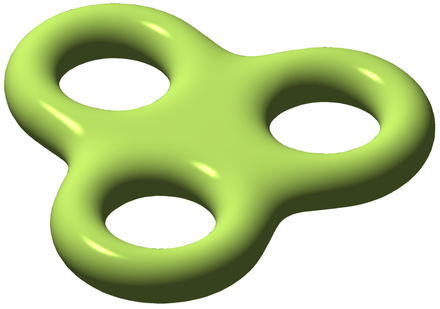
\includegraphics[scale = 1]{RiemannSurface}
**** Riemann Surface of genus 3, from Wikimedia ****

Of course this definition does not apply to curves over fields other than $\CC$, and doesn't relate the genus to the algebra of the curve. However, we can relate the topological genus of a curve directly to its topological Euler characteristic. Since $C$ is topologically compact, connected, and oriented, we have
$H^{0}(C; \ZZ)=H^{2}(C; \ZZ) = \ZZ$, so:
$
\chi_{top}(C) = 2-2g.
$
By the Hopf index theorem, the topological Euler characteristic is the degree of the tangent sheaf, or equivalently, minus the degree of the cotangent sheaf $\omega_{C}$; that is, $\deg K_{C} = 2g-2$, and thus
$$
g(C) = \frac{\deg(K_C)}{2} + 1.
$$
This formula serves to define the genus of a smooth projective curve over any field. 
Other characterizations of the genus require more machinery to establish. We will state some here, and use  tools from the following section to prove equivalence.

\begin{enumerate}

\item 
$
g(C) = 1 - \chi(\cO_C). \label{pa}
$

\item\label{genus Hilbert} If $C \subset \PP^r$ is a smooth curve of degree $d$  with homogeneous coordinate ring
$S_C$, then for sufficiently large $d$ the function $m \mapsto h_C(m) := \dim_\CC (S_C)_m$ is equal to a linear function
$$
p_C(m) =  dm - g + 1,
$$
so $g(C) = dm+1-p_C(m)$. 

\item\label{genus 1forms} $g(C)$ is the dimension of the vector space of regular 1-forms (that is, global sections of the
canonical sheaf) on $C$.
\end{enumerate}

\subsection{Arithmetic genus and geometric genus}
In this section, we'll deal with a  curve $C_0$ that is assumed to be reduced and irreducible.
Any reduced, irreducible 1-dimensional scheme $C_0$ has a normalization $\nu: C \to C_0$ which is a birational
map from a smooth curve. The genus of $C$ is called the \emph{geometric genus} of $C_0$.


The geometry of singular curves is a fascinating topic, from the local analysis of the singularities to the global questions involving linear series on singular curves, and most of the results of this book have analogues for singular curves. But this is a topic beyond the scope of this book; for us, the questions are about smooth curves, with singular curves appearing as a useful adjunct, for example in Chapter~\ref{PlaneCurveChapter}.

Applied to a possibly singular or even non-reduced 1-dimensional projective scheme, the formula~\ref{pa} and the equivalent~\ref{genus Hilbert}, define
what is called the \emph{arithmetic genus} $p_a(C)$. 

We can relate the two notions via the map of sheaves
$$
\cO_{C} \to \nu_*\cO_C.
$$
This is injective; the cokernel sheaf will be a skyscraper sheaf supported exactly on the singular points of $C_0$. Denoting this sheaf by $\cF$, we have an exact sequence
$$
0 \to \cO_{C_0} \to \nu_*\cO_C \to \cF \to 0.
$$

The normalization map $\nu: C \to C_0$ is finite, so that the higher direct images $R^i\nu_*\cO_C = 0$ for $i > 0$; it follows from the Leray spectral sequence that $\chi(\nu_*\cO_C) = \chi(\cO_C)$. Thus
$$
p_a(C_0) - g(C) =  \chi(\cO_{C}) -   \chi(\cO_{C_0}) = \chi(\cF) = h^0(\cF);
$$ 
in other words, the difference between the arithmetic and geometric genera of $C_0$ is the sum of the vector space dimensions of the stalks on $\cF$; colloquially, it's the number of linear conditions a function $f$ on $C$ has to satisfy to be the pullback of a function from $C_0$. The length of the stalk of $\cF$ at a particular singular point $p \in C_0$ is called the \emph{$\delta$-invariant of the singularity}; to rephrase the statement above in these terms, we have
$$
p_a(C_0) - g(C) = \sum_{p \in (C_0)_{sing}} \delta_p
$$ 

The $\delta$ invariant of a singularity is easy to compute in simple cases. For example:
\begin{enumerate}

\item (nodes) If $p \in C_0$ is a node, with points $r,s \in C$ lying over it, the condition for a function $f$ on $C$ to descend is simply that $f(r)=f(s)$; this is one linear condition and accordingly $\delta_p = 1$.

\item (cusps) If $p \in C_0$ is a cusp, with  $r \in C$ lying over it, the condition for a function $f$ on $C$ to descend is simply that the derivative $f'(r)=0$; again, this is one linear condition and accordingly $\delta_p = 1$.

\item (tacnodes) Suppose now that $p \in C_0$ is a \emph{tacnode}, that is, $C_0$ has two smooth branches at $p$ simply tangent to one another. There will be two points $r, s \in C$ lying over it, and the condition for a function $f$ on $C$ to descend is that in terms of suitable local coordinates both $f(r)=f(s)$ and $f'(r)=f'(s)$.  This represents two linear conditions and accordingly $\delta_p = 2$.

\item (planar triple points) Next up, consider an ordinary triple point $p \in C_0$ of a plane curve: that is, a singularity consisting of three smooth branches meeting pairwise transversely, such as the zero locus of $y^3-x^3$. There will be three points $r,s,t \in C$ lying over $p$, and certainly a necessary condition for a function $f$ on $C$ to descend is that $f(r)=f(s)=f(t)$---two linear conditions. But there's a third, less obvious linear condition: in order for $f$ to descend, the derivatives $f'(r), f'(s), f'(t)$ have to satisfy a linear condition---a reflection of the fact that a function on $C_0$ cannot vanish to order 2 on each of two branches without vanishing to order 2 along the third as well. Thus $\delta_p = 3$

\item (spatial triple points) We will be concerned in what follows only with planar singularities, but spatial triple points provide a useful contrast to the last example. A spatial triple point is a singularity consisting of three smooth branches, with linearly independent tangent lines, so that its Zariski tangent space is 3-dimensional. An example would be the union of the three coordinate axes in $\AA^3$.

In this case, in contrast to the last one, the condition that $f(r)=f(s)=f(t)$ is both necessary and sufficient for $f$ to descend, and accordingly we have $\delta_p=2$.

\end{enumerate}

\begin{exercise}
Let $p \in C$ be a singular point of a reduced curve $C$. Show that if $\delta_p = 1$, then $p$ must be either a node or a cusp.
\end{exercise}



\subsection{The Riemann-Roch Theorem}

To prove that these formulas for the genus are correct, we use \trr and Serre duality (sometimes called Kodaira-Serre duality, since Kodaira was responsible for the analytic version.)

\begin{theorem}[Riemann-Roch Theorem]\label{RR}
 If $C$ is a smooth, connected projective curve of genus $g$, and $D$ a divisor of degree $d$ on $C$ then
$$
h^0(D) = d - g + 1 + h^0(K_C - D).
$$
\end{theorem}

For example, if we take $D=0$, this tells us that $h^0(K) = g$, proving the characterization~(\ref{genus 1forms}) above. Using this and \trr for $D=K$
we get $\deg K = 2g-2$. Also, since $h^0(D) = 0$ for any divisor $D$ of negative degree, the formula gives the dimension of $h^{0}(D)$ when $\deg D$ is large:

\begin{corollary}\label{nonspecial RR}
For any divisor $D$ of degree $d$ we have
$$
h^0(D) \geq d - g + 1,
$$
with equality if $d > 2g-2$.
\end{corollary}
This was the theorem originally proven by Riemann; his student Roch supplied the correction term $h^0(K_C - D)$ for divisors of lower degree.
The dimension $h^0(K_C-D) = h^1(D)$ was called the \emph{superabundance} of $D$.

Corollary~\ref{nonspecial RR} and Proposition~\ref{very ample} together show that all high degree divisors come from hyperplane sections in 
suitable embeddings:

\begin{corollary}\label{degree 2g+1 embedding}
Let $D$ be a divisor of degree $d$ on a smooth, connected projective curve of genus $g$. If $d \geq 2g$, the complete linear series $|D|$ is base point free; and if $d \geq 2g+1$ the associated morphism $\phi_D : C \to \PP^{d-g}$ is an embedding, so that
$D$ is the preimage of the intersection of $C$ with a hyperplane in $ \PP^{d-g}$.
\end{corollary}

Since the complement of a hyperplane in projective space is an affine space, we get an affine embedding result too:

\begin{corollary}
 If $C$ is any smooth, connected projective curve and $\emptyset \neq \Gamma \subset C$ a finite subset then $C \setminus \Gamma$ is affine.
\end{corollary}
\begin{proof}
Let $D$ be the divisor defined by $\Gamma$. By Corollary~\ref{degree 2g+1 embedding} a high multiple of $D$ is very ample,
and gives an embedding $\phi: C\to \PP^n$ such that the preimage of the intersection of $C$ with some hyperplane $H$
is a multiple of $D$. It follows that $C\setminus \Gamma$ is embedded in $\AA^n = \PP^n\setminus H$.
\end{proof}
 
We can  use Corollary~\ref{nonspecial RR} to determine the Hilbert polynomial of a projective curve. To do this, let $C \subset \PP^r$ be a smooth curve of degree $d$ and genus $g$, and consider the exact sequence of sheaves
$$
0 \rTo \cI_{C/\PP^r}(m) \rTo \cO_{\PP^r}(m) \rTo \cO_C(m) \rTo 0
$$
and the corresponding exact sequence
$$
 H^0(\cO_{\PP^r}(m)) \rTo^{\rho_m} H^0(\cO_C(m)) \rTo H^1(\cI_{C/\PP^r}(m)) \rTo 0.
$$

The \emph{Hilbert function} $h_C$ of $C$  is defined by
$$
h_C(m) = \dim_{\CC} (S_{C})_{m} = \rank(\rho_m).
$$
By Theorem~\ref{Serre vanishing} we have $H^1(\cI_{C/\PP^r}(m)) = 0$ for large $m$, so $h_{C}(m) = h^0(\cO_C(m))$ for large $m$, which, by the Riemann-Roch theorem, equals $md-g+1$, again for large $m$. Thus, the Hilbert polynomial of $C \subset \PP^r$ is $p_C(m) = dm-g+1$, establishing the characterization~(\ref{genus Hilbert}).
 
The Riemann-Roch formula does \emph{not} give us a formula for the dimension $h^0(D)$ when $h^0(K_C - D)>0$; such divisors $D$ are called \emph{special divisors}, or \emph{special divisor classes}. The existence or non-existence of divisors $D$ with given $h^{0}(D)$ and $h^{1}(D)$ often serves to distinguish one curve from another, and will be an important part of our study.

\begin{fact}
If $k$ is a field that is not algebraically closed there may be smooth projective genus 0 curves over $k$ that are not isomorphic to $\PP^1$. However, they must be ``forms'' of $\PP^1$ in the sense that they become isomorphic to $\PP^1$ after extension of scalars to 
the algebraic closure $\overline k$ of $k$. The unique example with $k = \RR$ is the conic $x^2+y^2+z^2 = 0$. Indeed, any form of $\PP^1$ over any field $k$ can  be embedded in $\PP_{k}^2$  using the anti-canonical linear system.

The curve $\PP_k^1$ itself may be described as the scheme of left ideals of $k$-vector-space dimension 1 in the ring of
$2\times 2$ matrices over $k$ (such an ideal can be embedded in the matrix ring as a linear combination of the 2 columns in an appropriate sense). More generally, any scheme that is a form of $\PP^1$ over $k$
may be described as the scheme of 1-dimensional left ideals in a 4-dimensional central simple ($=$ Azumaya) algebra over $k$. For example, the
conic $x^2+y^2+z^2 = 0$ with no points over $\RR$ is the scheme of left ideals in the algebra of quaternions.\end{fact}

\subsection{A partial proof}

If, following~\ref[Chapter IV]{H} we take the definition of the genus of  a smooth connected curve $C$ to be $h^1(\sO_C)$ (so that $g = h^0(K_C)$ becomes a Corollary of Theorem~\ref{sd}), then it is easy to establish the following form of the Riemann-Roch Theorem:

\begin{corollary}
 If $C$ is a smooth, connected projective curve and $D$ is a divisor on $C$ then
$$
\chi(\sO_C(C)) := h^0(D) - h^1(D) = d-g+1
$$
or in other words, for any invertible sheaf $\cL$ of degree $d$ on $C$,
$$
\chi(\cL) = d-g+1.
$$
\end{corollary}
\begin{proof}
 Taking $D=0$ the statement becomes $h^0(\sO) - h^1(\sO) = 1-g$, which is our definition of $g$. On the other hand,
for any divisor $D$ on $C$ and any point $p \in C$ we have an exact sequence of sheaves
$$
0 \to \cO_C(D-p) \to \cO_C(D) \to \frac{\cO_C(D)}{\gm_{C,p}\cO_C(D)} \to 0
$$
Since $\cO_C(D)$ is locally isomorphic to $\sO_C$ we see that $\cO_C(D)/\gm_{C,p}\cO_C(D)\cong \kappa(p)$ is a sky-scraper sheaf of dimension 1, concentrated at $p$,
and thus has Euler characteristic 1. 
\end{proof}


Thus the Riemann-Roch Theorem for $\cO_C(D)$ is equivalent to the Riemann-Roch Theorem for $\cO_C(D-p)$. Since any divisor can be obtained from 0 by adding and subtracting points, the Riemann-Roch formula for an arbitrary $\cL$ follows from the special case $\cL = \cO_C$.

\subsection{Clifford's theorem}

While the Riemann-Roch Theorem gives a lower bound for the dimension of a linear system, $r(\sL) := h^0(\sL)-1 \geq \deg \sL -g$, Clifford's Theorem
gives an upper bound. If $\deg \sL>2g-2$, then the Riemann-Roch inequality becomes an equality, so it is enough to treat the case $\deg \sL \leq 2g-2$.
To state the sharpest form, we define a curve $C$ of genus $\geq 2$ to be \emph{hyperelliptic} if there exists a $g^1_2$ on $C$; that is an
invertible sheaf $\cL$ of degree $2$ with 2 independent global sections. We will see in Chapter~\ref{genus 2 and 3 chapter} that such a sheaf would be unique, and $h^0(\cL) = 2$.


\begin{theorem}\label{Clifford}
Let $C$ be a curve of genus $g$ and $\cL$ a line bundle of degree $d \leq 2g-2$. Then
$$
r(\cL) \leq \frac{d}{2}.
$$
Moreover, if  equality holds then we must have either
\begin{enumerate}
\item $d=0$ and $\cL = \cO_C$;
\item $d = 2g-2$ and $\cL = K_C$; or
\item $C$ is hyperelliptic, and $|\cL|$ is a multiple of the $g^1_2$ on $C$.
\end{enumerate}
\end{theorem}

\fix{We haven't defined ``hyperelliptic" at this point, or talked about ``the $g^1_2$". Should we just state the weak form of Clifford here, or should we move the definition of hyperelliptic?}

The proof of the inequality will follow easily from a basic result about the addition of linear series, defined as follows:
$\cD = (\cL,V)$ and $\cE = (\cM, W)$ be two linear series on a curve $C$. By the \emph{sum} $\cD + \cE$ of $\cD$ and $\cE$, we will mean the pair 
$$
\cD + \cE = (\cL \otimes \cM, U) 
$$
where $U \subset H^0(\cL \otimes \cM)$ is the subspace generated by the image of $V \otimes W$, under the multiplication/cup product map $H^0(\cL) \otimes H^0(\cM) \to H^0(\cL \otimes \cM)$---in other words, it's the subspace of the complete linear series $|\cL\otimes \cM|$ spanned by divisors of the form $D+E$, with $D \in \cD$ and $E \in \cE$.
 
\begin{proof}
If $\cD$ and $\cE$ are two nonempty linear series on a curve $C$, then
$$
\dim(\cD + \cE) \geq \dim \cD + \dim \cE.
$$
To see this, we observe that to say $\dim \cD \geq m$ means exactly that we can find a divisor $D \in \cD$ containing any given $m$ points of $C$; since $\cD + \cE$ contains all pairwise sums $D + E$ with $D \in \cD$ and $E \in \cE$, we can certainly find a divisor $F \in \cD + \cE$ containing any given $\dim \cD + \dim \cE$ points of $C$.

The proof of the inequality in Clifford's Theorem follows  by applying this observation to the pair $|\cL|$ and $|K_C\otimes \cL^{-1}|$: by 
the Riemann-Roch Theorem, we have
$$
r(K_C\otimes \cL^{-1}) = r(\cL) +g - d - 1
$$
and so we deduce that
$$
g = r(K_C) + 1 \geq r(\cL) + r(K_C\otimes \cL^{-1}) + 1 \geq 2r(\cL) +g - d;
$$
hence $r(\cL) \leq d/2$.

For the proof of the second half of Clifford we will use a basic fact about the geometry of hyperplane sections of a curve in projective space (Proposition~\ref{monodromy of hyperplane section}); we defer it to there.
\end{proof}



\section{The canonical morphism}

Given the central role played by the canonical divisor class, it is natural to look at the geometry of the morphism $\phi_K : C \to \PP^{g-1}$ associated to the complete canonical series $|K|$.  

\begin{definition}
A curve $C$ of genus $g \geq 2$ is said to be \emph{hyperelliptic} if there exists a morphism $f: C \to \PP^1$ of degree 2. \end{definition}

\begin{theorem}\label{canonical system is very ample}
If $C$ is a smooth curve of genus $\geq 2$ then the canonical morphism $\phi_K : C \to \PP^{g-1}$ is an embedding if and only if $C$ is not hyperelliptic.
\end{theorem}

\begin{proof}
By Corollary~\ref{degree 2g+1 embedding} we have to show that for any pair of points $p, q \in C$ we have
$$
h^0(K_C(-p-q)) = h^0(K_C)-2 = g-2.
$$
Applying \trr we see this fails if and only if $h^0(\cO_C(p+q)) \geq 2$ for some $p,q \in C$. By Lemma~\ref{deg 2 morphism}, this implies that $C$ is hyperelliptic.
\end{proof}

\begin{lemma}\label{deg 2 morphism}
Let $C$ be a smooth, projective curve of genus $g\geq 2$. If $C$ has an invertible sheaf $\cL$ of degree 2 with two independent sections, then
$|\cL|$ defines a morphism of degree 2 to $\PP^{1}$, and $C$ is hyperelliptic. In particular, if $g(C) = 2$ then the canonical series $|K_{C}|$ defines a 2 to 1 morphism to $\PP^{1}$, so $C$ is hyperelliptic.
\end{lemma}

\begin{proof}
If $\cO_C(p+q)$ has two independent sections and has $d$ basepoints, then it defines a morphism of degree $2-d$ to $\PP^1$. Since $C$ is not rational,
we must have $d=0$, proving the first statement. 
\end{proof}

\subsection{The geometric Riemann-Roch theorem}

If $C$ is a nonhyperelliptic curve, embedded in $\PP^{g-1}$ by its canonical series and  $D = p_1+\dots + p_d$ is a divisor consisting of $d$ distinct points, let $\overline D$ be the span of the points $p_i \in C \subset \PP^{g-1}$. Since the hyperplanes in $\PP^{g-1}$ containing $\{p_1,\dots,p_d\}$ correspond (up to scalars) to sections of $K_C$ vanishing at all the points $p_i$, we see that
$$
h^0(K_C-D) = g - 1 - \dim \overline D.
$$
Plugging this into the Riemann-Roch formula, we arrive at the statement
$$
r(D) = d - 1 - \dim \overline D;
$$
or in other words, the dimension of the linear series $|D|$ in which the divisor $D$ moves is equal to the number of linear relations on the points $p_i$ on the canonical curve. Thus, for example, if $D = p_1+p_2+p_3$, we see that $D$ moves in a pencil if and only if the points $p_i$ are collinear.

We can extend this statement to the case of arbitrary effective divisors $D$ on any smooth curve if we define our terms correctly. To do this, suppose $f : C \to \PP^d$ is any morphism, and $D \subset C$ any divisor. We define the \emph{span} of  $f(D)$ to be the intersection
$$
\overline{f(D)} = \bigcap_{H \mid f^{-1}(H)\supset D} H 
$$
of all hyperplanes in $\PP^d$ whose preimage in $C$ contains $D$. The argument above applies to prove:

\begin{theorem}[Geometric Riemann-Roch Theorem]\label{geometric RR}
If $C$ is any curve of genus $g \geq 2$,  $\phi : C \to \PP^{g-1}$ its canonical morphism and $D \subset C$ any effective divisor of degree $d$, then
$$
r(D) = d - 1 - \dim \overline{\phi(D)}.
$$
\end{theorem}
 
 \section{Canonical Curves}\label{Noether theorem section}

When we analyze the embedding of a curve $C\subset \PP^n$ we generally ask first whether $C$ is contained in any low-degree
hypersurfaces, and if so how many, in the sense of the dimension $(I_C)_d)$ the degree $d$ part of the homogeneous ideal of $C$.
From the long exact sequence in cohomology
$$
0\to H^0(\sI_{C/\PP^n}(d)) \to H^0(\sO_{\PP^n}(d)) \to H^0(\sO_C(d)) \to H^1(\sI_{C/\PP^n}(d)) \to H^1(\sO_{\PP^n}(d)) \to\cdots
$$
together with the facts that  $H^0(\sO_{\PP^n}(d))$ is the vector space of degree $d$ forms on $\PP^n$ and 
 $H^1(\sO_{\PP^n}(d)) = 0$ for $n>1$ and $d\geq 0$, we see that
 $$
 \dim (I_C)_d = h^0(\sI_{C/\PP^n}(d)) = h^0(\sO_{\PP^n}(d)) - h^0(\sO_C(d)) + h^1(\sI_{C/\PP^n}(d)).
$$
If $d$ times the degree of $C$ is $>2g-2$, the the Riemann-Roch Theorem tell us the value of
 $h^0(\sO_C(d))$, and thus a lower bound for $ \dim (I_C)_d$, but if, in addition, the map
 $H^0(\sO_{\PP^n}(d) \to H^0(\sO_C(d))$ is surjective (or equivalently $h^1(\sI_{C/\PP^n}(d))=0$),
 then we get $ \dim (I_C)_d$ exactly.
 
 
\begin{definition} An embedding of a smooth curve
$C\subset \PP^n$ is said to be \emph{projectively normal} if all the maps $H^0(\sO_{\PP^n}(d)) \to H^0(\sO_C(d))$ are surjective,
or equivalently $h^1(\sI_{C/\PP^n}(d))=0$ for all $d\geq 0$.
\end{definition}
 
By Serre's Criterion of Normality  a 1-dimensional scheme  $C\subset \PP^n$
is a smooth, projectively normal curve iff the homogeneous coordinate ring of $C$ is a normal ring, whence the terminology in
this definition. The criterion has two parts, which are interesting separately: A local or graded ring is normal if it is nonsingular in
codimension 1; and
locally of depth $\geq 2$ in codimension $\geq 2$. In the case of the homogeneous coordinate ring of a curve, 
the first condition means that the curve is nonsingular and the second means that $h^1(\sI_{C/\PP^n}(d))=0$ for all $d$.
In particular, for any very ample invertible sheaf $\sL$ on a smooth curve $C$, the ring 
$$
R(C, \sL) := \bigoplus_{m=0}^\infty H^0(\sL^m)
$$
is normal. See for example \cite[Theorem ***]{Eisenbud1995}.

\begin{example}\label{rnc is projectively normal}
For $d\geq 1$ the rational normal curve $C\subset \PP^d$ of degree $d$ is projectively normal. 
We have $H^0(\sO_{\PP^1}(md))  = \CC[s,t]_{md}$. Th natural natural map
$$
\CC[x_0,\dots,x_d] \to\bigoplus_{m = 0}^\infty H^0(\sO_{\PP^1}(md)));\quad x_0,\dots, x_d \mapsto s^d,s^{d-1}t,\dots, t^d
$$ 
is surjective since every monomial of degree $md$ can be written as a monomial in  
the elements $s^d,s^{d-1}t,\dots, t^d$, and the ring is normal (Exercise~\ref{normality of RNC}).
\end{example}

\begin{exercise}\label{normality of RNC}
 Show that $\CC[s^d,s^{d-1}t,\dots, t^d]$ is normal (ie, integrally closed) by noting that its integral closure must be
 contained in $\CC[s,t]$ and then showing that if $f$ is any polynomial
 in the integral closure then the homogeneous components of $f$ are also in the integral closure.
\end{exercise}


We will now show that the canonical image of a smooth curve is always projectively normal. When the curve is hyperelliptic,
the canonical image is the rational normal curve, treated above, so we may assume that the curve $C$ is embedded
by $|K_C|$ as a smooth curve in $\PP^{g-1}$.


To do this we will make use of an auxiliary construction, a \emph{simple $(g-4)$-secant $(g-3)$-plane.}

\begin{lemma}
 If $C\subset \PP^n$ is a reduced, irreducible, nondegenerate curve, and $m\leq n-1$, then the linear span $L := \overline{p_1,\dots, p_m}$
 of $m$ general points of $C$ is a simple $m$-secant; that is, a plane of dimension $m-1$ such that
 $C\cap L = \{p_1,\dots,p_m\}$ scheme-theoretically.
 \end{lemma}
 
 
\begin{proof}
The plane $L$ is contained in a hyperplane $H$, and since the points are general, we may take this to be a general hyperplane. By Bertini's Theorem, $C\cap H$ is reduced, so $C\cap L$ is also reduced.
 If $C\cap L$ had length $>m$, then by Lemma~\ref{general position lemma} every set of $m+1$ points of $C\cap H$ would be dependent,
 and the span of $C\cap H$ would thus have dimension $\leq m-1<n-1$, and we could choose a hyperplane section $C\cap H'$ with more points than $C\cap H$, which is absurd.
\end{proof}

The following was proven by Max Noether, Emmy's father:

\begin{theorem}[Max Noether]\label{canonical curves are ACM}
A canonical curve in $\PP^{g-1}$ has degree $2g-2$ and arithmetic genus $g$. If the curve has a simple
$g-2$ secant, then it is arithmetically Cohen-Macaulay; that is,
$\HH^{1}(\sI_{C/\PP^{g-1}}(m)) = 0$ for all $m\in \ZZ$.
\end{theorem}
 
For a canonically embedded irreducible curve the simple $g-3$-dimensional $g-2$ secant planes $\Lambda$  correspond to base-point-free pencils of degree $g = 2g-2 -(g-2)$: Given $\Lambda$, the linear series of hyperplanes containing $\Lambda$ intersects $C$ in $\Lambda$ plus the fibers of this pencil. Conversely, given such a pencil, the plane is the span of the complement of a general  member $P$ of the pencil in  $C\cap \overline P$, where $\overline P$ is the hyperplane that is the linear span of $P$.
   
\begin{proof} The Hilbert polynomial $\chi_{C}(t) = h^{0}\sO(t)-h^{1}\sO(t)$ of $C$ has degree equal to
$\dim C = 1$, so it is determined by two values.

We begin by showing that $\sO(-m)$ has no global sections for $m>0$.
If $D$ is a divisor equivalent to $m$ times the hyperplane section, we have an exact sequence
$$
0\to \HH^{0}(\sO_{C}(-m)) \to \HH^{0}(\sO_{C}) \to \HH^{0}(\sO_{D}) \to \cdots.
$$
By hypothesis, the vector space $\HH^{0}\sO_{C}$ is spanned by the constant functions, and these
restrict non-trivially to $\sO_{D}$, and $\HH^{0}(\sO_{C}(-m)) = 0$ as claimed.

Using the Riemann-Roch Theorem we can now compute the Hilbert function $\chi_{C}(m)$:
We have 
\begin{align*}
 \chi_{C}(0) &= h^{0}(\sO_{C}) - h^{1}(\sO_{C}) = h^{0}(\sO_{C}) - h^{0}(\omega_{C}) = 1-g.\\
\chi_{C}(1) &= h^{0}(\sO_{C}(1)) - h^{1}(\sO_{C}(1)^{*}\otimes \omega_{C}) = h^{0}(\omega_{C}) - h^{0}(\sO_{C}) = g-1.
\end{align*}
and we deduce
$\chi_{C}(m) = (2g-2)m -g+1$, whence we see that the degree of $C$ is $2g-2$ and $p(C) = g$ as claimed.

To show that
$C$ is arithmetically Cohen-Macaulay we use the sequence
$$
\cdots \to \HH^{0}(\sO_{\PP^{n}}(m)) \to \HH^{0}(\sO_{C}(m))
\to \HH^{1}(\sI_{C}(m))\to \HH^{1}(\sO_{\PP^{n}}(m)) \to\cdots .
$$
Since $\HH^{1}(\sO_{\PP^{n}}(m)) = 0$, it
is enough to show that the natural map 
$$
\HH^{0}(\sO_{\PP^{n}}(m)) \to \HH^{0}(\sO_{C}(m))
$$
 is surjective for all $m\in \ZZ$. For $m=0,1$ this is immediate from the hypothesis.

For $m <0$ we must show $\HH^{0}(\sO_{C}(m))=0.$ 
If $D$ is a divisor equivalent to $-m$ times the hyperplane section, we have an exact sequence
$$
0\to \HH^{0}(\sO_{C}(m)) 
\to \HH^{0}(\sO_{C}) 
\to \HH^{0}(\sO_{D}) \to \cdots.
$$
By hypothesis, the vector space $\HH^{0}\sO_{C}$ is spanned by the constant functions, and these
restrict non-trivially to $\sO_{D}$, so the kernel, $\HH^{0}(\sO_{C}(m))$, is 0 as claimed. 

To prove surjectivity for $m\geq 2$ we use the remaining hypothesis, the existence of
a simple $g-3$-dimensional $g-2$ secant plane $\Lambda$  and an idea sometimes called the \emph{base-point-free pencil trick}. Let $p_{0},\dots p_{g-3}$ be the points in which $\Lambda$ meets $C$.  Since the
$p_{i}$ are linearly independent by hypothesis, we may choose homogeneous coordinates $x_{i} \in \HH^{0}(\sO_{C}(1))$ so that
$x_{i}(p_{j}) \neq 0$ if and only if $i = j$. It follows that the sections
$x_{i}^{m}$ of $\sO_{C}(m)$ span $\HH^{0}(\sO_{C}(m)|_{\{p_{0}, \dots, p_{g-3}\}})$. Let 
$V\subset \HH^{0}(\sO_{C}(1))$ be the two-dimensional subspace of linear forms vanishing on
$\Lambda$, and thus on the $p_{i}$. 

For $m\geq 2$ there are maps of vector spaces
$$
\wedge^{2} V\otimes \HH^{0}(\sO_{C}(m-2)) \to V\otimes \HH^{0}(\sO_{C}(m-1)) 
\to \HH^{0}(\sO_{C}(m))
$$
where the right hand map is multiplication and the left hand map sends
$s_{1}\wedge s_{2}\otimes \sigma$ to $s_{1}\sigma-s_{2}\sigma$ for any local section $\sigma$.
The sequence is exact because the sections $s_{1},s_{2}$ that span $V$ never vanish simultaneously except on the $p_{i}$, and has image  consisting of sections that vanish on the points $p_{i}$

\end{proof}

\begin{corollary}\label{canonical hilbert function}
If $C\subset \PP^{g-1}$ is a canonical curve with a simple $g-3$-secant, then the Hilbert function of the homogeneous coordinate ring $S_{C}$ of  $C$ depends only on $g$, and is given by:
$$
\dim({S_{C}})_{d} = h^{0}(\cO_{C}(d)) = 
\begin{cases}
 0 &\mbox {if } d<0\\
 1 & \mbox {if }  d=0\\
 g & \mbox {if }  d=1\\
 (2n-1)g+1 & \mbox {if }  d>1\\
\end{cases}
$$
\end{corollary}
\begin{proof}
Theorem~\ref{canonical curves are ACM} implies, in particular, that the homogeneous coordinate ring of $C$ can be identified with 
$\oplus_{n\in \ZZ}\HH^0\sO_C(n)$.  
\end{proof}

 \section{A bit about surfaces}
 We will often analyze curves  on a smooth surface; here are a few results that will be useful. We refer to~\cite[Chapter V]{Hartshorne1977}
 and~\cite[Chapter I]{Beauville} for proofs.
 
 We suppose for this section that $X$ is a smooth projective surface.
 We define $\Pic(X)$ to be the group whose elements are invertible sheaves on $X$.
When two divisors $D,E$ on $X$ meet transversely we define $D\cdot E$ to be the number of points in which they meet. If they have no common
components, we can still define a non-negative intersection multiplicity $m_X(D,E,p)$ at each point $p$, and then set
$$
D\cdot E = \sum_p m_X(D,E,p).
$$
Over the complex numbers each codimension 1 subvariety $D$ of $X$ has a fundamental class
$[D]\in H^2(X, \ZZ)$ and the product is the cup product with values in $H^4(X,\ZZ)$, which is $\ZZ$ since $X$ is compact and orientable. Thus
there is an extension of the product to the cases where $D,E$ have common components. From a geometric point of view, we may choose an
appropriate $C^\infty$
normal vector field along $E$ and define $E'$ by ``pushing'' $E$ out slightly along the direction of this field, until $D$ and $E'$ are transverse,
and the intersections can be computed in the usual way. It should be noted that such intersection numbers can be either positive or negative,
since they depend on the relative orientations of $D$ and $E'$ at the intersection points; this is in contrast to the case when $D$ and $E$
themselves meet properly; in this case the fact that the complex numbers are canonically oriented makes the intersection number non-negative.

The intersection product can also be defined algebraically, over any field: Setting $\sL := \sO_X(C)$ and
$\sM := \sO_X(D)$ to simplify the notation, we set 
$$
D\cdot E = \chi(\sO_X)-\chi(\sL^{-1}) -\chi(\sM^{-1}) -\chi(\sL^{-1}\sM^{-1}) 
$$
\begin{theorem} The pairing $(D,E) \mapsto (D.E)$ is the unique bilinear map
$\Pic(X) \times \Pic(X) \to \ZZ$ extending the case of intersections of two transverse curves on $X$. 
\end{theorem}

A frequent use of the the intersection pairing is to compute the (arithmetic) genus of a curve on a surface,
a result called the adjunction formula.

\begin{theorem}[Adjunction Formula]\label{adjuction formula}
If $C$ is a curve lying on a smooth surface $X$ then 
$$
\omega_C = \omega_X \otimes \sO_X(C) \otimes \sO_C.
$$
In particular \label{genus formula}
$$
p_a(C) = \frac{(K_X+C)\cdot C}{2} +1
 $$
\end{theorem}

We will frequently be interested in curves on quadrics in $\PP^3$, and we can spell out the
intersection theory on these surfaces very concretely; see for example~\cite[****]{Hartshorne1977}.
We will treat them and the curves on them in detail in Section~\ref{curves on scrolls} as part of the larger family of 2-dimensional rational normal scrolls; for
now we sketch the situation as an example of the theory of this section. 

\begin{example}[Quadrics in $\PP^3$]\label{Div of quadric}
 
Quadric surfaces $S$ in $\PP^3$ are classified by their rank:
\begin{itemize}
\item A quadric of rank 2 is the union of two planes; it cannot contain an nondegenerate irreducible curve
\item A rank 3 quadric $S$ is a cone over a plane conic. Suppose that $C$ is a smooth,
curve on such a quadric:
\begin{itemize}
\item  If $C$  does
not pass through the vertex then it is the intersection of the quadric with a hypersurface of some
degree $d$. In this case $C$ has degree $2d$ and genus $(d-1)^2$. 
 \item if $C$ passes through the vertex, then $C$ lies in the divisor class of a line through the origin plus the intersection of $S$ with a hypersurface of some degree $d$. In this case $C$ has degree $2d+1$ and 
 genus $d(d-1)$. 
\end{itemize}

%If  it contains smooth irreducible curves that do not pass through the vertex of the cone, and smooth irreducible curves that of
%degree $2d$ that are intersections of $S$ with hypersurfaces of degree $d$; and smooth 
%irreducible curves of degree $2d+1$ that 

\item A quadric of rank 4 is nonsingular, and is isomorphic to $\PP^1\times \PP^1$.


\item The Picard group of $\PP^1\times \PP^1$ is $\ZZ\oplus \ZZ$, generated by the 
classes of the lines $\{p\}\times \PP^1$ and $\PP^1\times \{p\}$, where $p\in \PP^1$
is any point. These lines have self-intersection 0, and meet transversely in a point,
so the intersection pairing is given by $(a,b)\cdot(c,d) = ad+bc$. From the adjunction formula
applied to the classes of the lines $(1,0)$ and $(0,1)$ we that the canonical
class is $(-2,-2)$, and thus the arithmetic genus of a curve of type $(a,b)$ is thus
$$
\left(((a,b)+(-2,-2))\cdot (a,b)\right)/2 +1 = (a-1)(b-1).
$$

\item Writing $\pi_1, \pi_2$ for the two projections of
$\PP^1\times \PP^1 \to \PP^1$, the sheaf 
$$
\sL := \sO_{\PP^1\times \PP^1}(a,b) = \pi_1^*\op1a \otimes \pi_2^*\op1b
$$
has cohomology given by the K\"unneth formula, for example
\begin{align*}
 H^0(\sL) &= H^0(\op1a)\otimes H^0(\op1b) \hbox{ and thus }\\
 h^0(\sL) &= (a+1)(b+1) \hbox{ if } a\geq 0, b\geq 0.
\end{align*}

\item Any smooth quadric surface $S\subset \PP^3$ is the 
image of $\PP^1\times \PP^1$ embedded by the complete linear system
$|\sO_{\PP^1\times \PP^1}(1,1)|$ and thus contains two families of lines. 
A curve in the class $(a,b)$ thus has degree $(a,b)\cdot(1,1) = a+b$. 
\end{itemize}
\end{example}

Often we wish to compute the dimension of the space of sections of an invertible sheaf, but
as with the case of curves, the Euler characteristic is more accessible:

\begin{theorem}[Riemann-Roch for surfaces] Let $\sL$ be an invertible sheaf on a smooth surface $S$.
the Euler characteristic $\chi(D) := h^0(\sL)-h^1(\sL)+h^2(\sL)$, where $\sL = \sO_S(D)$, is given by
$$
\chi(D) = \chi(\sO) + \frac{(D-K_S)\cdot D}{2}+1
$$
\end{theorem}

\fix{Possible addition:  the Hodge Index theorem as corollary. This could be used to prove finiteness of the automorphism group of a curve following Hartshorne V Ex. 1.11, perhaps in place of the proof now in the inflections chapter.}

It is useful to know what happens under mappings of surfaces, particularly the case of the mapping
corresponding to blowing up a point.

\begin{theorem}
If $\pi: X \to Y$ is a birational map of smooth surfaces, then the pullback map on divisors
preserves the intersection pairing. If $X$ is the blowup of $Y$ at a point $p$, with exceptional
divisor $E = \pi^{-1}(p)$ then:

\begin{enumerate}
 \item $\Pic X =\pi^*(\Pic Y) \oplus \ZZ E$.
\item The canonical class on $X$ is given by $K_X = \pi^*(K_Y)+E$.
 \item The intersection pairing on $\Pic X$ is given by
 
\begin{itemize}
\item $\pi^*(D)\cdot\pi^*(D') = D.D'$ for all $D,D'\in \Pic Y$.
\item $\pi^*(D)\cdot E = 0$ for all $D\in \Pic Y$.
 \item $E\cdot E = -1$.
 \item $K_X\cdot E = -1$.
 \item If $C$ is a curve that has an $m$-fold point at $p$ then $\pi^{-1}(C)$ contains $E$ with multiplicity $m$.
 \end{itemize}
\end{enumerate}
\end{theorem}

Blowups occur frequently in the theory of surfaces, and are easy to characterize:
\begin{theorem}
If $E\subset X$ is a curve on a smooth projective surface $X$ and
 that $E^2 = E\cdot K_X = -1$ then $E$ can be ``blown down'' in the sense that
 $X$ is the blowup of a smooth surface $Y$ at a point $p\in Y$, and $E$ is the exceptional divisor.
\end{theorem}


\input footer.tex
%header and footer for separate chapter files

\ifx\whole\undefined
\documentclass[12pt, leqno]{book}
\usepackage{graphicx}
\input style-for-curves.sty
\usepackage{hyperref}
\usepackage{showkeys} %This shows the labels.
%\usepackage{SLAG,msribib,local}
%\usepackage{amsmath,amscd,amsthm,amssymb,amsxtra,latexsym,epsfig,epic,graphics}
%\usepackage[matrix,arrow,curve]{xy}
%\usepackage{graphicx}
%\usepackage{diagrams}
%
%%\usepackage{amsrefs}
%%%%%%%%%%%%%%%%%%%%%%%%%%%%%%%%%%%%%%%%%%
%%\textwidth16cm
%%\textheight20cm
%%\topmargin-2cm
%\oddsidemargin.8cm
%\evensidemargin1cm
%
%%%%%%Definitions
%\input preamble.tex
%\input style-for-curves.sty
%\def\TU{{\bf U}}
%\def\AA{{\mathbb A}}
%\def\BB{{\mathbb B}}
%\def\CC{{\mathbb C}}
%\def\QQ{{\mathbb Q}}
%\def\RR{{\mathbb R}}
%\def\facet{{\bf facet}}
%\def\image{{\rm image}}
%\def\cE{{\cal E}}
%\def\cF{{\cal F}}
%\def\cG{{\cal G}}
%\def\cH{{\cal H}}
%\def\cHom{{{\cal H}om}}
%\def\h{{\rm h}}
% \def\bs{{Boij-S\"oderberg{} }}
%
%\makeatletter
%\def\Ddots{\mathinner{\mkern1mu\raise\p@
%\vbox{\kern7\p@\hbox{.}}\mkern2mu
%\raise4\p@\hbox{.}\mkern2mu\raise7\p@\hbox{.}\mkern1mu}}
%\makeatother

%%
%\pagestyle{myheadings}

%\input style-for-curves.tex
%\documentclass{cambridge7A}
%\usepackage{hatcher_revised} 
%\usepackage{3264}
   
\errorcontextlines=1000
%\usepackage{makeidx}
\let\see\relax
\usepackage{makeidx}
\makeindex
% \index{word} in the doc; \index{variety!algebraic} gives variety, algebraic
% PUT a % after each \index{***}

\overfullrule=5pt
\catcode`\@\active
\def@{\mskip1.5mu} %produce a small space in math with an @

\title{Personalities of Curves}
\author{\copyright David Eisenbud and Joe Harris}
%%\includeonly{%
%0-intro,01-ChowRingDogma,02-FirstExamples,03-Grassmannians,04-GeneralGrassmannians
%,05-VectorBundlesAndChernClasses,06-LinesOnHypersurfaces,07-SingularElementsOfLinearSeries,
%08-ParameterSpaces,
%bib
%}

\date{\today}
%%\date{}
%\title{Curves}
%%{\normalsize ***Preliminary Version***}} 
%\author{David Eisenbud and Joe Harris }
%
%\begin{document}

\begin{document}
\maketitle

\pagenumbering{roman}
\setcounter{page}{5}
%\begin{5}
%\end{5}
\pagenumbering{arabic}
\tableofcontents
\fi


\chapter{The Riemann--Roch theorem}\label{RiemannRochChapter}

\section{How many sections?}

To study curves via their maps to projective spaces, we want to estimate the dimension of the space of global
sections of an invertible sheaf $\cL$. The beginning
of the story is the Riemann--Roch theorem.

Though we would like to be able to compute $h^0(\sL)$, it is much
easier to compute the 
\blue{Euler characteristic}
\index{Euler characteristic}%
$$
\chi(\sL):= \sum_{i\geq 0} (-1)^i h^i(\sL).
$$
This computes $h^0(\cL)$ itself in many cases, by virtue of the following result:
\marginpar{indexed theorem name}

\begin{theorem}[Serre--Grothendieck vanishing theorem]
\label{Serre--Grothendieck vanishing}
\index{Serre--Grothendieck vanishing theorem}%
\index{vanishing theorem!Serre--Grothendieck}%
If $\sF$ is a coherent sheaf on a projective scheme $X$ of dimension $n$, then for any $i$, the vector space $H^i(\sF)$ is finite-dimensional, and is 0 if  $i> n$. Moreover,
if $X\subset \PP^m$ then for $d\gg 0$, $\sF(d)$ is generated by its global sections and $H^i(\sF(d)) = 0$ for all $i>0$.\qed
\end{theorem}

\begin{proof}
This is a combination of 
theorems due to Grothendieck and Serre. See
\cite[Theorems III.2.7 and III.5.2]{Hartshorne1977}, 
and
also \cite{Serre1955} for a 
reasonably
concrete proof.
\end{proof}

A 
shortcoming
of this vanishing theorem is the lack of a bound on the number $d$ needed to achieve the second assertion. For smooth curves
and invertible sheaves
this is corrected by Theorem~\ref{RR theorem}, which gives a bound in terms of the genus and the degree.

One immediate consequence of Theorem~\ref{Serre--Grothendieck vanishing} is that on a smooth variety the groups of invertible sheaves and divisor classes are the same:

\begin{corollary}\label{invertible sheaves and divisors}
If $X$ is a projective variety that is nonsingular in codimension $1$,
every invertible sheaf $\cL$ on $X$ is of the form $\cL =\cO_C(D)$ for some 
\index{Cartier divisor}\index{divisor!Cartier}%
Cartier divisor $D$ on $X$. Thus if $X$ is a smooth projective variety
\index{notation!div}%
the map $\div$ is an isomorphism from the group of invertible sheaves
to the group 
of divisor classes.
\end{corollary}

\begin{proof}
Let $H \subset \PP^r$ be a general hyperplane, and $E$  the divisor  of intersection of $C$ with $H$. We know that for $n \gg 0$, $\cL(n)$ has sections; and if $F$ is the divisor of zeroes of one such section, we have
$$
\cL = \cO_C(F - nE).
$$
If $X$ is smooth, then, since a regular local ring is a unique
factorization domain, every codimension-one subvariety is defined locally 
by a single nonzerodivisor, and thus corresponds to a Cartier divisor.
This implies that $\div$ is surjective. Furthermore any 
\blue{isomorphism between invertible sheaves}
\index{invertible sheaf!isomorphism between -s}%
is defined by multiplication with a global rational function, so that invertible sheaves defining linearly equivalent divisors are
isomorphic. Thus $\div$ is injective as well.
\marginpar{(de): this proof is pretty swift, and the result fundamental. Let's give a Hartshorne citation too.}
\end{proof}

\subsection*{Riemann--Roch without duality}

It follows from Theorem~\ref{Serre--Grothendieck vanishing} that on
any scheme $X\subset \PP^r$ we have $\chi(\sL(d)) = h^0(\sL(d))$ for
large $d$, 
and that $\chi(\sL) = h^0(\sL) - h^1(\sL)$ in the case of a curve.

\begin{theorem}[easy Riemann--Roch]\label{easy RR}
If $C$ is a smooth projective curve, and $\sL$ is an invertible sheaf on $C$, then $\chi(\sL) = \deg \sL + \chi(\sO_C)$.
\index{Riemann--Roch theorem!easy}%
\end{theorem}

\begin{proof}
 The result is tautological if $\sL = \sO_C$. Every invertible sheaf on $C$ has the form $\sL = \sO_C(D)$ for some
divisor $D$. If $p\in C$, then writing $\kappa(p)$ for the
structure sheaf of the subscheme $p\in C$, the long exact sequence in cohomology
associated to the short exact sequence
$$
0\to \sL(-p) \to \sL \to \sL\otimes \kappa(p)\to 0
$$
together with the isomorphism $\sL\otimes \kappa(p) \cong \kappa(p)$
and the vanishing of higher cohomology of a sheaf with zero-dimensional support allows us to compute 
$$
\chi(\sL) = \chi(\sL(-p)) + \chi(\kappa(p)) = \chi(\sL(-p)) + 1.
$$
Since every divisor on $C$ can be reached by adding and subtracting points, this suffices.
\end{proof}

Since the Euler characteristic of a sheaf is well-behaved, we can extend the result of Theorem~\ref{easy RR} 
to invertible sheaves on any one-dimensional scheme $C$, by defining
$\deg \sL := \chi(\sL) -\chi(\sO_C)$.
We will use this definition to express the self-intersection of a divisor on a surface in Section~\ref{surface basics}.

We can make the Riemann--Roch theorem still more useful by understanding the error term $h^1(\sL)$. This requires
the canonical divisor and Serre duality, to which
we now turn.


\section{The most interesting linear series}\label{most interesting}

The most important vector bundles on a manifold are the tangent and cotangent bundles. For reasons that
will become clear, the focus in algebraic geometry is on the cotangent
bundle or, equivalently, the sheaf of differential 1-forms. On a
smooth curve $C$ the \emph{canonical sheaf} is the sheaf of
differentials, which is an 
\index{canonical sheaf}\index{sheaf!canonical}\index{sheaf!of differentials}%
invertible sheaf; on a smooth
variety of dimension $n$ we define the canonical sheaf to be the 
$n$-th exterior power of the sheaf of differentials. A section of 
$\omega_C$ is thus a differential form, and the class of the divisor
of such a form is usually denoted 
\blue{$K_C$.}
\index{notation!$K_C$}%

\begin{fact}
Canonical sheaves are defined for any projective scheme; see 
Definition~\ref{dualizing sheaf for singular curve}.
They are usually called 
\index{dualizing sheaf}\index{sheaf!dualizing}%
{\it dualizing sheaves} 
in that generality. The condition for the dualizing sheaf to be an invertible
\index{Gorenstein scheme}%
sheaf is that the scheme is (locally) Gorenstein, something that is true, for example, for any subscheme of $\PP^r$
that is locally a complete intersection (see Section~\ref{dualizing sheaves section}).
\end{fact}
 

On projective space we can compute the canonical sheaf directly; other computations of the canonical sheaf will usually reduce to this central case.

\begin{theorem}
 The 
\blue{canonical sheaf of $\PP^{r}$}
\index{canonical sheaf!of $\PP^{r}$}%
is $\sO_{\PP^{r}}(-r-1)$. 
\vspace*{-\parskip}
\end{theorem}

\begin{proof}
Let $x_{0}, \dots, x_{r}$ be the projective coordinates on $\PP^{r}$
and let  $U = \PP^{r}\setminus H$ be the affine open set where $x_{0}
\neq 0$. Thus $U \cong \AA^{r}$ with coordinates $z_{1} :=
x_{1}/x_{0}$, $\dots$, $z_{r}:=x_{r}/x_{0}$. The space of
$r$-dimensional differential forms on $U$ is spanned by
$d(x_{1}/x_{0})\wedge\cdots\wedge d(x_{r}/x_{0})$, which is regular
everywhere in $U$. In view of the formula
$$
d\frac{x_{i}}{x_{0}} = \frac{x_{0}\,dx_{i}-x_{i}\,dx_{0}}{x_{0}^{2}}
$$
we get
$$
d\frac{x_1}{x_0}\wedge\cdots\wedge 
d\frac{x_r}{x_0}
= \frac{dx_{1}\wedge\cdots\wedge dx_{r}}{x_{0}^{r}}-
\sum_{i=1}^{r} x_{i} \frac{ dx_{1}\wedge\cdots \wedge \widehat{dx_{i}}\wedge \cdots \wedge dx_{r}}{x_{0}^{r+1}}
$$
which has a pole of order $r+1$ along the locus $H$ defined by $x_{0}$. Thus the divisor of this differential form
is $-(r+1)H$, and this is the canonical class.
\end{proof}

\begin{fact}
A different derivation: there is a short exact sequence of sheaves,
\index{Euler sequence}%
\marginpar{Ch. II $\to$ II (or else Chapter II, \S8 if you feel it's safer)}
called the Euler sequence \cite[II.8]{Hartshorne1977}:
$$
0\to \Omega_{\PP^{r}} \to \sO_{\PP^{r}}^{r+1} (-1) \to \sO_{\PP^{r}} \to 0.
$$
Summing over all twists, and taking global sections, that is, applying $H^0_*$, we see that 
$H^0_*(\Omega_{\PP^{r}})$ fits into an exact sequence:
$$
0 \to H^0_*(\Omega_{\PP^{r}}) \to S^{r+1}(-1) \ruto{\delta_{1}} S \to \CC \to 0,
$$
where $S$ is the homogeneous coordinate ring of $\PP^r$ and $\delta_1$ sends the $i$-th basis vector of
$S^{r+1}(-1)$ to the $i$-th variable of $S$; that is, $H^0_*(\Omega_{\PP^{r}})$ is the second syzygy of the residue field $\CC$ of $S$. We can extend this sequence to the Koszul complex that is the free resolution
of $\CC$, 
\index{Koszul complex}%
\cite[\S17.5]{Eisenbud1995}:
$$
0 \to S(-r-1) \ruuto{\delta_{r+`1}} 
\mwedge^rS^{r+1}(-r) \ruto{\delta_{r}} \cdots \to S^{r+1}(-1) \to S \to \CC \to 0.
$$
For each $i$, the $i$-th exterior power of the map $H^0_*(\Omega_{\PP^{r}}) \to S^{r+1}(-1)$ is an inclusion, and
represents $\mwedge^i(\Omega_{\PP^{r}})$ as the sheaf associated to the graded module that is the $(i+1)$-st syzygy of $\CC$.
In particular, the canonical module $\omega^{}_{\PP^r} = \mwedge^r(\Omega_{\PP^{r}})$ is the sheaf associated to the 
$(r+1)$-st syzygy, $S(-r-1)$.

For more on syzygies, see Chapter~\ref{SyzygiesChapter}.
\end{fact}

The most important invariant of a smooth curve can be defined in terms of the canonical sheaf:

\begin{definition}
If $C$ is an irreducible smooth curve we define the genus $g(C)$ to be the dimension of $H^0(\omega_C)$.
\end{definition}

Computations of the canonical sheaf on a variety usually involve
comparing the variety to a variety 
whose
canonical sheaf is already known. The most useful results of this type
are  the \emph{adjunction formula}
and \emph{Hurwitz's theorem}. 

\subsection*{The adjunction formula}%\label{Adjunction Formula}

In the simplest case, the adjunction formula says that the canonical divisors of a smooth plane 
curve $C$ of degree $d$ are the intersections of $C$ with curves of degree $d-3$ 
(see Figure~\ref{canonical of quartic}). 
More generally, for a divisor $X$ on a smooth variety $Y$, it says that
the canonical sheaf on $X$ is $\omega_Y(X)|_X$. This is an immediate consequence of
the still more general formula below because the normal bundle of $X$ is $\sO_Y(X)$.

In general, the adjunction formula describes the difference between the canonical divisor of
a  subscheme and the restriction of the canonical divisor from the ambient variety.
If $X\subset Y$ we define the \emph{conormal sheaf} of $X$ in $Y$ to be $\sI_{X/Y}/\sI_{X/Y}^{2}$,
and the \emph{normal sheaf} of $X$ in $Y$ to be its dual, 
$$
\sN_{X/Y} = \sHom(\sI_{X/Y}/\sI_{X/Y}^{2}, \sO_{Y}).
$$
If $X$ and $Y$ are smooth, $X$ is locally a complete intersection in $Y$, so
 $@\sI_{X/Y}/\sI_{X/Y}^{2}$ 
is a vector bundle on $X$ of rank equal to the codimension, $\dim Y -\dim X$.
 When, in addition, the codimension is 1, so that $X$ is a divisor and $\sI_{X} = \sO_{Y}(-X)$, we get
 $$
 \sN_{X/Y} = \sO_{X}(X).
 $$


\begin{proposition}[adjunction formula]\label{adjunction}
 Let $X\subset Y$ a smooth subscheme of codimension $c$ in a smooth variety $Y$, and let $K_{Y}$ be the canonical class of $Y$. The canonical class $K_X$ of $X$ is 
\index{adjunction formula}\index{formula!adjunction}%
 $$
 \omega_{X} = \mwedge^{c} \sN_{X/Y} \otimes \omega_{Y}.
 $$
In particular, when $X$ is a divisor, $K_{X}$ is the restriction to $X$ of the divisor $K_{Y}+X$ on $Y$.
\end{proposition}

\begin{figure}
\centerline{\includegraphics[width=2.5in]{"main/Fig02-1"}}
\caption{On a smooth plane quartic, the canonical divisors are its
  intersections with lines.
}\label{canonical of quartic}
\end{figure}


\begin{proof}
 Because $X$ is locally a complete intersection in $Y$ there is an exact sequence of sheaves
 $$
0\to  \sI_{X/Y}/\sI_{X/Y}^{2} \to \Omega_{Y}| _{X} \to \Omega_{X} \to 0
,
 $$
 where $\Omega_{X}$ is the sheaf of differential forms on $X$ (see \cite[Proposition 16.3]{Eisenbud95}), and
$ \sI_{X/Y}|_{X} = \sO_{Y}(-X)|_{X} = \sO_{X}(-X)$. The proposition follows by taking top exterior powers, 
as in Lemma~\ref{exterior powers}.\end{proof}

\begin{lemma}\label{exterior powers}
 If 
$$
0\to \sE \to \sF\to \sG \to 0
$$
is a short exact sequence of locally free sheaves of ranks $e,f,g$ 
 on a scheme $X$, then there is a natural
isomorphism 
$$
\mwedge^e\sE \otimes \mwedge^g \sG \to \mwedge^f\sF.
$$
\end{lemma}

\begin{proof}[Proof of Lemma~\ref{exterior powers}]
 We may define a map
$
\mwedge^e\sE \otimes \mwedge^g \sG \to \mwedge^f\sF
$
in terms of local sections as
$$
(\epsilon_1\wedge\cdots \wedge \epsilon_e) \otimes (\gamma_1\wedge\cdots\wedge \gamma_g)
\mapsto \epsilon_1\wedge\cdots \wedge \epsilon_e\wedge\gamma_1\wedge\cdots\wedge \gamma_g.
$$
This is globally well-defined because changing one of the $\gamma_i$ by a local section of $\sE$ would not
change the exterior product.
To check that the map is an isomorphism, it is enough to show that this is true locally.

Because $\sG$ is locally free, there is a covering of $X$ by open sets $U$
so that the sequence
$$
0\to \sE|_U \to \sF|_U\to \sG|_U \to 0
$$
is a split exact sequence of free modules, $\sF|_U = \sE|_U\oplus \sG|_U$.
It follows that
$$
\mwedge^f\sF|_U = 
\tsty\bigoplus\limits_{i+j = f} \mwedge^i \sE|_U \otimes \mwedge^j\sG|_U.
$$
In our case all the exterior powers of $\sE$ vanish above the $e$-th, and all the 
exterior powers of $\sG$ vanish above the $g$-th, so 
$$
\mwedge^f\sF|_U =  \mwedge^e \sE|_U \otimes \mwedge^g\sG|_U,
$$
with isomorphism given as above.
\end{proof}


\begin{corollary}\label{canonical of plane curve}\label{canonical of complete intersection}
If $C\subset \PP^{2}$ is a smooth plane curve of degree $d$, then
$\omega_{C} = \sO_{C}(d-\nobreak 3)$; more generally, if
$X\subset \PP^{r}$ is a smooth complete intersection of hypersurfaces of degrees $d_{1},\dots, d_{c}$ in $\PP^r$ then
$\omega_{X} = \sO_{X}(\sum d_{i }-r-1).$
\vspace*{-3pt}
\end{corollary}

\begin{proof}
Since $\sN_{X/Y} = \bigoplus\limits_{i=1}^{c} \sO_{X}(d_{i})$, the result follows from Theorem~\ref{adjunction}.
\end{proof}

\subsection*{Hurwitz's theorem}
 Given a (nonconstant) morphism $f : C \to X$ of smooth projective
 curves, the Riemann--Hurwitz formula computes the canonical sheaf
 $C$ in terms of that of  $X$ and the local geometry of $f$. To do
 this we define the
\index{Hurwitz's theorem}\index{theorem!of Hurwitz}%
\index{Riemann--Hurwitz formula}\index{formula!Riemann--Hurwitz}%
\index{ramification index}%
\blue{\emph{ramification index}}%
of $f$ at $p \in C$,  denoted $\ram(f,p)$, 
by the formula 
$$
 f^{-1}(q) = \!\sum_{\substack{\,p\in C\\ f(p)=q}}\! (\ram(f,p)+1)\cdot p
 $$
 for any point $q \in X$. 

\begin{proposition}
If $f : C \to X$ is a (nonconstant) morphism  of smooth projective curves,
there are only finitely many
points $p\in C$ such that $\ram(f,p)>0$.
\end{proposition}

In light of this result we define the \emph{ramification divisor}
\index{ramification divisor}% 
of $f$ to be the divisor
 $$
 R = \sum_{p \in C} \ram(f,p)\cdot p \; \in \;  \Div(C).
 $$
 and the \emph{branch divisor} to be
 $$
 B = \sum_{q \in X} \Big(\sum_{p \in f^{-1}(q)} \ram(f,p) \Big)\cdot q \; \in \; \Div(X).
 $$
Note that $R$ and $B$ have the same degree, which is $\sum_{p \in C} \ram(f,p)$.

\begin{proof}
The result follows from the separability of the map of fields of rational functions, $K(X) \to K(C)$, which holds because we
are in characteristic 0 (in characteristic $p$ the 
\blue{Frobenius map}
\index{Frobenius map}%
provides a counterexample). A proof using separability
is given in~\cite[Section IV.2]{Hartshorne1977}. Here is an analytic version:

In terms of local parameters $z$ on $C$ around $p$ and $w$ on $X$ around $f(p)$, we can write the morphism as $z \mapsto w = z^m$ for some integer $m > 0$; that is,
if $w$ is a local parameter on $X$ and $z$ is a local parameter in the source, then
the map
$$
 \CC\{` `\{w\}` `\} \cong \widehat\sO_{X,f(p)} \ruto{\hat f^*}\widehat\sO_{C,p}\cong  \CC\{` `\{z\}` `\} 
$$ 
of convergent power series rings induced by $f^*$
sends $w$ to $uz^m` `$, where $u$ is a power series with nonvanishing constant term.
In this case $\ram(f,p) = m-1$. These power series expansions are valid in a neighborhood
of $p$, and the derivative of $f$ vanishes at the ramification points in this neighborhood. Since
the zeros of a nonconstant analytic function are isolated, the ramification points are isolated. 
Since $C$ is compact in the classical topology, there are only finitely many.
\end{proof}

Hurwitz's theorem describes the difference between the canonical
divisor of $C$ and the pullback of the canonical divisor of $X$.
\index{Hurwitz's theorem}%

\begin{theorem}[Hurwitz's theorem] 
{\rm\cite[Proposition IV.2.3]{Hartshorne1977}} \label{Hurwitz}
If $f:C\to X$ is a nonconstant morphism of smooth curves, with ramification divisor $R$, then 
$$
K_C = f^{*}(K_{X})+R,$$
or equivalently
$
\omega_{C} = (f^{*}\omega_{X})(R).
$
\end{theorem}
 
\begin{proof}
Let $B$ be the branch divisor of $f$.
Choose a rational 1-form $\omega$ on $X$, and let $\eta = f^*(\omega)$
be its pullback to $C$. 
Since we have the freedom to multiply by any rational function on $X$,
we can arrange for 
the zeroes and poles of $\omega$ to 
avoid
$B$, so that $\omega$ 
is
regular and nonzero at each branch point. (Actually the calculation
goes through even without this assumption, albeit with more
complicated notation.)  

With this arrangement,
for every zero of $\omega$ of multiplicity $m$ we have exactly $d$
zeroes of $\eta$, each with multiplicity $m$; and likewise for the
poles of $\omega$. 
 At a point $p$ where (locally) $f$ has the form $z \mapsto w = z^{e}$
and $\omega = dw$, we have $\eta = z^{e-1}@dz$; that is, $\eta$ has a zero of multiplicity $\ram(f,p)$ at  $p$.
Thus the divisor $K_{C}$ of $\eta$ is
$K_{C} = f^{*}(K_{X})+R$.
\end{proof}

\begin{example}
Let $C\subset \PP^2$ be a smooth plane curve and let $p$ be a point of $\PP^2$ not on $C$. Suppose that the coordinates on $\PP^2$ are chosen so that the ideal sheaf of $p$ is  
 generated by the vector space of linear forms $W = \langle x_0,x_1\rangle$. 
The linear series $(\sO_C(1), W)$ defines the projection of $C$ from $p$ to $\PP^1` `$, a map of degree
$d = \deg C$ (see Figure~\ref{projection of cubic}).

\begin{figure}   % appears as 2.2
\centerline {\includegraphics[height=1.8in]{"main/Fig02-ProjectionPlaneCubic"}}
\captionPlus{Fig02-ProjectionPlaneCubic}{Projection of a plane cubic from a general point $p$ to $\PP^1$ is a three-to-one map.
}
\label{projection of cubic}
\end{figure}

The canonical sheaf of $\PP^1$ has degree $-2$, so by Hurwitz's theorem
$K_C$ has degree $ -2d+ \deg R$, where $R$ is the 
ramification divisor. 
We may choose coordinates
so that none of the branch points lie on the line $x_0 = 0$. Taking this to be the line at infinity, we
may compute 
$R$
after passing to the affine open set $x_0\neq 0$, where the projection
map is given by the function $z = x_1/x_0$.  Suppose that $C$ is defined, in this open set,
by the equation $f(x,y)= 0$. A point $q\in C$ is a 
\index{ramification point}%
ramification
point if the tangent line to $C$ at $q$
passes through $p$, that is, if $dx$  and 
$$
df = \frac{\partial f}{\partial x} dx + \frac{\partial f}{\partial y} dy
$$
\medmuskip1mu
are linearly dependent.
Since $C$ is smooth, $\frac{\partial f}{\partial x} $ and $\frac{\partial f}{\partial y}$ cannot vanish
simultaneously,  this happens if and only if $\partial f/{\partial y}$ vanishes at $q$. The intersection of 
$C$ with the curve defined by $\partial f/{\partial y}=0$ has degree $d(d-1)$ by B\'ezout's theorem,
so the degree of the ramification divisor $R$ is $d(d-1)$. Thus the degree of the canonical
divisor on $C$ is $\deg K_C = -2d@+@d(d-1) = d(d-3)$, which is in accord with 
Corollary~\ref{canonical of plane curve}.
\end{example}

\begin{example}
Let 
$V= H^0(\cO_{\PP^1}(d))$
be the vector space of  homogeneous polynomials of degree $d$ in
two variables. In the
projectivization $\PP(V^{*}) \cong \PP^d` `$, let~$\Delta$ be the
locus of polynomials with a repeated factor. Since $\Delta$ is
defined by the vanishing of the discriminant, it is a hypersurface.
What is its degree? 
 
To answer this, we intersect $\Delta$ with a general line; the degree
of $\Delta$ is the degree of the intersection.  Let $W\subset V$ be a
general 2-dimensional linear subspace, that is, a general pencil of
forms of degree $d$ on $\PP^1` `$. The linear series $\sW =
(\sO_{\PP^{1}}, W)$ defines a morphism $\phi_{\sW} : \PP^{1} \to
\PP(W) \cong \PP^{1}$ and the fiber over the point of $\PP(W)$
corresponding to a form $f$ of degree $d$ is the divisor $\{f =
0\}\subset \PP^{1}$. Thus the intersection of $\Delta$ with the line
is the locus of polynomials in $W$ with a multiple root; that is, the
branch locus of $\phi_{\sW}$, where we would count an $m$-fold root
$m-1$ times if there were multiple roots. 
 By Hurwitz's formula, the degree of the branch locus $B$ of a 
degree $d$ morphism from $\PP^{1}$ to $\PP^{1}$ is
 $$
 \deg B = \deg \omega^{}_{\PP^{1}} - d\deg \omega^{}_{\PP^{1}} = 2d-2.
 $$
 Thus $\deg \Delta = 2d-2$.
 \end{example}
  

\section{Riemann--Roch with duality}

We now return to the task of understanding $h^0(\sL)$ for an invertible sheaf $\sL$ on a smooth curve. Since $\chi(\sL) = h^0(\sL)-h^1(\sL)$ is easier to compute, we would like to understand $h^1(\sL)$ in a more concrete way. The key is duality:
 
\begin{theorem}[Serre duality]\label{sd}
If $C$ is a smooth curve and $D$ is a divisor on $C$, then
\marginpar{indexed ``Serre duality''}%
\index{Serre duality}%
\index{duality!Serre}%
$$
H^1(D) =H^0(K_C-D)^* := \Hom_\CC(H^0(K_C-D), \CC),
$$
and thus $h^1(D) = h^0(K_C-D)$.
\end{theorem}

For proofs see \cite[Theorem III.5.2 and III.7.6]{Hartshorne1977}. 

For example we see that if $C$ is a smooth connected curve then $h^1 (\sO_C) = h^0(K_C) = g(C)$ and thus $\chi(\sO_C) = 1-g(C).$   
Using this we can recast Theorem~\ref{easy RR}
in the more useful form:

\begin{theorem}[Riemann--Roch]\label{RR theorem}
If $D$ is any divisor on $C$, then 
$$
h^0(D) - h^0(K_C -D) = \deg D - g(C) +1.
$$
In particular $\deg K_C = 2g(C) -2$.
\end{theorem}

\begin{proof}
Combine Theorem~\ref{easy RR} with Theorem~\ref{sd}. For the second statement,
apply the formula with $D = K_C$.
\end{proof}

See Sections~\ref{duality} and Theorem~\ref{general RR with duality} for the corresponding results on singular curves.

We can now explain the relationship between the genus of a smooth curve, as we have defined it and the 
topological genus, the ``number of holes'' in the Riemann surface (Figure~\ref{RiemannSurface}):


\begin{figure}   % appears as 2.3
\vskip-20pt
\rotatebox{15}{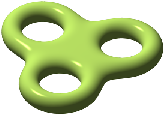
\includegraphics[scale=1.25]{main/Fig02-RiemannSurface}}
\vskip-15pt
\caption{A Riemann surface of genus 3.
\marginparhere{\redden{call in text?}}
}
\label{RiemannSurface}
\end{figure}


\begin{fact} (Hodge theory)
The sole topological invariant of a smooth projective curve $C$,
viewed as an analytic space, is its genus. As a manifold it is a
compact, oriented surface, and its genus is half the rank of its first
singular cohomology, $H^{1}(C; \CC)$, which is equal to its first 
de Rham 
cohomology.
Breaking up the de Rham cohomology of any smooth projective complex variety $X$ in terms of holomorphic and antiholomorphic differential
forms we get the \emph{Hodge decomposition}
$$
H^i(X,\CC) = H^i_{\mathrm{de\,Rham}}(X) = 
\tsty\bigoplus\limits_{j=0}^i H^j(\mwedge^{i-j} \Omega_X).
$$
For a smooth curve $C$, this says in  particular that
$$
H^1(C; \CC) = H^0(\omega_C)\oplus H^1(\sO_C) = H^0(\omega_C)\oplus (H^0(\omega_C))^\vee, 
$$
so $ h^0(\omega_C)$ is half the rank of the middle singular cohomology
group, justifying the name ``genus''. For details, 
see~\cite[p.\,116]{Griffiths-Harris1978}.
\end{fact}

A divisor $E$
of negative degree 
satisfies the equation
$H^0(E) = 0$,
so we get the form of the Riemann--Roch theorem
originally proved by 
\blue{Riemann:}
\index{Riemann, Georg}%

\begin{corollary}\label{nonspecial RR}
For any divisor $D$ of degree $d$ we have
$$
h^0(D) \geq d - g + 1,
$$
with equality if $d > 2g-2$.
\end{corollary}
%
It was 
\blue{Gustav Roch,}
\index{Roch!Gustav}%
a student of
Riemann's, 
who supplied the correction term $h^0(K_C - D)$ for divisors of lower degree.
The dimension $h^0(K_C-D) = h^1(D)$ was called the 
\blue{\emph{superabundance}}
\index{superabundance}%
of $D$: the ``expected'' number of sections was $d-g+1$, and $h^1(\cL)$ reflected how much larger the actual number was.

Corollary~\ref{nonspecial RR} and Proposition~\ref{very ample} together show that all high degree divisors come from hyperplane sections in 
suitable embeddings; and unlike the general vanishing theorems, they give a bound on the degree necessary for vanishing
of cohomology and for
global generation:

\begin{corollary}\label{degree 2g+1 embedding}
Let $D$ be a divisor of degree $d$ on a smooth, connected projective curve of genus $g$.
\begin{enumerate}
 \item If $d>2g-2$ then $H^1(\sO_C(D)) = 0$.
 \item If $d \geq 2g$ then $\sO_C(D)$ is generated by global sections; that is, the complete linear series $|D|$ is basepoint free; and $\sO_C(D)$ is very ample unless $D = K_{C}+E$ for some divisor $E$ of degree 2.
 \item If $d \geq 2g+1$ then $\sO_C(D)$ is very ample; that is, the associated morphism $\phi_D : C \to \PP^{d-g}$ is an embedding, and
$D$ is the preimage of the intersection of $C$ with a hyperplane in $ \PP^{d-g}$.
\end{enumerate}
\end{corollary}

\begin{proof}
If $d>2g-2$ then $K-D$ has negative degree, and thus 
$$h^1(D) = h^0(K-D) = 0. $$ 
The last two parts follow
from the Riemann--Roch theorem and Proposition~\ref{very ample}.
\end{proof}

Since the complement of a hyperplane in projective space is an affine space, we get an affine embedding result too:

\begin{corollary}
 If $C$ is any smooth projective curve and $\Gamma \subset C$ a nonempty finite subset then $C \setminus \Gamma$ is affine (that
 is, isomorphic to a closed subscheme of an affine space).
\marginpar{moved period past parens}     
\end{corollary}

\begin{proof}
Let $D$ be the divisor defined by $\Gamma$. By Corollary~\ref{degree 2g+1 embedding} a high multiple of $D$ is very ample,
and gives an embedding $\phi: C\to \PP^n$ such that the preimage of the intersection of $C$ with some hyperplane $H$
is a multiple of $D$. It follows that $C\setminus \Gamma$ is embedded in $\AA^n = \PP^n\setminus H$.
\end{proof}
 
We can  use Corollary~\ref{nonspecial RR} to determine the Hilbert polynomial of a projective curve. To do this, let $C \subset \PP^r$ be a smooth curve of degree $d$ and genus $g$, and consider the exact sequence of sheaves
$$
0 \to \cI_{C/\PP^r}(m) \to \cO_{\PP^r}(m) \to \cO_C(m) \to 0
$$
and the corresponding exact sequence
$$
 H^0(\cO_{\PP^r}(m)) \ruto{\rho_m} H^0(\cO_C(m)) \to H^1(\cI_{C/\PP^r}(m)) \to 0.
$$

The  $h_C$ of $C$  is defined in terms of the
\blue{\emph{Hilbert function}}
\index{Hilbert function}%
homogeneous coordinate ring $R_{C}$ of $C$ by
\marginpar{removed colon}
$$
h_C(m) = \dim_{\CC} (R_{C})_{m} = \rank \rho_m,
\marginparhere{removed parentheses around argument of rank}
$$
where $(R_{C})_{m}$ is the degree $m$ component of the homogeneous coordinate ring of $C$ in $\PP^n` `$.

By Theorem~\ref{Serre--Grothendieck vanishing} we have
$H^1(\cI_{C/\PP^r}(m)) = 0$ for large $m$.
\redden{Therefore}
\marginpar{to allow line break}
$h_{C}(m) = h^0(\cO_C(m))$ for large $m$, which, by 
\redden{Riemann--Roch}, equals $dm-g+1$, again for large $m$. 
Thus, the Hilbert polynomial of $C \subset \PP^r$ is $p_C(m) = dm-g+1$.  
More generally, we define what is called the \emph{arithmetic genus}:

\begin{definition}\label{genus Hilbert}\label{pa}\label{genus formula}
If $C\subset \PP^n$ is a 1-dimensional projective scheme with Hilbert polynomial
$p_C(m) = \chi(\sO_C(m))$, the \emph{arithmetic genus} of $p_a(C)$ is $1-\chi(\sO_{C}) = 1-p_C(0)$. If $C$ is reduced and irreducible, then
the \emph{geometric genus} $g(C)$ is the genus of the normalization of $C$.
\end{definition}

We see from the Riemann--Roch theorem that if $C$ is smooth and connected, then $p_a(C) = g(C) = h^0(\omega_C)$, the genus of $C$. We
will see that for reduced and irreducible curves $p_a(C) \geq g(C)$, with equality only when $C$ is smooth.
  For some examples with curves that are not
reduced and irreducible, see Exercise~\ref{pa example}.
  

The Riemann--Roch theorem and Serre duality have extensions to arbitrary coherent sheaves in place of invertible sheaves 
and to singular curves, which we will explain in Chapter~\ref{LinkageChapter}.

Divisors $D$ for which $h^0(K_C - D)>0$ are called \emph{special divisors}. The existence or nonexistence of divisors $D$ with given $h^{0}(D)$ and $h^{1}(D)$ often serves to distinguish one curve from another, and will be an important part of our study.

\subsection*{Residues, and a complex analytic argument for 
the Riemann--Roch theorem} 

The 
\marginpar{\vskip-35pt \hskip-14pt{\Large$\downarrow$} the hyphen in ``theorem'' is ugly, but I've been unable to fix it. Perhaps drop ``the'' and ``theorem'' around RR? It will lighten up the section title.\\[4pt]dropped ``as well'' after red text.}
Rie\-mann--Roch theorem is so central to the study of curves that it is worth understanding from another point
\redden{of view.}
We remarked at the beginning of Chapter~\ref{linear series} that a
smooth projective curve over $\CC$ is the same thing as a compact
Riemann surface. 
\redden{Here we will briefly adopt}
the complex analytic viewpoint, and give an explanation of 
\index{complex analytic viewpoint}%
\marginpar{\hskip-50pt $\leftarrow$ streamlined; also removed hyphen in ``complex analytic'' in
  section header to agree with this instance and Chapter 1}
a special case of Theorem~\ref{RR theorem}.

If $D = \sum a_ip_i$ is an effective divisor 
\marginpar{new paragraph}
on a compact Riemann surface $X$ then we write $L(D)$ 
for the vector space of meromorphic functions on $X$ with poles of order 
\marginpar{$\leq\,\to$ at most}
at most $a_i$ at $p_i$. 

\begin{theorem}
Let $X$ be a compact Riemann surface of genus $g$, and let $D$ be an effective divisor of degree $d$ on $X$. Suppose that $K-D$ is also effective for some canonical divisor $K$.
The dimension of  $L(D)$ is
$d-g+1+\dim_\CC L(K-D)$.
\end{theorem}
% avoid double skip
Because  meromorphic functions on a Riemann surface are rational functions on the corresponding
algebraic curve, and $L(D) = H^0(\sO_C(D))$, the assertion is equivalent to Theorem~\ref{RR theorem}.

\begin{proof}
% We will prove this using residues, under the additional assumption that  $D$ and $K-D$ are both effective (that is, $D$ is both effective and \emph{special} in the sense that there are nonzero functions
%both in $L(D)$ and in $L(K-D)$.)
%
Recall that the 
\blue{\emph{residue}} 
of a meromorphic 1-form $\phi$ at a
\index{residue}%
point $p$ on $X$ is defined by an integral: choose a disc $\Delta \subset X$ containing $p$ and in which $\phi$ is holomorphic except
\marginpar{replaced \{\string\rm\ res\} by \string\Res\ (defined with \string\operatorname\string) for the reasons explained in my email to the AMS}
for its pole at $p$. The residue $\Res_p(\phi)$ is $\sfrac{1}{2\pi i}$
times the integral of $\phi$ along the boundary of $\Delta$. If $z$ is
a local coordinate on $\Delta$ zero at $p$ and we write the
differential $\phi$ as
{\meshing
$$
\phi = \sum_{i=-n}^\infty \!a_iz^i \,dz
$$
then by Cauchy's formula, the residue of $\phi$ at $p$ is the coefficient $a_{-1}$. 
}

\begin{proposition}\label{residue sum}
 If $\phi$ is a meromorphic differential on a compact Riemann surface $X$, then the sum of the residues of $\phi$
 at all the poles of $\phi$ is $0$.
\marginpar{made 0 upright, ok?}
 \end{proposition}
 
\begin{proof}
Apply 
\blue{Stokes' theorem}
\index{Stokes' theorem}%
to the complement of the union of small discs around each of the poles of $\phi$.
\end{proof}

Let  $D = \sum a_ip_i$ be an effective divisor on $X$, and set $d = \sum a_i = \deg D$. Locally, a function with a pole of order at most $n$ at $p$ may be written in terms of a local coordinate $z$ at $p$ as $\sum_{i=-n}^\infty a_{i}z^{i} $;
the sum $\sum_{i=-n}^{-1} a_{i}z^{i}$ is called its \emph{polar part}.
By the maximum principle, a meromorphic function in $L(D)$ is determined, up to the addition of a constant, by its polar parts at the points~$p_i$. Thus we have $\dim L(D) \leq d+1$.
{\meshing\par}

When is a given collection $c_1,\dots,c_d \in \CC[z^{-1}]$ the polar parts of a global meromorphic function $f$ on $X$? A necessary condition
is that if $\phi \in L(K)$ is a holomorphic differential on $X$, then
$$
\sum \Res_{p_i}(f \cdot \phi) = 0.
$$
This gives $g$ linear relations on the $c_i$. However, if $\phi$ is a holomorphic differential vanishing at all the points $p_i$
then the corresponding relation is trivial. Thus the number of linearly independent relations on the polar parts of $f$ is actually $g - \dim L(K-D)$; and we arrive at an inequality
$$
\dim L(D) \leq d + 1 - g + \dim L(K-D).
$$

This is a priori only an inequality. But we can apply the same logic to an effective divisor $K-D$, and we see that
\begin{align*}
\dim L(K-D) &\leq \deg(K-D) + 1 - g + L(K - (K-D)) \\
& = 2g - 2 - d + 1 - g  + L(D) \\
&= g - d - 1 + L(D).
\end{align*}
Adding the two inequalities we have
\marginpar{\vskip-20pt added period}
$$
L(D) + L(K-D) \leq L(D) + L(K-D).
$$
Since the sum of the inequalities is an equality, we conclude that each inequality is also an equality; this is the Riemann--Roch formula
in our special case.
\end{proof}

\subsection*{Arithmetic genus and geometric genus}

Throughout this book, we will be primarily concerned with the geometry of smooth curves. Of course singular curves will arise\emdash for example, as images of smooth curves under morphisms that are not embeddings. At least when $C$ is a 1-dimensional variety (that is, a 
reduced irreducible 1-dimensional scheme) we can  regard $C$ as the image of a smooth curve in an optimal way:
\marginpar{replaced ``(Proposition~\ref{resolution of singularities})'' by colon}

\begin{proposition}\label{resolution of singularities}
If $C_0$ is a projective variety of dimension 1 then the \emph{normalization} $\phi: C \to C_0$ of $C_0$ is a birational
morphism from a smooth curve $C$. The curve $C$ is again projective, and the pair $(C, \phi)$ is
unique up to  isomorphism. In particular, every birational map of smooth curves is an isomorphism.
\end{proposition}
 
\begin{proof}
  We use the result that the normalization ($=$ integral closure) of a domain
finitely generated over a field is again finitely generated, and nonsingular in codimension 1 \cite[Theorem 4.14 and 11.5]{Eisenbud1995}. Thus,
starting with a projective embedding of $C$ we normalize the homogeneous coordinate ring of $C$. The resulting ring
may have generators in many degrees, but a suitable Veronese subring will be generated in a single degree, and thus
is the homogeneous coordinate ring of a smooth projective curve. 

Localization
\marginpar{reworded to avoid unpleasant hyphens}
commutes with normalization, and any map from a normal ring to a
domain factors uniquely through the normalization. 
\redden{Therefore}
the normalization is unique.
\end{proof}

A different, less canonical procedure for finding a smooth curve birational to a given curve
is explained in 
\marginpar{the xref here was undefined; I assume the last 3 exercises are relevant and coded accordingly. Please check}
\redden{Exercises \ref{Veronese of plane curve} to \ref{Mumford resolution argument}}.


Still assuming that $C_0$ is reduced and irreducible, we can relate
\marginpar{it's it obvious what these terms mean?}
\index{arithmetic genus}%
\index{geometric genus}%
\index{genus!arithmetic versus geometric}%
the
\redden{arithmetic and geometric genera}
of $C_0$ using the map of sheaves
$$
\cO_{C_0} \to \nu_*\cO_C.
$$
Since the normalization map of rings  is injective and finite, this map is injective. The cokernel $\sF$ is a coherent sheaf supported on the singular points of $C_0$, and is thus finite over $\CC$. 
The definition implies that there is a short exact sequence
$$
0 \to \cO_{C_0} \to \nu_*\cO_C \to \cF \to 0.
$$

\begin{proposition}\label{pa and delta}
Suppose that $C_{0}$ is a reduced, irreducible curve and let  $\nu: C\to C_{0}$ be its normalization.
Let $\sF = \nu_{*}\sO_{C}/\sO_{C_{0}}$. If we set 
$\delta(C_{0}) := h^{0}(\sF)$, 
\redden{then}
 $$
p_a(C_0) - g(C) =  \delta(C_{0})
$$ 
\end{proposition}

\begin{proof}
 Since the normalization map $\nu: C \to C_0$ is finite,  the direct images $R^i\nu_*\cO_C$ vanish for $i > 0$, 
so the Leray spectral sequence 
\redden{(see \ref{Leray} just below)}
computes $\chi(\nu_*\cO_C) = \chi(\cO_C)$. Thus
$$
p_a(C_0) - g(C) =  \chi(\cO_{C}) -   \chi(\cO_{C_0}) = \chi(\cF) = h^0(\cF) 
$$ 
since the support of $\cF$ is finite.
\end{proof}

The operation of normalization localizes, so we can understand $\sF$ by looking at it locally.
Writing $R$ for the affine ring of some affine subset $U\subset C_{0}$ we see that $\sO_{C}|_{U}$
is the integral closure $\ovR$ of $R$, so $\sF|_{U}$ is $\ovR/R$. Thus
the annihilator of $\sF|_{U}$, called the \emph{conductor}
$\ff_{\ovR/R}$,
\marginpar{added comma before red phrase}
\redden{is an ideal of both $\ovR$ and $R$,}
and correspondingly $\nu^{-1}(\ff_{C/C_{0}})$ 
is also an ideal sheaf in $\sO_{C}$.

Informally, we may say that $\delta(C_{0})$ is the number of linear
conditions a locally defined function $f$ on $C$ has to satisfy to be
the pullback of a function from $C_0$. The length of the stalk of
$\cF$ at a particular singular point $p \in C_0$ is called the
\index{delta invariant|$\delta$-invariant}
\emph{$\delta$-invariant} $\delta_p$ of the singularity. Thus 
\marginpar{semicolon $\to$ colon; added punctuation in display}
$$
p_a(C_0) - g(C) = \sum_{p @\in@ (C_0)_{\mathrm{sing}}\!\!} \delta_p.
$$ 

\begin{fact}~\label{Leray}
 In general, the 
\blue{Leray spectral sequence}
\index{Leray spectral sequence}%
addresses the situation of  a morphism $f:X\to Y$ of varieties or schemes, 
 and a coherent sheaf $\sG$  on the source $X$; it says in this circumstance that there is a spectral sequence
  $$
  \HH^p(R^qf_*(\sG)) \Longrightarrow \HH^{p+q}(\sG).
  $$
(This is a special case of the spectral sequence for the derived functors of a composite functor ($H^0$ composed with $f_*$);
see~\cite[II.4.17.1]{Godement} or \cite[Section III.7]{Gelfand-Manin} for proofs.)
\end{fact}

In the simplest cases the $\delta$ invariant is easy to compute:


\begin{enumerate}

\item A 
\index{node}%
\blue{\emph{node}}
of a curve $C_0$ is a point $p$ such that
\marginpar{removed ``(nodes)''}
  an analytic neighborhood of $p$ in $C_0$ consists of two smooth arcs
  intersecting transversely at $p$ 
\redden{(See Figure \ref{simplesing}, left.)}
Equivalently, the completion of
  the local ring $\cO_{C_0,p}$ is isomorphic to $k\[x,y\]/(xy)$. If $p
  \in C_0$ is a node, its preimage in the normalization $C$ of $C_0$
  consists of two points $r,s\in C$. The condition for a function $f$
  on $C$ to descend to $C_0$\emdash that is, to be the pullback of a function
on $C_0$\emdash is  that $f(r)=f(s)$; this is one 
linear condition, so $\delta_p = 1$.

\item  
\redden{A}
\index{cusp!ordinary}%
\blue{\emph{cusp}} 
\marginpar{I'm reacting here to the ``(cusps)'' in parens in the versus the term actually defined.}
\redden{(strictly speaking, an \emph{ordinary cusp})}
of a curve $C_0$ is a point $p$
  such that an analytic neighborhood of $p$ in $C_0$ is given by the
  equation $y^2=x^3` `$. 
\redden{(See Figure \ref{simplesing}, second from left.)}
If $p \in C_0$ is an ordinary cusp then its
  preimage in the normalization $C$ of $C_0$ will consist of one point
  $r\in C$. The condition for a function $f$ on $C$  is that the
  derivative $f'(r)=0$; again, this is one linear condition, so
  $\delta_p = 1$. 
\marginpar{moved \string\end\{enumerate\} so the break appears before ``We will''}
\end{enumerate}

We will give more examples at the end of
Chapter~\ref{PlaneCurvesChapter}.



\begin{figure}   % appears as 2.4
\centerline{%
  \includegraphics[height=2in]{"main/Fig02-sing-node"}\hfil\quad
  \includegraphics[height=2in]{"main/Fig02-sing-cusp"}\hfil\quad
  \includegraphics[height=2in]{"main/Fig02-sing-tacnode"}\hfil\quad
  \includegraphics[height=2in]{"main/Fig02-sing-triple"}}
\caption{Simple planar curve singularities.
\index{tacnode}%
\index{triple point}%
\index{planar curve singularities}%
\index{singularity!of planar curve}%
\label{simplesing}
}
\end{figure}


\section{The canonical morphism}

We now return to the world of smooth curves.
\index{canonical morphism}\index{morphism!canonical}%

 The canonical sheaf on $\PP^1$ has negative degree, so $|K_{\PP^1}| = \emptyset$. If $C$ is a curve
 of genus $1$ then the canonical sheaf     has a nonzero global section, and since the sheaf has degree $2g-2=0$ this is nowhere vanishing, whence
 $\omega_C = \sO_C$, and $K_C = 0$. Thus in studying the canonical series we restrict our attention to curves $C$ of genus $g\geq 2$. 
 
 \begin{theorem}\label{canonical series is very ample} Let $C$ be a smooth curve of genus $\geq 2$.
\begin{enumerate}
 \item $|K_C|$ is basepoint free.
 \item $|K_C|$ is very ample if and only if $C$ admits no map of degree 2 to $\PP^1` `$.
\end{enumerate}
\end{theorem}

A curve of genus $\geq 2$
is said to be \emph{hyperelliptic} if there exists a 
\blue{morphism}
$f: C \to \PP^1$ 
\begingroup\def\marginpar#1{}%
\blue{of degree 2.}
\endgroup
\index{hyperelliptic}%
\index{morphism!of degree 2}%
It is easy to describe this in terms of linear series:

\begin{lemma}\label{deg 2 morphism}
Let $C$ be a smooth, projective curve of genus $g\geq 2$. If $C$ has an invertible sheaf $\cL$ of degree $\leq 2$ with two independent sections, then $\cL$ has degree~$2$ and
$|\cL|$ defines a morphism of degree $2$ to $\PP^{1}$, so $C$ is
hyperelliptic. In particular, if $g(C) = 2$ then the canonical series
\marginpar{hyphenated 2-to-1 (and uprighted digits in statements) to agree with the math occurrences}
$|K_{C}|$ defines a $2$-to-$1$ morphism to $\PP^{1}$, so $C$ is
hyperelliptic.
\end{lemma}

\begin{proof}
Since $C \not\cong \PP^1` `$,  Theorem~\ref{characterization of P1} shows that $C$ cannot have a 1-dimensional linear series
of degree $< 2$. Thus $\sL$ has degree exactly 2, and no 
\marginpar{\redden{You defined ``base point'' in chapter 1; this must be the same thing, but here you're writing it as one word. Either is fine, but we should be consistent.  I lean toward no space, since ``base point free'', ``base-point free'' or ``base-point-free'' are all awkward. But it's up to you.}}
\redden{basepoints,}
so it defines a morphism of degree 2 to $\PP^1$ as claimed.
\end{proof}

\begin{proof}[Proof of Theorem~\ref{canonical series is very ample}]
A point $p$ is a basepoint of $|K_C|$ if and only if 
\marginpar{displayed to allow line break}/that
$$h^0(K_C-p) = h^0(K_C) = g.$$ 
By the Riemann--Roch theorem,
this is eqivalent to $h^0(p) =2$, which would imply that $C\cong \PP^1$ by Theorem~\ref{characterization of P1}. Thus $K_C$
has no basepoints.

By Proposition~\ref{very ample} we 
\redden{must}
show that for any 
\redden{two}
points $p, q \in C$ we have
\unskip\marginpar{for better layout}
$$
h^0(K_C(-p-q)) = h^0(K_C)-2 = g-2.
$$
Applying the Riemann--Roch theorem we see 
\marginpar{added ``that'' to allow line break}
that this fails if and only if $h^0(\cO_C(p+q)) \geq 2$ for some $p,q
\in C$. By Lemma~\ref{deg 2 morphism}, this implies that $C$ is
hyperelliptic. Conversely, if $C$ is hyperelliptic then for some
divisor $D = p+q$ we have $h^0(D) = 2$, whence $h^0(K-p-q) = h^0(K)
-1$ by 
the Riemann--Roch formula.
\emergencystretch5.5pt
\end{proof}

The image of the canonical morphism of a nonhyperelliptic curve of
genus $g>2$ is called a 
\blue{\emph{canonical curve},}
\index{canonical curve}%
and (for a nonhyperelliptic curve) we  
speak of the image as being \emph{canonically embedded}.


\subsection*{Geometric Riemann--Roch}

There is a useful way of expressing the Riemann--Roch formula in terms
of the geometry of the canonical map. Suppose $C \subset \PP^r$ is a
smooth curve and $D$ an effective divisor on $C$, thought of as a
subscheme of $C$. We define the 
\blue{\emph{span}}
\index{span!of effective divisor}%
$\ovD$ of $D$ to be the
\marginpar{the index entry is ``span of effective divisor; this covers $\overline{\phi(D)}$ as well, right?}
intersection of the hyperplanes $H \subset \PP^r$ containing $D$. More
generally, if $\phi : C \to \PP^r$ is a map and $D$ an effective
divisor on $C$, we define the span $\overline{\phi(D)} \subset \PP^r$
to be the intersection 
$$
\overline{\phi(D)} := \bigcap_{ 
\substack{H \subset \PP^r \text{ a hyperplane} \\D \subset
  \phi^{-1}(H)}}
H.
\marginparhere{stacked conditions to avoid superwide subscript, ok?}
$$

Now suppose $C$ is a smooth curve of genus $g\geq 2$ and $\phi_K: C\to \PP^{g-1}$ is the canonical morphism.
If  $D$ is an effective divisor on $C$ of degree $d$, then since the hyperplanes in $\PP^{g-1}$ containing $\phi_K(D)$ correspond (up to scalars) to sections of $K_C$ vanishing on $D$, we see that
$$
h^0(K_C-D) = \codim \overline{ \phi_K(D)} \subset \PP^{g-1}= g - 1 - \dim \overline{ \phi_K(D)}.
$$
\index{geometric!Riemann--Roch theorem}%
\index{Riemann--Roch theorem!geometric}%
Applying the Riemann--Roch theorem we obtain  the \emph{geometric Riemann--Roch theorem}:

\begin{corollary}\label{geometric RR}
If $D$ is a divisor on a smooth curve $C$ of genus $\geq 2$ then
$$
r(D) = d - 1 - \dim \overline{ \phi_K(D)}.
\vspace*{-3pt}
$$
\end{corollary}
%
In particular, if $D = \sum_{i=1}^dp_i$ is a sum of distinct points, then
 the dimension of the linear series $|D|$  is equal to the number of linear relations among the images of the $p_i$ on the canonical 
 image of $C$. 
 Thus, for example, a divisor given as the sum $D = p+q+r$ of three
 points will move in a pencil if and only if the three points are
\marginpar{\hskip-100pt $\leftarrow$ colinear $\to$ collinear (there were about equal numbers of each, I uniformized toward the old-fashioned spelling, ok?\\[3pt] streamlined passage in red; original had $\mathrm{p}_{\mathrm{a}})$, but that  seems to have been a coding error}
 collinear on the canonical model. 

In general, 
the condition on forms of degree $d$ to vanish at 
\redden{a given point $p$ in $\PP^r$ is expressed}
by one homogeneous linear
 linear equation on the coefficients of the form, obtained by evaluating the variables at 
 the coordinates of $p$, so vanishing on a set $\Gamma$ of $\gamma$ points is given by
 $\gamma$ linear equations and the same is true when $\Gamma$ is a finite subscheme
 of length $\gamma$, as one sees from the exact sequence
 $$
 0\to H^0(\sI_\Gamma(d) \to H^0(\sO_{\PP^r}(d)) \ruto{ev} H^0(\sO_{\Gamma}(d)) \to 0,
 $$
 bearing in mind that 
 $$
 H^0(\sO_{\Gamma}(d)) \cong H^0(\sO_{\Gamma}) \cong \CC^\gamma.
 $$
However, the linear equations may be linearly dependent; that is, the map marked $ev$
above may have rank $<\gamma$. We will say that the points of $\Gamma$
\emph{fail to impose independent conditions on hypersurfaces of degree $d$}
by the amount equal to $\gamma - \rank(ev)$. 

With this terminology, the geometric Riemann--Roch theorem says that 
the dimension of the complete linear series $|D|$ on a smooth curve $C$
is the amount by which the points of $D$ fail to impose independent conditions
on canonical divisors, and the geometric version simply translates this into 
 hyperplanes in the canonical embedding of $C$. 
\index{Cayley--Bacharach--Macaulay theorem}%
The Cayley--Bacharach--Macaulay
theorem~\ref{CBM} and the result of 
\marginpar{\redden{missing xref `pluricanonical'}}
Exercise~\ref{pluricanonical} are other useful
special cases.

\begin{remark}
For a singular curve $C_0$ to have a canonical morphism it is necessary first of all that its canonical sheaf
 $\omega_{C_0}$ be invertible; when this is the case, we say that $C_0$ is (locally) Gorenstein, and then
\index{locally Gorenstein}%
\index{Gorenstein!locally}%
the theory above can be applied. See for example \cite{graphcurves} and \cite{ribbons} for examples. 
\end{remark}

\subsection*{Linear series on a hyperelliptic curve}
We can describe the canonical map of a hyperelliptic curve\emdash and indeed all its special linear series\emdash quite precisely:

\begin{corollary}\label{canonical on hyperelliptic}
Let $C$ be a smooth hyperelliptic curve of genus $g\geq 2$. The curve $C$ admits a unique degree 2 morphism $\pi: C\to \PP^1` `$,
and the canonical map $\phi_K: C\to \PP^{g-1}$ is the composition of $\pi$ with the Veronese map of degree $g-1$ from
\index{Veronese map}%
$\PP^1$ to the rational normal curve of degree $g-1$; in particular, every canonical divisor is a sum of $g-1$ fibers of $\pi$ and vice versa.
\end{corollary}

\begin{proof}
If $D$ is a general fiber of a degree 2 map $\pi:C\to \PP^1$ so that $D= p+q$ and $r(D) = 1$, then by the Riemann--Roch theorem or its geometric version, $D$ imposes only one condition on sections of $K_C$; that is, $\phi_K(p) = \phi_K(q)$. Consequently the degree of the canonical morphism $\phi_K$ is at least 2, and the image is thus a nondegenerate curve in $\PP^{g-1}$ of degree $\leq (2g-2)/2 = g-1$. By Theorem~\ref{characterization of P1}, the image of $\phi_K$ is the rational normal curve of degree $g-1$ and every fiber of $\phi_K$ is a divisor linearly equivalent to $D$. It follows that $\pi$ is determined by $K$, so it is unique. Since every canonical divisor is the pullback of a hyperplane section of the rational normal curve,
every canonical divisor is a sum of $g-1$ fibers of $\pi$.
\end{proof}

We can use these ideas to analyze all special divisors.
\index{special divisor}%
\index{divisor!special}%

\begin{corollary}\label{special on hyperelliptic} Let $C$ be a smooth 
\blue{hyperelliptic curve}
\index{hyperelliptic curve}%
with map $\pi: C\to \PP^1$ of degree 2.
Every special divisor $D$ of degree $d$ on 
\marginpar{a hyperelliptic curve $\to C$}
$C$ is a sum of $s$ fibers of $\pi$ and $d-2s$ points
$p_1,\dots,p_{d-2s}$ with distinct images under the canonical map; and
in this case we have $r(D) = s$ and the points $p_i$ are base points
of the linear series $|D|$.
\end{corollary}

\redden{Thus}
\emph{no divisor on a hyperelliptic curve is both special and very ample}.
\marginpar{streamlined}

\begin{proof}
Suppose that $D$ contains the sum $E$ of $s$ fibers of $\pi$ and no more; and write $D = E+D'$, with $\deg D' = d-2s$.
 
If $\phi_K:C \to \PP^{g-1}$ is the canonical map, then $\phi_K(D')$ consists of $d-2s$ distinct points, while $\phi_K(E)$ consists of
$s$ points. By Corollary~\ref{independence of points on a RNC} the span of $\phi_K(D)$ has dimension $\min\{g-1, d-s-1\}$, so 
$r(D) = d-1-\min\{g-1, d-s-1\} = \max \{s,d-g\}$. Since $D$ is a special divisor, $r(D) > d-g$, so $r(D) = s$. 
Since $r(E) =s$, we see that $E$ is basepoint free, so $D'$ is the base locus of $D$.
\end{proof}

\section{Clifford's theorem}\label{Clifford Section}

While the Riemann--Roch theorem gives a lower bound for the dimension of a linear series, $r(\sL) := h^0(\sL)-1 \geq \deg \sL -g$, Clifford's theorem
\index{Clifford's theorem}%
gives an upper bound. If $\deg \sL>2g-2$, then the Riemann--Roch
inequality becomes an equality, so it is enough to treat the case
$\deg \sL \leq 2g-2$. The bound is actually a corollary of the 
Riemann--Roch theorem.

\begin{corollary}\label{Clifford bound}
 Let $C$ be a curve of genus $g$ and $\cL$ a line bundle of degree $d \leq 2g-2$. Then
$$
r(\cL) \leq \frac{d}{2}.
$$
\end{corollary}

\begin{proof}
If $\cL$ is nonspecial then, since $g\geq d/2 + 1$, we have $r(\cL) = d-g+1\leq d/2$.
Otherwise we have
$$
r(K_C\otimes \cL^{-1}) = r(\cL) +g - d - 1
$$
by the Riemann--Roch theorem,
and so by Proposition~\ref{sum of linear series}
$$
g = r(K_C)+1  \geq r(\cL) + r(K_C\otimes \cL^{-1}) +1  = 2r(\cL) +g - d;
$$
hence $r(\cL) \leq d/2$.
\end{proof}

The usual statement of Clifford's theorem includes a description of when equality can occur:

\begin{theorem}\label{Clifford}\label{Clifford equality}
Let $C$ be a curve of genus $g$ and $\cL$ a line bundle of degree $d \leq 2g-2$. If
$$
r(\cL) = \frac{d}{2},
$$
the largest possible value, then either
\begin{enumerate}
\item $d=0$ and $\cL = \cO_C@$;
\item $d = 2g-2$ and $\cL = K_C@$; or
\item $C$ is hyperelliptic, and $|\cL|$ is a multiple of the $g^1_2$ on $C$.
\end{enumerate}
\end{theorem}

From Corollary~\ref{canonical on hyperelliptic} and Corollary~\ref{geometric RR} we see that the equality does indeed hold
in each of the cases enumerated. See
Corollary~\ref{equality in Clifford from Martens} for the converse and \cite[IV.5.4]{Hartshorne1977}
for a different proof.

 \section{Curves on surfaces}\label{surface basics}
 
 We will often analyze curves  on a smooth surface. Compared to the theory of linear series on curves, there is a new element: the intersection pairing. We refer to~\cite[Chapter V]{Hartshorne1977}
\index{intersection pairing}%
 and~\cite[Chapter I]{Beauville} for 
\marginpar{``proof'' ok? Or would ``proofs'' be better?}
\redden{proof} 
of the unproven statements in this section.
 We suppose for this section that $S$ is a smooth projective surface,
 and write $\Pic(S)$ for the group of invertible sheaves on $S$.

\subsection*{The intersection pairing}

When two codimension-1 subschemes $D,E$ on $S$ 
\marginpar{upgraded to a subsection (instead of subsub; see also note at top of page 50}
meet transversely we define $D\cdot E$ to be the number of points in which they meet.  
It is less obvious how one might define an intersection number $D\cdot E$ in more general cases,
including the case $D=E$. However 
a codimension-1 subvariety of $S$ has a 
\index{fundamental class}%
fundamental class in $H^{2}(X,\ZZ)$, and the product just defined
agrees with the cup product pairing
\index{cup product pairing}%
$$
H^{2}(S,\ZZ) \times H^{2}(S,\ZZ) \to H^4(S,\ZZ)\cong \ZZ,
$$
showing that it is possible. For example, the self-intersection $D\cdot D$ can be realized geometrically
 by choosing a  vector field $\sigma$ on $D$ and using it to push a copy $D'$ of $D$ infinitesimally away from $D$; then
 one can count the points where $\sigma$ becomes tangent to $D$. Here one must take orientations into account,
 and the result is that $D\cdot D$ may be negative. In the previous case (and when $\sigma$ is complex analytic)
 the multiplicities are all positive because a complex subvariety is canonically oriented using the orientation of $\CC$
 itself.

\begin{figure}   % appears as 2.5
\inprogress
\centerline {\includegraphics[height=1.75in]{"main/Fig02-strip"}}
\captionPlus{Fig02-strip}{The result, $D'$, of moving $D$ infinitesimally along a normal vector field meets $D$ twice.
\marginparhere{\hsize=2.5in\redden{call in text?} Also, this needs redrawing; the arrows are supposed to be perpendicular to the curve, but in perspective they may not look so, since the the supporting surface is not planar, right?}
}
\end{figure}

This pairing can be realized algebraically as follows:

First, if $D$ and $E$ have no common
\index{intersection multiplicity}%
components, then the \emph{intersection multiplicity} 
$m_S(D,E,p)$ at $p\in S$
is defined as the vector space dimension of the local ring $\sO_{S,p}/(\sI_{D,p}+\sI_{E,p})$, and 
$$
D\cdot E = \sum_p m_S(D,E,p).
$$

Quite generally, 
the intersection product can be computed using the (algebraic) Euler
characteristic. 
\marginpar{dropped ``and'' and started new sentence}
\redden{This}
works even for 
\blue{Cartier divisors}
on a singular surface: Setting $\sL := \sO_S(D)$ and
\index{Euler characteristic}%
\index{Cartier divisor}%
$\sM := \sO_S(E)$ to simplify the notation, we have 
$$
D\cdot E = \chi(\sO_S)-\chi(\sL^{-1}) -\chi(\sM^{-1}) +\chi(\sL^{-1}\otimes \sM^{-1}) 
.
$$

\begin{theorem} The pairing $(D,E) \mapsto (D\cdot E)$ is the unique bilinear map
$\Pic(S) \times \Pic(S) \to \ZZ$ extending the case of intersections of two curves meeting transversely at smooth points of $S$. 
\end{theorem}

An important special case is that of the self-intersection $D\cdot D = D^2` `$. The general formula reduces immediately to the case of an effective divisor, and in that case it resembles the $C^{\infty}$ construction above:

\begin{corollary}\label{self-intersection number}
If $D$ is a codimension $1$ subscheme of $S$, then the self-intersection $D\cdot D$ is the degree of the normal bundle
$\sN_{D/S} := \sO_{D}(D)$.
\end{corollary}

\begin{proof}
Substituting $\sO_{S}(-D)$ for both $\sL^{-1}$ and $\sM^{-1}$ we
\redden{have the}
\marginpar{streamlined and undisplayed sequences for better layout}
%compute from the short 
exact sequences
\begingroup
\thickmuskip = 4.5mu plus 1mu 
$ 0\to \sO_{S}(-D)\to \sO_{S}\to \sO_{D}\to 0@$ and 
$@0\to \sO_{S}(-2D)\to \sO_{S}(-D)\to \sO_{D}(-D)\to 0$;
the Riemann--Roch theorem 
\endgroup
\redden{then gives}
\begin{align*}
\chi(\sO_{S}) -\chi(\sO_{S}(-D)) &= \chi(\sO_{D}) = -p_{a}(D) +1,\\
\chi(\sO_{S}(-D)) -\chi(\sO_{S}(-2D)) &= \chi(\sO_{D}(-D)) = -\deg \sO_{D}(D) - p_{a}(D) +1.
\end{align*}
Subtracting the second of these equations from the first we see that
$D\cdot D = \deg \sO_{D}(D)$.
\end{proof}

Using the intersection pairing we can turn the adjunction formula of Proposition~\ref{adjunction} into a numerical formula:

\begin{theorem}[adjunction formula]\label{adjunction formula} 
If $C$ is a Cartier divisor on a smooth surface $S$ then
\index{adjunction formula}%
$$
p_a(C) = \frac{(K_X+C)\cdot C}{2} +1.
 $$
\end{theorem}

\subsection*{The Riemann--Roch theorem for smooth surfaces}
Often we wish to compute the dimension of the space of sections of an invertible sheaf, but
\marginpar{\redden{The section ``Curves on surfaces'' had three subsections: a long one on curves on quadrics, and two shorter ones.  As they seemed independent, I've placed the shorter ones first, and made the one on quadrics into a section (2G) instead of a subsection.}}
as with the case of curves, the Euler characteristic is more accessible:

\begin{theorem}[Riemann--Roch for surfaces] Let $\sL$ be an invertible sheaf on a smooth surface $S$.
\index{Riemann--Roch theorem!for surfaces}%
\index{Euler characteristic}%
The Euler characteristic $\chi(D) := h^0(\sL)-h^1(\sL)+h^2(\sL)$, where $\sL = \sO_S(D)$, is given by
$$
\chi(D) = \chi(\sO_S) + \frac{(D-K_S)\cdot D}{2}+1
.
\marginparhere{added punctuation in these and some other displays}
$$
\end{theorem}

\subsection*{Blowups of smooth surfaces}

It is useful to know what happens under mappings of surfaces, particularly the case of the mapping
\index{blowup!of smooth surface}
corresponding to blowing up a point.

\begin{theorem}\label{divisor classes on blowup}
If $\pi: X \to Y$ is a birational map of smooth surfaces, then the pullback map on divisors
preserves the intersection pairing. If $X$ is the blowup of~$Y$ at a point $p$ with exceptional
divisor $E = \pi^{-1}(p)$, then:

\begin{enumerate}
 \item $\Pic X =\pi^*(\Pic Y) \oplus \ZZ E$.
\item The canonical class on $X$ is given by $K_X = \pi^*(K_Y)+E$.
 \item The intersection pairing on $\Pic X$ is given by:
 
\begin{itemize}
\item $\pi^*(D)\cdot\pi^*(D') = D\cdot D'$ for all $D,D'\in \Pic Y$.
\item $\pi^*(D)\cdot E = 0$ for all $D\in \Pic Y$.
 \item $E\cdot E = -1$.
 \item $K_X\cdot E = -1$.
 \item If $C$ is a curve that has an $m$-fold point at $p$ then
   $\pi^{-1}(C)$ contains $E$ with multiplicity $m$, so that the 
\index{proper transform}
proper transform
 $\tilde C$\emdash that is, the closure in $X$ of the preimage of $C \setminus \{p\}$\emdash has class
 $$
 \tilde C \sim \pi^*C - mE.
 $$
 \end{itemize}
\end{enumerate}
\end{theorem}

Using these facts, we can compare the adjunction formula applied to a curve $C$ on a smooth surface $S$ to the formula applied to the proper transform $\tilde C \subset \tilde S$: we have
$$
\tilde C \cdot \tilde C = C \cdot C - m^2 \quad \text{and} \quad \tilde C \cdot K_{\tilde S} = C \cdot K_S + m.
$$
Combining these, we arrive at the formula
$$
p_a(\tilde C) = p_a(C) - \mbinom{m}{2},
$$
and thus the $\delta$-invariant of $p \in C$ is $\tbinom{m}{2}$ plus the sum of the $\delta$-invariants of all the 
points of $\tilde C$ in the preimage of $p$. One can resolve the curve singularity by repeatedly blowing up in this way and thus compute the $\delta$-invariant
of any singularity as a sum of binomial coefficients.

In the special case where $\tilde C$ is smooth\emdash for example, if
the point $p \in C$ is an \emph{ordinary $m$-fold point}, consisting
\marginpar{\redden{what should ``ordinary $m$-fold point'' be indexed under}}%
\index{ordinary $m$-fold point}%
of $m$ smooth branches with distinct tangent lines\emdash we conclude
that the $\delta$-invariant of the point $p$ is $\tbinom{m}{2}$. 


Blowups occur frequently in the theory of surfaces, and are
\index{Castelnuovo's theorem}%
characterized by \emph{Castelnuovo's theorem} 
\cite[Theorem V.5.7]{Hartshorne1977}. 

\begin{theorem}
If $E\subset X$ is a curve on a smooth projective surface $X$ and
\index{blow-down}%
 that $E^2 = E\cdot K_X = -1$ then $E$ can be ``blown down'' in the sense that
 $X$ is the blowup of a smooth surface $Y$ at a point $p\in Y$, and $E$ is the exceptional divisor.
\end{theorem}




\section{Quadrics in $\PP^3$ and the curves they contain}
\label{Div of quadric}
 
 We will frequently be interested in curves on a quadric surface in $\PP^3` `$, and we can describe these
curves and their intersections very concretely.

\subsection*{The classification of quadrics} The form defining a quadric $Q\subset \PP^{3}$ can be written in suitable
\index{classification of quadrics}\index{quadric!classification of --s}%
coordinates $x_{i}$ as 
$$q = \sum_{i=0}^{3} x_{i}^{2},$$ 
where $r\leq 4$ is the \emph{rank} of $Q$. (The corresponding
statement is also true in $\PP^{r}$, with $m\leq r+1$.) Equivalently, this is the rank of the symmetric matrix $M$
representing the bilinear form $\frac12(q(x+y)-q(x)-q(y))$.

\begin{enumerate}
\item A quadric of rank 1 is a double plane.
\index{double plane}%
\marginpar{changed to \{enumerate\} for ease of reference to the result in (d)}
\item A quadric of rank 2 is the union of two distinct planes. 
\item A quadric $Q$ of rank 3 is a cone over a smooth plane conic. The cone point is called the vertex. Every line
\index{vertex}%
on such a quadric passes through the vertex. The 
\blue{Picard group}
\index{Picard group}
of $Q$ is $\ZZ$
\cite[Exercise II.6.5]{Hartshorne1977}.
\marginpar{removed parens around cite}

\item A quadric $Q$ of rank 4 is smooth and is isomorphic to
  $\PP^{1}\times \PP^{1} \subset \PP^{3}$, embedded by the Segre
  embedding. Every line on such a quadric has the form $\PP^{1}\times
  \{p\}$ or $\{p\} \times \PP^{1}$; the two families of such lines are
  called 
\blue{\emph{rulings}.}
\index{ruling}%
\index{Segre embedding}%
\label{smooth quadric}
The Picard group of $Q$ is $\ZZ\times \ZZ$, generated by the lines of the rulings.
\cite[Example II.6.1]{Hartshorne1977}.
\marginpar{removed unmatched right parens}

\item Quadrics in $\PP^{r}$: Inside the space $\PP(\sO_{\PP^{r}}(2)) = \PP^{\binom{r+2}{2}-1}$ the space
of singular quadrics is a hypersurface of degree $r+1$, called the \emph{discriminant}, which is defined by the determinant of a generic symmetric
\index{discriminant}%
$(r+1)\times (r+1)$ matrix $M$. More generally, the rank $k$ locus is defined by the $(k+1)\times (k+1)$
minors of $M$.
\end{enumerate}

%\subsection*{Curves on quadrics}

\redden{It follows that}
\marginpar{\redden{the \{itemize\} here wasn't a coherent list. The first item became this paragraph and the next two became examples, because in an exercise, you referred to one of them as Example~(section number).}}
an irreducible nondegenerate  curve cannot be contained in a quadric of rank 1 or 2.

\subsection*{Some classes of curves on quadrics}

\begin{example}
Let $C$ be a reduced curve on a quadric $Q$ of rank 3 in $\PP^{3}$. 
If $C$ has even degree $2m$ then $C$ is a complete intersection
of the quadric with a hypersurface of degree $m$. Therefore if the curve is smooth it cannot contain the vertex of the quadric. The genus of $C$ is $(m-1)^{2}$.

If $C$ has odd degree $2m+1$, then the union of $C$ with a line on the quadric has even degree,
so if $L_{1}, L_{2}$ are lines on the quadric, then 
$$
C\cup L_{1} = Q\cap F_{1} \quad\hbox{and}\quad C\cup L_{2} = Q\cap F_{2}
$$
are complete intersections of $Q$ with forms of degree $m+1$, and the homogeneous ideal of $C$ is generated by the equations
of $Q,F_{1}$ and $F_{2}$. The genus of $C$ is $m(m-1)$. The curve $C$ contains the vertex, and is a 
\index{Weil divisor}%
\index{Cartier divisor}%
Weil divisor, not a Cartier divisor. These things follow from the description of the desingularization
of $Q$ in Corollary~\ref{singular scrolls}.
\end{example}

\begin{example}
\label{curves on quadrics}
If $C$ is a reduced curve on a quadric $Q$ of rank 4, then in terms of the isomorphism
$Q \cong \PP^{1}\times \PP^{1}$ we can express the divisor class of $C$ as $(a,b)\in \Pic(Q) = \ZZ\oplus \ZZ$.
The intersection form on $Q$ is determined by the fact that the lines of a ruling are all linearly equivalent,
so that $(1,0)^{2} = (0,1)^2=0$ and $(1,0)\cdot (0,1) = 1$; thus $(a,b)\cdot (d,e) = ae+bd$. The hyperplane section
has class $(1,1)$, and the canonical class is $(K_{\PP^{3}}+Q)\mid_{Q} = (-2,-2)$ by the adjunction formula. 

Thus
if $C$ has class $(a,b)$ then the degree of $C$ is $a+b$, while the genus of $C$ is $(a-1)(b-1)$. Note that 
if  $a =b$, the curve is a complete intersection, and if $b = a+1$ then the curve is residual to
a line in a complete intersection of the quadric with a surface of degree $b$. In these cases we get the same genus and degree as we would for a curve
on a rank 3 quadric.


The cohomology of $\sO_{Q}(a,b)$ is determined by the K\"unneth formula
\index{K\"unneth formula}%
\index{Leray spectral sequence}%
(or the Leray spectral sequence) as
$$
H^{i}(\sO_{Q}(a,b)) = \tsty\bigoplus\limits_{i = s+t}H^{s}
(\sO_{\PP^{1}}(a))\otimes H^{t}(\sO_{\PP^{1}}(b)).
$$
The degrees of the generators of the homogeneous ideal of $C$ can be determined from the exact sequence
$$
0\to \sI_{Q/\PP^{3}} \to \sI_{C/\PP^{3}} \to \sI_{C/Q} \to 0.
$$
Since $ \sI_{C/Q} (m) = (m-a,m-b)$ we see that, supposing $0<a\leq b$ and $1<b$
there are no generators other than the equation $q$ of $Q$ having degree $<b$, and there are 
$b-a+1$ generators of degree exactly $b$; with $q$ these are the minimal generators of the homogeneous
ideal (Exercise~\ref{curve on rank 4 quadric}).
\end{example}

\section{Exercises}


\begin{exercise}\label{characterization of degree}
\begin{enumerate}
\item The degree of a zero-dimensional subscheme $X\subset \PP^r$ is by definition the value of the Hilbert polynomial of $X$, which is a constant. Show that
this is the sum of the lengths of the components of $X$. (Hint: use the 
\blue{Serre--Grothendieck vanishing theorem.)}
\index{Serre--Grothendieck vanishing theorem}%
\index{vanishing theorem!Serre--Grothendieck}%

\item The degree of a projective subscheme $X\subset \PP^r$ of dimension $n$ is defined to be the degree of the $0$-dimensional scheme
\index{degree!of projective subscheme}%
\index{projective subscheme!degree of}%
that is the intersection of $X$ with a general plane of degree $r-n$. Prove that this is the leading coefficient of the Hilbert polynomial, multiplied
\index{Hilbert polynomial}%
by $n!@$. (Hint: compare the Hilbert polynomial of $X$ with that of a hyperplane section of $X$.)

\item If $C\subset \PP^r$ is a smooth curve of genus $g$ and degree
  $d$, show that the 
 Hilbert polynomial of $C$ is $H_C(m) = dm-g+1$.
  (Hint: use the Riemann--Roch formula together with the
\index{vanishing theorem!Serre--Grothendieck}%
  Serre--Grothendieck vanishing theorem.)
\end{enumerate}
\end{exercise}

\begin{exercise}
If $C\subset \PP^r$ is a 1-dimensional variety with normalization $\phi: \widetilde C\to C$, and $X\subset \PP^r$ is any subscheme that does
not contain $C$
we define the 
\index{multiplicity%
 of intersection $\mult(C,X;p)$ at the point $p \in X \cap C$ to be the sum of the lengths of the finite scheme $\phi^{-1}(X)$ at the points of $\phi^{-1}(p)$.
\begin{enumerate}
\item Show that $C$ is singular at $p$ if and only if $\mult(C,X;p) \geq 2$ for all $X$ containing $p$. Show further that if $H\subset \PP^r$ 
is a hyperplane then
 $\deg C = \sum_{p\in C} \mult(C,H;p)$. 
 \item Show that the degree of the image of $C$ under projection from $p$
 is 
\redden{the degree of $C$ minus}
$\mult(C,H;p)$ for a general hyperplane $H$.
\end{enumerate}
 
Hint: for 
\marginpar{lowercased ``For'' to agree with others}
the degree formula note that $\smash{\sum_{p\in C}}
\mult(C,H;p) p$ is the divisor associated to the morphism 
$\widetilde C \to \PP^r$ with image $C$.

\end{exercise}

In the following series of exercises, we will work with the
\blue{smooth projective curve birational} 
to a possibly 
\index{smooth projective curve!birational to an affine curve}%
\marginpar{indexed ``singular affine curve'' as requested, but isn't ``singular'' incidental?}
singular affine curve
\index{singular affine curve}%
$C^\circ := V(f(x,y)) \subset \AA^2$; this is the unique smooth
projective curve containing the normalization of $C^\circ$ as a
Zariski dense open subset.

\begin{exercise}
\def\ovCcirc{\overkern11{C^\circ}}
Let $C$ be the smooth projective curve birational to the affine plane curve $C^\circ := V(y^3 +x^3 - 1)$, and let $\pi : C \to \PP^1$ be the map given by the rational function $x$.
\begin{enumerate}
\item Show that the closure $\ovCcirc$ of $C^\circ$ in $\PP^2$ is smooth (i.e., $C = \ovCcirc$). 
\item Find the 
\blue{branch points and ramification points}
\index{branch point}%
\index{ramification point}%
of $\pi$, and deduce that the genus of $C$ is 1.
\item For any two points $p, q \in C$ find the complete linear series
  $|p+q|$. (Hint: let $r$ be the third point of intersection of the
  line $\overkern20{pq}$ with the closure of $C^\circ$, and consider the
  pencil of lines through $r$.) 
\item Find the unique 
\marginpar{dropped parentheses around ``unique'' to avoid bad break}
map $\eta : C \to \PP^1$ of degree 2 such that $\eta((1,0)) = \eta((0,1))$, 
and determine the ramification points of $\eta$.
\item Show that $C$ is isomorphic to the smooth projective curve associated to the affine plane curve $y^2 +x^3 = 1$.
\end{enumerate}
\end{exercise}

For the next three exercises, let $C^\circ$ be the affine plane curve
given as the zero locus of $y^2 - x^6 +1$, and let $C$ be the
corresponding smooth projective curve. 
\marginpar{dropped ``Note that''}
The map $C^\circ \to
\AA^1$ given by the projection $(x,y) \mapsto x$ extends to a map $\pi
: C \to \PP^1` `$, expressing $C$ as a 2-sheeted cover of $\PP^1$
branched over the points $1, \zeta, \dots, \zeta^5` `$, where $\zeta$
is any primitive sixth root of unity. In addition, let $p$ and $q \in
C$ be the two points lying over the point $\infty \in \PP^1` `$.

\begin{exercise}\label{hyperelliptic curve a}
With $C^\circ$ and $C$  as above show  that the map $C^\circ \to
\AA^1$ given by the projection $(x,y) \mapsto x$ extends to a map $\pi
: C \to \PP^1` `$, expressing $C$ as a 2-sheeted cover of $\PP^1$
branched over the points $1, \zeta, \dots, \zeta^5` `$, where $\zeta$
is any primitive sixth root of unity. Show that there are two distinct
points $p$ and $q \in C$  lying over the point $\infty \in \PP^1` `$,
so that $C$ is unramified over $\infty$.

What is the genus of $C$?
\end{exercise}

\begin{exercise} With $C$ as in Exercise~\ref{hyperelliptic curve a}:
\begin{enumerate}

\item Let $r_\alpha$ be the ramification point over $\zeta^\alpha$. Show that
$$
p+q \sim 2r_\alpha \quad \text{and} \quad \sum_{\alpha = 0}^5 r_\alpha \sim 3p+3q.
$$

\item Find the vector space $H^0(\cO_C(D))$ where $D = r_0 + r_2 + r_4$, and find the (unique) divisor $E$ on $C$ such that $E + r_1 \sim r_0 + r_2 + r_4$.

\end{enumerate}

\end{exercise}

\begin{exercise}
With $C$ as in Exercise~\ref{hyperelliptic curve a}:
Let $D$ be the divisor $D = p + q + r_0 + r_3$
\begin{enumerate}
\item Find the vector space $H^0(\cO_C(D))$.
\item Describe the map $\phi_{|D|} : C \to \PP^2` `$.
\item Find the equation of the image curve $\phi_{|D|}(C) \subset \PP^2` `$, and describe its singularities.
\end{enumerate}
Hint: for the first part, find rational functions in $x$ and $y$ whose pullback to $C$ has poles along $D = p + q + r_0 + r_3$ but nowhere else. For the last part, observe that the equation of the image corresponds to the kernel of the map $\Sym^v H^0(\cO_C(D)) \to H^0(\cO_C(4D))$.
\end{exercise}
 
\begin{exercise}
Let $C$ be the smooth projective curve associated to the affine curve
$y^3 = x^5 -1$. 
\marginpar{dropped ``Note that''}
The map $\pi : C \to \PP^1$ given by the
function $x$ expresses $C$ as a cyclic, 3-sheeted cover of $\PP^1` `$,
branched over the fifth roots of unity and the point at $\infty$. By
way of notation, if we take $\eta = e^{2\pi i/5}$ a primitive fifth
root of unity, we'll denote by $r_\alpha$ the point $(\eta^\alpha, 0)
\in C$ lying over $\eta^\alpha$, and by $p$ the point lying over
$\infty \in \PP^1` `$.

\begin{enumerate}
\item Verify that there is indeed a unique point $p \in C$ lying over $\infty \in \PP^1` `$, and the map has ramification index 2 at $p$. 
\item Show that the genus of $C$ is 4.
\item Establish the linear equivalences
$$
3p \sim 3r_\alpha \quad \text{and} \quad r_1+ \dots + r_5 \sim 5p.
$$
\item Find a basis for the space $H^0(K_C)$ of regular differentials on $C$.
\item Show that $C$ is not hyperelliptic.
\item Describe the canonical map $\phi_K : C \to \PP^3$ and find the equations of the image.
\item Let $D$ be the divisor $D = r_1+\dots+r_5$. Show that $h^0(K_C(-D)) = 1$; deduce that $r(D) = 2$, and find a basis for $H^0(\cO_C(D))$.
\item If $E = 3p$, show that $r(E) = 1$; that $|E|$ is the unique $g^1_3$ on $C$ and that $2E \sim K$.
\end{enumerate}
\end{exercise}


\begin{exercise}\label{pa example}
\begin{enumerate}
 \item Show that the 
\index{arithmetic genus}%
arithmetic genus
of the disjoint union of two lines is $-1$.
\item Let $L\subset Q\subset \PP^3$ be a line on a smooth quadric surface in $\PP^3` `$. Show that the 
divisor $3L$, regarded as a 1-dimensional scheme, has $p_a(3L) = -2$.
\item Compare these results with the result of simply applying the adjunction formula.
\end{enumerate}
\end{exercise}

\begin{exercise}\label{gonality exclusion}
Show that a curve of genus $g \geq 3$ cannot be simultaneously hyperelliptic and a three-sheeted cover of $\PP^1` `$.
See Proposition~\ref{general gonality exclusion} for a generalization.
\end{exercise}

\begin{exercise}\label{planar triple pt}
Show that normalization of the affine curve 
\marginpar{\vskip10pt displayed}
$$C = V(xy(x-y) \subset \AA^2$$ 
is the disjoint union of three
affine lines (that is, $\Spec(\CC[x] \times \CC[y]\times \CC[z])$. Compute the linear conditions on the values and derivatives of three polynomial functions $f,g,h$ defined on
these three lines that they ``descend'' to give a regular function on
the planar 
\blue{triple point.}
\index{triple point}%
\end{exercise}

%\begin{exercise} Generalize the results on planar triple points, above, to the case of a plane curve with $n$ pairwise
%transverse branches, called an \emph{ordinary multiple point}.
%
%Hint: I'd propose getting rid of this problem, unless you know of a reasonable way of expressing the answer.
%\end{exercise}

\begin{exercise}\label{delta=1 characterization}
Let $p \in C$ be a singular point of a reduced curve $C$. Show that if $\delta_p = 1$, then $p$ must be either a node or an ordinary cusp.

Hint: first show that there are at most two points in the normalization of $C$ lying over $p$.
\end{exercise}

\begin{exercise}\label{curve on rank 4 quadric}
 Suppose that $C\subset Q\subset \PP^{3}$ is a curve on a smooth quadric $Q$, and that $C$ lies
 in the class $(a,b)$ with $0\leq a\leq b$.
\marginpar{added period}
 
\begin{enumerate}
 \item Compute the generators of the homogeneous ideal of $C$ in the case $a=0$; and in the case
 $(a,b) = (1,1)$ not treated in Example~\ref{curves on quadrics}.
 \item Prove the assertion  
\redden{made at the end of Example~\ref{curves on quadrics}}
\marginpar{moved}
about the generation of the homogeneous ideal by forms of degrees 2 and $b$.
\end{enumerate}
\end{exercise}

The following three exercises give a proof (in arbitrary characteristic) of resolution of singularities for curves; that is, every reduced curve is birational to a smooth curve.


\begin{exercise}\label{Veronese of plane curve}
Let $C_0 \subset \PP^2$ be an irreducible and reduced plane curve of degree $d$. Show that for large $m$, the $m$-th Veronese map $\PP^2 \hookrightarrow \PP^{\binom{m+2}{2} - 1}$ embeds $C_0$ as a curve $C$ of degree $md$ spanning a linear space $\PP^N$ of dimension
$$
N \; = \; md - \mbinom{d-1}{2}.
$$

Hint: observe that the linear forms in $\PP^{\binom{m+2}{2} - 1}$ vanishing on the image of $C_0$ correspond to elements of the kernel of the map $H^0(\cO_{\PP^2}(m)) \to H^0(\cO_{C}(m))$.
\end{exercise}


\begin{exercise}
We define the \emph{multiplicity} $m_p(C)$ of a point $p \in C$ on a
\index{multiplicity}%
curve $C \subset \PP^r$ to be the degree of the component of the
intersection $H \cap C$, where $H \subset \PP^r$ is a general
hyperplane through $p$. (The 
\marginpar{dropped ``Note that''; alternatively, we could move the parenthetic to the end of the exercise?\\[2pt]dropped ``for more'' after citation}
definition of multiplicity is
\redden{trickier}
for varieties of dimension greater than 1;
see~\cite{3264}.) 
Show that if the projection $\pi_p : C \to \PP^{r-1}$ from $p$ is
birational onto its image, then the degree of the image curve $C_0 =
\pi_p(C) \subset \PP^{r-1}$ is $\deg C_0 = \deg C - m_p(C)$, and more
generally if $\pi_p : C \to \PP^{r-1}$ has degree $k$ onto its image, then
$$
\deg C_0 \; = \; \frac{\deg C - m_p(C)}{k}.
$$
\end{exercise}


\begin{exercise}\label{Mumford resolution argument}
Returning to the situation of Exercise~\ref{Veronese of plane curve}, suppose we take the curve $C \subset \PP^N$ and project it from a singular point, then do the same to its image $C_1 \subset \PP^{N-1}$ and continue in this fashion to produce a sequence of curves $C_n \subset \PP^{N-n}$. Combining the last two exercises with the statement of Corollary~\ref{minimal degree curves}, show that
\begin{enumerate}
\item 
\redden{all}
the projection maps are birational onto their images; and
\marginpar{lowercased to agree with punctuation}
\item 
\redden{for}
some $n$, the process terminates; that is, the image curve $C_n$ is smooth.
\end{enumerate}
\end{exercise}

 %footer for separate chapter files

\ifx\whole\undefined
%\makeatletter\def\@biblabel#1{#1]}\makeatother
\makeatletter \def\@biblabel#1{\ignorespaces} \makeatother
\bibliographystyle{msribib}
\bibliography{slag}

%%%% EXPLANATIONS:

% f and n
% some authors have all works collected at the end

\begingroup
%\catcode`\^\active
%if ^ is followed by 
% 1:  print f, gobble the following ^ and the next character
% 0:  print n, gobble the following ^
% any other letter: normal subscript
%\makeatletter
%\def^#1{\ifx1#1f\expandafter\@gobbletwo\else
%        \ifx0#1n\expandafter\expandafter\expandafter\@gobble
%        \else\sp{#1}\fi\fi}
%\makeatother
\let\moreadhoc\relax
\def\indexintro{%An author's cited works appear at the end of the
%author's entry; for conventions
%see the List of Citations on page~\pageref{loc}.  
%\smallbreak\noindent
%The letter `f' after a page number indicates a figure, `n' a footnote.
}
\printindex[gen]
\endgroup % end of \catcode
%requires makeindex
\end{document}
\else
\fi

%header and footer for separate chapter files

\ifx\whole\undefined
\documentclass[12pt, leqno]{book}
\usepackage{graphicx}
\input style-for-curves.sty
\usepackage{hyperref}
\usepackage{showkeys} %This shows the labels.
%\usepackage{SLAG,msribib,local}
%\usepackage{amsmath,amscd,amsthm,amssymb,amsxtra,latexsym,epsfig,epic,graphics}
%\usepackage[matrix,arrow,curve]{xy}
%\usepackage{graphicx}
%\usepackage{diagrams}
%
%%\usepackage{amsrefs}
%%%%%%%%%%%%%%%%%%%%%%%%%%%%%%%%%%%%%%%%%%
%%\textwidth16cm
%%\textheight20cm
%%\topmargin-2cm
%\oddsidemargin.8cm
%\evensidemargin1cm
%
%%%%%%Definitions
%\input preamble.tex
%\input style-for-curves.sty
%\def\TU{{\bf U}}
%\def\AA{{\mathbb A}}
%\def\BB{{\mathbb B}}
%\def\CC{{\mathbb C}}
%\def\QQ{{\mathbb Q}}
%\def\RR{{\mathbb R}}
%\def\facet{{\bf facet}}
%\def\image{{\rm image}}
%\def\cE{{\cal E}}
%\def\cF{{\cal F}}
%\def\cG{{\cal G}}
%\def\cH{{\cal H}}
%\def\cHom{{{\cal H}om}}
%\def\h{{\rm h}}
% \def\bs{{Boij-S\"oderberg{} }}
%
%\makeatletter
%\def\Ddots{\mathinner{\mkern1mu\raise\p@
%\vbox{\kern7\p@\hbox{.}}\mkern2mu
%\raise4\p@\hbox{.}\mkern2mu\raise7\p@\hbox{.}\mkern1mu}}
%\makeatother

%%
%\pagestyle{myheadings}

%\input style-for-curves.tex
%\documentclass{cambridge7A}
%\usepackage{hatcher_revised} 
%\usepackage{3264}
   
\errorcontextlines=1000
%\usepackage{makeidx}
\let\see\relax
\usepackage{makeidx}
\makeindex
% \index{word} in the doc; \index{variety!algebraic} gives variety, algebraic
% PUT a % after each \index{***}

\overfullrule=5pt
\catcode`\@\active
\def@{\mskip1.5mu} %produce a small space in math with an @

\title{Personalities of Curves}
\author{\copyright David Eisenbud and Joe Harris}
%%\includeonly{%
%0-intro,01-ChowRingDogma,02-FirstExamples,03-Grassmannians,04-GeneralGrassmannians
%,05-VectorBundlesAndChernClasses,06-LinesOnHypersurfaces,07-SingularElementsOfLinearSeries,
%08-ParameterSpaces,
%bib
%}

\date{\today}
%%\date{}
%\title{Curves}
%%{\normalsize ***Preliminary Version***}} 
%\author{David Eisenbud and Joe Harris }
%
%\begin{document}

\begin{document}
\maketitle

\pagenumbering{roman}
\setcounter{page}{5}
%\begin{5}
%\end{5}
\pagenumbering{arabic}
\tableofcontents
\fi


\chapter{Curves of genus 0 and 1}\label{genus 0 and 1 chapter}

In this chapter, we'll begin our project of describing curves in projective space with the simplest cases, that of curves of genus 0 and 1. In the case of genus 1 especially, the theory we will treat is ``simple'' because we are operating over $\CC$; the arithmetic theory occupies a major part of modern number theory. Even here, there are interesting statements to make about the geometry of their embeddings in $\PP^r$, and there are many open problems.


\section{Curves of genus 0} 

Using Theorem~\ref{characterization of P1} and the Riemann-Roch theorem, we can show that (over an algebraically closed field) $\PP^1$
is the only curve of arithmetic genus 0:

\begin{corollary}
 Every reduced irreducible curve $C$ of arithmetic genus 0 over an algebraically closed field is isomorphic to $\PP^1$.
 \end{corollary}

\begin{proof}
The curve $C$ is smooth since otherwise its normalization would have negative genus, which is absurd.
By \trr, any linear series $\cL$ of degree $d$ on $C$ has $h^0\cL \geq d+1$, so we may use Theorem~\ref{characterization of P1}
to conclude that $C\cong \PP^1$.
\end{proof}

Even images of genus 0 curves must have genus 0:

\begin{theorem}(\cite{Luroth})\label{Lueroth}
\begin{enumerate}
\item If $C\to D$ is a non-constant map of projective curves, then the geometric genus of $C$ must be at least that of $D$.
In particular, if $C$ has geometric genus 0,  
then $D$ has geometric genus 0.
 \item If $\CC\subsetneq K \subset \CC(x)$ and $K$ are fields,
  then $K = \CC(f)$ for some rational function $f$. 
\end{enumerate}
\end{theorem}

\begin{proof}
\noindent 1. Normalizing, we get a map  $ \tilde C \to \tilde D$, and the first statement follows from Hurwitz' Theorem.

\medbreak

\noindent 2. The second item follows from the first: First, assume that $K$ is finitely generated over $\CC$.
If $y\in K\setminus \CC$, then $\CC(y)$ has transcendence degree 1 over $C$, so $K$ is
a finite algebraic extension of $\CC(y)$. By the primitive element theorem(see for example~\cite[Theorem 4.6]{Lang}, we may write $K = \CC(y, g)$ for some 
element $g$ satisfying a polynomial equation $p(g)=0$ with coefficients in $\CC(y)$. Clearing denominators, we see that
$\CC(y)$ is the fraction field of the affine ring of a plane curve $D$. Applying part 1, we see that the normalization of $D$
is $\PP^1$, and thus $\CC(y,y) = \CC(f)$ for some element $f$.

If $K$ were not finitely generated over $\CC$ then we would have an infinite tower of fields
$\CC \subsetneq \CC(f_1)\subsetneq \CC(f_1)\dots \subsetneq \CC(f_1) \\subsetneq \CC(x)$.
Writing $C$ for a copy of  $\PP^1$ with quotient field $\CC(x)$ and $D_i$ for a copy with quotient field
$\CC(f_i)$, the map $C\to D_1$ factors through the maps $D_i\to D_1$, so they have bounded degree,
and this bounds the algebraic degree of $\CC(g_i)/\CC(g_1)$, a contradiction.
\end{proof}
 
\begin{fact}
The theorem remains true if we replace $\CC$ by any  field; see for example \cite[Section 8.13]{JacobsonII} for a elementary proof.
There is an analogue for rational surfaces proven by Castelnuovo (see for example \cite[]{Beauville}). 
\end{fact}

\begin{fact}
Over a non-algebraically closed field, a curve $C$ of genus 0 need not have any points, or any line bundles of odd degree (since the canonical bundle $K_C$ has degree $-2$, there do necessarily exist line bundles of every even degree; thus an arbitrary curve of genus 0 is isomorphic to a conic plane curve). 
The classification of curves of genus 0 over non-algebraically closed fields is a subject that goes back to Gauss.

Any smooth projective curve of genus 0 over a field $k$ is a \emph{form} of $\PP^1$ in the sense that they become isomorphic after extension
of scalars to
the algebraic closure $\overline k$. The unique example with $k = \RR$ is the conic $x^2+y^2+z^2 = 0$. 

Noncommutative algebras enter the subject of forms of of $\PP^1$ (and $\PP^n$ more generally) in a surprising way: The curve $\PP_k^1$ itself may be described as the scheme of left ideals of $k$-vector-space dimension 2 in the ring of
$2\times 2$ matrices over $k$ (such an ideal can be embedded in the matrix ring as a linear combination of the 2 columns in an appropriate sense). More generally, any scheme that is a form of $\PP^1$ over $k$
may be described as the scheme of 2-dimensional left ideals in a 4-dimensional central simple ($=$ Azumaya) algebra over $k$. For example, the
conic $x^2+y^2+z^2 = 0$ with no points over $\RR$ is the scheme of left ideals in the algebra of quaternions. See~\cite[Section X.6]{Serre1979}.
\end{fact}

\section{Rational Normal Curves}\label{rational normal curves section}

\subsubsection{The equations defining a rational normal curve}

Choosing a basis $s,t$ for the linear forms on $\PP^1$, we can write
$$
\phi_d : (s,t) \mapsto (s^d, s^{d-1}t,\dots t^d)
$$
from which we see that $C$ lies in the zero locus of the homogeneous quadratic polynomial $z_iz_j - z_kz_l$ for every $i+j=k+l$. As a convenient way to package these, we can realize these forms as the $2\times 2$ minors of the matrix
$$
M \; = \; \begin{pmatrix}
x_0 & x_1 & \dots & x_{d-1} \\
x_1 & x_2 & \dots & x_d
\end{pmatrix}.
$$
Note that if we substitute $s^it^{(d-i)}$ for $x_i$ and identify $H^0(\cO_{\PP^1}(i))$ with $\CC[s,t]_i$, this becomes the multiplication table
$$
H^0(\cO_{\PP^1}(i)) \times H^0(\cO_{\PP^1}(d-i-1)) \to H^0(\cO_{\PP^1}(d));
$$

It is easy to see that $C$ is set-theoretically defined by the $2\times 2$ minors of $M$. Explicitly, suppose that $p = (x_0,\dots,x_d) \in \PP^d$ is any point, and all the polynomials $Q_{ijkl}$ above vanish at $p$. If $x_0 = 0$, then from the vanishing of 
$\det \begin{pmatrix}
x_0 & x_1  \\
x_1 & x_2 
\end{pmatrix}$ 
we see that $x_1 = 0$, and similarly we have $x_2 = \dots = x_{d-1}=0$; this the point $p = (0,\dots,0,1)$, which is a point on the rational normal curve. On the other hand, if $x_0 \neq 0$, set $\lambda = x_1/x_0$; we see in turn that $x_2/x_1 = \dots = x_d/x_{d-1} = \lambda$; thus $p = (1, \lambda, \dots,\lambda^d)$, again a point of the rational normal curve.

In fact a much stronger statement is true:

\begin{proposition}\label{RNC generators} The homogeneous ideal of the rational normal curve $C\subset \PP^d$ of degree $d$
 is generated by the $\binom(d,2)$ quadrics that are the
 $2\times 2$ minors of $M$
  \end{proposition}
  
\begin{proof}
Let $I\subset \CC[x_0,\dots, x_3]$ be the ideal generated by the $2\times 2$ minors of $M$.
The ideal $I$ is obviously contained in the kernel of the surjection 
$$
\phi: \CC[x_0, \dots, x_3]/I \to \CC[s,t]:\quad x_i\mapsto s^{d-i}t^i
$$
and we must show that this is a monomorphism.

If $0<i,j<3$ then 
$$
x_ix_j = x_{i-1}x_{j+1} \mid \mod I.
$$
Thus every monomial in the $x_i$ of degree $t$ is equivalent, modulo $I$, to a monomial of the form
 $$
 x_0^ix_1^{\epsilon_1}\cdots x_{a-1}^{\epsilon_{a-1}}x_a^j\leqno(*)
 $$
 where each $\epsilon_i$ has the value 0 or 1.
Under the map $\phi$, these monomials go to distinct elements of $\CC[s,t]$.
 \end{proof}

\begin{fact}
A generalization of Proposition~\ref{points on rnc} is given, with a proof that is different
even in our case, in \cite[Proposition 3.19]{Montreal}.  
\end{fact}

\begin{corollary}\label{forms vanishing on the RNC}
 the dimension the degree $m$ part of the homogeneous ideal is
$$
H^0(\sI_{C/\PP^d}(m)) = \binom{d+m}{m} - (dm+1).
$$
and in particular that the $\binom{d}{ 2}$ minors of the matrix $M$ are linearly independent.
\end{corollary}

\begin{proof}
The restriction maps
$$
H^0(\cO_{\PP^d}(m)) \; \to \; H^0(\cO_{C}(m)) = H^0(\cO_{\PP^1}(dm))
$$
are surjective  because every monomial of degree $dm$ on $\PP^1$ is a product of $m$ monomials of degree $d$, and thus
the homogeneous coordinate ring of the rational normal curve is the space of forms in $\CC[s,t]$ whose degree is a multiple of $d$.
Comparing dimensions gives the result.
\end{proof}

This property is also extremal:

\begin{proposition}\label{rnc on most quadrics}
If $C \subset \PP^d$ is any irreducible, nondegenerate curve, then
$$
h^0(\cI_{C/\PP^d}(2)) \leq  \binom{d}{2};
$$
and if equality holds then $C$ is a rational normal curve
\end{proposition}

\begin{proof}
Consider the restriction of the quadrics containing $C$ to a general hyperplane $H \cong \PP^{d-1} \subset \PP^d$, and let $\Gamma = H \cap C$. We have an exact sequence:
$$
0 \to \cI_{C/\PP^d}(1) \to \cI_{C/\PP^d}(2) \to \cI_{\Gamma/\PP^{d-1}}(2) \to 0.
$$ 
Since $C$ is nondegenerate, $h^0(\cI_{C/\PP^d}(1)) = 0$, and since $\deg C \geq d$, the hyperplane section $\Gamma$ of $C$ must contain at least $d$ linearly independent points. Since linearly independent points impose independent conditions on quadrics, we have
$$
h^0(\cI_{\Gamma/\PP^{d-1}}(2)) \leq h^0(\cO_{\PP^{d-1}}(2)) - d,
$$
establishing the desired inequality. 

To prove that the equality can be achieved only with the rational normal curve, note that because  $\Gamma\subset \PP^{d-1}$
is a general hyperplane section, it
contains a collection of $d$  points $\Gamma'$ that span $\P^{d-1}$. Suppose that $\Gamma$ contained another point $p$.
It suffices to show that $p$ imposes a nontrivial vanishing condition of quadrics containing $\Gamma'$.
The intersection of the $d$ hyperplanes in $\PP^{d-1}$ that are spanned by subsets of $d-1$ of the
points of $\Gamma'$ is empty, so the span of one of these subsets $\Gamma''$ does not contain $p$. The union of 
the span of $\Gamma''$ with a general hyperplane containing the point $\Gamma' \setminus \Gamma''$
is a quadric containing $\Gamma$ but not $p$, as required. 

Thus, in the case of equality, $\Gamma$ consists of $d$ points, so $\deg C = d$.
Proposition~\ref{minimal degree curve is rnc} implies that $C$ is the rational normal curve.
\end{proof}

In fact, for each $m$, a rational normal curves lies on more hypersurfaces of each degree $m$ than any other irreducible, nondegenerate curve in $\PP^d$; see Exercise~\ref{extremal m-ics}. 

\subsubsection{Rational normal curves are projectively homogeneous}

Another important property of rational normal curves $C \subset \PP^d$ is that they are \emph{projectively homogeneous} in the sense that the subgroup $G$ of the automorphism group $PGL_{d+1}$ of automorphisms of $\PP^d$ that carries $C$ to itself acts transitively on $C$. More generally,

\begin{proposition}\label{Veronese is projectively homogeneous}
If $X\subset \PP^n$ is the image of $\PP^r$ by the Veronese map corresponding to $|\sO_{\PP^r}(d)|$, then $X$ is projectively homogeneous.
\end{proposition}
\begin{proof}
First, $\PP^r$ is a homogeneous variety in the sense that $\Aut \PP^r$ acts transitively. If $\sigma$ is an automorphism then,
 because $\cO_{\PP^r}(d)$ is the unique
invertible sheaf of degree $d$ on $\PP^r$,  we have $\sigma^*\cO_{\PP^r}(d) = \cO_{\PP^r}(d)$ so $\sigma$ induces an automorphism $\phi$ on $H^0(\cO_{\PP^r}(d))$, and an automorphism $\overline \phi$ on the ambient space $\PP H^0(\cO_{\PP^r}(d))$ of the target of the $d$-th Veronese map. If $\alpha$
is a rational function with divisor $D$, then $\phi(\alpha) = \alpha\circ \sigma$ has divisor $\sigma^{-1}(D)$, so $\overline\phi^{-1}$ induces $\sigma$ on $\PP^r$. 
\end{proof}

The rational normal curve $C \subset \PP^r$ can  be characterized among irreducible, nondegenerate curves as the unique projectively homogeneous curve in $\PP^r$ (Corollary~\ref{uninflected curves}.

\subsubsection{Interpolation for rational normal curves}

Another remarkable property of rational normal curves is expressed in the following Proposition. Recall that a collection of points (or a finite subscheme)
of $\PP^n$ is said to be in \emph{linearly general position} if no $k+1$ of them lie in a $(k-1)$-plane with $k\leq n$. 

\begin{proposition}(Castelnuovo's Lemma)\label{points on rnc}
If $p_1,\dots, p_{n+3} \in \PP^n$ are any $n+3$ points in $\PP^n$ in linearly general position, then there exists a unique rational normal curve $C \subset \PP^n$ containing them.
 \end{proposition}

\begin{proof}
To start, we observe that there is an automorphism $\Phi : \PP^n \to \PP^n$ carrying the points $p_1,\dots,p_{n+1}$ to the coordinate points $(0,\dots,0,1,0,\dots,0)\in \PP^n$ and the point $p_{n+2}$ to the point $(1,1\dots,1)$.  denote the images of the remaining  point $p_{n+3}$  by $[\alpha_0,\dots,\alpha_n]$. We consider maps $\PP^1 \to \PP^n$ given in terms of an inhomogeneous coordinate $z$ on $\PP^1$ by
$$
z \mapsto \left( \frac{1}{z - \nu_0}, \frac{1}{z - \nu_1} , \dots, \frac{1}{z - \nu_n}  \right)
$$
with $\nu_0,\dots,\nu_n$ any distinct scalars. Clearing denominators, we see that the image of such a map is a rational normal curve, and it passes through the $n+1$ coordinate points of $\PP^n$, which are the images of the points $z = \nu_0, \dots, \nu_n \in \PP^1$. Moreover, the image of the point $z = \infty$ at infinity is the point $(1,1, \dots,1)$. Because the points are assumed linearly independent, the $\alpha_i$ must all be nonzero, and thus if we take  $\nu_i = -1/\alpha_i$, the image of the point $z = 0$ is $(\beta_0,\dots,\beta_n)$. This proves existence; we leave uniqueness to Exercise~\ref{Castelnuovo uniqueness}. 
\end{proof}

We remark that for any family of curves in projective space $\PP^r$ (for example, a component of the family of all smooth, irreducible, nondegenerate curves of degree $d$ and genus $g$ in $\PP^r$) and any integer $m$, we can ask whether there exists a curve in the family passing through $m$ given general points of $\PP^r$. This is the only example we know of curves other than complete intersections for which there is a \emph{unique} such curve.


\section{Other rational curves}

What about other rational curves in projective space? 

Any linear series $\cD$ of degree $d$ on $\PP^1$ is a subseries of the complete series $|\cO_{\PP^1}(d)|$, so any map $\phi : \PP^1 \to \PP^r$ of degree $d$ may be given as the
composition of the embedding $\phi_d : \PP^1 \to \PP^d$ of $\PP^1$ as a rational normal curve with a linear projection $\pi : \PP^d \to \PP^r$. Since the natural degree $d$ Veronese embedding of $\PP^1 = \PP(V)$ as the rational normal curve is the map
$\PP(V) \to \PP(\Sym^d(V))$, the projection is a map into $\PP(W)$, where $W\subset \Sym^d(V)$. 

We can make this more explicit in several ways: first, choosing a basis $s,t$ for $V$ and a basis of forms $F_i$ of degree $d$ on $\PP^1$ for $W$, we may write the map as
$$
(s,t) \; \mapsto \; (F_0(s,t), \dots, F_r(s,t)).
$$
If the $F_i$ have a greatest common factor $G(s,t)$ then the set $G=0$ will be the base locus
of the linear series, and the map
$$
(s,t) \; \mapsto \; ( \frac{F_0(s,t)}{(G(s,t)}, \dots, \frac{F_r(s,t)}{(G(s,t)}).
$$
gives the same map, represented as a linear series of lower degree $d-\deg G$. Thus we
will now assume that the forms in $W$ have no common factor.

Perhaps even simpler, we can pass to an open affine set $\AA^1$ given by $t=1$ iin $\PP^1$, with coordinate function $z = s/t$ and
dehomogenize the $F_i$ to get a vector space of polynomials $f_i = F(s,1)$ of degree $\leq d$. Then we may write the
map as
$$
z \; \mapsto \; (f_0(z), \dots, f_r(z)).
$$
Since the $F_i$ have no common factor, and in particular are not all divisible by $t$, at least one of the
$f_i$ will have degree exactlly $d$; and since $\CC[z]$ is a principle ideal domain, any set of 
polynomials with no common divisor generates an ideal containing 
1 so after reordering the coefficients of $\PP^r$ write the map as
$$
z \; \mapsto \; (1, f'_1(z), \dots, f'_r(z)).
$$
or even
$$
\AA^1 \ni z \mapsto \; (f_1(z), \dots, f_r(z))\in \AA^n
$$
where again the polynomials $f_i'$ have degrees $\leq d$, and at least one has degree $d$.
For example, the twisted cubic itself can be represented by the map
$z \mapsto (z,z^2,z^3)$.

Here, we think of a polynomial $f(z) = f(s/t)$ of degree $\leq d$ as a rational function on $\PP^1$ having
a pole of order at most $d$ at the point at infinity $(1,0)\in \PP^1$; but we could also take rational
functions $F_i(s,t)/G_i(s,t)$ of total degree $\deg F_i-\deg G_i = d$ or, dehomogenizing, $\phi_i(z) = f_i(z)/g_i(z)$.

\subsection *{Smooth rational quartics}
Given how easy it is to describe rational curves in projective space in this way, it is surprising how many open questions there are. We begin with
one of the simplest cases: a smooth nondegenerate rational curve $C$ of degree $4$ in $\PP^3$.
As described above, such a curve is the image of $\PP^1$ under a map given by 4 quartic forms,
or, in the most coordinate-free formulation, a codimension 1 subspace of $\Sym^4(V)$, where
$V\cong \CC^2$. 

\begin{example}
In Exercise~\ref{distinguishing rational quartics} the reader may prove that there is a 1-parameter family of distinct embeddings of smooth rational quartic curves in $\PP^3$. Perhaps the simplest is given by the parameterization 
$$
\PP^1 \ni (s,t) \mapsto (s^4, s^3t, st^3, t^4)\in \PP^3,
$$
or, more simply, $t\mapsto(t, t^3, t^4)$. 
\end{example}


One of the most famous open problems in the theory of curves is whether the curve above
can be written \emph{set theoretically} as the intersection of two surfaces. For a sample of the recent
work on this, see~\cite{MR3356940}. However, it is relatively easy to determine generators for the
ideal of a smooth rational quartic in $\PP^3$:


\begin{proposition}\label{ideal of rational quartic}
If $C\subset \PP^3$ is a smooth rational quartic curve, then $C$ lies on a smooth quadric
surface $S$ in the divisor class $(1,3)$, and the homogenous ideal of $C$ is minimally
generated by the quadric defining $S$ and three cubic forms.
\end{proposition}

\begin{proof}
We first consider the maps restriction maps
$$
\rho_e: H^0(\op3e)\to H^0(\cO_C(e)).
$$
Since $C\cong \PP^1$,
we may identify $H^0(\cO_C(e))$ with $H^0(\op1{4e})$.
 Since we assume that $C$ is nondegenerate, it does not lie on a hyperplane,
 so  $\rho_1$ is a monomorphism. 
 
The source $H^0(\op32)$ of $\rho_2$ is 10-dimensional, and the target $H^0(\op18)$ is
9-dimensional, so $\rho_2$ has a kernel of dimension at least 1; that is, $C$ lies on
a quadric surface, and since $C$ is irreducible and nondegenerate, any quadric surface containing
$C$ is irreducible. This quadric is smooth, as we will show in Corollary~\ref{curves on a singular scroll}.

If $C$ lay on a second quadric surface, then, since the quadrics must be irreducible,
$C$ would be contained in the complete intersection of the two, which also has degree 4, so 
$C$ would be the complete intersection of the two quadrics.

Given that $C$ lies on a smooth quadric surface $S$, we consider its divisor class $(a,b)$ in the 
Picard group $\Pic(S) = \ZZ\oplus \ZZ$. The complete intersection of $S$ with another
quadric, lying in the divisor class of twice a hyperplane section, is $(2,2)$. But a curve
in the class $(a,b)$ has degree $a+b$ and genus $(a-1)(b-1)$ (see Example~\ref{Div of quadric}), so a curve in the class $(2,2)$
has genus 1, not zero. In fact solving the equations $a+b=4, (a-1)(b-1)=0$ we see that $C\sim (1,3)$ or $C\sim (3,1)$. Since the cases
are symmetric we assume $C\sim(1,3)$. 

The source of $\rho_3$ is 20 dimensional and the target is 13 dimensional so there are at least 7
cubics in the ideal of $C\subset \PP^3$. Four of these come from multiplying the quadric
by the 4 variables on $\PP^3$, so there are at least 3 more cubic generators in $I_{C/\PP^3}$,
 the homogeneous ideal of $C$. 

We now use the exact sequences 
$$
0\to I_{S/\PP^3} \to I_{C/\PP^3} \to I_{C/S} \to 0.
$$
and
$$
0\to \sI_{S/\PP^3} \to \sI_{C/\PP^3} \to \sI_{C/S} \to 0.
$$
Note that $\sI_{S/\PP^3} \cong \op3{-2}$, and since $H^1(\op3d)=0$ for all $d$, 
the sequences
$$
0\to H^0(\sI_{S/\PP^3}(d)) \to H^0(\sI_{C/\PP^3}(d)) \to H^0(\sI_{C/S}(d)) \to 0.
$$
are exact for all $d$. 

Since $C$ lies in class $(1,3)$ we see that 
$$
\sI_{C/S}(d) = \sI_{(-1+d,-3+d)/\PP^1\times \PP^1}.
$$
Thus by the K\"unneth formula,
$$
h^0(\sI_{C/S}(3)) = h^0(\sI_{(2,0)/\PP^1\times \PP^1}) = h^0(\op12)\cdot h^0(\op10) = 3
$$
and we see that $I(C)$ contains just 3 cubic generators. 

Moreover, the restriction
of $H^0(\op31)$ to the quadric is $H^0(\sO_{/\PP^1\times \PP^1}(1,1))$,
so 
$$
H^0(\op31) \otimes H^0(\sI_{(2,0)/\PP^1\times \PP^1}(a,b)) \to 
H^0(\sI_{(2,0)/\PP^1\times \PP^1}(a+1, b+1))
$$
is surjective whenever both $a$ and $b$ are non-negative. In particular
$$
I_{C/S} = \oplus_{d=0}^\infty H^0(\sI_{C/S}(d))
$$
 is generated in degree 3. Since $I_{S/\PP^3}$ is generated by one quadric, this
  completes the proof.
\end{proof}

\subsection{Problems on rational curves}

We can say far less about rational curves of higher degree, even in $\PP^3$. For example, when $d$ is large, we
don't know the possible Hilbert functions for curves of degree $d$ in $\PP^3$, and the situation in $\PP^r$ for
$r>3$ is even worse.

However, we do know the Hilbert function of a \emph{general} rational curve $C \subset \PP^r$ of degree $d$. To make sense of this, let $C_0 \subset \PP^d$ be a rational normal curve of degree $d$. 
As described above, any rational curve of degree $d$ in $\PP^r$ is the image of $\PP^1$ under the map defined by
a linear series $(\op1d, V)$ where $V$ is an $(r+1)$-dimensional subspace of the space of
forms of degree $d$ in 2 variables, $H^0(\op1d)$. Thus we can talk about a \emph{general rational curve} of degree $d$ in $\PP^r$ by considering general subspaces of this type.

As in Proposition~\ref{ideal of rational quartic}, this is tantamount knowing the ranks of the restriction maps
$$
\rho_m : H^0(\cO_{\PP^r}(m)) \to H^0(\cO_C(m)) = H^0(\cO_{\PP^1}(md)).
$$
Equivalently we ask: if $V$ is a general  $(r+1)$-dimensional vector space of homogeneous polynomials of degree $d$, what is the dimension of the space of polynomials spanned by $m$-fold products of polynomials in $V$? 

We might guess that the answer is, ``as large as possible," meaning that the rank of $\rho_m$ is $\binom{m+r}{r}$ when that number is less than $md+1$, and equal to $md+1$ when it is greater---in other words, the map $\rho_m$ is either injective or surjective for each $m$. This was proven in~\cite{Ballico-Ellia83}. 

As we will see in subsequent Chapters it is possible to speak of a general curve of genus $g$
and a general invertible sheaf of degree $d$ on such a curve; and the analogous statement 
about Hilbert functions  was proven in \cite{ELarson2018}; see Chapter~\ref{Brill-Noether}.

Nevertheless, even the degrees of the generators of the homogeneous ideal of a general
rational curve of degree $d$ in $\PP^3$ is unknown for larger $d$. 
%\fix{DE wrote to Iarrobino 8/13 to ask whether he knows.}

\subsubsection{The secant plane conjecture}

Given a smooth curve $C \subset \PP^r$, we say that an $e$-secant $s$-plane to $C$ is an $s$-plane $\Lambda \cong \PP^s \subset \PP^r$ such that the intersection $\Lambda \cap C$ has degree $\geq e$; if we exclude degenerate cases (for example, where $\Lambda \cap C$ fails to span $\Lambda$), this is the same as saying we have a divisor $D \subset C$ of degree $e$ whose span is contained in an $s$-plane.

Should you expect a curve $C \subset \PP^r$ to have any $e$-secant $s$-planes? The set of $s$-planes in $\PP^r$ is parametrized by the Grassmannian $\GG = \GG(s,r)$, which has dimension $(s+1)(r-s)$. Inside $\GG$, the locus of planes that meet $C$ has codimension $r-s-1$ (the locus of planes containing a given point of $C$ has codimension $r-s$). Thus one might conjecture that a curve $C \subset \PP^r$ to have $e$-secant $s$-planes when 
$$
e \; \leq \; (s+1)\frac{r-s}{r-s-1},
$$
perhaps with a few low degree exceptions. Is this true of a general rational curve? For most $e$, $r$ and $s$, we don't know.

\section{Curves of genus 1}

We will describe the maps of a curve of genus 1 given by
the complete linear series in the lowest degree cases of interest, 2,3,and 4 and 5. Along the
way we will see several ways of parametrizing curves of genus 1 by one-dimensional varieties,
forerunners of the moduli spaces that we will introduce in~\ref{ModuliChapter}.


On a curve $E$ of genus 1 the canonical sheaf has degree 0; and since it has 1 section, it must be $\sO_C$.
Since invertible sheaves of negative degree cannot have any sections, \trr shows that
$h^0( \sL) = \deg \sL$ for any $\sL$ of positive degree. Among the surprising consequences is that, once we choose a point as 
origin (technically, making our curve of genus 1 into an \emph{elliptic curve}) the  the curve becomes
an algebraic group. 

The group operation is easy to describe:
Let $E$ be an elliptic curve with origin $o\in E$ chosen arbitrarily. If $p,q$ are points of $E$ then $\sO_E(p+q-o)$ has degree 1, and
thus has a unique global section. This vanishes at a unique point $r$, which may also be described as the unique
effective divisor linearly equivalent to $p+q-o$. For example if $r$ is the  unique point
linearly equivalent to $2o-p$ then $p+r-o\sim o$, so that $r$ is the inverse $-p$ of $p$. Note that this operation is commutative.

\begin{proposition}\label{group law} Let $E$ be an elliptic curve with origin $o\in E$.
If we set $p+q = r$ where $r$ is the unique effective divisor linearly equivalent to $p+q-o$, then $E$ becomes an algebraic group
and the group of divisor classes is divisible, in the sense that for divisor $D$ of degre $n>0$
 there is a point $p$ such that $D\sim np$.
 \end{proposition}

\begin{remark}
From the definition it is obvious that 
the map
$E \to \Pic_0(E)$ sending $p$ to $\sO_E(p-o)$ is an isomorphism of groups, and adding multiples of $o$
induces an isomorphism with each $\Pic_d(E)$ as well. This provides a natural sense
in which the family of invertible sheaves on $C$ can be treated as a smooth curve.
 In Chapter~\ref{JacobianChapter} we will see a general construction: the Picard groups can be made into
varieties, and for a curve $C$ of genus $g$ the divisors
of degree $g$ form a group that surjects birationally to $\Pic_g(C)$. 
\end{remark}
 
\begin{proof}
To show that the group operation is given by regular functions, we map $E$ to $\PP^2$ by the complete linear series $|3o|$. Since
$h^0(3o) = 3$ but $h^0(3o-p-q) = 1$ for any points $p,q$, this is an embedding. Moreover, there is a line in $\PP^2$ that meets
$E$ triply at $o$, which is thus an inflection point, and nowhere else. The three points $p,q,r$ in which any other line in the plane
meet $E$ sum to a divisor linearly equivalent to $3o$, and thus sum to zero in the group law, that is $r = -p-q$ Since $r$ is the unique
point in which the line
through $p,q$ meets  E, it follows that the coordinates of $r$ are polynomial functions of those of $p,q$, so the operation
$(p,q) \to -p-q$ is algebraic. But by the same token, the tangent line to $E$ at $r$ meets $E$ again at the point $-r$,
so the operation $r\to -r$ is also algebraic.

Given the group operation, we see that multiplication by a positive integer $n$ defines a non-constant map of 
curves $E\to E$. Since $E$ is projective, this map is surjective, proving the divisibility of the divisor classes of degree 0. 
Given a divisor class $D$ of degree $n$, the class $D -no$ has degree 0, and thus can be written as $n(r-o)$, so
$D\sim nr$.
\end{proof}

\begin{corollary}\label{equivalence of sheaves}
Given two invertible sheaves $\sL, \sL'$ on an of the same degree on a curve $E$ genus 1, there is an automorphism $\sigma: E\to E$
such that $\sigma^*\sL = \sL'$.
\end{corollary}

\begin{proof}
By Proposition~\ref{group law} we may write $\sL \cong \sO_E(np)$ and $\sL'\cong \sO_E(np')$ for some points $p,p'$; and tranlation by $p-p'$
is an automorphism of $E$ carrying one into the other.
\end{proof}


For the rest of the chapter, we fix a smooth irreducible projective curve $E$ of genus 1.

\subsection{Double covers of $\PP^1$}

Let $E$ be a smooth projective curve of genus 1 and let  $\sL$ be an invertible sheaf of degree 2 on $E$. By \trr{},\kern -3pt $h^0(\sL) = 2$ and the linear series $|\sL|$ is base point free, so we get a map $\phi : E \to \PP^1$ of degree 2. By \trh the map $\phi$ will have 4 branch points, which must be distinct because in a degree 2 map
only simple branching is possible. By Corollary~\ref{equivalence of sheaves}, these four points are determined, up to automorphisms of $\PP^1$ by the curve $E$, and are independent of the choice of $\sL$.

After composing with an automorphism of $\PP^1$ we can take these four points to be $0, 1, \infty$ and $\lambda$ for some $\lambda \neq 0, 1 \in \CC$. Since there is a unique double cover of $\PP^1$ with given branch divisor (see Lemma~\ref{branched cover classification} it follows that $E \cong E_\lambda$, where $E_\lambda$ is the curve given by the affine equation
$$
y^2 = x(x-1)(x-\lambda).
$$

The two curves $E_\lambda$ and $E_{\lambda'}$ are isomorphic if and only if there is an automorphism of $\PP^1$ carrying the points $\{0,1,\infty,\lambda\}$ to $\{0,1,\infty,\lambda'\}$, in any order. This will be the case if and only if $\lambda$ and $\lambda'$ belong to the same orbit under the action of the group $G \cong S_3 \subset PGL(3)$ of automorphisms of $\PP^1$ permuting the three points $0, 1$ and $\infty$. Direct computation shows that the orbit of $\lambda$ is
$$
\lambda' \in \{\lambda, \; 1-\lambda, \; \frac{1}{\lambda},\;  \frac{1}{1-\lambda}, \; \frac{\lambda - 1}{\lambda}, \; \frac{\lambda}{\lambda - 1} \}.
$$
We now use Theorem~\ref{Lueroth}: any subfield of $\CC(x)$ having transcendence degree 1 over $\CC$ is equal to $\CC(j)$ for some rational function $j$ .

The quotient of a normal variety by a finite group is normal (Reason: If $R$ is normal  with quotient field $Q$ and $G$ is a finite group,
then $R^G = R\cap Q^G$, and it is immediate that the intersection of normal rings is normal). Thus any quotient of $\PP^1$ by a finite group is again isomorphic to $\PP^1$.
One can check that $j$ can be taken to be
$$
j \; = \; 256\cdot \frac{\lambda^2 - \lambda + 1}{\lambda^2(\lambda - 1)^2}.
$$
(the factor of 256 is superfluous for us, but makes things work over the integers). Thus there is a unique smooth projective curve of genus 1 for each value of $j$, and in particular, the family of
curves of genus 1 is parametrized by points on a line.

\subsection{Plane cubics}

We can also represent an arbitrary smooth curve of genus 1 as a plane cubic:
Let $\sL$ be an invertible sheaf of degree 3 on $E$. As in the proof of Proposition~\ref{group law} the linear series $|\sL|$ gives an embedding of $E$ as a smooth plane cubic curve of degree 3; conversely, the adjunction formula implies that any smooth plane cubic curve has genus 1. 

The space of plane cubic curves is parametrized by the space of cubic forms in 3 variables up to 
scalars, a  $\PP^9$. The locus of forms defining smooth curves is a Zariski open subset. If two plane cubics are abstractly
isomorphic, that is if we have two different degree 3 linear series $|\sL|, |\sL|$ mapping a given genus 1 curve $C$ to the plane, then by
Proposition~\ref{equivalence of sheaves} we may  precompose one of the maps with an automorphism of $C$
and suppose that $\sL = \sL'$. Thus the two curves differ by an element of $PGL_3$ of automorphisms of $\PP^2$. Since the group $PGL_3$ has dimension 8, one should expect that the family of such curves up to isomorphism has dimension 1, which accords with the identification of the set of such
curves with the $j$-line in the previous section.



\subsection{Genus 1 quartics in $\PP^3$ and quintics in $\PP^4$} 

Again, let $E$ be a smooth projective curve of genus 1, and consider now the embedding of $E$ into $\PP^3$ given by the sections of an invertible sheaf $\sL$ of degree 4. To understand the ideal of $E$ we consider the restriction map
$$
\rho_2 \;  : \; H^0(\cO_{\PP^3}(2)) \; \to \; H^0(\cO_{E}(2)) = H^0(\sL^2).
$$
The space on the left---the space of homogeneous polynomials of degree 2 in four variables---has dimension 10, while by Riemann-Roch the space $H^0(\sL^2)$ has dimension 8. It follows that $E$ lies on at least two linearly independent quadrics $Q$ and $Q'$. Since $E$ does not lie in any plane, neither $Q$ nor $Q'$ can be reducible; thus by \bt\ we see that
$$
E = Q \cap Q'
$$
Since $Q,Q'$ form a regular sequence, the ideal $(Q,Q')$ is unmixed, and thus the homogeneous ideal $I(E)$ is generated by
these two quadrics. In this way, $E$ determines a point in the Grassmannian $G(2, H^0(\cO_{\PP^3}(2))) = G(2, 10)$ of pencils of quadrics; and by Bertini's Theorem, a Zariski open subset of that Grassmannian correspond to smooth quartic curves of genus 1. We can use this to once more calculate the dimension of the family of curves of genus 1: the Grassmannian $G(2,10)$ has dimension 16, while the group $PGL_4$ of automorphisms of $\PP^3$ has dimension 15, so again one should expect that the family of curves of genus 1 up to isomorphism has dimension 1.

There is a direct way to go back and forth between the representation of the smooth genus 1 curve $E$ as the intersection of two quadrics in $\PP^3$ and the representation of $E$ as a double cover
of $\PP^1$ branched at 4 distinct points. First, by Bertini's Theorem, we may take the two quadrics to be nonsingular, since they must meet transversely along $E$, and elsewhere the
pencil of quadrics they span has no base points. Representing the quadrics as symmetric matrices $A,B$, the pencil of all quadrics containing $E$ can be 
written as $sA+tB$. A quadric in the pencil is singular at the points $(s,t)$ such that the quartic polynomial $det(sA+tB)$ vanishes; thus at 4 points.

 A smooth quadric has two rulings by lines; a cone has one. Thus the family
$$
\Phi := \{ (\lambda, \sL) \mid \sL \in \Pic(Q_\lambda) \text{ is the class of a ruling of } Q_\lambda \}
$$
is---at least set-theoretically---a 2-sheeted cover of $\PP^1$, branched over the four values of $\lambda$ corresponding to singular quadrics in the pencil. In fact, we claim

\begin{proposition}\label{rulings on pencil}
There is a natural identification of $\Phi$ with $E$, and thus the branch points of $\Phi$ over $\PP^1$---that is, the set of singular elements of the pencil of quadrics---are the same, up to automorphisms of $\PP^1$ as the four points over which a double cover of $\PP^1$ by $E$ are ramified.
\end{proposition} 


\begin{proof}
First, choose a base point $o \in E$. We will construct inverse maps $E \to \Phi$ and $\Phi \to E$ as follows:
\begin{enumerate}

\item Suppose $q \in E$ is any point other than $o$, and let $M\subset \PP^3$ be the line $\overline{o,q}$ spanned by $o,q$. Every quadric $Q_\lambda$ contains the two points $o, q \in M$; if $r \in M$ is any third point, there will be a unique $\lambda$ such that $r$, and hence all of $M$, lies in $Q_\lambda$. Thus the choice of $q$ determines both one of the quadrics $Q_\lambda$ of the pencil, and a ruling of that quadric, giving us a map $E \to \Phi$.

\item  Given a quadric $Q_\lambda$ and a choice of ruling of $Q_\lambda$, there will be a unique line $M \subset Q_\lambda$ of that ruling passing through $o$, and that line $M$ will meet the curve $E$ in one other point $q$; this gives uf the inverse map $\Phi \to E$.
\end{enumerate}
\end{proof}

\begin{fact}
 There is a beautiful extension of this result to pencils of quadrics in any odd-dimensional projective space. Briefly: a smooth quadric $Q \subset \PP^{2g+1}$ has two rulings by $g$-planes, which merge into one family when the quadric specializes to quadric of rank $2g+1$, that is, a cone over a smooth quadric in $\PP^{2g}$. If $\{Q_\lambda\}_{\lambda \in \PP^1}$ is a pencil with smooth base locus $X = \cap_{\lambda \in \PP^1} Q_\lambda$, then exactly $2g+2$ of the quadrics will be singular, and they will all be of rank $2g+1$. The space $\Phi$ of rulings of the quadrics $Q_\lambda$ is thus a double cover of $\PP^1$ branched at $2g+2$  points; that is, a hyperelliptic curve of genus $g$. For a proof see for example~\cite[Proposition 22.34]{Harris1995}.
 This shows in particular that the polynomial $\det(sA+tB)$ has $2g+2$ \emph{distinct} roots. 

 There is also a remarkable analogue of Proposition~\ref{rulings on pencil} for any $g$: the variety $F_{g-1}(X)$ of $g-1$-planes in the base locus $X$ of the pencil is isomorphic to the Jacobian of the  curve $\Phi$. A proof of this in case $g=2$ can be found in~\cite{Griffiths-Harris1978}; for all $g$ it is done in~\cite{Donagi}
\end{fact}

The complete embeddings of genus 1 curves of any degree lie on certain ruled surfaces called rational
normal scrolls, and we will describe them in these terms in Chapter~\ref{scrolls Chapter}. However, there is a particularly nice description in $\PP^4$. 

\begin{fact}[Quintic curves of genus 1 in $\PP^4$]
Let $E$ be a smooth curve of genus 1. Any invertible sheaf $\sL$ of degree $5$ on $E$ is very ample, and considering the map $H^0(\op42) \to H^0(\sL^2)$
we see that $E\subset \PP^4$ lies on (at least) 5 quadrics. 
Recall that if $A$ is a skew-symmetric matrix of even size,
then the determinant of $A$ is the square of a polynomial in the entries of $A$ called the Pfaffian of $A$. For example, if
$$
M = \begin{pmatrix}
0&x_{1,1}&x_{1,2}&x_{1,3}\\
-x_{1,1}&0&x_{2,2}&x_{2,3}\\
-x_{1,2}&-x_{2,2}&0&x_{3,3}\\
-x_{1,3}&-x_{2,3}&-x_{3,3}&0\\
\end{pmatrix}
$$
then the Pfaffian of $M$ is by definition $x_{1,1}x_{3,3}-x_{1,2}x_{2,3}+x_{1,3}x_{2,2}$.

As a special case of the main theorem of ~\cite{MR453723} we have:
\begin{proposition} \cite[Theorem11]{Eisenbud1995}
If $E\subset \PP^4$ is a smooth curve of genus 1 and degree 5, then the presentation matrix of $I(E)$ is
a $5\times 5$ matrix of linear forms $A$. With a suitable choice of bases and variables, it can be put in the form
$$
A = 
\begin{pmatrix}
0&0&x_0&x_1&x_2\\
0&0&x_1&x_2&x_3\\
-x_0&-x_1&0&\ell_1&\ell_2\\
-x_1&-x_2&-\ell_1&0&\ell_3\\
-x_2&-x_3&-\ell_2&-\ell_3&0
\end{pmatrix}
$$
and
the homogeneous ideal of $E$ is generated by the  Pfaffians of the five $4\times 4$ submatrices of $A$ obtained by removing
a row and the corresponding column.
\end{proposition}
\end{fact}

\section{Exercises}

\begin{exercise}\label{veronese inverse}
With notation as in Section~\ref{rational normal curves section}, show that the sheaf associated to the graded module $\coker M$,
that is, the cokernel of the map $\sO_{\PP^d}^d(-1) \to \sO_{\PP^d}^2$ defined by $M$, is the unique invertible sheaf of degree 1
on the rational normal curve $C$, and that thus the associated complete linear series defines the isomorphism $C\to \PP^1$ inverse
to the Veronese map.
\end{exercise}

\begin{exercise}\label{equations of Veroneses}
Considering $\PP^n$ as $\Proj \CC[x_0,\dots,x_n]$, we may index the variables $z_p$ of $\PP^{\binom{n+d}{d}-1}$ by  monomials $p$
of degree $d$ in the $x_i$. Let $M_{n,d}$ be an $(n+1)\times \binom{n+d-1}{n}$ matrix of linear forms
on $\PP^{\binom{n+d,d}-1}$ whose rows are indexed by the variables $x_i$, whose columns are indexed by the monomials $m$ of degree $d-1$ in the $x_i$ and
whose $(i,m)$ entry is $z_{x_im}$. (For example the matrix
$M$ of Section~\ref{rational normal curves section} is the matrix $M_{1,d}$.) Show that the $2\times 2$ minors of $M_{n,d}$ generate the ideal of the image $V_{n,d}$ of the Veronese map 
$\PP^n\to \PP^{\binom{n+d}{d}-1}$, and that the cokernel of $M_{n,d}$ is the unique invertible sheaf of degree 1 supported on $V_{n,d}$.
Veronese\end{exercise}

\begin{exercise}
 Let $\nu_d: \PP^r \to \PP^{\binom{r+d}{r}-1}$ be the $d$-Veronese map, and let $C\subset \PP^r$ be the rational normal curve of degree $r$. Is $\nu_d(C)$ nondegenerate? If not, what is the dimension of its linear span (that is, of the smallest linear
 space that contains it?
\end{exercise}


\begin{exercise}
Show that the twisted cubic is the unique irreducible, nondegenerate space curve lying on three quadrics by considering the possible
intersections of two of the quadrics.
\end{exercise}

\begin{exercise}
As a consequence of our description of rational quartic curves on a smooth quadric in Proposition~\ref{ideal of rational quartic},
show that a general $g^3_4$ on $\PP^1$ is uniquely expressible as a sum of the $g_1^1$ and a $g^1_3$
(in other words, a general 4-dimensional vector space of quartic polynomials on $\PP^1$ is uniquely expressible as the product of a 2-dimensional vector space of cubics and the 2-dimensional space of linear forms.
\end{exercise}

\begin{exercise}\label{distinguishing rational quartics}
Show that, up to projective equivalence, there is a 1-parameter family of embeddings of $\PP^1$ as a 
smooth quartic curve in $\PP^3$ 
by constructing an invariant that distinguishes them. 
\end{exercise}

\begin{exercise}\label{Castelnuovo uniqueness}
Complete the proof of Proposition~\ref{points on rnc} by showing that if $C, C' \subset \PP^n$ are two rational normal curves meeting in at least $n+3$ distinct points, then $C = C'$. 
\end{exercise}


\begin{exercise}\label{rnc and representations}
Let $V = \CC\cdot e_1\oplus \CC\cdot e_2$ be a 2-dimensional vector space. 

The group $SL_2= SL(V)$ acts on the rational normal curve of degree $d$ through automorphisms induced from its action on
 on the ambient space $\PP^d$ of the rational normal curve, which may be identified with $\PP(\Sym^d(V))$.

In~\cite[pp. 146--150]{Fulton-Harris} it is shown that
 every finite dimensional rational 
representation of $V$ is a direct sum of representations of the form $\Sym^e(V)$ for various $e\geq 0$. Moreover, it is often easy to understand
how a given representation decomposes by looking at the action of
$$
\alpha := \begin{pmatrix}
t&0\\
0&t^{-1}
\end{pmatrix}
\in SL(V).
$$
Note that $\Sym^e(V)$ is spanned by ``weight vectors" ($\equiv$ eigenvectors of $\alpha$) $w_s := e_1^{e-s} e_2^{s}$ 
which satisfy $\alpha w_s = t^{e-2s}$ for $s = 0, \dots e$.
To decompose an arbitrary representation $W$, knowing that $W$ is a direct sum of $\Sym^{e_i}V$, it is enough to know the 
eigenvalues for the action of $\alpha$: We begin by finding an element $w\in W$ that
is an eigenvector of $\alpha$ and transforms by $\alpha$ as
as $\alpha w = t^mw$ with the highest possible $m$ (this is called a ``highest weight vector''). This element $w$ must be contained
in a summand $\Sym^m(V)$, and after removing the eigenvalues of the action of $SL_2$ on $\Sym^m(V)$, we continue. 
\begin{enumerate}
 \item Use this method to show that 
\begin{align*}
&\Sym^d(V)\otimes Sym^d(V)= \Sym^{2d}(V) \oplus  \Sym^{2d-2}(V) \oplus \Sym^{2d-4}(V) \cdots\\
 &\Sym^2(\Sym^d(V))= \Sym^{2d}(V) \oplus \Sym^{2d-4}(V)\oplus \Sym^{2d-8}(V) \cdots\\
 &\bigwedge^2(\Sym^d(V))= \Sym^{2d-2}(V) \oplus \Sym^{2d-6}(V)\oplus \Sym^{2d-10}(V) \cdots
\end{align*}
  (where we take $\Sym^{m}(V)=0$ when $m<0$
 \item Show that the space of quadrics containing the rational normal curve is a representation of $SL_2$ of the form
 $$
 \Sym^{2d-4}(V)\oplus \Sym^{2d-8}(V) \cdots
 $$
  \item Show  there is a distinguished nonsingular skew-symmetric form (up to scalars) on the ambient space of the twisted cubic; in particular
  is, given a twisted cubic in $\PP^3$ there is a distinguished plane containing each point of $\PP^3$.
 \item Show that if $d$ is divisible by 4 there is a distinguished quadric in the ideal of the rational normal curve.
\end{enumerate}
\end{exercise}

\begin{exercise}
Let $\PP^1 \hookrightarrow C \subset \PP^3$ be a twisted cubic. Show that the normal bundle $\cN_{C/\PP^3}$ (defined to be the quotient of the restriction $T_{\PP^3}|_C$ to $C$ of the tangent bundle  of $\PP^3$  by the tangent bundle $T_C$) is 
$$
\cN_{C/\PP^3} \cong \cO_{\PP^1}(5) \oplus  \cO_{\PP^1}(5).
$$
Hint: for any point $p \in C$, let $L_p \subset \cN_{C/\PP^3}$ be the sub-line bundle of $\cN_{C/\PP^3}$ whose fiber over any point $q \neq p \in C$ is the one-dimensional subspace of $(\cN_{C/\PP^3})_q$ spanned by the line $\overline{p,q}$. (This of course only defines a sub-line bundle of $\cN_{C/\PP^3}$ over $C \setminus \{p\}$, but there is a unique extension to a sub-line bundle of $\cN_{C/\PP^3}$ over all of $C$.) Show that for $p \neq p'$ we have
$$
\cN_{C/\PP^3} = L_p \oplus L_{p'}.
$$
\end{exercise}

\begin{exercise}
Let $\PP^1 \hookrightarrow C \subset \PP^d$ be a rational normal curve. Show that the normal bundle $\cN_{C/\PP^d}$  is 
$$
\cN_{C/\PP^d} \cong \bigoplus_{i=1}^{d-1} \cO_{\PP^1}(d+2).
$$
\end{exercise}

\begin{exercise}
In the situation of the preceding problem, the set  of direct summands of $\cN_{C/\PP^d} $ is a projective space $\PP^{d-2}$. How does the  group of automorphisms of $\PP^d$ carrying $C$ to itself act on this $\PP^{d-2}$?
(For more on normal bundles of rational curves, see for example~\cite{MR3778979}.
\end{exercise}

\input footer.tex



\input header.tex

\chapter{Jacobians}\label{new Jacobians chapter}


An essential construction in studying a curve $C$ is the association to a divisor  of an invertible sheaf---in other words, the map
$$
\big\{ \text{effective divisors of degree $d$ on C}\big\} \rTo^\mu \big\{ \text{invertible sheaves of degree $d$ on C} \big\}.
$$
sending $D$ to $\cO_C(D)$.

A priori, this is a map of sets. But it is a fundamental fact that each set may  be given the structure of an algebraic variety in a natural way, so that the map between them is regular. The geometry of this map governs the geometry of the curve in many ways.
In this chapter we will describe the source and target of $\mu$, and give references to proofs of their properties. 

We start with the effective divisors. Since $C$ is smooth, an effective divisor of degree $d$ on $C$ is the same thing as a subscheme $D \subset C$ of dimension 0 and degree $d$, and thus
the family $C_d$ of effective divisors of degree $d$ on $C$ is a Hilbert scheme; see~\ref{hilbert scheme section}. This Hilbert scheme may be identified with
the $d$-th \emph{symmetric power} $C^(d)$  of $C$, described in Section~\ref{symmetric section}. 

The parametrization of the set of invertible sheaves on $C$ of a given degree $d$ by the variety $\Pic_d(C)$ requires different techniques. We will define it by a universal property in the category of schemes, and exhibit its construction as an analytic variety, actually a complex torus $\Jac(C)$, whose group structure reflects the tensor product of
sheaves in $\Pic_0(C)$.
Historically, the algebraic construction was a major milestone first reached in the work of Andre Weil in the middle of
the 20th century, and was the reshaped by Grothendieck and his school. The interested reader will find a beautiful, detailed account both of the history and the 
modern theory of the scheme of divisors and the Picard scheme in the exposition~\cite{Kleiman-PicardScheme}. We will give
more specific references to this text as we go, and the reader will find extensive references to the original literature there.

As an application of the mere existence of the spaces $C_d$ and $\Pic_d$, we show in Theorem~\ref{g+3 theorem} that a general divisor of degree $g+3$ on any curve of genus $g$ gives rise to an embedding in $\PP^3$ as a curve of degree $g+3$. Similar techniques, in Section~\ref{g+2 section} show that a general divisor of degree $g+2$ on any curve gives a birational morphism to a plane curve of degree $g+2$. Moreover, if the curve is not hyperelliptic then its image in $\PP^2$ has  only nodes
as singularities, while in the hyperelliptic case its only singularity is one ordinary $g$-fold point. 

\section{Symmetric products and the universal divisor}\label{symmetric section}

Let $C$ be a smooth curve. The space of effective divisors on $C$ can be characterized by a universal property. 

\begin{definition}
Let $B$ be any scheme. A \emph{family} of effective divisors of degree $d$ on $C$, parametrized by the scheme $B$, is a Cartier divisor $X\subset B\times C$ whose intersection with fibers $\{b\} \times C \cong C$ over points of $B$ are divisors of degree $d$ on $C$.
\end{definition}

Given this, we have a contravariant functor 
$$
F : (schemes) \to (sets),
$$
defined by taking a scheme $B$ to the set of families of divisors of degree $d$ over $B$; if $\pi : B' \to B$ is any morphism, the induced map $F(B) \to F(B')$ is defined by taking a family $\cD \subset B \times C$ to the preimage of $\cD$ under the map $\pi \times Id : B' \times C \to B \times C$. We say that a scheme $C_d$ is a fine moduli space for divisors of degree $d$ on $C$ if we have an isomorphism of functors
$$
F \cong \Hom_{\rm{Schemes}}( -, C_d).
$$
By Yoneda's Lemma, this is equivalent to the existence of a \emph{universal family} $\cD \subset C_d \times C$, with the property that for any family $X \subset B \times C$ of divisors on $C$ over any scheme $B$, there is a unique map $\phi : B \to C_d$ such that $X = (\phi \times id_{C})^{-1}(\cD)$.

From the universal property it is clear that a fine moduli space for divisors of degree $d$ on $C$ is unique if it exists. Indeed, it does exist, and we'll sketch the construction, using symmetric products. This construction relies on the existence of quotients of schemes by finite groups, and we'll pause here to discuss such quotients.

\subsection{Finite group quotients}

If $G$ is a finite group acting by automorphisms on an affine scheme $X:=\Spec A$ then $X/G$ is by definition $\Spec(A^G)$, the spectrum of the ring $A^G$ of invariant elements of $A$. The following result shows that this definition reflects the desired
geometry: 

\begin{theorem}\label{finite invariant theory}
 The map $\pi: X\to X/G$ induced by the inclusion of rings is finite. If $X$ is a normal variety, then the fibers of $\pi$  are the orbits of $G$.
\end{theorem}
For a proof, see for example \cite[Proposition 13.10]{Eisenbud1995}).  

Since the map $X\to X/G$ is finite, we have $\dim X/G = \dim X$. 

The construction commutes with the passage to $G$-invariant open affine sets, and thus passes to more general schemes---and in particular to projective schemes (Exercise~\ref{quotient of projective})---as well.

When the group $G$ is infinite, the situation becomes much more complex---see Chapter~\ref{ModuliChapter} for some  idea of what can and cannot be done.

For example, if $X$ is any scheme or any quasi-projective variety $X$ we define the \emph{$d$-th symmetric power $X^{(d)}$ of $X$} to be the quotient of the Cartesian product $X^d$ of $d$ copies of $X$ by the action of the group of permutations of the factors. 

%Since an effective divisor of degree $d$ on a curve $C$ is an unordered $d$-tuple of points on $C$, with repetitions allowed, it corresponds to a point in the \emph{$d$th symmetric power} $C^{(d)}$. For this reason we will write the points of $\Cd$ as $d$-tuples.

If $X=\AA^{1}$ then $X^{d} = \AA^{d} = \Spec \CC[x_{1}, \dots, x_{d}]$. The ring of invariants of the symmetric group acting on
$\CC[x_{1}, \dots, x_{d}]$ by permuting the variables is generated by the $d$ elementary symmetric functions, which generate a polynomial subring, and $X^{(d)}$ is isomorphic to $\AA^{d}$. Since the symmetric functions of the roots of a polynomial in one variable are the coefficients of
that polynomial, we may identify $X^{(d)}$ with the affine space of monic polynomials of degree $d$ in $\CC[z]$. (\cite[Exercises 1.6, 13.2-13.4]{Eisenbud1995})

Next consider $X = \PP^1$ and the product $(\PP^1)^d$. Taking the homogeneous coordinates of the
$i$-th copy of $\PP^1$ to be $(s_i,t_i)$, the $d+1 $multilinear symmetric functions of degree $d$,
$$
t_1t_2\cdots t_d,\ s_1t_2\cdots t_d,\ \dots,\ s_1\cdots s_d
$$
are the coefficients of the polynomial
$$
(s_1\lambda + t_1\mu)(s_2\lambda + t_2\mu)\cdots(s_d\lambda + t_d\mu)
$$
defining a general subcheme of $\PP^1$ of degree $d$ and  define
an isomorphism $(\PP^1)^{(d)} \to \PP^d$.
Again, we may think of this map as taking a $d$-tuple of points to the unique-up-to-scalars
homogeneous form of degree $d$ vanishing on it.

We shall see that when $C$ is a smooth curve of higher genus, the global geometry of $C^{(d)}$ is quite nontrivial, but at least
the local geometry is simple:

\begin{proposition}
If $C$ is a smooth curve then each symmetric power $C^{(d)}$ is smooth.
\end{proposition}

\begin{proof}
 The general case follows from the case of $\AA^{1}$ because locally analytically the action of the symmetric group on $C^d$ is the same as for $\AA^1$: If  $\overline p \in X^{(d)}$, then it suffices to
 show that the quotient of an invariant formal neighborhood of the preimage $p_1,\dots, p_s$ of
 $\overline p$ is smooth. After completing the local rings, we get an action of the symmetric group
 $G$ on the product of the completions of $X$ at the $p_i$, and this depends only on the orbit
 structure of $G$ acting on $\{p_1,\dots, p_s\}$. Thus it would be the same for some orbit of
 points on $\AA^1$.
 \end{proof}

By contrast, if $\dim X \geq 2$ then the symmetric powers $X^{(d)}$ are singular for all $d \geq 2$.
See Exercise~\ref{sym2A2} for the case of $(\AA^2)^{(2)}$ and Exercise~\ref{free actions} for a well-behaved case.

It is clear from Theorem~\ref{finite invariant theory} that the points of $C^{(d)}$ are in one-to-one correspondence with the effective divisors of
degree $d$ on $C$, but much more is true:

\begin{theorem}
 If $C$ is a smooth projective curve, then the $d$th symmetric power $C^{(d)}$ of $C$ is the fine moduli space $C_d$ for effective divisors of degree $d$ on $C$.
\end{theorem}
For a proof in the analytic category, see \cite[]{ACGH}; for the algebraic fact, see \cite[Remark 9.3.9]{Kleiman-PicardScheme}.
Henceforward we will write $C_d$ in place of $C^(d)$ for this space.


%Finally we come to the definition of the universal family:
%
%\begin{fact}
% The universal family of degree $d$ divisors on $C$ is the incidence correspondence $\sD\rTo^\alpha \Cd$ where
% $\sD \subset C \times \Cd$ is the incidence correspondence 
%$$
%\sD := \{(x,(x_1,\dots x_d)) \mid x = x_i\hbox{ for some }i\}.
%$$
%and thus the Hilbert scheme of degree $d$ subschemes of $C$ is $\Cd$.
%
%If $X \to C\times B$ is a family of divisors of degree $d$ on $C$ then we may define a set-theoretic map $\phi: B\to \Cd$ by sending $b\in B$ to the
%unordered $d$-tuple of points of the divisor that is the fiber over $b$. This together with the composition $X \to C \rTo^1 C$
%gives us the diagram in the Theorem, and it can be shown that the map $\phi$ is a map of schemes.
%\end{fact}

%\fix{seems a pity not to prove this -- we prove so little in this Chapter Kleiman's reference are to Deligne and the book by Bosch et al on Neron-Severi.}

\section{The Picard varieties}

As with $C_d$, we may define $\Pic_d(C)$ by a universal property. We start by saying what we mean by a family of invertible sheaves on a smooth curve $C$:

\begin{definition}
 For any scheme $B$, a \emph{family of invertible sheaves on $C$ over $B$} is an equivalence class of invertible sheaves $\sL$ on $B\times C$, where two such
 families $\sL$ and $\sL'$are equivalent if they differ by an invertible sheaf pulled back from $B$, that is, if
 $$
 \sL' = \sL \otimes \pi_1^*\cF
 $$
for some invertible sheaf $\cF$ on $B$.
 \end{definition}

If $p \in C$ and $\cF$ is a sheaf on $B$ then $\pi_1^*(\cF)\mid_{B\times p} = \cF$, so we could have eliminated the
equivalence relation at the expense of choosing a point by insisting that the restriction of $\sL$ to $B \times \{p\}$ be trivial.
 
% Thus, given a point $p\in C$, and family of invertible sheaves
% is equivalent to a unique one whose restriction to $\{p\}\times B$ is trivial. 
 

 
We say that $\sL$  is a family of sheaves of degree $d$ if the restriction of $\sL$
 to $C\times \{b\}$ is $d$ for each point $b\in B$. 
 
We define the functor
 $$
 Pic_d : (schemes) \to (sets)
 $$
 by associating to any scheme $B$ the set of invertible sheaves of degree $d$ on $B \times C$, modulo tensoring with pullbacks of invertible sheaves on $B$. Since the tensor product and inverse of an invertible sheaf of degree 0 again has degree 0, 
 $Pic_0$ factors through the category of abelian groups. These functors are representable by schemes:
  
 \begin{fact}\cite[Theorem 9.4.8]{Kleiman-PicardScheme}
 There exists a fine moduli space $\Pic_d(C)$ for invertible sheaves of degree $d$ on $C$; that is, a scheme $\Pic_d(C)$ such that for any scheme $B$ we have a natural bijection between families of invertible sheaves of degree $d$ over $B$, modulo invertible sheaves on $B$, and morphisms $B \to \Pic_d(C)$. The tensor product of invertible sheaves makes $\Pic_0(C)$ an algebraic group, which acts on each $\Pic_d(C)$.
 \end{fact}
 
If $\sL$ is any invertible sheaf of degree $e$ on $C$, we can define a bijection between families of invertible sheaves of degree $d$ over $B$ and families of invertible sheaves of degree $d+e$ over $B$, uniformly for all $B$, by tensoring with the pullback $\pi_2^*\sL$. Thus $\Pic_d(C) \cong \Pic_{d+e}(C)$ (but not canonically, since the isomorphism depends on the choice of $\sL$).
 
 Note also that the variety $\Pic_0(C)$ is a group, with group law given by tensor product of invertible sheaves of degree 0; and for each $d$, $\Pic_d(C)$ is a principal homogeneous space for $\Pic_0(C)$. 
 
 \fix{shouldn't we use the universal properties to produce the map $C_d \to \Pic_d$ at this point?}
 
 Now, on the basis of the characterization of $\Pic_d(C)$ above, it is not at all clear what the geometry of $\Pic_d(C)$ is like: whether it's irreducible, for example, or what its dimension is. In fact, we can get a very good picture of the geometry of $\Pic_d(C)$ from the classical (19th century) construction of the Jacobian, which we'll describe now.
 
% The Jacobian $\Jac(C) = \Pic_0(C)$ is a scheme together with a base point $p\in C$ and an invertible sheaf $\sP$ on $C\times \Jac(C)$ such
% that $\sP|_{\{p\}\times B} = \sO_B$, the trivial sheaf, having the universal property that if $\sM$ is an invertible sheaf on
% $C\times B$, trivial over $\{p\}\times B$, and having degree 0, there is a unique morphism $\phi: B \to \Jac(C)$ such that $\sL = (1\times \phi)^*(\sP).$
% The varieties $\Pic_d(C)$ are all isomorphic to the Jacobian via the map sending an invertible sheaf $\sL$ of degree 0 to $\sL(dp)$, where $p\in C$ is the
%base point.
%
%Just as in the case of the symmetric product, the universal property of the Jacobian and the Picard
%varieties may be expressed as an isomorphism of functors. If $Pic^C_d$ is the functor from Schemes to Sets
%sending a scheme $B$ to the set of families over $B$ of invertible sheaves of degree $d$ on $C$, then
%$$
%Pic^C_d \cong \Hom_{\rm Schemes}(-, \Pic_d(C)).
%$$
%
%The study of the Jacobian began in the 19th century as part of the study of integrals of algebraic equations, described below, 
%and there is an analytic construction that is fairly simple. But the search for an algebraic construction motivated a good deal of the
%algebraic geometry done in the first half of the 20th century. It was finally completed by Weil, and then redone in much greater
%generality by Grothendieck and his school.
%
%\begin{fact}
%If $C$ is a smooth curve then $\Jac(C)$, with its universal bundle, exists as a projective variety, and may be constructed purely algebraically---so that, for example, if the curve $C$ is defined over a given field $K$ then $J(C)$ will be defined over $K$ as well.  
%\end{fact}

\section{Jacobians}

The history leading to the analytic construction of the Jacobian starts from a calculus problem. A goal of the 19th century mathematicians was  to make sense of integrals of algebraic functions. In the early development of calculus, mathematicians figured out how to evaluate explicitly integrals such as
$$
\int_{t_0}^t \frac{dx}{\sqrt{x^2+1}}.
$$
Such integrals can be thought of as path integrals of meromorphic differentials on the Riemann surface associated to the equation $y^2 = x^2+1$. This surface is isomorphic to $\PP^1$, meaning that $x$ and $y$ can be expressed as rational functions of a single variable $z$; making the corresponding change of variables transformed the integral into one of the form
$$
\int_{s_0}^s R(z)dz,
$$
with $R$ a rational function, and such integrals can be evaluated by the technique of partial fractions.

When they tried to extend this to similar-looking integrals, such as
$$
\int_{t_0}^t \frac{dx}{\sqrt{x^3+1}},
$$
which arises when one studies the length of an arc of an ellipse, they were stymied. The reason gradually emerged: the problem is that the Riemann surface associated to the equation $y^2 = x^3+1$ is not $\PP^1$, but rather a curve of genus 1, and so has nontrivial homology group $H_1(C, \ZZ) \cong \ZZ^2$. In particular, if one expresses this ``function'' of $t$  as a path integral, then the value depends on a choice of path; it is defined only modulo a lattice $\ZZ^2 \subset \CC$. This implies that the inverse function is a doubly periodic meromorphic function on $\CC$, and not an elementary function. Many new special functions, such as the Weierstrass $\sP$-function were studied as a result. The name ``elliptic curve'' arose from these considerations.

Once this case was understood, the next step was to extend the theory to path integrals of holomorphic differentials on curves of arbitrary genus. One problem is that the dependence of the integral on the choice of path is much worse; the set of homology classes of paths between two points $p_0, p \in C$ is identified with $H_1(C,\ZZ) \cong \ZZ^{2g}$ rather than $\ZZ^2$, rendering the expression $\int_p^q \omega$ for a given 1-form $\omega$ virtually meaningless.

The solution is to  consider the integrals of \emph{all} holomorphic differentials on $C$ simultaneously---in other words, to consider the expression $\int_p^q$ as a linear function on the space $H^0(K_C)$ of all holomorphic differentials on $C$.

To express the resulting construction in relatively modern terms, let $C$ be a smooth projective curve of genus $g$ over $\CC$, and let $\omega_{C}$ be the sheaf of differential forms on $C$. We will consider $C$ as a complex manifold. Every meromorphic differential form is in fact algebraic
\cite{SerreGAGA}, and we consider $\omega_{C}$ as a sheaf in the analytic topology.

We consider the space $V = H^0(\omega_C)^*$ of linear functions on the space of differentials $H^0(\omega_C)$.  Integration over a closed loop in $C$ defines a linear function on 1-forms, so that we have a map
$$
\iota: \ZZ^{2g} = H_1(C,\ZZ) \; \to \;  H^0(\omega_C)^* \cong H^1(\sO_C) = \CC^{g}.
$$
By Hodge theory, 
$$
H^1(C, \CC) \cong H^1(C, \cO_C) \oplus \overline{H^1(C, \cO_C)}
$$
where the bar denotes complex conjugation $H^1(C, \CC)$, and the map $\iota$ is the composition of 
 the natural inclusion with the projection to the first summand.
 Now
$H_1(C,\CC) = \CC\otimes_\ZZ H_1(C,\ZZ)$, so any basis of $H_1(C,\ZZ)$ maps to a basis of 
 $H^1(C, \CC)$ invariant under conjugation in $H^1(C, \CC)$---See~\cite{Voisin} or~\cite[p. 116]{Griffiths-Harris1978}. 

One can show that the image of $\iota$ is a lattice in $H^0(\omega_C)^*$, and thus the quotient
is a torus of real dimension $2g$. Moreover, the
complex structure on $H^0(\omega_C)^*$ yields a complex analytic structure on the quotient $\CC^{g}/\iota(\ZZ^{2g})$, which is thus a complex torus of  dimension $g$.  

\begin{definition}
 The complex torus $\CC^{g}/\iota(\ZZ^{2g})$ is called the \emph{Jacobian} of $C$.
\end{definition}

The point of this construction is that for any pair of points $p, q \in C$, the expression $\int_q^p$ describes a linear functional on $H^0(\omega_C)$, defined up to functionals obtained by integration over closed loops, and thus a point of $J(C)$. We can think of $p-q$ as a divisor of
degree 0, and the map $p-q \mapsto \int_q^p$ extends to a well defined map $\mu_0$ from divisors of degree 0 to $J(C)$ because
$$
\int_q^p +\int_{q'}^{p'} - (\int_q^{p'} +\int_{q'}^p) 
$$
is the integral around a closed path $q\to p\to q'\to p' \to q$.

Further, if we choose a ``base point''  $p\in C$, we can define the holomorphic map
$$
\mu \; : \; C \; \to \; J(C); \quad q\mapsto \int_{p}^{q}
$$
and more generally maps
$$
\mu_d \; : \; C_d \; \to \; J(C): \quad  \quad (q_1,\dots, q_d) \mapsto \sum_i \int_{p}^{q_i}.
$$

These maps are called the \emph{Abel-Jacobi} maps. When there is no ambiguity about $d$, we will denote all these maps  by $\mu$,  and  
we define $\mu(-D)$ to be $-\mu(D)$. 
The map $\mu$ is a group homomorphism in the sense that if $D, E$ are divisors, then
$\mu (D+E) = \mu(D) + \mu(E)$; this is immediate when the divisors are effective, and 
follows in general because the group of divisors is a free group.

\section{Abel's theorem}
 The connection between the discussion above and the geometry of linear series is made by one of the landmark theorems of the 19th century :

\begin{theorem}[Abel's Theorem]\label{abel}
Two divisors $D, D'$ on $C$ are linearly equivalent if and only if their images under the Abel-Jacobi map are equal, $\mu(D) = \mu(D')$; in other words, the fibers of $\mu_d$ are the complete linear systems of degree $d$ on $C$. Thus $\mu_0$ induces a canonical isomorphism
$\Pic_0(C) \to J(C)$ and after choosing a base point $p$ an isomorphism $\Pic_d(C) \to Jac(C)$, factoring through the isomorphism
$$
\Pic_d(C) \rTo^{-\otimes \sO_C(-dp)} \Pic_0(C) \to J(C).
$$
\end{theorem}


See \cite[Section 2.2]{Griffiths-Harris1978}  for a complete proof of Theorem~\ref{abel}; we will just prove the ``only if" part. This was in fact the only part proved by Abel; the converse, which is substantially more subtle, was proved by Clebsch.

\begin{proof}[Proof of ``only if'']
Suppose that $D$ and $D'$ are linearly equivalent; that is, $\cO_C(D) \cong \cO_C(D')$. Call this invertible sheaf $\cL$, and suppose that $D$ and $D'$ are the zero divisors of sections $\sigma, \sigma' \in H^0(\cL)$.
Taking linear combinations of $\sigma$ and $\sigma'$, we get a pencil $\{D_\lambda\}_{\lambda \in \PP^1}$ of divisors on $C$, with
$$
D_\lambda \; = \; V(\lambda_0\sigma + \lambda_1\sigma'),
$$
and by the universal property of the symmetric product, this corresponds to a regular map $\alpha : \PP^1 \to C^{(d)}$. 

Consider the composition
$$
\phi = \mu \circ \alpha \; : \; \PP^1 \; \to \; J(C).
$$
 If $z$ is any linear functional on $V = H^0(\omega_C)^*$, then, the differential $dz$  on $V$ descends to a global holomorphic 1-form on
 $J(C)$, which is the quotient of $V$ by a discrete lattice. Thus the regular one-forms on $J(C)$ generate the cotangent space to $J(C)$ at every point. But for any 1-form $\omega$ on $J(C)$, the pullback $\phi^*\omega$ is a global holomorphic 1-form on $\PP^1$, and hence identically zero. It follows that the differential $d\phi$ vanishes identically, and hence that $\phi$ is constant, proving that $\mu(D) = \mu(D')$.
\end{proof}

Andre Weil applied Abel's theorem to describe the structure of the Jacobian algebraically:

\begin{corollary}
If $C$ is a smooth curve of genus $g$ then the Abel-Jacobi map $\mu_{g}: C^{(g)} \to J(C)$ is a surjective birational map.
More generally, $\mu_{d}$ is surjective for $d\geq g$ and generically injective for $d\leq g$.
\end{corollary}

\begin{proof}
For $d\leq g = \dim H^{0}(\omega_{C})$,  a divisor $D$ that is the sum of $d$ general points $p_{1}, \dots,  p_{d} \in C$ will impose independent vanishing conditions on the sections of $\omega_{C}$, and thus
$$
h^0(\omega_C(-D)) = g-d,
$$
 Using this, the Riemann-Roch formula gives $h^{0}\cO_{C}(D) = 1$, so the fiber of 
$\mu_{d}$ consists of a single point, proving generic injectivity. In particular when $d= g$, the image of $\mu_{d}$ has
dimension $g$, and since $C^{(g)}$ is compact, the image is closed, so it must be equal to $J(C)$.

Similarly, if $d \geq g$ then $h^0(\omega_C(-D)) = 0$ and hence $r(D) = d-g= \dim C^{(d)} - \dim J(C)$, and it follows that
$\mu_{d}$ is surjective.
\end{proof}

The image of $C_d$ in $J(C)\cong \Pic_d(C)$ can be identified with the set of invertible sheaves 
A priori, these constructions take place in the analytic category; but in fact they are all algebraic:

\begin{fact}
$J(C)$ has the structure of an algebraic group of finite type over $\CC$ (and can be defined over any field where $C$ is defined) and the Abel-Jacobi maps are
maps of algebraic varieties~\cite[]{Kleiman-PicardScheme}.
\end{fact}

\subsubsection{The differential of the Abel-Jacobi map}

Let us consider once more the basic Abel-Jacobi map
$$
\begin{aligned}
\mu_1 : \; &C \to J(C) := H^0(K_C)^*/H_1(C, \ZZ) \\
&q \mapsto \int_p^q 
\end{aligned}
$$
Differentiating under the integral sign, and using the fact that the canonical series $|K_C|$ has no base points, we see \fix{I don't see!} that the differential of this map is nonzero: explicitly, the image of the differential $d\mu_1 : T_q(C) \to T_{\mu_1(q)}J(C) = H^0(K_C)^*$ is the line in $H^0(K_C)^*$ corresponding to the hyperplane $H^0(K_C(-q)) \subset H^0(K_C)$.

If $g(C)>0$ then $p$ cannot be linearly equivalent to $q$ for distinct points $p, q \in C$ so the Abel-Jacobi map $\mu_1$ is one-to-one, and since its differential is nonzero, $\mu_1 : C \to J(C)$ is an embedding. Indeed, since the tangent spaces to $J(C)$ are all identified with $H^0(K_C)^*$, if $Z \subset J(C)$ is a smooth subvariety of dimension $k$ we can define a \emph{Gauss map} $\cG : Z \to G(k, H^0(K_C)^*)$ by sending each point $z \in Z$ to the tangent space $T_{\mu(z)} J(C)$.

\fix{this doesn't make sense: I think it should be
$T_z Z\subset H^0(K_C)^*$ (if that's our notation)}. In particular, the Gauss map applied to the curve $W_1(C) = {\rm Im}(\mu_1)$ is the canonical map! \fix{the notation $W_1$ hasn't been introduced.}


\section{The $g+3$ theorem}

Even after the description of the Picard varieties $\Pic_d(C) \cong J(C)$ in the last section, the Picard varieties may seem like mysterious objects. They are! But even the bare-bones facts---that there exists a  moduli space for invertible sheaves of degree $d$ on $C$, and that this space is irreducible of dimension $g$---suffice to provea non-trivial theorem about curves: 

\begin{theorem}\label{g+3 theorem}
Let $C$ be a smooth projective curve of genus $g$. If $D \in C_{g+3}$ is a general divisor of degree $g+3$ on $C$, then 
$D$ is very ample. In particular, every curve of genus $g$ may be embedded in $\PP^{3}$ as a curve of degree $g+3$.
\end{theorem}

A parallel result, which we will prove in Chapter~\ref{uniformpositionchapter} shows that a general divisor of degree $g+2$ maps the curve birationally to $\PP^2$, onto a curve that either has $\binom{g}{2}$ ordinary nodes and no other singularities unless the curve
is hyperelliptic, in which case it has an ordinary $g$-fold point and no other singularities.

We proved in Theorem~\ref{very ample} that every divisor of degree $\geq 2g+1$ is very ample, and this is sharp: the canonical divisor plus 2 points is not very ample. The difference here is that we are taking a general divisor. Theorem~\ref{g+3 theorem} is also sharp: hyperelliptic curves cannot be embedded in any projective space as curves of any degree less than $g+3$, as we'll see in Chapter~\ref{ScrollsChapter}. 

If we consider only general divisors on \emph{general} curves, we can do still better: the omnibus Brill-Noether theorem (\ref{BN omnibus}) says that``most" curves of genus $g$ can in fact be embedded in $\PP^{3}$ as curves of degree $d = \lceil 3g/4 \rceil + 3$.

\begin{proof}
If $D$ is general of degree $g+3$ then $D$ is nonspecial, so $h^0(\cO_C(D)) = 4$. By Proposition~\ref{very ample} we must show that
for any pair of points $p, q \in C$, we have $h^0(\cO_C(D-p-q)) = 2$.

If, on the contrary, $h^0(\cO_C(D-p-q)) \geq 3$ then by the Riemann-Roch theorem $h^0(\omega_C(-D + p + q)) \geq 1$; fixing a divisor 
$K_{C}\in |\omega_{C}|$, this is the condition that there exists  
an effective divisor $E$ of degree $g-3$ linearly equivalent to a divisor in $|K_C - D + p + q|$. 

Consider the map 
$$
\nu : C^{(g-3)} \times C^{(2)} \; \to \; J(C)
$$
given by
$$
\nu : (E,F) \; \mapsto \; \mu_{2g-2}(K_C) - \mu_{g-3}(E) + \mu_{2}(F), 
$$
where the $+$ and $-$ on the right refer to the group law on $J(C)$. 

By what we have just said and Abel's theorem, a divisor $D$ fails to be very ample only if
$\mu(D) \in {\rm Im}(\nu)$. But the source $C^{(g-3)} \times C^{(2)}$ of $\nu$ has dimension $g-3+2 = g-1$, and so its image in $J(C)$ must be a proper subvariety; since $\mu_{g+3}$ is dominant, the image of a general divisor $D \in C^{(g-3)}$ is a general point of $J(C)$ and thus will not lie in ${\rm Im}(\nu)$. 
\end{proof}

Thus Abel's theorem, which was born out of an effort to evaluate calculus integrals, yields a basic fact in about algebraic curves[


\section{The schemes $W^r_d(C)$}

One of our principal questions, in dealing with a curve $C$, has been to describe the linear series on $C$---the invertible sheaves $\cL$ of a given degree $d$ with an $(r+1)$-dimensional  vector space $V \subset H^0(\cL)$ of sections. We have primarily asked the simple-minded, ``yes-or-no" question, do there exist such linear series or not? But now that we have a parameter space $\Pic_d(C)$ for invertible sheaves of degree $d$, we can substantially refine the question, and ask about the geometry of the locus of such linear series; that is the geometry of
$$
W^r_d(C) := \{ \cL \in \Pic_d(C) \mid h^0(\cL) \geq r+1 \}.
$$
Thus, for example, $W^0_d(C)$ is simply the locus of effective divisor classes, which is to say the image of the natural map $\mu : C_d \to \Pic_d(C)$. (We often omit the ``0" in this case and write this simply as $W_d(C)$.)

Our first step is the observation that \emph{$W^r_d(C)$ is a closed subset of $\Pic_d(C)$}. This follows from upper-semicontinuity of fiber dimension, since we can write
$$
W^r_d(C) = \left\{ \cL \in \Pic_d(C) \mid \dim(\mu^{-1}(\cL)) \geq r \right\}.
$$
Thus $W^r_d(C)$ has the structure of an algebraic variety, and we can talk about its dimension, irreducibility, smoothness or singularity and so on.

We can also introduce the corresponding subvarieties of the symmetric products $C_d$: the preimage $\mu^{-1}(W^r_d) \subset C_d$ parametrizes effective divisors $D$ with $r(D) \geq r$, and is denoted $C^r_d$.

In fact, $W^r_d(C)$ can be given the structure of a scheme representing the functor of families of invertible sheaves with $r+1$ or more sections (that is, the functor that associates to a scheme $B$ the set of invertible sheaves $\cL$ on $B \times C$ such that the pushforward $(\pi_2)_*\cL$ has a locally free subsheaf of rank $r+1$ over every curvilinear subscheme of $B$, as always modulo tensoring with pullbacks of invertible sheaves on $B$). We will later see examples of curves $C$ genus 4 that suggest that the scheme $W^1_3(C)$ is non-reduced, and  curves $C$ of genus 6 suggesting that the scheme $W^1_4(C)$ is non-reduced (in fact isomorphic to $\Spec \CC[\epsilon]/(\epsilon^5)$). \fix{
the claim was that we would see these things; changed to "suggest". OK?} For a definition of the scheme structure, see~\cite[****]{ACGH}. \fix{add ref}

%\section{The $g+2$ theorem}
%
%\fix{We should talk about what to do with this theorem. We could either leave it where it is (with forward references to the elements of the proof coming later); move it to a later chapter; or convert it to a series of exercises somewhere.}
%
%With a little more effort, we can prove an analogue of Theorem~\ref{g+3 theorem} for general linear series of degree $g+2$.
%
%\begin{theorem}
%Let $C$ be any smooth projective curve of genus $g$, and let $D$ be a general divisor of degree $g+2$ on $C$. 
%\begin{enumerate}
%\item If $C$ is non-hyperelliptic, the map $\phi_D : C \to \PP^2$ is birational onto its image $C_0$, and $C_0$ is a plane curve of degree $g+2$ with exactly $\binom{g}{2}$ nodes and no other singularities; and
%\item If $C$ is hyperelliptic, the map $\phi_D : C \to \PP^2$ is birational onto its image $C_0$, and $C_0$ is a plane curve of degree $g+2$ with one ordinary $g$-fold point and no other singularities.
%\end{enumerate}
%\end{theorem}
%
%\begin{proof}
%Let's start by proving that $\phi_D$ is birational onto its image, which is true whether or not $C$ is hyperelliptic. We do this much as in the proof of Theorem~\ref{g+3 theorem}. Since $D$ is general, we know that $h^0(D) = 3$. To say that $\phi_D(p) = \phi_D(q)$ for some pair of points $p, q \in C$, accordingly, means exactly that $h^0(D-p-q) = 2$. This in turn means that $D-p-q = K-E$ for some effective divisor $E$ of degree $g-2$; in other words, to say that $\phi_D(p) = \phi_D(q)$ for some pair of points $p, q \in C$ means that $\mu(D)$ is in the image of the map
%$$
%\nu : C_2 \times C_{g-2} \to \Pic_{g+2}(C)
%$$
%sending $(p+q, E)$ to $K_C - E + p + q$. Now, $\nu$ is a map between projective varieties of the same dimension, so we might expect that it is surjective, and indeed the genus formula tells us that it must be: $\phi_D$ cannot be an embedding. But by the same token, the locus in $\Pic_{g+2}(C)$ over which the fibers of $\nu$ are positive-dimensional must be a proper subvariety; thus for general $D$ we conclude that \emph{there are only finitely many pairs $p, q \in C$ such that $\phi_D(p) = \phi_D(q)$}; in other words, $\phi_D$ is birational onto its image.
%
%Let's now suppose that $C$ is non-hyperelliptic and $D$ is a general divisor of degree $g+2$ on $C$. To prove the theorem in this case, we have to show  three things: that the image $C_0 = \phi_D(C)$ does not have cusps; that it does not have triple points, and that it does not have tacnodes. (The fact that $|D|$ is base point free  will follow from the first of these arguments, as noted below.) We'll take these assertions in turn:
%
%\begin{enumerate}
%
%
%\item Cusps: to say that a point $p \in C$ maps to a cusp of $C_0$ (that is, the differential $d\phi_D$ is zero at $p$) amounts to saying that $h^0(D-2p) \geq 2$; that is, $D-2p$ is a $g^1_g$. But by Riemann-Roch, $W^1_g = K_C - W_{g-2}$; so to say $\phi_D$ has a cusp means that
%$$
%\mu(D) \in 2W_1 + K_C - W_{g-2},
%$$
%and since the locus on the right has dimension at most $g-1$, a general point of $J(C)$ will not lie in it. Note that this subsumes the fact that $|D|$ has no base points.
%
%\item Triple points: to say that $C_0$ has a triple point means that for some divisor $E = p+q+r$ of degree 3, $h^0(D-E) \geq 1$; thus we must have 
%$$
%\mu(D) \in W_3 + W^1_{g-1}
%$$
%Now, to argue that this is not the case, we need to know that $\dim W^1_{g-1} \leq g-4$. Here we have to invoke Marten's theorem, which says that $\dim W^1_{g-1} \leq g-4$ if $C$ is non-hyperelliptic; given this, we conclude that $C_0$ has no triple points.
%
%\item Tacnodes:  To say that a pair of points $p, q \in C$ map to a tacnode of $C_0$ means two things: that $h^0(D-p-q) \geq 2$; and that $h^0(D-2p-2q) \geq 1$. If this is the case, set $E = D - 2p - 2q$;  the condition $h^0(D-2p-2q) \geq 1$ is simply that $E$ is an effective divisor, and by the geometric Riemann-Roch the condition $h^0(D-p-q) \geq 2$ says that in terms of the canonical embedding of $C$, the secant line $\overline{p,q}$ meets the $g-3$-plane $\overline E$ spanned by $E$. Now, not every secant line to $C$ can meet a linear subspace $\Lambda \cong \PP^{g-3}$ of dimension $g-3$---the projection $\pi_\Lambda : C \to \PP^1$ would be constant---so we see that $\mu(D)$ would have to lie on the image of a proper subvariety of $C_{g-2} \times C_2$ under the map 
%$$
%(E, p+q) \mapsto E+2p+2q.
%$$
%By a dimension count it follows that $D$ cannot be a general divisor of degree $g+2$.
%
%\end{enumerate}
%
%Thus, in the non-hyperelliptic case, the image curve $C_0 = \phi_D(C)$ has only nodes as singularities; the fact that there are exactly $\binom{g}{2}$ of them follows from the genus formula.
%
%
%This concludes the proof in the non-hyperelliptic case. The hyperelliptic case is very different, as you might expect from the statement. To analyze this case, suppose that $C$ is hyperelliptic; let $|E|$ be the (unique) $g^1_2$ on $C$. Now, if  $D$ is any divisor of degree $g+2$, the divisor $D - E$ will have degree $g$, and so be effective; thus we can write
%$$
%D = E + p_1 + \dots + p_g
%$$
%for some $g$-tuple of points $p_i$. If the divisor $D$ is general, the points $p_i$ will be general as well, and in particular distinct.
%
%Now, the fact that
%$$
%h^0(D - p_1 - \dots - p_g) = h^0(E) = 2 = h^0(D) - 1
%$$
%says that $\phi_D$ maps all the points $p_i$ to the same point! The image curve $C_0$ thus has a point of multiplicity at least $g$, with at least $g$ branches; by the genus formula, we see that this is an ordinary $g$-fold point of $C_0$ and that $C_0$ can have no other singularities.
%
%\end{proof}

\fix{revised to here 9/16}

\section{Examples in low genus}

\subsection{Genus 1} 

There's not much to say here: if $C$ is a curve of genus 1, the Abel-Jacobi map $\mu : C \to \Pic_1(C)$ is an isomorphism, so that $\Pic_d(C) \cong C$ for all $d$. Equivalently, if we fix any point $q \in C$, we get a map $C \to \Pic_0(C)$ sending $p \in C$ to the invertible sheaf $\cO_C(p-q)$, which is again an isomorphism.

Do note, however, that the isomorphism $C \cong \Pic_0(C)$ does depend on the presence of a point; over non-algebraically closed fields, the Jacobian of a curve $C$ of genus 1 will not in general be isomorphic to $C$. Likewise, the isomorphisms $C \cong \Pic_d(C)$
for $d \neq 1$ do depend on the existence of a divisor of degree $d-1$ on $C$.

\subsection{Genus 2}

First, the map $\mu_1 : C \to J(C)$ embeds the curve $C$ in $J(C)$ (in general, for any curve of genus $g \geq 1$ the map $\mu_1 : C \to J(C)$ is an embedding). 

Secondly, the map $\mu_2 : C^{(2)} \to J(C)$ is an isomorphism except along the locus $\Gamma \subset  C^{(2)} $ of divisors of the unique $g^1_2$ on $C$; in other words, the symmetric square $ C^{(2)} $ of $C$ is the blow-up of $J(C)$ at a point. Exercise~\ref{blow-up of $J(C)$ at a point} justifies this assertion:


\subsection{Genus 3}

Let $C$ be a curve of genus 3. First, we have as before that $\mu_1 : C \to J(C)$ is an embedding. The geometry of the map $\mu_2$, on the other hand, depends on whether  $C$ is hyperelliptic. If it is, $\mu_2$ will collapse the locus in $C_2$ of divisors of the hyperelliptic $g^1_2$ to a point, and $W_2(C)$ will accordingly be singular. If $C$ is not hyperelliptic, by contrast, $\mu_2$ will be an embedding, and $W_2(C)$ smooth.

What about the map $\mu_3$? As we observed in general, for any $g$ the map $\mu_g : C^{(g)} \to J(C)$ is a birational isomorphism. In genus 3, it is the blow-up of $J(C) \cong \Pic_3(C)$ along the locus $W^1_3(C)$. At the same time, we know that
$$
W^1_3(C) = K - W_1(C),
$$
so $W^1_3$ is isomorphic to $C$. Thus $C^{(3)}$ is the blow-up of $J(C)$ along the curve $C$.

\section{Martens' theorem and variants}

The general theorems we have described so far dealing with linear series on a curve $C$, like the Riemann-Roch and Clifford theorems, have to do with the existence or non-existence of linear series on $C$. Now that we've seen how to parametrize the set of linear series on $C$ by the varieties $W^r_d(C)$, we can ask more quantitative questions: for example, what can the dimension of $W^r_d(C)$ be? One basic result, for example, is the following.

\begin{theorem}[Martens' theorem]\cite{Martens}
If $C$ is any smooth projective curve of genus $g$, then for any $d$ and $g$ we have
$$
\dim(W^r_d(C)) \leq d-2r;
$$
moreover, if we have equality for any $r > 0$ and $d < 2g-2$ the curve $C$ must be hyperelliptic.
\end{theorem}

Note that if $C$ is hyperelliptic with $g^1_2 = |D|$, we have
$$
W^r_d(C) \supset W_{d-2r}(C) + \mu(rD).
$$
(In fact, as we'll see in the following chapter, this is an equality.) Since this has dimension $d-2r$, we see that Martens' theorem is sharp. Note also that Clifford's theorem is a special case of Martens' theorem! Finally, note that since
$$
W^r_d(C) = K_C - W^{g-1-d+r}_{2g-2-d}
$$
and
$$
2g-2-d - 2(g-1-d+r) = d-2r,
$$
it will suffice to prove the theorem in case $d \leq g-1$.

Since the fibers of $C^r_d$ over $W^r_d(C)$ have dimension at least $r$, Marten's inequality will follow from the corresponding inequality
$$
\dim C^r_d \; \leq \; d-r.
$$
In this form, it will follow immediately from the geometric form of the Riemann-Roch formula and the elementary

\begin{lemma}[elementary secant plane lemma]\label{elementary secant plane lemma}
Let $C \subset \PP^n$ be a smooth, irreducible and nondegenerate curve. If we denote by $\Sigma \subset C_d$ the locus of effective divisors $D$ of degree $d$ on $C$ with $\dim \overline D \leq d-r-1$, then for any $d \leq n$ and $r > 0$,
$$
\dim \Sigma \leq d-r.
$$
\end{lemma}

\begin{proof}
We will proceed by induction on $d$. To start, let $C^d$ be the Cartesian product and $\alpha : C^d \to C_d$ the quotient map; let $\Phi = \alpha^{-1}(\Sigma)$. Since the fibers of $\pi$ are finite, the lemma is equivalent to the assertion that $\dim \Phi \leq d-r$. Now, consider the projection map $\pi : C^d \to C^{d-r}$ on the first $d-r$ factors. On the one hand, a general $(d-r)$-tuple of points on the curve are linearly independent, so the general fiber of the restriction $\pi_\Phi : \Phi \to C^{d-r}$ is finite. More generally, by the induction hypothesis the locus of $(d-r)$-tuples of points on $C$ that span only a $(d-r-1-s)$-plane has codimension at least $s$ in $C^{d-r}$, and fibers over this locus have dimension $s$, so we conclude that $\dim \Phi \leq d-r$.
\end{proof}

This establishes the Martens inequality, and is completely elementary. To prove the full statement of Martens' theorem---that we have strict inequality in case the curve $C$ is non-hyperelliptic---we need a stronger version of Lemma~\ref{elementary secant plane lemma}. This will require ``borrowing" the general position lemma~\ref{general position lemma} from Chapter~\ref{Brill-Noether}; given this, we can prove the stronger

\begin{lemma}[Strong secant plane lemma]\label{Strong secant plane lemma}
Let $C \subset \PP^n$ be a smooth, irreducible and nondegenerate curve. If we denote by $\Sigma \subset C_d$ the locus of effective divisors $D$ of degree $d$ on $C$ with $\dim \overline D \leq d-r-1$, then for any $d \leq n$ and $r > 0$,
$$
\dim \Sigma \leq d-r-1.
$$
\end{lemma}

\begin{proof}
We set up an incidence correspondence: 
$$
\Gamma := \left\{ (D, H) \in \Sigma \times {\PP^n}^* \mid \overline D \subset H \right\}.
$$
The curve being nondegenerate, the projection map $\Gamma \to  {\PP^n}^*$ is finite. But the fibers of $\Gamma$ over $\Sigma$ have dimension at least $n-d+r$; if we had $\dim \Sigma \geq d-r$, it would follow that $\dim \Gamma \geq n$, and hence that the projection map $\Gamma \to  {\PP^n}^*$ is dominant---contradicting the general position lemma~\ref{general position lemma}.
\end{proof}

There are extensions of Martens' theorem to the case $\dim(W^r_d(C)) < d-2r$ in \cite{Mumford-Prym1} \cite{Keem},
and \cite{Coppens}.

\section{Exercises}

\begin{exercise}
 Let $G$ be a finite group acting on a quasi-projective scheme $X$. Show that there is a finite covering of $X$ by invariant open affine sets. (Hint: consider the sum of the $G$-translates of a very ample divisor.)
\end{exercise}

\begin{exercise}\label{free actions}
We say that a group $G$ acts freely on $X$ if $gx = gy$ only when $g =1$ or $x=y$. Show that
 if $G$ is a finite group acting freely on a smooth affine variety $X$ then the quotient $X/G$ is smooth.
\end{exercise}

\begin{exercise}
 \label{sym2A2} 
 \begin{enumerate}
 \item Let $X = (\AA^{2})^{2}$ and let $G := \ZZ/2$ act on $X$ by permuting the two copies of  $\AA^{2}$; algebraically,
$(\AA^{2})^{2} = \Spec S$, with $S = k[x_{1},x_{2}, y_{1}, y_{2}]$ and the nontrivial element $\sigma\in G$ acts by
$\sigma(x_{i}) = y_{i}$. 
\item Show that $G$ acts freely on the complement of the diagonal, but fixes the diagonal pointwise.
\item Show that the algebra $S^{G}$ has dimension 4 and is generated by the 5 elements
$$ 
f_{1} = x_{1}+y_{1}, f_{2} = x_{2}+y_{2}, g_{1} = x_{1}y_{1}, g_{2} = x_{2}y_{2}, h = x_{1}y_{2}+x_{2}y_{1},
$$
perhaps by appropriately modifying the steps given in \cite[Exercise 1.6]{Eisenbud1995}. 
\item Show that $h^2$ lies in the subring generated by $f_1,\dots, f_4$, and thus $S^{(2)}$ is a hypersurface, singular
along the  codimension 2 subset $f_{1} = f_{2} = 0$, which is the image of the diagonal subset of the 
cartesian product $(\AA^{2})^{2}$.
\end{enumerate}
\end{exercise}

 \begin{exercise}[The universal divisor of degree $d$]\label{universal divisor}
Let $C$ be a smooth projective curve, and $C^{(d)}$ its $d$th symmetric power. Show that the locus
$$
\cD := \{ (D, p) \in C^{(d)} \times C \mid p \in D \}
$$
is a closed subvariety of the product $C^{(d)} \times C$, whose fiber over any point $D \in C^{(d)}$ is the divisor $D \subset C$.

(Hint: consider the $d$th Cartesian product $C^d$, and let
$$
\Delta_i = \{ \left( (x_1,\dots,x_d), x \right) \in C^d \times C \mid x_i = x \}
$$
be the $i$th diagonal. We have a diagram

\begin{diagram}
\bigcup \Delta_i & \rTo & C^d \times C \\
 \dTo & & \dTo \\
 \cD & \rTo & C^{(d)} \times C
\end{diagram}
and since the union $\cup \Delta_i$ is a projective variety, its image $ \cD \subset C^{(d)} \times C$ is closed.)
\end{exercise}


\begin{exercise}
Show that if $r \geq d-g$, then $W^r_d(C) \setminus W^{r+1}_d(C)$ is dense in $W^r_d(C)$ (that is, $W^{r+1}_d(C)$ does not contain any irreducible component of $W^r_d(C)$).
\end{exercise}

\begin{exercise}
Let $C \subset J(C)$ be the image of the Abel-Jacobi map $\mu_1$. Show that the self-intersection of the curve $C$ is 2,
\begin{enumerate}
\item by applying the adjunction formula to $C \subset J(C)$; and
\item by calculating the self-intersection of its preimage $C + p \subset C_2$ and using the geometry of the map $\mu_2$.
\end{enumerate}
\end{exercise}

\begin{exercise}
Consider the map $C \times C \to \Pic_0(C)$ defined by sending $(p, q)\in C \times C$ to the invertible sheaf $\cO_C(p-q)$. What is the degree of this map?
\end{exercise}

\begin{exercise} \label{comparison with geometric RR}
Show more generally that the Abel-Jacobi map $C^{(d)} \to J(C)$ is an immersion on the open subset $C^{(d)} \setminus C^1_d$ \fix{not defined} and that the image of its differential at a point $D \in C^{(d)} \setminus C^1_d$ is  the plane in $\PP^{g-1}$ spanned by the divisor $D$ on the canonical curve (which has the right dimension by the geometric Riemann Roch theorem).
\end{exercise}


\begin{exercise}\label{blow-up of $J(C)$ at a point}
Let $C$ be a curve of genus 2. The canonical map $\phi_K : C \to \PP^1$ expresses $C$ as a 2-sheeted cover of $\PP^1$, and we have correspondingly an involution $\tau : C \to C$ exchanging points in the fibers of $\phi_K$ (equivalently, for any $p \in C$, we have $h^0(K_C(-p)) = 1$; $\tau$ will send $p$ to the unique zero of the unique section $\sigma \in H^0(K_C(-p))$). Let $\Gamma \subset C \times C$ be the graph of $\tau$.
\begin{enumerate}
\item Find the self-intersection of $\Gamma$ in $C \times C$
\item Show the self-intersection of the image of $\Gamma$ in $C_2$ is $-1$.
\end{enumerate}
\end{exercise}

\input footer.tex


%header and footer for separate chapter files

\ifx\whole\undefined
\documentclass[12pt, leqno]{book}
\usepackage{graphicx}
\input style-for-curves.sty
\usepackage{hyperref}
\usepackage{showkeys} %This shows the labels.
%\usepackage{SLAG,msribib,local}
%\usepackage{amsmath,amscd,amsthm,amssymb,amsxtra,latexsym,epsfig,epic,graphics}
%\usepackage[matrix,arrow,curve]{xy}
%\usepackage{graphicx}
%\usepackage{diagrams}
%
%%\usepackage{amsrefs}
%%%%%%%%%%%%%%%%%%%%%%%%%%%%%%%%%%%%%%%%%%
%%\textwidth16cm
%%\textheight20cm
%%\topmargin-2cm
%\oddsidemargin.8cm
%\evensidemargin1cm
%
%%%%%%Definitions
%\input preamble.tex
%\input style-for-curves.sty
%\def\TU{{\bf U}}
%\def\AA{{\mathbb A}}
%\def\BB{{\mathbb B}}
%\def\CC{{\mathbb C}}
%\def\QQ{{\mathbb Q}}
%\def\RR{{\mathbb R}}
%\def\facet{{\bf facet}}
%\def\image{{\rm image}}
%\def\cE{{\cal E}}
%\def\cF{{\cal F}}
%\def\cG{{\cal G}}
%\def\cH{{\cal H}}
%\def\cHom{{{\cal H}om}}
%\def\h{{\rm h}}
% \def\bs{{Boij-S\"oderberg{} }}
%
%\makeatletter
%\def\Ddots{\mathinner{\mkern1mu\raise\p@
%\vbox{\kern7\p@\hbox{.}}\mkern2mu
%\raise4\p@\hbox{.}\mkern2mu\raise7\p@\hbox{.}\mkern1mu}}
%\makeatother

%%
%\pagestyle{myheadings}

%\input style-for-curves.tex
%\documentclass{cambridge7A}
%\usepackage{hatcher_revised} 
%\usepackage{3264}
   
\errorcontextlines=1000
%\usepackage{makeidx}
\let\see\relax
\usepackage{makeidx}
\makeindex
% \index{word} in the doc; \index{variety!algebraic} gives variety, algebraic
% PUT a % after each \index{***}

\overfullrule=5pt
\catcode`\@\active
\def@{\mskip1.5mu} %produce a small space in math with an @

\title{Personalities of Curves}
\author{\copyright David Eisenbud and Joe Harris}
%%\includeonly{%
%0-intro,01-ChowRingDogma,02-FirstExamples,03-Grassmannians,04-GeneralGrassmannians
%,05-VectorBundlesAndChernClasses,06-LinesOnHypersurfaces,07-SingularElementsOfLinearSeries,
%08-ParameterSpaces,
%bib
%}

\date{\today}
%%\date{}
%\title{Curves}
%%{\normalsize ***Preliminary Version***}} 
%\author{David Eisenbud and Joe Harris }
%
%\begin{document}

\begin{document}
\maketitle

\pagenumbering{roman}
\setcounter{page}{5}
%\begin{5}
%\end{5}
\pagenumbering{arabic}
\tableofcontents
\fi


\chapter{Hyperelliptic curves and curves of genus 2 and 3}\label{genus 2 and 3 chapter}

\section{Hyperelliptic Curves}\label{hyperelliptic}
 
We met hyperelliptic curves in Chapter 2, and proved there that, in genus $g \geq 2$, the canonical
map is two to one onto the rational normal curve of degree $g-1$ in $\PP^{g-1}$. We used this to show that every special linear series on a hyperelliptic curve is a sum of a multiple of  the 
unique $g^1_2$ plus base points. We will begin this chapter with an explicit construction of hyperelliptic curves and use it to give a very concrete computation of the canonical series, reproving what we did in Chapter 2. Then we will consider the projective embeddings of curves of genus 2 (which are all hyperelliptic) and genus 3.
 
There will be a further discussion of hyperelliptic curves in Chapter~\ref{ScrollsChapter}, focussing on the algebra and geometry of their projective embeddings. 
  
 \subsection{The equation of a hyperelliptic curve}
 
Recall that a hyperelliptic curve $C$ a curve of genus $\geq 2$ admitting a degree two map $\pi : C \to \PP^1$, and we have seen that such a map is unique. Because the degree is only 2, each point in $\PP^1$ has either two distinct preimages, or only one, a ramification point with ramification index 1, where the map is given in terms of local analytic coordinates on $C$ and $\PP^1$ by $z \mapsto z^2$. In particular, both the ramification divisor and the branch divisor (as defined in Chapter~\ref{linear systems chapter}) are reduced. By the Hurwitz' formula there are exactly $2g+2$ branch points $q_1,\dots,q_{2g+2} \in \PP^1$. These points determine the curve:
 
\begin{theorem}\label{hyperelliptic existence}
There is a unique smooth projective hyperelliptic curve $C$ expressible as a 2-sheeted cover of $\PP^1$ branched over any set of $2g+2$ distinct points.
\end{theorem}

\begin{proof} 
We can easily construct such a curve, postponing for a moment the uniqueness:
If the coordinate of the point $p_i \in \PP^1$ is $\lambda_i$, it is the smooth projective model of the affine curve 
  $$
C^\circ = \big\{ (x,y) \in \AA^2 \; \mid \; y^2 = \prod_{i=1}^{2g+2} (x - \lambda_i) \big\}.
$$ 
Note that we're choosing a coordinate $x$ on $\PP^1$ with the point $x = \infty$ at infinity not among the $q_i$, so that the pre-image of $\infty \in \PP^1$ is two points $r, s \in C$. Concretely, we see that as $x \to \infty$, the ratio $y^2/x^{2g+2} \to 1$, so that 
$$
\lim_{x \to \infty} \; \frac{y}{x^{g+1}} \; = \; \pm 1;
$$
  the two possible values of this limit correspond to the two points $r,s \in C$.
  
  It's worth pointing out that $C$ is \emph{not} simply the closure of the affine curve $C^\circ \subset \AA^2$ in either $\PP^2$ or $\PP^1 \times \PP^1$: as you can see from a direct examination of the equation, each of these closures will be singular at the (unique) point at infinity.
  
   The remainder of the proof of Theorem~\ref{hyperelliptic existence} will be done in a more general situation in Section~\ref{branched covers} below.
  
To give a smooth projective model of the hyperelliptic curve $C$ with given branch divisor, we divide the $2g+2$ branch points  into two sets of $g+1$---say, for example, $q_1,\dots,q_{g+1}$ and $q_{g+2}, \dots, q_{2g+2}$. We can then take $C$ to be the closure in $\PP^1 \times \PP^1$ of the  locus
  $$
  \big\{ (x,y) \in \AA^2 \; \mid \; y^2\prod_{i=1}^{g+1} (x - \lambda_i) = \prod_{i=g+2}^{2g+2} (x - \lambda_i) \big\};
  $$
  in projective coordinates, this is
   $$
  C \; = \; \big\{ (X,Y) \in \PP^1 \times \PP^1 \; \mid \; Y_1^2\prod_{i=1}^{g+1} (X_1 - \lambda_iX_0) = Y_0^2\prod_{i=g+2}^{2g+2} (X_1 - \lambda_iX_0) \big\}.
  $$
To see that $C \subset \PP^1 \times \PP^1$ is smooth we note that it is a curve of bidegree $(2,g+1)$ in $\PP^1 \times \PP^1$, and the formula for the genus of a curve in $\PP^1 \times \PP^1$ derived in Example~\ref{Div of quadric} tells us that such a curve has arithmetic genus $g$, and thus no singular points.

As one consequence of this model, we note the following (which we'll use later in this chapter):

\begin{corollary}\label{relation on ramification points}
If $C$ is a hyperelliptic curve  and $p_1,\dots,p_{2g+2} \in C$ the ramification points of the unique degree 2 map $C \to \PP^1$, then 
$$
p_1+\dots + p_{g+1} \; \sim \; p_{g+2} + \dots + p_{2g+2}.
$$
\end{corollary}
  
 The map $\iota : C \to C$ that exchanges the two points in each reduced fiber of the map $C \to \PP^1$ and fixes the ramification points is algebraic: in terms of the last representation of $C$, it is given by $([X_0,X_1], [Y_0,Y_1]) \mapsto  ([X_0,X_1], [Y_0,-Y_1]) $). The map $\iota$ is called the \emph{hyperelliptic involution} on $C$.

  \subsection{Differentials on a hyperelliptic curve}\label{hyperelliptic differentials}

We can give a pleasantly concrete description of the differentials, and thus the canonical linear system, on a hyperelliptic curve $C$ by working with the affine model $C^\circ = V(f) \subset \AA^2$, where
$$
f(x,y) = y^2 - \prod_{i=1}^{2g+2} (x - \lambda_i).
$$
We will again denote the two points at infinity---that is, the two points of $C \setminus C^\circ$ by $r$ and $s$; for convenience, we'll denote the divisor $r+s$ by $D$. We write $\pi:C \to \PP^1$ for the morphism that, on $C^\circ$, sends $(x,y) \in C$ to $x$.

We can construct a differential form on $C$ by following the proof of Hurwitz' Theorem of Chapter~\ref{linear systems chapter}.
Let $dx$ denote the usual different on $\PP^1$ having a double pole at infinity, and consider $\pi^*dx$ on $C$.  The function $x$ is regular on $C^\circ$, and is a local parameter over points other than the $\lambda_i$; from the local description of the map $\pi$, we see that $\pi^*dx$ is regular on $C^\circ$  with simple zeros at the ramification points $q_i = (\lambda_i, 0)$. Since $dx$ has a double pole at the point at $\infty\in \PP^1$ and $\pi$ is a local isomorphism near $r$ and $s$, the differential $\pi^*dx$ has double poles at the points $r$ and $s$. Thus the canonical
divisor of $C$ is 
$$
(*) \qquad K_C \sim (dx) \sim R - 2D,
$$
where $R$ denotes the ramification divisor, in this case the sum of the ramification points. 

How can we find differentials that are regular everywhere on $C$? If we divide $dx$ by $x^2$ (or any quadratic polynomial in $x$) to kill the poles we  introduce new poles in the finite part $C^\circ$ of $C$. 

Instead, we want to multiply $dx$ by a rational function with zeros at $p$ and $q$, but whose poles occur only at the points where $dx$ has zeroes---that is, the points $q_i$.  A natural choice is the reciprocal of the partial derivative $f_y := \partial f/ \partial y = 2y$, which vanishes at the points $q_i$, and has  a pole of order $g+1$ at each of the points $r$ and $s$ (reason: the involution $y\to -y$ fixes $C^\circ$ and $x$, and exchanges the points $r$ and $s$). In other words, as long as $g \geq 1$, the differential
$$
\omega = \pi^*(\frac{dx}{f_y})
$$
is regular, with divisor
$$
(\omega) = (g-1)r + (g-1)s = (g-1)D.
$$
The remaining regular differentials on $C$ are now easy to find: Since $x$ has only a simple pole
at the two points at infinity we can  multiply $\omega$ by any $x^k$ with $k = 0, 1, \dots, g-1$. Since this gives us $g$ independent differentials, we see that the differentials
$$
\omega, x\omega, \dots, x^{g-1}\omega
$$
  form a basis for $H^0(K_C)$.

With this description of the differentials, we can see clearly why the , canonical map of a hyperelliptic curves is two to one onto a rational normal curve, as proven in Chapter~\ref{2-RR}:
the relations on 
$$
\omega, x\omega, \dots, x^{g-1}\omega
$$
are the relations on $x^i$, and we see that the canonical image is the rational normal curve of degree $g-1$.


\section{Interlude: branched covers with specified branch divisor}\label{branched covers}
   

We will describe here the classification of branched covers $\pi : C \to B$ of a given curve $B$ with specified branch points. To give ourselves a concrete goal, we will address the question: given a curve $B$ and a collection $\Delta = \{p_1,\dots,p_b\} \subset B$ of points in $B$, how many branched covers $\pi : C \to B$ of degree $d$ are there with specified branching over each of the points $p_i$, up to isomorphism over $B$? This is called
the Hurwitz number of the configuration, and its computation in general is the subject of a large and active literature; see for example
\cite{ELSV}.

Our analysis will consist of two steps: first, we will reduce the problem to the classification of topological covering spaces of the complement $U = B \setminus \Delta$; we will then use our knowledge of the fundamental group of $U$ to enumerate such covering spaces.
   
\begin{theorem}
 Let $B$ be a smooth curve, let $\Delta\subset B$ be a finite set of points, and let $U := B\setminus \Delta$.
If $\pi^\circ : V \to U$ is a topological covering space then $V$ may be given the structure of a Riemann surface in a unique way so that the map $\pi^\circ$ is holomorphic; and $V$ may be compactified to a compact Riemann surface $C$ a unique way such that the map $\pi^\circ$ extends to a holomorphic map $\pi : C \to B$.
\end{theorem} 

\begin{proof}
The space $V$ inherits the structure of a complex manifold from $U$ because if $D \subset U$ is any simply connected coordinate chart, then the preimage $({\pi^\circ})^{-1}(D)$ is a disjoint union of $d$ copies of $D$, and we may use them as coordinate charts on $V$. 
   
To compactify $V$ we observe that if $D^* = \{ z \in \CC \mid 0 < |z| < 1 \}$ is a punctured disc, then
the map $D\to D: z \mapsto z^n$ restricts to a connected $n$-fold covering space $D^*\to D^*$. 
Since $\pi_1(D^*) = \ZZ$, any connected covering space $E$ of degree $n$ is homeomorphic to this one
by a homeomorphism inducing the identity on the target of $\pi$.
If we  define a holomorphic structure on $E$ by pulling back the one on $D$, then
this homeomorphism is biholomorphic.

Thus if $D_i$ is a small neighborhood of the point $p_i \in B$ biholomorphic to a disc, then the preimage  in $V$ of the punctured disc $D_i^* := D_i \cap U$ is a disjoint union of punctured discs, and $V$ can then be compactified to a compact Riemann surface in a unique way by completing each one to a full disc.
\end{proof}
   
 The problem of classifying smooth curves $C$ that have a map $\pi : C \to B$ of degree $d$ is thus the problem becomes one of classifying covering spaces of $U$. 
    
 \subsection{Branched covers of $\PP^1$} 

We continue with the notation $U = B\setminus \Delta$, now supposing that $B = \PP^1_\CC$, the Riemann sphere. Again, let $\pi:V\to U$ be a covering space.

Choose a base point $p_0 \in U$, and draw simple, non-intersecting arcs $\gamma_i$ joining $p_0$ to $p_i$ in $U$. If $\Sigma$ is the complement of the union of these arcs in the sphere, then the preimage of $\Sigma$ in $V$ will be the disjoint union of $d$ copies of $\Sigma$, called the \emph{sheets} of the cover; label these $\Sigma_1,\dots,\Sigma_d$.

%\centerline{\includegraphics[height=2in]{"pic41"}}
   
A covering space $V \to U$ of $U$ is determined by its \emph{monodromy}, which is the map
   $$
   \pi_1(U, p_0) \to S_d
   $$
associating to each path  $\beta$ in $U$ from $p_0$ to $p_0$  the permutation of the points of $\pi^{-1}(p_0)$ given by sending a point $q \in \pi^{-1}(p_0)$ to the endpoint of the unique lift of $\beta$ starting at $q$. Let $\beta_i$ be the path starting at $p_0$, going out along the arc $\gamma_i$ until just short of $p_i$, going once around $p_i$ and then going back to $p_0$ along the same path $\gamma_i$, as drawn in the Figure. 

\centerline{ \includegraphics[height=2in]{"pic42"}}

Let $\tau_i$ be the permutation of $\{1,2,\dots,d\}$ corresponding to the path $\beta_i$. The fundamental group of $U$ is the free group of rank $p-1$, generated by the paths $\beta_1,\dots \beta_p$ modulo the relation $\prod_{i=1}^p \beta_i = 1$
which comes from the fact that the sphere minus the part enclosed by the paths $\beta_i$ is 
contractible. In particular, the permutations $\tau_1,\dots,\tau_p$ thus determine the covering space $V$.
 
If we assume that the covering
$\pi : C \to B$ is simply branched, so each $\tau_i$ is a transposition; and if we assume that
$C$, and thus $V$, is connected, then the subgroup $\langle \tau_1, \dots, \tau_b \rangle \subset S_d$ is transitive. If we were to relabel the sheets $\Sigma_\alpha$ according to some permutation $\sigma$, the effect would be to conjugate each $\tau_i$ by $\sigma$. 

Summarizing we have proven:   
   \begin{lemma}\label{branched cover classification}
   Let $p_1,\dots, p_b \in \PP^1$ be any $b$ given points. There is a natural bijection between 
   \begin{enumerate}
   \item the set of  simply branched covers $\pi : C \to \PP^1$ of degree $d$, branched over the points $p_i$, up to isomorphism over $\PP^1$; and
   \item the set of $b$-tuples of transpositions $\tau_1, \dots, \tau_b \in S_d$ such that $\prod \tau_i = id$ and such that $\tau_1, \dots, \tau_b$ generate a transitive subgroup of $S_d$, modulo simultaneous conjugation by $S_d$.
   \end{enumerate}
   \end{lemma}
In the case $d=2$ that is relevant to hyperelliptic curves, we note that there is only one transposition in $S_2$. Thus there is a unique double cover of $\PP^1$ with given branch points $p_1,\dots,p_b$. The product
condition shows again that the number of branch points must be even. . This completes the proof of Theorem~\ref{hyperelliptic existence}.
\end{proof}

We can use the same technique to count the number of 3 to 1 branched covers $C \to \PP^1$ with given simple branch points, using that fact that every odd permutation $\tau \in S_3$ is a transposition. Thus if $b$ is even and  $\tau_1,\dots,\tau_{b-1} \in S_3$ are arbitrary transpositions, then the product 
$\tau_1\cdot \cdots\tau_{b-1}$ is also a
 transposition. It follows that the number of $b$-tuples of transpositions $\tau_1,\dots,\tau_{b} \in S_3$ with $\prod \tau_i$ equal to the identity is $3^{b-1}$. The requirement that the group generated by the $\tau_i$ is transitive eliminates just the three cases where all the $\tau_i$ are equal. The group $S_3$ acts on the set of $b$-tuples of permutations without stabilizing any $b$-tuple, so every cover corresponds to exactly 6 sequences
  $\tau_1,\dots,\tau_b$. In sum, the number of simply branched three-sheeted covers of $\PP^1$ with specified branch points $q_1,\dots,q_b \in \PP^1$ is
$$
\frac{3^{b-1} - 3}{6} \; = \; \frac{3^{b-2} - 1}{2} 
$$


\subsection{More general covers}\label{general covers}

As we indicated, there are natural extensions of this basic theory to covers with arbitrary branching, and to covers of curves of any genus. For the first, suppose that instead of specifying ``simply branched"---meaning that the fiber over any branch point consists of $d-2$ simple points and one double point---we specified that the fiber over a given branch point $q_i$ consisted of $m_1$ simple points, $m_2$ double points, $m_3$ triple points and so on. This amounts to specifying a conjugacy class in $S_d$, and instead of associating to $q_i$ a transposition, we want to specify an element $\tau_i$ of this conjugacy class. Again, the permutations $\tau_i$ have to have product the identity, and to generate a transitive subgroup of $S_d$; and again, they are determined up to simultaneous conjugation by an element of $S_d$.


Similarly, we can enumerate covers of curves $B$ of genus $g>0$ by a modification of the construction above. To do this we must first describe the fundamental group of $B$.
\begin{fact}
  (see \cite[Ch 13]{Munkres}):
Choosing a base point $p \in B$ we can draw $2g$ loops $\alpha_1,\dots,\alpha_{g},\beta_1, \dots, \beta_g$ based at $p$ and disjoint except for $p$ so that the complement $B \setminus \cup \alpha_i$ is a disc $D$ with boundary $\alpha_1, \beta_1, \alpha_1^{-1}, \beta_1^{-1}, \dots, \alpha_g, \beta_g, \alpha_g^{-1}, \beta_g^{-1}$,
and the fundamental group of $B$ is the free group on the classes $\{\alpha_i, \beta_i\}_{i=1,\dots,g}$
modulo the single relation that the product of the commutators is 1:
$$
\prod_{i=1}^g \alpha_i\beta_i\alpha_i^{-1}\beta_i^{-1} = 1.
$$
\end{fact}
We may assume that the base point and branch points of the covering are all within $D$, so if we draw arcs $\gamma_i$ in $D$ joining $p$ to each of the branch points $q_i$, we can associate to a cover a collection of permutations $\sigma_1, \dots, \sigma_b, \mu_1,\dots,\mu_g, \nu_1,\dots,\nu_g$ (with $\sigma_i$ a transposition, if we are assuming simple branching, or of specified conjugacy class in general, and the $\mu_i$ and $\nu_i$ arbitrary). The sequence of these, up to conjugacy, determine the cover, and have to satisfy the relation
$$
\prod_{i=1}^b \sigma_i = \prod_{\alpha=1}^g \; [\mu_\alpha, \nu_\alpha]
$$
and generate a transitive subgroup of $S_d$.


\section{Curves of genus 2}\label{genus 2 section}

Since  curves of genus 2 are hyperelliptic, everything we said above applies to them; in particular, the canonical map $\phi_K : C \to \PP^1$ on a curve of genus 2 is the expression of $C$ as a double cover of $\PP^1$, branched over 6 points in $\PP^1$, which are unique up to automorphisms of $\PP^1$. 

In this section, we'll consider other maps from a hyperelliptic curves $C$ to projective space, starting with maps $C \to \PP^1$.

\subsection{Maps of $C$ to $\PP^1$}\label{genus 2 pencil}

The curve $C$ has a unique degree 2 morphism to $\PP^1$  associated to the canonical system $|K_C|$. But there are many other morphisms to $\PP^1$. For example, there is a 2-parameter
family of maps of degree 3:

 Let $L$ be an invertible sheaf of degree 3 on $C$. Since $3 > 2g-2$, Riemann-Roch tells us immediately that $h^0(L) = 2$, and there are two possibilities:

\begin{enumerate}
\item If the linear system $|L|$ has a base point $p \in C$, then $h^0(L(-p)) = 2$, and hence $L$ must be of the form $L = K_C(p)$. Conversely, if $L = K_C(p)$, then $h^0(L(-p)) = h^0(L)$, which is to say $p$ is a base point of $|L|$. There is a 1-parameter family of such $L$.

\item If $L$ is not of the form $L = K_C(p)$, then $|L|$ does not have a basepoint, and so defines a degree 3 map $\phi_L : C \to \PP^1$.
\end{enumerate}

Since the variety $\Pic^3(C)$ has dimension $g= 2$ the general invertible sheaf of degree 3 is of the second kind, and this gives a 2-parameter family of such maps.

There are plenty of higher-degree maps as well: an invertible sheaf of degree $d \geq 4 = 2g$ is basepoint free
, and gives a map to $\PP^{d-2}$, from which we can project in many ways
to $\PP^1$.

\subsection{Maps of $C$ to $\PP^2$} 
Next consider maps of $C$ of genus 2 to the plane. By theRiemann-Roch theorem, an invertible sheaf $L$ of degree 4 on $C$ will have $h^0(L) = 3$ and is basepoint free by Corollary~\ref{degree 2g+1 embedding} so the linear system $|L|$  gives a morphism $\phi_L : C \to \PP^2$. The invertible sheaf $\sL\otimes \omega_C^{-1}$ is either
$\omega_C$ or nonspecial; in either case, by the Riemann-Roch theorem, it has at least one section, 
so we may write $\sL\otimes \omega_C^{-1} = \sO_C(p+q)$ for some points $p,q$. There are two possibilities:

\begin{enumerate}
\item If $p+q =  K_C$, then $\sL = \omega_C^2$. Since
the elements of $H^0(\omega_C)$ may be written as $\omega, x\omega$, the map
$$
\Sym^2 H^0(\omega_C) \to H^0(\sL).
$$
 is injective, and since both sides are 3-dimensional vector spaces, they are equal. In other words, every divisor $D \sim 2K_C$ is the sum of two divisors $D_1, D_2 \in |K_C|$. We conclude that the map $\phi_L$ is the composition of the canonical map $\phi_K : C \to \PP^1$ with the Veronese embedding $\nu_2 : \PP^1 \to \PP^2$ of $\PP^1$ as a conic in the plane and the map $\phi_L$ is generically 2-to-1 onto the conic.

\item \label{p+q not g12} If $p+q \neq  K_C$  then $h^0(p+q) = 1$, so the pair $p,q$ is unique. Furthermore,
 $h^0(\sL-p) = 2 =  h^0(\sL(-p-q))$ so 
 $H^0(\sL(-p)) = H^0(\sL(-q))$ and $\phi_\sL(p) = \phi_\sL(q)$. 
% However, for any effective divisor $D = r+s$ of degree 2 on $C$  other than $p+q$, we have
%  $h^0(\s(-D)) = 1$, so the map $\phi_\s$ is birational, and the image curve is a plane cubic with one double point.
By the genus formula, the $\delta$ invariant of this point must be 1. By Exercise~\ref{delta=1 characterization}
 this is an ordinary node (if $p\neq q$) or cusp (if $p=q$).

\end{enumerate}

Thus  for $\sL$ in an open subset of $\Pic^4(C)$ the image is a quartic with a node; for a one-dimensional locus in $\Pic^4(C)$, the image is a cubic with a cusp; and for one point in $\Pic^4(C)$ the image is a conic.

\subsection{Embeddings in $\PP^3$}

By Corollary~\ref{degree 2g+1 embedding} any invertible sheaf $L$ of degree 5 is very ample. 
Write $\phi_\sL : C \to \PP^3$ for the map given by the complete linear system $|L|$. Since $\phi_L$ is an embedding, we'll also denote the image $\phi_L(C) \subset \PP^3$ by $C$ and write $\cO_C(1)$ for $L$.

What degree surfaces in $\PP^3$ contain the curve $C$? We start with degree 2, and consider the restriction map
$$
H^0(\cO_{\PP^3}(2)) \to H^0(\cO_C(2)) = H^0(L^2).
$$
The space on the left has dimension 10; by the Riemann-Roch Theorem we have $h^0(L^2) = 2\cdot5 - 2 + 1 = 9$. It follows that $C$ lies on a quadric surface $Q$. Since $C$ a plane or a union of planes, any quadric containing $C$ is irreducible; if there were more than one such, Bezout's Theorem would imply that $\deg(C) \leq 4$. Thus $Q$ is unique.

We might ask at this point: is $Q$ smooth or a quadric cone? The answer depends on the choice of invertible sheaf $L$. 

\begin{proposition}\label{genus 2 embedding}
Let $C \subset \PP^3$ be a smooth curve of degree 5 and genus 2 and $Q \subset \PP^3$ the unique quadric containing $C$. If $L = \cO_C(1) \in \pic^5(C)$, then $Q$ is singular if and only if we have
$$
L \cong K^2(p)
$$
for some point $p \in C$; in this case, the point $p$ is the vertex of $Q$.
\end{proposition}

Note that the variety $\pic^5(C)$ has dimension 2, while the sheaves of the form $K^2(p)$ form a one-dimensional subfamily. Thus in general $Q$ will be smooth; the set of invertible sheaves $L$
for which the quadric is singular is 1-dimensional, and thus of codimension one.

\begin{proof}
First, suppose that the invertible sheaf $L \cong K^2(p)$ for some $p \in C$. Then $L(-p) \cong K^2$, so that the map $\pi : C \to \PP^2$ given by projection from $p$ is the map $\phi_{K^2} : C \to \PP^2$ given by the square of the canonical sheaf. As we've seen, the map $\phi_{K^2}$ is two-to-one onto a conic $E \subset \PP^2$, so that the curve $C$ lies on the cone $Q$ over $E$ with vertex $p$, and this is the unique quadric surface containing $C$.

If $L$ is not of the form $K^2(p)$, then we can write
$$
L = K \otimes M,
$$
where by hypothesis $M$ is not of the form $K(p)$. As we saw in Section~\ref{genus 2 pencil}, this means that the pencil $|M|$ gives a degree 3 map $C \to \PP^1$.

This gives us a way of factoring the map $\phi_L : C \to \PP^3$: we have maps $\phi_K : C \to \PP^1$ of degree 2 and $\phi_M : C \to \PP^1$ of degree 3, and we can compose their product with the Segre embedding $\sigma : \PP^1 \times \PP^1 \to \PP^3$:
\begin{diagram}
& & \PP^1 & & & &\\
& \ruTo^{\phi_K} & & \luTo & & & \\
C & & \rTo^{\phi_K \times \phi_M} & & \PP^1 \times \PP^1 & \rTo^\sigma & \PP^3 \\
& \rdTo^{\phi_M} & & \ldTo & & & \\
& & \PP^1 & & & & \\
\end{diagram}

This description of the map $\phi_L$  shows  that \emph{$C$ is a curve of type $(2,3)$ on a smooth quadric $Q \subset \PP^3$}, completing the proof of Proposition~\ref{genus 2 embedding}.
\end{proof}

To describe a minimal set of generators of the homogeneous ideal $I(C) \subset \CC[x_0, x_1, x_2, x_3]$ in either case, we look at the restriction map
$$
H^0(\cO_{\PP^3}(3)) \to H^0(\cO_C(3)).
$$
Since the dimensions of these spaces are 20 and $15-2+1 = 14$ respectively, we see that  vector space of cubics vanishing on $C$ has dimension at least 6. Only four of these are multiples of the defining equation of $Q$ linear forms on $\PP^3$. It follows that there are at least two cubics vanishing on $C$ that are linearly independent modulo those vanishing on $Q$.

We can identify these cubics geometrically. Suppose first that $Q$ is smooth, so that $C$ is a curve of type $(2,3)$ on $Q$. In that case, if $L \subset Q$ is any line of the first ruling, the sum $C+L$ is the complete intersection of $Q$ with a cubic $S_L$, unique modulo the ideal of $Q$; conversely, if $S$ is any cubic containing $C$ but not containing $S$, the intersection $S \cap Q$ will be the union of $C$ and a line $L$ of the first ruling; thus, mod $I(Q)$, $S = S_L$. A similar argument applies in case $Q$ is a cone, and $L$ is any line of the (unique) ruling of $Q$. In Exercise~\ref{ideal of genus 2 degree 5} you may show that there are no more cubics containing C

\subsection{The dimension of the family of genus 2 curves}

Each of the types of maps that we described from a curve $C$ of genus 2 to projective space suggests
a way to compute the dimension of the family of genus 2 curves, and indeed, as we will explain in Chapter~\ref{ModuliChapter}, there is a moduli space of this dimension.

First, since every curve of genus 2 is uniquely expressible as a double cover of $\PP^1$ branched at six points, modulo the group $PGL_2$ of automorphisms of $\PP^1$. The space of such double covers has dimension 6, and $\dim(PGL_2) = 3$, and since the group acts with finite stabilizers this gives a family of dimension $6-3 = 3$.

Also, each curve  of genus 2 is expressible as a 3-sheeted cover of $\PP^1$ (with eight branch points) in a 2-dimensional family of ways. As we saw in Section~\ref{branched covers}, such a triple cover is determined up to a finite number of choices by its branch divisor, so the space of such triple covers has dimension 8; modulo $PGL_2$ it has dimension 5, and since every curve is expressible as a triple cover in a two-dimensional family of ways, we arrive again at a family of dimension $ 5-2 = 3$.

We've also seen that each curve of genus 2 can be realized as (the normalization of) a plane quartic  with a node in a 2-dimensional family of ways. The space of plane quartics has dimension 14; the family of those with a node has codimension one (Section~\ref{local severi geometry}) and hence dimension 13. It is a fact that the automorphism group of any curve of genus $\geq 2$ is finite, and since  the automorphism group $PGL_3$ of $\PP^2$ has dimension 8, this suggests that that the family of nodal plane quartics modulo $PGL_3$ has dimension 5, and since every curve of genus 2 corresponds to a 2-parameter family of such curves, this again suggests a family of dimension $ 5-2=3$.

Finally, a curve of genus 2 may be realized as a quintic curve in $\PP^3$ in a two-parameter family of ways. To count the dimension of the family of such curves, note that each one lies on a unique quadric $Q$, and is of type $(2,3)$ on $Q$. Thus to specify such a curve we have to specify $Q$ (9 parameters) and then a bihomogeneous polynomial of bidegree $(2,3)$ on $Q \cong \PP^1 \times \PP^1$ up to scalars; these have $3\cdot 4 - 1 = 11$ parameters. Thus there is a 20-dimensional family of such divisors; modulo the automorphism group $PGL_4$ of $\PP^3$, this is a 5-dimensional family. Again, every abstract curve $C$ of genus 2 corresponds to a 2-parameter family of these curves modulo $PGL_4$, so once more this suggests a family of dimension $ 5 - 2 = 3$.

\section{Curves of genus 3}

Let $C$ be a smooth projective curve of genus 3. Since we have already discussed hyperelliptic curves, 
we will assume  that $C$ is nonhyperellitic. By  Theorem~\ref{canonical series is very ample}, the canonical map $\phi_K : C \to \PP^2$ embeds $C$ as a smooth plane quartic curve. Conversely, by Proposition~\ref{Adjunction Formula} any smooth plane curve of degree 4 has genus 3 and is embedded by the complete canonical series. 

Again, the automorphism group of a curve of genus 3 is finite. Since the space of quartics is 14-dimensional, and $\dim PGL(3) = 8$, this suggests that
there is a 6-dimensional family of curves of genus 3, and in Chapter~\ref{ModuliChapter}
we will see that there is indeed a 6-dimensional moduli space.

\subsection{Other representations of a curve of genus 3}
Since we have assumed that $C$ is not hyperelliptic there is no degree 2 cover of $\PP^1$. On the other hand, there are degree 3 covers: if $L \in \pic^3(C)$ is an invertible sheaf of degree 3 then, by the Riemann-Roch Theorem, we have
$$
h^0(L) = 
\begin{cases}
2, &\text{if $L \cong K-p$ for some point $p \in C$; and} \\
1 &\text{otherwise.}
\end{cases}
$$
There is thus a 1-dimensional family of representations of $C$ as a 3-sheeted cover of $\PP^1$. These are  visible directly from the canonical model: a degree 3 map $\phi_{K-p} : C \to \PP^1$ is the composition of the canonical embedding $\phi_K : C \to \PP^2$ with a projection from $p$. 

There are other representations of $C$ as the normalization of a plane curve. By the Riemann-Roch Theorem, $C$ has no $g^2_3$, and the canonical system is the only $g^2_4$, but there are plenty of models as plane quintic curves: by Proposition~\ref{very ample}, if $L$ is any invertible sheaf of degree 5, the linear system $|L|$ will be a basepoint free $g^2_5$ as long as $L$ is not of the form $K+p$, so that $\phi_L$ maps $C$ birationally onto a plane quintic curve $C_0 \subset \PP^2$. These can also be described geometrically in terms of the canonical model: any such invertible sheaf $L$ is of the form $2K-p-q-r$ for some trio of  points $p, q, r \in C$ that are not colinear in the canonical model, and we see  that $C_0$ is obtained from the canonical model of $C$ by applying a Cremona transform with respect to the points $p, q$ and $r$, that is, by applying the birational transformation
of the plane defined by the linear series of conics through $p,q,r$.

Since curves of genus 3 cannot be embedded in the plane, the lowest possible degree of an embedding is 6. Proposition~\ref{very ample} implies that a divisor $D$ of degree 6 is very ample if and only if it is not of the form $K+p+q$ for any $p, q \in C$ and since the family of invertible sheaves on $C$ has dimension 3,  we see that a general invertible sheaf of degree 6 is very ample (indeed, this is a simple case of Theorem~\ref{g+3 theorem}).  

If $C\subset \PP^3$ is a curve of genus 3 embedded as a curve of degree 6, then $C$ cannot lie on a singular quadric since by Example~\ref{Div of quadric} it would
have to be a complete intersection of the quadric with cubic, and then such a curve has genus 4. If $C$ lies on a smooth quadric
in class $(a,b)$ then $a$ or $b$ would be 2, so $C$ would be hyperelliptic, and conversely any curve in class $(2,4)$ 
is a hyperelliptic curve of genus 3, degree 6. 

Thus if $C$ is not hyperelliptic, then $C$ does not lie on a quadric surface. We have $h^0(\sO_{\PP^3}(3)) = 20$ while, by the Riemann-Roch formula, $h^0(\sO_C(3)) = 18-3+1= 16$, so $C$ lies on (at least) 4 cubics. Each of these cubics must be irreducible, so any two of them
intersect in a curve of degree 9 containing $C$ and another component or components $D$ of degree totaling 3. By Bertini's theorem
if we choose two \emph{general} cubics containing $C$, then each of the components of $D$ will be smooth. We shall see in Theorem~\ref{liaison genus formula} that the arithmetic genus of $D$ must be 0; thus $D$ must be a twisted cubic curve. The ideal of the twisted cubic is generated by the $2\times 2$ minors of a matrix of the form
$$
\begin{pmatrix}
 \ell_0& \ell_1&\ell_2\\
 \ell_1& \ell_2&\ell_3\\
\end{pmatrix}
$$
where the $\ell_i$ are linear forms,
and it follows that the two cubics can be written as the two $3\times 3$ minors involving the first two rows of  a matrix of the form
$$
\begin{pmatrix}
 \ell_0& \ell_1&\ell_2\\
 \ell_1& \ell_2&\ell_3\\
\ell_4& \ell_5&\ell_6\\
 \ell_7& \ell_8&\ell_9\\
\end{pmatrix}
$$
where $\ell_4,\dots,\ell_9$ are linear forms as well.
We shall see in Chapter~\ref{SyzygiesChapter}, as an application of the Hilbert-Burch theorem, that the ideal of $C$ is in fact generated by the 4 $3\times 3$ minors of this matrix, whose columns generate
the syzygies of the ideal of the curve.


\section{Theta characteristics}

In this section we sketch the algebraic theory of theta-characteristics, starting with the case of curves of genus 3.

Suppose that $C \subset \PP^2$ is a smooth plane curve. A \emph{bitangent} to $C$ is a line $L \subset \PP^2$ that is either tangent to $C$ at two distinct points, or has contact of order $\geq 4$ with $C$ at a point. Alternatively, we can say that a bitangent  corresponds to an effective divisor of degree 2 on $C$ such that $2D$ is contained in the intersection of $C$ with a line $L \subset \PP^2$.

A naive dimension count suggests that a smooth plane curve should have a finite number of bitangents (it's one condition on a line $L \in {\PP^2}^*$ to be tangent to $C$, so it should be two conditions for it to be bitangent). Indeed, this is the case; by Bezout's Theorem a conic or cubic curve cannot have any bitangents, but as we will show in Section~\ref{plane curve pluecker} every smooth curve of degree $d \geq 4$ has 
$$
12\binom{d+1}{4} - 4d(d-2),
$$
counted with appropriate multiplicities (for example, a line tangent to $C$ at 3 points  counts as three bitangents). Accordingly, a smooth plane quartic has 28 bitangents.

The bitangents to a plane quartic $C$ have a special significance: since $4 = 2 \times 2$, if $D = p+q$ is a bitangent, then the divisor $2D$ comprises the complete intersection of $C$ with a line; in other words, we have a linear equivalence
$$
2D \sim K_C
$$
or equivalently the invertible sheaf $\cO_C(D)$ is a square root of the canonical sheaf of $C$. Because of their appearance in the theory of theta functions, Riemann named the square roots of the canonical sheaf theta-characteristics.

How many such square roots are there? If $\cL$ and $\cM$ are invertible sheaves with $\cL^2 = \cM^2 = K$, then $\cL$ and $\cM$ differ by an invertible sheaf of order 2; that is,
$$
\cM = \cL \otimes \cF, \quad \text{where} \quad \cF \otimes \cF \sim \cO_C.
$$
In other words, $\cF$ is an invertible sheaf of degree 0 and, having fixed $\sL$,  the other sheaf, $\cM$, corresponds to a point of order 2 in the Picard group $\Pic_0(C)$. Since we've seen that $\Pic_0(C) = \Jac(C)$ is a complex torus of dimension g = 3---the quotient of $\CC^3$ by a lattice $\Lambda \cong \ZZ^6$---we see that there are $2^6 = 64$ such invertible sheaves, and thus, given that there is some invertible sheaf $\cL$ satisfying $\cL^2 \cong K_C$, there are exactly $64 = 2^{2g}$ of them.

  
The reader will have noticed that the number 64 of theta-characteristics does not agree with the number 28 of bitangents. The reason is easy to see: bitangents correspond to \emph{effective} divisors $D$ with $2D \sim K$, while a theta characteristic $\cL$ may have $h^0(\cL) = 0$, that is, may not correspond to an effective divisor. 
This situation also occurs in other genera. 
What can we say about the dimensions $h^0(\cL)$ of the space of sections of the theta-characteristics on $C$?
 
 There is a beautiful partial answer to this question, which can be deduced from a remarkable fact: the dimension $h^0(\cL)$ of the space of sections of a theta characteristic mod 2 is invariant in families.
We will now
sketch the necessary results; see~\cite{MumfordPaper} and~\cite{JHPaper} for a full treatment.

 \begin{theorem}\label{locally constant sign} Let $\cC \to B$ be a family of smooth curves, and $\cL_b$ a family of theta characteristics on the curves in this family---in other words, an invertible sheaf $\cL$ on $\cC$ such that $(\cL|_{C_b})^2 \cong K_{C_b}$ for each $b \in B$. If we define a function $f : B \to \ZZ/2$  by
 $$
 f(b) = h^0(\cL|_{C_b}) \;  \; (\text{mod } 2)
 $$
then $f$ is locally constant.
\end{theorem}

We say that a theta-characteristic $\cL$ is \emph{even} or \emph{odd} according to the parity of $h^0(\cL)$. Given the irreducibility of the moduli space $M_g$,  Theorem~\ref{locally constant sign} suggests that all curves of genus $g$ have the same number of even (equivalently, of odd) theta characteristics, and this is in fact the case. 

\begin{theorem}\label{number of theta characteristics}
If $C$ is a curve of genus $g$, then of the $2^{2g}$ theta-characteristics on $C$ there are $2^{g-1}(2^g + 1)$ even theta characteristics and $2^{g-1}(2^g-1)$ odd theta characteristics.
\end{theorem}

Using Theorem ~\ref{locally constant sign} and the connectedness of the moduli space of curves, 
the result may be reduced to the case when $C$ is hyperelliptic. We will carry this out in Section~\ref{theta characteristic count} below.

%\begin{proof}[Proof when $C$ is hyperelliptic]
% Let $C$ be a hyperelliptic curve of genus $g$ expressed as a 2-sheeted cover of $\PP^1$, with ramification points $p_1,\dots,p_{2g+2}$. If we denote the class of the unique $g^1_2$ on $C$ by $E$, and $D$ is any theta characteristic, then $D+E$ will be effective, and so we can write
%$$
%D \sim mE + F
%$$
%with $-1 \leq m \leq \frac{g-1}{2}$ and $F$ the sum of $g-1-2m$ distinct points $p_i$. Moreover, this representation is unique, except in case $m=-1$; in that case, we note that the sum of $g+1$ of the Weierstrass points of $C$ is linearly equivalent to the sum of the other $g+1$. Thus the total number of theta characteristics is a sum of binomial coefficients; if $g$ is odd, it is
%$$
%\binom{2g+2}{0} + \binom{2g+2}{2} + \binom{2g+2}{4} + \dots + \binom{2g+2}{g-1} + \frac{1}{2}\binom{2g+2}{g+1}
%$$ 
%and similarly if $g$ is even it is
%$$
%\binom{2g+2}{1} + \binom{2g+2}{3} + \binom{2g+2}{5} + \dots + \binom{2g+2}{g-1} + \frac{1}{2}\binom{2g+2}{g+1}.
%$$ 
%In either case, we are adding up every other entry in the $2g+2$th row of Pascal's triangle, starting from the left and ending up with one half of the middle term. This sum is one half of the sum of every other entry in the whole row. But the sum of every other entry in the whole row is half the sum of all the entries in that row; thus the number of theta characteristics is $\frac{1}{4} \cdot 2^{2g+2} = 2^{2g}$.
%\end{proof}

Note that in case of a nonhyperelliptic curve $C$ of genus 3, the dimension $h^0(\cL)$ of a theta characteristic $\cL$ cannot be $\geq 2$, so
the odd theta characteristics are exactly the effective theta characteristics, and  this says exactly that there are $2^{g-1}(2^g-1) = 28$ effective theta-characteristics corresponding to the 28 bitangents.

The proof of Theorem~\ref{locally constant sign} follows, via an ingenious construction of Mumford's, from an elementary fact about quadratic forms in an even number of variables.
To state this, suppose that $V$ is a complex vector space of dimension $2n$ and $Q$ a nondegenerate symmetric bilinear form on $V$. By an \emph{isotropic plane} we mean a linear space $\Lambda \subset V$ such that $Q(\Lambda, \Lambda) = 0$. 

\begin{fact}
 \begin{enumerate}
\item The maximal isotropic subspaces for $Q$ have dimension $n$;

\item The set of maximal isotropic subspaces for $Q$ is a subvariety of the Grassmannian $G(n,V)$, of dimension $\binom{n}{2}$, that has exactly two connected components (the ``rulings" of $Q$); and

\item If $\Lambda, \Lambda' \subset V$ are any two maximal isotropic subspaces, then
$$
\dim(\Lambda \cap \Lambda') \equiv n \text{ (mod 2)} \quad \iff \quad \Lambda, \Lambda' \text{ belong to the same ruling.}
$$
\end{enumerate} 
A full proof is given in~\cite[pp. 735--740]{Griffiths-Harris1978}.
\end{fact}

The first of these assertions is completely elementary: since the map $\widetilde Q : V \to V^*$ associated to the form $Q$ carries an isotropic subspace to its annihilator, there can't be an isotropic plane of dimension $>n$; and similarly if $\Lambda \subset V$ is any isotropic plane of dimension $<n$ we can include $\Lambda$ in a larger isotropic plane by adding any vector $v$ with $\overline Q(v,v) = 0$ for the induced bilinear form $\overline Q$ on $\ann(\Lambda)/\Lambda$.

The second and third assertions are less elementary, but the reader may already have seen the first two nontrivial cases of each: 

\begin{example}
\begin{itemize}

\item When $n=2$ the form $Q$ corresponds to a smooth quadric surface in $\PP^3$, and the lines on this surface correspond to the isotropic 2-planes in $\CC^4$. There are two rulings by lines, and lines of opposite rulings meet in a point, while lines of the same ruling are either disjoint or equal. 

\item When $n=3$, the Grassmannian $\GG(1,3)$, in its Pl\"ucker embedding, is a smooth quadric in $\PP^5$. The projective 2-plane of lines containing a given point $p \in \PP^3$, and that of lines contained in a given plane $H \subset \PP^3$
correspond to linear subspaces of dimension 3 in $\CC^6$, which are the isotropic planes in the two distinct components. Two of these families of lines intersect in either a point, or coincide; that is, the linear subspaces either intersect  in a line or a 3-plane. See Exercise~\ref{G13}.

\end{itemize}
\end{example}

Note: the variety parametrizing the isotropic planes of each ruling are in general quotients of the Lie group $SO(2n)$ by the maximal parabolic subgroups corresponding to the vertices of the Dynkin diagram at the ``forked" end. While in the two examples above they are projective spaces, this is due to coincidences of low-dimensional Lie groups ($PSO_4 \cong PSL_2 \times PSL_2$ and $PSO_6 \cong PSL_4$); they are not projective spaces when $n > 3$.

Now suppose that $C$ is a smooth curve of genus $g$, and $\cL$ an invertible sheaf on $C$ with $\cL^2 \cong K_C$; that is, a theta characteristic. Choose a divisor $D = p_1 + \dots + p_n$ of degree $n> g-1$ consisting of distinct points, and let $V$ be the $2n$-dimensional vector space
$$
V := H^0( \cL(D) / \cL(-D) ).
$$
The sheaf $ \cL(D) / \cL(-D) = \cL \otimes \cO_C(-2D) $ is supported on $D$, with stalk 
isomorphic to $\cO_p/\gm_{C,p}^2$ of dimension 2 at each $p \in D$. We can define a bilinear form on $V$ by setting
$$
Q(\sigma, \tau) := \sum_i \text{Res}_{p_i}(\sigma \cdot \tau)
$$
where we use the isomorphism $\cL^2 \cong K_C$ to identify the product $\sigma\tau$ with a rational differential.

We now introduce two isotropic subspaces for $Q$: first, we set
$$
\Lambda := H^0( \cL / \cL(-D) ).
$$
This is isotropic because the product $\sigma\tau$ of two elements of $\Lambda$ corresponds to a regular differential, and so has no residues.  Second, we set
$$
\Lambda' := \im\left( H^0(\cL(D)) \to H^0( \cL(D) / \cL(-D) ) \right)
$$
Since  $H^0(\cL(-D)) = 0$, the map is injective and according to Riemann-Roch, $h^0(\cL(D)) = n$, so this is again an $n$-dimensional subspace of $V$; it's isotropic because the sum of the residues of a global rational differential on $C$ is 0. Finally, 
$$
H^0(\cL) \cong \Lambda \cap \Lambda',
$$
and Theorem~\ref{locally constant sign} follows.

As for proving Theorem~\ref{number of theta characteristics}, it is possible to describe the configurations of odd and even theta characteristics as subsets of the set $S$ of all theta characteristics, which as we've seen is a principle homogeneous space for the group $\Jac(C)_2 \cong (\ZZ/2\ZZ)^{2g}$ of points of order 2 on the Jacobian \cite{JHPaper}. However, we can instead use
Theorem~\ref{locally constant sign} and the fact that there exists an irreducible family of 
curves and their Jacobians connecting an arbitrary curve to a hyperelliptic curve, to reduce to the hyperelliptic case; we will do this below.

There is more to say about the configuration of theta characteristics. For example:
\begin{fact}
 As noted, if we choose any theta characteristic on a curve $C$, we may identify the set $S^-$ of odd theta-characteristics with a subset of the group $\Jac(C)_2$ of points of order 2 on the Jacobian of $C$. We might expect, then, that some 4-tuples of these points will add up to 0 in $\Jac(C)$; in other words, there should exist some 4-tuples $\cL_1,\dots,\cL_4 \in S^-$ such that
$$
\cL_1+ \dots +\cL_4 = 2K_C.
$$
What this means in the specific case of genus $g=3$ is that among the 28 bitangents to a smooth plane quartic curve $C$, there are some subsets of 4 whose eight points of tangency form the intersection of $C$ with a plane conic. From the more detailed knowledge of the configuration $S^-$ we can say how many. Indeed, the number was first found by Salmon; it is 315 (\cite{MR0115124}.
\end{fact}

\subsection{Counting theta-characteristics}\label{theta characteristic count}

One way to count the number of odd and even theta characteristics on a curve of genus $g$ is  to describe these explicitly in the case of a hyperelliptic curve and then use Theorem\ref{locally constant sign} to deduce the corresponding statements for any smooth curve of genus $g$. 
The reader who wishes may  try a relatively simple case in Exercise~\ref{theta char on genus 2} before looking at the general case below.
We start with some preliminary calculations:

\begin{lemma}\label{summing binomials}
For any positive integer $n$,
\begin{enumerate}
\item 
$$
\sum_{k=0}^n \binom{2n}{2k} \; = \; \sum_{k=0}^{n-1} \binom{2n}{2k+1} \; = \; 2^{2n-1}
$$
\item 
$$
\sum_{k=0}^n \binom{4n}{4k} = 2^{4n-2}  + (-1)^n 2^{2n-1} \quad \text{and} \quad \sum_{k=0}^{n-1} \binom{4n}{4k+2} = 2^{4n-2} - (-1)^n  2^{2n-1}
$$
\item 
$$
\sum_{k=0}^n \binom{4n+2}{4k+1} = 2^{4n} + (-1)^n 2^{2n} \quad \text{and} \quad \sum_{k=0}^{n-1} \binom{4n}{4k+3} = 2^{4n} - (-1)^n  2^{2n}
$$
\end{enumerate}
\end{lemma}

\begin{proof}
The first is completely elementary; by the binomial theorem, we have
$$
2^{2n} = (1+1)^{2n} = \sum_{l = 0}^{2n} \binom{2n}{l} \quad \text{and} \quad 0 = (1-1)^{2n} = \sum_{l = 0}^{2n} (-1)^l\binom{2n}{l}
$$
and taking the sum and the difference of these two equations yields the desired result.

The second  follows similarly by applying the binomial theorem to the expression $(1 + i)^{4n} = (-1)^n2^{2n}$. Equating the real parts, we have
$$
\sum_{k=0}^n \binom{4n}{4k} - \sum_{k=0}^{n-1} \binom{4n}{4k+2} = (-1)^n2^{2n}
$$
while by the first part of the lemma we have
$$
\sum_{k=0}^n \binom{4n}{4k} + \sum_{k=0}^{n-1} \binom{4n}{4k+2} = 2^{4n-1};
$$
taking the sum and difference of these two equations yields the desired formula.

Finally, for the third we apply the binomial theorem to the expression $(1 + i)^{4n+2} = (-1)^n2^{2n+1}i$. Equating the imaginary parts, this gives
$$
\sum_{k=0}^n \binom{4n+2}{4k+1} - \sum_{k=0}^{n-1} \binom{4n+2}{4k+3} \; = \; (-1)^n2^{2n+1}
$$
whereas by the first part of the lemma,
$$
\sum_{k=0}^n \binom{4n+2}{4k+1} + \sum_{k=0}^{n-1} \binom{4n+2}{4k+3} \; = \; (-1)^n 2^{4n+1}
$$
and as before taking the sum and difference of these two yields the result.
\end{proof}

We will count the number of theta characteristics on a hyperelliptic curve in terms of sums of subsets of the ramification points, so we need to know what linear equivalences exist among sums of these subsets:

\begin{lemma}\label{ramification point relations}
Let $C$ be the hyperelliptic curve of genus $g$ expressed as a 2-sheeted cover of $\PP^1$ with ramification points $p_1,\dots,p_{2g+2}$. The divisor class of
 any half of the ramification points is equal to the divisor class of the other half, but there are no
 smaller relations. More precisely,
 let $I_1,I_2$ be subsets of $\{1,\dots 2g+2\}$
set 
$$
D_i = \sum_{j\in I_i} p_j.
$$
The divisors $D_1,D_2$ are linearly equivalent if and only they
have the same cardinality $g+1$ and $I_1\cup I_2 = \{1,\dots, 2g+2\}$.\end{lemma}

\begin{proof}
Note that the ``if" part is simply Corollary~\ref{relation on ramification points} above.

For the ``only if" part, subtracting whatever points $D_1$ and $D_2$ have in common we may suppose
that $I_1\cap I_2 = \emptyset$. If $D_1\sim D_2$, it follows at once that they have the same degree, $d\leq g+1$, and we must show that either $d=0$ or $d=g+1$.

We have $D_1\sim D_2$ iff $D_1+D_2\equiv 2D_1$. If
$d\leq g$ we have $r(2D_1) = d$: for $d<g$ this is
the extremal case of Clifford's Theorem, while for $d = g$ this follows simply from the 
Riemann-Roch formula. Thus in case $d \leq g$ every divisor in $|2D_1|$ is a sum of $d$ fibers of the 
2 to 1 map of $C$ to $\PP^1$, and for such a divisor to be a sum of distinct points $p_i$
the degree $d$ must be 0, concluding the argument.
\end{proof}


Returning to the counting, let $C$ be the hyperelliptic curve of genus $g$ expressed as a 2-sheeted cover of $\PP^1$, with ramification points $p_1,\dots,p_{2g+2}$. 

First of all, if we denote the class of the unique $g^1_2$ on $C$ by $E$, and $D$ is any theta characteristic, then $D+E$ will be effective, and so we can write
$$
D \sim mE + F
$$
with $-1 \leq m \leq \frac{g-1}{2}$ and $F$ the sum of $g-1-2m$ distinct points $p_i$. Moreover, this representation is unique, except in case $m=-1$; in that case, we note that the sum of $g+1$ of the branch points of $C$ is linearly equivalent to the sum of the other $g+1$ by Corollary~\ref{relation on ramification points}. Thus the total number of theta characteristics is a sum of binomial coefficients; if $g$ is odd, it is
$$
\binom{2g+2}{0} + \binom{2g+2}{2} + \binom{2g+2}{4} + \dots + \binom{2g+2}{g-1} + \frac{1}{2}\binom{2g+2}{g+1}
$$ 
and similarly if $g$ is even it is
$$
\binom{2g+2}{1} + \binom{2g+2}{3} + \binom{2g+2}{5} + \dots + \binom{2g+2}{g-1} + \frac{1}{2}\binom{2g+2}{g+1}.
$$ 
In either case, we are adding up every other entry in the $2g+2$th row of Pascal's triangle, starting from the left and ending up with one half of the middle term. This sum is exactly one half of the sum of every other entry in the whole row; by the first part of Lemma~\ref{summing binomials} this is exactly $\frac{1}{4} \cdot 2^{2g+2} = 2^{2g}$.

Finally, we can add up the number of even and odd theta characteristics separately simply by taking every other term in the sums above; using the second and third parts of Lemma~\ref{summing binomials} (in case $g$ is odd and even, respectively) we can conclude that $C$ has $2^{g-1}(2^g-1)$ odd theta characteristics and $2^{g-1}(2^g+1)$ even theta characteristics. By Theorem~\ref{locally constant sign} (and the connectedness of the moduli space $M_g$), this count then holds for all curves of genus $g$, establishing Theorem~\ref{number of theta characteristics}.

\section{Exercises}
 \begin{exercise}
  We have seen that a curve $C$ of genus $g=1$ is expressible as a 2-sheeted cover of $\PP^1$ branched over four points; that is, as the smooth projective curve associated to the affine curve $C^\circ$ given by $y^2 - \prod_{i=1}^4 (x-\lambda_i)$. Show that the closure $\overline{C^\circ}$ of $C^\circ \subset \AA^2$ in either $\PP^2$ or $\PP^1 \times \PP^1$ consists of the union of $C^\circ$ with one additional point, with that point a tacnode of $\overline{C^\circ}$ in either case.
  
%  Hint: Observe that in either case the complement $\overline{C^\circ} \setminus C^\circ$ consists of a single point, with two points of $C$ mapping to it; now use the genus formula in either $\PP^2$ or $\PP^1 \times \PP^1$. 
  \end{exercise}

\begin{exercise}
Find the number of 3-sheeted covers $C \to \PP^1$ of genus $g$ with simple branching except for one point of total ramification (that is, one point with just a single preimage point.)

%Hint: such a cover is specified by giving $2g+2$ transpositions, not all equal, whose product is a nontrivial 3-cycle, modulo simultaneous conjugation. We have already worked out the number of such tuples whose product is the identity; just subtract.
\end{exercise}


\begin{exercise}
Let $B$ be a curve of genus $h$. How many unramified double covers of $B$ are there?

%Hint: Topologically, such covers are in 1-1 correspondence with subgroups of index 2 in $\pi_1(C)$; and such a subgroup is necessarily the preimage of a subgroup of index 2 in the abelianization $H_1(C, \ZZ) \cong \ZZ^{2g}$.
\end{exercise}

\begin{exercise}
Show that unramified double covers of a smooth curve $C$ are in one-to-one correspondence
with invertible sheaves $\sL$ on $C$ such that $\sL^2 \cong \sO_C$, that is with the 2-torsion points
of $\Jac(C)$.

%Hint: If $f : X \to C$ is an unramified double cover, consider the direct image $f_*(\cO_X)$. This is a locally free sheaf of rank 2 on $C$, on which the group $\ZZ/2$ acts; the $+1$-eigenspace is the structure sheaf $\cO_C$, and the $-1$-eigenspace is an invertible sheaf $\sL$ on $C$ such that $\sL^2 \cong \sO_C$.
\end{exercise}


\begin{exercise} Let $E$ be a curve of genus 1, and $q_1,\dots,q_b \in E$. How many double covers $C \to E$ are there branched over the $q_i$?

%Hint: By our analysis, to specify such a cover, we have to specify the monodromy around representative loops generating $H_1(E, \ZZ) \cong \ZZ^2$; thus there are four possibilities.
\end{exercise}

%\fix{Do we do anywhere the correspondence between double covers and square roots of the branch divisor?}

%\begin{exercise} Let $E$ be a curve of genus 1, and $q, q' \in E$. How many triple covers $C \to E$ are there simply branched over $q$ and $q'$?
%\end{exercise}

\begin{exercise}\label{ideal of genus 2 degree 5} 
Show that for any pair of lines $L, L'$ of the appropriate ruling of $Q$, the three polynomials $Q$, $S_L$ and $S_{L'}$ generate the homogeneous ideal $I(C)$. Find relations among them. Write out the minimal resolution of $I(C)$.
\end{exercise}


\begin{exercise}\label{theta char on genus 2} % this is an easy case the reader can do before reading the general treatment. 
 Let $C$ be a curve of genus 2, expressed as a 2-sheeted cover of $\PP^1$ with ramification points $p_1,\dots,p_6$. In this exercise we will
 count the number of
 even and odd theta characteristics.
The text contains the count for a hyperelliptic curve of any genus; we offer 
the case of genus 2 as a warmup.
 \begin{enumerate}
 \item Show that the theta-characteristics on $C$ are either of the form $\cL = \cO_C(p_i)$ or of the form $\cL = \cO_C(p_i + p_j - p_k)$ with $i, j, k$ distinct. 
 \item Show that in the first case we have $h^0(\cL) = 1$, and in the second case we have $h^0(\cL) = 0$. 
 \item Finally, show that there are six of the former kind, and 10 of the latter, making $2^4 = 16$ in all.
 \end{enumerate} 
 \end{exercise}
 
 
\begin{exercise}\label{nodal quartic}
Let $C$ be a  curve of genus 2 and let $\sL\in \Pic^4(C)$ be an invertible sheaf of the form $L = K_C(p+q)$ with $p \neq q$ and $p+q \not\sim K_C$ as in~\ref{p+q not g12}. Show that
\begin{enumerate}
\item $h^0(L(-2p)) = h^0(L(-2q)) = 1$, and
\item $h^0(L(-2p-2q)) = 0$.
\end{enumerate}
Deduce from this that the map $\phi_L$ is an immersion, and that the tangent lines to the two branches of $\phi_L(C)$ at the point $\phi_L(p) = \phi_L(q)$ are distinct, meaning the point $\phi_L(p) = \phi_L(q)$ is a node of $\phi_L(C)$.
%Hint: the first statement implies that the map $\phi_L$ is an immersion at $p$ and $q$, while the second says that the images of the differential $d\phi_L$ at $p$ and $q$ are distinct. 
\end{exercise}


 
 
\begin{exercise}\label{G13}
We can represent any line in $\PP^3$ by 2 points on it, and using their coordinates as the two rows of a 
$2\times 4$ matrix. The \emph{Pl\"ucker coordinates} of the line are the six $2\times 2$ minors
$$
\{p_{i,j}\}_{0\leq i<j\leq 3}
$$
of this matrix. They are independent, up to a common scalar multiple, of the two points chosen, and define the \emph{Pl\"ucker embedding} of the Grassmannian $\GG(1,3)$ in $\PP^5$.

The minors $p_{i,j}$  satisfy a nonsingular quadratic equation: if we stack two copies of the $2\times 2$
matrix to produce a $4\times 4$ matrix, its determinant is zero, and the Laplace expansion of this determinant
is the \emph{Pl\"ucker equation}
$$
p_{0,1}p_{2,3}-p_{0,2}p_{1,3}+p_{0,3}p_{1,2} = 0.
$$

\begin{enumerate}
\item Show that the quadratic form
$
Q = p_{0,1}p_{2,3}-p_{0,2}p_{1,3}+p_{0,3}p_{1,2}
$
is nonsingular, and deduce that it generates the ideal of $\GG(1,3)$ in $\PP^5$.
\item
Write the bilinear form corresponding to $Q$ as the determinant of a matrix, and deduce that 
two points in $\GG(1,3)$ correspond to vectors that pair to 0 iff and only if they correspond to lines that intersect.
\item Deduce that a maximal isotropic plane for $Q$ corresponds either to the set of lines containing a given point or the set of lines contained in a given plane; and that two such sets of lines meet in a single point or coincide.
\end{enumerate}
\end{exercise}


\input footer.tex



%header and footer for separate chapter files

\ifx\whole\undefined
\documentclass[12pt, leqno]{book}
\usepackage{graphicx}
\input style-for-curves.sty
\usepackage{hyperref}
\usepackage{showkeys} %This shows the labels.
%\usepackage{SLAG,msribib,local}
%\usepackage{amsmath,amscd,amsthm,amssymb,amsxtra,latexsym,epsfig,epic,graphics}
%\usepackage[matrix,arrow,curve]{xy}
%\usepackage{graphicx}
%\usepackage{diagrams}
%
%%\usepackage{amsrefs}
%%%%%%%%%%%%%%%%%%%%%%%%%%%%%%%%%%%%%%%%%%
%%\textwidth16cm
%%\textheight20cm
%%\topmargin-2cm
%\oddsidemargin.8cm
%\evensidemargin1cm
%
%%%%%%Definitions
%\input preamble.tex
%\input style-for-curves.sty
%\def\TU{{\bf U}}
%\def\AA{{\mathbb A}}
%\def\BB{{\mathbb B}}
%\def\CC{{\mathbb C}}
%\def\QQ{{\mathbb Q}}
%\def\RR{{\mathbb R}}
%\def\facet{{\bf facet}}
%\def\image{{\rm image}}
%\def\cE{{\cal E}}
%\def\cF{{\cal F}}
%\def\cG{{\cal G}}
%\def\cH{{\cal H}}
%\def\cHom{{{\cal H}om}}
%\def\h{{\rm h}}
% \def\bs{{Boij-S\"oderberg{} }}
%
%\makeatletter
%\def\Ddots{\mathinner{\mkern1mu\raise\p@
%\vbox{\kern7\p@\hbox{.}}\mkern2mu
%\raise4\p@\hbox{.}\mkern2mu\raise7\p@\hbox{.}\mkern1mu}}
%\makeatother

%%
%\pagestyle{myheadings}

%\input style-for-curves.tex
%\documentclass{cambridge7A}
%\usepackage{hatcher_revised} 
%\usepackage{3264}
   
\errorcontextlines=1000
%\usepackage{makeidx}
\let\see\relax
\usepackage{makeidx}
\makeindex
% \index{word} in the doc; \index{variety!algebraic} gives variety, algebraic
% PUT a % after each \index{***}

\overfullrule=5pt
\catcode`\@\active
\def@{\mskip1.5mu} %produce a small space in math with an @

\title{Personalities of Curves}
\author{\copyright David Eisenbud and Joe Harris}
%%\includeonly{%
%0-intro,01-ChowRingDogma,02-FirstExamples,03-Grassmannians,04-GeneralGrassmannians
%,05-VectorBundlesAndChernClasses,06-LinesOnHypersurfaces,07-SingularElementsOfLinearSeries,
%08-ParameterSpaces,
%bib
%}

\date{\today}
%%\date{}
%\title{Curves}
%%{\normalsize ***Preliminary Version***}} 
%\author{David Eisenbud and Joe Harris }
%
%\begin{document}

\begin{document}
\maketitle

\pagenumbering{roman}
\setcounter{page}{5}
%\begin{5}
%\end{5}
\pagenumbering{arabic}
\tableofcontents
\fi


\chapter{Fine Moduli spaces} 
\label{Moduli chapter}\label{ModuliChapter}

\section{What is a moduli problem?}

Algebraic geometry is almost unique among geometric theories in that the objects---varieties,  schemes or maps between them---can be parametrized by other varieties or schemes. The set of submanifolds of a given manifold, or more generally of maps between two given manifolds, seems too large to be given the structure of a finite-dimensional manifold itself. By contrast, any algebraic variety is specified by a finite collection of polynomials, which in turn have a finite number of coefficients, so it's not too far-fetched that the collection of all varieties with specified numerical invariants, or morphisms between two given varieties, could be given the structure of a ``moduli space'' that is a variety (or scheme or\dots) in its own right.

For example, perhaps the original one, projective plane curves of degree $d$
are in natural one-to-one correspondence with the forms of degree $d$ modulo the group of nonzero scalars---that is, with the points of the dual of the projective space
$ \PP(H^0(\sO_{\PP^2}(d)))=\PP^{\binom{d+2}{2}-1} $.
In this chapter, we'll give a general framework for the notion of moduli space, introducing the main examples that we will treat in this book.

There are several ways in which the possibility of making moduli spaces has been useful in algebraic geometry. First, the existence of a moduli space that  parameterizes objects of a certain type allows us to speak of ``the general object'', meaning that we allow ourselves to avoid the ``special'' properties of objects parameterized by closed subvarieties of the moduli space. We have already used this
possibility in many places in this book. 

Second, it allows us to speak coherently about
families of objects. Some moduli spaces carry \emph{universal families}, and every nice family of the sort of objects
they parameterize is pulled back from this one by a unique map.  

This idea was already exploited informally in the nineteenth century in the guise of ``preservation of number'', used to count configurations of points or curves with a given property by specializing the 
data, and we have also exploited this idea in
Chapter~\ref{JacobianChapter} to explain the count of odd and even theta characteristics on a a general curve by appealing to the existence of a specialization to a hyperelliptic curve. In a related manner, we have already seen how the fact that invertible sheaves of degree $d$ on a curve $C$ are parametrized by a $g$-dimensional variety allows us to prove the ``$g+3$" theorem (Theorem~\ref{g+3 theorem}).

Third, to the extent that we can describe the intersection theory of a moduli space, it opens up the possibility of doing enumerative geometry on it to count solutions of geometric problems---and in particular to prove the existence of solutions. For example, knowing that the parameter space for lines in $\PP^3$ is the Grassmannian $\GG(1,3)$, a projective variety of dimension 4, and that the condition that the set of lines meeting a given curve of degree $d$
is a divisor linearly equivalent to  $d$ times the hyperplane sections, we can conclude  that there exists a line in $\PP^3$ meeting any any four given curves \cite[****]{3264}. We will use the same idea to prove the much deeper existence of certain linear series on all curves (the ``existence" half of the Brill-Noether theorem, discussed in Chapter~\ref{Brill-Noether}). 

In modern terms, a \emph{moduli problem} consists of a class of objects in algebraic geometry---schemes, subschemes of a given scheme, sheaves on schemes, maps of schemes, typically defined by some common attributes---and a notion of what it means to have a \emph{family} of these objects parametrized by a scheme $B$. The notion is formalized in the idea of a \emph{moduli functor}, 
which associates to each scheme $B$ the set of families over $B$ of the given sort. Examples will make this vague notion more concrete.

\subsection{Some moduli problems}

\begin{enumerate}\label{list of moduli problems}

\item \emph{Effective divisors on a given curve}. The objects are effective divisors of given degree on a given smooth, projective curve $C$. A family of such divisors is a subscheme $\cD \subset B \times C$, flat of degree $d$ over $B$. 
Here we are using
the equivalence between divisors of degree $d$ on a smooth curve and degree $d$ subschemes of the curve. The moduli space is the $d$-th symmetric power $C_d$ of $C$, discussed in Section~\ref{symmetric section}.

\item \emph{Line bundles on a given curve}. The objects are invertible sheaves on a given smooth projective curve $C$. A family over a scheme $B$ is an equivalence class of invertible sheaves $\cL$ on $B \times C$ whose restriction to each fiber of $B \times C$ over $B$ has degree $d$, where two families $\cL$ and $\cL'$ on $B \times C$ are equivalent if $\cL\cong \cL' \otimes \cM$, where $\cM$ is  an invertible sheaf pulled back from $B$. Usually one restricts attention to invertible sheaves 
whose restriction to each fiber $b\times C$ has a given degree $d$.
The moduli spaces are the Jacobian and Picard varieties, discussed in Section~\ref{Picard section}.

\item \emph{Hurwitz spaces}. The objects are curves of a given genus, together with maps to $\PP^1$ of given degree, up to isomorphism of the curves that commute with the maps. Often the allowable ramification indices are specified. We will discuss the simplest Hurwitz scheme in Chapter~\ref{CurvesModuliChapter}.

\item \emph{Severi varieties}. The objects are plane curves
of given degree $d$ and geometric genus $g$. If $g \neq {d-1\choose 2}$
the curves will necessarily be singular but are often
constrained to have only mild singularities, usually only nodes. We will discuss the Severi variety at the end of this chapter.

\item \emph{Hilbert schemes}. The objects are curves of given degree $d$ and arithmetic genus $g$ in $\PP^r$.  A family over $B$ is a subscheme $\cC \subset B \times \PP^r$, flat over $B$,  whose fibers are smooth, projective curves of genus $g$. There are many useful extensions of this notion. For example, there are Hilbert schemes
for subschemes $X$ contained in a given projective scheme $Y$ and having specified Hilbert polynomial or Hilbert function. 
A discussion of the Hilbert scheme is the main business of this Chapter.

\item \emph{Moduli of smooth curves}. The objects are isomorphism classes of smooth, projective curves of genus $g$. A family over $B$ is an equivalence class of smooth, projective morphisms $f : \cC \to B$ whose fibers are curves of genus $g$, where two such families $f, f'$
are equivalent if there is an isomorphism from the source of $f$ to the source
of $f'$ making the diagram
$$
\begin{diagram}[small]
\cC && \rTo^\cong && \cC'\\
&\rdTo_f&&\ldTo_{f'}\\
&&B
\end{diagram}
$$
commute.
\end{enumerate}

The moduli spaces $M_g$ of curves are harder to construct, and we will have a separate discussion of them in the following chapter. Nonetheless, it will be useful at several points in this chapter to assume their existence, and we will do so accordingly.

discussed in Chapter~\ref{ModuliChapter}.

\section{What is a solution to a moduli problem?}

Typically what we want from a solution to a moduli problem is to understand all possible families of the objects
in question. In particular, the individual objects should be in one-to-one correspondence with the closed points of the
moduli space.  The word \emph{natural} is the key. Most of the time, the set of objects we are interested in has cardinality $2^{\aleph_0}$, as do all positive-dimensional varieties $M$ over $\CC$, so a mere  bijection between the points of $M$ and the objects to be parametrized is meaningless.

In the nicest situations there is a \emph{universal} family $\phi: \cX\to M$ of these objects over $M$,
such that any family over a scheme $B$,  is pulled back from the one on $M$ via a unique morphism $B\to M.$  Such a space $M$ with its universal family $\phi$, if it exists, is called a \emph{fine moduli space}. This can be expressed more abstractly but more succinctly by saying that there is an isomorphism of functors:
$$
\{ B \mapsto \text{families of } X \text{ over } B \} \cong \{ B\mapsto {\rm{Mor}}_{{\rm Schemes}}(B, M) \}.
$$
If $M$ is a fine moduli space then the identity map $M\to M$ corresponds to the ``universal family'' $\phi: \cX \to M$. 
For example, the Hilbert scheme, as well as $Div_d(C)$ and $\Pic_d(C)$ are fine moduli spaces; the moduli space of curves
and the Hurwitz schemes are not.

If a fine moduli space and its universal family exist, then it is unique up to unique isomorphism: given two avatars $M$ and $M'$
the universal family on $M$ corresponds to a map $M\to M'$, and we similarly produce a map $M'\to M$. The pullback of the universal family on $M$ by the composition of these two maps is again the universal family, so the composition is the identity map.

\def\eps{{\epsilon}}
One of the useful features of a fine moduli space is that it makes the computation of tangent spaces relatively easy.
Recall that if $(R,\gm)$ is the local ring at a point $m$ on a variety $\cM$ then the (Zariski) tangent
space to $M$ at $m$ is the vector space of linear functionals $Hom_{R/\gm}(\gm/\gm^2, R/\gm)$.   Assuming that
$R$ contains its residue field $R/\gm$, such functionals
are precisely the restrictions to $\gm/\gm^2$ of the ring homomorphisms $R \to R/\gm[\eps]/(\eps^2)$ inducing the identity
$R/\gm \to R/\gm$. 
 If $\cM$ is a fine moduli space for some functor $F$, then such maps are in one-to-one correspondence
with the set $F(E)$ of families over $E := \Spec(R/\gm[\eps]/(\eps^2))$. 


The vector space structure on the tangent space is also accessible from this description: since the representable
functor $\rm{Mor}_{\rm Schemes}(B, M)$ preserves products, the
 sum of tangent vectors corresponding to families $X_i \to E$ is the restriction to the diagonal
 $E \subset E\times E$
 of the product family $X_1 \times X_2 \to E\times E$.
Often one can to compute the tangent space to a moduli space before even knowing that the moduli space exists!

%Hilbert schemes are fine moduli spaces for subschemes of a given scheme, but 
%fine moduli spaces do not exist for all moduli problems. As we'll explain in Section~\ref{coarse moduli}, there does not exist a universal family of abstract curves of genus $g$: the moduli space of curves is
%not a fine moduli space, but has a slightly weaker property.

\section{Hilbert schemes}\label{hilbert scheme section}

The Hilbert scheme is a fine moduli space representing the functor of flat families of subschemes of $\PP^r$,
that is, the functor that takes a scheme $S$ over $\CC$ to the set of subschemes $\sX \subset S\times \PP^r$
that are flat over $S$. It is a central example of in the theory, one in terms of which many others are defined.

\begin{example}\label{Hilb for plane curves}
 For a simple example, consider the family of schemes $X$ in the plane
$Hilb_p(\PP^2)$
having the same Hilbert polynomial $p_X(m)  = p(m) := dm+1-{d-1\choose 2}$ as a plane curve of degree $d$. Since 
$\dim X = \deg p$, $X$ has at least a component that is 1-dimensional, and this component must have degree
equal to $d$, the leading coefficient of $p$. Since the Hilbert polynomial  of this component is already equal
to $p_X(m)$ we see that $X$ is in fact a plane curve of degree $d$. The space $Hilb_{p}(\PP^2)$ is thus the projective space $\PP^{{d+2\choose 2}-1}$ of forms of degree $d$,
and the universal family is the projection 
$$
\{(x,F) \in \PP^2 \times \PP^{{d+2\choose 2}-1} \mid F(x) = 0\} \to \PP^{{d+2\choose 2}-1}.
$$
\end{example}
 
Since the Hilbert polynomials of the fibers of a flat family are all equal (\cite[Section III.9]{Hartshorne1977}, the Hilbert scheme is the disjoint union of components corresponding to particular Hilbert polynomials. For example, the set of curves $C \subset \PP^r$ of degree $d$ and genus $g$ corresponds to a subset of the Hilbert scheme parametrizing subschemes of $\PP^r$ with Hilbert polynomial $p(m) = dm - g + 1$, though not all schemes with this hilbert polynomial are purely one-dimensional subschemes, as we shall see. In this section, we'll describe
 the tangent spaces to the Hilbert scheme and sketch the construction. For a rigorous treatment of the construction of the Hilbert scheme, including many generalizations,  see~\cite{HomogHilbert} or \cite{MR2222646}. In Chapters~\ref{HilbertSchemesChapter} and~\ref{HilbertSchemesCounterexamplesChapter}, we'll describe  the Hilbert schemes of curves of low degree and genus in $\PP^3$ in more detail. 

\subsection{The tangent space to the Hilbert scheme}\label{tan hilbert section}

Following the general recipe for tangent spaces to fine moduli spaces, we need to understand flat families
of projective schemes over $E := \Spec \CC[\eps]/(\eps^2)$. Recall (\cite[****]{Hartshorne1977} that if $X\subset \PP^r$ is a smooth subscheme then
the dual of the exact sequence
$$
0\to \sI_{X/\PP^r}/\sI_{X/\PP^r}^2 \to \Omega_{\PP^r}\mid_X \to \Omega_X \to 0
$$
identifies $\sHom(\sI_{X/\PP^r}/\sI_{X/\PP^r}^2, \sO_X)$ with the \emph{normal bundle} of $X$ in $\PP^r$.
By analogy, for any subscheme $X\subset \PP^r$ we define the \emph{normal sheaf} to be
$$
\sN_{X/\PP^r} := \sHom(\sI_{X/\PP^r}/\sI_{X/\PP^r}^2, \sO_X).
$$

\begin{theorem}\label{tangent space of Hilb}
Let $X\subset \PP^r$ be a projective variety with Hilbert polynomial $p(m)$. The flat families 
$\sX \subset \PP^r\times E$ specializing to $X$ at the closed point defined by $(\eps)$
are in natural one-to-one correspondence with the vector space $Hom_{\PP^r}(\sI_{X/\PP^r}, \sO_X) = H^0(\sN_{X/\PP^r})$, which is thus the tangent space to the Hilbert scheme $Hilb_{p}(\PP^r)$ at $[X]$.
\end{theorem}

\begin{proof}
We will actually treat the analogous result for an affine scheme $X \subset \AA^r$; since our construction is natural, it will patch on an affine cover to give the projective case stated above. To simplify the notation, set $U = \CC[\eps]/(\eps^2)= S \oplus \eps S$. 

A $U$-module $M$ is flat  over $U$ if and only if $\Tor_1^U(\CC,M) = 0$. 
Since the free resolution of $\CC$ as a $U$-module has the form
$$
\cdots \rTo^\eps U \rTo^\eps U \rTo^\eps U \rTo \CC \rTo 0
$$
we have $\Tor_1^U(\CC,M)=0$ if and only if the submodule of $M$ annihilated by $\eps$ is $\eps M$.

%The algebra $T/I'$ is flat over $U$ if and only if $\Tor_1^U(T/I', \CC) = 0$.
%Let 
%$$
%F_2 \to F_1 \to T \to T/I' \to 0
%$$
%be the beginning of a $T$-free resolution of $T/I'$. Since $-\otimes_U\CC$ is right exact, 
%$\Tor_1^U(T/I', \CC)$  is the kernel of $F_1 \otimes \CC \to I$ modulo the image of
%$F_2 \otimes \CC \to F_1\otimes C$. Thus $\Tor_1^U(T/I', \CC) = 0$ if and only if
%all the relations on generators of $I$ can be lifted to relations on generators of $I'$.

We now construct a flat family from a homomorphism: Let $I = (g_1,\dots, g_t)\subset S = \CC[x_1,\dots, x_r]$ be the ideal defining $X$. 
Note that $Hom_S(I/I^2, S/I) = Hom_S(I,S/I)$. Let $\phi: I\to S/I$ be a homomorphism, and let $h_i\in S$ be
any element reducing to $\phi(g_i)$ modulo $I$.  The ideal
$\tilde I := (g_1+\eps h_1,\dots, g_t+\eps h_t)\subset S[\eps]/(\eps^2)$
defines a scheme over $\Spec U$ which restricts to $X$ modulo $(\eps)$; that is, $I' +(\eps) = I$. 

To see that $\tilde I$ is 
independent of the lifting chosen, suppose that $k_1,\dots,k_t\in I$ so that $g_i+\eps(h_i+k_i)$ are a different lifting,
generating an ideal $\tilde I'$.
Writing $k_i = \sum r_{i,j}g_j$ we have $g_i+\eps(h_i+k_i) = g_i+\eps h_i+ \sum \eps r_ij(g_i+\eps h_i)$, so 
$\tilde I' \subset \tilde I$, and symmetrically $\tilde I \subset \tilde I'$.

To prove flatness, suppose that $a\in T$ and  $\eps a  \in I'$,
so that we can write  $\eps a= \sum(r_i+\eps s_i)(g_i+\eps h_i) \in T$.
It follows that 
$\sum r_i\g_i = 0$. Since $\phi$ is a homomorphism this implies $\sum r_i h_i \in I.$ Thus
$\eps a \in  \eps I\subset T$, whence $a\in I + (\eps)$.  Writing $a =\sum p_i g_i+\eps b'$
and using the relations $g_i \equiv \eps h_i \hbox{ mod } I'$ we get
 $a \equiv \eps (\sum p_i h_i+b') \hbox{ mod } I'$, as required.

Finally, starting from a flat family $T$ over $U$ we must construct a homomorphism $I/I^2 \to S/I$  in a way that is inverse to the construction above: Given an ideal $\tilde I \subset T$ such that $T/\tilde I$ is flat over $U$ and $\tilde I + (\eps) = I +\eps$, 
let $J$ be the image of $\tilde I$ in $T/(\eps I) = S \oplus (\eps S)/(\eps I)$. We claim that $J$ is the graph of a homomorphism $\phi: I \to  (\eps S)/(\eps I) \cong S/I$. 

Since $\tilde I + \eps S = I +\eps S$,  the projection  to the first  summand of $S'$ maps $J$ onto $I$. 
To prove that $J$ is the graph of a homomorphism, it suffices to show that this projection is an isomorphism.
The kernel is
the intersection of $J$ with the second factor $(\eps S)/(\eps I )$, so we must show that
if $r\in S$ and $\eps r \in \tilde I$ then $\eps r \in \eps I$. 

Since $\eps r \in \tilde I$, the condition of flatness implies
that the image of $r$ in $T/\tilde I$ is in $\eps(T/\tilde I)$, which is to say that $r \in \tilde I + \eps S = I +\eps S$.
Thus $r \in  I + \eps S,$ whence $\eps  r \in \eps I$ as required.

Thus
$J$ defines a homomorphism $\phi$ as claimed, which means that
 $\tilde I$ is generated by $\{g+\phi g\mid g\in I\}$, so the two constructions are inverse to one another.
\end{proof}

\begin{example}\label{Hilb for plane curves-continued}
If $C$ is the plane curve of degree $d$ defined by a form $F$, then the ideal sheaf of $C$ is $\sO_{\PP^2}(-d)$, and thus
$$
\sI_{C/\PP^2}/\sI_{C/\PP^2}^2 = \sO_{\PP^2}(d)\mid_C = \sO_C(d).
$$
From the exact sequence 
$$
0\rTo\sO_{\PP^2}\rTo^F\sO_{\PP^2}(d) \rTo\sO_C(d)\rTo 0
$$
we deduce that the dimension of the tangent space to $Hilb_{p(m)}(\PP^2)=\PP^d$  at $C$
with $p(m) = dm+1-{d-1\choose 2}$,
is $h^0(\sO_C(d)) = h^0(\sO_{\PP^2}(d))-1 = \dim \PP^d$, as expected.
\end{example}

\

\subsection{Parametrizing twisted cubics} By Lemma~\ref{smooth is open} below, the set of twisted cubics---that is, smooth curves of degree 3 in $\PP^3$---is an open subset of the Hilbert scheme $Hilb_{3m+1}(\PP^3)$. As we've seen, a twisted cubic curve $C \subset \PP^3$ can be described as the zero locus of three homogeneous quadratic polynomials $Q_1, Q_2$ and $Q_3$ in the homogeneous coordinates on $\PP^3$; to specify the twisted cubic we could just list the $3 \times 10 = 30$ coefficients of these. But of course we could replace the three quadrics $Q_i$ with any three independent linear combinations of them; what matters---and what is is naturally associated to $C$---is the vector space $V = \langle Q_1, Q_2, Q_3 \rangle \subset H^0(\cO_{\PP^3}(2))$ that they span. This suggests that we consider the map of sets
$$
h : \{ \text{twisted cubic curves } C \subset \PP^3 \} \to G = G(3, H^0(\cO_{\PP^3}(2)))
$$
obtained by associating to a twisted cubic $C$ the second graded piece of its homogeneous ideal. 

This differs significantly from the example of plane curves given at the beginning of this chapter: there, the objects to be parametrized were the zero locus of a single polynomial, and we could vary those coefficients arbitrarily and still have a plane curve; thus, the image of the analogous map was open in the projective space $\PP^N$. In the present situation, though, if we vary the coefficients of the three quadratic polynomials $Q_i$ generally, the resulting quadrics will no longer intersect in a twisted cubic curve, but rather in eight points. Thus the image of the map $h$ is more complicated.
In fact, we'll see in Section~\ref{*****} below that the image of this map is a locally closed subvariety of the Grassmannian (we'll give the equations cutting it out in $G$), and the image can lay claim to being the moduli space of twisted cubics in $\PP^3$.

In the meantime, we can analyze the open subset of the Hilbert scheme consisting of twisted cubics. First a basic lemma:

\begin{lemma}\label{smooth is open}
Suppose that $X \to B$ is a flat family of projective schemes (that is, the projection to the second factor of 
$X\subset B\times \PP^n$ over a smooth base $B$. The points $b\in B$ such that the fiber $X_b$ is smooth and connected is an open set.
\end{lemma}

\begin{proof}
Since $B$ is smooth, it's closed points are locally complete intersections, so if $p\in X$ is a singular point of $X$ then the fiber through $p$ is singular. Since the singular subset of $X$ is closed and the family is projective, the image of the singular set in $X$ is closed, and we may remove it and assume that $X$ is smooth from the start. Now the condition that a point on a fiber is singular is a closed condition on $X$, so again its image in $B$ is closed. Finally, a smooth fiber $X_b$ is connected if and only if $h^0\sO_{X_b})$ and by the flat base change theorem~\cite[***]{Hartshorne1977} this set is open as well.
\end{proof}


\begin{proposition}\label{hilb of twisted cubics}
The open subset $\cH^\circ$ of the Hilbert scheme $Hilb_{3m+1}(\PP^3)$ parametrizing twisted cubics is irreducible of dimension 12.
\end{proposition}

\begin{proof}  Let $C_0 \subset \PP^3$ be a twisted cubic, and consider the family of translates of $C_0$ by automorphisms $A \in \PGL_4$ of $\PP^3$: that is, the family
$$
\cC = \{ (A, p) \in \PGL_4 \times \PP^3 \; \mid \; p \in A(C_0) \}.
$$
Via the projection $\pi : \cC \to \PGL_4$, this is a family of twisted cubics, and so it induces a map
$$
\phi : \PGL_4 \to \cH^\circ.
$$
Since every twisted cubic is a translate of $C_0$, this is surjective, with fibers isomorphic to the stabilizer of $C_0$, that is, the subgroup of $\PGL_4$ of automorphisms of $\PP^3$ carrying $C_0$ to itself. By the discussion in Section~\ref{linear series 1}, every automorphism of $C_{0}$ is induced by an automorphism of $\PP^{3}$, so the stabilizer is isomorphic to $\PGL_2$ and  thus has dimension 3. Since $\PGL_4$ is irreducible of dimension 15, we conclude that \emph{$\cH^\circ$ is irreducible of dimension 12}.
\end{proof}


\subsection{Construction of the Hilbert scheme in general}

The Hilbert scheme is more complicated than would appear from the examples above, starting with the Hilbert polynomial $3m+1$. There are many subschemes of $\PP^3$ that have the same Hilbert polynomial $3m+1$ as a twisted cubic---for example, the union of a plane cubic and a point---and are not the intersection of the quadrics containing them. (See Exercises \ref{characterization of degree} and Exercise~\ref{deg of disjoint union}). In Chapters~\ref{HilbertSchemesChapter}
and \ref{HilbertSchemesCounterexamplesChapter} we will discuss many more components of Hilbert schemes.

A fundamental result of~\cite{Matsusaka} provides a place to start:

\begin{lemma}\label{matsusaka}
Let $p(m) \in \QQ[m]$ be a polynomial. There exists an integer $m_0$ such that

\begin{enumerate}  

\item For any subscheme $X \subset \PP^r$ with Hilbert polynomial $p_X = p$ we have
$$
h^0(\cI_{X/\PP^r}(m)) = \binom{m+r}{r} - p(m) \quad \text{for all } m \geq m_0
$$
or in other words the Hilbert function of $X$ agrees with the Hilbert polynomial $p_X = p$ for all $m \geq m_0$; and

\item For any subscheme $X \subset \PP^r$ with Hilbert polynomial $p_X = p$ and for all $m \geq m_0$, $X$ is the intersection of the hypersurfaces of degree $m$ containing it.
\end{enumerate}
\end{lemma}

In fact, with $m_0$ sufficiently large more is true:  these forms generate the truncation of the saturated ideal (see~\cite{Gotzmann})

Note that  for any given $X$ the existence of an $m_0$ satisfying the statement of the lemma is immediate by Serre's vanishing theorem~\ref{Serre-Grothendieck vanishing}. The point of the lemma is that we can find one value of $m_0$ that works for all $X$ with Hilbert polynomial $p$. The following result of Gotzmann provides a method for determining $m_0$. 

\begin{theorem}
The Hilbert polynomial  of the homogeneous coordinate ring of any scheme $X\subset \PP^r$ can be written uniquely in the form
$$
\chi(\sO_X(m) = {m+a_1\choose a_1}+ {m+a_2 -1\choose a_2}+ \cdots+{m+a_s -(s-1)\choose a_s},
$$
with 
$$
a_1\geq \cdots \geq a_s \geq 0
$$
where the binomial coefficients are interpreted as polynomials in $m$. Moreover, the homogeneous ideal of $X$ is
then generated in degrees $\leq s$, and one can take $m_0 = s$ in the construction of the Hilbert Scheme, above.
\end{theorem}
See~\cite{MR1023391} %Green-Gotzmann
for an exposition and a proof. From the coefficients $a_j$ one can read off uniform vanishing theorems for $H^i(\sI_X)$
 as well.
 
 For example, the Hilbert polynomial $3m+1$ of the twisted cubic may be written as
 $$
 3m+1 =  {m+1\choose 1}+ {m+1 -1\choose 1}+{m+1 -2\choose 1}+{m+0 -(3)\choose 0},
 $$
 Here $s=4$, and indeed the homogeneous ideal of the union of a plane cubic with a point, also in the plane,
 requires equations of degree 4.
 
The first item allows us to define a  map of sets
$$
h : \left\{ \text{subschemes $X \subset \PP^r$ with $p_X=p$} \right\}  \to G\big(\binom{m_0+r}{r} - p(m_0),\binom{m_0+r}{r} \big)
$$
by sending $X$ to $H^0(\cI_{X/\PP^r}(m_0))$; the second implies that this map is injective.  In Section~\ref{eqns of Hilb} we give a set of equations on $G = G(\binom{m_0+r}{r} - p(m_0), \binom{m_0+r}{r})$ with common zero locus the image $\im(h)$, showing that $\im(h)$ is closed and giving it the structure of a scheme; this is the Hilbert scheme we seek.


We observed above that if $Q_1, Q_2$ and $Q_3$ were general quadrics, their intersection would be
8 points,  not a twisted cubic. What we want to know is how to tell these cases apart algebraically. One way to do this is to consider the multiplication map
$$
V \otimes H^0(\cO_{\PP^3}(1)) \to H^0(\cO_{\PP^3}(3)).
$$
We saw in Chapter~\ref{genus0And1Chapter} that the cokernel of this map is the 10-dimensional space $H^0(\sO_{\PP^1}(9))$, so the image of this map is 10-dimensional, whereas
3 general quadrics form a complete intersection and would have only Koszul syzygies, so
in the case of general quadrics this map would have 12-dimensional image.
This is a map from a 12-dimensional vector space to a 20-dimensional one, and what we've seen is that if $V$ is the net of quadrics containing a twisted cubic, it has a 2-dimensional kernel; that is, it has rank 10. 

Thus if $S$ is the universal subbundle on $G = G(3, H^0(\cO_{\PP^3}(2))$, and  $H^0(\cO_{\PP^3}(d))\otimes \sO_G$ is the trivial bundle, then the multiplication map above gives a map of vector bundles
$$
\mu: S \otimes H^0(\cO_{\PP^3}(1)) \to H^0(\cO_{\PP^3}(3))
$$
We can represent this locally as a matrix of functions, and the minors of this matrix vanish on the points of
of the Hilbert scheme: in a neighborhood of a point in $G$ corresponding to a twisted cubic, the common zero locus of these minors is the locus of nets of quadrics containing a twisted cubic

\subsection{Equations defining the Hilbert scheme}\label{eqns of Hilb}

In fact, the construction of the Hilbert scheme in general is no more structurally complicated than this special case. Given a polynomial $p(m)$, we find a value of $m_0$ that satisfies the statement of Lemma~\ref{matsusaka}; we let
$$
G = G\big(\binom{m_0+r}{r} - p(m_0), \binom{m_0+r}{r} \big)
$$
be the Grassmannian, and let $h$ be the map from the set of subschemes of $\PP^r$ with Hilbert polynomial $p$ to $G$ sending $X$ to $H^0(\cI_{X/\PP^r}(m_0))$. We then get a map of vector bundles  on $G$
$$
S \otimes H^0(\cO_{\PP^r}(1)) \to H^0(\cO_{\PP^r}(m_0+1)),
$$
and indeed in a neighborhood of any point of $G$ in the image of $h$, the common zero locus of the minors of size $\binom{r+m_0+1}{r} - p(m_0+1)$ of a matrix representative of this map is the image of $h$; and these functions define the Hilbert scheme.

\subsection{Subschemes of a given scheme}

Though the Hilbert scheme is a priori about subschemes of projective space, it is easy to see that if $X\subset \PP^n$,
then the family of subschemes $Y$ of $X$ with given Hilbert function $p$ is a closed subscheme of $Hilb_p(\PP^n)$: we simply
add the condition that the vector space of forms of high degree defining $Y$  contain the vector space defining $X$---this is also a determinantal condition.

\section{Hurwitz spaces}\label{Hurwitz spaces}

Hurwitz spaces are spaces parametrizing branched covers. They are fascinating objects; we know quite a bit about their geometry but there is much that is unknown as well. In this discussion, we'll stick to the simplest case, that of the \emph{small Hurwitz spaces}, parametrizing simply branched covers of $\PP^1$.

To start with the definition: the small Hurwitz space $\cH^\circ_{d,g}$ parametrizes pairs $(C, f)$ where $C$ is a smooth curve of genus $g$ and $f : C \to \PP^1$ a map of degree $d$ with simple branching; that is,
$$
\cH^\circ_{d,g} = \{ (C, f) \mid C  \text{a smooth curve of genus $g$ and } f:C \to \PP^1 \text{ simply branched of degree } d\}.
$$

There are two natural maps from the Hurwitz space to other spaces. First, we can ``project on the first factor;" that is, simply forget the map $f$ to arrive at a map $\pi : \cH^\circ_{d,g} \to M_g$. Secondly, we can associate to a point $(C,f) \in \cH^\circ_{d,g}$ the branch divisor $B \subset \PP^1$, which is an unordered $b$-tuple of distinct points in $\PP^1$, which we can think of as a point in the $b$th symmetric product $(\PP^1)_b  \cong \PP^b$. We thus have a diagram
$$
\begin{diagram}
& & \cH^\circ_{d,g} & & \\
& \ldTo^\pi & & \rdTo^\beta & \\
M_g & & & & U \subset \PP^b
\end{diagram}
$$
where $U \subset \PP^b$ is the complement of the discriminant hypersurface. Thus the Hurwitz space is positioned between an object $U$ we understand relatively well, and an object $M_g$ about which we would like to know more; this accounts for the historical important of Hurwitz spaces. We'll now illustrate how this works.

To begin with, by the analysis in Section~\ref{}, we see that \emph{the map $\beta$ is a covering space}: for any reduced divisor $B \subset \PP^1$ there are a finite number of simply branched covers of $\PP^1$ with branch divisor $B$; and as we vary the points of $B$ locally we can deform the cover along with them. This allows us to give the Hurwitz space $\cH^\circ_{d,g}$ the structure of a smooth variety, and also tells us that
$$
\dim(\cH^\circ_{d,g}) = b = 2d+2g-2
$$

Next, we look at the projection $\pi : \cH^\circ_{d,g} \to M_g$. To start, let's assume $d$ is large relative to $g$; $d \geq g+1$ suffices, but you can take $d$ as large as you like; taking $d > 2g$ may make the argument simpler. We have then the

\begin{proposition}
If $d \geq g+1$, the map $\pi : \cH^\circ_{d,g} \to M_g$ is surjective, with fibers of dimension $2d-g+1$.
\end{proposition}

\begin{proof}
The question is, given a curve $C$, how many simply branched maps $f : C \to \PP^1$ of degree $d$ are there? To begin with, the $g+1$ theorem (\ref{}) tells us that there is one, whence we see that $\pi$ is surjective. As for estimating the dimension of the fibers, this is straightforward. To specify a map $f : C \to \PP^1$, we can start by choosing a divisor $D \in C_d$, which will be the divisor $f^{-1}(\infty)$; this can be a general divisor of degree $d$ on $C$. Second, we choose a divisor $E$ which will be $f^{-1}(0)$; this can be a general member of the linear system $|D|$, which has dimension $d-g$. Finally, specifying $f^{-1}(\infty)$ and $f^{-1}(0)$ determines the map $f$ up to scalar multiplication on $\PP^1$; adding up the degrees of freedom, we see that the fibers of $\pi$ have dimension
$$
d + (d-g) + 1 = 2d-g+1.
$$ 
\end{proof}

Finally, we conclude that
$$
\dim(M_g) = (2d+2g-2) - (2d - g + 1) = 3g-3.
$$

We can use this in turn to analyze the cases of smaller $d$. As a basic application, note that the group $PGL_2$ of automorphisms of $\PP^1$ acts on the Hurwitz space: given $\varphi \in PGL_2$, we can send $(C,f)$ to $(C, \varphi \circ f)$. Moreover, the orbits of this action lie in fibers of the projection $\pi : \cH^\circ_{d,g} \to M_g$, meaning that \emph{the fibers of $\pi$ have dimension at least 3}. Thus we can deduce the corollary

\begin{corollary}
If $d < \lceil \frac{g}{2} \rceil + 1$, then a general curve $C$ of genus $g$ does not admit a map of degree $d$ to $\PP^1$.
\end{corollary}

This is one-half of the case $r=1$ of the Brill-Noether theorem, about which we will say much more later.

This is just one example of an application of Hurwitz spaces to the study of $M_g$. Another one worth mentioning is the original proof of the irreducibility of $M_g$: in~\cite{}, Hurwitz analyzes the monodromy of the map $\beta: \cH^\circ_{d,g} \to U \subset \PP^b$---what happens, in other words, when you let the branch points of a cover wander around in $U$ before coming back to their original locations. He proves that the monodromy is transitive, and hence that ther Hurwitz space $\cH^\circ_{d,g}$ is irreducible; since $\cH^\circ_{d,g}$ dominates $M_g$ for $d$ large, he deduces that $M_g$ must be irreducible as well.

Hurwitz' argument illustrates a fundamental point: in practice, moduli spaces of curves ``with extra structure," such as a map to projective space, are often easier to work with, and provide a useful tool for getting inside the geometry of abstract moduli spaces. For example, if we're given an abstract curve $C$ of genus $g$, it's hard---without developing a fair amount of deformation theory---to show that $C$ varies in a nontrivial family. But if $C$ is expressed as a branched cover, we can find such families just by varying the branch points.

There are many more problems about Hurwitz spaces that we won't get into here: notably, finding a good compactification; describing the divisor class group (and more generally the cycle class theory) of the Hurwitz spaces, and calculating the degrees of the maps $\cH^\circ_{d,g} \to \PP^b$, called Hurwitz numbers; see~\cite{}, \cite{} and \cite{} for more.

\section{The Severi variety}\label{severi variety}

Despite its antiquity, many questions about the family of plane curves, such as which ones degenerate into which others, and in what way, remain open. All plane curves of degree $d$ have the same Hilbert function, and thus the same arithmetic genus
$\binom{d-1}{2}$, but since curves of degree $d$ can have different sorts and numbers of singularities, they can have geometric genera from 0 to $\binom{d-1}{2}$. In this section we will explore the subset of of (reduced, irreducible) curves of degree $d$ with a fixed geometric genus. We will focus on the open set consisting of curves with only nodes as singularities, which we call \emph{nodal curves}, and compute its dimension. We will also prove the existence of specializations from a smooth projective curve of genus $g$ to a general $g$-nodal curve, a result used in Chapter~\ref{InflectionsChapter}.

\def\Vdg{{V_{d,g}}}
%\def\Vdgtilde{{\widetilde{V}_{d,g}}} 
\def\Vdgbar{{\overline{V}_{d,g}}} 

Let $\PP^N := \PP^{{d_1+2\choose 2} - 1}$ be the projective space parametrizing plane curves of degree $d$.
Within $\PP^N$ the set of reduced irreducible curves is open---it is the complement of the union of the images of the maps 
$$
\PP^{{d_1+2\choose 2} - 1}\times\PP^{{d_2+2\choose 2}-1} \to \PP^N
$$ 
with $d_1+d_2 = d$ given by multiplication of forms. 

\begin{propdef}
The \emph{Severi variety} $V_{d,g} \subset \Vdgbar$ is the locus of plane curves of degree $d$ with $\delta = \binom{d-1}{2} - g$ nodes and no other singularities. This is a locally closed subset of $\PP^N$. It is sometimes
called the \emph{small Severi variety}, since we are excluding curves with more complicated singularities.
\end{propdef}

%\begin{proof}
%\fix{ How about proving that $V_{d,g}$ is locally closed, and at least mentioning that $V_{d,g}$ is open in $\overline V_{d,g}$}
%\end{proof}

We will see that in a neighborhood of  $ {V}_{d,g}$,  the closure $\overline V_{d,g}$  is well behaved; but away from this,
even the singularities of $\overline V_{d,g}$  are not well understood. It is is an interesting open problem to find a better partial compactification of $ V_{d,g}$. 


\begin{fact}
As we shall see, the variety $V_{d,g}$ is smooth. In 1921 F. Severi gave an incorrect proof that $\Vdg$ was connected, and thus irreducible. This was finally proven in~\cite{MR837522}.
\end{fact}


\subsection{Local geometry of the Severi variety}\label{local severi geometry}

We first consider the \emph{universal singular point}
$$
\Phi := \left\{ (C, p) \in \PP^N \times \PP^2 \mid p \in C_{sing} \right\}
$$
and its image $\Delta\subset \PP^N$, the \emph{discriminant} variety. 

\begin{proposition}
 $\Phi$ is smooth and irreducible of dimension $N-1$, and the discriminant $\Delta$ is a hypersurface in $\PP^N$.
\end{proposition}
\begin{proof}
Projection on the second factor expresses $\Phi$ as a $\PP^{N-3}$-bundle over $\PP^2$. Explicitly, if $[X,Y,Z]$ are homogeneous coordinates on $\PP^2$, and $\{a_{i,j,k} \mid i+j+k = d \}$ are homogeneous coordinates on $\PP^N$, then the universal curve 
$$
\CC := \left\{ (C, p) \in \PP^N \times \PP^2 \mid p \in C \right\}
$$
is given as the zero locus of the single bihomogenous polynomial of bidegree $(1, d)$
$$
F([a_{i,j,k}], [X,Y,Z] ) = \sum a_{i,j,k} X^iY^jZ^k;
$$
and the universal singular point is the common zero locus of the three partial derivatives $\partial F/\partial X$, $\partial F/\partial Y$ and  $\partial F/\partial Z$. 

The set of forms $F$ that define curves singular at a given point is defined by 3 independent linear conditions, and since the set of 
points is 2-dimensional, the set $\Delta$ of singular forms has dimension $N-1$.
\end{proof}
 
We next compute the differential of the map $\pi : \Phi \to \PP^N$:

\begin{lemma}\label{tangent space to discriminant}
Let $C \subset \PP^2$ be a plane curve of degree $d$, regarded as a point in $\PP^N$,  having a node at a point $p$. The differential 
$$
d\pi : T_{(C,p)}\Phi \to T_C \PP^N
$$
is injective, with image the hyperplane $H_p \subset \PP^N$ of plane curves containing the point $p$.
\end{lemma}

Thus, if $p$ is the only singularity of $C$, then $\Delta$ is smooth at $C$; and more generally the image of a small analytic neighborhood of $(C,p) \in \Phi$ is smooth, and we can identify its tangent space at $p$ with the hyperplane $H_p$. 

\begin{proof}
We will prove this using affine coordinates on $\PP^2$ and $\PP^N$. Changing coordinates if necessary, we may assume that the point $[1,0,0] \notin C$, and that the point $p$ is $[0,0,1]$. let $x = X/Z$ and $y = Y/Z$ be coordinates on the affine plane $Z \neq 0$ and write the polynomial $F(x,y,1)$ above as
$$
f(x,y) = \sum_{i+j \leq d} a_{i,j} x^iy^j
$$
with $a_{d,0}$ normalized to 1. 

Let $g,h$ be the two partial derivatives of $f$, that is:
$$
g(x,y) := \binom{\partial f}{\partial x} = \sum_{i+j \leq d} i a_{i,j} x^{i-1}y^j
$$
and
$$
h(x,y) := \binom{\partial f}{\partial y} = \sum_{i+j \leq d} j a_{i,j} ix^{i}y^{j-1}.
$$
The functions $f, g$ and $h$ are local defining equations for $\Phi$; we consider their partial derivatives with respect to $x, y$ and $a_{0,0}$, evaluated at the point $(C,p)$, as in in figure~\ref{tang to Delta}.

\begin{table}[h!]\label{tang to Delta}
  \begin{center}
     \begin{tabular}{c|c|c|c} % <-- Alignments: 1st column left, 2nd middle and 3rd right, with vertical lines in between
            & $f$ & $g$ & $h$ \\
      \hline
$\frac{\partial}{\partial x}$ & 0 & $a_{2,0}$ & $a_{1,1}$ \\
$\frac{\partial}{\partial y}$ & 0 & $a_{1,1}$ & $a_{0,2}$ \\
$\frac{\partial}{\partial a_{0,0}}$ & 1 & 0 & 0 
    \end{tabular}
  \end{center}
\end{table}

The point $p$ is a node of $C$ (and not a more complicated singularity) if and only if the upper right $2 \times 2$ submatrix is nonsingular, which shows that the differential $d\pi$ is injective, and its image is the hyperplane $a_{0,0} = 0$ in $\PP^N$, which is exactly the hyperplane of curves containing $p$.
\end{proof}

\begin{lemma}\label{adjoint independent}
The nodes $q_i$ of an irreducible nodal plane curve $C$ of degree $d$ impose independent conditions on curves of degree $d-3$, and hence on curves of any degree $m \geq d-3$.
\end{lemma}
\begin{proof}
We will prove in Chapter~\ref{PlaneCurveChapter} that the $g$ sections of the canonical sheaf on the normalization $\widetilde C$ of
$C$ are the preimages of the sections of $\sO_C(d-3)$ that vanish at the nodes. On the other hand, 
$h^0(\sO_C(d-3) = \binom{d-1}{2}$, and the difference is exactly the number of nodes.
\end{proof}

\begin{corollary}\label{local geometry of Severi}
If $C$ is a nodal curve of degree $d$ with geometric genus $g = \binom{d-1}{2}-\delta$, then in a neighborhood of $C\in \PP^N$
the discriminant hypersurface of all singular curves consists of $\delta$ smooth sheets, meeting transversely, and hence
$V_{d,g}$ is smooth. 

Moreover, in a neighborhood  $C \in \PP^N$ 
the variety $\overline V_{d,g'}$ with $g' =  \binom{d-1}{2}-\delta' > g$ is the union of $\binom{\delta}{\delta'}$ smooth branches, each of dimension $N - \delta'$, corresponding bijectively with subsets of $\{p_1,\dots,p_{\delta'}\}$ of cardinality $\delta'$.
\end{corollary}
\begin{proof}
Lemma~\ref{tangent space to discriminant} shows that in an analytic neighborhood of $C\in \PP^N$ the discriminant hypersurface $\Delta$ will consist of $\delta$ smooth sheets, each corresponding to one node, and Lemma~\ref{adjoint independent} implies that the tangent spaces to these sheets are linearly independent. 
\end{proof}


\begin{corollary}\label{dim Severi}
The  Severi variety $V_{d,g}$ has pure dimension $N - \delta$, where $\delta = \binom{d-1}{2} - g$.
\end{corollary}

In Section~\ref{estimating dim hilb}, we give a heuristic calculation of the ``expected dimension'' $h(d,g,r)$ of the variety parametrizing curves of degree $d$ and genus $g$ in $\PP^r$
$$
h(g,r,d) := 4g-3 + (r+1)(d-g+1) - 1.
$$
The actual dimension of the restricted Hilbert scheme may be quite different. But  Corollary~\ref{dim Severi} shows that in case $r=2$ (as in the case of $r=1$), the actual dimension is always the expected.

%Corollary~\ref{local geometry of Severi} has an important consequence that we use in Chapter~\ref{InflectionsChapter}: the existence of a families of smooth curves of genus $g$ specializing to a $g$-nodal rational curve. 

%In fact, such families are already explicit in Lemma~\ref{local geometry of Severi}: if we start with a rational nodal  curve $C_0 \subset \PP^2$---for example, the general projection of a rational normal curve $\PP^1 \hookrightarrow \PP^d$ to $\PP^2$---the lemma says that we can find a family of nodal curves $C_t$ of geometric genus $g$ specializing to $C_0$, in which the  $\delta = \binom{d-1}{2} - g$ nodes of $C_t$ specialize to a subset of $\delta$ of the nodes of $C_0$. Taking the normalization of the total space of this family yields a family of smooth curves of genus $g$ specializing to a $g$-nodal rational curve, as desired. \fix{watch out! the normalization of a flat family
%is not always the normalization of each fiber! -- eg there are normal surfaces with both smooth and singular fibers.}
%
%To carry this out in detail, let us first state precisely the lemma we seek to establish:

%\begin{corollary}\label{smoothing nodes}
%Let $p_1, \dots, p_g, q_1, \dots, q_g \in \PP^1$ be any $2g$ distinct points, and let $C := \PP^1/p_i \sim q_i$ be the nodal curve of arithmetic genus $g$ obtained by identifying $p_i$ with $q_i$ for $i = 1,\dots,g$. There exists a family $\cC \to  \Delta $ of curves, parametrized by the disc $\Delta$, with $C_t$ a smooth projective curve of genus $g$ for all $t \neq 0$ and $C_0 = C$ as above.
%\end{corollary}
%
%\begin{proof}
%Let's start by realizing the curve $C_0$ in projective space. This is straightforward: to begin, choose a degree $d > 2g+2$, and embed $\PP^1$ as a rational normal curve in $\PP^d$ via the Veronese map. Let $L_i = \overline{p_i,q_i} \subset \PP^d$ be the line spanned by $p_i$ and $q_i$, and let $\Lambda \cong \PP^{g-1} \subset \PP^d$ be the $(g-1)$-plane spanned by a general point on each of these
%lines.
%Let $\pi_\Lambda : \PP^d \to \PP^{d-g}$ be the projection with center $\Lambda$, and let $C \subset \PP^{d-g}$ be the image of our rational normal curve. We claim that the curve $C$ has degree $d$; that  $C$ has nodes at the points corresponding to the pairs $p_i,q_i$; and that $C$ has no other singularities.
%
%Thus we have to check that
%\begin{enumerate}
%\item $\Lambda$ is disjoint from the rational normal curve, so that the map $\pi_\Lambda$ is regular on $\PP^1$;
%\item $\Lambda$ does not meet any secant or tangent lines to $\PP^1$ other than the $L_i$, so that the map $\pi_\Lambda$ is an isomorphism away from the points $p_i, q_i$; and
%\item for each $i$, the 3-plane $\overline{2p_i + 2q_i}$ spanned by the tangent lines to $\PP^1$ at $p_i$ and $q_i$ meets $\Lambda$ in only one point (the point of intersection of $\Lambda$ with $L_i$), so that the common image point $\pi_\Lambda(p_i) = \pi_\Lambda(q_i) \in C$ is indeed a node of $C$.
%\end{enumerate}
%
%Each of these assertions can be verified by a  dimension count. Denote by $\Sigma_{d-g}(L_i) \subset \GG(g-1, d)$ the Schubert cycle of $(g-1)$-planes in $\PP^d$ meeting $L_i$. The cycles $\Sigma_{d-g}(L_i)$ have codimension $d-g$ in $\GG(g-1,d)$. By Proposition~\ref{independence on rnc} the lines $L_i$ are linearly independent , the Schubert cycles intersect properly in a subvariety
%$$
%X := \bigcap_{i=1}^g \Sigma_{d-g}(L_i) \subset \GG(g-1,d)
%$$
%of dimension $g(d-g+1) - g(d-g) = g$. (Thus a $(g-1)$-plane $\Lambda \in X$ is determined by its points of intersection with the $L_i$.) Since $\Lambda$ corresponds to a general point of $X$, we 
% have to show that the locus of $(g-1)$-planes violating each of the conditions above has strictly smaller dimension; we leave these verifications as Exercise~\ref{} below.
%
%Next, we project again: we take $\Gamma \cong \PP^{d-g-3} \subset \PP^{d-g}$ a general $(d-g-3)$-plane, and consider the projection $\pi_\Gamma : C \to \PP^2$. We claim that this map is regular and birational onto a rational nodal plane curve $C_0$, so that $C_0$ has $\binom{d-1}{2}$ nodes $r_1,\dots,r_{\binom{d-1}{2}}$, of which $r_1,\dots,r_g$ are the images of the nodes of $C$. Again, this requires a series of verifications: we have to show that the locus of planes $\Gamma \cong \PP^{d-g-3} \subset \PP^{d-g}$ for which each part of the statement fails has dimension strictly less than $\dim \GG(d-g-3, d-g) = 3(d-g-2)$; again, we leave this as an exercise.
%
%Finally, given all this, Lemma~\ref{local geometry of Severi} implies that we can find an arc $\{C_t\}$ in the Severi variety $\overline V_{d,g}$ whose general member has $\binom{d-1}{2} - g$ nodes and whose special member $C_0$ is the curve we've just constructed, with the $\binom{d-1}{2} - g$ nodes of $C_t$ specializing to the nodes $r_{g+1}, \dots r_{\binom{d-1}{2}} \in C_0$.
%
% Taking the normalization of the total space of this family yields a family of smooth curves of genus $g$ specializing to a $g$-nodal rational curve, as desired. 
% 
% %\fix{this NEEDS a proof. the normalization of a flat family
%%is not always the normalization of each fiber! In this case the general fiber gets normalized, but not the new nodes in the
%%special fiber.}
%\end{proof}

\section{Exercises}

%\begin{exercise}\label{symmetric power vs Hilbert scheme}
%\begin{enumerate}
% \item If $X$ is a smooth curve, then the Hilbert scheme of finite subschemes of $X$ of degree $d$ is
% isomorphic to the symmetric product of $d$ copies of $X$.
% \item If $X$ is a singular curve or any variety of dimension $r \geq 2$, the symmetric power $X^{(d)}$ is \emph{not} the Hilbert scheme of subschemes of dimension 0 and degree $d$ on $X$. 
% 
% %\fix{maybe needs a hint, especially since we can't do even the first part!}
%\end{enumerate}
% \end{exercise}


\begin{exercise}
It is not an accident that we can characterize a fine moduli space $M$ in terms of the maps into it. 
 Let $X$ be a category, and $F,G$ two functors from $X$ to the category of sets.
 A morphism $\eta: F\to G$ in the category of functors is what is called a \emph{natural transformation}:
 for every object $a\in X$ there is a morphism $\eta_a:F(a) \to G(a)$ such that for every
 morphism $f: a\to b$ in $X$ the compositions $G(f)\circ \eta_a$ and $\eta_b\circ F(f)$
 are equal. 
\begin{enumerate}
 \item Prove Yoneda's Lemma: If $X$ is any category, and $F$ is a contravariant functor from $X$ to the category of sets, then 
 $$
 \Hom_{\hbox{\scriptsize Functors on $X$}}(\Hom_X( -, Z), F) = F(Z)
 $$
 \item Conclude that if the functors $\Hom_X( -, Z)$ and $\Hom_X( -, Z')$ are isomorphic in the functor category, 
 then $Z \cong Z'$ in $X$; that is, the functor $\Hom_X( -, Z)$ determines the object $Z$ up to isomorphism.
 \end{enumerate}
\end{exercise}

\begin{exercise}\label{deg of disjoint union}
Suppose that a scheme $X\subset \PP^n$ is the disjoint union of subschemes $Y,Z$. Show that the Hilbert polynomial of
$X$ is the sum of the Hilbert polynomials of $Y$ and $Z$. What statement can you make about the Hilbert functions?
\end{exercise}

\begin{exercise}
More generally, suppose that a scheme $X\subset \PP^n$ is the union of subschemes $Y,Z$. Show that the Hilbert polynomial of
$X$ is the sum of the Hilbert polynomials of $Y$ and $Z$ minus the Hilbert polynomial of $Y\cap Z$. 
\end{exercise}

\begin{exercise}
Let $H \subset \PP^3$ be a 2-plane; let $C \subset H$ be a plane cubic curve and $p \in H \setminus C$ and point in $H$ not on $C$; let $X = C \cup \{p\}$.
\begin{enumerate}
\item Show that the Hilbert polynomial of $X$ is $p_X(m) = 3m+1$.
\item Show that the smallest value of $m_0$ satisfying the statement of Lemma~\ref{} is 4.
\end{enumerate}
\end{exercise}

\begin{exercise}\label{rational normal hilbert}
Use an  argument like that of Proposition~\ref{hilb of twisted cubics} to show that the restricted Hilbert scheme $\cH^\circ \subset \cH_{0,r,r}$ of rational normal curves $C \subset \PP^r$ is irreducible of dimension $r^2+2r-3$.
\end{exercise}

\begin{exercise}\label{hilb at a ci}
If $C = X\cap Y\subset \PP^3$ is a complete intersection of surfaces of degrees $d,e$, then
$Hilb$ is smooth at the point $[C]$, of dimension $2\binom{3+d,3}-4$ if $d=e$
or $\binom{3+d}{3} +\binom{3+e}{3} -\binom{3+e-d}{3} -3$ if $d<e$.

Hint: The normal bundle is $\sN = \sO_C(d)+\sO_C(e)$. To prove smoothness, use
Exercise~\ref{ci is acm} to compute $H^0(\sN)$.
\end{exercise}

%footer for separate chapter files

\ifx\whole\undefined
%\makeatletter\def\@biblabel#1{#1]}\makeatother
\makeatletter \def\@biblabel#1{\ignorespaces} \makeatother
\bibliographystyle{msribib}
\bibliography{slag}

%%%% EXPLANATIONS:

% f and n
% some authors have all works collected at the end

\begingroup
%\catcode`\^\active
%if ^ is followed by 
% 1:  print f, gobble the following ^ and the next character
% 0:  print n, gobble the following ^
% any other letter: normal subscript
%\makeatletter
%\def^#1{\ifx1#1f\expandafter\@gobbletwo\else
%        \ifx0#1n\expandafter\expandafter\expandafter\@gobble
%        \else\sp{#1}\fi\fi}
%\makeatother
\let\moreadhoc\relax
\def\indexintro{%An author's cited works appear at the end of the
%author's entry; for conventions
%see the List of Citations on page~\pageref{loc}.  
%\smallbreak\noindent
%The letter `f' after a page number indicates a figure, `n' a footnote.
}
\printindex[gen]
\endgroup % end of \catcode
%requires makeindex
\end{document}
\else
\fi




%header and footer for separate chapter files

\ifx\whole\undefined
\documentclass[12pt, leqno]{book}
\usepackage{graphicx}
\input style-for-curves.sty
\usepackage{hyperref}
\usepackage{showkeys} %This shows the labels.
%\usepackage{SLAG,msribib,local}
%\usepackage{amsmath,amscd,amsthm,amssymb,amsxtra,latexsym,epsfig,epic,graphics}
%\usepackage[matrix,arrow,curve]{xy}
%\usepackage{graphicx}
%\usepackage{diagrams}
%
%%\usepackage{amsrefs}
%%%%%%%%%%%%%%%%%%%%%%%%%%%%%%%%%%%%%%%%%%
%%\textwidth16cm
%%\textheight20cm
%%\topmargin-2cm
%\oddsidemargin.8cm
%\evensidemargin1cm
%
%%%%%%Definitions
%\input preamble.tex
%\input style-for-curves.sty
%\def\TU{{\bf U}}
%\def\AA{{\mathbb A}}
%\def\BB{{\mathbb B}}
%\def\CC{{\mathbb C}}
%\def\QQ{{\mathbb Q}}
%\def\RR{{\mathbb R}}
%\def\facet{{\bf facet}}
%\def\image{{\rm image}}
%\def\cE{{\cal E}}
%\def\cF{{\cal F}}
%\def\cG{{\cal G}}
%\def\cH{{\cal H}}
%\def\cHom{{{\cal H}om}}
%\def\h{{\rm h}}
% \def\bs{{Boij-S\"oderberg{} }}
%
%\makeatletter
%\def\Ddots{\mathinner{\mkern1mu\raise\p@
%\vbox{\kern7\p@\hbox{.}}\mkern2mu
%\raise4\p@\hbox{.}\mkern2mu\raise7\p@\hbox{.}\mkern1mu}}
%\makeatother

%%
%\pagestyle{myheadings}

%\input style-for-curves.tex
%\documentclass{cambridge7A}
%\usepackage{hatcher_revised} 
%\usepackage{3264}
   
\errorcontextlines=1000
%\usepackage{makeidx}
\let\see\relax
\usepackage{makeidx}
\makeindex
% \index{word} in the doc; \index{variety!algebraic} gives variety, algebraic
% PUT a % after each \index{***}

\overfullrule=5pt
\catcode`\@\active
\def@{\mskip1.5mu} %produce a small space in math with an @

\title{Personalities of Curves}
\author{\copyright David Eisenbud and Joe Harris}
%%\includeonly{%
%0-intro,01-ChowRingDogma,02-FirstExamples,03-Grassmannians,04-GeneralGrassmannians
%,05-VectorBundlesAndChernClasses,06-LinesOnHypersurfaces,07-SingularElementsOfLinearSeries,
%08-ParameterSpaces,
%bib
%}

\date{\today}
%%\date{}
%\title{Curves}
%%{\normalsize ***Preliminary Version***}} 
%\author{David Eisenbud and Joe Harris }
%
%\begin{document}

\begin{document}
\maketitle

\pagenumbering{roman}
\setcounter{page}{5}
%\begin{5}
%\end{5}
\pagenumbering{arabic}
\tableofcontents
\fi


\chapter{Moduli of curves} 
\label{CurvesModuli chapter}\label{CurvesModuliChapter}


In the preceding chapter, we described the \emph{Hilbert scheme}, a fine moduli space for curves in projective space, and mentioned that there is no fine moduli space for families of curves. In
this chapter we will discuss the second moduli space central to the theory of algebraic curves: $M_g$, which has a weaker property:
\begin{definition}\label{coarse moduli definition}
A course moduli space for a contravariant functor $F: Schemes \to Sets$ 
is a scheme $M$ whose closed points
are in one-to-one correspondence with $F(\Spec \CC)$ 
\begin{enumerate}
\item There is a natural transformation $F \to \Mor_{Schemes}(-, M)$ that is an isomorphism on $\Spec \CC$;
\item For any scheme $M'$ and natural transformation $F \to \Mor_{Schemes}(-, M')$
 there is a morphism $M' \to M$ such that the diagram
$$
\begin{diagram}
F& & \rTo & & \Mor_{Schemes}(-, M')\\
& \rdTo & & \ldTo & \\
& & \Mor_{Schemes}(-, M) & &
\end{diagram} 
$$
commutes.
\end{enumerate}
For example, if $F$ is the functor sending $B$ to the set of flat families of smooth curves of genus $g$ over $B$,
then a scheme $M_g$ is a coarse moduli space for families of smooth curves if the closed points of $M_g$ are in one-to-one correspondence with isomorphism types of smooth curves,
and maps to $B \to M_g$ are the best possible approximation (among families of maps to a scheme) to families
of smooth curves over $B$.
\end{definition}

To describe the situation,  we will start with the case of curves of genus 1, where everything can be made explicit.


\section{Curves of genus 1}

Let $E$ be a smooth curve of genus 1. Any invertible sheaf of degree 2 on $E$ can be written as
$\sO_E(2p)$, and defines
a morphism to $\PP^1$ with 4 distinct branch points. Since the automorphism group of $E$ is transitive,
these 4 points in $\PP^1$ are independent of the choice of $p$, and are well-defined
up to an automorphism of $\PP^1$.    As explained in Section~\ref{branched covers},  this means that every curve $C$ of genus 1 can be realized as the completion of the affine curve
$$
y^2 = f(x)
$$
where $f$ is a quartic polynomial with distinct roots $\lambda_1, \dots \lambda_4$; that is, 
$$
f(x) = \prod_{i=1}^4 (x - \lambda_i).
$$
Thus we would like to define $M_1$ to be the set of 4-tuples of distinct points of $\PP^1$ modulo the action of $\Aut(\PP^1) = PGL_2$.

As we will explain in the next sections, quotients by infinite groups can behave badly,
but in this case we can compute the quotient in a much simpler way:
There is a unique automorphism of $\PP^1$ carrying the three points $\lambda_1, \lambda_2,\lambda_3$ to the points $0, 1$ and $\infty \in \PP^1$ respectively, so that we can write $C$ as the zero locus of
$$
y^2 = x(x-1)(x-\lambda)
$$
for some complex number $\lambda  \in \PP^1 \setminus \{0,1,\infty\}$; we'll call this curve $C_\lambda$. 
This expression is not unique, since if we reordered the original  four points $\lambda_i$, we might arrive at a different value of $\lambda$; for example, if we exchanged 0 and $\infty$ and fixed 1, $\lambda$ would be replaced by $1/\lambda$. Thus the symmetric group $S_4$ acts on the set $\AA^1 \setminus \{0,1,\infty\}$
and one can show that the orbit of $\lambda$ under this action is
$$
 \left\{ \lambda, 1-\lambda, \frac{1}{\lambda}, \frac{1}{1-\lambda}, \frac{\lambda-1}{\lambda}, \frac{\lambda}{\lambda - 1} \right\}.
$$
There are 6 points in the orbit rather than 24 because the Klein 4-group
$K = \ZZ/2\times \ZZ/2 \subset S_4$ of fixed-point free involutions acts trivially, so what we really have is an action of $S_4/K \cong S_3$.

Since $S_3$ is finite and $\PP^1 \setminus \{0,1,\infty\}$ is a normal affine curve, the quotient space by the action is again a normal affine curve whose points are in one-to-one
correspondence with the orbits, and thus with the set of curves of genus 1. 
 Moreover, by L\"uroth's theorem, Theorem~\ref{}, the quotient is rational, meaning that the field of rational functions on the quotient---that is, the subfield of $\CC(\lambda)$ invariant under the action of $S_3$---is of the form $\CC(j)$ for some rational function $j(\lambda)$ of degree 6. Of course, $j$ is not unique; one that works is
\begin{equation}\label{formula for j}
j(\lambda) := 256\frac{(\lambda^2-\lambda + 1)^3}{\lambda^2(\lambda-1)^2},
\end{equation}
known as the \emph{$j$-function}. As $\lambda$ varies in $\PP^1 \setminus \{0,1,\infty\}$, $j(\lambda)$ can assume any value in $\AA^1$.
 
 
%One can check that the quotient map $\PP^1 \setminus \{0,1,\infty\} \to \PP^1\setminus \infty = \AA^1$
%is given by the rational function
%$$
%j(\lambda) := 256\frac{(\lambda^2-\lambda + 1)^3}{\lambda^2(\lambda-1)^2},
%$$
%known as the $j$-function. A

Summarizing, we have proven:

\begin{theorem}
The set of isomorphism classes of smooth projective curves of genus 1 is in bijection with the points of the affine line $M_1 \cong \AA^1$, with the curve defined by $y^2 = x(x-1)(x-\lambda)$
corresponding to $j(\lambda)\in \AA^1$.
\end{theorem}

\subsection{$M_1$ is a coarse moduli space}

 As we will see,
$M_1$ is not a fine moduli space, but it comes close in two senses. 

\begin{proposition}\label{M1 is coarse}
To any family $\pi : \cC \to B$  of smooth projective curves of genus 1 over a reduced base $B$ we can associate a natural morphism of schemes $\phi : B \to M_1$ whose value at any point $b \in B$ is the $j$-invariant of the corresponding fiber $C_b$.
\end{proposition} 

This is slightly weaker than saying that $M_1$ is a coarse moduli space, because we are restricting ourselves to families with reduced bases; in fact, the statement is true in general, but requires more machinery to prove.

\begin{proof}
To start, we will work locally in $B$: for a given $b_0 \in B$, we will choose a suitably small neighborhood $U$ of $b_0 \in B$ and restrict ourselves to the preimage $\CC_U = \pi^{-1}(U)$. The first thing to do is to express the curves $C_b$ in our family as 2-sheeted covers of $\PP^1$, which is to say we want to choose an invertible sheaf on $\CC_U$ having degree 2 on each fiber $C_b$. Since we're working locally in $B$,
we can find a section $\rho : U \to \cC_U$ of $\pi : \cC \to B$. If we let $D = \rho(U) \subset \cC_U$ be the image, then we can take our invertible sheaf to be $\cL := \cO_{\cC_U}(2D)$.

Next, by the theorem on cohomology and base change, the direct image $\cE := \pi_*(\cO_{\cC_U}(2D))$ is locally free of rank 2, and we get a morphism $\cC_U \to \PP(\cE)$ expressing each curve $C_b$ as a two-sheeted cover of the corresponding fiber $\PP(\cE_b)$. Again, since we are working locally in $B$, we can trivialize the bundle $\cE$, so that we get a diagram
$$
\begin{diagram}
\cC_U & & \rTo & & U \times \PP^1 \\
& \rdTo & & \ldTo & \\
& & U & &
\end{diagram} 
$$
Once more restricting to a smaller neighborhood $U$ if necessary, we can write the family $\cC_U \to U$ as the locus
$$
y^2 = \prod_1^4 (x - \lambda_i),
$$
where the $\lambda_i$ are regular functions on $U$. The $j$-function of the $\lambda_i$  yields a map $U \to M_1$; since the value of the $j$-function at a point is determined by the isomorphism type of the fiber over this point, these maps agree on overlaps to give  the desired map $B \to M_1$.
\end{proof}


We can see that $M_1$ is not a fine moduli space directly from the explicit formula~\ref{formula for j} for the $j$-function. For example, from ~\ref{formula for j}, we see that if $j : B \to M_1 = \AA^1$ is a map that is actually associated to a family $\cC \to B$ of curves of genus 1, then every zero of the $j$-function has multiplicity divisible by 3.  Similarly, the function $j(\lambda)-1728$ vanishes doubly at $\lambda = -1, 2, 1/2$, so every zero of $j - 1728$ must have even multiplicity. Thus some maps $B\to M_1$ do not correspond to families of curves; in particular there is no universal family over $M_1$. 

\subsection{The good news}

However, $M_1$ comes close to being a fine moduli space in the following sense:

\begin{proposition}\label{families on pullbacks} Let $B$ be a reduced scheme.
\begin{enumerate}
\item If $j : B \to \AA^1$ is any regular function on $B$, then there exists a finite cover $\alpha : B' \to B$ such that $j \circ \alpha$ is the $j$-function of a family of curves of genus 1 on $B'$; and
\item If $\pi : \cC \to B$ and $\eta : \cD \to B$ are two families of curves of genus 1 with the same associated $j$-function, then there exists a finite cover $\alpha : B' \to B$ and an isomorphism $\cC \times_B B' \cong \cD \times_B B'$ such that the diagram
$$
\begin{diagram}
\cC \times_B B' & & \rTo & & \cD \times_B B' \\
& \rdTo & & \ldTo & \\
& & B' & &
\end{diagram} 
$$
commutes.
\end{enumerate}
\end{proposition}

\begin{proof} \fix{I suggest adding a proof of the secon statement if we can}
We will just prove the first of these assertions. Let
$$
B' := \{(b, \lambda) \in B \times (\AA^1 \setminus \{0,1\}) \mid j(b) = j(\lambda)\}
$$
where $j(\lambda)$ is as given in~\ref{formula for j}. We hve already described a family of curves of genus 1 over the ``$\lambda$-line $\AA^1 \setminus \{0,1\}$; the pullback to $B'$ is the desired family.
\end{proof}

Thus, $M_1$ is not a fine moduli space for smooth curves of genus 1, but it is the next best thing: we don't get a bijection between families of curves of genus 1 over a base $B$ and maps $j : B \to M_1$; but we do get a map from the former to the latter with ``finite kernel and cokernel"---what we might call a \emph{Deligne-Mumford moduli space}.

\subsection{Compactifying $M_1$}

A natural question to ask is, if every value of $j \in \AA^1$ corresponds to an isomorphism class of curves $C_j$ of genus 1, what happens to the curves $C_j$ as $j$ goes to $\infty$? Or, equivalently, what happens to the curve $C_\lambda$ given as the double cover
$$
y^2 = x(x-1)(x - \lambda)
$$
as $\lambda$ approaches 0, 1 or $\infty$---the other branch points of the double cover? The answer is clear from the equation: when two branch points of a double cover of smooth curves come together, the limiting curve has a node. In fact, there is a unique isomorphism class of irreducible curves of arithmetic genus 1 having a node; it's represented by the curve with equation $y^2=x^2(x-1)$.

The upshot of this is that if we enlarge the original class of curves parametrized by $M_1$---``smooth projective curves of genus 1"---to the slightly larger class, ``irreducible nodal projective curves of arithmetic genus 1," we still have a coarse moduli space $\overline M_1$ for this slightly larger class of objects. This enlarged moduli space is obtained by adding one point ``at $\infty$" to the existing space $M_1 \cong \AA^1$ to form $\overline M_1 \cong \PP^1$.

This is an example of what is called a \emph{modular compactification}. In general, if we have a class of objects parametrized by a (non-compact) moduli space $M$ we may be able enlarge the class of objects to be parametrized, with the result that the moduli space $\overline M$ of the larger class is compact. 

Modular compactifications of a given moduli problem may or may not exist. It's sometimes a tricky problem to find a suitable class of objects to parametrize: if we don't add enough additional isomorphism classes, not every 1-parameter family of objects in our original class will have a limit in the larger class, meaning the enlarged moduli space will still not be compact; if we add too many,  1-parameter families may have more than one possible limit, meaning the enlarged space won't be separated. For example in the family
 of curves $C_t$ given as
$$
C_t = V(y^2 -x^3 - t^2x - t^3)
$$
the $j$ function is constant when $t\neq 0$, but  the limiting curve $C_0$ has a cusp. This shows that
we could not have added cuspidal curves to $M_1$.

 When modular compactifications do exist, they are extremely valuable for the study of both the space $M$ and of the objects parametrized by $M$: compactness allows us to apply the techniques of modern algebraic geometry to the space $\overline M$, while the fact that it is still a moduli space gives us a handle on its geometry. In the following section, we will describe a modular compactification of $M_g$. The objects parametrized are called ``stable curves"). F

Getting back to the moduli space $\overline M_1$, If we have a family where
$j(\lambda)$ has a pole, we would like to say that the limit of the curves in the family is a nodal curve,
but this is not necessarily true! For example, for example, the limit of the curves
$$
y^2 = x(x-t)(x-\frac{1}{t})
$$
as $t \to 0$ is reducible, with two components meeting in two points. A process called semistable reduction, briefly described in a more general context below, shows that after a base change and a birational
modification of the family around the pole we can replace the family with one where the singular fiber
is indeed an irreducible nodal curve.

\section{Higher genus}

Nearly all of the description of the moduli spaces $M_1$ and $\overline M_1$ of curves of genus 1 can be carried out for curves of higher genus $g$,  though the techniques needed to verify the statements are vastly more sophisticated. In this section, we'll state the corresponding results about the moduli spaces $M_g$, and then describe one way in which they may be constructed.

\begin{theorem}\label{moduli}
There exists a coarse moduli space $M_g$, whose points correspond bijectively to isomorphism classes of smooth projective curves of genus $g$ and such that for any family $\cC \to B$ of such curves we have an induced map $\phi : B \to M_g$. The space $M_g$ is not a fine moduli space, and in fact no fine moduli space exists.
\end{theorem}


There is also a modular compactification of $M_g$. To describe it, we have to introduce a class of curves as follows:

\begin{definition}
By a \emph{stable} curve of genus $g \geq 2$ we will mean a connected curve $C$ with at most nodes as singularities, of arithmetic genus $g$, and such that every smooth rational component of $C$ meets the other components at least three times.
\end{definition}

(The word ``stable," it should be said, is one of the most overworked terms in algebraic geometry; when we want to distinguish the usage above, we sometimes say, ``Deligne-Mumford stable," or simply ``DM stable.")

We have then our second main theorem:

\begin{theorem}\label{stable moduli}
There exists a coarse moduli space $\overline M_g$, whose points correspond bijectively to isomorphism classes of smooth projective curves of genus $g$ and such that for any family $\cC \to B$ of stable curves we have an induced map $\phi : B \to \overline M_g$. Moreover, $\overline M_g$ is a projective variety.
\end{theorem}

\section{How we might construct the moduli space $\overline M_g$}

As we indicated, we will not give anything like a proof of the main theorems~\ref{moduli} and~\ref{stable moduli}. But we will describe one approach, via \emph{geometric invariant theory}.

The basic idea here is basically analogous to the one used above for genus 1 curves: to construct a moduli space, first parametrize curves with a choice of some additional structure, such as a map to projective space, and then mod out by the choices made. For any smooth projective curve $C$ of genus $g\geq 2$, the tricanonical linear series $|3K_C|$ is very ample; it embeds $C$ as a curve of degree $6g-6$ in $\PP^{5g-6}$. Thus we have a way of realizing a given abstract curve $C$ as a curve in projective space, unique up to automorphisms of $\PP^{5g-6}$.

We claim next that the set of smooth, tricanonically embedded curves is a locally closed subset $X$ of the Hilbert scheme $\cH_{(6g-6)m+1-g}(\PP^{5g-6})$ parametrizing curves of genus $g$ and degree $6g-6$ in $\PP^{5g-6}$. To see this, note first that the singular locus of the fibers in any family of curves is closed, so the set of points in the base over which the curves are smooth is open.  Let 
$$
\cH^\circ = \cH^\circ_{(6g-6)m+1-g}(\PP^{5g-6})\subset \cH_{(6g-6)m+1-g}(\PP^{5g-6})
$$
be this open set.

Next, on the universal family $\cC \subset \cH^\circ \times \PP^{5g-6}$, we have two families of invertible sheaves: we have the pullback of $\cO_{\PP^{5g-6}}(1)$; and we have the cube $K^3$ of the dualizing sheaf. Each gives rise to a section of the relative Picard variety over $\cH^\circ$, and the locus where they agree is thus a closed subset $X \subset \cH^\circ$.

 
%The canonical bundle of each fiber is the restriction of the relative cotangent bundle $\Omega$ of the family,
%so a fiber $C_\lambda$ is tricanonically embedded if $(\Omega_\lambda)^{\otimes 3}(-H)$ has a nonzero section. By the semicontinuity of cohomology, this is a closed condition on $\lambda.$  Thus
%the set of tricanonically embedded smooth curves is a closed subset of the open set of smooth
%curves---a locally closed subset $X$ of the Hilbert scheme.

%Moreover, as tricanonically embedded smooth curves are parametrized by a locally closed subvariety of the Hilbert scheme $\cH\circ_{(6g-6)m+1-g}(\PP^{5g-6}$: Quite generally, a curve is smooth if
%the the set of points representing smooth curves
%is open in the Hilbert scheme, since  and  the morphism $\sC \subset U \times \PP^{5g-6} \to U$ from the universal family to the Hilbert scheme is a smooth morphism over the open set of smooth curves, and therefore the relative cotangent sheaf is a bundle whose top exterior power is the family of canonical bundles. 
%%The third tensor power  of this bundle times the inverse of the restriction of $\sO_\PP{5g-6}(1)$ has a nonzero global section at a point if and only if
%%that point represents a tricanonical curve, and thus by semicontinuity of cohomology, the locus of smooth tricanonical curves is closed
%%in the open set of smooth curves. 

Now, the group $PGL_{5g-5}$ of automorphisms of $\PP^{5g-6}$ acts on variety $X$ and its orbits
are the isomorphism classes of smooth curves of genus $g$; thus, we might hope to realize the moduli space $M_g$ as the quotient of $X$ by $PGL_{5g-5}$. But here things go awry in a hurry: unlike the case of an action of a finite group on a variety,
the orbit spaces of infinite groups are often not algebraic varieties. (Think of the action of $\CC^*$ on $\CC$ by multiplication.) What is needed is a tool to extract the ``	best possible approximation" to a quotient, and that is exactly what geometric invariant theory does for us. We'll begin, accordingly, with a brief introduction to the technique.

%
%, but this case is well-behaved. This is the content of the main (and last) theorem of \cite{GIT}:
%
%\begin{theorem}(Mumford)
%The space of orbits of $PGL_{5g-5}$ acting on the subset of the Hilbert scheme representing
%tricanonical curves has the structure of an algebraic variety $M_g$ which is a \emph{coarse moduli
%space} in the sense that
%\begin{enumerate}
% \item Given any flat family $Y\to B$ of smooth curves of genus $g$ there is a morphism of schemes
% $B\to M_g$ sending each closed point $p\in B$ to the point of $M_g$ representing the fiber $Y_b$;
% \item These maps form a natural transformation from the functor $G(-)$ of families of stable curves to the functor 
% $\Mor_{\rm schemes}(-, \overline M_g)$ through which any natural transformation $G \to \Mor_{\rm schemes}(-, M')$
% factors;
%Given any variety $M$ with this property, there is a unique morphism $M\to M_g$ that
% sending each closed point $p\in M$ to the point of $M_g$ representing the same curve as $p$.
% 
%
%\end{enumerate}
%\end{theorem}

%The power of the theory of the moduli space of curves was greatly increased when compactifications of the space (there are many interesting ones) were understood. One of these, the compactification
%of $M_1 = \AA^1$ to $\overline M_1 \PP^1$ by adding a nodal curve, has already been mentioned. This has the desirable properties that the subset added to $M_1$ is a divisor; and the compactification is \emph{modular} in the sense
%that the point added corresponds to a curve almost of the same type as the curves in $M_g$.
%
%There are two reasons why a compactification is  important:
%
%First, the great majority of the techniques that algebraic geometers have developed for dealing with varieties apply directly only to projective varieties. For example, the Satake compactification is a projective variety containing $M_g$ in such a way that the complement---usually referred to as the "boundary"---has codimension 2. Taking successive hyperplane sections that pass through a given point but don't meet the boundary, we see that for $g\geq 2$ there is a complete one-dimensional family of \emph{smooth} curves containing any smooth curve of genus $\geq 2$. 
%
%Often, though, we can learn the most from a compactification where the ``boundary''---the part that is added---is ad divisor, and this is the case for the Deligne-Mumford compactification
%$\overline M_g$ introduced by Deligne and Mumford in their groundbreaking 1969 paper~\cite{Deligne-Mumford}, described below. A central example of how this is used is given in Section~\ref{mgunirational}, where we take up the question, ``can we write down a general curve of genus $g$?" 
%
%To describe this compactification, we first explain some of the language and results of geometric
%invariant theory.
%
%%The variety $\overline M_g$ has an important extra property: it is a \emph{modular}  compactification in the sense that the points of the boundary correspond to slightly more general
%%objects of the same type as the points of $M_g$. 
%%Briefly, a projective curve $C$ of arithmetic genus $g$ is said to be \emph{stable} if its singularities, if any, are all nodes, and its automorphism group is finite. These are precisely the stable points in the Hilbert scheme of tri-canonical embeddings in the sense of geometric invariant theory. \fix{is this true? Check Harris-Morrison}
%
%%But while orbit spaces of finite groups always exist  and behave well, quotients by positive-dimensional algebraic groups are a very different story; to deal with these, we have to introduce the methods of \emph{geometric invariant theory}, which we'll do now.
%
%
%%The morphism $\sC \subset U \times \PP^{5g-6} \to U$ from the universal family to the Hilbert scheme is a smooth morphism over the open set of smooth curves, and therefore the relative cotangent sheaf is a bundle whose top exterior power is the family of canonical bundles. 
%%\fix{I think the morphism has relative dim 1, so the bundle IS the canonical bundle.}
%%The third tensor power  of this bundle times the inverse of the restriction of $\sO_\PP{5g-6}(1)$ has a nonzero global section at a point if and only if
%%that point represents a tricanonical curve, and thus by semicontinuity of cohomology, the locus of smooth tricanonical curves is closed
%%in the open set of smooth curves. We would now like to take the quotient by the group of automorphisms
%%of $\PP^{5g-6}.$ This requires geometric invariant theory.


\subsection{Stable, semistable, unstable}

Given a quasi projective variety $X \subset \PP^N$ and a group $G \subset PGL_{N+1}$ that carries $X$ into itself, we wish to construct as good a map as possible from the set of orbits
to a projective space. If we succeed, then the closure of the
image will correspond to a graded ring. We want to preserve as much of the structure of the orbit space as possible, and on an open affine cover
this means finding as many functions as possible that are invariant on the orbits. Thus it is natural to take the ring of invariants
of the homogeneous coordinate ring $A$ of the closure of $X$ as the homogeneous coordinate ring of the closure
of the image of $X$. 

The first difficulty is that the elements of $A$ are not functions on $X$, so $G$ may not even act on $A$. However, 
it is possible to lift the action of $G$ to an action on $A$ of a slightly larger group, in this case
$SL_{N+1}$ a process called \emph{linearization}. The kernel of the map $SL_{N+1} \to PGL_{N+1}$ consists of diagonal matrices of finite order dividing $N+1$, and the choice of
a linearization amounts to a choice of a character of this abelian group. However, the choice doesn't matter: since the kernel acts trivially on forms of degree a multiple
of $N+1$, and thus the action of $PGL_{N+1}$ itself  extends to an action on the homogeneous coordinate ring of the $(N+1)$-st Veronese embedding. 

The second difficulty in this program is that the ring of invariants of an infinite group may not even be finitely generated,
so it may not correspond to a projective variety. Hilbert showed that if $G= SL_{N+1}$, then the ring of invariants
is finitely generated. Since Hilbert's time this result has been extended to the class of 
\emph{linearly reductive} groups---see~\cite{MR0382294}.
Thus the subring $A^G \subset A$ of invariant elements is finitely generated over the ground field, and the projective variety best approximating the set of orbits of $G$ on $X$ 
is $\Proj(A^G)$, usually denoted $X//G$. In view of the example above, we must ask what might be
the relationship between the points of $X//G$ and the orbits of $G$? 

To answer this question, geometric invariant theory performs a sort of triage on the points of $X$ (or their orbits), dividing them into three classes,
and provides tools for determining this stratification. 
\begin{enumerate}


\item  \emph{Stable} points. These are the points whose orbits are closed. They comprise an open subset $X^s \subset X$, and the points of an open subset of $X//G$ correspond one-to-one to the stable orbits, that is, an open subset that is set-theoretically $X^s/G$. In general, this set may be empty, but in the case of the action of $PGL_3$ on the $\PP^9$ of plane cubics, the stable points are the smooth plane cubics, and the quotient is the affine $j$-line.

\item \emph{Strictly semistable} points. These are the points $p$ such that there exists an invariant form not vanishing at $p$.  Together with the stable points, comprise a larger open subset $X^{ss} \subset X$, called the \emph{semistable} locus. Two  semistable points $p,q$ map to the same point in $X//G$ if and only if $\overline{Gp}\cap \overline{Gq} \neq \emptyset$. In the example of the action of $PGL_3$ on  $\PP^9$, the semistable  locus contains  the orbits of smooth and nodal plane cubics; that is, smooth cubics together with the three orbits consisting of irreducible cubics with a node, unions of lines and conics meeting transversely, and triangles. In the quotient, these last three orbits correspond to just one additional point, and this quotient is the compactification of the affine line to the projective line obtained by adding one point.

\item  \emph{Unstable} orbits. These are the points $p$ on which all invariant polynomials vanish, so that the induced map
$\Proj A \to \Proj (A^G)$ is not even defined at $p$. Thus unstable points do not correspond to any points of $X//G$; in fact, they cannot be included in any topologically separated quotient of an open subset of $X$ (but there are other compactifications, coming from
other representations of $M_g$ as $X'//G'$; see \cite{MR3044128}).
\end{enumerate}
\fix{The notation $X^s$ conflicts with our usual notation for a product. Maybe $X^{\rm stable}, X^{\rm semistable}$? We're not going to use these notations for long}

%\subsection{Construction and characterization of the moduli space of curves}
%
%Even so, these curves do \emph{not} form a family over $M_g$; that is, there is no universal family, for reasons discussed in Section~\ref{almost fine}. But it is a ``coarse moduli space", the best possible approximation to a fine moduli space in the category of varieties. Even though the
%functor $\Mor_{\rm schemes}(-, M_g)$ is not isomorphic to the functor $F(-)$ of families of curves of genus $g$, there is
%a natural transformation
%$$
%\Psi: F\to \Mor_{\rm schemes}(-, M_g)
%$$
%such that 
%for every scheme $M'$ and natural transformation $\Psi': F \to \Mor(-, M')$
%there is a unique morphism $\eta: M\to M'$ so that $\Psi' = \Psi\circ \Mor(-, \eta)$.
%
%Since $M_g$ does not support a universal family of curves, we cannot expect an arbitrary family $\pi: X \to B$ of smooth curves of genus $g$ to arise as the pull-back along a morphism $B\to M_g$. However, the property of functors above
%says that the set-theoretic
%map $\rho_\pi: B \to M_g$ sending each closed point  $b\in B$ to the point of $M_g$ corresponding to the class of the fiber
%over $b$ is actually a morphism of schemes. \fix{ I think we're dropping the idea expressed in the next sentence} Even more is true, as explained below in Section~\ref{almost fine}. 
%
%%%%Edited to here Jul 14
%
%To summarize:
%\begin{enumerate}
%  \item The points of $M_g$ correspond one-to-one to isomorphism classes of smooth curves.
% \item For every family $\cC \to B$ of smooth curves there is a map $B\to M_g$ carrying
% each closed point  $b \in B$ to the point representing the isomorphism class of the fiber of $\cC$ over $b$,
% \end{enumerate}
%in a ``maximal'' way.
%

\section{Stable curves}

The compactification $\overline M_g$ is also a \emph{modular}  compactification in the sense that the points of the boundary correspond to slightly more general
objects of the same type as the points of $M_g$. 
Briefly, a projective curve $C$ of arithmetic genus $g$ is said to be \emph{stable} if its singularities, if any, are all nodes, and the automorphism group is finite. These are stable points in the Hilbert scheme of tri-canonical embeddings in the sense of geometric invariant theory.

\begin{theorem}(Deligne, Mumford, Knudsen) \cite{Deligne-Mumford}, \cite{MR702954}\label{DM is coarse}
$\overline M_g$ is a projective variety such that
\begin{enumerate}
 \item The points of $M_g$ correspond one-to-one to isomorphism classes of smooth curves.
 \item For every family $\cC \to B$ of stable curves there is a morphism of schemes $B\to M_g$ carrying
 each closed point  $b \in B$ to the point representing the isomorphism class of the fiber of $\cC$ over $b$. 
 These maps form a natural transformation from the functor $G(-)$ of families of stable curves to the functor 
 $\Mor_{\rm schemes}(-, \overline M_g)$ through which any natural transformation $G \to \Mor_{\rm schemes}(-, M')$
 factors;
\end{enumerate}
\end{theorem}


\subsection{$M_g$ and $\overline M_g$ are almost fine}\label{almost fine}

Though these are not fine moduli spaces, they come close. We state the result for $\overline M_g$, and the similar statement follows for $M_g$:

\begin{fact}
\begin{enumerate}
\item If $X \to B$ and $X' \to B$ are families whose associated maps $B \to \overline M_g$ are the same then there exists a finite cover $\pi : \tilde B \to B$ such that the pullback families $X \times_B \tilde B$ and $X' \times_B \tilde B$ are the same; and
\item For any morphism $B \to \overline M_g$, there exists a finite cover $\pi : \tilde B \to B$ such that the composition $\pi \circ \phi : \tilde B \to \overline M_g$ is the map associated to a family $X \to \tilde B$
\end{enumerate}
\end{fact}

In other words, while the definition of a fine moduli space would require an isomorphism $\phi$ from the functor of families
to $\Mor(-, \overline M_g)$ in fact the natural transformation has ``finite kernel and cokernel".
%\cite[****]{MR1631825}
% \fix{need citations and/or text.}

The fact that the moduli space of stable curves is projective and almost fine in the sense above has a striking consequence: When a singular curve, no matter how complicated, is the limit of a 1-parameter family of smooth curves, it can be replaced, in a certain sense, by a \emph{unique} stable curve. Here is a precise statement:

\begin{theorem}[Stable reduction]
If $\cC \to \Delta$ is an arbitrary family of curves over the spectrum of a discrete valuation ring, smooth over the complement $\Delta^*$ of the closed point, then after pulling back via a ramified map of
discrete valuation rings and a birational modification of the total space , we can arrive at a family $\tilde \cC \to \Delta'$, whose fiber over the closed point is a stable curve, uniquely determined by the original family.
\end{theorem}

\begin{proof} The uniqueness follows immediately from Theorem~\ref{DM is coarse}; the existence of the family follows from the property explained in Section~\ref{almost fine}. However, there is also a constructive proof, which we  illustrate with a simple example, below.
\end{proof}

\begin{example}[A smooth curve specializing to a cusp]
Suppose that 
$\Delta$ be $\Spec \CC[z]_{(z)}$, and $\pi : \cC \to \Delta$ a family of curves such that:
\begin{enumerate}
\item The generic fiber $C_\eta$ is smooth
\item The fiber $C_0$ is reduced and irreducible, with one ordinary cusp $p$; and
\item The total space $\cC$ is smooth.
\end{enumerate}
In this simplest case, the process of semistable reduction proceeds by repeatedly  blowing up and normalizing $\cC$
and  making a ramified
covering of the base. This can be done in such a way that at last
the resulting surface will be smooth, and the central fiber will be nodal, but the  central 
fiber will have some rational components meeting only
two others, and thus with infinite automorphism group, so it is not semi-stable. \fix{picture for the case of a cusp}
However, these have self-intersection $-1$,
so they can be blown down to get a smooth surface $\cC''$ over $\Delta$ whose central fiber has just two components:
the normalization $C_1$ of the original cuspidal curve $C_0$, and a curve of genus 1 meeting $C_1$ at the preimage
of the cusp.
\fix{picture}
This example is written out in detail in \cite[pp. 122-128]{MR1631825}.%this is Harris-Morrison
\end{example}


\subsection{Can one write down a general curve of genus $g$?}\label{mgunirational}

More precisely: does there exist  a family of curves depending freely on parameters---in other words, a family $\cC \to B$ over an open subset $B \subset \AA^n$---that includes a general curve of genus $g$, in the sense that the induced map $\phi_\cC : B \to M_g$ is dominant? 	

We have produced such a family in genera 2 and 3. Essentially
the same approach works in genera $4$ and $5$; in each case a general canonical curve is a complete intersection, so that if we take the coefficients of its defining polynomials to be general scalars we have a general curve.

This method breaks down when we get to genus 6, where a canonical curve is not a complete intersection. But it's close enough: as discussed in Chapter~\ref{Brill-Noether}, a general canonical curve of genus 6 is the intersection of a smooth del Pezzo surface $S \subset \PP^5$ with a quadric hypersurface $Q$; since all smooth del Pezzo surfaces in $\PP^5$ are isomorphic, we can just fix one such surface $S$ and let $Q$ be a general quadric.

It gets harder as the genus increases. Already genus 7 calls for a different approach. Here we want to argue that, by Brill-Noether theory, a general curve of genus $7$ can be realized as (the normalization of) a plane septic curve with 8 nodes $p_1,\dots,p_8 \in \PP^2$. Moreover, t having nodes at 8 general points imposes $24= 3\times 8$ independent conditions on the $\PP^{35}$ of curves of degree 7. 
If we let $S = Bl_{p_1,\dots,p_8}(\PP^2)$ be the blow-up, and let $l$ and $e_1,\dots,e_8$ be the classes of the pullback of a line and of the eight exceptional divisors respectively, a divisor of class $7l - 2 \sum e_i$ is a curve of genus 7 on $S$. Thus the curves on $S$ form a linear series, parametrized by a projective space $\PP^{11}$.

The problem is, there are many such surfaces $S$; we don't have a single linear system that includes the general curve of genus 7. The good news is, that's OK because the surfaces $S$ themselves form a rationally parametrized family. Explicitly, if we look at the set $\Phi$ of pairs $(S, C)$ with $S = Bl_{p_1,\dots,p_8}(\PP^2)$  the blow-up of $\PP^2$ at eight points and $C \subset S$ a curve of class $7l - 2 \sum e_i$ on $S$, then $\Phi$ is a $\PP^{11}$-bundle over $(\PP^2)^8$, and so is again a rational variety; choosing a rational parametrization of $\Phi$ we get a family of curves of genus $7$ parametrized by $\PP^{27}$ and dominating $M_7$. As before a general point in $\PP^{27}$ yields a general curve of genus 7.

A similar approach works through genus 10, and Severi conjectured that it would be possible to do something similar for all genera. The approach through plane curves, however, fails in genus 11: by the Brill-Noether theorem, the smallest degree of a planar embedding of a general curve of genus 11 is 10; by our $g+2$ theorem, such a curve has ${9\choose 2}-11 = 25$ nodes. But $3 \times 25 > 65$, the dimension of the space of plane curves of degree 10, and the situation only gets worse if we look at higher degrees. Thus the nodes are no longer general points of $\PP^2$, and the genus 7 argument doesn't work. 
 Ad hoc (and much more difficult) arguments have been given in genera 11, 12 13 and 14, but so far no-one can go further in producing general curves. 

But the sequence cannot go on much longer! To say that there exists a family $\cC \to B$ over an open subset $B \subset \AA^n$ such that the induced map $\phi_\cC : B \to M_g$ is dominant is to say that $M_g$ is \emph{unirational}. Using $\overline M_g$ one can show that for higher $g$ this is not the case, and in fact:

\begin{theorem}
If $g\geq 23$ then there is no rational curve through a general point of $M_g$; that is, $M_g$ is not uniruled.
\end{theorem}
\begin{proof}[Proof sketch]
The set of curves of genus $g$ posessing a divisor $D$ with $\rho(D) = g - (r(D)+1)(\deg(D) -g + r(D)) = -1$ is an effective divisor
in the moduli space, and this leads to the construction of an effective pluricanonical divisor on the desingularization of $\overline M_g$. The proof of this
was carried out in
\cite{Harris-Mumford-Moduli}, \cite{HarrisModuli}, and \cite{Eisenbud-HarrisModuli}
 for all genera $g \geq 23$.
If $M_g$ were uniruled, then there would be non-trivial deformations of a general rational curve in $M_g$, 
and thus the normal bundle of the general rational curve $\phi: \PP^1 \to M_g$, pulled back to $\PP^1$, would have positive degree. 
Furthermore, an effective pluricanonical form is by definition represented by a nontrivial global section of a tensor power
of $\wedge^{\dim M_g}\Omega_{M_g}$ and the pull-back of this section section 
along a nontrivial map from $\PP^1$ to $\overline M_g$, and thus to a desingularization, that met the pluricanonical divisor properly, would lead to an effective canonical divisor on $\PP^1$, a contradiction.
\fix{say something about restricting a plurican div. Change this vague statement to the one in Mumford.} 
\end{proof}
 
 A consequence is that the sort of descriptions of embeddings with which much of this book is concerned, where we produce a surface on which a general curve of a certain sort lies, cannot be continued to high genus:

\begin{fact}
 A general curve $C$ of  genus $\geq 22$ does not lie in a nontrivial linear series on any surface
 except those birational to $C\times \PP^1$. 
 \fix{ref to "isotrivial moving divisor implies birat to product".}
\end{fact}


\subsection{$M_g$ is not a fine moduli space}\label{coarse moduli}

Let $B$ be a curve with a fixed-point free involution $\sigma$; equivalently, let $B \to B_0$ be a map of smooth curves of degree 2, with no branching. It is easy to construct such a map by homotopy theory starting with any curve $B_0$ of genus $\geq 1$. 
To show that no fine moduli space of smooth curves can exist, we will construct two non-isomorphic families over $B_0$ that
would both correspond to the same map $B_0\to M_g$. Another somewhat different obstruction to the existence is given in 
\cite[Chapter 6]{DE-JH-schemes}

Let $C$ be any smooth curve of genus $g$ with an involution $\tau : C \to C$, and consider the family
$$
S := B \times C/\langle (\sigma, \tau) \rangle \to B_0 := B/\langle \sigma \rangle.
$$
For each $b \in B$ we are identifying the fiber of $B \times C$ over $b$ with the fiber over $\sigma(b)$ via the map $\tau$. Since $\sigma$ has no fixed points, neither does the involution $(\sigma, \tau)$ of $B \times C$; so that the map $S \to B_0$ is a family of smooth curves of genus $g$.

All the fibers of $S \to B_0$ are isomorphic to $C$. Thus if $M$ were a fine moduli space for curves of genus $g$,
 the induced map $B_0 \to M$ would be the constant map sending $B_0$ to the point $[C] \in M_g$. This would be the
 same for the trivial family over $C\times B_0 \to B_0$. This contradicts the hypothesis that $M$ is a fine moduli space. 


\section{Hurwitz spaces and the dimension of $M_g$}\label{Hurwitz section}

Recall that the \emph{Hurwitz spaces},  parametrize branched covers of $\PP^1$ of specified degree and genus. In the simplest case, where we consider only simply branched covers, we can give at least a local description of these spaces. 

We start by recalling from Chapter~\ref{genus 2 and 3 chapter} the description of connected, simply branched covers of $\PP^1$: given $b = 2d + 2g - 2$ distinct points $p_1,\dots,p_b \in \PP^1$, we have a  bijection between the set of maps $C \to \PP^1$ of degree $d$ simply branched over the points $p_i$ and unramified elsewhere; and the set of $b$-tuples $\tau_1, \dots, \tau_b \in S_d$ of transpositions in the symmetric group $S_d$
satisfying the conditions that the product $\tau_1\cdot \dots \cdot \tau_b = e$ is the identity, and $\tau_1, \dots, \tau_b$ generate a transitive subgroup of $S_d$, modulo simultaneous conjugation by elements of $S_d$. 

Now suppose we allow the points $p_i$ to vary in $(\PP^1)^{2g+2} \setminus \Delta$, where $\Delta$ is the union of the 
diagonals $p_i=p_j$. Locally, the same correspondence between branched covers and $b$-tuples of transpositions can be carried out simultaneously and consistently. Thus, if we let $U = (\PP^1)^b \setminus \Delta$ be the complement of the big diagonal in $(\PP^1)^b$---that is, the space of ordered $b$-tuples of distince points in $\PP^1$---the set
$$
H := \{ (f, B) \mid f : C \to \PP^1 \text{ is simply branched over } B \}
$$
can be given the structure of a topological covering space of $U$ via projection on the second factor. From $U$ the space $H$ inherits the structure of a complex manifold of dimension $b$.
In fact, $H$ has the structure of an algebraic variety. The space $H$ also has a useful modular compactification, as shown in \cite{Harris-Mumford-Moduli}. 

To estimate the dimension of the moduli space $M_g$, consider the map $\rho : H \to M_g$, in which we forget everything except the domain $C$ of the map $f$. For $d \gg g$, this map is surjective (this follows, for example from the $g+1$ theorem of Chapter~\ref{JacobianChapter}). Thus it suffices to know the dimension of the general fiber: how many simply branched maps $f : C \to \PP^1$ are there on a general curve of genus $g$?

A map $f : C \to \PP^1$ is given by a rational function on $C$, whose polar divisor $D = f^{-1}(\infty)$ has degree $d$.
If $d$ is large, then $D$ can be any divisor of degree $d$ on $C$ if $d$. Once we specify $d\gg 0$ and $D$, the Riemann-Roch theorem implies that the space of rational functions with polar divisor $D$ is a subset of a vector space of dimension $d-g+1$. Thus the fibers of the map $\rho$ have dimension $2d-g+1$; and since the space $H$ has dimension $b = 2d+2g-2$, we conclude that
$$
\dim M_g = (2d+2g-2)-(2d-g+1) = 3g-3.
$$

\subsection{When is a general curve of genus $g$ a $d$-sheeted cover of $\PP^1$?}

We just used the Hurwitz space to estimate the dimension of the moduli space $M_g$; we did this by focussing on the case $d \gg  g$. Amusingly, we can now turn this around and answer (at least in one direction) the question posed above. The point is, to say that a general curve of genus $g$ a $d$-sheeted cover of $\PP^1$ is tantamount to saying that the map $H \to M_g$ from the space $H$ of $d$-sheeted covers of $\PP^1$ of genus $g$ to $M_g$ is dominant; if this is the case, we must have
$$
\dim H = 2d+2g-1 \geq \dim M_g = 3g-3;
$$
or in other words we have

\begin{corollary}\label{BN dim 1}
A general curve of genus $g$ is a $d$-sheeted cover of $\PP^1$ only if $d \geq \frac{g+2}{2}$.
\end{corollary}

In fact, the converse is also true, and together they form the case $r=1$ of the \emph{Brill-Nother theorem}, which we'll discuss in general in Chapter~\ref{BNChapter}. 

\section{Exercises}

\begin{exercise}
Consider the action of the multiplicative group $G_m$ on the affine line $\AA^1$. Does the action extend
to the projective line? What are the invariant functions? Find the sets $(\AA^1)^s, (\AA^1)^{ss}, (\AA^1)^{us}.$
\end{exercise}


%footer for separate chapter files

\ifx\whole\undefined
%\makeatletter\def\@biblabel#1{#1]}\makeatother
\makeatletter \def\@biblabel#1{\ignorespaces} \makeatother
\bibliographystyle{msribib}
\bibliography{slag}

%%%% EXPLANATIONS:

% f and n
% some authors have all works collected at the end

\begingroup
%\catcode`\^\active
%if ^ is followed by 
% 1:  print f, gobble the following ^ and the next character
% 0:  print n, gobble the following ^
% any other letter: normal subscript
%\makeatletter
%\def^#1{\ifx1#1f\expandafter\@gobbletwo\else
%        \ifx0#1n\expandafter\expandafter\expandafter\@gobble
%        \else\sp{#1}\fi\fi}
%\makeatother
\let\moreadhoc\relax
\def\indexintro{%An author's cited works appear at the end of the
%author's entry; for conventions
%see the List of Citations on page~\pageref{loc}.  
%\smallbreak\noindent
%The letter `f' after a page number indicates a figure, `n' a footnote.
}
\printindex[gen]
\endgroup % end of \catcode
%requires makeindex
\end{document}
\else
\fi

%header and footer for separate chapter files

\ifx\whole\undefined
\documentclass[12pt, leqno]{book}
\usepackage{graphicx}
\input style-for-curves.sty
\usepackage{hyperref}
\usepackage{showkeys} %This shows the labels.
%\usepackage{SLAG,msribib,local}
%\usepackage{amsmath,amscd,amsthm,amssymb,amsxtra,latexsym,epsfig,epic,graphics}
%\usepackage[matrix,arrow,curve]{xy}
%\usepackage{graphicx}
%\usepackage{diagrams}
%
%%\usepackage{amsrefs}
%%%%%%%%%%%%%%%%%%%%%%%%%%%%%%%%%%%%%%%%%%
%%\textwidth16cm
%%\textheight20cm
%%\topmargin-2cm
%\oddsidemargin.8cm
%\evensidemargin1cm
%
%%%%%%Definitions
%\input preamble.tex
%\input style-for-curves.sty
%\def\TU{{\bf U}}
%\def\AA{{\mathbb A}}
%\def\BB{{\mathbb B}}
%\def\CC{{\mathbb C}}
%\def\QQ{{\mathbb Q}}
%\def\RR{{\mathbb R}}
%\def\facet{{\bf facet}}
%\def\image{{\rm image}}
%\def\cE{{\cal E}}
%\def\cF{{\cal F}}
%\def\cG{{\cal G}}
%\def\cH{{\cal H}}
%\def\cHom{{{\cal H}om}}
%\def\h{{\rm h}}
% \def\bs{{Boij-S\"oderberg{} }}
%
%\makeatletter
%\def\Ddots{\mathinner{\mkern1mu\raise\p@
%\vbox{\kern7\p@\hbox{.}}\mkern2mu
%\raise4\p@\hbox{.}\mkern2mu\raise7\p@\hbox{.}\mkern1mu}}
%\makeatother

%%
%\pagestyle{myheadings}

%\input style-for-curves.tex
%\documentclass{cambridge7A}
%\usepackage{hatcher_revised} 
%\usepackage{3264}
   
\errorcontextlines=1000
%\usepackage{makeidx}
\let\see\relax
\usepackage{makeidx}
\makeindex
% \index{word} in the doc; \index{variety!algebraic} gives variety, algebraic
% PUT a % after each \index{***}

\overfullrule=5pt
\catcode`\@\active
\def@{\mskip1.5mu} %produce a small space in math with an @

\title{Personalities of Curves}
\author{\copyright David Eisenbud and Joe Harris}
%%\includeonly{%
%0-intro,01-ChowRingDogma,02-FirstExamples,03-Grassmannians,04-GeneralGrassmannians
%,05-VectorBundlesAndChernClasses,06-LinesOnHypersurfaces,07-SingularElementsOfLinearSeries,
%08-ParameterSpaces,
%bib
%}

\date{\today}
%%\date{}
%\title{Curves}
%%{\normalsize ***Preliminary Version***}} 
%\author{David Eisenbud and Joe Harris }
%
%\begin{document}

\begin{document}
\maketitle

\pagenumbering{roman}
\setcounter{page}{5}
%\begin{5}
%\end{5}
\pagenumbering{arabic}
\tableofcontents
\fi


\chapter{Curves of genus 4 and 5}\label{genus 4, 5 Chapter}

In this Chapter we focus on the linear systems that exist on curves of genus 4 and 5, and what this says about maps to $\PP^r$, focusing as usual on the nonhyperelliptic case. Modulo a general position result that we will put off until Chapter~\ref{uniform position} we'll also verify directly some of the consequences of the 
important  general Theorem~\ref{list of Castelnuovo curves}.

%We will say more about hyperelliptic curves in Chapter~\ref{ScrollsChapter}. 
%In particular we will discuss the canonical embeddings of these curves. 


\section{Curves of genus 4}

In genus 4 we have a question that the elementary theory based on the Riemann-Roch formula cannot answer: are nonhyperelliptic curves of genus 4 \emph{trigonal}, that is, expressible as three-sheeted covers of $\PP^1$? (Note that the dimension count in Section~\ref{Hurwitz spaces} is inconclusive in this case.)
The answer will emerge from our analysis in Proposition~\ref{genus 4 trigonal} below.

\subsection{The canonical model}\label{canonical genus 4}

Let $C$ be a nonhyperelliptic curve of genus 4. We start by considering the canonical map $\phi_K : C \hookrightarrow \PP^3$, which embeds $C$ as a curve of degree 6 in $\PP^3$. We identify $C$ with its image, and investigate the homogeneous ideal $I = I_C$ of equations it satisfies. As in previous cases we may try to describe $I$ by considering the restriction maps
$$
\rho_m : H^0(\cO_{\PP^3}(m)) \; \to \; H^0(\cO_{C}(m)) = H^0(mK_C).
$$

For $m=2$ we know that $\h^0(\cO_{\PP^3}(2)) = \binom{5}{3} = 10$, while by the Riemann-Roch
theorem we have
$$
h^0(\cO_C(2)) = 12 - 4 + 1 = 9.
$$
This shows that the curve $C \subset \PP^3$ must lie on at least one quadric surface $Q$. The quadric $Q$ must be irreducible, since any any reducible and/or nonreduced quadric must be a union of planes, and thus cannot contain an irreducible nondegenerate curve.
If $Q'\neq Q$ is any other quadric then, by B\'ezout's theorem, $Q\cap Q'$ is a curve of degree 4 and thus could not contain $C$. From this we see that $Q$ is unique, and it follows that $\rho_2$ is surjective.

What about cubics? Again we consider the restriction map
$$
\rho_3 : H^0(\cO_{\PP^3}(3)) \; \to \; H^0(\cO_{C}(3)) = H^0(3K_C).
$$
The space $H^0(\cO_{\PP^3}(3))$ has dimension $\binom{6}{3} = 20$, while  the Riemann-Roch formula shows that
$$
h^0(\cO_C(3)) = 18 - 4 + 1 = 15.
$$
It follows that the ideal of $C$ contains at least a 5-dimensional vector space of cubic polynomials. We can get a 4-dimensional subspace as products of the unique quadratic polynomial $F$ vanishing on $C$ with linear forms---these define the cubic surfaces containing $Q$. Since $5 > 4$ we  conclude that the curve $C$ lies on at least one cubic surface $S$  not containing $Q$. 
B\'ezout's theorem shows that the curve $Q \cap S$ has degree 6; thus it must be equal to $C$. 

Let $G=0$ be the cubic form defining the surface $S$. By Lasker's theorem the ideal $(F,G)$ is unmixed, and thus is equal to the homogeneous ideal of $C$. Putting this together, we have proven the first statement of the following result:

\begin{theorem}
The canonical model of any nonhyperelliptic curve of genus 4 is a complete intersection of a quadric $Q = V(F)$ and a cubic surface $S = V(G)$ meeting transversely along nonsingular points of each. Conversely, any smooth curve that is the complete intersection of a quadric and a cubic surface in $\PP^3$ is the canonical model of a nonhyperelliptic curve of genus 4.
\end{theorem}
 
\begin{proof}
Let $C = Q\cap S$ with $Q$ a quadric and $S$ a cubic. By Corollary~\ref{canonical of complete intersection} the canonical sheaf of $C$ is 
$$
\omega_C = ((\omega_{Q} \otimes \cO_{3}(3))|_C = \cO_C(-2+3) = \cO_C(1)
$$
as required. 
\end{proof}

Since the quadric surface $Q$ containing the canonical curve $C$  is unique, its rank is an invariant of $C$.
Since $C$ is irreducible and nondegenerate, the quadric cannot be a double plane or the union of two planes, but it can be singular (rank 3) or smooth (rank 4). On the other hand, the singularities of a cubic $F$ such that $F\cap Q = C$ play no role. Of course $F$ must be nonsingular along $C$, since else 
$C$ would be singular. We can vary $F$ by adding a multiple of the equation of $Q$ to the equation of $F$, and since this linear system of cubics has base locus only along $C$, Bertini's Theorem shows that the general such cubic is nonsingular everywhere.

\subsection{Maps to projective space}

\subsubsection{Maps to $\PP^1$}

We can now answer the question we asked at the outset, whether a nonhyperelliptic curve of genus 4 can be expressed as a three-sheeted cover of $\PP^1$. This amounts to asking if there are any divisors $D$ on $C$ of degree 3 with $r(D) \geq 1$; since we can take $D$ to be a general fiber of a map $\pi : C \to \PP^1$, we can for simplicity assume $D = p+q+r$ is the sum of three distinct points.

By the geometric Riemann-Roch theorem, a divisor $D = p+q+r$ on a canonical curve $C \subset \PP^{g-1}$ has $r(D) \geq 1$ if and only if the three points $p,q,r \in C$ are colinear. If three points $p,q,r \in C$ lie on a line $L \subset \PP^3$ then the quadric $Q$ would meet $L$ in at least three points, and hence would contain $L$. Conversely,  if $L$ is a line contained in $Q$, then the divisor $D = C \cap L = S \cap L$ on $C$ has degree  3. Thus we can answer our question in terms of the family of lines contained in $Q$.

Any smooth quadric is isomorphic to $\PP^1\times \PP^1$, and contains two families of lines, or \emph{rulings}. On the other hand, any  quadric of rank 3 is a cone over a smooth plane conic, and thus has just one ruling. By the argument above, the pencils of divisors on $C$ cut out by the lines of these rulings are the $g^1_3$s on $C$. This proves:

\begin{proposition}\label{genus 4 trigonal}
A nonhyperelliptic curve of genus 4 may be expressed as a 3-sheeted cover of $\PP^1$ in either one or two ways, depending on whether the unique quadric containing the canonical model of the curve is singular or smooth.
\end{proposition}
 
 See Figure~\ref{8.1} for an idea how this might look in the case of a smooth quadric.
  
A curve expressible as a 3-sheeted cover of $\PP^1$ is called \emph{trigonal}; by the analyses of the preceding sections, we have shown that \emph{every curve of genus $g \leq 4$ is either hyperelliptic or trigonal}. 

\subsubsection{Maps to $\PP^2$}

We can also describe the lowest degree plane models of nonhyperelliptic curves $C$ of genus 4. 
We can get a plane model of degree 5 by projecting $C$ from a point $p$ of the canonical model of $C$.
Moreover, the Riemann-Roch theorem shows that if $D$ is a divisor of degree 5 with $r(D)=2$ then,  $\h^0(K-D) = 1$. Thus $D$ is of the form $K-p$ for some point $p \in C$, and the map to $\PP^2$ corresponding to $D$ is $\pi_p$. These  maps $\pi_p: C\to \PP^2$ have the lowest possible degree (except for those whose image is  contained in a line) because, by Clifford's theorem a nonhyperelliptic curve of genus 4 cannot have a $g^2_4$.

We now consider the singularities of the plane quintic $\pi_p(C)$. Suppose as above that $C = Q\cap S$, with $Q$ a quadric. If a line $L$ through $p$ meets $C$ in $p$ plus a divisor of degree $\geq 2$ then, as we have seen, $L$ must lie in $Q$.  Any line through $p$ that is not contained in $Q$ meets $C$ in at most a single reduced point,  whose image is thus a nonsingular point of $\pi(C)$. Moreover, a line that met $C$ in $>3$ points would have to lie in both the quadric and the cubic containing $C$, and therefore would be contained in $C$. Since $C$ is irreducible there can be no such line; thus the image $\pi_p(C)$ has at most double points.

We will distinguish two cases, depending on whether the quadric $Q$ is smooth or singular. We will make use of the Gauss map of the quadric, described by the next Lemma.

\begin{lemma}
Let $L \subset S \subset \PP^3$ be a line on a surface $S \subset \PP^3$ of degree $d$, and 
write $S_{sing}$ for the singular locus of $S$. The Gauss map $\cG : S \to {\PP^3}^*$ sending each point $p \in S\setminus S_{sing}$ to the tangent plane $\TT_p(S)$ maps $L$ into the dual line in $\PP^3$ (that is, the locus of planes containing $L$); if $S$ is smooth along $L$ then $\cG$  has degree $d-1$, and if $S$ is singular anywhere along $L$ it has strictly lower degree.
\end{lemma}

The geometric idea behind this result is easy to understand: If $S$ is smooth along $L$ and $H\cong \PP^{2}$ is a plane containing $L$, then $H\cap S = L \cup D$
for a plane curve $D$ of degree $d-1$. The plane $H$ is tangent to $S$  at a point $p$ if and only if
$H\cap S$ is singular at $p$; and this occurs at each of the $d-1$ points (counted with multiplicity)
at which $D$ meets $L$, suggesting that the restriction of the Gauss map is $(d-1)$-to-one in this case.

If $S$ is singular somewhere along $L$, then every plane through that point would be among the tangent
planes in the sense above, and the image of $L$ would be a component of a curve of degree $d-1$ containing a line; thus of lower degree.

To see that the multiplicities count correctly in this argument, we will give an algebraic version:

\begin{proof}

Suppose that in terms of homogeneous coordinates $[X,Y,Z,W]$ on $\PP^3$ the line $L$ is given by $X = Y = 0$. Then the defining equation $F$ of $S$ can be written
$$
F(X,Y,Z,W) = X\cdot G(Z,W) + Y\cdot H(Z,W) + J(X,Y,Z,W)
$$
where $J$ vanishes to order 2 along $L$; that is, $J \in (X,Y)^2$. The Gauss map $\cG|_L$ restricted to $L$ is then given by
$$
[0,0,Z,W] \mapsto [G(Z,W), H(Z,W), 0, 0].
$$
The polynomials $G$ and $H$ have degree $d-1$, and have a common zero if and only if $S$ is singular somewhere along $L$; the lemma follows.
\end{proof}

\begin{example} (Gauss map of a quadric)\label{Gauss of Quadric}
 Let $Q\subset \PP^3$ be a smooth quadric, and let $L\subset Q$ be the line $X=Y =0$. Since we may write the equation of $Q$ as $XZ+YW = 0$, the Gauss map of $Q$, restricted to $L$, maps $L$ one-to-one onto the dual line. Indeed, the Gauss map takes $Q$ isomorphically onto its dual, which is also a smooth quadric.
 
 We can also see this geometrically: if $H \subset \PP^3$ is any plane containing the line $L \subset Q$, then $H$ intersects $Q$ in the union of $L$ and a line $M$; the hyperplane section $Q \cap H = L \cup M$ is then singular at a unique point $p \in L$. Thus the Gauss map gives a bijection between points on $L$ and planes containing $L$. 
\end{example}

Given this, we can analyze the geometry of projections $\pi_p(C)$ of our canonical curve $C = Q \cap S$ as follows:

\begin{enumerate}
\item $Q$ is nonsingular:
In this case there are two lines $L_1, L_2$ on $Q$ that pass through $p$; they meet $C$ in $p$ plus divisors $E_1$ and $E_2$ of degree 2. If each $E_i$ consists of distinct points, then, since the tangent planes to the quadric along $L_i$ are all distinct by Example~\ref{Gauss of Quadric} the plane curve $\pi(C)$ has two nodes, one at the image of each $E_i$.

On the other hand, if $E_i$ consists of a double point $2q$ (that is, $L_i$ is tangent to $C$ at $q\neq p$, or meets $C$ three times at $q = p$), then $\pi(C)$ has a cusp at the corresponding image point. 
In either case, $\pi(C)$ has two distinct singular points, each either a node or a cusp. The two $g^1_3$s on $C$ correspond to the projections from these singular points. 

\begin{figure}\label{8.1}
 \caption{Two lines lying on the quadric pass through the projection center; each meets the curve with multiplicity 2, either in 2 distinct
 points or a double point, and this determines the type of singularity of the projection to the plane.}
\centerline {\includegraphics[height=2in]{"canonical-projected-2.JPG"}}
\end{figure}

\item $Q$ is a cone:
In this case, since the curve cannot pass through the singular point of $Q$ there is a unique line $L\subset Q$ that passes through $p$. Let $p+E$ be the divisor on $C$ in which this line meets $C$. The tangent planes to $Q$ along $L$ are all the same. Thus if $E = q_1+q_2$ consists of two distinct points, the image $\pi_p(C)$ has two smooth branches sharing a common tangent line at
$\pi_p(q_1) = \pi_p(q_2)$. Such a point is called a \emph{tacnode} of $\pi_p(C)$. On the other hand, if $E= 2q$, that is, if $L$ meets $C$ tangentially at one point $q\neq p$ (or meets $C$ 3 times at $p$) then the image curve has a higher order cusp, called a \emph{ramphoid cusp}. In either case, the one $g^1_3$ on $C$ is the projection from the unique singular point of $\pi(C)$.


\end{enumerate}

\section{Curves of genus 5}

We next consider a nonhyperelliptic curve $C$ of genus 5. There are now two questions that cannot be answered by simple application of the Riemann-Roch theorem:

\begin{enumerate}
\item Is $C$ expressible as a 3-sheeted cover of $\PP^1$? In other words, does $C$ have a $g^1_3$?
\item Is $C$ expressible as a 4-sheeted cover of $\PP^1$? In other words, does $C$ have a base-point-free $g^1_4$?
\end{enumerate}

Note that the first question is answered in the negative by the dimension count of Section~\ref{Hurwitz spaces}, but the analysis below will give us a way of characterizing those curves of genus 5 that are trigonal. Note also that if a curve $C$ of genus 5 is trigonal, the $g^1_3$ on $C$ is unique: if there were two distinct $g^1_3$s on $C$, with associated maps $\alpha, \beta : C \to \PP^1$, the product map
$$
\alpha \times \beta : C \to \PP^1 \times \PP^1
$$
would give a birational embedding of $C$ as a curve of bidegree $(3,3)$ in $\PP^1 \times \PP^1$, and it would follow from the genus formula for curves on $\PP^1 \times \PP^1$ that the genus of $C$ would be at most 4. 

The argument of the preceding paragraph can be applied more broadly, and it's worth stating the results here:

\begin{proposition}
Let $d$ and $e$ be relatively prime integers. If $C$ is a curve of genus $g$ with a basepoint free $g^1_d$ and a basepoint free $g^1_e$, then
$$
g \leq (d-1)(e-1)
$$
If $d = e$ is a prime, the same conclusion holds.
\end{proposition}

\begin{proof}
As before, we let $\alpha$ and $\beta : C \to \PP^1$ be the maps associated to the $g^1_d$ and the $g^1_e$. In either case product map $\alpha \times \beta : C \to \PP^1 \times \PP^1$ is then a birational embedding of $C$ as a curve of bidegree $(d,e)$ in $\PP^1 \times \PP^1$, and the result follows.
\end{proof}

The condition of (relative) primeness is necessary: without it the map $\alpha \times \beta : C \to \PP^1 \times \PP^1$ could express $C$ as an $m$-sheeted cover of a curve $C_0 \subset \PP^1 \times \PP^1$ of bidegree $(a,b)$, and the genus of $C$ could be arbitrarily large.


\section{Canonical curves of genus 5}

As in the  case of genus 4, the answers to the basic questions above about linear series on a curve $C$ of genus 5 can be found through an investigation of the geometry of the canonical model $C \subset \PP^4$ of $C$. This is an octic curve in $\PP^4$, and as before the first question to ask is what sort of polynomial equations define $C$. We start with quadrics, by considering the restriction map
$$
r_2 : H^0(\cO_{\PP^4}(2)) \; \to \; H^0(\cO_{C}(2)).
$$
On the left, we have the space of homogeneous quadratic polynomials on $\PP^4$, which has dimension $\binom{6}{4} = 15$, while by the Riemann-Roch theorem the target is a vector space of dimension
$$
2\cdot8 - 5 + 1 = 12.
$$
We deduce that $C$ lies on at least 3 independent quadrics. (We will see in the course of the following analysis that it is exactly 3; that is, $r_2$ is surjective.) Since $C$ is irreducible and, by construction, does not lie on a hyperplane, each of the quadrics containing $C$ is irreducible, and thus the intersection of any two is a surface of degree 4. There are now two possibilities:  The intersection of (some) three independent  quadrics $Q_1 \cap Q_2 \cap Q_3$ containing the curve is 1-dimensional; or every such intersection is two dimensional. 

\subsection{First case: the intersection of the quadrics is a curve}\label{non-trigonal genus 5}

We first consider the case where $Q_1 \cap Q_2 \cap Q_3$ is 1-dimensional.  By B\'ezout's theorem the intersection is a curve of degree 8, and since $C$ also has degree 8 we must have $C=Q_1 \cap Q_2 \cap Q_3$; that is, the canonical curve is a complete intersection. Lasker's theorem then shows that the three quadrics $Q_i$ generate the whole homogeneous ideal of $C$; in particular, there are no additional quadrics containing $C$.

We can now answer the first of our two questions for curves of this type. As in the genus 4 case the geometric Riemann-Roch theorem implies that $C$ has a $g^1_3$ if and only if the canonical model of $C$ contains 3 colinear points or, more generally, meets a line $L$ in a divisor of 3 points. When $C$ is the intersection of quadrics, this cannot happen, since the line $L$ would have to be contained in all the quadrics that contain $C$. Thus, in this case, 
$C$ has no $g^1_3$.


\begin{figure}\label{8.1}
 \caption{The union of the lines spanned by the divisors of the $g^1_3$ on the canonical curve form an algebraic surface.}
\centerline {\includegraphics[height=2in]{}}
\end{figure}
\pict{curve with a $g^1_3$ showing the surface swept out by the lines}

What about $g^1_4$s? Again invoking the geometric Riemann-Roch theorem, a divisor of degree 4 moving in a pencil lies in a 2-plane; so the question is, does $C \subset \PP^4$ contain a divisor of degree 4, say $D = p_1+\dots +p_4 \subset C$, that lies in a plane $\Lambda$? Supposing this is so, we consider the restriction map
$$
H^0(\cI_{C/\PP^4}(2)) \; \to \; H^0(\cI_{D/\Lambda}(2)).
$$
By what we have said, the left hand space is 3-dimensional. We will show that the right-hand space
is 2-dimensional, so that one of the quadrics vanishes identically on $\Lambda$.

\begin{lemma}\label{4-tuples}
Let $\Gamma \subset \PP^2$ be any scheme of dimension 0 and degree 4. Either $\Gamma$ is contained in a line $L \subset \PP^2$, or $\Gamma$ imposes independent conditions on quadrics, that is, $h^0(\cI_{\Gamma /\PP^2}(2)) = 2$.
\end{lemma}

\begin{proof}
We will do this in case $\Gamma$ is reduced, that is, consists of four distinct points; the reader is asked to supply the analogous argument in the general case in Exercise~\ref{non-red 4-tuples}. Suppose to begin with that $\Gamma$ fails to impose independent conditions on quadrics, and let $q \in \PP^2$ be a general point. Since we are assuming that $h^0(\cI_{\Gamma /\PP^2}(2)) \geq 3$, we see that there are at least two conics $C', C'' \subset \PP^2$ containing $\Gamma \cup \{q\}$. By B\'ezout's Theorem, these two conics have a component in common, which can only be a line $L$; thus we can write $C' = L \cup L'$ and $C'' = L \cup L''$ for some pair of distinct lines $L', L'' \subset \PP^2$. The intersection $C' \cap C''$ thus consists of the line $L$ and the single point $L' \cap L"$. Since this must contain $\Gamma \cup \{q\}$, and $q$ does not lie on the line joining any two points of $\Gamma$, we conclude that $L' \cap L'' = \{q\}$ and hence $\Gamma \subset L$.
\end{proof}

\begin{fact}
Lemma~\ref{4-tuples} is the first case of a more general statement: If $n\leq 2d+1$ points in the plane fail to impose independent conditions on forms of degree $d$, then $d+2$ of the points lie on a line. See \cite[p. 302]{MR1376653} for a proof.
\end{fact}


 It follows that the 2-plane $\Lambda$ spanned by $D$ must be contained in one of the quadrics $Q \subset \PP^4$ containing $C$. This implies in particular that the quadric is singular: If $V = \CC^3\subset \CC^5$
is a  3-dimensional subspace of a 5-dimensional inner-product space, then $V$ meets its orthogonal space
in a line, which is a singular point of the corresponding quadric.
 
Thus $Q$ is a cone over a quadric in $\PP^3$, and it is ruled by the (one or two) families of 2-planes it contains, which are the cones over the (one or two) rulings of the quadric in $\PP^3$. The argument above shows that the existence of a $g_4^1$s on $C$ in this case implies the existence of a singular quadric containing $C$.

Conversely, suppose that $Q \subset \PP^4$ is a singular quadric containing $C = Q_1 \cap Q_2 \cap Q_3$. Now say $\Lambda \subset Q$ is  a 2-plane. If $Q'$ and $Q''$ are quadrics that, with $Q$ span the
space of quadrics containing $C$, then we can write
$$
\Lambda \cap C = \Lambda \cap Q' \cap Q'', 
$$ 
from which we see that $D = \Lambda \cap C$ is a divisor of degree 4 on $C$, and so has $r(D) = 1$ by the geometric Riemann-Roch theorem. Thus, the rulings of  singular quadrics containing $C$ cut out on $C$ pencils of degree 4; and every pencil of degree 4 on $C$ arises in this way.

Does $C$ lie on singular quadrics? There is a $\PP^2$ of quadrics containing $C$---a 2-plane in the space $\PP^{14}$ of quadrics in $\PP^4$---and the family of singular quadrics  consists of a  hypersurface of degree 5 in $\PP^{14}$, called the \emph{discriminant} hypersurface. By Bertini's theorem, not every quadric containing $C$ is singular. Thus the set of singular quadrics containing $C$ is a plane curve $B$ cut out by a quintic equation. So $C$ does indeed have a $g^1_4$, and is expressible as a 4-sheeted cover of $\PP^1$. Moreover, each singular quadric contributes either 1 or 2 $g^1_4$s, depending on whether it has rank 3 or 4. In sum, we have proven:

\begin{proposition}
Let $C \subset \PP^4$ be a canonical curve, and assume $C$ is the complete intersection of three quadrics in $\PP^4$. Then $C$ may be expressed as a 4-sheeted cover of $\PP^1$ in a one-dimensional family of ways, and there is a map from the set $W^1_4(C)$ of $g^1_4$s on $C$ to a plane quintic curve $B$, whose fibers have cardinality 1 or 2.
\end{proposition}

One can go further and ask about the geometry of the plane curve $B$ and how it relates to the geometry of $C$. The list of possibilities is given in \cite[p. 274]{ACGH}. %\fix{possibly include a photo here?}

\subsection{Second case: the intersection of the quadrics is a surface}\label{trigonal genus 5}

We will show that the intersection must contain an irreducible, nondegenerate surface. This  follows from Fulton's Elementary B\'ezout  theorem:

\begin{theorem}\cite{Fulton}\label{Fulton Bezout}
Let $Z_1,\dots, Z_k \subset \PP^n$ be hypersurfaces of degrees $d_1,\dots,d_k$. If $\Gamma_1,\dots,\Gamma_m$ are the irreducible components of the intersection $\bigcap_1^kZ_j$, then
$$
\sum_{\alpha = 1}^m \deg(\Gamma_\alpha) \; \leq \; \prod_{i=1}^k d_i.
$$
\end{theorem}

\begin{proof}
We do induction on $k$, the result being trivial for $k=1$. Assuming that the the result
is true for $k-1$, we consider the irreducible components $V_i$ of $\bigcap_1^{k-1}Z_j$. If $Z_k$ contains
$V_i$, then $V_i$ is again a component of $\bigcap_1^kZ_j$. Otherwise,
$V_i\cap Z_k$ is a union of components whose degrees sum to $d_k\deg V_i$. Thus
the sum of the degrees of the components of $\bigcap_1^kZ_j$ is at most $d_i$ times the
sum of the degrees of components of $\bigcap_1^{k-1}Z_j$, as required.
\end{proof}

Returning to the canonical curve $C \subset \PP^4$, suppose that the intersection $X = Q_1 \cap Q_2 \cap Q_3$ of the three quadrics containing $C$ has dimension 2. If $C$ were a component of $X$, then the sum of the degrees of the irreducible components of $X$ would be strictly greater than 8, which Fulton's theorem doesn't allow. Thus $C$ must be contained in a 2-dimensional irreducible component  $S$ of $X$, and this surface $S$ is necessarily nondegenerate.

We will return to this surface in Chapter~\ref{ScrollsChapter}, where we develop the theory of rational normal scrolls.
Here is the result:

\begin{theorem}
Let $C \subset \PP^4$ be a canonical curve of genus 5. Then $C$ lies on exactly three quadrics, and either
\begin{enumerate}
\item $C$ is the intersection of these quadrics; in which case $C$ is not trigonal, and the variety $W^1_4(C)$ of expressions of $C$ as a 4-sheeted cover of $\PP^1$ is a two-sheeted cover of a plane quintic curve; or
\item The quadrics containing $C$ intersect in a cubic surface that is
a nonsingular rational normal scroll; in this case, $C$ has a unique $g^1_3$, and the variety $W^1_4(C)$ consists of the union of two copies of $C$ meeting at two points.
\end{enumerate}
\end{theorem}

%From Frank: In Cheerful Fact 7.2.6. the rational normal scroll of a trigonal genus 5 curve is a cone over a rational normal curve, while in general it is the blow up of PP^2 in a point.
%DE: clearly both cases occur. How are they distinguished in terms of the $W^r_d$? 

\begin{fact}
In the second case of the Theorem, the ideal of the curve has the form $I_C = (Q_1, Q_2, Q_3, F_1, F_2)$ 
where the $Q_i$ are quadrics and the $F_i$ are cubic forms. The quadrics $Q_i$ cut out a surface scroll, which
must be smooth by Corollary~\ref{curves on a singular scroll}).

Moreover, there are 2 linear relations among the
$Q_i$, and we shall see in Chapter~\ref{SyzygiesChapter} that this is a special case of the Eagon-Northcott
complex. The generators of $I_C$ above may be written as the $4\times 4$ Pfaffians
of a skew-symmetric $5\times 5$ matrix of the form
%$$
%\begin{pmatrix}
%0&0&\ell_0 &\ell_1 &\ell_2\\
%0&0&\ell_1&\ell_2&\ell_3\\
%-\ell_0&-\ell_1& 0&Q_1&Q_2\\
%-\ell_1&-\ell_2&-Q_1&0&Q_3\\
%-\ell_2&-\ell_3&-Q_2&-Q_3&0
%\end{pmatrix}
%$$
$$
\begin{pmatrix}
0&g_1&g_2&\ell_0&\ell_1\\
-g_1&0&g_3&\ell_2&\ell_3\\
-g_2&-g_3&0 &\ell_3&\ell_4\\
-\ell_0&-\ell_2&-\ell_3&0&0\\
-\ell_1&-\ell_3&-\ell_4&0&0
\end{pmatrix}
$$
where $\ell_0,\dots,\ell_3$ are linear forms and $g_1, g_2, g_3$ are quadrics. The
 $2\times 2$
minors of the matrix of linear forms in the last two columns are the three quadrics $Q_i$ contained in the ideal
of $C$, and those two columns are the linear relations on the $Q_i$ mentioned above.
The columns of the whole $5\times 5$ matrix generate the syzygies of $I_C$. Moreover, the
$4\times 4$ Pfaffians of any sufficiently general matrix of this form define a trigonal canonical curve
(see~\cite{MR453723}).
\end{fact}



\section{Exercises}

\begin{exercise} \label{ex7.1}
Let $C$ be a smooth projective nonhyperelliptic curve of genus 4, and $|D|$ a $g^1_3$ on $C$ (that is, a linear equivalence class $D$ of degree 3, with $r(D) = 1$). Show that the following are equivalent:
\begin{enumerate}
\item $D \sim K-D$. 
\item the multiplication map $\mu : H^0(D) \otimes H^0(K-D) \to H^0(K)$ fails to be surjective
\item the unique quadric $Q$ containing the canonical curve of $C$ is singular; and
\item $|D|$ is the unique $g^1_3$ on $C$.
\end{enumerate}
\end{exercise}

\begin{exercise}\label{ex7.2}
Let $C$ again be a smooth projective nonhyperelliptic curve of genus 4. We have seen that $C$ is birational to a quintic plane curve $C_0$ with two nodes $p, q \in C_0$. Show that the canonical series of $C$ is cut out by the system of plane conic curves passing through $p$ and $q$ in the sense
that if $D$ is a curve meeting C at each node and transverse to each branch at the nodes, then
the sum of the points of $D\cap C$ \emph{other than the nodes} is a canonical divisor.
\end{exercise}

\begin{exercise}\label{ex7.3}
Let $C$  be a smooth projective nonhyperelliptic curve of genus 4 and let $D$ be a general divisor of degree 7 on $C$. By the $g+3$ theorem (Theorem~\ref{g+3 theorem}), $h^0(D) = 4$ and the map $\phi_D : C \to \PP^3$ is an embedding. Show that the image $C \subset \PP^3$ does not lie on any quadric surfaces, but does lie on two cubic surfaces $S$ and $T$; describe the intersection $S \cap T$.
\end{exercise}

\begin{exercise}\label{ex7.4}
In the setting of the preceding exercise, suppose now that $C$ \emph{is} hyperelliptic. Show that in this case the image of $C$ under the map $\phi_D : C \to \PP^3$ does lie on a quadric surface $Q$, and in fact is a curve of type $(2,5)$ on $Q$. Show also that if $D$ is of the form $D \sim 2g^1_2 + p + q + r$ then the quadric surface $Q$ is singular, and the image curve $\phi_D(C)$ has a triple point at the vertex of $Q$.
 \end{exercise}

\begin{exercise}\label{ex7.5}
Consider a space $M^r_{d,g}$ parametrizing $g^r_d$s on curves of genus $g$; that is,
$$
M^r_{d,g} = \{ (C, L) \mid C \text{ a smooth curve of genus } g, L \in \pic^d(C) \text{ and } h^0(L) \geq r+1 \}.
$$
The analysis of this chapter shows that $M^1_{3,4}$ is a two-sheeted cover of $M_4$. Show that it is in fact irreducible.
\end{exercise}

\begin{exercise}\label{ex7.6}
The arguments in the chapter show that the canonical model of a nonhyperelliptic trigonal curve of genus 5 lies on an irreducible, nondegenerate cubic surface $S \subset \PP^4$. In Chapter~\ref{ScrollsChapter}, we'll see that such a surface is either smooth or a cone over a twisted cubic curve. Show that the latter case cannot occur. 
\end{exercise}

\begin{exercise}\label{ex7.7}
Let $C$ be a smooth projective curve of genus 5. The $g+3$ theorem (Theorem~\ref{g+3 theorem}) says that $C$ admits an embedding in $\PP^3$ as a curve of degree 8. Does it admit an embedding of degree 7?
\end{exercise}

\begin{exercise}\label{non-red 4-tuples}\label{ex7.8}
Complete the proof of Lemma~\ref{4-tuples}
\end{exercise}

\begin{exercise}\label{ex7.9}
Verify that if $C$ is a nonhyperelliptic curve of genus 5 then the variety $W^1_4(C)$ is a curve of arithmetic genus 11.
Hint\ref{ex7.9}: \end{exercise}

\section{Slight hints}
Hint\ref{ex7.1}: Consider the lines of the ruling of the quadric on which the canonical curve lies.

Hint\ref{ex7.2}: Try blowing up the plane at the nodes. Look at Chapter~\ref{PlaneCurveChapter} if you get stuck.
Hint\ref{ex7.3}: Use the adjunction formula for both parts.

Hint\ref{ex7.4}: Show that each of the divisors $E$ of the $g^1_2$ span a line in $\PP^3$. 

Hint\ref{ex7.5}: Consider the incidence correspondence
$$
\Gamma := \{ (Q, L) \in \PP^9 \times \GG(1,3) \mid L \subset Q \}
$$
where $\PP^9$ is the space of quadrics $Q\subset \PP^3$.

Hint\ref{ex7.6}: Consider the image of the divisors $D$ and $2D$, where $D$ is a $g^1_3$.

Hint\ref{ex7.7}: Consider the trigonal and non-trigonal cases separately. 

Hint\ref{ex7.9} \fix{needed}
\input footer.tex



%header and footer for separate chapter files

\ifx\whole\undefined
\documentclass[12pt, leqno]{book}
\usepackage{graphicx}
\input style-for-curves.sty
\usepackage{hyperref}
\usepackage{showkeys} %This shows the labels.
%\usepackage{SLAG,msribib,local}
%\usepackage{amsmath,amscd,amsthm,amssymb,amsxtra,latexsym,epsfig,epic,graphics}
%\usepackage[matrix,arrow,curve]{xy}
%\usepackage{graphicx}
%\usepackage{diagrams}
%
%%\usepackage{amsrefs}
%%%%%%%%%%%%%%%%%%%%%%%%%%%%%%%%%%%%%%%%%%
%%\textwidth16cm
%%\textheight20cm
%%\topmargin-2cm
%\oddsidemargin.8cm
%\evensidemargin1cm
%
%%%%%%Definitions
%\input preamble.tex
%\input style-for-curves.sty
%\def\TU{{\bf U}}
%\def\AA{{\mathbb A}}
%\def\BB{{\mathbb B}}
%\def\CC{{\mathbb C}}
%\def\QQ{{\mathbb Q}}
%\def\RR{{\mathbb R}}
%\def\facet{{\bf facet}}
%\def\image{{\rm image}}
%\def\cE{{\cal E}}
%\def\cF{{\cal F}}
%\def\cG{{\cal G}}
%\def\cH{{\cal H}}
%\def\cHom{{{\cal H}om}}
%\def\h{{\rm h}}
% \def\bs{{Boij-S\"oderberg{} }}
%
%\makeatletter
%\def\Ddots{\mathinner{\mkern1mu\raise\p@
%\vbox{\kern7\p@\hbox{.}}\mkern2mu
%\raise4\p@\hbox{.}\mkern2mu\raise7\p@\hbox{.}\mkern1mu}}
%\makeatother

%%
%\pagestyle{myheadings}

%\input style-for-curves.tex
%\documentclass{cambridge7A}
%\usepackage{hatcher_revised} 
%\usepackage{3264}
   
\errorcontextlines=1000
%\usepackage{makeidx}
\let\see\relax
\usepackage{makeidx}
\makeindex
% \index{word} in the doc; \index{variety!algebraic} gives variety, algebraic
% PUT a % after each \index{***}

\overfullrule=5pt
\catcode`\@\active
\def@{\mskip1.5mu} %produce a small space in math with an @

\title{Personalities of Curves}
\author{\copyright David Eisenbud and Joe Harris}
%%\includeonly{%
%0-intro,01-ChowRingDogma,02-FirstExamples,03-Grassmannians,04-GeneralGrassmannians
%,05-VectorBundlesAndChernClasses,06-LinesOnHypersurfaces,07-SingularElementsOfLinearSeries,
%08-ParameterSpaces,
%bib
%}

\date{\today}
%%\date{}
%\title{Curves}
%%{\normalsize ***Preliminary Version***}} 
%\author{David Eisenbud and Joe Harris }
%
%\begin{document}

\begin{document}
\maketitle

\pagenumbering{roman}
\setcounter{page}{5}
%\begin{5}
%\end{5}
\pagenumbering{arabic}
\tableofcontents
\fi



\chapter{Hyperplane sections of a curve}\label{linear general position chapter}

One way to study a curve in $\PP^r$ is to use properties of its hyperplane sections. In this chapter, we will take up the question: if $C \subset \PP^r$ is a reduced, irreducible and nondegenerate curve, what can we say about the geometry of the points in the  hyperplane section $\Gamma = C \cap H$ of $C$, and what more can we say about a general hyperplane section?

In this chapter we prove and apply a result originally due to Castelnuovo, that every subset of $r$ points in a
general hyperplane section of $C$ spans the hyperplane; that is, any $r$ points of $\Gamma$ are linearly independent. In this situation, we say that the points are in \emph{linearly general position}
as in Section~\ref{def of linearly general}. This 
holds for smooth curves in arbitrary characteristic (but see Exercise~\ref{strange curves} for
interesting counterexamples involving singular curves in positive characteristic). This is followed by a series of applications,
including the famous theorem of Castelnuovo bounding the genus of a curve in terms of its degree,
and, through that result, a proof that canonical curves and linearly normal curves ``of high degree'' are arithmetically Cohen-Macaulay (Theorem~\ref{list of Castelnuovo curves}).

In Chapter~\ref{uniform position}, we will explain and prove a still stronger general position result, which requires characteristic 0. We give applications to the irreducibility of fiber products, to the Hilbert functions of subsets of the
general hyperplane section, and to sums of linear series.


\section{Linearly general position}\label{linearly general position section}
In this section we will allow our algebraically closed ground field to have arbitrary characteristic. 

An irreducible and reduced curve
$C\subset \PP^r$ over an algebraically closed field $k$, other than a line, is called \emph{strange} if
all the tangent lines at smooth points of $C$ meet in a point $p\in \PP^r$. If this condition seems somewhat\dots strange, that may be because no such curves exist in characteristic 0: if it were the case that all the tangent lines at smooth points of $C$ met in a point, then the projection of $C$ from that point would have derivative 0 everywhere and hence be constant. But strange curves do exist in characteristic $p > 0$, albeit rarely: Pierre Samuel showed that the only \emph{smooth} curve that is strange (in any characteristic) is the conic in characteristic 2; a proof is given in \cite[Theorem IV.3.9]{Hartshorne1977}. Without the smoothness hypothesis there are more examples; see Exercise~\ref{strange curves}.


Given this language, we can state our first result. Recall that if $C\subset \PP^n$ is a reduced curve then, by Bertini's theorem, a general hyperplane meets $C$ transversely.

\begin{theorem} \label{basic linear independence}(\cite[Lemma 1.1]{Rathmann})\label{linear general position}
Suppose that $n\geq 3$. If $C\subset \PP^r$ is a nondegenerate irreducible, reduced curve, that is not strange
and $H$ is a general hyperplane, then any $r$ points of $H\cap C$ are
linearly independent.
\end{theorem}

We postpone the proof to introduce some related definitions.

For example, the theorem says that for $C \subset \PP^3$, the general hyperplane section does not contain a line
that meets $C$ three or more times---a \emph{multisecant}. Another special configuration which is not present in a general hyperplane section, as it turns out,
is any pair of points $p\neq q$ on $C$ such that the the tangent lines $\TT_p(C), \TT_q(C)$ to $C$ at $p$ and $q$ intersect---what was classically
called a stationary secant (Figure~\ref{Fig9.1})).


\begin{figure}
\centerline {\includegraphics[height=1.5in]{"main/Fig09-1"}}
\caption{A stationary secant}
\label{Fig9.1}
\end{figure}


\begin{figure}
\centerline {\includegraphics[height=1.5in]{"main/Fig09-2"}}
\caption{A smooth rational quintic $C \subset \PP^{3}$ with a unique 4-fold secant line
can be obtained as the image by the rational map of $\PP^{2}$ to $\PP^{3}$
induced by the 4 cubics through 6 points $e_{1},\dots e_{6}$ of a plane conic
passing through $e_{6}$ but none of the others; the image of the unique conic through the
other 5 points is the 4-secant line to $C$.}
\label{Fig9.2}
\end{figure}
\footnote{After~\cite{Kronecker} proved that every algebraic set in $\PP^{n}$ is set-theoretically the intersection of $n+1$ hypersurfaces, \cite{Vahlen} claimed that Kronecker's result was sharp because the curve described in Figure~\ref{9B} could not be the intersection of 3 hypersurfaces. Vahlen played a role in the rise of the Nazi party, and perhaps for that reason~\cite{Perron} produced 3 hypersurfaces intersecting precisely in this curve. It is now known that every algebraic set in $\PP^{n}$ over an infinite field can be written set-theoretically as the intersection of just $n$ hypersurfaces~\cite{Eisenbud-Evans}.
}


More formally we define two subsets of the symmetric square $C_2$ of $C$:
$$
\begin{aligned}
 mult(C) &:=\{(p,q) \in C_2 \mid \overline{p,q} \hbox{ meets $C$ in a scheme of length $\geq 3$}\};\\
stat(C) &:= \{(p,q) \in C_2\setminus \Delta \mid  \hbox{the tangent lines to $C$ at $p,q$ have nonempty intersection}\},
\end{aligned}
$$
where $\overline{p,q}$ denotes the secant line through $p,q$ (or the tangent line if $p=q$) and $\Delta\subset C_2$
is the diagonal.
Clearly if $C$ is strange or planar then $stat(C) = C_2$. If $C$ is planar with $\deg C>2$ then $mult(C) = C_2$ as well.
It turns out that these are the only cases:

\begin{proposition}\label{mult and stat}
 If $C\subset \PP^r$ is a reduced, irreducible, curve that is neither planar nor strange, then $mult(C)\subset C_2$
 and $stat(C)\subset C_2\setminus \Delta$ are closed subsets of dimension $\leq 1$.
\end{proposition}

\begin{proof}
To show that $mult(C)$ is closed, consider the projection map, 
$$
\{((p,q), r) \in C_2\times \PP^r \mid r \in \overline{p,q}\} \to C_2 
$$
sending  $((p,q),r)$ to $(p,q)$. By the semicontinuity of the degree in proper families of constant fiber dimension, the set of points lying in fibers
of length $\geq 3$ is closed, and $mult(C)$ is the image of this set. Because the map is finite, 
$mult(C)$  is closed as well.

Similarly since 
$$
\{((p,q), r) \in (C_2\setminus \Delta)\times \PP^r \mid r \in T_p(C)\cup T_q(C) \}
$$
is closed in $(C_2\setminus \Delta)\times \PP^r$, its image under the projection to the first factor,
which is $stat(C)$, is closed in $C_2\setminus \Delta$

Suppose, contrary to the Proposition, that $\dim stat(C) >1$. Since $stat(C)$ is a closed subset of the irreducible variety $C_2\setminus \Delta$ it
follows that $stat(C) = C_2\setminus \Delta$, so every pair of tangent lines meet. Any three
lines in projective space that meet pairwise must be either coplanar or meet in a point. Thus if $C$ is not strange,
then all the tangents to $C$ lie in a common plane, and $C$ is planar, contradicting our hypothesis
and proving that $\dim stat(C)\leq 1$.

Finally suppose, contrary to the Proposition,  that $\dim mult(C)>1$. As in the previous argument, this
implies that every secant is a multisecant.  We will show in this case that $\dim stat(C) =2$, a contradiction. 

To this end, consider the projections $\pi_{p}: C \to \PP^{r-1}$ and the set  
$$
I = \{(p,r,r') \in C^3 \mid \hbox{ $p,r,r'$ are distinct and } \pi_{p}(r) = \pi_{p}(r'), \hbox{ is a smooth point of $\pi_p(C)$}.
$$
The tangent lines $T_r(C)$ and $T_{r'}(C)$ both project from $p$ to the tangent line $T_{\pi_p(r)}(\pi_C)$,
and thus they lie in the 2-plane spanned by $p$ and this line; it follows that $(r,r') \in stat(C)$.
The projection $I \to C_2: (p,r,r') \mapsto (r,r')$ is finite since the secant line $\overline{r,r'}$ meets $C$ in only finitely many points, 
so $\dim I \leq \dim stat(C)$.

 If the projection from some point $p$ were everywhere ramified,
then all tangents to $C$ would pass through $p$, and $C$ would be strange.
Since also every secant to $C$ is a multisecant it follows that  for every smooth point $p\in C$ there is an open set of points $q\in \pi_p(C)$ such that
the fiber $\pi_p^{-1}(q)$ contains two distinct points of $C$. Thus the projection $I \to C: (p,r,r') \mapsto p$ maps
$I$ onto an open set of $C$, with 1-dimensional fibers, so $2 = \dim I\leq \dim stat(C)$ as claimed. \end{proof}


\begin{proof}[Proof of Theorem~\ref{linear general position}]
First suppose that $n=3$, and consider the incidence correspondence
$$
I := \{ ((p,q), H) \in mult(C) \times \PP^{3*} \mid \overline{p,q}\in H\}.
$$
Since $\dim \overline{p,q} = 1$, the fibers of the projection of $I$ to $mult(C)$ have dimension 1,
so $\dim I = 1+\dim mult(C)  \leq 2$. Consequently the image of  the projection of $I$ to $\PP^{3*}$ has
dimension $\leq 2$, so there is an open set of planes that contain no multisecants, proving the theorem in this case.

We next do induction on $n\geq 4$. We will show first that the image $C'$ of
$C$ under the projection $\pi_p: C\to C'$ from a general point of $C$ is not strange. Since $C\subset \PP^r$ is neither
planar nor strange
Proposition~\ref{mult and stat} shows that we may choose two smooth points
$r,r'\in C\subset \PP^r$ such that $T_r(C)\cap T_{r'}(C) = \emptyset$, and thus 
$T_r(C)$ and $T_{r'}(C)$ together span a 3-plane $L$. Since $C$ is nondegenerate we may
choose a point $p\in C$ outside $L$, and it follows that $\pi_p$ restricted to $L$ is an isomorphism.
Thus $T_{\pi_p(r)}(C') \cap T_{\pi_p({r'})}(C') = \emptyset$, so $C'$ is not strange, 
and since $n\geq 4$ the curve $C'$ is not planar either.

Arguing by contradiction, suppose that the general hyperplane section of $C$ contains a set of $r$ linearly dependent points. Consider the closed subsets  
$$
I_1 \subset I \subset \{(p,H) \in C \times \PP^{n*}\}
$$
where I is defined by the conditions that $p\in H$ and $I_1$ is defined by the condition that, in addition, there exist $p_2,\dots, p_r\in H$
such that $p, p_2, \dots, p_r$ are dependent. Both $I_1$ and $I$ are closed subsets.

By hypothesis, both $I_1$ and $I$ project onto open sets of $\PP^{n*}$, so they have the same dimension.
But $I$ is irreducible: it projects onto an open subset of $C$ with fibers isomorphic to $\PP^{r-1}$. Thus $I_1 = I$,
and  $p$ is part of a dependent set
$\{p, p_2,\dots, p_r\}$ in a general hyperplane containing $p$.

Let $H'$ be a general hyperplane in $\PP^{n-1}$
and let $H = \pi_p^{-1}(H')$, which is a general hyperplane containing $p$. The intersection $H\cap C$
contains $r$ dependent points $\{p, p_2,\dots, p_r\}$, and it follows that $\pi_p(p_2),\dots \pi_p(p_n)$
are dependent points of $H'\cap C'$. This contradicts the induction hypothesis, and proves that
the general hyperplane section of $C$ is in linearly general position.
\end{proof}
 
 \section{Castelnuovo's theorem}\label{CastelnuovoSection}

Clifford's theorem gives a complete and sharp answer to the question, ``what linear series can exist on a curve of genus $g$?''
But maybe that wasn't the question we meant to ask! After all, we're interested in describing curves in projective space as images of abstract curves $C$ under maps given by linear systems on $C$. Observing that the linear series that achieve equality in Clifford's theorem give maps to $\PP^r$ that are 2 to 1 onto a rational curve, we might hope that we would have a different---and more meaningful---answer if we  restrict our attention to linear series $\cD = (\cL,V)$ for which the associated map $\phi_\cD$ is at least  birational onto its image. 

A classical result of Castelnuovo does exactly that: it gives a sharp bound on the arithmetic genus of a reduced, irreducible, nondegenerate curve of degree $d$ in $\PP^r$. To state it, for positive integers $d$ and $r$, let 
$$
M := M(d,r) := \lfloor(d-1)/(r-1)\rfloor,
$$
so that
$$
 d -1 = M(r-1) + \epsilon \quad \text{ for some $\epsilon = \epsilon(d,r)$ with }0 \leq \epsilon \leq r-2. 
$$

\begin{theorem}[Castelnuovo's bound]\label{Castelnuovo's bound}
Let $C \subset \PP^r$ be a reduced, irreducible, nondegenerate curve of degree $d$. With $M$ and $\epsilon$ defined
as above,
$$
p_a(C) \leq \pi(d,r) := \frac{M(M-1)}{2}(r-1) + M\epsilon.
$$
Moreover, if $p_a(C) = \pi(d,r)$  then $C$ is arithmetically Cohen-Macaulay and every hyperplane
section $H\cap C$ has Hilbert function
$
\dim (R_{H\cap C})_{m} = \min\{m(r-1), d\}.
$
\end{theorem}

We will say that a curve achieving the bound is a \emph{Castelnuovo curve}.  

\subsection{Proof of Castelnuovo's bound}

The idea of Castelnuovo's proof is simple and beautiful. To start with, the hypothesis that $C$ is nondegenerate in $\PP^r$ says that $h^0(\cO_C(1)) \geq r+1$. We'd like to use this and the Riemann-Roch formula, in the form
$$
g = d+1 - h^0(\cO_C(1)) + h^1(\cO_C(1)),
$$
but this doesn't work because we have a priori no way to estimate $h^1(\cO_C(1))$.

Castelnuovo's solution  is to derive lower bounds not just on $h^0(\cO_C(1))$ but on $h^0(\cO_C(m))$ for all $m$; since we know that $h^1(\cO_C(m)) = 0$ for large $m$, a lower bound on $h^0(\cO_C(m))$ for large $m$ will translate directly into an upper bound on $g$.

How can we go about estimating $h^0(\cO_C(m))$? The answer is to derive lower bounds on the successive differences $h^0(\cO_C(m)) - h^0(\cO_C(m-1))$, by letting $\Gamma = C \cap H$ be a general hyperplane section of $C$, and viewing $H^0(\cO_C(m-1))$ as the subspace of $H^0(\cO_C(m))$ consisting of sections vanishing on $\Gamma$. The estimates we get may seem crude---not surprisingly, considering how little we know about $\Gamma$---but remarkably, the bound we ultimately derive on the genus of $C$ turns out to be sharp!

For the proof, the following definition will be convenient:

\begin{definition}
If $\sV = (V,\cL)$ is a linear system on a variety $X$ and $\Gamma$ is a subscheme then the \emph{number of conditions imposed by $\Gamma$ on $\sV$} (that is, the number of independent linear conditions for a section in $V$ to vanish
identically on $\Gamma$) is the dimension of the image of $V$ in $H^0(\sL|_\Gamma) = H^0(\sL \otimes \sO_\Gamma)$; or, numerically,
$$
\dim(V) - \dim \left(V \cap H^0(\cL\otimes \cI_{\Gamma/X}) \right).
$$
\end{definition}

Thus, for example, if $\Gamma \subset \PP^r$, then the number of conditions imposed by $\Gamma$ on $H^0(\cO_{\PP^r}(m))$ is the value $h_\Gamma(m)$ of the Hilbert function of $\Gamma$ at $m$.
Note that in case $\Gamma$ is zero-dimensional, the number of conditions imposed by $\Gamma$ on a linear system $V$ is necessarily less than or equal to the degree $d$ of $\Gamma$; if it is equal we say that $\Gamma$ \emph{imposes independent conditions on $V$}.

\begin{proof}[Proof of Theorem~\ref{Castelnuovo's bound}]
Suppose that $C \subset \PP^r$ is an irreducible, nondegenerate curve. For large $m$ we have
$h^{0}(\sO_{C}(m)) = md-p_{a}(C) +1$, so to bound the genus from above we must
bound $h^{0}(\sO_{C}(m))$ from below.

Let $\Gamma = C \cap H$ be a general hyperplane section of $C$, and let $V_m \subset H^0(\cO_C(m))$ be the linear series cut on $C$ by hypersurfaces of degree $m$ in $\PP^r$, that is, the image of the restriction map
$$
H^0(\cO_{\PP^r}(m)) \to H^0(\cO_C(m)).
$$
The number of  conditions imposed by $\Gamma$ on $V_m$ is the rank of the restriction map 
$\rho_m: V_m \to \sO_\Gamma(m)$. 
 The number of conditions imposed by $\Gamma$ on $H^{0}(\sO_{C}(m))$ is the 
 rank of the restriction map from this potentially larger space, and thus is at least as large. This 
 accounts for the inequality in the following:
\begin{align*}
h^0(\cO_C(m)) - h^0(\cO_C(m-1)) & = \text{\# of conditions imposed by $\Gamma$ on $H^0(\cO_C(m))$}\\
&\geq \text{\# of conditions imposed by $\Gamma$ on $V_m$} \\
&= \text{\# of conditions imposed by $\Gamma$ on $H^0(\cO_{\PP^r}(m))$} \\
&= h_\Gamma(m).
\end{align*}
Summing these relations, we see that the dimension $h^0(\cO_C(m))$ is bounded below by
$$
h^0(\cO_C(m)) \geq \sum_{k=0}^m h_\Gamma(k).
$$

In order to bound the genus $C$ from above, we will bound the Hilbert function of its hyperplane section $\Gamma$  from below; and for this, we need to know something about the geometry of $\Gamma$. In fact, all we need to know is Theorem~\ref{linear general position}, which says that the points of $\Gamma$ are in linearly general position! 

\begin{proposition}\label{min hilb}
If $\Gamma \subset \PP^r$ is a collection of $d$ points in linearly general position that span $\PP^r$, then 
$$
h_\Gamma(m) \geq 
\begin{cases}
&mr+1\hbox{ if $m\leq M(d,r+1)$}\\
&d \hbox{ otherwise.}
\end{cases}
$$
\end{proposition}

One way to understand the bound $mr+1$ is to realize that if $\Gamma$ is any finite subscheme of a rational normal curve $C\subset\PP^r$ of degree $r$, 
then $h_\Gamma(m) = \min\{\deg \Gamma, mr+1\}$ for every $m$ (Exercise~\ref{linear bound is sharp}).
  Thus the bound in Proposition~\ref{min hilb} is best possible.
On the other hand, sets of points on a rational normal curve are almost the only sets for which the bound is sharp.

\begin{figure}
\centerline {\includegraphics[height=1.5in]{"main/Fig09-3"}}
\caption{The case $d = 3*2+1$: the point $e_{7}$ imposes an additional
condition on the cubics (such as the union of the three lines shown) passing through
$e_{1},\dots, e_{6}$.}
\label{Fig9.3}
\end{figure}

\begin{proof}
Suppose first that $d \geq mr+1$, and let $p_1,\dots,p_{mr+1} \in \Gamma$ be any subset of $mr+1$ points. It suffices to show that $\Gamma' = \{p_1,\dots,p_{mr+1}\}$ imposes independent conditions of $H^0(\cO_{\PP^r}(m))$, that is, for any $p_i \in \Gamma'$ there is a hypersurface $X \subset \PP^r$ of degree $m$ containing all the points $p_1,\dots, \hat{p_i},\dots,p_{mr+1}$ but not containing $p_i$.

To construct such an $X$, group the $mr$ points of $\Gamma' \setminus \{p_i\}$ into $m$ subsets $\Gamma_k$ of cardinality $r$; each set $\Gamma_k$ will span a hyperplane $H_k \subset \PP^r$, and we can take $X = H_1 \cup \dots \cup H_m$. 

In the case where $d<mr+1$, we add $mr+1-d$ general points; each one imposes exactly one
additional condition on hypersurfaces of degree $m$.
\end{proof}


To complete the proof of Theorem~\ref{Castelnuovo's bound} we add up the lower bounds in the proposition. To this end, let $C \subset \PP^r$ be as above an irreducible, nondegenerate curve of degree $d$, and again set 
$M = M(d,r) = \lfloor{\frac{d-1}{r-1}}\rfloor$.
We have 
\begin{align*}
h^0(\cO_C(M)) &= \sum_{k=0}^M h^0(\cO_C(k)) - h^0(\cO_C(k-1)) \\
&\geq  \sum_{k=0}^M (k(r-1)+1) \\
&= \frac{M(M+1)}{2}(r-1) + M + 1
\end{align*}
and similarly
$$
h^0(\cO_C(M+m)) \geq \frac{M(M+1)}{2}(r-1) + M  + md+ 1
$$
For sufficiently large $m$, the line bundle $\cO_C(M+m)$ is nonspecial, so by the Riemann-Roch theorem,
\begin{align*}
g &= (M+m)d - h^0(\cO_C(M+m)) + 1 \\
&\leq (M+m)d - \bigl(  \frac{M(M+1)}{2}(r-1) + M + 1 + md \bigr)+1 \\
& = M\bigl( M(r-1) + 1 + \epsilon \bigr) - \left(  \frac{M(M+1)}{2}(r-1) + M  \right) \\
&= \frac{M(M-1)}{2}(r-1) + M\epsilon.
\end{align*}


In the case of equality, to show that $C$ is arithmetically Cohen-Macaulay we must show that $V_{m} = H^0(\cO_C(m))$ for all $m$.
Consider the diagram:
$$
\begin{diagram}
0&\rTo& H^{0}(\sO_{\PP^{r}}(m-1))&\rTo&H^{0}(\sO_{\PP^{r}}(m))&\rTo &H^{0}(\sO_{\Gamma}(m)) \\
&&\dTo^{\rm surjection}&&\dTo^{\rm surjection}&&\dTo^{=}\\
0&\rTo& V_{m-1}&\rTo&V_{m}&\rTo &H^{0}(\sO_{\Gamma}(m)) \\
&&\dTo^{\rm injection}&&\dTo^{\rm injection}&&\dTo^{=}\\
0&\rTo& H^{0}(\sO_C(m-1))&\rTo&H^{0}(\sO_C(m))&\rTo &H^{0}(\sO_{\Gamma}(m)) 
\end{diagram}.
$$
The top and bottom rows are left exact. From the left exactness of the bottom row
it follows that the map $V_{m-1}\to V_{m}$ is an injection. From the left exactness of the 
top row it follows that this map is the kernel of the restriction map $V_{m} \to H^{0}(\sO_{\Gamma}(m))$.
Thus the middle row is also left exact, and we see that the number of conditions that
$\Gamma$ imposes on $V_{m}$ is equal to $\dim V_{m}-\dim V_{m-1}$.

If $g=\pi(d,r)$, then the inequalities
\begin{align*}
 &\text{\# of conditions imposed by $\Gamma$ on $H^{0}(\sO_C(m))$}\\
&\geq 
\text{\# of conditions imposed by $\Gamma$ on $V_{m}$}, 
\end{align*}
that is, 
$$
h^0(\cO_C(m)) - h^0(\cO_C(m-1))\geq \dim V_{m}-\dim V_{m-1}
$$
from the first part of the proof
must be equalities for all $m$.  For large $m$ the restriction map
$H^{0}(\sO_{\PP^{r}}(m)) \to H^{0}(\sO_{C}(m))$ is surjective, so
\begin{align*}
&\sum_{k=0}^m (h^0(\cO_C(k)) - h^0(\cO_C(k-1)) \\
&= h^0(\cO_C(m)) = \dim V_m \\
&= \sum_{k=0}^m (\dim V_k - \dim V_{k-1}).
\end{align*}
However, for each $k$ we have 
$$
\dim V_k - \dim V_{k-1}\geq h^0(\cO_C(k)) - h^0(\cO_C(k-1)),
$$
and thus we must have equality for all $k$, whence  $\dim V_k=h^0(\cO_C(k))$ for all $k$; that is, $C$ is arithmetically Cohen-Macaulay.

Always supposing that  $p_{a}(C) = \pi(d,r)$  the inequalities in Proposition~\ref{min hilb}
must be equalities, so for a general hyperplane section $\Gamma = H\cap C$
we have $h_{\Gamma}(m) = \min \{m(r-1)+1, d\}$ for all $m\geq 0$. However, since
$C$ is arithmetically Cohen-Macaulay, $h_{\Gamma}(m) = h^{0}(\sO_{C}(m)) - h^{0}(\sO_{C}(m-1)) $
for every hyperplane section $\Gamma$, completing the proof.
\end{proof}
 
 \subsection{Consequences and special cases}
 
 First of all, in the case $r=2$ we have $\pi(d,r) = \binom{d-1}{2}$, so every plane curve (smooth or not) is a Castelnuovo curve.
 
 In case $r=3$, we have
 $$
 \pi(d,r) =
 \begin{cases}
 &\left(\frac{d-2}{2} \right)^2, \quad \text{if $d$ is even; and} \\
 &\left(\frac{d-1}{2} \right)\left(\frac{d-3}{2} \right), \quad \text{if $d$ is odd}
 \end{cases}
 $$
 which we can recognize as the genus of curves of type $(\frac{d}{2}, \frac{d}{2} )$ on a quadric surface in case $d$ is even, and the genus of curves of type 
 $(\frac{d+1}{2}, \frac{d-1}{2} )$ on a quadric when $d$ is odd. Thus we see that the Castelnuovo bound is sharp when $r=3$ as well.
 
Indeed, the Castelnuovo bound is sharp for all $d$ and $r$; we'll prove this, and describe explicitly the curves that achieve it, in Chapter~\ref{ScrollsChapter}. 


\begin{corollary}\label{list of Castelnuovo curves}\label{Castelnuovo examples}
Suppose that $C\subset \PP^r$ is a smooth curve of arithmetic genus $p_{a}$ and degree $d$ embedded by a complete linear series. The curve $C$ is  Castelnuovo (and thus arithmetically Cohen-Macaulay) if and only if one of the following holds:
\begin{enumerate}
\item  $d<2r$ and  $d \geq 2g+1$;
\item $d=2r$: The curve $C$ is a canonical curve;
\item $r=3, d>6$: The curve $C$ is a divisor on a (smooth or singular) irreducible quadric in the class $mH$ or $mH+L$, where $H$ is the class of a hyperplane and $L$ is the class of a line;
\item  More generally,  if $d>2r$ then
$C$ lies on a rational normal scroll in a certain range of divisor classes (Theorem~\ref{Castelnuovo examples}).
\end{enumerate}
\end{corollary}

\begin{fact}
Corollary~\ref{list of Castelnuovo curves} remains true with appropriate definitions also for reduced irreducible curves. This can be proven with the techniques developed in Chapters~\ref{LinkageChapter} and~\ref{ScrollsChapter}.
\end{fact}

\begin{proof}
Simple arithmetic shows that if $d\geq 2g+1$  then  $d<2r$ and $g= \pi(d,r)$. Moreover if $g= \pi(d,r)$ and $d<2r$,
then indeed $d\geq 2g+1$, proving item 1.

If $d= 2r$ then $\pi(d,r) = r+1$, and Clifford's theorem shows that $C$ is a canonical curve, proving the second
item.

Now suppose that $r=3, d>6$ and let $\Gamma$ be a hyperplane 
section of $C$. Since $h_{\Gamma}(2) = \min(2\cdot 2+1, d) = 5$, $\Gamma$ lies on a conic, and 
since $C$ is arithmetically Cohen-Macaulay, $C$ must lie on a quadric. 
If $C$ is smooth then arithmetic plus the result of Section~\ref{Div of quadric} establishes the result; for the more general case,
and the case $r>3$, see Theorem~\ref{Castelnuovo examples}.
\end{proof}
The most important special case is that of canonical curves:

 \begin{corollary}\label{canonical hilbert function}
If $C\subset \PP^{g-1}$ is a canonical curve then the Hilbert function of the homogeneous coordinate ring $S_{C}$ of  $C$ depends only on $g$, and is given by:
$$
\dim({S_{C}})_{n} = h^{0}(\cO_{C}(n)) = 
\begin{cases}
 0 &\mbox {if } d<0\\
 1 & \mbox {if }  d=0\\
 g & \mbox {if }  d=1\\
 (2g-2)n + 1 - g & \mbox {if }  d>1\\
\end{cases}
$$
\end{corollary}
\begin{proof}
Theorem~\ref{Castelnuovo's bound} implies that the homogeneous coordinate ring of $C$ can be identified with $\oplus_{n\in \ZZ}\HH^0(\sO_C(n))$, and the dimensions of these spaces are determined by the Riemann-Roch theorem.
\end{proof}


\begin{fact}
A famous theorem of Gruson and Peskine~\cite{MR0690647} (see \cite{MR0689536} for an exposition and also the cases of characteristic $>0$ and small fields) completes the picture of the possibilities for the degree $d$ and  genus $g$  of a smooth curve in $\PP^3$. If the curve does not lie on a plane or a quadric, then the genus satisfies the stronger inequality
$$
g\leq \pi_1(d,3) := \frac{d^2-3d}{6} +1
$$
and smooth curves with all such degree and genus exist; they can all be realized as curves
on cubic or quartic surfaces.

Note that there can be gaps in the possible genera of curves a given degree: for example  $\pi_1(9,3) = 10<\pi(9,3) =12$ but there is
no curve of degree 9 and genus 11. 
The full range of possible degrees and genera for curves in $\PP^r$ remains open for larger $r$. 
See for example \cite{MR0589222} for a summary and a number of conjectures.
\end{fact}



\section{Other applications of linearly general position}

\subsection{Existence of good projections}\label{projection section}\label{good projections}

We can use Theorem~\ref{basic linear independence} to show that every smooth curve $C$ is birational to a nodal plane curve $C_0 \subset \PP^2$, in many ways.

\begin{proposition}\label{nodal projection}
If $C \subset \PP^r$ is a smooth nondegenerate curve in projective space, let $\Lambda \cong \PP^{k} \subset \PP^r$ be a general $k$-plane, and let
$\pi_\Lambda : C \to \PP^{n-k-1}$ be the projection from $\Lambda$, restricted to $C$. If  $n-k-1 \geq 3$---that is, $k \leq n-4$---then
$\pi_\Lambda: C \to \PP^{n-k-1}$ defines an isomorphism of $C$ onto its image, while if $n-k-1 = 2$ (i.e., $k = n- 3$) then $\pi_\Lambda$ is birational onto its image, which is a curve with only nodes.
\end{proposition}

\begin{proof} Recall that the secant variety of $C$ consists of the union of the lines $\overline{q,r}$ joining pairs of distinct points $q,r \in C$, plus the tangent lines ${\mathbb T}_q(C)$; altogether, these lines form a family, parametrized by the symmetric square $C_2$ of $C$. More precisely every subscheme $\lambda$ of
length 2 in $\PP^r$ spans a line $\overline \lambda$. The incidence variety
$$
I:=\{(\lambda, p)\mid \lambda\in C_2 \hbox{ is a divisor of degree 2 on }C,\ p\in \overline \lambda\subset\PP^r\}
$$
projects to $C_2$ with 1-dimensional fibers isomorphic to $\PP^1$, and thus
is irreducible of dimension 3. Its image in $\PP^r$ under the second projection
is the secant variety of $C$, which is thus irreducible of dimension $\leq 3$.
It follows that a general
$(n-4)$-plane does not meet the secant variety, and the first statement of the proposition follows.

If $n>3$ then by first projecting from a general $(n-4)$-plane inside $\Lambda$ we may reduce to the case $n=3$, and assume that $\Lambda$ is a general point of $\PP^3$. By a variant of the argument above, the union 
of the tangent lines to $C$ is a surface, and thus does not contain $\Lambda$.
It follows that $\pi_\Lambda$ is locally in the source an analytic isomorphism.

To show that the fibers of $\pi_\Lambda$ are subschemes of length at most 2,
we need to show that $\Lambda$ does not lie on any multisecant line. 

By Theorem~\ref{basic linear independence} the family of multisecant lines to $C$ is a proper subscheme of the irreducible two-dimensional family of secant lines, so the union of the trisecant lines is at most 2 dimensional, and we see that the fibers of $\pi_\Lambda$ all have degree $\leq 2$. Furthermore, the general fiber of the projection
from the incidence correspondence $I$ to $\PP^3$ is empty or finite, so only a finite number of secant lines contain $\Lambda$, and we see that $\pi_\Lambda$ is birational. 

We have shown that the map $\pi_\Lambda$ is an immersion, and at most two-to-one everywhere; thus the image curve $C_0 \subset \PP^2$ has at most double points, and an analytic neighborhood of each double point  consists of two smooth branches. To complete the proof of Proposition~\ref{nodal projection} we have to show that those two branches have distinct tangent lines; that is, that
if $q, r \in C$ are any two points collinear with $\Lambda$, then the images of the tangent lines ${\mathbb T}_q(C)$ and ${\mathbb T}_r(C)$ in $\PP^2$ are distinct. But if  $\pi_p({\mathbb T}_q(C)) = \pi_p({\mathbb T}_r(C))$ then  ${\mathbb T}_q(C)$ and ${\mathbb T}_r(C)$ lie in a plane, and thus intersect.

Since the family of all secant lines is irreducible of dimension 2,  it will suffice to show that not every secant line to $C$ is a stationary secant or, equivalently, that not every pair of tangent lines to $C$ meet. We saw in Proposition~\ref{mult and stat} that in the contrary case the curve $C$ would be either strange or planar, a contradiction.
\end{proof}


\subsection{The case of equality in Martens' theorem}

Theorem~\ref{basic linear independence}  allows us to analyze the case of equality in Martens' theorem bounding the dimension of the variety $W^r_d(C)$ parametrizing divisor classes of degree $d$ on a curve $C$ with $r(D) \geq r$
(Theorem~\ref{Martens' inequality}).
To start, recall the statement:

\begin{theorem}(Martens)\label{full Martens}
If $C$ is any smooth projective curve of genus $g$, then for any $r>d-g$ we have
$$
\dim W^r_d(C) \leq d-2r.
$$
Equality holds iff either $C$ is hyperelliptic
or $d=r=0$ or $d=2g-2, r=g-1$; in either of the last two cases $W^r_d$ is
a single point.
\end{theorem}

Note that the inequality $\dim W^r_d(C) \leq d-2r$ is equivalent to the inequality $\dim C^r_d \; \leq \; d-r$, which is what we actually showed in Chapter~\ref{new Jacobians chapter}. This in turn followed by combining the geometric form of Riemann-Roch with an elementary bound on the dimension of the variety of secant planes to a curve in projective space.

Theorem~\ref{basic linear independence} allows us to do exactly one better: 

\begin{lemma}(strong secant plane lemma)\label{Strong secant plane lemma}
Let $C \subset \PP^n$ be a smooth, irreducible and nondegenerate curve. If we denote by $\Sigma^r_d \subset C_d$ the locus of effective divisors $D$ of degree $d$ on $C$ with $\dim \overline D \leq d-r-1$, then for any $d \leq r$ and $r > 0$,
$$
\dim \Sigma^r_d \leq d-r-1.
$$
\end{lemma}

\begin{proof}
Consider the incidence correspondence: 
$$
\Gamma := \left\{ (D, H) \in \Sigma^r_d\times {\PP^r}^* \mid \overline D \subset H \right\}.
$$
The curve being nondegenerate, the projection map $\Gamma \to  {\PP^n}^*$ is finite. But the fibers of $\Gamma$ over $\Sigma^r_d$ have dimension at least $n-d+r$; if we had $\dim \Sigma^r_d \geq d-r$, it would follow that $\dim \Gamma \geq n$, and hence that the projection map $\Gamma \to  {\PP^r}^*$ is dominant---contradicting Theorem~\ref{basic linear independence}.
\end{proof}

\begin{proof}[Proof of the case of equality in Martens theorem]
 Now, if a curve $C$ is non-hyperelliptic, we can apply the strong secant plane lemma to the canonical curve. Except for the trivial cases $d=r=0$ and $d=2g-2, r=g-1$,
 we can apply Lemma~\ref{Strong secant plane lemma} to conclude that $\dim W^r_d(C) \leq d-2r-1$; it follows that if we have $\dim W^r_d(C) = d-2r$ the curve $C$ in question must be hyperelliptic.
\end{proof}

Using the case of equality in Martens' theorem, we can analyze equality in 
Clifford's theorem:

\begin{corollary}\label{equality in Clifford from Martens}
If $C$ is a smooth curve of genus $g$ and $D$ a divisor on $C$ of degree $\leq 2g-2$,
such that $\deg D = 2r(D)$, then either $D =0$ or $D=K_C$ or $C$ is hyperelliptic.
\end{corollary}

\begin{proof}
If $C$ has a divisor $D$ with $\deg D =2 r(D)$ then by the Riemann-Roch theorem,  $\deg D  = 2(\deg D-g+h^1(D))$, 
so $\deg D = 2g-2h^1(D)$. If also $\deg D\leq 2g-2$, then $h^1(D) \geq 1$
and thus $r(D) >\deg D-g$. Since $W^{r(D)}_{\deg D}$ contains $D$ its dimension
is $\geq 0$, and we have a case of equality in Martens' theorem.
\end{proof}


\subsection{The $g+2$ theorem}\label{g+2 section}

Now that we have the strong form of Martens' theorem, we can prove the analogue of Theorem~\ref{g+3 theorem} for general linear series of degree $g+2$. This was stated in Section~\ref{g+3 section}, but we'll reproduce the statement here.

\begin{theorem}\label{needed for nodes}
Let $C$ be any smooth projective curve of genus $g$, and let $D$ be a general divisor of degree $g+2$ on $C$. 
The complete linear series $|D|$ is base-point free of dimension 2, and the associated map $\phi_D: C\to \PP^2$
 is birational onto its image $C_0$. Moreover, $\phi_D$ is an immersion, and 
 no two branches of $C_0$ share a tangent line. Finally,

\begin{enumerate}
\item If $C$ is not hyperelliptic, then $C_0$ has only $\binom{g}{2}$ nodes and no other singularities; and
\item If $C$ is hyperelliptic,  $C_0$ has only one singular point, which is an ordinary $g$-fold point.\end{enumerate}
\end{theorem}

\begin{figure}
\centerline {\includegraphics[height=1.2in]{"main/Fig09-4A"}
\hfil
\includegraphics[height=1.2in]{"main/Fig09-4B"}}
\caption{A general linear series of degree $g+2$ maps a non-hyperelliptic curve of genus $g$
to a plane curve with $\binom{g}{2}$ nodes, but the image of a hyperelliptic curve has
just one singular point, where $g$ smooth branches intersect with distinct tangents.}
\label{Fig9.1}
\end{figure}

\begin{proof}
\begin{itemize}

\item (Dimension) Since $D$ is general and $\deg D > h^{0}(K)$ we see that $D$ is nonspecial, whence $h^0(D) = (g+2)-g+1 = 3.$

\item (no base points) If $|D|$ had a base point $p\in C$, then $3=h^0(D) = h^0(D-p) = (g+1)-g+1+h^0(K_C-D+p)$,
so $K_C-D$ is effective of degree $2g-2-(g+1) =g-3$; thus the family of such $D$ depends on only $g-3+1$ parameters,
and $\mu(D)$ would lie in a proper subvariety of $\Pic_{g+2}(C).$

\item (birationality)
 To say that $\phi_D(p) = \phi_D(q)$ for some pair of points $p, q \in C$   means that $h^0(D-p-q) = 2$. By the Riemann-Roch
 theorem, $D-p-q = K-E$ for some effective divisor $E$ of degree $g-2$; Thus $\sO_C(D)$ is in the image of the map
$$
\nu : C_2 \times C_{g-2} \to \Pic_{g+2}(C)
$$
sending $(p+q, E)$ to $K_C - E + p + q$. 

The map $\nu$ is 
the composition of two surjective maps, $C_2 \times C_{g-2} \to C_g$ and $C_g\to Pic_g \to Pic_{g+2}$ by duality. Since the source and target of $\nu$ have the same dimension, the general fiber of $\nu$ is finite. Thus for general $D$  there are only finitely many pairs $p, q \in C$ such that $\phi_D(p) = \phi_D(q)$; it follows that $\phi_D$ is birational onto its image.


\item (no tacnodes):  To say that a pair of points $p, q \in C$ map to a point of $C_0$ such that the 
two branches have a common tangent means two things: that $h^0(D-p-q) \geq 2$; and that $h^0(D-2p-2q) \geq 1$. If this is the case, set $E = D - 2p - 2q$.  The condition $h^0(D-2p-2q) \geq 1$ is equivalent to  $E$ being an effective divisor. Considering the canonical map $\phi_K: C\to \PP^{g-1}$ 
the geometric Riemann-Roch theorem $r(E) = \deg E -1-\dim\overline{\phi_K(E)}$ implies that $\overline {\phi_K(E)}$ has dimension $g-3$. The additional condition $h^0(D-p-q) \geq 2$ says that $\dim\overline{\phi_K(E+p+q)} = g-2$,
so the secant line $\overline{p,q}$ meets the $(g-3)$-plane $\overline{\phi_K(E)}$. Now, not every secant line to $C$ can meet a given linear subspace $\Lambda \subset \PP^{g-1}$ of dimension $g-3$---otherwise, the projection $\pi_\Lambda : C \to \PP^1$ would be constant---so we see that $\mu(D)$ would have to lie on the image of a proper subvariety of $C_{g-2} \times C_2$ under the map $(E, p+q) \mapsto \sO(E+2p+2q)$ from $C_{g-2} \times C_2$ to $\Pic_{g+2}(C)$.
Since the dimension of this subvariety is $<g$ we see that if $C'$ has
a point at which two branches are tangent, then $\sO_C(D)$ lies in a proper subvariety of $\Pic_{g+2}(C)$. Since
the Abel-Jacobi map $C_{g+2} \to Pic_{g+2}(C)$ is surjective,
 $D$ would not be general. 
 

Let's now suppose that $C$ is non-hyperelliptic and $D$ is a general divisor of degree $g+2$ on $C$. To prove the theorem in this case, we have to show  three things: that the image $C_0 = \phi_D(C)$ does not have cusps or triple points.

\item (no cusps) To say that a point $p \in C$ maps to a cusp of $C_0$ (that is, the differential $d\phi_D$ is zero at $p$) amounts to saying that $h^0(D-2p) \geq 2$; that is, $D-2p$ is a $g^1_g$. But by the Riemann-Roch theorem, $W^1_g = K_C - W_{g-2}$; so to say $\phi_D$ has a cusp means that
$$
\mu(D) \in 2W_1 + K_C - W_{g-2},
$$
and since the locus on the right has dimension at most $g-1$, a general point of $J(C)$ will not lie in it. Note that this subsumes the fact that $|D|$ has no base points.

\item (no triple points) To say that $C_0$ has a triple point means that for some divisor $E = p+q+r$ of degree 3, $h^0(D-E) \geq 1$; thus we must have 
$$
\mu(D) \in W_3 + W^1_{g-1}
$$
To argue that this is not the case, we need to know that $\dim W^1_{g-1} \leq g-4$. Here we have to invoke Marten's theorem, which says that $\dim W^1_{g-1} \leq g-4$ if $C$ is non-hyperelliptic; given this, we conclude that $C_0$ has no triple points.


Thus, in the non-hyperelliptic case, the image curve $C_0 = \phi_D(C)$ has only nodes as singularities; the fact that there are exactly $\binom{g}{2}$ of them follows from the adjunction formula.
\end{itemize}

\noindent This concludes the proof in the non-hyperelliptic case. Now suppose that $C$ is hyperelliptic, and let $|E|$ be the  $g^1_2$ on $C$. If  $D$ is any divisor of degree $g+2$, the divisor $D - E$ will have degree $g$, and so be effective; thus we can write
$$
D \sim E + p_1 + \dots + p_g
$$
for some $g$-tuple of points $p_i$. If the divisor $D$ is general, the points $p_i$ will be general as well, and in particular distinct.

The fact that
$$
h^0(D - p_1 - \dots - p_g) = h^0(E) = 2 = h^0(D) - 1
$$
implies that $\phi_D$ maps all the points $p_i$ to the same point. The image curve $C_0$ thus has a point with at least $g$ branches. Since these branches cannot share a tangent line,
they are smooth and their tangents are distinct; that is, the point is an ordinary multiple point. By the adjunction
formula $p_a(C) = \binom{g+1}{2}$ and since $C$ has genus $g$ the singularity must have $\delta$ invariant
$\binom{g+1}{2} -g = \binom{g}{2}$. Such a singularity cannot have multiplicity $>g$, and is thus an ordinary $g$-fold point. Since the $\delta$-invariant of such a point is $\binom{g}{2}$ by Section~\ref{delta 2} (see also
Proposition~\ref{effect of blowup on genus}), there can be no other singularities.
\end{proof}







\section{Exercises}

\begin{exercise}
Let $C\subset \PP^r$ be a smooth curve. If we re-embed $C$ by a Veronese map of sufficiently high degree---that is, we let $\nu_m : \PP^r \to \PP^N$ be the $m$th Veronese map, and let $\widetilde C = \nu_m(C)$ be image of $C$. Prove:

\begin{proposition}[Proposition~\ref{nodal projection} in characteristic $p$]\label{positive characteristic nodes}
The projection of $\widetilde C$ from a general $\PP^{N-3}$ is a nodal plane curve.
\end{proposition}

Hint: show that the items of~\ref{needed for nodes}  are true in this situation.
\end{exercise}

\begin{exercise}
Let $C_0$ be a plane quartic curve with two nodes $q_1, q_2$; let $\nu : C \to C_0$ be its normalization, and let $o \in C$ be any point not lying over a node of $C_0$.
By the adjunction formula, $C$ has genus 1. Give a geometric description
of the group law on $C$ with $o$ as origin.
\end{exercise}

\begin{exercise}\label{strange curves} \cite{Rathmann}. Let $k$ be an algebraically closed field of characteristic $p>0$, and let $q=p^e$ for some $e\geq 1$. Let $C\subset \PP^r$
be the closure of the image $C_0$ of the morphism
$$
\AA^1 \ni t \mapsto (t, t^q, t^{q^2}, \dots , t^{q^{r}}) \in \AA^r
$$
where $\AA^r\subset \PP^r$ is the open set $x_0=1$. 
\begin{enumerate}
\item Show that $C$ is a complete intersection, defined by the equations
$$
x_0^{q-1}x_2 - x_1^q, x_0^{q-1}x_3 - x_2^q,\dots, 
x_0^{q-1}x_r - x_{r-1}^q.
$$
\item Show that $C$ is singular unless $q = r = 2$.
\item Show every secant line to $C_0$ contains $q$ points of $C_0$; more generally, if
$a_1, \dots, a_r$ are linearly independent points of $C_0$, show that the linear span of
$a_1, \dots, a_r$ contains $q^{(r-1)}$ points of $C_0$.  Compare this with the configuration of
points in affine $r$-space over a field of $q$ elements.
\end{enumerate}
\end{exercise}

\begin{exercise}
Here is another approach to the $g+2$ theorem in the hyperelliptic case: 
Let $C$ be a hyperelliptic curve of genus $g$ and $D$ a general divisor of degree $g+1$ on $C$; let $|E|$ be the $g^1_2$ on $C$.
Consider the map $\phi : C \to \PP^1 \times \PP^1$ given as the product of the maps $\phi_D : C \to \PP^1$ and $\phi_E : C \to \PP^1$ given by the pencils $|D|$ and $|E|$.
\begin{enumerate}
\item Show that $\phi$ embeds the curve $C$ as a curve of bidegree $(g+1,2)$ on $\PP^1 \times \PP^1$.
\item Now embed $\PP^1 \times \PP^1$ into $\PP^3$ as a quadric surface $Q$; pick a general point $p \in C \subset Q$ and project $C$ from the point $p$. Show that the image curve $C_0$ is a plane curve of degree $g+2$ with one ordinary $g$-fold point.
\end{enumerate}
\end{exercise}

\begin{exercise}\label{extremal m-ics}
Establish the analog of Proposition~\ref{rnc on most quadrics} for hypersurfaces of any degree $m$, that is to say no irreducible, nondegenerate curve in $\PP^d$ lies on more hypersurfaces of degree $m$ than the rational normal curve.
To do this, let $C\subset \PP^d$ be any irreducible nondegenerate curve. Let $\Gamma$ be a general hyperplane section
of $C$, and use the exact sequences
$$
0 \to \cI_{C/\PP^d}(l-1) \to \cI_{C/\PP^d}(l) \to \cI_{\Gamma/\PP^{d-1}}(l) \to 0.
$$ 
with $2 \leq l \leq m$ to show that
$$
h^0(\cI_{C/\PP^d}(m)) \leq  \binom{d+m}{m} - (md+1)
$$
with equality only if $C$ is a rational normal curve.
\end{exercise}

\begin{exercise}\label{linear bound is sharp}
Let $D \subset \PP^r$ be a rational normal curve. If $\Gamma \subset D$ is any collection of $d$ points on $D$ (or for that matter any subscheme of $D$ of degree $d$) then the Hilbert function of $\Gamma$ is
$$
h_\Gamma(m) = \min\{d, mn+1\}
$$
\end{exercise} 

\begin{exercise}
Let $C$ be a reduced irreducible curve with general hyperplane section $\Gamma$,
and write 
$d-1 = M(r-1) +\epsilon$ with $\epsilon<r-1$ as in Castelnuovo's theorem.
 
Prove that
\begin{enumerate}
\item if $\epsilon > 0$, then $\cO_C(M)$ is nonspecial, but $\cO_C(M-1)$ is special; and
\item if $\epsilon = 0$, then $\cO_C(M-1)$ is nonspecial, but $\cO_C(M-2)$ is special.
\end{enumerate}

Hint: Show that if $h^{0}(\sO_{C}(m+1))-h^{0}(\sO_{C}(m)) \leq \deg C$, and that if equality holds for
all $m\geq m_{0}$, then $\sO_{C}(m) $ is nonspecial for all $m\geq m_{0}$.

\end{exercise}


\begin{exercise}\label{rarity of Castelnuovo}
We have seen that complete intersections $C = Q \cap S \subset \PP^3$ of a quadric surface $Q$ and a surface $S$ of degree $k$ achieve Castelnuovo's bound $g = \pi(2k, 3)$ on the genus of curves of degree $2k$ in $\PP^3$. In fact, we will see in Chapter~\ref{ScrollsChapter} that any curve $C \subset \PP^3$ of degree $2k$ and genus $g = \pi(2k, 3) = (k-1)^2$ is of this form.
\begin{enumerate}
\item Find the dimension of the subvariety $\Gamma \subset M_g$ consisting of Castelnuovo curves.
\item Find the dimension of the subvariety $H \subset M_g$ of hyperelliptic curves, and compare this to the result of the first part.
\end{enumerate}
\end{exercise}





\input footer.tex

%header and footer for separate chapter files

\ifx\whole\undefined
\documentclass[12pt, leqno]{book}
\usepackage{graphicx}
\input style-for-curves.sty
\usepackage{hyperref}
\usepackage{showkeys} %This shows the labels.
%\usepackage{SLAG,msribib,local}
%\usepackage{amsmath,amscd,amsthm,amssymb,amsxtra,latexsym,epsfig,epic,graphics}
%\usepackage[matrix,arrow,curve]{xy}
%\usepackage{graphicx}
%\usepackage{diagrams}
%
%%\usepackage{amsrefs}
%%%%%%%%%%%%%%%%%%%%%%%%%%%%%%%%%%%%%%%%%%
%%\textwidth16cm
%%\textheight20cm
%%\topmargin-2cm
%\oddsidemargin.8cm
%\evensidemargin1cm
%
%%%%%%Definitions
%\input preamble.tex
%\input style-for-curves.sty
%\def\TU{{\bf U}}
%\def\AA{{\mathbb A}}
%\def\BB{{\mathbb B}}
%\def\CC{{\mathbb C}}
%\def\QQ{{\mathbb Q}}
%\def\RR{{\mathbb R}}
%\def\facet{{\bf facet}}
%\def\image{{\rm image}}
%\def\cE{{\cal E}}
%\def\cF{{\cal F}}
%\def\cG{{\cal G}}
%\def\cH{{\cal H}}
%\def\cHom{{{\cal H}om}}
%\def\h{{\rm h}}
% \def\bs{{Boij-S\"oderberg{} }}
%
%\makeatletter
%\def\Ddots{\mathinner{\mkern1mu\raise\p@
%\vbox{\kern7\p@\hbox{.}}\mkern2mu
%\raise4\p@\hbox{.}\mkern2mu\raise7\p@\hbox{.}\mkern1mu}}
%\makeatother

%%
%\pagestyle{myheadings}

%\input style-for-curves.tex
%\documentclass{cambridge7A}
%\usepackage{hatcher_revised} 
%\usepackage{3264}
   
\errorcontextlines=1000
%\usepackage{makeidx}
\let\see\relax
\usepackage{makeidx}
\makeindex
% \index{word} in the doc; \index{variety!algebraic} gives variety, algebraic
% PUT a % after each \index{***}

\overfullrule=5pt
\catcode`\@\active
\def@{\mskip1.5mu} %produce a small space in math with an @

\title{Personalities of Curves}
\author{\copyright David Eisenbud and Joe Harris}
%%\includeonly{%
%0-intro,01-ChowRingDogma,02-FirstExamples,03-Grassmannians,04-GeneralGrassmannians
%,05-VectorBundlesAndChernClasses,06-LinesOnHypersurfaces,07-SingularElementsOfLinearSeries,
%08-ParameterSpaces,
%bib
%}

\date{\today}
%%\date{}
%\title{Curves}
%%{\normalsize ***Preliminary Version***}} 
%\author{David Eisenbud and Joe Harris }
%
%\begin{document}

\begin{document}
\maketitle

\pagenumbering{roman}
\setcounter{page}{5}
%\begin{5}
%\end{5}
\pagenumbering{arabic}
\tableofcontents
\fi



\chapter{Monodromy of Hyperplane Sections}\label{uniform position}

\section{Uniform position and monodromy} \label{uniformSection}
We now return to the situation where the ground field $k$ is algebraically closed of characteristic 0.

The central result of this chapter is the  \emph{uniform position lemma}, which deals with the monodromy group of the points of a general hyperplane section of a curve $C \subset \PP^r$. To define the monodromy group  and prove the  uniform position lemma, we will use the classical topology. An equivalent algebraic definition is described in Cheerful Fact~\ref{Galois equals monodromy} below, but the strong form of uniform position can fail in positive characteristic,
as shown by the examples in Exercise~\ref{strange curves}.


We may describe the monodromy group informally as follows: Suppose that $C \subset \PP^r$ is an irreducible curve of degree $d$ over $\CC$, and $H_0 \subset \PP^r$ a hyperplane transverse to $C$; say $C \cap H_0 = \{p_1,\dots,p_d\}$. As we vary $H_0$ continuously along a real arc $\{H_t\}$, staying within the open subset $U \subset {\PP^r}^*$ of hyperplanes transverse to $C$, we can ``follow" each of the points $p_i(t)$ of intersection of $C$ with the hyperplane $H_t$.

Now imagine that the hyperplanes $H_t$ come back to the original $H_0$ at time $t=1$; that is, we have a continuous family $\{H_t\}_{0 \leq t \leq 1} \subset U$ with $H_1 = H_0$. Each of the points $p_i$ then traces out a continuous real arc 
$\{p_i(t) \in C \cap H_t\}_{0 \leq t \leq 1}$. Since $H_1 = H_0$, the end point $p_i(1)$ is one of the original points $p_j \in C \cap H_0$. In this way, we get a permutation of the set $C \cap H_0$; the group of all permutations arrived at in this way is called the \emph{monodromy group} of the points $C \cap H_0$. 

We will now give a precise definition of the monodromy group in a more general setting, and prove that the monodromy group of the points of a general hyperplane section of an irreducible curve
 is the full symmetric group; this is the uniform position lemma. The rest of the chapter will be a series of applications.

\subsection{The monodromy group of a generically finite morphism}

Let $f : Y \to X$ be a dominant map between varieties of the same dimension over $\CC$, and suppose that $X$ is irreducible. There is then a Zariski open subset $U \subset X$ such that $U$ and 
its preimage $V = f^{-1}(U)$ are smooth, and the restriction of $f$ to $V$ is a covering space in the classical topology. Let $d$ be the number of sheets. This is the degree of the extension $K(Y)/K(X)$. %\fix{should we put in the proof?}

Homotopy theory  associates a monodromy group to any finite topological covering map $f : V \to U$, defined as follows: Choose a base point $p_0 \in U$, and suppose $\Gamma := f^{-1}(p_0)  = \{q_1,\dots,q_d\}$. If $\gamma$ is any loop in $U$ with base point $p_0$, for any $i = 1, \dots, d$ there is a unique lifting of $\gamma$ to an arc $\tilde \gamma_i$ in $V$ with initial point $\tilde \gamma_i(0) = q_i$ and end point $\tilde \gamma_i(1) = q_j$ for some $j \in \{1,2,\dots,d\}$. Since we could traverse the loop in the opposite direction, the index $j$ determines $i$, and the map $i\mapsto j$ is a permutation of $\{1,2,\dots,d\}$. 
Since the set $\Gamma$ is discreet, the permutation depends only on the class of $\gamma$ in $\pi_1(U,p_0)$ so we have defined a homomorphism to the symmetric group:
$$
\pi_1(U,p_0)  \to {\rm Perm}(\Gamma) \cong S_d.
$$
The image $M$ of this map is called the \emph{monodromy group} of the map $f$. It depends on the labeling of the points of $\Gamma$, but a change in labeling
only changes the group by conjugation with the corresponding permutation, so the monodromy group is well defined up to 
conjugation in $S_{d}$.

\begin{fact}\label{Galois equals monodromy}
In our setting  the monodromy group is independent of the choice of open set $U$: if $U' \subset U$ is a Zariski open subset, the complement of $U\setminus U'$ has
real codimension 2 so the map $\pi_1(U', p_0) \to \pi_1(U,p_0)$ is surjective. Thus the image of $\pi_1(U', p_0)$ in $S_d$ is the same. 

The theory of finite coverings of algebraic varieties is not only analogous to Galois theory, it \emph{is} Galois theory: In the situation described above, if $Y$ is irreducible, then the pullback map $f^*$ expresses the function field $K(Y)$ as a finite algebraic extension of $K(X)$. The monodromy group of $f$  is the Galois group of the Galois normalization of $K(Y)$ over $K(X)$ (see \cite{Harris1979}). Indeed, in early treatments of Galois theory, such as the famous \emph{Trait\'e des Substitutions}~\cite{MR1188877}, originally published in 1870, function fields played as large a role as number fields.
%\fix{what's the embedding in the symmetric group? must be the full perm group of the roots of primitive poly.}
\end{fact}

Since we assumed that $X$ is irreducible, the space $U$ is (path) connected, and it follows that the monodromy group is transitive if and only if the space $V$ is (path) connected. But $V$ is a smooth
variety, so this is the case if and only if $V$ is irreducible. For example, the monodromy in the family
of smooth quadric surfaces in $\PP^3$ interchanges the two rulings:

\begin{example}\label{monodromy of rulings}
Consider the family 
$$
X := \{(p,Q) \mid p\in Q\hbox{ a point on a smooth quadric surface in $\PP^3$}\}
$$
of pointed smooth quadric surfaces in $\PP^3$ and the double covering by  
$$
V:= \{((p,Q), L)\mid (p,Q)\in X,\ L \hbox{ a line with $p \in L\subset Q$}\}.
$$
The variety $V$ is irreducible: if we project $V$ to the (irreducible) variety of lines in $\PP^3$, 
the fiber consists of a point on the line and quadric containing the line---that is, the product
of $\PP^1$ and the (dual of the) projective space
on the space of quadratic forms in the ideal of the line. Thus the monodromy of the family
is transitive, and exchanges the two lines through the point.
\end{example}

\subsection{Uniform position}


We will next compute the monodromy group of the  universal hyperplane section of a curve, constructed as follows:
Let $C \subset \PP^r$ be an irreducible, nondegenerate curve of degree $d$, and let $X = {\PP^r}^*$ be the space of hyperplanes in $\PP^r$. We define the \emph{universal hyperplane section of $C$} to be the projection  $f: Y\to {\PP^r}^*$ of the incidence variety
$$
Y = \{ (H, p) \in {\PP^r}^* \times C \mid p \in H \}.
$$
The fibers of $f$ are the hyperplane
sections of $C$, so $f$ is a finite surjective map. If we let $U\subset {\PP^r}^*$ be the open subset of hyperplanes
meeting $C$ transversely, then the restriction of $f$ to the preimage $V$ of $U$ is a covering space
whose fibers each consist of $d$ distinct points. The preimage in $Y$ of a point $p\in C$ is the set of hyperplanes containing
$p$, a copy of $\PP^{r-1}$, and thus $Y$ is irreducible. Thus the monodromy group of $f$ is transitive. But much more is true:

\begin{theorem}[Uniform Position Theorem]\label{uniform position lemma}
The monodromy group of the universal hyperplane section of an irreducible curve $C \subset \PP^r$ is the full symmetric group $S_d$.
\end{theorem}

We postpone the proof to develop some necessary tools.

Theorem~\ref{uniform position lemma} fails over fields of finite characteristic, though there is no known counterexample for smooth curves; see Exercise~\ref{strange curves} for singular examples, and \cite{Rathmann} and \cite{Kadets} for what is known. 

Theorem~\ref{uniform position lemma} implies that two subsets of the same cardinality in the general hyperplane section of $C$
are indistinguishable from the point of view of any discrete invariant that is semicontinuous in the Zariski topology. To make this precise, we introduce a definition:

\begin{definition}
Let $\phi : Y \to X$ be a finite morphism. By the \emph{restricted fiber power} $\tilde Y^n/X$ we will mean the complement of all diagonals in the ordinary fiber power; that is,
$$
\tilde Y^n/X := \{ (x, y_1,\dots, y_n) \in X \times Y^n \mid \phi(y_i) = x \text{ and } y_i \neq y_j \; \forall i \neq j \}
$$
\end{definition}

In down-to-earth terms, a point of $\tilde Y^n/X$ is a set of $n$ distinct points in a fiber of $\phi$ together with
the choice of a total order on these points. 

\begin{lemma}\label{transitivity lemma}
Let $f : Y \to X$ be a generically finite cover of degree $d$, with  monodromy group $M \subset S_d$.
$M$ is $n$-transitive if and only if the restricted fiber power $\tilde Y^n/X$ is irreducible.
\end{lemma}

\begin{proof}
If we restrict ourselves to open subsets $U \subset X$ and $V = f^{-1}(U) \subset Y$ such that $U$ and $V$ are smooth and the restriction $f|_V : V \to U$ is a covering in the classical topology, then the restricted fiber powers are unions of connected components of the usual fiber powers $Y^n/X$. The condition that the monodromy is $n$-transitive is equivalent to the condition that the restricted fiber power $\tilde Y^n/X$ is connected; since the fiber powers are all smooth, this is equivalent to $\tilde Y^n/X$ being irreducible.
\end{proof}



\section{Flexes and bitangents are isolated}\label{isolated flexes and bitangents}

There are  further general position results that we need for the proof of the uniform position lemma.  We have separated
them from the results on linear general position because these require characteristic 0; they are really local analytic
statements.

%\fix{We haven't talked about inflectionary points yet, so I rewrote this just for flex lines. The original is still there, just commented out.}

\subsection{Not every tangent line is a flex}\label{isolated tangents and bitangents}

Recall that a smooth point $p$ on a curve $C \subset \PP^r$ is called a \emph{flex point} if the tangent line to $C$ at  $p$ has contact of order 3 or more with $C$ at $p$.

\begin{lemma}\label{finite inflections}
If $r>1$ and $C \subset \PP^r$ is a smooth, irreducible and nondegenerate curve, then not every point of $C$ is a flex point.
\end{lemma}

The proof applies to any linear series on a curve.

\begin{proof}
We begin by lifting the inclusion $C \hookrightarrow \PP^r$ to an arc $v (t)$ in $\CC^{r+1}$, so that the tangent line at the point $t=0$ in projective space
is represented by the span of $v(0)$ and $v'(0) \in \CC^{r+1}$. To say that $v(t)$ is a flex point is to say that the  vectors $v(t), v'(t)$ and $v''(t)$ are linearly dependent. If this holds for all $t$ then
$$
v(t) \wedge  v'(t) \wedge v''(t) \; \equiv \; 0.
$$

When we take the derivative of the wedge product $v(t) \wedge v'(t) \wedge v''(t)$ by applying the product rule we see that the first two terms are zero because they contain a repeated factor; it follows that
$$
v(t) \wedge  v'(t) \wedge v'''(t) \equiv 0,
$$
so that $v'''(t)$ lies in the span of $v(t)$ and $v'(t)$ as well. Indeed, as we continue to take derivatives, we see in each case that all but one term is zero, and we deduce that $v^{(l)}(p)$ lies in the span of $v(t)$ and $v'(t)$ for all $l$. This being characteristic 0, it follows that $C$ lies in a line, contrary to our hypothesis
\end{proof}


 \subsection{Not every tangent is bitangent}
 
 This statement seems even more obvious than Lemma~\ref{finite inflections} above, but---like that lemma---is false in characteristic $p$! \fix{put an example in the exercises?}
 
 \begin{lemma}\label{tangent not bitangent}
 Let $C \subset \PP^r$ be a smooth, irreducible, nondegenerate curve, with $r > 1$. If $p \in C$ is a general point, then the tangent line $\TT_p(C) \subset \PP^r$ is not tangent to $C$ at any other point.
 \end{lemma}
 
 \begin{proof} Again the result is local, this time with a pair of germs $D\rTo^v \PP^r$ and $D\rTo^w \PP^r$. If every
 tangent line to the two curves is a bitangent, we will show that they are both contained in a line.
 
  Let $C_1, C_2$ be the images of $v,w$ respectively, and let $\tilde v, \tilde w$ be lifts to $\CC^{r+1}$.
 Let  
 $$
 \Sigma := \{ (p,q) \in D \times D \mid \text{ and }\TT_{v(p)}(C_1) = \TT_{w(q)}(C_2) \}
 $$
 be the variety parametrizing bitangents to the two germs. 
 
 
 
 The statement that the tangent lines to $C$ at the points $v(t)$ and $w(t)$ are equal then says that the vectors $\tilde v(t), \tilde v'(t),\tilde w(t)$ and $\tilde w'(t)$ all lie in a 2-dimensional subspace $\Lambda \subset \CC^{r+1}$; in particular,
 $$
 \tilde v(t) \wedge \tilde v'(t) \wedge \tilde w(t) \equiv 0 \quad \text{and likewise} \quad \tilde v(t) \wedge \tilde w(t) \wedge \tilde w'(t) \equiv 0
 $$
 
We proceed now exactly as in the proof of Lemma~\ref{finite inflections}: taking derivatives, we see that all derivatives of $\tilde v(t)$
and $\tilde w$ at $t=0$ lie in $\Lambda$
and hence $C_1$ and $C_2$ are both contained in the line in $\PP^r$ corresponding to $\Lambda$.
 \end{proof}

We do not know whether  a general tangent line to a smooth curve $C$ can intersect $C$ in a point other than $p$, except of course in case $r=2$. \fix{Joe will write to Noam to ask for a reference.}

\section{Proof of the uniform position theorem}

Let $C \subset \PP^r$ be an irreducible, nondegenerate curve of degree $d$ and $f : Y \subset {\PP^r}^* \times C \to  X = {\PP^r}^*$ its universal hyperplane section; let $U \subset {\PP^r}^*$ be the open subset of hyperplanes transverse to $C$ and $V = f^{-1}(U)$; let $M \subset S_d$ be the monodromy group of $V$ over $U$.
To show that  $M$ is the full symmetric group, it suffices to show that $M$ contains all transpositions, and for this it is enough to show that $M$ is doubly transitive and contains one transposition.

To prove that $M$ is doubly transitive, we can give a concrete description of the restricted fiber power $\tilde V^2/U$: let
$$
\Sigma := \left\{ (H, p, q) \in {\PP^r}^* \times C \times C \mid p, q \in H \text{ and } p \neq q \right\}.
$$
Projection on the second and third factors expresses $\Sigma$ as a $\PP^{r-2}$-bundle over the complement $C \times C \setminus \Delta$ of the diagonal in $C \times C$. Thus $\Sigma$ is irreducible, and it follows that the restricted fiber square $\tilde V^2/U$, which is a Zariski open subset of $\Sigma$, is as well. Note that this part of the argument does not rely on any assumption about the characteristic.

Next we give a criterion for a monodromy group to contain a transposition:

\begin{lemma}\label{transposition lemma}
Let $f : Y \to X$ be a generically finite cover of degree $d$ over an irreducible variety $X$, with  monodromy group $M \subset S_d$.  
If,  for some smooth point $p \in X$ the fiber $f^{-1}(p)\subset V$ consists of $d-2$ reduced points $p_1,\dots, p_{d-2}$ and one point $q$ of multiplicity 2, where $q$ is also a smooth point of $Y$, then $M$ contains a transposition.
\end{lemma}

\begin{figure}
\centerline {\includegraphics[height=1in]{"main/Fig10.1"}}
\caption{Monodromy action around the ramification point of a double cover}
\label{default}
\end{figure}

\begin{proof} Note that the hypothesis implies that $Y$ is smooth
locally near the fiber over $p$. Let $U \subset X$ be a Zariski open subset of the smooth locus in $X$, as in the definition of the monodromy group, so that  $V := f^{-1}(U)$ is also smooth and the restriction $f|_V : V \to U$ expresses $V$ as a finite $d$-sheeted covering space of $U$, with $U,V$ smooth and $p\in X$.

Let $B_i\subset Y$ be disjoint small connected closed neighborhoods of the points
in $f^{-1}(p)$. Because $f|_V$  is finite, the image $A := \cap f(B_i)$  is a locally
closed subset of the same dimension as $X$ and thus $A$
 contains a neighborhood
of $p$ in the classical topology.

Let $p' \in A \cap U$. Two of the $d$ points of $f^{-1}(p')$  lie in the component  of $B$ containing $q$; call these $q'$ and $q''$. Since $B \cap V$ is the complement of a proper subvariety in $B$ it is connected, and we can draw a real arc $\gamma : [0,1] \to B \cap V$ joining $q'$ to $q''$; by construction, the permutation of $f^{-1}(p')$ associated to the loop $f \circ \gamma$ will exchange $q'$ and $q''$ and fixes each of the remaining $d-2$ points of $f^{-1}(p')$.
\end{proof}

\begin{proof}[Completion of the proof of the uniform position lemma]
 It remains to show that a reduced irreducible curve $C$ of degree $d$ (in characteristic 0)
 has a hyperplane section consisting of $d-2$ smooth points and one double point; that is, a hyperplane simply tangent to the curve at one point and transverse everywhere else. By the results of 
 Section~\ref{isolated flexes and bitangents} there is a tangent line $L$ to $C$ at a smooth point that is not flex tangent, and is not tangent to $C$ at any other point. A general hyperplane $H$ containing $L$ meets $C$ doubly in the point of
 tangency. At any other point $p$ of $L\cap C$, if any, the intersection $C\cap H$ is transverse
 unless $H$ contains the tangent line at $p$. Containing such a line is a  proper codimension 1 condition on
 the hyperplanes containing $L$, and since there can only be finitely many such points, a
 general  $H$ will be transverse at all such $p$. On the other hand, at points not on $L$
 the intersection $H\cap C$ is transverse by Bertini's theorem. This completes the proof.
\end{proof}

\subsection{Uniform position for higher-dimensional varieties}

We mention here a generalization of Theorem~\ref{uniform position lemma} for irreducible varieties $X \subset \PP^r$ of any dimension $k$. To set this up, let $\GG(r-k,r)$ be the Grassmannian parametrizing $(r-k)$-planes $\Lambda \subset \PP^r$. We introduce the \emph{universal $(r-k)$-plane section of} $X$:
$$
Y = \{ (\Lambda, p) \in \GG(r-k,r) \times X \mid p \in \Lambda \}.
$$
Projection on the first factor expresses $Y$ as a generically finite cover of $\GG(r-k,r)$, and we can ask for its monodromy. The answer is the same as for curves: 


\begin{theorem}\label{higher dim uniform position lemma}
The monodromy group of the universal $(r-k)$-plane section of an irreducible $k$-dimensional variety $X \subset \PP^r$ is the full symmetric group $S_d$.
\end{theorem}

\begin{proof}
In fact, this follows from Theorem~\ref{uniform position lemma}. To prove it, fix a general $(r-k+1)$-plane $\Gamma \subset \PP^r$; since a general hyperplane section of an irreducible variety $X \subset \PP^r$ of dimension $k \geq 2$ is again irreducible, we see that $C := \Gamma \cap X$ is an irreducible curve. The restriction of the universal $(r-k)$-plane section of $X$ to the sub-Grassmannian $\GG(r-k, \Gamma) \cong {\PP^r}^*$ of $(r-k)$-planes contained in $\Gamma$ is just the universal hyperplane section of the curve $C$, which we know has monodromy $S_d$; since the monodromy group of a cover can only get smaller under restriction to a subvariety of the target, the result follows.
\end{proof}

We will see an application of this result in Proposition~\ref{plane curve nodes} below.

 \section{Applications of uniform position}
\subsection{Irreducibility of fiber powers}
If we apply the uniform position lemma to the universal hyperplane section of a curve $C \subset \PP^r$ we get an irreducibility result:

\begin{corollary}\label{hyperplane section monodromy} If $C\subset \PP^r$ is a smooth curve of degree $d$, then 
for $k\leq d$, the restricted fibered powers $\tilde Y^k/X$  of the universal hyperplane section 
of $C$ are irreducible.
\end{corollary}

\subsection{Numerical uniform position}
\begin{corollary}[numerical uniform position lemma]\label{numerical uniform position lemma}
Let $C\subset \PP^r$ be an irreducible curve, and let $\Gamma = H\cap C$ be a general hyperplane section. Any two subsets of $\Gamma$ with the same cardinality impose the same number of conditions on forms of any degree; that is, any two subsets of the same cardinality have the same Hilbert function.
\end{corollary}


\begin{figure}
\centerline {\includegraphics[height=1in]{"main/Fig10-2"}}
\caption{7 points in the plane, 6 on a conic, in linearly general but not uniform position}
\label{default}
\end{figure}

\begin{proof} Let $U = {\PP^r}^* \setminus C^*$ be the open subset of hyperplanes transverse to $C$, and let $Y\to U$ be the universal hyperplane section.
Corollary~\ref{hyperplane section monodromy} says that the restricted fiber powers $\tilde V^n/U$ are irreducible.

Now, for each $m$ the number of conditions that $\Gamma$ imposes on forms of degree $m$ is lower semicontinuous, so it achieves its maximum on a Zariski open subset of $\tilde V^n/U$. Since $\tilde V^n/U$ is irreducible, the complement $Z$ of this open set has dimension strictly less than $\dim \tilde V^n/U = \dim U$. Thus a general hyperplane $H \in {\PP^r}^*$  lies outside the image of $Z$, meaning that the number of conditions imposed by all the $k$-element subsets $\Gamma \subset C \cap H$ have this maximal value.
\end{proof}

This result may be seen as an important strengthening of Theorem~\ref{basic linear independence}, since if $C$ is a reduced, irreducible nondegenerate curve in $\PP^n$ then a general subset of $n$ points of $C$ is linearly independent and spans a hyperplane; Corollary~\ref{numerical uniform position lemma} says that this is true for every subset of $n$ points of every general hyperplane section, 
which reproves Theorem~\ref{basic linear independence}, though only in characteristic 0. 

\subsection{Sums of linear series}

Another consequence of the uniform position lemma is a result about sums of linear series.
Recall that if $D$ is a divisor on a curve $C$ we write $r(D) = \dim |D| = h^0(\cO_C(D))-1$.

\begin{corollary}\label{Clifford equality plus}
If $D,E$ are effective divisors on a curve $C$ then
$$
r(D+E) \geq r(D)+r(E).
$$
If the genus of $C$ is $>0$ and $|D+E|$ is birationally very ample, then the inequality is strict.
\end{corollary}.

On $\PP^1$, by contrast, any effective divisor $D$ has $r(D) = \deg D$, so the inequality above is
always an equality for $C = \PP^1$.

\begin{proof}
 The inequality follows in general because the sums of divisors in $|D|$ and divisors in $|E|$ already move in 
 a family of dimension $r(D)+r(E)$; the key point is the strict inequality in case $D+E$ is birationally very ample.
 
If $D+E$ is birationally very ample and $r(D+E) = r(D)+r(E)$ then restricting to an open set
we may identify $C$ with its image under the complete linear series $|D+E|$, and we see that a general hyperplane section $H\cap C$ contains a divisor equivalent to $D$.

Let $Y$ be the $\deg D +\deg E$ restricted fiber power of the universal hyperplane.
A point $y\in Y$ is a hyperplane section plus an ordering of its points.  Let $\phi: Y \to \Pic_d(C)$ be the Abel-Jacobi map taking $y$
 to the class of the divisor that is the sum of first $d$ points in this order. The preimage  $Y'$ of the point of $\Pic_d(C)$ corresponding to the class of $D$ is a closed subset, and
since every divisor in the class of a hyperplane section contains a divisor
linearly equivalent to  $D$, the subvariety $Y'$ dominates $\PP^{n*}$, and thus
has the same dimension as $Y$. Consequently $Y'=Y$, and the sum of the first $d$ points
in any ordering of the general hyperplane section---that is, the sum of any $d$
of the points---is equivalent to $D$.

Thus if $p\in D$ and $q\notin D$, then $D-p+q \equiv D$, whence $q\equiv p$. Thus
$r(p)\geq 1$, so $C\cong \PP^1.$
\end{proof}

\subsection{Nodes of plane curves}\label{plane curve nodes}

In Section~\ref{severi variety}, we introduced the \emph{Severi variety} $V_{d,g}$; this is the locally closed subset of the projective space $\PP^N$ of all plane curves of degree $d$ parametrizing irreducible plane curves of degree $d$ having $\delta := \binom{d-1}{2} - g$ nodes and no other singularities. We proved there that $V_{d,g}$ was smooth, and by Cheerful Fact~\ref{severi irreducible} it is irreducible for all $d$ and $g$. 

To compute the monodromy we introduce the incidence correspondence
$$
\Phi := \{(C, p) \in V_{d,g} \times \PP^2 \mid p \in C_{sing} \}.
$$ 
This is a $\delta$-sheeted covering space of $V_{d,g}$, and we compute its monodromy is. We start with the extremal case $g = 0$, where we can prove

\begin{proposition}
The monodromy group of $\Phi$ over $V_{d,0}$ is the full symmetric group $S_\delta$, with $\delta = \binom{d-1}{2}$.
\end{proposition}

\begin{proof}
Every rational nodal curve $C \subset \PP^2$ is the projection of a rational normal curve $\tilde C \subset \PP^d$ from a $(d-3)$-plane $\Lambda \subset \PP^d$. Moreover, if $\Lambda$ is general,  the nodes of the projection correspond to the points of intersection of $\Lambda$ with the  secant variety $X \subset \PP^d$ of the rational normal curve $\tilde C$. Applying Theorem~\ref{higher dim uniform position lemma}, the result follows.
\end{proof}

This result has an immediate consequence, which played a major role in the proof of Cheerful Fact~\ref{severi irreducible}: given the description in Section~\ref{severi variety} of $V_{d,g}$ in a neighborhood of a point in $V_{d,0}$, it follows that there is a unique irreducible component of $V_{d,g}$ containing $V_{d,0}$ in its closure. Thus, to prove the irreducibility of $V_{d,g}$, it is sufficient to show that every component of $V_{d,g}$ contains $V_{d,0}$ in its closure. 

Going in the other direction, note also that if we assume Cheerful Fact~\ref{severi irreducible}, then we can deduce the analogous result for all $g$:


\begin{proposition}
The monodromy group of $\Phi$ over $V_{d,g}$ is the full symmetric group $S_\delta$, with $\delta = \binom{d-1}{2} - g$.
\end{proposition}



\section{Exercises}

As a consequence of Theorem~\ref{higher dim uniform position lemma}, we can deduce the Bertini irreducibility theorem:

\begin{exercise}
Let $X \subset \PP^r$ be an irreducible variety of dimension $k \geq 2$. Show that a general hyperplane section of $X$ is irreducible.
\end{exercise}

\begin{exercise}
In Example~\ref{monodromy of rulings}, we gave a global argument to say that in the family of smooth quadric surfaces in $\PP^3$ the monodromy exchanges the two rulings of a quadric by lines. Prove this with a local calculation, analyzing the family
$$
Q_t := V(X^2+Y^2+Z^2 + tW^2)
$$
in a neighborhood of $t=0$.
\end{exercise}

\begin{exercise}
Let $C \subset \PP^r$ be a union of irreducible curves $C_i$ of degrees $d_i$. Prove that the monodromy group of the points of a general hyperplane section of $C$ is the product $\prod S_{d_i}$.
\end{exercise}

Hint: We need to know that the dual hypersurfaces $C_i^* \subset {\PP^r}^*$ are all distinct; given this, we can exhibit loops that induce a given permutation of the points of $H \cap C_i$ while fixing the points of $H \cap C_j$ for $j \neq i$.

\begin{exercise}
Let $d$ and $e$ be positive integers, $\PP^M$ the space of plane curves of degree $d$ and $\PP^N$ the space of plane curves of degree $e$, and
$$
\Phi := \{ (D, E, p) \in \PP^M \times \PP^N \times \PP^2 \mid p \in D \cap E \}.
$$
Prove that the monodromy group of the projection $\pi : \Phi \to \PP^M \times \PP^N$ is the symmetric group $S_{de}$ on $de$ letters
\begin{enumerate}
\item by applying Theorem~\ref{uniform position lemma}; and
\item from scratch, using the method used in the proof of Theorem~\ref{uniform position lemma}.
\end{enumerate}
\end{exercise}

\begin{exercise}
If $E \subset \PP^2$ is a smooth plane cubic curve, then a point $p \in E$ is  a \emph{flex} if $\cO_E(3p) \cong \cO_E(1)$. By Corollary~\ref{torsion points} in case $g=1$, there are nine of them. Now let $\PP^9$ be the space of plane cubics, and let
$$
\Phi := \{ (E, p) \in \PP^9 \times \PP^2 \mid p \text{ is a flex of } E \}.
$$
Show that the monodromy group of $\Phi \to \PP^9$ is a proper subgroup of $S_9$. (Hint: the line joining any two flexes of a plane cubic $E$ contains a third.)
\end{exercise}

\section{potential exercises}
\begin{enumerate}
 \item more generally: in a pencil of quadrics in $\PP^3$ specializing to a cone: when is the monodromy of the rulings trivial? (family is singular, line is not transverse)
 \item same for a suff general CI of 3 quadrics.
 \item in the fam of quadrics in the ideal of a twisted cubic, the monodromy is trivial. this implies that the disc locus is a double conic.
 \item: simply branched cover of prime degree: implies that monodromy is the symm group.
 
\end{enumerate}



\input footer.tex
%header and footer for separate chapter files

\ifx\whole\undefined
\documentclass[12pt, leqno]{book}
\usepackage{graphicx}
\input style-for-curves.sty
\usepackage{hyperref}
\usepackage{showkeys} %This shows the labels.
%\usepackage{SLAG,msribib,local}
%\usepackage{amsmath,amscd,amsthm,amssymb,amsxtra,latexsym,epsfig,epic,graphics}
%\usepackage[matrix,arrow,curve]{xy}
%\usepackage{graphicx}
%\usepackage{diagrams}
%
%%\usepackage{amsrefs}
%%%%%%%%%%%%%%%%%%%%%%%%%%%%%%%%%%%%%%%%%%
%%\textwidth16cm
%%\textheight20cm
%%\topmargin-2cm
%\oddsidemargin.8cm
%\evensidemargin1cm
%
%%%%%%Definitions
%\input preamble.tex
%\input style-for-curves.sty
%\def\TU{{\bf U}}
%\def\AA{{\mathbb A}}
%\def\BB{{\mathbb B}}
%\def\CC{{\mathbb C}}
%\def\QQ{{\mathbb Q}}
%\def\RR{{\mathbb R}}
%\def\facet{{\bf facet}}
%\def\image{{\rm image}}
%\def\cE{{\cal E}}
%\def\cF{{\cal F}}
%\def\cG{{\cal G}}
%\def\cH{{\cal H}}
%\def\cHom{{{\cal H}om}}
%\def\h{{\rm h}}
% \def\bs{{Boij-S\"oderberg{} }}
%
%\makeatletter
%\def\Ddots{\mathinner{\mkern1mu\raise\p@
%\vbox{\kern7\p@\hbox{.}}\mkern2mu
%\raise4\p@\hbox{.}\mkern2mu\raise7\p@\hbox{.}\mkern1mu}}
%\makeatother

%%
%\pagestyle{myheadings}

%\input style-for-curves.tex
%\documentclass{cambridge7A}
%\usepackage{hatcher_revised} 
%\usepackage{3264}
   
\errorcontextlines=1000
%\usepackage{makeidx}
\let\see\relax
\usepackage{makeidx}
\makeindex
% \index{word} in the doc; \index{variety!algebraic} gives variety, algebraic
% PUT a % after each \index{***}

\overfullrule=5pt
\catcode`\@\active
\def@{\mskip1.5mu} %produce a small space in math with an @

\title{Personalities of Curves}
\author{\copyright David Eisenbud and Joe Harris}
%%\includeonly{%
%0-intro,01-ChowRingDogma,02-FirstExamples,03-Grassmannians,04-GeneralGrassmannians
%,05-VectorBundlesAndChernClasses,06-LinesOnHypersurfaces,07-SingularElementsOfLinearSeries,
%08-ParameterSpaces,
%bib
%}

\date{\today}
%%\date{}
%\title{Curves}
%%{\normalsize ***Preliminary Version***}} 
%\author{David Eisenbud and Joe Harris }
%
%\begin{document}

\begin{document}
\maketitle

\pagenumbering{roman}
\setcounter{page}{5}
%\begin{5}
%\end{5}
\pagenumbering{arabic}
\tableofcontents
\fi


\chapter{Brill-Noether theory and applications to genus 6}\label{Brill-Noether}\label{BNChapter}

\section{What linear series exist?}

Let's start with a naive question: when does there exist a curve $C$ of genus $g$ and a $g^r_d$ on $C$---equivalently, a line bundle $\cL$ of degree $d$ on $C$ with $h^0(\cL) \geq r+1$? The Riemann-Roch and Clifford theorems together provide a complete answer to this question:

\begin{theorem}\label{arbitrary linear series}
There exists a curve $C$ of genus $g$ and a line bundle $\cL$ of degree $d$ on $C$ with $h^0(\cL) \geq r+1$ if and only if
$$
r \leq
\begin{cases}
d-g, \quad \text{if } d \geq 2g-1; \text{ and} \\
d/2,  \quad \text{if } 0 \leq d \leq 2g-2.
\end{cases}
$$
\end{theorem}


For the---perhaps more interesting---question of when  there exists a curve of genus $g$ with a birationally very ample $g^r_d$, Castelnuovo's theorem gives a quadratic bound, roughly $d \geq \sqrt{g(2r-2)}$.

In both these situations, the curves that achieve the bounds are quite special. Perhaps the most interesting question of all is, for which $r,d$ do \emph{all} curves of genus $g$ have a $g^r_d$, and what is the
behavior of these series on a general curve? Brill-Noether theory provides some answers to both these questions.

\section{Brill-Noether theory}

The following result was stated by Brill and Noether in 1874, and finally proven in a series of works by
\cite{Kempf}, \cite{MR323792}, \cite{MR0357398}, \cite{Kleiman-special} culminating in a paper by
Griffiths and the second author~\cite{Griffiths-Harris-BN}.

\begin{theorem}[Basic Brill Noether]\label{basic BN}
If $r\geq 0$ and
 $$
 \rho(g,r,d) := g - (r+1)(g-d+r) \geq 0,
$$
then every smooth projective curve of genus $g$  possesses a $g^r_d$. Conversely, if $\rho < 0$ then a general curve $C$ of genus $g$ does not possess a $g^r_d$.
\end{theorem}

%\begin{theorem}[Basic Brill Noether]\label{basic BN}
%A general curve $C$ of genus $g$  possesses a linear series of degree $d$ and dimension $r>d-g$ if and only if
%$$
% \rho(g,r,d) := g - (r+1)(g-d+r) \geq 0.
%$$
%\end{theorem}

It is interesting to compare the values of $d,r$ that are possible on special and general curves; see Figure~\ref{Clifford-Castelnuovo-BrillNoether comparison}.

\begin{figure}
\inprogress     
\centerline {\includegraphics[height=3in]{"main/Fig11-1-Clifford-Castelnuovo-Brill-Noether"}}
\caption{For smooth curves of genus 100, 
these are bounds on $(d,r)$ for all linear series (Clifford), 
birationally very ample series (Castelnuovo), and all linear series
on general curves (Brill--Noether). }
\label{Clifford-Castelnuovo-BrillNoether comparison}
\end{figure}
%\fix{vert axis should be labeled $r$, horizontal labeled $d$. Color might
%be good to make the regions clearer.}

Gathering the inequalities, and putting them all in terms of lower bounds on $d$ given $g, r$,
we get \goodbreak
%$$
\begin{align*}
 d &\geq \min\{r+g, 2r\} \hbox{ by the Riemann-Roch and Clifford theorems}\\
 d &\geq \sqrt{(2r-2)g} \hbox{ by an approximation to the Castelnuovo theorem}\\
 d &\geq r+g-\frac{g}{r+1} \hbox{ for a general curve.}
\end{align*}
%$$

In the following sections, we'll explain the heuristic argument that led Brill and Noether to the statement of Theorem~\ref{basic BN} and discuss some refinements.   In Chapter~\ref{InflectionsChapter} we'll give a proof based on the study
of inflections and on families of Jacobians.% \fix{char 0?}.

The case $r=1$ is already interesting:

\begin{corollary}
If $C$ is any curve of genus $g$, then $C$ admits a map  to $\PP^1$ of degree $d$ for some $d \leq \lceil \frac{g+2}{2}\rceil$.
\end{corollary}

Thus any curve of genus 2 is hyperelliptic, any curve of genus 3 or 4 is either hyperelliptic or trigonal  (admits a 3-1 map to $\PP^1$), and so on. We have already verified this assertion in genus $g \leq 5$ by analyzing the geometry of the canonical map; for higher genera, though, this is not feasible.

Note also that this is exactly the converse to Corollary~\ref{branched cover BN} of Chapter~\ref{ModuliChapter}.


\subsection{A Brill-Noether inequality}\label{BN by divisors}

The proof of the Brill-Noether theorem starts with a dimension estimate that was first carried out by Brill and Noether in 1874 \cite{Brill-NoetherOriginal}. The estimate provides an inequality on the dimension
of the variety $W^r_d$, and the assertion of the theorem is that this is sharp for a general curve.

%From Kleiman-Laksov:  For r= 1, the matter is treated in section 4 of Riemann's " Theorie der Abel'schen Functionen" [11] (1857) and in lecture 31 of Hensel-Landsberg(1902) 1; the general case is treated in Brill-Noether [1](1874) and in lecture 57 and appendix G of Severi [13].(1921)

Let $C$ be a smooth projective curve of genus $g$, and $D = p_1 + \dots + p_d$ a divisor on $C$. Assume for simplicity that  the points $p_i$ are distinct; the same argument  can be carried out in general, but requires more complicated notation.

When does the divisor $D$ move in an $r$-dimensional linear series? By the Riemann-Roch theorem $h^0(D) \geq r+1$ if and only if the vector space $H^0(K-D)$ of 1-forms vanishing on $D$ has dimension at least $g-d+r$---that is, if and only if the  evaluation map
$$
H^0(K) \to H^0(K|_D) = \bigoplus k_{p_i}
$$
has rank at most $d-r$. 

We can represent this map by a $g \times d$ matrix. Choose a basis $\omega_1,\dots,\omega_g$ for the space $H^0(K)$ of 1-forms on $C$; choose an analytic open neighborhood $U_j$ of each point $p_j \in D$ and choose a local coordinate $z_j$ in $U_j$ around each point $p_j$, and write
$$
\omega_i = f_{i,j}(z_j)dz_j
$$
in $U_j$. We  have $r(D) \geq r$ if and only if the  matrix-valued function
$$
A(z_1,\dots,z_d) = 
\begin{pmatrix}
f_{1,1}(z_1) & f_{2,1}(z_1) & \dots & f_{g,1}(z_1) \\
f_{1,2}(z_2) & f_{2,2}(z_2) & \dots & f_{g,2}(z_2) \\
\vdots & \vdots &  & \vdots \\
f_{1,d}(z_d) & f_{2,d}(z_d) & \dots & f_{g,d} (z_d)
\end{pmatrix}
$$
has rank $d-r$ or less at $(z_1,\dots,z_d) = (0,\dots,0)$.


In the space $M_{d,g}$ of $d \times g$ matrices, the subset of matrices of rank $d-r$ or less has codimension $r(g-d+r)$ (\cite[Exercise 10.9]{Eisenbud1995}. 
It follows 
that if  an effective divisor $D$ of degree $d$ with $h^0(D) \geq r+1$ exists, then in a neighborhood of the point $D \in C_d$ the locus $C^r_d$ of such divisors must have dimension at least $d - r(g-d+r)$, with equality if the map $A$ is dimensionally transverse to the locus in $M_{d,g}$ of matrices of rank at most $d-r$. Since a general fiber of the map $\mu : C^r_d \to W^r_d(C)$ has dimension $r$, it follows that 
$$
\dim W^r_d(C) \geq d - r(g-d+r) - r = g - (r+1)(g-d+r)
$$
and this is exactly the  Brill-Noether (in)equality. We will give a proof of the Brill-Noether theorem in Chapter~\ref{BrillNoetherproofChapter}.


\subsection{Refinements of the Brill-Noether theorem}

Theorem~\ref{basic BN} suggests a slew of questions, both about the geometry of the schemes $W^r_d(C)$ parametrizing linear series on a general curve $C$ (are they irreducible? what are their singular loci,\dots), and about the geometry of the linear systems themselves (do they give embeddings? what's the Hilbert function of the image? \dots). This is an active area of research. Here is some of what is currently known, starting with results about the geometry of $W^r_d(C)$:

\begin{theorem}\label{Wrd omnibus}
Let $C$ be a general curve of genus $g$. If we set $\rho = g - (r+1)(g-d+r)$, then for $d \leq g+r$,
\begin{enumerate}

\item $\dim(W^r_d(C)) = \rho$ (\cite{Griffiths-Harris-BN});\label{GH}

\item\label{sing wrd} the singular locus of $W^r_d(C)$ is exactly $W^{r+1}_d(C)$
(\cite{Gieseker-Petri}, \cite{Lazarsfeld-Petri};
\label{irr wrd} 

\item if $\rho > 0$ then $W^r_d(C)$ is irreducible (\cite{MR611386});

\item\label{rho=0} if $\rho = 0$ then $W^r_d(C)$ consists of a finite set of  points of cardinality
$$
\#W^r_d(C) = g! \prod_{\alpha=0}^r \frac{\alpha!}{(g-d+r+\alpha)!}
$$
and the monodromy of the generically finite covering of  $M_g$ by the universal family
$\cW^r_d$ of $W^r_d$s is transitive.
(\cite{zbMATH04014883}).

\item\label{Petri} if  $\sL$ is an invertible sheaf on $C$, then the multiplication map
$$
m : H^0(L) \otimes H^0(\omega_C\otimes L^{-1}) \rTo H^0(\omega_C)
$$
is injective, and the Zariski tangent space to the scheme $W^r_d(C)$ at the point $L$, as a subspace
of the tangent space $T_L\pic_d(C) = H^0(\omega_C)^*$, is the annihilator of the image of $m$
or, equivalently, the kernel of the dual of $m$ (\cite{Gieseker-Petri}).
\end{enumerate}
\end{theorem}

\begin{corollary}\label{2L nonspecial}
If $C$ is a general curve and $\sL$ is a general point of $W^r_d(C)$ with $r\geq 2$,
 then $\sL^m$ is nonspecial for all $m \geq 2$.
\end{corollary}

\begin{proof}
If $\sL^m$ were special---that is, if $\omega_C\otimes \sL^{-m} = E$ were effective---then we would have an inclusion $H^0(\sL) = H^0(\omega_C\otimes \sL^{-m+1}(-E)) \hookrightarrow H^0(\omega_C\otimes \sL^{-m+1})$. By Part~\ref{Petri} of Theorem~\ref{Wrd omnibus}, the map 
 $$
m : H^0(\sL^{m-1}) \otimes H^0(\omega_C\otimes \sL^{-m+1}) \rTo H^0(\omega_C)
$$
is injective, so the map
$$
H^0(\sL^{m-1}) \otimes H^0(\sL) \subset H^0(\sL^{m-1}) \otimes H^0(\omega_C\otimes \sL^{-m+1})
$$
obtained by restriction would likewise be injective.
However if $\sigma, \tau \in H^0(\sL)$ are two linearly independent sections, then $\sigma^{m-1} \otimes \tau - \sigma^{m-2}\tau \otimes \sigma$ lies in the kernel, contradicting the specialness of $\sL^m$.
\end{proof}

\begin{remark}

\begin{enumerate}
 \item As a special case of Part~\ref{rho=0} of the Theorem we see that the number of $g^{1}_{d}$s
 in the case $\rho=0$, that is, $g=2d-2$, is the Catalan number $C_{d-1}:= \frac{1}{d}\binom{2d}{d}$.

We have already seen this in the first two cases: in genus 2, it says the canonical series $|K|$ is the unique $g^1_2$ on a curve of genus 2, and in the case of genus 4 we have already seen  that there are exactly two $g^1_3$s on a general curve of genus 4. In genus 6, it says that a general curve of genus 6 has 5 $g^1_4$s; we'll describe these in Section~\ref{general genus 6} below.  In genus 8, it says that a general curve of genus 8 has 14 $g^1_5$s, but we don't know of any way of seeing this directly from the geometry of a general curve of genus 8; and we know even less for larger $g$.

\item Part~\ref{Petri} and Part~\ref{GH} imply Part~\ref{sing wrd}. \cite[Section IV.4]{ACGH} shows that at a point $\sL  \in W^r_d(C) \setminus W^{r+1}_d(C)$, the tangent space to $W^r_d$ at the point $\sL $ is the annihilator
in $(H^0(\omega_C))^*$ of the image of $\mu$; given that $\mu$ is injective, we can compare dimensions and deduce that $W^r_d$ is smooth at $\sL $.

\item For any curve $C$, there exists a scheme $G^r_d(C)$ parametrizing linear series of degree $d$ and dimension $r$; that is, in set-theoretic terms,
$$
G^r_d(C) = \left\{ (\sL , V) \mid \sL  \in Pic_d(C), \text{ and } V \subset H^0(\sL ) \text{ with } \dim V = r+1 \right\}.
$$
$G^r_d(C)$ maps to $W^r_d(C)$; the map is an isomorphism over the open subset $W^r_d(C) \setminus W^{r+1}_d(C)$ and has positive-dimensional fibers over $W^{r+1}_d(C)$. It was conjectured
by Petri and proven in \cite{Gieseker-Petri} that for a general curve the scheme $G^r_d(C)$ is smooth for any $d$ and $r$.
\end{enumerate}
\end{remark}


Recall that  in theorems~\ref{g+1 theorem}, \ref{g+2 theorem}, \ref{g+3 theorem} we proved that
general invertible sheaves of degrees $g+1$, $g+2$ and $g+3$ on any curve
give the nicest possible maps to (respectively) $\PP^1, \PP^2$ and $\PP^3.$ These
linear series, being general of degree $\geq g$, are  nonspecial and have respectively
2, 3, or 4-dimensional spaces of sections. The following result shows that something
similar is true on a general curve for general linear series with 2,3, or 4-dimensional
spaces of sections, though they may have degrees much less than $g+1, g+2, g+3$:

\begin{theorem}\label{grd omnibus}(\cite[Proposition 5.4]{Eisenbud-Harris83}
Let $C$ be a general curve of genus $g$, and suppose that
$|D|$ is a general $g^r_d$ on $C$.

 \begin{enumerate}
\item If $r \geq 3$ then $D$ is very ample; that is, the map $\phi_D : C \to \PP^r$   embeds $C$ in $\PP^r$;
\item If $r=2$ the map $\phi_D : C \to \PP^2$ gives a birational embedding of $C$ as a nodal plane curve; and 
\item If $r=1$, the map $\phi_D : C \to \PP^1$ expresses $C$ as a simply branched cover of $\PP^1$.
\end{enumerate}
\end{theorem}

In case $\rho = 0$---so that there are a finite number of $g^r_d$s on a general curve $C$---these statements hold for \emph{all} the $g^r_d$s on $C$.

In the course of investigating embeddings of a curve $C\subset \PP^n$ we have again and again
asked about the ranks of the maps $H^0(\sO_{\PP^n}(d)) \to H^0(\sO_C(d))$. In the case of
a general curve, the following theorem of \cite{Larson} gives a comprehensive answer; in particular, it gives
 the Hilbert function of any general embedding:
 
\begin{theorem}[E. Larson](Maximal Rank theorem)\label{maximal rank}
If $C$ is a general curve of genus $g$ and $\sL  \in W^r_d(C)$ is a general point, then for each $m > 0$ the multiplication map
$$
\rho_m : \Sym^m H^0(\sL ) \to H^0(\sL ^m)
$$
has maximal rank; that is, it is injective if $\binom{m+r}{r} \leq h^0(\sL ^m)$ and surjective if $\binom{m+r}{r} \geq h^0(\sL ^m)$.
\end{theorem}


If $\sL\in W^r_d(C)$ is a general point, then Corollary~\ref{2L nonspecial} shows that 
$h^0(\sL ^m) = md-g+1$ for all $m \geq 2$
and this allows us to compute the Hilbert function of a general embedding as a curve
of degree $d$ as 
 $$
 h_C(m) = \min\left(\binom{m+r}{r},\ md-g+1\right).
 $$
 
A key step in Larson's proof is an interpolation theorem~\cite{MR3908670}, later extended in~\cite{MR4653767} to show:

\begin{theorem}[\cite{MR4653767}]\label{Larson-Vogt}
Let $d, g$ and $r$
be nonnegative integers with $\rho(d, g, r) \geq 0$. There is a general curve of degree $d$ and genus $g$ through $n$ general
points in $\PP^r$
if and only if
$$
(r-1)n \leq (r + 1)d-(r-3)(g-1)
$$
except in the four cases $(d, g, r) = (5, 2, 3),(6, 4, 3),(7, 2, 5)$ and $(10, 6, 5)$.
 \end{theorem}
 
There is a possible extension of the maximal rank theorem. If $C \subset \PP^r$ is a general curve embedded by a general linear series, the maximal rank theorem tells us the dimension of the $m$th graded piece of the ideal of $C$, for any $m$: this is just the dimension of the kernel of $\rho_m$. But it doesn't tell us the degrees of generators of the homogeneous ideal of $C$. For example, if $m_0$ is the smallest $m$ for which $I(C)_m \neq 0$, or numerically the smallest $m$ such that $\binom{m+r}{r} > md-g+1$, we can ask: is the homogeneous ideal $I(C)$ generated by $I(C)_{m_0}$? This can't always be the case, since 
there are examples where the  smallest nonzero graded piece of $I(C)$ has dimension 1. But one might conjecture that $I(C)$ is always be generated by its graded pieces of degrees $m$ and $m+1$; this is an open problem.

To answer this---given that we know the dimensions of $I(C)_m$ for every $m$---we would need to know the ranks of the multiplication maps
$$
\sigma_m : I(C)_m \otimes H^0(\cO_{\PP^r}(1)) \to I(C)_{m+1}
$$
for each $m$. In particular, we may conjecture that \emph{the maps $\sigma$ have maximal rank}; if this were true we could deduce the degrees of a minimal set of generators for the homogeneous ideal $I(C)$.

Another recent strand of work on Brill-Noether theory was developed in the thesis
\cite{HLarson} and in \cite{arXiv:2008.10765}, providing  analogues of many of the parts of the classical Brill-Noether theorem
for general curves of given gonality in the cases $\rho\geq 0$.


There are many remaining questions! One is the question of \emph{secant planes}: a naive dimension count would suggest that an irreducible, nondegenerate curve $C \subset \PP^r$ should have an $s$-secant $t$-plane if and only if $s(r-t-1) \leq (t+1)(r-t)$
(for example a curve $C \subset \PP^3$ has 4-secant lines, but no 5-secant lines). Is this true for a general curve embedded in $\PP^r$ by a general linear series?

\begin{exercise}
We saw in Chapter~\ref{JacobianChapter} that if $C$ is any curve of genus $g$ and $D$ a general divisor of degree $g+3$ on $C$, then $\phi_D : C \hookrightarrow \PP^3$ is an embedding. Using the Brill-Noether theorem, show that if $C$ is general then the image curve in $\PP^3$ has no 5-secant lines.
\end{exercise}

\section{Linear series on curves of genus 6}\label{genus 6 section}\label{general genus 6}
%\fix{This will come after the plane curves: we get the 5-ic del Pezzo for free, given the "conditions of adjunction", and then
%the special cases will give us exercise in what the conditions of adjunction are.}

We have seen in our analysis of curves of genus up to 5 that curves of the same genus can look quite different from the point of view of the linear series they possess: the existence of $g^r_d$s,  the geometry of the schemes $W^r_d(C)$ parametrizing them, and the geometry of the associated maps to projective space, can look quite different on different curves.

The variety of possible behaviors has increased modestly with the genus. Genus 6 is a tipping point: we could still enumerate all the possible behaviors of the schemes $W^r_d(C)$---as distinguished by the number of components, dimension and singularities of the various schemes $W^r_d(C)$, and the geometry of the associated maps---but it's quite a long list, and we will actually study just a few cases. For genus 7 and higher a full analysis has probably never been carried out. 

In lower genus we tacitly verified the statements of the Brill-Noether theorem from our descriptions of the canonical models. In genus 6, by contrast, we cannot  deduce the Brill-Noether theorem from studying the geometry of the canonical curve---though we can easily see that a canonical curve $C \subset \PP^5$ of genus 6 lies on a 6-dimensional vector space of quadrics, that doesn't tell us much about its geometry.

Instead will appeal directly to the Brill-Noether theorems. Here is a summary of what we will use:

\begin{theorem}\label{BN consequences}
Every smooth curve $C$ of genus 6 has at least one $g^{2}_{6}$. If $C$ is general, then
$W^{2}_{6}(C)$ and $W^{1}_{4}(C)$ each consist of 5 reduced points, while $W^{2}_{5} = W^{1}_{3} = \emptyset$.  Less formally, C has precisely 5 $g^{2}_{6}$s and 5 $g^{1}_{4}$s, but no $g^{2}_{5}$s and no $g^{1}_{3}$s. The image of the map associated to each $g^{2}_{6}$ is a nodal plane curve and its nodes are in linearly general position, that is, no three are collinear.
\end{theorem}

All these assertions except for the linear general position of the nodes follow immediately from 
Theorem~\ref{basic BN} and
Theorem~\ref{Wrd omnibus}; we will deduce the linear general position of the nodes from the relationship of the different
linear series on a general curve that are given by these theorems.

%\subsection{Linear series on general curves of genus 6}\label{general genus 6}
\subsection{General curves of genus 6}
\emph{We suppose for the rest of this section that $C$ is a general smooth curve of genus 6.}

By Theorem~\ref{BN consequences} we can map $C$ birationally to a plane sextic $C_0$ with only nodes as singularities. Since a plane sextic has arithmetic genus $\binom{6-1}{2} = 10$, the curve $C_{0}$
must have exactly 4 nodes.

Once we have exhibited one birational map of $C$ to a plane sextic with 4 nodes, we can describe all five $g^2_6$s and all five $g^1_4$s in terms of this plane model. For example, composing a $g^1_6$ corresponding to $f: C\to \PP^1$ with the projections from the 4 nodes gives four $g^1_4$s. To see the 5th $g^{1}_{4}$ we introduce some terminology:

Suppose $f : X \to S$ is a regular map from any smooth curve $X$ to a surface $S$. If $\sL $ is a line bundle on $S$ and $V \subset H^0(\sL )$ a vector space of sections, we can associate to them a linear system on $X$ by taking the pullback linear system $f^*V \subset H^0(f^*\sL )$ on $X$ and subtracting the base points; this is called the \emph{linear series cut out on $X$ by $V$}. 

To see the $g^{1}_{4}$s on $C$ in this way,  suppose again that $C$ is a general curve of genus 6 as above and $f : C \to \PP^2$ is a birational map onto a sextic curve $C_0$ with four nodes; let $p \in C_0$ be one of the nodes and consider the linear system $(\cO_{\PP^2}(1),V)$ of lines in $\PP^2$ through $p$. The pullback $f^*\cO_{\PP^2}(1)$ of course has degree 6, but the pullback linear series $f^*V$ has two base points, at the points $q, r \in C$ lying over $p$. The linear series cut on $C$ by $V$ is thus a $g^1_4$. 

To produce the fifth $g^1_4$, consider the linear series cut on $C$ by conic plane curves passing through all four nodes of $C_0$. There is a pencil of such conics, and the pullback $f^*\cO_{\PP^2}(2)$ has degree 12.
If the nodes are linearly independent then the pullback series has eight base points; thus we arrive at another $g^1_4$ on $C$.  Not all the nodes can be contained in a line, since then, by B\'ezout's theorem, the line would be a component of $C_0$. Thus if the nodes are linearly dependent, then exactly 3 lie on a line
so the linear series cut by the conics containing the nodes coincides with the projection from the 4th node. 
This would represent a non-reduced point of the scheme $W^1_4(C)$, the subject of Exercise~\ref{nonreduced Wrd} below. Thus the nodes are independent.

For another example, consider the linear system cut on $C$ by cubics passing through all four nodes. This has degree $3\cdot 6 - 8 = 10$ and dimension 6. It follows that this is the complete canonical series on $C$. (In Chapter~\ref{PlaneCurvesChapter} we will see directly that this is the case.)

Given the degree six map $f : C \to C_0 \subset \PP^2$ corresponding to one $g^2_6$ we can use the fact that the five $g^2_6$s on $C$ are residual to the five $g^1_4$s in the canonical series to construct the other four $g^2_6$s: they are cut out on $C$ by the linear system of plane conics passing through three of the four nodes of $C_0$. Equivalently, their images are the curves obtained from $C_{0}$ by the quadratic transformation
of $\PP^{2}$ centered at 3 of the 4 nodes, which blows up these 3 nodes and blows down the three lines
 joining them.
 
 In previous chapters we have seen that in genus $\leq 5$ a general canonical curve is  a complete intersection, but this fails for a canonical curve $C$ of genus 6. There is a 21-dimensional vector space of
quadratic forms on $\PP^5$, and $h^0(\sO_C(2)) = 2(2g-2)-g+1 = 15$, so $C$ lies on at least 6 quadrics, and we will show that its ideal sheaf is generated by exactly 6 quadrics. Since $6>\codim C$, the canonical curve of genus 6 is not a complete intersection. However, such curves lie on a quintic del Pezzo surface, which may be described as follows.


%There is a further consequence of this description: the four nodes of $C_0$ are in linear general position; that is, no three are collinear. 
%By parts~(\ref{rho=0}) and~\ref{Petri} of Theorem~\ref{Wrd omnibus}, $C$ must have 5 distinct $g^1_4$s, and if three of the four nodes of $C_0$ were collinear, the $g^1_4$ cut on $C$ by lines through the fourth node would coincide with the $g^1_4$ cut on $C$ by conics through all four.  
%
 
\begin{figure}
\centerline {\includegraphics[height=2in]{"main/Fig11-2"}}
\caption{A $g^1_4$ as the projection from a node of a plane sextic. {Silvio: both lines of the projection should meet the sextic 4 times; the dashed line could be tangent. In general, perhaps our convention for showing a map by projection should be to show more than two projection lines (and note that they are all on the same footing.}}
\label{default}
\end{figure}

\begin{figure}
\centerline {\includegraphics[height=2in]{"main/Fig11-3"}}
\caption{A $g^1_4$ as a pencil of hyperbolas through the four nodes of a plane sextic.}
\label{default}
\end{figure}
 
 
\begin{figure}
\centerline {\includegraphics[height=2in]{"main/Fig11-4"}}
\caption{A sextic with 4 nodes and the fundamental triangle of the quadratic transformation giving
a different $g^{2}_{6}$. {Silvio: nice picture. Might be better to use color for the three lines of the distinguished triangle. Is the sextic mathematically correct? If not, it might be clearer if the lines of the triangle weren't so tight to the sextic---they are a little hard to distinguish.}}
\label{default}
\end{figure}


\subsection{Del Pezzo surfaces}\label{Del Pezzo sketch}

We  met the del Pezzo surface of degree 5 in Section~\ref{Genus 1 quintics in P4}. 
We briefly sketch, without proofs, a little of the 
 rich classical theory of del Pezzo surfaces in general. The basics are well treated in \cite[pp. 45--50]{Beauville}; for more, see the
beautiful book \cite{Manin}, which also goes into some of the arithmetic theory. We will use only the case of the del Pezzo surface of degree 4, which lies in $\PP^{5}$

By definition,
a \emph{del Pezzo} surface is a smooth surface embedded in $\PP^n$  by its complete anticanonical series $-K_S$. These exist only for $3\leq n\leq 9$. The best-known example is a smooth cubic surface in $\PP^3$. That it is a del Pezzo surface follows from the adjunction formula.

A del Pezzo surface in $\PP^n$ has degree $n$, and is isomorphic to the blow-up of $\PP^2$ at $9-n$ points of which no 3 lie on a line and no 6 lie on a conic, embedded by the linear series on $\PP^2$
consisting of the cubics passing through the $9-n$ points---except when $n=8$, in which case the
linear series of curves of type $(2,2)$ on $\PP^1\times \PP^1$ provides another example.

Comparing the linear series  of cubic forms containing $p_1,\dots,p_4$ with the linear series  of sextic forms vanishing to order 2 at $p_1,\dots,p_4$, we see that a quintic del Pezzo surface $S \subset \PP^5$ lies on at least $5$ quadrics. In fact, its homogeneous ideal is generated by exactly 5 quadrics.

A quintic del Pezzo surface $S \subset \PP^5$ contains exactly 10 lines, which (in terms of the description of $S$ as the blow up of $\PP^2$ at four points $p_1,\dots,p_4 \in \PP^2$) are the 4 exceptional divisors and the 6 proper transforms of the lines joining the $p_i$ pairwise. 
It is the intersection of a $\PP^5$ with the Grassmannian $G(2,5) \subset \PP^9$, and correspondingly the five quadrics containing $S$ can be realized as the Pfaffians of a  $5\times 5$ skew-symmetric matrix of linear forms on $\PP^5$.

\begin{figure}
\centerline {\includegraphics[height=1.6in]{"main/Fig11-5"}}
\caption{Dual graph of the configuration of 10 lines on a quintic del Pezzo surface, the plane blown up
at 4 points showing 4 pairwise disjoint exceptional divisors.}
\label{dual graph of the configuration of 10 lines on a quintic del Pezzo surface}
\end{figure}

There is also a notion of a \emph{weak del Pezzo} surface; this is a smooth surface whose anticanonical bundle is nef but not necessarily ample. We get such a surface if we blow up $\PP^2$ at a configuration of points of which three are collinear; in this circumstance the anticanonical bundle on the blow-up $S$ has degree 0 on the proper transform of the line containing the three points, and this proper transform is correspondingly collapsed to a rational double point of the image $\phi_{-K}(S)$. In general, the description of del Pezzo surfaces as blow-ups of the plane extends to the case of weak del Pezzos.



\subsection{The canonical image of a general curve of genus 6}

Using the Brill-Noether theorem, we have seen that a general curve $C$ of genus 6 is the normalization of a plane sextic $C_0$ with four nodes, and that the canonical series on $C$ is cut out by cubics in the plane passing through the four nodes. Thus the canonical model lies on the surface $S \subset \PP^5$ that is the image of the plane under the (rational) map given by cubics through these four points, which we now recognize as a quintic del Pezzo surface.

\begin{theorem}
A general canonical curve $C$ of genus 6 is the intersection of a quintic del Pezzo surface and a quadric. 
\end{theorem}

\begin{proof}
We have seen that $C \subset \PP^5$ lies on a quintic del Pezzo surface $S \subset \PP^5$. The surface is cut out by 5 quadrics, and we know that $C$ lies on 6 independent quadrics,
so $C$ is contained in the complete intersection of $S$ with a quadric. Since this scheme has degree 10, which is the degree of $C$, they are equal.
\end{proof}


\section{Other curves of genus 6}

%We've seen in our analysis of curves of genus up to 5 that curves of the same genus can look quite different from the point of view of the linear series they possess: the existence of $g^r_d$s,  the geometry of the schemes $W^r_d(C)$ parametrizing them, and the geometry of the associated maps to projective space, can look quite different on different curves.
%
%Moreover, the variety of possible behaviors has increased modestly with the genus. Genus 6 is a tipping point: we are still able to enumerate all the possible behaviors of the schemes $W^r_d(C)$---as distinguished by the number of components, dimension and singularities of the various schemes $W^r_d(C)$, and the geometry of the associated maps---but it's quite a long list; and for genus 7 and higher the analysis has probably never been carried out. 

From Theorem~\ref{BN consequences} we know that every curve $C$ of genus 6 has  a $g^{2}_{6}$. For a general curve the corresponding morphism $\phi_{D}$ maps $C$ birationally onto a plane sextic with 4 nodes and exactly 5 $g^{1}_{4}$s. 
In this  section we will analyze some of the other curves of genus 6, starting with the question  ``what could go wrong?"
with the birational map to $\PP^2$. 

Since we already have a complete picture in the hyperelliptic case, we'll assume that $C$ is non-hyperelliptic. Clifford's theorem then rules out
the existence of a $g^3_6$ so  the $g^2_6$ is a complete linear series  $|D|$ for some divisor $D$ of degree 6.

Further analysis can be divided as follows:
\begin{enumerate}
\item $C$ is not trigonal. Then either
\begin{enumerate}
 \item $|D|$ has a base point; the canonical image of $C$ lies on the Veronese surface.
\item $\phi_{D}$ maps $C$ two to one onto a cubic $E \subset \PP^2$ of genus 1; the canonical image is the complete intersection of a quadric and the cone over the elliptic quintic $E\subset \PP^{4}$.
\item $\phi_{D}$ is birational onto a plane sextic with no triple point.
 \end{enumerate}
 \item $C$ is trigonal. The canonical image lies on a 
rational normal scroll $S(a,4-a)$; see Chapter~\ref{ScrollsChapter}.
In this case $|D|$ is base-point free and $\phi_{D}$  either maps $C$ three to one onto a conic
 or birationally onto a sextic with a triple point. 
\end{enumerate}

In the rest of this section we will examine cases 1a and 1b. Case 2 can be further divided by the value of $a$.
Case 1c may be divided into many parts according to the various configurations
of double points of the plane sextic, which may be nodes, cusps, tacnodes or higher-order double points,  corresponding to various possible schemes $W^{1}_{4}$. 

The analysis of the other cases is lengthy, but largely accessible with the tools we've introduced.
The interested reader may consult \url{****} for more information.

\subsection{$|D|$ has a base point}\label{g26 has a base point}
Clifford's theorem shows that a nonhyperelliptic curve of genus 6 cannot have a $g^2_3$, so   
$|D|$ has exactly one base point, and when we subtract the base point we get a base-point-free $g^2_5$. 

If $C \to C_0 \subset \PP^r$ is the map given by a base-point free $g^r_d$, the degree $d$ of the linear series is the degree of the image curve $C_0$ times the degree of the map $C \to C_0$. Since 5 is prime, the associated map $\phi_D : C \to \PP^2$ is birational onto a quintic curve. Moreover, since plane quintic curves have arithmetic genus 6, the image $\phi_D(C)$ is smooth; thus $C$ is isomorphic to a smooth plane quintic.

This allows us to describe the other special linear series on $C$. By the adjunction formula, the canonical series $|K_C|$ is cut on $C$ by conics in the plane. 

The plane $\PP^2$ is embedded by the complete linear series of quadrics as the Veronese surface in $\PP^5$, and since the canonical series of $C$ is cut out by quadrics, the canonical model of $C$
lies on this surface, and the canonical ideal is generated by the 6-dimensional family of quadrics containing the Veronese surface---the $2\times 2$ minors of the generic symmetric $3\times 3$ matrix
corresponding to the multiplication map 
$$
H^{0}(\sO_{\PP^{2}}(1)) \otimes H^{0}(\sO_{\PP^{2}}(1)) \to H^{0}(\sO_{\PP^{2}}(2))
$$
as explained in Proposition~\ref{some equations}-- together with a 3-dimensional family of cubics,  the image of the 3 dimensional family of forms of degree 6 that are multiples of the quintic form defining $C$ in $\PP^2$.

As we showed in Chapter~\ref{3b}, the $g^1_4$s on $C$ are exactly the projections from points of $C$, so $W^1_4(C)\cong C$, and there are no 
$g^{1}_{3}$s.


\subsection{$C$ is not trigonal and the image of $\phi_{D}$ is two to one onto a  plane curve of degree 3.}

The cubic curve $E$ is smooth since otherwise it would have geometric genus 0 and $C$ would be  hyperelliptic. Thus $C$ is a double cover of a smooth curve of genus 1; we say that $C$ is \emph{bielliptic}.

In this case the canonical divisor class $K_C$ is the pullback of an invertible sheaf $\cO_E(F)$ for some divisor class of degree 5 on $E$. But it is not the case that the canonical series $|K_C|$ is the pullback of the linear series $|\cO_E(F)|$: by the Riemann-Roch theorem, the latter has dimension 4, rather than 5. Indeed, if we recall that the target of the canonical map $\phi_K : C \to \PP^5$ is the projective space $\PP H^0(K_C)$, there is be a point $X \in \PP^5$ corresponding to the hyperplane $\pi^*H^0(F) \hookrightarrow H^0(K_C)$, and projection of the canonical curve from this point maps $C$ 2-to-1 onto the image $\phi_F(E) \subset \PP^4$. In other words, the canonical model of $C$ lies on a cone $S = \overline{X, E}$ over an elliptic normal quintic curve $E \subset \PP^4$. 

As we saw in Chapter~\ref{3b}, the quintic curve $\phi_F(E) \subset \PP^4$ lies on 5 quadrics, as does the cone $S \subset \PP^5$ over it. Thus there is a quadric $Q \subset \PP^5$ containing $C$ but not containing $S$. B\'ezout's theorem shows that in this case, the canonical model of a bielliptic curve of genus 6 is the intersection of the cone over an elliptic quintic curve with a quadric.

\section{Exercises}

%\begin{exercise}
%Show that if $C$ is a bielliptic curve of genus 6 then every $g^1_4$ on $C$ is the pullback of a $g^1_2$ on $E$, and likewise  every $g^2_6$ on $C$ is the pullback of a $g^2_3$ on $E$. Deduce that in this case, $W^1_4(C)$ and $W^2_6(C)$ are each isomorphic to $E$.
%\end{exercise}
%
%\begin{exercise}
%Let $C \subset \PP^2$ be a smooth plane quintic curve.
%\begin{enumerate}
%\item Show that the canonical model of $C$ lies on a Veronese surface; and
%\item Show that this Veronese surface is the intersection of the quadrics containing the canonical curve.
%\end{enumerate}
%\end{exercise}
%
%Hint: For the first part, we observe that since $K_C \cong \cO_C(2)$, the linear system of conics in $\PP^2$ simultaneously maps $\PP^2$ to the Veronese surface and $C$ to its canonical image. For the second, show that the images of lines $\sL  \subset \PP^2$ under this map are plane conics in $\PP^5$ meeting the canonical curve $C$ in five points.

%\begin{exercise}
%To see the embedding $C \subset \PP^1 \times \PP^1$ another way, consider the map $\phi_{K-F} : C \to \PP^3$. Show that this embeds the curve $C$ as a septic curve in $\PP^3$, and this curve lies on a smooth quadric surface.
%\end{exercise}
%
%
%\begin{exercise}
%Use Part~\ref{Petri} of Theorem~\ref{Wrd omnibus} to show that in this case the point $\mu(F+p)$ is an embedded point of the scheme $W^1_4(C)$.
%\end{exercise} 
%
%
%\begin{exercise}
%Show that in the case $3F$ special, the linear series $|K-F|$ embeds $C$ as a septic curve in $\PP^3$ lying on a quadric cone, with $p$ at the vertex of the cone.
%\end{exercise}


\begin{exercise}
Let $C$ be a bi-elliptic curve of genus 6; that is, a double cover of a  smooth projective curve $E$ of genus 1. 
\begin{enumerate}
\item Show that $C$ cannot be hyperelliptic (going forward, we will identify $C$ with its canonical image in $\PP^5$).
\item Let $F$ an invertible sheaf of degree 5 on $E$ and $\phi_F(E) \subset \PP^4$ the corresponding elliptic normal quintic curve. Show that $\phi_F(E)$ lies on 5 quadrics, as does the cone $S \subset \PP^5$ over it
\item Deduce that there is a quadric $Q \subset \PP^5$ containing $C$ but not containing $S$. Now invoke B\'ezout's theorem to deduce that in this case, the canonical model of a bielliptic curve of genus 6 is the intersection of the cone over an elliptic quintic curve with a quadric.
\end{enumerate}

Hint: For the second part, we know that $\phi_F(E)$ lies on at least 5 quadrics by the usual restriction sequence; if it lay on 6 or more it would be a rational normal curve. (Alternatively, see Section~\ref{g=1 in P4}.)
\end{exercise}


\begin{exercise}
Use the preceding exercise to show that if $C$ is a bielliptic curve of genus 6---that is, a 2-sheeted cover of an elliptic curve $E$---then every $g^1_4$ on $C$ is the pullback of a $g^1_2$ on $E$, and likewise  every $g^2_6$ on $C$ is the pullback of a $g^2_3$ on $E$. Deduce that in this case, $W^1_4(C)$ and $W^2_6(C)$ are each isomorphic to $E$.
\end{exercise}


\begin{exercise}
Let $C$ be a trigonal curve of genus 6 with $g^1_3$ $|E|$, and $p \in C$ a general point. Show that the linear series $|K_C - E-p|$ is a $g^2_6$, and that the corresponding map $C \to \PP^2$ maps $C$ birationally onto a plane sextic curve with a triple point.
\end{exercise}


\begin{exercise}\label{plane models}
Let $C$ be the normalization of a plane sextic $C_0$ with four nodes, three of which are colinear. Show that by choosing a different $g^2_6$ on $C$, we can express it as the normalization of a plane sextic with two nodes and a tacnode.
\end{exercise}


\begin{exercise}
Show that if $C$ is the normalization of a plane sextic $C_0$ with only double points, then $W^1_4(C) \cong W^2_6(C)$ is zero-dimensional (so in particular this case does not overlap with any of the previous cases)
\end{exercise}


\begin{exercise}
Find an example of a curve $C$ of genus 6 such that $W^1_4(C)$ consists of one point of degree 5. Bonus points for showing that in this case the scheme $W^1_4(C) \cong \Spec \CC[\epsilon]/(\epsilon^5)$.
\end{exercise}

Hint: the curve in question is the normalization of a plane sextic curve with one double point, consisting of two smooth branches with contact of order 4 with each other and contact of order 3 with their common tangent line. The exercise asks you to both prove that such a curve exists, and that the $g^1_4$ cut out by lines through the double point is the unique $g^1_4$ on $C$. 

\begin{exercise}
Show that if $C$ is a smooth plane quintic, then the $g^2_6$s on $C$ all have a base point; that is, they are all of the form $|K_C| + p$ for $p \in C$. 

Furthermore, the canonical model of $C$ will lie on a quadratic Veronese surface $S$; and the six
quadrics containing the canonical curve $C$ are the six quadrics containing $S$ (in particular, the intersection of the quadrics containing $C$ will be $S$, so
the ideal of $C$ requires generators of degree $>2$
\end{exercise} 
%
%\begin{exercise}
%Prove a slightly stronger version of Theorem~\ref{arbitrary linear series} in the range $d \leq g-1$: that under the hypotheses of Theorem~\ref{arbitrary linear series} there exists a \emph{complete} linear series of degree $d$ and dimension $r$ for any $r \leq d/2$.
%\end{exercise}

\begin{exercise}\label{nonreduced Wrd}
Show that if the nodes of the curve $C_0$ are in linear general position---that is, no three collinear---then indeed the map $\mu : H^0(D) \otimes H^0(K-D) \to H^0(K)$ is an isomorphism for each of the five $g^1_4$s on $C$.
\end{exercise}





\input footer.tex
%header and footer for separate chapter files

\ifx\whole\undefined
\documentclass[12pt, leqno]{book}
\usepackage{graphicx}
\input style-for-curves.sty
\usepackage{hyperref}
\usepackage{showkeys} %This shows the labels.
%\usepackage{SLAG,msribib,local}
%\usepackage{amsmath,amscd,amsthm,amssymb,amsxtra,latexsym,epsfig,epic,graphics}
%\usepackage[matrix,arrow,curve]{xy}
%\usepackage{graphicx}
%\usepackage{diagrams}
%
%%\usepackage{amsrefs}
%%%%%%%%%%%%%%%%%%%%%%%%%%%%%%%%%%%%%%%%%%
%%\textwidth16cm
%%\textheight20cm
%%\topmargin-2cm
%\oddsidemargin.8cm
%\evensidemargin1cm
%
%%%%%%Definitions
%\input preamble.tex
%\input style-for-curves.sty
%\def\TU{{\bf U}}
%\def\AA{{\mathbb A}}
%\def\BB{{\mathbb B}}
%\def\CC{{\mathbb C}}
%\def\QQ{{\mathbb Q}}
%\def\RR{{\mathbb R}}
%\def\facet{{\bf facet}}
%\def\image{{\rm image}}
%\def\cE{{\cal E}}
%\def\cF{{\cal F}}
%\def\cG{{\cal G}}
%\def\cH{{\cal H}}
%\def\cHom{{{\cal H}om}}
%\def\h{{\rm h}}
% \def\bs{{Boij-S\"oderberg{} }}
%
%\makeatletter
%\def\Ddots{\mathinner{\mkern1mu\raise\p@
%\vbox{\kern7\p@\hbox{.}}\mkern2mu
%\raise4\p@\hbox{.}\mkern2mu\raise7\p@\hbox{.}\mkern1mu}}
%\makeatother

%%
%\pagestyle{myheadings}

%\input style-for-curves.tex
%\documentclass{cambridge7A}
%\usepackage{hatcher_revised} 
%\usepackage{3264}
   
\errorcontextlines=1000
%\usepackage{makeidx}
\let\see\relax
\usepackage{makeidx}
\makeindex
% \index{word} in the doc; \index{variety!algebraic} gives variety, algebraic
% PUT a % after each \index{***}

\overfullrule=5pt
\catcode`\@\active
\def@{\mskip1.5mu} %produce a small space in math with an @

\title{Personalities of Curves}
\author{\copyright David Eisenbud and Joe Harris}
%%\includeonly{%
%0-intro,01-ChowRingDogma,02-FirstExamples,03-Grassmannians,04-GeneralGrassmannians
%,05-VectorBundlesAndChernClasses,06-LinesOnHypersurfaces,07-SingularElementsOfLinearSeries,
%08-ParameterSpaces,
%bib
%}

\date{\today}
%%\date{}
%\title{Curves}
%%{\normalsize ***Preliminary Version***}} 
%\author{David Eisenbud and Joe Harris }
%
%\begin{document}

\begin{document}
\maketitle

\pagenumbering{roman}
\setcounter{page}{5}
%\begin{5}
%\end{5}
\pagenumbering{arabic}
\tableofcontents
\fi


\chapter{Inflection points}\label{inflections chapter}
\label{InflectionsChapter}


Generalizing the ramification points of a map from a smooth curve $C$ to $\PP^1$, there are finitely
many ``special'' points determined by any linear series on any curve, the \emph{inflection points}.
We love this topic for its echos of classical algebraic geometry and it will provide the tools to give a proof of the Brill-Noether theorem in the following chapter. In characteristic 0 every linear series has finitely many inflection points, and the number of these properly counted, depends only on the genus of the curve and the degree of the linear series.

\section{Inflection points,  Pl\"ucker formulas and Weierstrass points}

\subsection{Definitions}
To characterize the inflection points of a linear series $\sD = (\sL, V)$ on a curve $C$, we will use the following result:

\begin{proposition}\label{vanishing sequence} Let $V$ be a vector space of global sections of an invertible sheaf $\sL$ on a smooth curve $C$, and let $p \in C$ be a point. There exists a basis $\sigma_0, \dots, \sigma_r$ of $V$ consisting of sections vanishing to different orders at $p$. Thus the set
$$
\{ \ord_p(\sigma) \mid \sigma \neq 0 \in V \}
$$
 has cardinality $\dim V$.
\end{proposition}

\begin{proof} Let $\tau_0, \dots, \tau_r$ be any basis of $V$.  If  $\tau_i$ and $\tau_j$ vanish to the same order at $p$, then 
some nonzero linear combination $\tau_i' := a\tau_i+b\tau_j$  will vanish to strictly higher order. Since the coefficients $a$ and $b$ are both necessarily nonzero we may modify the basis, replacing $\tau_i$ with $\tau_i'$, strictly increasing the sum of the orders. 
The order of vanishing of each $\sigma_i$ is bounded above by $\deg \sL$, so the sum of the orders is bounded by $(r+1)\deg \sL$. Thus the process must terminate, and when it does,
 the orders must be distinct. \end{proof}

According to  Proposition~\ref{vanishing sequence}, if $\cD = (\cL, V)$ is any $g^r_d$ on $C$, we may write
$$
\{ \ord_p(\sigma) \mid \sigma \neq 0 \in V \} = \{a_0,\dots,a_r\} \; \text{ with } \; 0\leq a_0 < a_1 < \dots < a_r.
$$
The sequence $a_i = a_i(\cD,p)$ is called the \emph{vanishing sequence} of $\cD$ at $p$.  Since $a_i \geq i$, the numbers $\alpha_i = \alpha_i(\cD,p) := a_i - i$ are often more interesting, and the sequence $0 \leq \alpha_0 \leq \alpha_1 \leq \dots \leq \alpha_r$ is called the \emph{ramification sequence} of $\cD$ at $p$. 

We say that $p$ is an \emph{inflection point} of the linear series $\cD$ if $(\alpha_0,\dots,\alpha_r) \neq (0,\dots,0)$---equivalently, if $\alpha_r > 0$---and we define the \emph{weight} of $p$ to be
$$
w(\cD, p) = \sum_{i=0}^r \alpha_i(\cD, p).
$$
If $\cD$ is very ample, so that it may be viewed at the linear series cut on $C$ by hyperplanes for some embedding $C \subset \PP^r$, then $p$ is an inflection point if $a_r > r$; that is, if there is a hyperplane $H \subset \PP^r$ having contact of order $r+1$ or more with $C$ at $p$. 

The first two terms in the ramification sequence are particularly important: $\alpha_0(\cD, p)$ is nonzero if and only if $p$ is a base point of $\cD$; and if $\alpha_0(\cD, p)=0$, then $\alpha_1(\cD, p) = 0$ if and only if, in addition, the map $\phi_\cD$ is an immersion (that is, has nonzero derivative) at $p$.


\subsection{The Pl\"ucker formula}

In characteristic 0, a linear series on a smooth projective curve can have only finitely many inflection points (this can be proven
directly just as in Lemma~\ref{finite inflections}), and indeed the sum of the weights of all the inflection points depends only on the genus of the curve and the degree and dimension of the the linear series. This is the Pl\"ucker formula:

\begin{theorem}\label{Plucker}
If $C$ be a smooth curve of genus $g$ and $\cD$ is a
linear series of degree $d$ and dimension $r$, then
 \begin{equation}\label{Plucker formula}
\sum_{p \in C} w(\cD, p) \; = \; (r+1)d + r(r+1)(g-1).
\end{equation}
\end{theorem}
For a proof, see for example~\cite[Theorem 7.13]{allthat}.

Theorem~\ref{Plucker} also holds in positive characteristic under the hypothesis that the number of inflection points is finite (equivalently, not every point is an inflection point). This may seem like an unnecessary hypothesis---it's hard to imagine a plane curve in which every point is a flex!---but in positive characteristic there are such curves; see Exercise~\ref{inseparable Gauss}.
As an immediate consequence of the Pl\"ucker formula, we have

\begin{corollary}\label{uninflected curves}
 If $C\subset \PP^r$ is a smooth nondegenerate curve with no inflection points, then $C$ is the rational normal curve of degree $r$. 
\end{corollary}

\begin{proof}
Suppose $C \subset \PP^r$ is a curve of degree $d$ and genus $g$. If $C$ has no inflection points then, by the Pl\"ucker formula, we must have
$$
(r+1)d + r(r+1)(g-1) = 0.
$$
This immediately implies that $g=0$, so that we must have $(r+1)(d-r) = 0$ and hence $d=r$; thus $C$ is a rational normal curve.
\end{proof}

\begin{corollary}
A nondegenerate smooth  curve $C\subset \PP^{r}$ is the rational normal curve
of degree $r$ if and only if either or all of the following properties holds:
\begin{enumerate}
 \item $C$ is projectively homogeneous.
 \item $C$ has no inflection points
 \item Every subscheme of length $r+1$ contained in $C$ spans $\PP^{r}$.
\end{enumerate}
\end{corollary}

\begin{proof}
Corollary~\ref{uninflected curves} implies that the
rational normal curves are the only ones without any inflection points.

By Proposition~\ref{Veronese is projectively homogeneous}, the rational normal curve 
is projectively homogeneous. On the other hand, since not every point on $C$ is an inflection point, a curve with an inflection point cannot be projectively homogeneous.

If $p \in C$ is an inflection point, then $(r+1)p$ is  a subscheme that lies in a hyperplane
whereas in Proposition~\ref{independence on rnc} we showed that if $C \subset \PP^r$ is a rational normal curve, and $\Gamma \subset C$ any proper subscheme of $C$ of degree $r+1$, then $\Gamma$ spans $\PP^r$. 
\end{proof}

The Pl\"ucker formula leaves many questions about the possible configurations of flex points unanswered. 
For example, how many cusps can there be on a plane curve of geometric genus $g$ and degree $d$? 
The answer is known only up to degree 8: \cite{Zariski1931} proves that a plane curve of degree 8 can have 15 but not 16 cusps.
See \cite{Calabri} and \cite{Kulikov} for recent contributions and \cite{Kharlamov-Sottile} for a study of what is possible
over the real numbers.
%\begin{center}
%\begin{figure}\label{3-cusp quartic}
% \caption{A quartic plane curve with 3 cusps(Image credit F. Sottile)}
%\centerline{ \includegraphics[scale=.5]{"3_Cusps.eps"}}
%\end{figure}
% \end{center}
One thing we do know is the behavior of the inflection points for a general linear series on a general curve; we will state this here and prove it as a corollary to the proof of the Brill-Noether theorem in Chapter~\ref{BrillNoetherProof}:

\begin{theorem}\label{Brill Noether Plucker}
If $C$ is a general curve of genus $g$, $\sL \in W^r_d(C) \subset \pic_d(C)$ a general line bundle of degree $d$ with $h^0(\sL) = r+1$ and $V = H^0(\sL)$, then every inflection point of the linear series $\cD = (\sL, V)$ has weight 1 and hence ramification sequence $(0, \dots, 0, 1)$.
\end{theorem}


\subsection{Flexes of plane curves}\label{plane curve pluecker}

Specializing Theorem~\ref{Plucker} to a smooth curve of degree $d$ in the plane, and using the formula
$g= {d-1\choose 2}$, we see that the total number of flexes is $3(d-2)d$. 

It turns out that the ``flex divisor''
$\sum w(C, p)p$
is the intersection of $C$ with a curve of degree $3(d-2)$, called the \emph{Hessian}: If $C$ is defined by a form $F(x_0, x_1, x_2)$ of degree $d$, then
the Hessian of $C$ is the curve defined by the determinant of the \emph{Hessian matrix} of partial derivatives
$$
Hess(C) :=
\begin{pmatrix}
 \partial^2 F/\partial x_0 \partial x_0 & \partial^2 F/\partial x_0 \partial x_1 & \partial^2 F/\partial x_0 \partial x_2 \\
\partial^2 F/\partial x_1 \partial x_0 & \partial^2 F/\partial x_1 \partial x_1 & \partial^2 F/\partial x_1 \partial x_2 \\
\partial^2 F/\partial x_2 \partial x_0 & \partial^2 F/\partial x_2 \partial x_1 & \partial^2 F/\partial x_2 \partial x_2 
\end{pmatrix}
$$
\begin{theorem}\label{Hessian} If $C$ is a smooth plane curve then the flex divisor of $C$ is the intersection 
of $C$ with the Hessian curve defined by $\det Hess(C)$.
\end{theorem}
The proof is an exercise in Euler's formula and matrix manipulation; see Exercise~\ref{Hessian exercise}.

\subsection{Weierstrass points}

As with any extrinsic invariant of a curve in projective space, we can derive an intrinsic invariant of an abstract curve by applying the invariant to the canonical linear series. We define a \emph{Weierstrass point} of a curve $C$ to be an inflection point of the canonical linear series $|K_C|$. 

Thus $p$ is a Weierstrass point of $C$ if there exists a  differential form on $C$ vanishing to order $g$ or more at $p$. The \emph{weight} $w_p$ of a Weierstrass point $p \in C$  is defined to be the weight $w(|K_C|,p)$ of $p$ as an inflection point of the canonical series. 

The Pl\"ucker formula tells us  the total weight of the Weierstrass points on a given curve $C$:

\begin{corollary}\label{plucker formula}
The sum of the weights of the Weierstrass points on a curve $C$ of genus $g$ is
$$
\sum_{p \in C} w_p = g^3-g.
$$\qed
\end{corollary}

Note that Theorem~\ref{Brill Noether Plucker} implies that on a general curve $C$ of genus $g$, every Weierstrass point has weight 1; thus there are $g^3-g$ distinct Weierstrass points on $C$.

%Since there are only finitely many ramification points of the canonical series, a general point $p$ on any curve $C$ has gap sequence $(1,2,\dots,g)$, and correspondingly its Weierstrass semigroup
%is $W_p = (0, g+1, g+2, \dots)$. A Weierstrass point is called \emph{normal} if it has weight 1; this is tantamount to saying that the gap sequence is $(1,2,\dots,g-1,g+1)$, or that the semigroup is $(0, g, g+2, g+3, \dots)$. (The full Brill-Noether theorem tells us that a general curve $C$ has only normal Weierstrass points; this will be a consequence of Theorem~\ref{BN with inflection and dimension} below.)

For example, suppose $C$ is a curve of genus 2. The canonical series on $C$ gives a map $\phi_K : C \to \PP^1$ of degree 2; the Weierstrass points of $C$ are the 6 ramification points of this map. 

In genus 3, if $C$ is hyperelliptic then the Weierstrass points are exactly the 8 ramification points of the 2-sheeted cover $C \to \PP^1$, and each has weight 3. If $C$ is non-hyperelliptic, then it is a plane quartic curve. A general such curve will have 24 ordinary flexes, which are Weierstrass points of weight 1; special quartics may have some number $\alpha$ of \emph{hyperflexes}---points where the tangent line has contact of order 4 with the curve---which are Weierstrass points of weight 2; in this case $C$ will have $\alpha$ Weierstrass points of weight 2 and $24-2\alpha$ Weierstrass points of weight 1. (It has been shown that $\alpha$ cannot be 11, but  all  other values  between 0 and 12 occur (\cite{Vermeulen}).)


\subsubsection{The Weierstrass semigroup} 

The Riemann-Roch formula tells us that
$$
h^0(\cO_C(gp)) = g - g + 1 + h^0(K_C(-gp))
$$
so the condition $h^0(K_C(-gp)) \neq 0$ that $p$ be a Weierstrass point is equivalent to the condition $h^0(\cO_C(gp)) > 1$; in other words, there exists a nonconstant rational function on $C$, regular on $C \setminus \{p\}$ and having a pole of order at most $g$ at $p$.

This suggests that we look at the set of all possible orders of pole at $p$ of rational functions regular on $C \setminus \{p\}$; that is,
$$
W(C,p) := \left\{ -\ord_p(f) \mid f \in K(C) \text{ with $f$ regular on } C \setminus \{p\} \right\}.
$$
This is clearly a sub-semigroup of the natural numbers $\NN$; it is called the \emph{Weierstrass semigroup} of the point $p$.  

Another way to characterize the condition that there exists a rational function on $C$, regular on $C \setminus \{p\}$, with a pole of order exactly $k$ at $p$ is to say that
$$
h^0(\cO_C(kp)) = h^0(\cO_C((k-1)p)) + 1.
$$
Applying Riemann-Roch to both sides of this equation, we see that it is equivalent to the condition
$$
h^0(K_C(-kp)) = h^0(K_C((-k+1)p)).
$$

In English: there exists a rational function on $C$, regular on $C \setminus \{p\}$, with a pole of order exactly $k$ at $p$, if and only if there does \emph{not} exist a regular differential on $C$ with a zero of order exactly $k-1$ at $p$.
 In other words, the complement $\NN \setminus W(C,p)$ is exactly the vanishing sequence of the canonical series at $p$, shifted by 1; in particular, it has cardinality  exactly $g$. This is called the \emph{Weierstrass gap sequence} of the point $p$.

There is still much we don't know about Weierstrass points in general. Most notably, we don't know what semigroups of finite index in $\NN$ occur as Weierstrass semigroups; an example of Buchweitz shows that not all semigroups occur, but there are also positive results, such as the statement ([EH]) that every semigroup of weight $w \leq g/2$ occurs, and its refinement and strengthening in~\cite{MR3892968}).


\section{Finiteness of the automorphism group}\label{finiteness section}

Because the Weierstrass points of a smooth projective curve $C$ are defined intrinsically, any automorphism of $C$ must carry Weierstrass points to Weierstrass points. We can use this observation to give a direct proof of the

\begin{theorem}\label{finite autos}
If $C$ is a smooth curve of genus $\geq 2$ then the automorphism group $\Aut(C)$ is finite.
\end{theorem}

We will actually prove a strong form of the assertion: the subgroup of $Aut(C)$ of automorphisms that fix each  of the finitely many Weierstrass points is either
 trivial or, in the case of hyperelliptic curves, just the $\ZZ/2$ generated by the hyperelliptic involution.
    
We will study the fixed points of automorphisms by studying the intersection of the graph of
an automorphism with the diagonal divisor in $C\times C$ (An alternate proof uses the Lefschetz fixed point formula). For this we use the
\emph{Neron-Severi group} $N(S)$ of a surface $S$. This consists of divisors modulo \emph{numerical equivalence}---that is, in $N(S)$ we identify divisors $H, H'$ if for all divisors $D$ on $S$ we have $H\cdot D = H'\cdot D$. The group
$N(S)$ is a  finitely generated free abelian group for any surface---in characteristic 0 it is a subgroup of the quotient of the second integral homology group by its torsion elements. The rank of $N(S)$ is called the \emph{Picard number} of $S$. 

\begin{theorem}[Hodge index theorem]\label{hodge index}
If $H\subset S$ is an ample divisor on a smooth projective surface, and $D \neq 0 \in N(S)$ is a divisor class with $D\cdot H = 0$, then 
$D^2<0$; that is, the intersection pairing is negative definite on the orthogonal complement of an
ample divisor.
\end{theorem}
\begin{proof}
The result follows easily from the Riemann-Roch theorem for surfaces; see \cite[Theorem V.1.9]{Hartshorne1977}.
\end{proof}

Together, the following two lemmas imply the stronger form of Theorem~\ref{finite autos}:

\begin{lemma}Let $C$ be a smooth projective curve of genus $g \geq 2$, and $f: C \to C$ an automorphism of $C$.
\begin{enumerate}
\item If $f$ has $2g+3$ or more distinct fixed points, then $f$ is the identity; and
\item If $f$ has $2g+2$ distinct fixed points, then either $f$ is the identity or $C$ is hyperelliptic and $f$ is the hyperelliptic involution.
\end{enumerate}
\end{lemma}

\begin{proof}
Let $S = C\times C$, and let $\Delta$ and $\Gamma \subset S$ be the diagonal and the graph of $f$ respectively, and let $\Phi_1$ and $\Phi_2 \subset S$ be fibers of the two projection maps. Let $\delta, \gamma, \varphi_1$ and $\varphi_2$ be the classes of these curves in  $N(S)$. The number of fixed points of $f$ (counted with multiplicities) is the intersection number  $b = \delta \cdot \gamma$.

We know all the other pairwise intersection numbers of these classes. To begin with, the ones involving $\varphi_1$ or $\varphi_2$ are obvious. From the sequence
$$
0\to \sT_{\Delta} \to \sT_{C\times C}|_{\Delta} \to \sN_{\Delta/C\times C} \to 0
$$
we see that the normal bundle of the diagonal is isomorphic to the tangent bundle of $C$, so
$$
\delta^2 = 2 - 2g.
$$
Since the automorphism $id_C \times f : C\times C \to C \times C$ carries $\Delta$ to $\Gamma$, we see that $\gamma^2 = 2-2g$ as well.

We can now apply the index theorem for surfaces to deduce our inequality. To keep things relatively simple, let's introduce two new classes: set
$$
\delta' = \delta - \varphi_1 - \varphi_2 \quad \text{and} \quad \gamma' = \gamma - \varphi_1 - \varphi_2,
$$
so that $\delta'$ and $\gamma'$ are orthogonal to the class $\varphi_1 + \varphi_2$. Since $\varphi_1 + \varphi_2$ has positive self-intersection, the index theorem  tells us that the intersection pairing must be negative definite on the span $\langle \delta',\gamma' \rangle \subset N(S)$. In particular, the determinant of the intersection matrix
\begin{center}
\begin{tabular}{c|c|c}
& $\delta'$ &  $\gamma'$  \\
\hline
$\delta'$ & $-2g$ & $b-2$ \\
\hline
$\gamma'$ & $b-2$ & $-2g$ 
\end{tabular}
\end{center}
(where again $b = \gamma \cdot \delta$) is nonnegative, or equivalently, $b\leq 2g+2$.
\end{proof}

Having established an upper  bound on the number of fixed points an automorphism $f$ of $C$ (other than the identity) may have, it remains to find a lower bound on the number of distinct Weierstrass points; this is the content of the next lemma.


\begin{lemma}
If $C$ is a smooth projective curve of genus $g \geq 2$, then $C$ has at least $2g+2$ distinct Weierstrass points; and if it has exactly $2g+2$ Weierstrass points it is hyperelliptic.
\end{lemma}

\begin{proof}
Let $p \in C$ be any point, and $w_1=w_1(p),\dots,w_g = w_g(p)$ the ramification sequence of the canonical series $|K_C|$ at $p$. By definition, 
$$
h^0(K_C(-(w_i+i)p)) = g - i.
$$
Applying Clifford's theorem we have
$$
g-i \leq \frac{2g - 2 - w_i - i}{2} + 1;
$$
solving, we see that
$$
w_i \leq i
$$
and hence
$$
w_p \leq \binom{g}{2}
$$
where $w_p$ is the total weight of $p$ as a Weierstrass point. Since the total weight of the Weierstrass points on $C$ is $g^3-g$ by the Pl\"ucker formula~\ref{***}, the number of distinct Weierstrass points is at least
$$
\frac{g^3-g}{\binom{g}{2}} = 2g+2.
$$
Finally, by the strong form of Clifford's theorem \ref{***}, equality implies that the curve is hyperelliptic.
\end{proof}

\section{Curves with automorphisms are special}\label{curves with automorphisms}

Curves with nontrivial automorphisms are rare. The general curve has none, and more is true:

\begin{lemma}
In the moduli space $M_g$ of smooth curves of genus $g \geq 3$, the locus of curves with nontrivial automorphisms has codimension $g-2$; and the only component of this codimension is the locus
of hyperelliptic curves.
\end{lemma}

\begin{proof} 
Let $C$ be a smooth curve of genus $g$ admitting a nontrivial automorphism $\phi : C \to C$. Taking a power, we may assume $\phi$ has prime order $p$. 
%Since the number of automorphisms is bounded,
%there are only finitely many primes $p$ to consider. 
Let $\langle \phi \rangle = \{1, \phi, \phi^2,\dots,\phi^{p-1} \}$ be the group of automorphisms of $C$ generated by $\phi$, and let $B = C/\langle \phi \rangle $ be the quotient of $C$ by this group. As we have seen in Chapter~\ref{genus 2 and 3 chapter}, if we know $B$ and the set
of branch points on $B$ then we know $C$ up to a finite set of choices.  Moreover, the number $b$ of 
branch points is determined from Hurwitz' theorem by the genera of $C$ and $B$. Note that every branch point must have multiplicity $p - 1$, so that the number of branch points is
$$
b \; = \; \frac{2g-2 - p(2h-2)}{p-1}
% \leq 2g-2 - p(2h-2).
$$ 
where $h$ is the genus of $B$. Thus we see that the curves with an automorphism of order $p$
form a family of dimension at most
$$
\dim M_{h}+ b = 3h-3 + \frac{2g-2 - p(2h-2)}{p-1}.
$$ 
It is not hard to see that the maximum is taken for $h=0$ and $p=2$, whence the codimension in $M_g$
of any component of the locus of curves of genus $g$ with a nontrivial  automorphism is $\geq 3g+3 - (2g+4+1) = g-2$,
taken on only by double coverings of $\PP^{1}$.
\end{proof}

%
%
%Finally, let $b$ be the number of fixed points of $\phi$, so that the quotient map $\pi : C \to B$ expresses $C$ as a $p$-sheeted branched cover of $B$, having $b$ branch points $q_1,\dots, q_b$ of multiplicity $p-1$ and otherwise unramified. Thus, to specify the curve $B$ and the $b$ points $q_i$ determines $C$ up to a finite number of choices. 
%
%The point is, in a neighborhood of $[C] \in M_g$, the locus of curves with an automorphism of order $p$ will have dimension at most $3h-3 + b$. Our claim is thus that
%$$
%3g-3 - (3h-3+b) \geq g-2
%$$
%or equivalently
%$$
%2g - 1 - (3h-3) - b \geq 0.
%$$
%What we do know, by applying the Riemann-Hurwitz formula to the map $C \to B$, is that
%$$
%2g-2 = p(2h-2) + b(p-1).
%$$
%Plugging this in, our claim is equivalent to the assertion that
%$$
%p(2h-2) + b(p-1) + 1 - (3h-3) - b \geq 0
%$$
%that is,
%$$
%(2p-3)h -2p + b(p-2) + 4 \geq 0.
%$$
%Now, the expression on the left could be negative only if $h=0$, in which case the expression reduces to
%$$
%(b-2)(p-2) \geq 0;
%$$
%and since $h=0$ the number $b$ of branch points must be at least 2, so we're done.

\section{Inflections of linear series on $\PP^1$}

We are in a position to describe all possible inflectionary behavior of linear series on $\PP^1$. This will provide the essential ingredient in our proof of the Brill-Noether theorem in the next chapter.

%\def\grd{{g^{r}_{d}}}
%\def\balpha{{\boldsymbol{\alpha}}}
%\def\bbeta{{\boldsymbol{\beta}}}

Giving a $\grd$ on $\PP^{1}$ amounts to choosing an $r+1$ dimensional subspace $W$ of  $H^{0}(\sO_{\PP^{1}}(d))$ and thus the family of $\grd$s is parametrized by the
Grassmannian $G(r+1, H^{0}(\sO_{\PP^{1}}(d)) = G(r+1, d+1)$.

\goodbreak

\begin{theorem}\label{transversality of ramification}
The set of $\grd$s on $\PP^{1}$  with ramification sequence that is termwise at least as big as $\balpha = (\alpha_{0}, \dots, \alpha_{r})$ 
at a
given point $p\in \PP^{1}$
is an irreducible subvariety of $G(r+1,d+1)$ of codimension $|\balpha| := \sum \alpha_{i}$. The intersection
of these subvarieties for any set of distinct points and any ramification sequences at those points
is either empty or dimensionally transverse. Which of these alternatives occur depends
only on the collection of ramification sequences.
\end{theorem}

We will restate and prove this theorem, giving the combinatorial condition on the ramification indices,
as Theorem~\ref{osculating intersection} below. To simplify the notation, we will write $\ell := r+1, e:= d+1$. 


Let $V =H^{0}(\sO_{\PP^{1}}(d))$ and, for $p\in \PP^{1}$, write $V_{i}(p)$ for the space of
forms of degree $d$ that vanish to order $\geq e-i$ at $p$, and defined the \emph{vanishing flag} $\sV(p)$ at $p$
to be the chain of subspaces
$$
0\subset V_{1}(p) \subsetneq V_{2}(p) \subsetneq\cdots\subsetneq V_{e}(p) = V.
$$
Note that $\dim V_{i}(p) = i$.
A subspace $W$ of dimension $\ell = r+1$ has vanishing sequence termwise $\geq {\bf a} = a_{0}, \dots a_{r}$ and thus
ramification sequence termwise
$$
\geq \balpha = (\alpha_{0} = a_{0}-0, a_{1}-1 \dots, \alpha_{r}= a_{r}-r)
$$
 at $p$ if and only if
$\dim W\cap V_{e-a_{\ell-i}}(p)\geq  i$  for  $i = 0,\dots, \ell$.
Such a condition is called a Schubert condition
on $W$, and we pause to describe the \emph{Schubert varieties} in
the Grassmannian $G(\ell, e)$ that consist
of subspaces satisfying such a condition. See for example~\cite[Chapters 3 and 4]{3264} for a full exposition.
To accord with the notation there, which indexes Schubert cycles by certain decreasing sequences,
we define $\beta_{i} = \alpha_{\ell-i}$ so that
$$
d-r = e-\ell \geq \beta_{1} \geq \cdots \geq \beta_{\ell}\geq 0,
$$
and we write $\bbeta$ for the sequence of $\beta_{i}$. Putting this together, we have:
\begin{proposition}\label{ramification}
The condition for an $\ell$-dimensional subspace $W \subset H^{0}(\sO_{\PP^{1}}(d))$
to define a $\grd$ with ramification sequence at least $\balpha = \alpha_{0},\dots, \alpha_{r}$ at $p$ is
$$
\dim W\cap V_{e-\ell+i-\beta_{i}}(p)\geq  i \hbox{ for } i = 0,\dots, \ell.
$$
where $e:=d+1$ and $\beta_{i} = \ell-\alpha_{i}$.
\end{proposition}


%$$\balpha, \bbeta$$
%dimensional subspacesn $\PP^{1}$ may be identified with an $r+1$ dimensional subs If we embed $\PP^1$ in $\PP^d$ as a rational normal curve $C$ then we c any $g^r_d$ on $\PP^1$ will be the linear system cut out on $C$ by hyperplanes containing a fixed $(d-r-1)$-plane $W$, and the inflectionary behavior of the $g^r_d$ is determined by how $W$ intersects the flag of \emph{osculating spaces}  to $C$ at a point, which we will define below. 

\subsection{Schubert cycles}\label{Schubert1}

\begin{definition}
A \emph{complete flag} $\cal V$  in an $e$-dimensional vector space $V$ is a nested sequence of vector spaces
$$
0 \subset V_1 \subset V_2 \subset \dots  \subset V_{e} = V.
$$
with $\dim V_i = i$.
\end{definition}

Given a flag in $V$ and any  $\ell$-dimensional subspace $W \subset V$, we can derive the nested sequence of $e$ subspaces of $W$:
$$
0 \; \subset \; W \cap V_1 \; \subset \;  W \cap V_2 \; \subset \;  \dots \; \subset \;  W \cap V_d \; \subset \;  W \cap V_{e} = W
$$
Each term in this sequence is either equal to the preceding one, or of dimension 1 greater; the former will occur $e-\ell$ times, and the latter $\ell$ times. For a general $\ell $-plane $W$, the jumps occur at the end; that is, we have $W \cap V_{e-\ell} = 0$, and thereafter the dimension of the intersection goes up by 1 each time. This makes it natural
to describe the special position of a given $\ell $-plane by how early the $i$-th jump occurs: 

\begin{definition}
A \emph{Schubert index} for $G(\ell, e)$ is a sequence ${\bbeta} = (\beta_1,\dots,\beta_{\ell})$ of integers with $e-\ell \geq \beta_1 \geq \beta_2 \geq \dots \geq \beta_{\ell} \geq 0$.
The \emph{Schubert cycle $\Sigma_{\bbeta}({\cal V}) \subset G$} associated to a complete flat $\sV$ in $\CC^e$ and
Schubert index $\bbeta$  is 
$$
\Sigma_{\bbeta}({\cal V}) \; := \; \left\{ W \in G \mid \dim(W \cap V_{e-\ell+i-\beta_i}) \geq i \; \forall i \right\}
$$
%When $\cal V$ is clear from context (or immaterial) we sometimes drop it and write $\Sigma_{\bbeta}$.
\end{definition}
In particular, if $\sV(p)$ is the vanishing flag for forms of degree $d$ at a point $p\in \PP^{1}$, then
a $\grd$ has ramification sequence (termwise) $\geq \balpha$ at $p$ if and only if $W$ belongs
to the Schubert variety $\Sigma_{\bbeta}(\sV(p))$, where $\beta_{i} = \alpha_{\ell-i}$ as above.

%Thus the variety  $\Sigma_{\bbeta}({\cal V})$ is the set of $\ell $-planes $W$ for which the $i$-th jump in the sequence of intersections $W \cap V_{e-\ell} = 0$ occurs
%$\beta_i$ steps earlier than for the general $\ell $-plane. 

%Alternately, since a generic $\ell $-plane meets $V_s$ in dimension $\max\{0, \ell  - (d+1-s) = k-d+s\}$,  
%$\Sigma_{\bbeta}({\cal V})$ is the set of $\ell $-planes that meet $V_s$ in dimension $\geq k-d+s + a_

 
For example, the Schubert cycle $\Sigma_{0\dots,0}$ is the whole Grassmannian, 
and $\Sigma_{1,0\dots,0}(\cal V)$ is the set of $\ell$-planes that meet $V_{e-\ell}$ nontrivially, which is
a hyperplane section of the Grassmannian in its Pl\"ucker embedding. 
More generally, the
\emph{special Schubert cycle} 
$\Sigma_\gamma(\sV) := \Sigma_{\gamma,0,\dots, 0}(\sV)$ 
is the set of $\ell$-planes
meeting  $V_{\gamma-\ell - \beta+1}$ nontrivially.
Since this condition really involves only the single space $U = V_{e-\ell-\gamma+1}$, we sometimes 
 write it
as $\Sigma_\gamma(U)$. 

For any Schubert index $\bbeta$, the codimension of $\Sigma_{\bbeta}({\cal V})$ in $G(\ell, e)$ is $|{\bbeta}|:= \sum \beta_i$
(Exercise~\ref{codim Schubert}).

%The natural isomorphism $\phi$ between the Grassmannian $G(\ell, V)$ of $\ell$-planes in an $e$-dimensional vector space $V$, and the Grassmannian  $G(e-\ell, V^*)$ of $(e-\ell)$-planes in  the dual vector space $V^*$, sends a subspace $W \subset V$ to its annihilator in $V^*$. This isomorphism carries Schubert cycles in $G(\ell, V)$ defined relative to a flag $\cal V$ to Schubert cycles in $G(e-\ell, V^*)$ defined relative to the dual flag ${\cal V}^*$, but with different indices.
%
%To describe the correspondence between Schubert indices,
%suppose that ${\bbeta} = (a_1,\dots, a_{\ell})$ is a Schubert index in $G(\ell, V)$, so that $n-k \geq a_1 \geq a_2 \geq \dots \geq a_{k+1} \geq 0$. The \emph{transpose} Schubert index to be the sequence ${\bbeta}^*:  (b_1,\dots, b_{n-k})$ given by 
%$$
% b_j \; := \; \#\{ i \mid a_i \geq j \}
%$$
%For example, the transpose of the special Schubert cycle
%$\Sigma_{a,0,\dots,0}(\sV)$ is 
%$\Sigma_{1,1,\dots,1,0,\dots,0}(\sV)$ with $a$ 1s.
%For the properties of this operation, see Exercise~\ref{Schubert duality}.



\begin{figure}
\begin{center}
%\centerline {\includegraphics[height=4in]{"Fig12.1.pdf"}}
\caption{}
\label{Schubert cycles and intersection product in G(2,4)}
\end{center}
\end{figure}

\subsection{Special Schubert cycles and Pieri's formula}

\begin{fact}
The variety of complete flags in $\CC^e$ is rational, and it follows that the class of $\Sigma_{\bbeta}({\cal V})\subset G$
in the Chow ring $A^*(G(\ell, e))$ of the Grassmanian
%, which, in characteristic 0 is equal to the cohomology ring $H^*(G(\ell, e), \ZZ)$,  
is independent
of the flag $\sV$. It is typically denoted $\sigma_{\bbeta}$. Moreover, the classes $\sigma_{\bbeta}$ form a basis for the Chow ring as a free abelian group.
\end{fact}

Thus the product $\sigma_{\bbeta} \cdot \sigma_{\bbeta'}$ is a linear combination of Schubert classes,
given combinatorially by the \emph{Littlewood-Richardson rule}, the center of the \emph{Schubert calculus}. See for example~\cite{MR2247964}.
\emph{Pieri's formula} is the special
case of the Littlewood-Richardson rule that expresses the product in the cohomology ring $A^*(G(\ell, e)$ of an a special Schubert class with an arbitrary Schubert class.
In Chapter~\ref{BrillNoetherproofChapter} we will use it to describe the possible ramification behavior of rational curves with cusps.

%\def\bdelta{{\boldsymbol{\delta}}}
\begin{fact}
\begin{proposition}\label{Pieri}(Pieri's Formula)
If $\sigma_\gamma$ is a special Schubert class and $\sigma_{\bbeta}$ is an arbitrary Schubert class, then
$$
\sigma_\gamma \cdot \sigma_{\bbeta} \; = \; \sum \sigma_{\bdelta}
$$
where the sum ranges over all Schubert indices ${\bdelta} = (\delta_1, \dots \delta_{\ell})$ with
$$
\sum \delta_i = \gamma + \sum \beta_i \quad \text{and} \quad \beta_i \leq \delta_i \leq \beta_{i-1} \text{ for all } i
$$
\end{proposition}
For a proof, see for example \cite[Section 4.2.4]{3264}.
\end{fact}
\pict{illustration showing the degeneration of $\Sigma_1\cdot \Sigma_1$ to $\Sigma_2 \cup \Sigma_{1,1}$.}

To understand Proposition~\ref{Pieri}, represent the Schubert class $\sigma_{\bbeta}$ by stacks of coins, with $\beta_1$ coins in the first stack, $\beta_2$ coins in the second stack, and so on. We now want to add a total of $\gamma$ coins to the stacks; we can add any number of them to any stack (including a stack that was previously empty), with the one condition that the new height of each stack can't be larger than the previous height of the stack to its left. This interpretation makes the following corollary clear:

\begin{corollary}\label{intersection with sigma nonzero}
If $\sigma_\gamma$ is any special Schubert class, $\sigma_{\bbeta}$ is any Schubert class,
and $m\geq 0$ is an integer with $m \gamma + \sum \beta_i \leq \dim G(\ell, e) = \ell(e-\ell)$, then   
$$
(\sigma_\gamma)^l \cdot \sigma_{\bbeta} \neq 0 \in H^*(G(\ell, e), \ZZ).
$$
\end{corollary}

%\subsection{Osculating flags of a rational normal curve}
%
%To relate the discussion above to inflection points of linear series on $\PP^1$ we introduce the notion of the \emph{osculating flag} to a curve at a point.
%
%If $C\subset \PP^d$ is a rational normal curve of degree $d$ and $p \in C$ is a point on $C$ then by Corollary~\ref{independence of points on a RNC} the span $\overline{mp}$ is an $(m-1)$-plane in $\PP^d$.
%Thus we have a complete flag of linear subspaces:
%$$
%\{p\} \subset \overline{2p} \subset \overline{3p} \subset \dots \subset \overline{dp} \subset \overline{(d+1)p} = \PP^d
%$$
%which we call the \emph{osculating flag} to $C$ at $p$. Note that the second term $\overline{2p}$ is the tangent line to $C$ at $p$; in general, the $k$-plane $\overline{(k+1)p}$ is called the \emph{osculating $k$-plane to $C$ at $p$}.
%
%For any $(d-r-1)$-plane $W \subset \PP^d$, let $(\sO_C(1), V_W)$ be the linear series cut on the rational normal curve $C\subset \PP^d$ by hyperplanes in $\PP^d$ containing $W$. (Note that if $W \cap C \neq \emptyset$, the linear series $V_W$ will have base points; we do not throw those away, since we want $V_W$ to always be a $g^r_d$.) All $g^r_d$s on $\PP^1$ are given in this way.
%
\begin{proposition}\label{ramification}
Let $C \subset \PP^d$ be a rational normal curve, and $(V_W, \sO_C(1))$ be the $g^r_d$ on $\PP^1$ cut by hyperplanes in $\PP^d$ containing a plane $W \subset \PP^d$ of dimension $d-r-1$, and write $\sV = 0\subset V_1\subset \cdots \subset V_d = \PP^d$ for the osculating flag of $C$ at $p$. The ramification sequence $\alpha(V_W, p)$
is determined by the formula
%
%Let ${\bf a}$ be a Schubert index in the Grassmannian $G(d-r, d+1)$; that is ${\bf a} = (a_1, \dots a_{d-r})$ with $r+1 \geq a_1 \geq \dots \geq a_{d-r} \geq 0$, and let ${\bf a}^*$ be the transpose Schubert index. If $\cal V$ is the osculating flag to the rational normal curve $C \subset \PP^d$ at a point $p$,
%then for any $(d-r-1)$-plane $W \subset \PP^d$, 
$$
W \in \Sigma_{\bf a}({\cal V}) \; \iff \; \alpha_i(V_W, p) \geq {\bf a}^*_{r+1-i} = \#\{j\mid a_j\geq r+1-i\}.
$$
\end{proposition} 
\def\tL{{\widetilde W}}
\def\tsV{{\widetilde \sV}}
\def\tV{{\widetilde V}}
In other words, the ramification sequence $\alpha(V_W, p)$ of the linear series $V_W$ at $p$ is exactly the reverse of the transpose of the Schubert index of the smallest Schubert cycle containing $\tL$, the vector
space associated to $W$, in  $G(d-r, d+1)$.

%\$$van = (\nu_0< \dots< \nu_r);$$
%$$\alpha = (\alpha_0\leq \dots\leq \alpha_r);$$
%$$ {\bf a} = (r+1 \geq a_1\geq \cdots \geq a_{d-r});$$
%$$  {\bf a}^* = (d-r\geq b_1\geq\cdots \geq b_{r+1})$$
%


\begin{proof}
To keep the notation of Section~\ref{Schubert1}, we work with the affine versions
$\tL, \tsV = (\tV_1, \dots, \tV_{d+1})$ of the projection center and the osculating flag at $p$, respectively,
so that, for example $\dim \tL = d-r$. (Note that the space $\tV_W$ of the linear series 
denoted $(V_W, \sO_{\PP^1}(d))$ 
is already a vector space, but for consistency of notation we will write $\tV_\tL$ anyway.)

The condition $\tL \in \Sigma_{\bf a}({\tsV})$
 means that 
$$
\dim \tL \cap \tV_{r+1+i-a_i} \geq i
$$
for each $i$. It follows that, 
in the space of hyperplanes containing $\tL$, it is $\leq r-a_i+1$ further conditions to contain $\tV_{r+i-a_i}$. Equivalently,
since the projective space correspondin to $\tV_{r+i-a_i}$ is the linear span of the divisor $(r+i-a_i+1)p\subset C$
a codimension $\leq r-a_i+1$ space of sections of $\tV_\tL$ will vanish to order $\geq r -a_i+1+i$ at $p$. 

If we write the distinct orders of vanishing of the sections in $\tV_\tL$ as
$b_0 < b_1<  \cdots < b_r$, we see that $\tL \in \Sigma_{\bf a}$  if and only if
$a_i$ of the $b_j$ are $\geq r+i+a_i+1$, that is,
$b_{r-a_i+1}\geq r-a_i+1+i$ or equivalently $\alpha_{r-a_i+1}\geq i$ for each $i$.
Since $\alpha_i\leq \alpha_{i+1} \leq \alpha_r$,
this is equivalent to saying that the number of $\{j \mid \alpha_j \geq i\}$ is at least $a_i$, or, for the
reverse sequence $\alpha' = \alpha_r \geq \alpha_{r-1} \geq \cdots \geq 0$, that the $a_i$-th term is $\geq i$.
On the other hand ${\bf a'}_{a_i} = \#\{j\mid a_j \geq a_i\} = i$ since the sequence ${\bf a}$ is weakly
decreasing, so $\alpha'$ is termwise $\geq {\bf a'}$.
\end{proof}

\subsection{Conclusion}

Using these ideas we  can rephrase and prove Theorem~\ref{transversality of ramification} in terms of Schubert cycles,
adding the precise condition for the existence of a $\grd$ with prescribed ramification sequences
at an arbitrary collection of distinct points in $\PP^{1}$:

\begin{theorem}\label{osculating intersection}
Let $p_1,\dots,p_\delta \in C$ be distinct points on a rational normal curve $C \subset \PP^d$, and ${\cal V}^1, \dots, {\cal V}^\delta$ the corresponding vanishing flags. If ${\bbeta}^1, \dots, {\bbeta}^\delta$ are $\delta$ Schubert indices for $G(d-r, d+1)$, the Schubert cycles $\Sigma_{{\bbeta}^1}({\cal V}^1), \dots, \Sigma_{{\bbeta}^\delta}({\cal V}^\delta) \subset G(d-r, d+1)$ intersect properly; that is, the intersection is either empty or has codimension exactly $\sum_{j =1}^{\delta}|\bbeta^{j}|$,
the sum of the codimensions of the cycles $\Sigma_{{\bbeta}^j}$. Moreover, the intersection is nonempty if and only if
 the intersection product of the classes $[\Sigma_{{\bbeta}^j}]$ is nonzero in $A^*(G(d-r, d+1))$.
\end{theorem}


\begin{proof} 
If the intersection is empty then the cohomology class is 0, so it suffices to show that the intersection is proper,
and we may assume that it is non-empty. Because the Grassmannian is smooth, the codimension of the intersection of any subvarieties
 is at most the sum of their codimensions, so it is enough to show that the codimension of the
 intersection cannot be too large.

The Schubert cycle $\Sigma_1$ is a hyperplane section of the Grassmannian $G(d-r, r+1)$, so that if $\Phi \subset G$ is any subvariety of dimension $m$, its intersection with $m$ Schubert cycles $\Sigma_1$ is nonempty. Thus, if the intersection
$$
X := \bigcap_{i=1}^\delta \Sigma_{{\bbeta}^i}({\cal V}^i)
$$
had dimension strictly bigger than the expected
$$
\rho \; := \; (r+1)(d-r) - \sum_{i=1}^\delta |{\bbeta}^i|,
$$
we could choose $\rho + 1$ additional points $q_1,\dots,q_{\rho + 1}$ on $C$, with vanishing flags ${\cal V}^1, \dots, {\cal V}^{\rho + 1}$ and the intersection of $X$ with the Schubert cycles $\Sigma_1({\cal V}^i)$ would still be nonempty.

It thus suffices to show that the intersection is empty if
$$
\sum_{i=1}^\delta |{\bbeta}^i| \; > \; (r+1)(d-r) = \dim G(d-r, d+1).
$$
If on the contrary 
$$
W \; \in \; \bigcap_{i=1}^\delta \Sigma_{{\bbeta}^i}({\cal V}^i),
$$
then, by Proposition~\ref{ramification}, the linear series $(W, \sO_{\PP^{1}}(d))$  would have
ramification of weight $|{\bbeta_i}|$ at $p_i$, and the sum of the weights would be strictly greater than $(r+1)(d-r)$. 
This contradicts the Pl\"ucker formula, Theorem~\ref{Plucker}.
\end{proof}

Using Proposition~\ref{ramification} this result becomes a characterization of the sets of possible ramification
sequences for linear series at specified points on $\PP^1.$
 Explicitly, suppose we are given a collection of distinct points $p_1,\dots,p_\delta \in \PP^1$, and for each point $p_i$ a ramification sequence
$$
\alpha^i = (\alpha^i_0, \alpha^i_1, \dots, \alpha^i_r) \quad \text{with} \quad 0 \leq \alpha^i_0 \leq \alpha^i_1 \leq \dots \leq \alpha^i_r \leq d-r.
$$
Let ${\bbeta}^i$ be this sequence in reverse (and relabelled); that is
$$
{\bbeta}^i \; = \; (\alpha^i_r, \alpha^i_{r-1}, \dots, \alpha^i_1, \alpha^i_0)
$$
and finally let ${\bf b}^i$ be the transpose of the Schubert index ${\bbeta}^i$. 

\begin{corollary}
There exists a $g^r_d$ on $\PP^1$ with ramification sequence at $p_i$ equal to $(\alpha^i_0, \alpha^i_1, \dots, \alpha^i_r)$ if and only if 
$$
\prod_{i=0}^\delta  \sigma_{{\bf b}^i} \; \neq \; 0 \quad \text{in} \quad A^*(G(d-r, r+1)).
$$
\end{corollary}

\begin{proof}
If the product is nonzero, Proposition~\ref{ramification} and Theorem\ref{osculating intersection} immediately show the existence of a $g^r_d$ on $\PP^1$ with ramification sequence greater than or equal to $\alpha^i$ at $p_i$. But by Theorem~\ref{osculating intersection}, the ones with ramification strictly greater than the $\alpha^i$ form a family of strictly smaller dimension. Thus a general $g^r_d$ with ramification sequence greater than or equal to $\alpha^i$ at $p_i$ will have  ramification sequence exactly equal to $\alpha^i$ at $p_i$
\end{proof}

\fix{do something about the following, which needs the translation from ramification to osculation!}
We can deduce a result about general secant loci strengthening one that was originally proven in \cite{Griffiths-Harris-BN}:
Given a curve $C \subset \PP^d$, we say that a \emph{secant flag} in $\PP^d$ is a flag
$$
0 \subset V_1 \subset V_2 \subset \dots \subset V_{d-1} \subset V_d = \PP^d
$$
where each $V_i$ is spanned by its (scheme-theoretic) intersection with $C$. In other words, there is a sequence of points $p_1, p_2, \dots, p_{d+1} \in C$ such that
$$
V_i \; = \; \overline{p_1+p_2+ \dots + p_{i+1}}
$$
(An osculating flag is just the special case where all $p_i$ are equal.) Since any secant flag can specialize to an osculating flag, we can deduce the

\begin{corollary}\label{secant schubert proper}
Schubert cycles defined relative to \emph{general} secant flags to a rational normal curve intersect properly.
\end{corollary} 

Unlike the case for osculating flags, the hypothesis of generality is necessary for secant flags; see Exercise~\ref{only general secants}



\section{Exercises}
\begin{exercise}\label{inseparable Gauss}
Let $k$ be a field of characteristic $p$. Show that every point of the affine curve $y = x^{p+1}+1$ over $k$ is a flex point.
 
\end{exercise}

\begin{exercise}\label{Hessian exercise} 
Let $p\in C$ be a smooth point of a  plane curve with equation $F(x_0,x_1,x_2) = 0$ of degree $d>1$. Show that the tangent line to $C$ at $p$ meets
$C$ in a scheme of order $m+2$ if and only if the determinant of the Hessian matrix vanishes
along $C$ to order $m$ as is done in \cite[pp. 84--85]{Kunz}:

\begin{enumerate}
\item Assume that $p = (0,0)\in \AA^2\subset \PP^2$, where $\AA^2$ is the locus $x_0\neq 0$, 
and suppose that $f(x,y) =0$ is the affine equation of $C$, with $x= x_1/x_0, y = x_2/x_0$.
Reduce to the affine case by showing that
$$
\begin{aligned}
&\det Hess(C) = \\
&x_0^2 \det 
\begin{pmatrix}
 d(d-1)F & (d-1) \partial F/\partial x_1 & (d-1) \partial F/\partial x_2 \\
 (d-1) \partial F/\partial x_1&\partial^2 F/\partial x_1 \partial x_1 & \partial^2 F/\partial x_1 \partial x_2\\
 (d-1) \partial F/\partial x_2 &\partial^2 F/\partial x_2 \partial x_1 & \partial^2 F/\partial x_2 \partial x_2 
\end{pmatrix} .
\end{aligned}
$$ 
Writing the partial derivatives as subscripts, this becomes
$$
\det \begin{pmatrix}
 d(d-1)f & (d-1) f_x & (d-1) f_y \\
 (d-1) f_x&f_{xx} & f_{xy}\\
 (d-1) f_y &f_{xy} & f_{yy}
\end{pmatrix}
$$ 
when restricted to $\AA^2$.

\item Assume that the tangent line to $C$ at $p$ is $y=0$. Show that $f$ can be written as
$$
f = x^{m+2}\phi(x) +y\psi(x,y)
$$
where $\phi(0) \neq 0$ and $\psi(0,0) \neq 0$, and thus, modulo $f$, the Hessian determinant,
up to a constant factor, 
has the form
$$
f_x^2f_{yy}+f_y^2f_{xx}-2f_xf_yf_{xy}.
$$
Note that $x$ is a local parameter at $p$. Using the form of $f$ above, show that there is a unique term vanishing to order $m$ at $p$,
and no term vanishing to lower order there.
\end{enumerate}
\end{exercise}

\begin{exercise}\label{codim Schubert}
Show that the codimension of $\Sigma_{\bbeta}({\cal V})$ in $G$ is equal to $\sum \beta_i$.
\end{exercise}
\begin{exercise}\label{Schubert duality}
 If ${\bbeta}^*$ is the transpose Schubert index to $\bbeta$,
\begin{enumerate}
\item  Show that $|{\bbeta}^*| = |{\bbeta}|$
\item Show that $({\bbeta}^*)^* = {\bbeta}$
\item Show that the isomorphism $\phi : G(k+1, V) \rTo^\cong G(n-k, V^*)$ carries the Schubert cycle $\Sigma_{\bbeta}({\cal V})$ to the Schubert cycle $\Sigma_{{\bbeta}^*}({\cal V}^*)$.
\end{enumerate}
(Of course, the first two parts follow from the third; think of the first two as warmups.)
\end{exercise}

\begin{exercise}(Ramification and osculating planes)\label{osculating planes}
Let $p\in C\subset \PP^{d}$ be a point on a rational normal curve of degree $d$, and
Let $\Lambda\subset \PP^{d}$ be a $d-r-1$ plane, and let  $\sU :=(\sO_{\PP^{1}}(d), V)$
be
the  $\grd$,  possibly with base points, cut out by hyperplanes containing $\Lambda$. 
Consider the complete flag 
$$
U(p) := \{U_{1}, \dots, U_{d}\}
$$
of \emph{osculating spaces} at $p$, where $U_{t}$ is linear span of the divisor $tp$ considered
as a subscheme of length $t$ in $C$. Show that the ramification sequence of $\sU$ at $p$
is determined by the formula
$$
W \in \Sigma_{\bf a}({U(p)}) \; \iff \; \alpha_i(\sU, p) \geq {\bf a}^*_{r+1-i} = \#\{j\mid a_j\geq r+1-i\}.
$$
In other words, the ramification sequence $\alpha(\sU, p)$ of the linear series $\sU$ at $p$ is the reverse of the transpose of the Schubert index of the smallest Schubert cycle containing $L$, the vector
space associated to $\Lambda$, in  $G(d-r, d+1)$. Conclude from Theorem~\ref{osculating intersection}
that any collection of Schubert cycles associated to osculating flags of $C$ at distinct points have intersection
that is dimensionally transverse or empty.
\end{exercise}

\begin{exercise}\label{independent secants}
Let $C$ be the rational normal curve in $\PP^{r}$. And let $(p_{i}, q_{i}\in  C$ be $t$ pairs of points, all distinct.
For each $i$, let $S_{i}$ be the Schubert variety of $k$-planes in $\PP^{r}$ that meet the secant line
$\overline{p_{i}q_{i}}$. Show that if the $p_{i}, q_{i}$ are sufficiently general, then the intersection
of the $S_{i}$ is dimensionally transverse. Hint: Let each pair of points come together, and use the result
for the tangent lines, a special case of Theorem~\ref{osculating intersection}.
\end{exercise}

\begin{exercise}\label{only general secants}
Show by example that Schubert cycles defined relative to arbitrary secant flags to a rational normal curve may fail to intersect properly. (Hint: it's enough to look at the case $d=2$ and $r=1$.)
\end{exercise}

\begin{exercise}
We can define the osculating flag to any nondegenerate curve $C \subset \PP^d$ at any smooth point $p$. If $p$ is an inflection point then $\overline{mp}$ may not be an $(m-1)$-plane, but we can look at the nested sequence of subspaces
$$
\{p\} \subset \overline{2p} \subset \overline{3p} \subset \dots 
$$
and pick out exactly the terms whose dimension is strictly greater than the preceding term; this gives a complete flag
$$
\{p\} \subset \overline{b_2p} \subset \overline{b_3p} \subset \dots \subset \overline{b_{d+1}p} = \PP^d
$$
Show that the sum $\sum b_i - i$ is equal to the weight of the point $p$ as an inflection point of the hyperplane series.
\end{exercise}


\begin{exercise}
The Pl\"ucker formula shows that an elliptic normal curve $E\subset P^{n-1}$ has $n^2$ inflection points. Show that they are
all simple, and that if you choose one as the origin for the group law on $E$, then 
then they are the $n$-torsion points of  $E \cong Jac(E)$.
\end{exercise}

\begin{exercise}(Buchweitz)
It was long believed that every semigroup $H \subset \NN$ of finite index $g = \#(\NN \setminus H)$ could occur as the Weierstrass semigroup of a Weierstrass
point on a curve of genus $g$, but this is not the case. The following counterexample for a curve of genus 16 was found by Buchweitz (unpublished): Show that on a curve of genus 16 there can be no Weierstrass point $p$ with ramification sequence
$(0^{12}, 6,7,9,9)$ by showing that there would be too many vanishing orders at $p$ of quadratic differentials.
 \end{exercise}

%footer for separate chapter files

\ifx\whole\undefined
%\makeatletter\def\@biblabel#1{#1]}\makeatother
\makeatletter \def\@biblabel#1{\ignorespaces} \makeatother
\bibliographystyle{msribib}
\bibliography{slag}

%%%% EXPLANATIONS:

% f and n
% some authors have all works collected at the end

\begingroup
%\catcode`\^\active
%if ^ is followed by 
% 1:  print f, gobble the following ^ and the next character
% 0:  print n, gobble the following ^
% any other letter: normal subscript
%\makeatletter
%\def^#1{\ifx1#1f\expandafter\@gobbletwo\else
%        \ifx0#1n\expandafter\expandafter\expandafter\@gobble
%        \else\sp{#1}\fi\fi}
%\makeatother
\let\moreadhoc\relax
\def\indexintro{%An author's cited works appear at the end of the
%author's entry; for conventions
%see the List of Citations on page~\pageref{loc}.  
%\smallbreak\noindent
%The letter `f' after a page number indicates a figure, `n' a footnote.
}
\printindex[gen]
\endgroup % end of \catcode
%requires makeindex
\end{document}
\else
\fi
 
\include{13-BrillNoetherProof}
%header and footer for separate chapter files

\ifx\whole\undefined
\documentclass[12pt, leqno]{book}
\usepackage{graphicx}
\input style-for-curves.sty
\usepackage{hyperref}
\usepackage{showkeys} %This shows the labels.
%\usepackage{SLAG,msribib,local}
%\usepackage{amsmath,amscd,amsthm,amssymb,amsxtra,latexsym,epsfig,epic,graphics}
%\usepackage[matrix,arrow,curve]{xy}
%\usepackage{graphicx}
%\usepackage{diagrams}
%
%%\usepackage{amsrefs}
%%%%%%%%%%%%%%%%%%%%%%%%%%%%%%%%%%%%%%%%%%
%%\textwidth16cm
%%\textheight20cm
%%\topmargin-2cm
%\oddsidemargin.8cm
%\evensidemargin1cm
%
%%%%%%Definitions
%\input preamble.tex
%\input style-for-curves.sty
%\def\TU{{\bf U}}
%\def\AA{{\mathbb A}}
%\def\BB{{\mathbb B}}
%\def\CC{{\mathbb C}}
%\def\QQ{{\mathbb Q}}
%\def\RR{{\mathbb R}}
%\def\facet{{\bf facet}}
%\def\image{{\rm image}}
%\def\cE{{\cal E}}
%\def\cF{{\cal F}}
%\def\cG{{\cal G}}
%\def\cH{{\cal H}}
%\def\cHom{{{\cal H}om}}
%\def\h{{\rm h}}
% \def\bs{{Boij-S\"oderberg{} }}
%
%\makeatletter
%\def\Ddots{\mathinner{\mkern1mu\raise\p@
%\vbox{\kern7\p@\hbox{.}}\mkern2mu
%\raise4\p@\hbox{.}\mkern2mu\raise7\p@\hbox{.}\mkern1mu}}
%\makeatother

%%
%\pagestyle{myheadings}

%\input style-for-curves.tex
%\documentclass{cambridge7A}
%\usepackage{hatcher_revised} 
%\usepackage{3264}
   
\errorcontextlines=1000
%\usepackage{makeidx}
\let\see\relax
\usepackage{makeidx}
\makeindex
% \index{word} in the doc; \index{variety!algebraic} gives variety, algebraic
% PUT a % after each \index{***}

\overfullrule=5pt
\catcode`\@\active
\def@{\mskip1.5mu} %produce a small space in math with an @

\title{Personalities of Curves}
\author{\copyright David Eisenbud and Joe Harris}
%%\includeonly{%
%0-intro,01-ChowRingDogma,02-FirstExamples,03-Grassmannians,04-GeneralGrassmannians
%,05-VectorBundlesAndChernClasses,06-LinesOnHypersurfaces,07-SingularElementsOfLinearSeries,
%08-ParameterSpaces,
%bib
%}

\date{\today}
%%\date{}
%\title{Curves}
%%{\normalsize ***Preliminary Version***}} 
%\author{David Eisenbud and Joe Harris }
%
%\begin{document}

\begin{document}
\maketitle

\pagenumbering{roman}
\setcounter{page}{5}
%\begin{5}
%\end{5}
\pagenumbering{arabic}
\tableofcontents
\fi


\def\adj{{\mathfrak F}}
\chapter{Plane Curves}
\label{PlaneCurvesChapter}


For a long time, plane curves were the only algebraic curves that were studied. Originally these were curves in the affine plane over the real numbers, but by the second half of the 19th century the complex projective plane was well understood, and curves in $\PP^2 = \PP^2_\CC$, corresponding to irreducible forms in 3 variables, were recognized as the natural objects of study---see the historical appendix to this book for more details.

The work of Bernhard Riemann dramatically changed the focus of the theory to branched coverings of   the ``Riemann Sphere'' ($\PP^1_\CC$). The Riemann-Roch theorem, in particular, gave information about the existence of meromorphic functions on such coverings, well beyond what could be done in the earlier theory. However, Riemann's work, depending as it did on the then-obscure ``Dirichlet principle'', was not universally accepted. In the 1860s Alfred Clebsch and, after the death of Clebsch  in 1872, Alexander Brill and Max Noether (Emmy Noether's father), undertook the ambitious program of redoing the Riemann-Roch theorem entirely in terms of plane curves. They went beyond Riemann in certain directions, too: the Brill-Noether Theorem treated in our Chapter~\ref{Brill-Noether} was formulated by Brill and Noether, and ``proved'' by them through an unsupported general position assumption. 


A central difficulty in the Brill-Noether attempt on the Riemann-Roch theorem was that,
although any smooth curve can be embedded in $\PP^r$ for any $r \geq 3$, most curves cannot be embedded in the plane. 
However, as is shown in Section~\ref{good projections}, we can embed $C$ as a curve $ C \subset \PP^r$ in a higher-dimensional projective space and find a projection $\PP^r \to \PP^2$ that carries $C$ birationally onto its image $C_0$, called a plane model of $C$. The curve $C_0$ typically has singularities, and $C$ is the normalization of $C_0$. Brill and Noether wanted to prove the Riemann-Roch theorem for $C$ by formulating and proving a related theorem for $C_0$. In particular, they tried to characterize linear equivalence of divisors on $C$ in terms of certain ``clusters'' of points---we would say 0-dimensional subschemes---of $C_0$. 

To carry out this program, a key step was to show that if $D\subset C_0$ is contained in the intersection
$D'$ of $C_0$ and some other plane curve $C_0'$, then the difference 
$E := D'-D$ can be defined with properties such as that $D'-E = D$; Brill and Noether seem simply to have assumed that this is so. A bit later Frances Sowerby Macaulay proved that this is in fact possible  and also understood that it would not generally be possible if $D'$ were the intersection of three or more curves.\footnote{In modern terms, the intersection of two curves is Gorenstein; the intersection of 3 is generally not}

Macaulay exploited this theory of residuation  to prove what he called the ``Generalized Riemann-Roch Theorem'' (now widely known as the ``Cayley Bacharach Theorem'', after some precursors). This early work of Macaulay led directly to his definitions of  ``perfection'' (a homogeneous ideal
$I  \subset S:= k[x_0, \dots, x_n]$ is perfect if $S/I$ is Cohen-Macaulay) and ``super-perfection'' (the case when $S/I$ is
Gorenstein). For all this, see~\cite{Eisenbud-Gray}.

In this chapter we will take the point of view of Clebsch, Brill and Noether, and explain how to understand 
the differential forms and, given a (possibly ineffective) divisor $D$ on $C$, how to find all the 
effective divisors on $C$ that are linearly equivalent to $D$, in terms of a plane model---that is, 
in terms of a possibly singular plane curve $C_{0}$ and the normalization map $\nu: C\to C_{0}$.
We will give algorithms for the following tasks:

\begin{enumerate}
\item Given the equation $F(X,Y,Z)$ of a degree $d$ plane curve $C_0$, with normalization $C$,
and a certain subscheme $\adj(C_{0})\subset C_{0}$ supported on the singular locus of $C_{0}$,
construct a basis for $H^0(K_C)$ from curves of degree $d-3$ with base locus in $\adj(C_{0}$; and

\item  Given effective Cartier divisors $D_{0}$ and $D_{\infty}$, we will  find all effective divisors $E$ on $C$ with $E \sim D = D_{0}- D_{\infty}$, or, equivalently, a basis for $H^0(\cO_C(D))$, expressed in terms of curves of high degree with  base locus $D_{\infty}+\adj(C_{0})$. In particular, we will test whether a divisor $D$ linearly equivalent to any effective divisor, and we will see how to test when two given divisors $D$ and $E$ are linearly equivalent. 
\end{enumerate}

To explain the constructions  we start with the simplest case, where $C = C_0$ is a smooth plane curve (Section~ \ref{smooth plane curves}). But since most curves cannot be embedded in the plane, we must
allow singularities if we want to treat all smooth curves. 

In Proposition~\ref{nodal projection}  we will show that every smooth curve has a nodal plane model---that is,
a birational map to a plane curve with only nodes. This is a particularly
important special case, and also a relatively simple one, since in this case the subscheme $\adj(C_{0})$
is simply the set of nodes,
and we treat it in Section~~\ref{nodal curves section}. 

Though it is possible to realize a plane curve with arbitrary singularities as a birationally
equivalent nodal plane curve, it is often easier to work with the given plane model, so we treat
plane curves with arbitrary singularities in Section~\ref{arbitrary plane curves}. 

\section{Smooth plane curves}\label{smooth plane curves}

\subsection{Differentials on a smooth plane curve}\label{canonical series on smooth plane curves}

Let $C \subset \PP^2$  be a smooth plane curve, given as the zero locus of a homogeneous polynomial $F(X,Y,Z)$ of degree $d$. By the adjunction formula (Proposition~\ref{adjunction}) the canonical  divisors on $C$
are the intersections of $C$ with curves of degree $d-3$. In the spirit of Brill and Noether we
will make this explicit by constructing all
 the regular differential forms on $C$ in terms of forms of degree $d-3$:


For this purpose we introduce coordinates $x = X/Z$ and $y = Y/Z$ on the affine open subset $U \cong \AA^2$ given by $Z \neq 0$, and let $f(x,y) = F(x, y,1)$ be the inhomogeneous form of $F$, so that $C^\circ = C \cap U$ is given as the zero locus $V(f) \subset  \AA^2$. 

Since an automorphism of $\PP^2$ can carry any  any poin in $\PP^{2}$ to any other point, we may assume
that 
 The point $[0,1,0]$ (that is, the point at infinity in the vertical direction) does not lie on $C$ so that the
 projection  $\pi: C \to \PP^1$ from $(0,1,0)$, which is given by $[X,Y,Z] \mapsto [X,Z]$ (or, in affine coordinates, $(x,y) \mapsto x$)  has degree $d$. Let $D$ be the divisor defined by the intersection of $C$ with the line $Z=0$ at infinity.

Consider the
regular 1-form $dx$ on $\AA^2$, which we may regard as the pull-back of the form $dx$ on
 $\AA^{1}$.
Since the form $dx$ on $\PP^{1}$ has a double pole at infinity the form $dx|_{C}$ has polar
locus $2D$.
 
 \def\Co{{C^{\circ}}}
How do we get rid of the poles of $dx$? The extension to $\PP^2$ of a polynomial $h(x,y)$ of degree $m$ on
$\AA^2$ has a pole of order $m$ along the line $L$ at infinity. Thus if $h$ has degree at least 2 then $dx/h$ will have no poles at infinity. However, $h(x,y)$ will vanish at points of $\Co :=C \cap U$, and this may create new poles of $dx/h$. Of course if $h$ vanishes only at  points of $\Co$ where $dx$ has a zero, the zeroes of $h$ may cancel the zeroes of $dx$ rather than creating new poles.
 
 To avoid producing new poles in this way we may take
 $$
 h(x,y) = f_{y} := \frac{\partial f}{\partial y}(x,y).
 $$
 We claim that 
 $$
\varphi_0 = \frac{dx}{f_{y}}
$$
is everywhere regular and nowhere 0 in $C^\circ$. 

Note that $df$ vanishes identically when restricted to $C^\circ$, so
 $$
 0 \equiv df|_{\Co} = f_{x}dx|_{\Co} + f_{y}dy|_{\Co} .
 $$
Clearly $\varphi_0$ is regular at points $p$ where
where $f_{y}(p) \neq 0$. At such a point, if $dx|_{\Co}$ were 0, then since $\Co$ is smooth we would have $dy|_{\Co} \neq 0$, contradicting the equation above. Thus $\varphi_{0}$ is both regular and nonzero at such points. On the other hand, if $f_{y}(p) = 0$, then since $\Co$ is smooth $f_{x}(p) \neq 0$, so $dx|_{\Co}$ and $f_{y}$ vanish to the same
order, whence, again, $\varphi_0 = (dx/f_{y})|_{\Co}$ is regular and nonzero, proving the claim.

Put differently, if $L$ is the line at infinity, so that $U = \PP^{2}\setminus L \cong \AA^{2}$,
then the cotangent bundle on $U$ is 
$\Omega_{U}=\sO_{U}dx \oplus \sO_{U}dy,$
so 
the cotangent bundle $\Omega_{\Co}$ on $C^{\circ}$, which is the canonical bundle $\omega_{\Co}$,
 is the cokernel of the map from the normal sheaf $\sO_{C}(-d)|_{U}$ to the restriction of 
$\Omega_{U}$ to $C^{\circ}$. This map sends the local generator $f$ of the normal sheaf to
$f_{x}dx+f_{y}dy \in \Omega_{U}$, and because $f_{x}$ and $f_{y}$ have no common zeros, the generator $d_{y} \in \Omega_{C^{\circ}}$ is a multiple of $dx/f_{y}$.
Thus the free $\sO_{C^{\circ}}$-module $\omega_{C}|_{C^{0}}$ is generated by $dx/f_{y}$.

Since $f_{y}$ has degree $d-1$, the rational function $1/f_{y}$ vanishes to order $d-1$ on the line
at infinity, and thus in particular on the divisor $D$. Thus $\varphi_0$ vanishes to order $d-3$ on $D$; in other words, as divisors,
$$
(\varphi_0) = (d-3)D.
$$
In particular, if $d \geq 3$ then $\varphi_0$ is a globally regular differential on $C$. The divisor of
zeros of this differential has degree $d(d-3)$. If $g$ is the genus of $C$, then we must
have $2g-2 = d(d-3)$, whence 
$$
g = \frac{d(d-3)}{2} + 1 = \binom{d-1}{2}.
$$
We can produce a vector space of $\binom{d-1}{2}$ regular differentials by multiplying $\varphi_0$ by 
polynomials $e(x,y)$ 
  of degree $d-3$, since this will not introduce any poles. This proves:

\begin{theorem}
The space of regular differentials on a smooth plane curve $C$
with affine equation $f=0$ is 
$$
\{ \frac{e(x,y)}{f_{y}} \mid \hbox{ e(x,y) is a polynomial degree $\leq d-3$}\}.\qed
 $$
\end{theorem}
%We have thus found a vector space of regular differentials, of dimension $\binom{d-1}{2}$. But at the same time, the degree of a differential like $\varphi_0$ is
%$$
%\deg((\varphi_0)) = (d-3)\deg(D) = d(d-3),
%$$
%so that the genus of $g(C)$ satisfies
%$2g(C)-2 = d(d-3)$, whence
%$$
%\frac{d(d-3)}{2} + 1 = \binom{d-1}{2}.
%$$
%In other words, we have found all the global regular differentials on $C$! We have
%$$
%H^0(K_C) = \left\{ \frac{e(x,y)dx}{f_y} \mid \deg e \leq d-3\right\};
%$$
%or, equivalently, the space of regular differentials on $C$ has basis $\{\varphi_{i,j} \}_{i+j \leq d-3}$, where
%$$
%\varphi_{i,j} =  \frac{x^iy^jdx}{f_y}
%$$
%
%We could have achieved the same result by using the adjunction formula (see Section~\ref{Adjunction Formula}: we have
%$$
%K_C = (K_{\PP^2} \otimes \cO_{\PP^2}(d))|_C = \cO_C(d-3),
%$$
%and from the exact sequence
%$$
%0 \to \cO_{\PP^2}((d-3)-d) \rTo^f \cO_{\PP^2}(d-3) \to \cO_C(d-3)=K_C \to 0
%$$
%and the vanishing of $H^1(\cO_{\PP^2}(-3))$, we see that the map on global sections
%$$
%H^0(\cO_{\PP^2}(d-3)) \to H^0(K_C)
%$$
%is surjective. 
%

\subsection{Linear series on a smooth plane curves}\label{linear series on smooth plane curves}

Any divisor on a smooth plane curve $C$ may be expressed as the difference of
two effective divisors, $D= D_0-D_\infty$. We would like to find all the \emph{effective} divisors linearly equivalent to $D$, that is, of the form
$D + (H/G)$, where $G, H$ are forms of the same degree $m$. We begin by choosing
an integer $m$, large enough so there is a form $G$ of degree $m$ that vanishes on $D_0$ plus some divisor $A$ (but not on all of $C$). 

\begin{theorem}\label{equiv on smooth plane curve}
Let $D= D_0-D_\infty$ be a divisor on the smooth plane curve $C$. If
there is a form $G$ of degree $m$ defining a divisor $(G) = D_{0}+A$ on $C$, with $A$ effective, then
the effective divisors equivalent to $D$, if any, are precisely those 
of the form $(H) -(D_\infty+A)$ where $H$
is a form of degree $m$ vanishing on $D_\infty+A$, but not on all of $C$.
\end{theorem}

In particular, if no homogeneous polynomial $H$ of degree $m$ vanishes on  $A + D_\infty$ but not on $C$, then $D$ is not linearly equivalent to any effective divisor. The existence of such an $H$ is thus independent of the choices of $m$ and $G$, as we shall see in the proof.

The simplest special case of the theorem introduces a condition of great importance in the whole theory: we say that a curve $C$ in $\PP^{n}$ is \emph{arithmetically Cohen-Macaulay} if the hyperplane series
are all complete; or in more modern language, if the restriction maps
$$
H^{0}(\sO_{\PP^{n}}(m) \to H^{0}(\sO_{C}(m))
$$
are surjective for all $m$. We will meet this property several more times in the course of this book.

\begin{proposition}\label {completeness of hyperplanes on plane curve}
If $C$ is a plane curve, then any Cartier divisor on $D$ that is linearly equivalent to the divisor of
a form of degree $m$ is itself the divisor of a form of degree $m$; that is, plane curves are
arithmetically Cohen-Macaulay.
\end{proposition}

\begin{proof}
Let $C$ be the plane curve defined by $F=0$, and let $D$ be the divisor on $C$ defined by a form $L$
of degree $m$, not vanishing on (any component of) the curve $C$. If $G$ and $H$ are forms of the same degree $t$, 
not vanishing on any component of $C$,
and $D+(G/H)$ is effective, then the divisor $(LG)$  on $C$ must contain the divisor $(H)$ on $C$.
This means that the subscheme of $\PP^{2}$ defined by $(LG,F)$ contains the scheme defined 
by $(H,F)$. Since $H$ and $F$ have no components in common Theorem~\ref{Lasker} implies
that $LG = AH+BF$  for some forms $A,B$ with $\deg A = \deg LG -\deg H = m$ whence $D+(G/H) = (A)$
as required.
\end{proof}

\begin{example}
Suppose that $C$ has degree 3 and thus genus 1. If we choose as origin on the curve $C$ a point $o$, then to add two points $p$ and $q \in C$ means to find the (unique) effective divisor of degree 1 linearly equivalent to $p + q - o$. In this situation, Theorem~\ref{equiv on smooth plane curve} applies with $m=1$: there is a line $L$ 
containing $p+q$ defined by a linear form $G$. If $r \in C$ be the remaining point of intersection of $L$ with $C$ we can choose a linear form $H$ vanishing on $o+r$, and the line it defines meets $C$
in one additional point $s$. This is the classical construction of the group law.
\pict{illustrate this}
\end{example}

\begin{proof}[Proof of Theorem~\ref{equiv on smooth plane curve}]
First, suppose that we can find a form $H$ of degree $m$ as in the Theorem.
Setting $D' = (H) -(D_\infty+A)$ we have
$$
D' = D + (H/G) = D_0- D_\infty - (D_0+A)+(D_\infty+A+D')
$$
so $D'$ is linearly equivalent to $D$. 
\pict {illustrate the configuration of all the divisors}

We claim that we find in this way all effective divisors $D' \sim D$. 
To see this, suppose $D'$ is any effective divisor with $D' \sim D$, so that
$$
\cO_C(A+D_\infty+D') = \cO_C(A+D_\infty+D)  = \cO_C(m),
$$
that is, $A+D_\infty+D' \equiv (G)$ for some form $G$ of degree $m$. By Proposition~\ref{completeness of hyperplanes on plane curve}
this implies that $A+D_{0} = (H)$ for some form of degree $m$ as required.
\end{proof}


The argument given in Proposition~\ref{equiv on smooth plane curve} can be stated more generally thus:  if curves $F(X,Y,Z)=0$ and $Q(X,Y,Z)=0$ 
meet only in a finite set of points $\Gamma$ in $\PP^{2}$, and $E(X,Y,Z) = 0$ is a curve containing the intersection in an appropriate sense,
then $E = QH +LF$ for some forms $H$ and $L$, and this statement applies to arbitrarily singular curves. Recognizing its importance for the argument above and the generalizations to come, Max Noether in~\cite{Noether1873} dubbed it the \emph{Fundamental Theorem}, 
noting that it had often been used by geometers but not proven. After successive attempts and 
criticisms involving many mathematicians, he and Brill gave a complete proof, essentially using
regular sequences as above, in~\cite{Brill-Noether}. For more of this story see the account in~\cite{Eisenbud-Gray}.



\section{Nodal plane curves}\label{nodal curves section}

The methods above can be applied, with one change, when $C_{0}\subset \PP^{2}$
is a nodal curve.

More generally, let $\nu: C\to C_{0}\subset \PP^{2}$ be the normalization morphism from a smooth curve,
and let $B\subset C_{0}$ be a subscheme.
It will be convenient to speak of \emph{the linear series cut out on $C$} by curves of degree $m$
containing $B$: though $B$ is only a subscheme, $\nu^{-1}(B)$ may be considered as a Cartier divisor because
$C$ is smooth, and we define
the linear series cut out on $C$ by curves of degree $m$
containing $B$ to be
the linear series  $\sV$ of divisors in $C$ that are residual to $\nu^{-1}(B)$ in the pullbacks 
of the intersections of $C_{0}$ with curves of degree $m$.
\fix{have we defined ``residual to'' somewhere? Do we need to?}

\subsection{Differentials on a nodal plane curve}\label{canonical series on nodal plane curves}

Let $C_{0} \subset \PP^2$  be a curve of degree $d$ with $\delta$ nodes and no other singularities. By the adjunction
formula (Proposition~\ref{adjunction}), Proposition~\ref{pa and delta}, and the first example that follows it, 
the genus $g$ of the normalization $C$ of $C_{0}$ is
the arithmetic genus $p_{a}(C_{0}) = \binom{d-1}{2}$ of $C_{0}$ minus $\delta$, that is,
$$
g = \binom{d-1}{2} -\delta.
$$
We will make this explicit by exhibiting a vector space of $g$ regular differential forms on $C$.

We may choose homogeneous coordinates  $[X,Y,Z]$ on $\PP^2$ so that the curve $C_0$ intersects the line $L = V(Z)$ in a divisor $D$ consisting only of smooth points of $C_{0}$  other than $[0,1,0]$. In particular,  all the nodes of $C_0$ will lie in the affine plane $U = \PP^2 \setminus L$.
In addition, we can assume for simplicity that  neither branch of $C_0$ at a node has vertical tangent. (These conditions are satisfied by a general choice of coordinates.) Let the nodes of $C_0$ be $q_1,\dots,q_\delta$, with $r_i, s_i \in C$ lying over $q_i$; we'll denote by $\Delta$ the divisor $\sum r_i + \sum s_i$ on $C$.

Let $F(X,Y,Z)$ be the homogeneous polynomial of degree $d$ defining the curve $C_0$, and let $f(x,y) = F(x,y,1)$ be the defining equation of the affine part $C_{0}^{\circ}:= C_0 \cap U$ of $C_0$. Let $\nu: C\to C_0$ be the normalization map. We start by considering the rational differential 
$\nu^*(dx)$ on 
$C^{\circ}:= \nu^{-1}(C_{0}^{\circ})$. 

In the smooth case, $C_{0}=C$, we saw that this differential was regular and nonzero on $C^{\circ}$; this followed from the fact that 
that $f_{x}$ and $f_{y}$ had no common zeroes on $C_0$. But now $f_{x}$ and $f_{y}$ have common zeroes: they both vanish to order 1 at the points $q_{i}$ and thus $\nu^*(f_{x})$ and $\nu^*(f_{y})$ have simple zeroes at the points $r_i$ and $s_i$. 

As before, the differential $\nu^*dx$ has a double poles at the divisor $D$ on $C_{0}$ lying over the point at infinity in $\PP^{1}$
and we see that for a polynomial $e(x,y)$ of degree $\leq d-3$, the differential
$$
\nu^*( \frac{e(x,y)dx}{f_{y}})
$$
is regular except for simple poles at the points $r_i$ and $s_i$.

We can get rid of these poles by requiring that $e$ vanishes at the points $q_i$. We say in this case that $e$ (and the curve defined by $e$) \emph{satisfies the conditions of adjunction}. 

\begin{theorem}\label{canonical from adjoint 1}
If $C_{0}$ is a nodal plane curve of degree $d$ with normalization $\nu: C\to C_{0}$
then the  regular differentials on  $C$, in suitable affine coordinates as $f(x,y) = 0$ 
 are precisely those of the form
 $$
\nu^{*}\biggl( \frac{e(x,y)}dx{f_{y}}\biggr)
$$
where 
$e(x,y)$ ranges over the polynomials of degree $\leq d-3$
vanishing at the nodes of $C_{0}.$

Thus if $\adj(C_{0})\subset C_{0}$ denotes the union
of the reduced points at the nodes of $C$, then  the linear series cut out on $C$ by 
forms of degree $d-3$ containing $\adj(C_{0})$ is $|\omega_{C}|$.
\end{theorem}

\begin{proof}
The dimension of the space of polynomials $e(x,y)$ of degree at most $d-3$ is $\binom{d-1}{2}$,
and vanishing at $\delta$ nodes imposses at most $\delta$ linear conditions on $e$. The linear map sending
$e\mapsto \nu^{*}(edx/f_{y})$ is injective, and the target has dimension 
$\binom{d-1}{2}-\delta$, so this must be an isomorphism.
\end{proof}
We ill sketch a more conceptual proof of this theorem in Section~\ref{arbitrary plane curves}.

In particular, Theorem~\ref{canonical from adjoint 1}
shows that the linear series cut out on $C$ by 
forms of degree $d-3$ containing $\adj(C_{0})$ is complete. (We will soon see that
 the linear series cut out on $C$ by 
forms of degree $m$ containing $\adj(C_{0})$ is complete for every $m$.)


This gives another proof of Lemma~\ref{adjoint independent}.

\begin{corollary}
If $C$ is a nodal plane curve of degree $d$, then the nodes of $C_{0}$ impose independent
conditions on forms of degree $d-3$.
\end{corollary}
\begin{proof}
 Otherwise the space of differential forms on the normalization of $C_{0}$ would be too large.
\end{proof}

\pict{Curve $C_{0}$ of genus 4 represented as a quintic with 2 nodes, showing a canonical divisor
representeed as the intersection of $C_{0}$
with a conic through 2 nodes}

\subsection{Linear series on a nodal plane curve}\label{linear series on nodal plane curves}

Given a divisor $D = D_{0}-D_{\infty}$ on $C$, we will compute the complete linear series $|D|$, using a birational map $\nu$ from 
$C$ to the nodal curve $C_0$. Let $\Delta$ be the preimage in $C$ of the set of nodes of $C_{0}$.

Choose an integer $m$ and a polynomial $G$ whose pullback to $C$
  vanishes on the divisor $D_0+\Delta$ 
 but not identically on $C$. (If $D_0$ contains some positive multiple of a point $p$ of $\Delta$ this means that $G$ defines
 a curve sufficiently tangent to the corresponding branch of $C_0$.) This can always be achieved for
 sufficiently large $m$. We can then write the zero locus of $G$ pulled back to $C$ as
$$
(\nu^*G) = D_0 + \Delta + A,
$$
as before. 

\pict{illustration of a case where $D_0$ contains one point of $\Delta$.}

Next, we look for forms $H$ of the same degree $m$, vanishing at $A+D_\infty$ and at all the nodes $q_i$,  but not on all of $C_0$. If there are no such polynomials $H$ then, as we shall show,
there are no effective divisors equivalent to $D$. Supposing that $H$ is such a form, let $D'$ be the divisor 
$$
D' = (\nu^*H) -( D_0 + \Delta),
$$
that is, $D'$ is residual to $( D_0 + \Delta)$ in $(\nu^*H)$. 

Since $\nu^*(G/H)$ is a rational function on $C$ we have
$$
D_\infty +\Delta + A+ D' = (\nu^*H) \sim (\nu^*G) = D_0 + \Delta + A,
$$
and thus $D'$ is an effective divisor linearly equivalent to $D = D_{0}-D_{\infty}$ on $C$.

To complete the argument we must show that we get \emph{all} divisors $D'$ in this way.
In this case the curve $C$ can be desingularized by blowing up the plane once at each node,
and we can give a proof based on the resulting surface $S$. The same technique would work for any curve with only
ordinary multiple points, in which case the total transform of $C_{0}$ on $S$ has normal crossings. We will give a different proof, extending this theorem to curves with arbitrary singularities, in Section~\ref{arbitrary plane curves}.

\begin{proposition}\label{adjoint completeness1}
If $C_{0}$ is a reduced irreducible plane curve all of whose singularities are ordinary nodes, then for each
integer $m$,
the linear series cut out on the normalization $C$ of $C_{0}$ by forms of degree $m$ containing the nodes
is complete.
\end{proposition}

\begin{proof}
To prove Proposition~\ref{adjoint completeness1}, we work on the blow-up $\pi : S \to \PP^2$ of $\PP^2$ at the points $q_i$. The proper transform of $C_0 \subset \PP^2$ in $S$ is the normalization of $C_0$, which we will again call $C$.

Let $H$ be the class on $S$ of the pullback of a line in $\PP^2$  and let $E$ be the sum of the exceptional divisors. We write $h= H\cap C$ and $e = E\cap C= \sum (p_i+q_i)$ for the corresponding divisors on $C$. 
Because $C$ has double points at each $q_{i}$ we have
$
C \sim dH - 2E 
$
and   by
Theorem~\ref{divisor classes on blowup} we have $K_S \sim -3H + E$.

The proper transform of a degree $m$ curve $A\subset \PP^2$  passing through the points $q_i$
is $\pi^*A - E$; this gives an isomorphism
$$
H^0(\cI_{\{q_1,\dots,q_\delta\}/\PP^2}(m)) \cong H^0(\cO_S(mH-E)).
$$
In these terms we can describe the linear series cut on $C$ by plane curves of degree $m$ passing through the nodes of $C_0$ as the image of the map
$$
H^0(\cO_S(mH-E)) \to H^0(\cO_C(mH-E)),
$$
and we must show that this map is surjective.

From the long exact cohomology sequence associated to the exact sequence of sheaves
$$
0 \to \cO_S((m-d)H + E)  \to \cO_S(mH-E) \to \cO_C(mH-E) \to 0,
$$
 we see that it will suffice to prove that $H^1(\cO_S(mH - C + E)) = H^1(\cO_S((m-d)H + E)) = 0$. 
 
By Serre duality on $S$ gives
%we have  $H^1(\cL) \cong H^1(K_S\otimes \cL^{-1})^*$. In this instance it 
%tells us that
$$
H^1(\cO_S((m-d)H + E)) \cong H^1(\cO_S((d-m-3)H))^*.
$$
The line bundle $\cO_S((d-m-3)H)$ is 
 the pullback to $S$ of the bundle $\cO_{\PP^2}(d-m-3)$, which has vanishing $H^1$. Lemma~\ref{H1 on pullback} completes the proof.
\end{proof}

\begin{lemma}\label{H1 on pullback}
Let $X$ be a smooth projective surface, and $\pi : Y \to X$ a blow-up. If $\cL$ is any line bundle on $X$, then
$$
H^1(Y, \pi^*\cL) = H^1(X, \cL).
$$
\end{lemma}
\begin{proof}
For any invertible sheaf $\sL$ on $\PP^{2}$ the natural map $\pi_{*}\pi^{*}(\sL) \to \sL$ is an isomorphism
away from the codimension 2 set of nodes, and is thus an isomorphism. The Leray spectral sequence (Theorem~\ref{Leray}) gives an exact sequence
$$
0\to H^{1}(\pi_{*}(\sL)) \to H^{1}(\sL) \to  H^{0}(R^{1}(\pi_{*}(\sL))\to 0
$$

Take $\sL = \pi^{*}(\sO_{\PP^{2}}(1))$. The restrictions of $\sL$ to the fibers of $\pi$ have vanishing $H^{1}$,
so
$H^{0}(R^{1}(\pi_{*}(\sL)) = 0$.
Also, the restriction of $\pi^{*}\sO_{\PP^{2}}(1)$ to any fiber of $\pi$ is trivial,
so $\pi_{*}\pi^{*}\sO_{\PP^{2}}(1)$ is an invertible sheaf, and the natural map
$\pi_{*}\pi^{*}\sO_{\PP^{2}}(1) \to \sO_{\PP^{2}}(1)$ is an isomorphism away from the codimension
2 set of nodes of $C_{0}$. Thus these two sheaves are isomorphic, and
$$
H^{1}(\pi_{*}\pi^{*}\sO_{\PP^{2}}(1) ) = H^{1}(\sO_{\PP^{2}}(1)) = 0,
$$
completing the proof.
\end{proof}



\begin{proposition}\label{effect of blowup on genus}
 Let $C$ be a curve on a smooth surface $S$, let $\nu : S' \to S$ be the blowup of $S$ at $p$. If $C'$ is the strict transform of $C$, then
 $$
 p_a(C') = p_a(C) -{m\choose 2},
 $$
 where $m$ is the multiplicity of $p\in C$.
\end{proposition}
\begin{proof}
This follows from comparing the adjunction formulas on $S$ and $S'$. To start, we have
$$
p_a(C) = \frac{C^2 + K_S\cdot C}{2} + 1.
$$
On $S'$ let $E$ be the divisor class of the exceptional divisor. As we've seen,
$$
K_{S'} = \nu^*K_S + E,
$$
while the class of $C'$ is given by
$$
C' \sim \nu^*C - mE.
$$
It follows that
$$
(C')^2 = C^2 + m^2E^2 = C^2 - m^2 \quad \text{and} \quad K_{S'}\cdot C' = K_S\cdot C + m.
$$
Thus, applying adjunction on $S'$, we find
$$
p_a(C') = \frac{{C'}^2 + K_{S'}\cdot C'}{2} + 1 = \frac{C^2 + K_S\cdot C - m(m-1)}{2} + 1 = p_a(C) -{m\choose 2}
$$
as stated.
\end{proof}

\begin{fact}
Any plane curve can be desingularized by
iteratively blowing up of singular points of $C$, then of the strict transform, and so on. See for example
\cite{Fulton1989} \fix{is it there??} or \cite{Brieskorn1986}. The points on the various blowups that
map to the original singular point are called \emph{infinitely near points}.
\end{fact}

This gives a nice formula for the delta-invariant of any singularity:

\begin{corollary}
\label{computing delta}

Thus the $\delta$ invariant of any singularity of a plane curve $C_{0}$ at a point $p$ can be computed as the sum of the numbers $\binom{m_{q}}{2}$
where the sum runs over all \emph{infinitely near} singular points $q$.\qed
\end{corollary}

\section{Arbitrary plane curves} \label{arbitrary plane curves}

Throughout this section $C_0 \subset \PP^2$ denotes a reduced and irreducible, but  this time with arbitrary singularities. Let $\nu : C \to C_0$ be its normalization, and write $H$ for the pullback to $C$ of the class of a line.

It is possible to carry out an analysis of linear series on the normalization of an arbitrary plane curve in a manner  analogous to what we did in the preceding section for nodal curves, replacing the the set of nodes by the scheme $\adj(C_{0})\subset C_{0}$ called the \emph{adjoint scheme}, which is in this case is the scheme
defined by the \emph{conductor ideal} $\ff_{C/C_0}$, the annihilator in $\sO_{C_{0}}$ of $\nu_{*}(\sO_{C})/\sO_{C_{0}}$---see Theorem~\ref{general adjoint}. Let $\Delta\subset C = \nu^{*}(\adj(C))$ be the Cartier divisor
defined by the pullback of $\ff_{C/C_0}$ to $C$.

\subsection{The conductor ideal and linear series on the normalization}

\begin{theorem}\label{linear series on arbitrary curves}
Let $D = D_{0}-D_{\infty}$ be a divisor on $C$, and let $G$ be a form on $\PP^{2}$ whose pullback to $C$
vanishes on $D_{0}+\Delta$. 

If $G$ has degree $m$ and $A = (\nu^{*}G)-D_{0}-\Delta$, then every effective divisor on
$C$ linearly equivalent to $D$ (if any) has the form $(\nu^*H)-D_{\infty}-A-\Delta$ for some $H$ of degree $m$
that vanishing on $\adj(C_{0})+A$.
\end{theorem}

\begin{proof}
If $H$ is such a form, then as before
$$
 D_\infty +\Delta + A+ D' = (\nu^*H) \sim (\nu^*G) = D_0 + \Delta + A,
$$
So $D' = (\nu^*{H})-D_{\infty}-A-\Delta$ is linearly equivalent to $D$. The proof that every
divisor $D'$ linearly equivalent to $D$ has this form is the content of
Theorem~\ref{conductor completeness} below.
\end{proof}
%\begin{theorem}
%If $C_{0}$ is a reduced, irreducible curve in $\PP^{2}$ and $\sV$ is a complete linear series
%on the normalization $\nu: C\to C_{0}$ then for all sufficiently large integers $m$ there is an effective Cartier divisor $D_{m}$  of $C_{0}$ 
%such that $\sV$ is the linear series cut out on $C$ by curves of degree $m$ containing $D_{m}+\adj(C)$.
%\end{theorem}


The following result was known classically as the \emph{completeness of the adjoint series}.

\begin{theorem}\label{conductor completeness}
For every integer $m\geq 0$ the series cut out on $C$ by forms of degree $m$
on $\PP^{2}$ containing $\adj(C_{0})$ is complete.
\end{theorem}

\begin{proof}
If $R\subset R'$ is an inclusion of commutative rings, then the set
$\ff_{R'/R} := \ann_{R}(R'/R)\subset R$, which is defined as an ideal of $R$, is also an ideal of $R'$; this follows
because if $f\in \ff_{R'/R} $ and $r, r'\in R'$, so that $fr \in R$, then $(r'f)r = f(r'r) \in R$ as well. 

If $R_{0}$ is a domain and $R$ is a subring of the quotient field $Q(R)$ of $R$, then
 $\ff_{R/R_{0}} \cong \Hom_{R_{0}}(R, R_{0})$. To see this, note that $R_{0}$ and $R$ become
 equal after tensoring with $Q(R_{0})$ and thus 
 $Hom_{R_{0}}(R,R_{0}) \subset Hom_{Q}(Q,Q) = Q$ 
 may be identified
 with the set of elements $\{\alpha\in Q\mid \alpha R \subset R_{0}\}$. If $\alpha$ is in this set, then
  $\alpha\cdot 1 = \alpha \in R_{0}$, as required.
  
Returning to the case of the curve $C_{0}$, it follows that the global sections of $(\nu^{*}(\sO_{C_{0}}(m))( -\Delta)$ on $C$
are, on each affine open set $U$, represented by the elements of $\sO_{C_{0}}(U)$ that  are restrictions to $U$
of forms of degree $m$ contained in 
the ideal $\ff_{C/C_{0}}$.Thus
the global sections of the sheaf $\widetilde{\ff_{C/C_{0}}(m)}$ cut out a complete linear series on $C$.

Write $S =\CC[x_{0}, x_{1}, x_{2}]$ for the homogeneous coordinate ring of $\PP^{2}$.
It remains to prove that the homogeneous ideal $\ff_{C/C_{0}}$ maps
surjectively to $H^{0}_{*}(\widetilde{\ff_{C/C_{0}}})$, and this amounts to the
statement that the depth of $\ff_{C/C_{0}}$ as an $S$-module is (at least) 2.
%There is a natural  map
%$$
%\ff_{C/C_{0}} \to \sHom_{\sO_{C_{0}}(\nu_{*}\sO_{C}, \sO_{C_{0}}},
%$$ and the argument
%above shows that this map is an isomorphism on each affine open set, proving that as sheaves
%$$
%\ff_{C/C_{0}} \cong \sHom_{\sO_{C_{0}}}(\nu_{*}\sO_{C}, \sO_{C_{0}}.
%$$
Set $R_{0} = H^{0}_{*}(\nu_{*} (\sO_{C_{0}})$ and $R = H^{0}_{*}(\nu_{*} (\sO_{C})$.
We see from the general considerations above that
$$
\ff_{C/C_{0}} = Hom_{R_{0}}(R, R_{0}).
$$ 
A nonzerodivisor on a module $M$
is automatically a nonzerodivisor on $Hom(P, M)$ for any $P$ since $(a\phi)(p) = a(\phi(p))$ by definition. 
Since $R_{0} = S/(F)$, it is a module of depth 2, and we may choose a regular sequence
$a,b$ of elements in $R_{0}$. From the short exact sequence
$$
0\rTo R_{0}\rTo^{a} R_{0}\rTo R_{0}/(a) \rTo 0
$$
we get a left exact sequence
$$
0\rTo Hom_{R_{0}}(R,R_{0})\rTo^{a} Hom_{R_{0}}(R,R_{0})\rTo Hom_{R_{0}}(R,R_{0}/(a)).
$$
Thus 
$$
Hom_{R_{0}}(R,R_{0})/aHom_{R_{0}}(R,R_{0}) \subset Hom_{R_{0}}(R,R_{0}/(a))
$$
and since $b$ is a nonzerodivisor on $Hom_{R_{0}}(R,R_{0}/(a))$, it is a nonzerodivisor
on $Hom_{R_{0}}(R,R_{0})/aHom_{R_{0}}(R,R_{0})$ as well.
\end{proof}

Since we saw directly that the adjoint ideal was equal to the conductor ideal in the case of
a nodal curve, this result gives another, less ad hoc proof, that the effective divisors equivalent to $D$
are all defined by
pullbacks of forms of degree $m$ that contain $\Delta$
as constructed in Proposition~\ref{adjoint completeness1}.

\subsection{Differentials}

Let $C^\circ_0$ to be the intersection of $C_0$ with the open set $\AA^{2}\cong U\subset \PP^{2}$ where $Z \neq 0$.

\begin{theorem}\label{general differentials}
If $C_{0}$ meets the line $L$ at infinity only in smooth points of $C_{0}$ other than $(0,1,0)$, then the complete canonical series on the normalization $\nu: C \to C_{0}$ is cut out by differentials of the form
$$
e(x,y) \frac{dx}{f_{y}}
$$
where $e(x,y)$ is a polynomial of degree $\leq d-3$ contained in the 
conductor ideal $\ff_{C^{\circ}/C_{0}^{\circ}}$
\end{theorem}

\begin{proof}
The proof of this result consists of four parts. 

First, because we have assumed that $(0,1,0)$ does not lie on $C$, the function $x$ defines a
ramified $d$-sheeted cover of $C$ to $\PP^{1}$. Because $C_{0}$ meets $L$ only in smooth
points and the the differential $dx$ has a pole of order 2 at the point on $\PP^{1}$ at infinity,
$dx$
has polar locus twice the divisor $C_{0}\cap L = \nu^{-1}(C_{0}\cap L$. It follows that
the differential
$\varphi_0 := dx/f_{y}$ is regular, with a zero of order $d-3$,
along the divisor of $C$ lying over $C_0\cap L$.

Second, the function on $C^\circ_0$ defined by $x$  
is a finite map to $\AA^1$, and thus the field of rational functions $\kappa(C) = \kappa(C^\circ_0)$ is a finite
separable extension of $\CC(x)$. By~\cite[Section 16.5]{Eisenbud1995} that the module of differentials 
$\omega_{\kappa(C)/\CC}$ is generated over $\kappa(C^\circ_0)$ by $dx$. Thus every rational
differential form on $C$ can be expressed as a rational function
times $dx$. Since $\varphi_{0} = dx/f_{y}$ vanishes to order $d-3$ along $C_{0}\cap L$,
the regular differential forms on $C$ must be of the form $e(x,y)\varphi_{0}$ where
$e(x,y)$ is a rational function of degree $\leq d-3$. (The set of rational forms that occur in this
way is called the \emph{Dedekind complementary module}.)
 
A sophisticated form of Hurwitz Theorem that will be explained in Chapter~\ref{LinkageChapter}
shows that the sheaf $\omega_{C}$ of regular differential forms on $C$ can be expressed as
$$
\sHom_{\PP^{1}}(\nu_{*}(\sO_{C}), \omega_{\PP^{1}}).
$$
(or more correctly $\nu^{!}\pi^{!}\sHom_{\PP^{1}}(\pi_{*}\nu_{*}(\sO_{C}), \omega_{\PP^{1}})$
where $\pi$ is the map $C_{0}\to \PP^{1}$ defined by $x$---see Chapter~\ref{LinkageChapter}. Since the maps involved are finite,
we will ignore this refinement.)

Since $\sO_{C_{0}}\subset \nu_{*}(\sO_{C})$, This sheaf is naturally contained
in 
$$
\sHom_{\PP^{1}}(\sO_{C_{0}}, \omega_{\PP^{1}}).
$$
We will show in Theorem~\ref{general adjoint} that 
$$
\ff_{C/C_{0}} = 
\frac{\sHom_{\PP^{1}}(\sO_{C_{0}}, \omega_{\PP^{1}})}
{\sHom_{\PP^{1}}(\nu_{*}(\sO_{C}), \omega_{\PP^{1}})}.
$$
As will be explained in Chapter~\ref{LinkageChapter}, the numerator of this quotient
$$
\omega_{C_{0}}:= \sHom_{\PP^{1}}(\sO_{C_{0}}, \omega_{\PP^{1}}) = 
\sHom_{\PP^{1}}(\sO_{C_{0}}, \sO_{\PP^{1}})(-2)
$$
 is properly called the dualizing module  of the singular curve $C_{0}$.
Thus every regular differential form on $C$ can be expressed as an element of the conductor
times some element of $\omega_{C_{0}}$. To prove the Theorem, we must show that
$\varphi_{0}$ generates $\omega_{C_{0}}$ as a module over $\sO_{C_{0}}$.

Passing to the field of rational functions $\kappa := \kappa(C)$, and noting that
$\kappa(C) = \kappa(C_{0}) $ we use the well-known result from Galois theory that 
$$
Hom_{\kappa(\PP^{1})}(\kappa, \kappa(\PP^{1})
$$
is generated over $\kappa$ by the trace map $T$. Moreover, 
because $\sO_{C_{0}}$ is integral over $\sO_{\PP^{1}}$, which is normal,
$$
T(\sO_{C_{0}})\subset \sO_{\PP^{1}}.
$$

Less well-known is the result from commutative
algebra:
\begin{fact}
\begin{theorem}\label{Kunz}
If $C_{0}^{\circ}$ is an affine plane curve defined by the
equation $f(x,y)=0$ and such that $\CC[x,y]/(f)$ is finite over $\CC[x]$,
then $Hom_{\CC[x]}(\CC[x,y]/(f), \CC[x])$ is generated by $(1/f_{y})T$.
\end{theorem}
See \cite[Theorem 15.1]{Kunz} for a proof using valuations, and \cite[Theorem A.1]{MR4026452} for a proof in
a more general context.
\end{fact}

Via the isomorphism $\CC(x) \cong \CC(x)dx$ sending 1 to $dx$ the trace map is identified (up to scalar)
with the map $(1\mapsto dx) \in Hom_{\CC(x)}(\kappa, \CC(x)dx)$. Thus by Theorem~\ref{Kunz}
the canonical module of $C_{0}^{\circ}$ is identified with $\sO_{C_{0}^{\circ}/\CC} dx/f_{y}$ as
required.
\end{proof}

%Theorem~\ref{general differentials} can be generalized to Gorenstein singularities. However the example
%of spatial triple point below shows that the general situation can look rather different: there the (local) conductor
%is the maximal ideal at the singular point, but there are two linear conditions for a function on $C$ to descend
%to $C_{0}$



\begin{example}[nodes and cusps]
We have already seen that in case $q$ is a node of $C_0$, there are two points of $C$ lying over it, and the multiplicities of $\varphi_0$ at these two points are $m_1=m_2=1$; the adjoint ideal is thus 
 the maximal ideal $\cI_q$ at $q$. In the case of a cusp, analytically isomorphic to the zero locus of $y^2-x^3$, there is only one point $r$ of $C$ lying over the cusp point $q$. The cusp can be parameterized, locally analytically,
 by $x = t^{2}, y = t^{3})$ and it follows that the differential 
 $$
 \varphi_0 = \frac{dx}{f_{y}} =  \frac{2tdt}{2t^{3}} =  \frac{dt}{t^{2}}
 $$ 
 has a pole of of order 2. since the pullback to $C$ of any polynomial $g$ vanishing at the cusp $q$ will vanish to order at least two at $r$, the adjoint ideal is the maximal ideal at $q$. We can also see this by computing the
 conductor ideal as the annihilator of $\CC[[t]]/\CC[[t^{2}, t^{3}]]$.
\end{example}

\begin{example}[tacnodes]
Next, consider the case of a \emph{tacnode}; that is, a plane-curve singularity with two smooth branches simply tangent to one another, analytically isomorphic to the zero locus of $y^2-x^4$, parameterized locally analytically with two branches $x = t, y =  t^{2}$ and $x=t, y = -t^{2}$.
\pict{the tacnode}
At the two points of $C$ lying over $q$, we have
  $$
 \varphi_0 =  \frac{dt}{ 2t} \hbox{ and } \frac{-dt}{ 2t}
 $$ 
whch has a simple poles at each. 
The adjoint ideal is thus the ideal of functions vanishing at $q$ and having derivative 0 in the direction of the common tangent line to the branches.
\end{example}

\begin{example}[ordinary $n$-fold points]
In the case of an ordinary $n$-fold point of a plane curve---$n$ smooth branches pairwise transverse to one another---there are $n$ points
$r_i$ of $C$ lying over $q$. The polynomial $f_y$ vanishes to order $n-1$ at $q$, so $dx/f_y$ has a pole of order $n-1$ at
each $r_i$. It follows that for $e(x,y)dx/f_y$ to be regular, $e$ must vanish to order $n-1$ at each $r_i$. 

We can see that the conductor ideal is the full $(n-1)$-rst power of $(x,y)$ by using the
normalization map
$$
\nu^{*}: \frac{\CC[x,y]}{\prod_{i=1}^{n} (x-\alpha_{i}y)} \to
 \prod_{i=1}^{n} \frac{\CC[x,y]e_{i}}{(x-\alpha_{i}y)}
$$
where the $\alpha_{i}$ are distinct elements of $\CC$ and the $e_{i}$ are orthogonal idempotents.
The element $1 = \sum_{i}e_{i}$ goes to 0 in the quotient, and $e_{i}$ is annihilated by $x-\alpha_{i}y$,
so the quotient is annihilated by each of the $n$ elements $g_{j} := \prod_{i\neq j} (x-\alpha_{i}y)$.
These elements are linearly independent: regarded as forms on $\PP^{1}$, all but $g_{j}$ vanish at the 
point $(\alpha_{j}, 1)$. Since $(x,y)^{n-1}$ is minimally generated by $n$ elements, these ideals must be equal.

A consequence of this computation is that the $\delta$-invariant of the ordinary multiple point---that is, the difference in arithmetic genus between a plane curve that has just one such singular point and its normalization---is $binom{n}{2}$, the dimension of $k[x,y]/(x,y)^{n-1}$, as we proved before in Proposition~\ref{effect of blowup on genus} \end{example}

\begin{example} (spatial triple points) Spatial triple points provide a contrast to the last example. A spatial triple point is a singularity consisting of three smooth branches, with linearly independent tangent lines, meeting in a point $p$ so that its Zariski tangent space is 3-dimensional; the simplest example is the origin as a point on the union of the three coordinate axes in $\AA^3$.

In this case the conductor is the annihilator of the cokernel of
$$
\nu^{*}: R := \frac{\CC[x,y,z]}{(xy, xz, yz)} \to \frac{\CC[x,y,z]}{(x,y)} \times \frac{\CC[x,y,z]}{(x,z)} \times \frac{\CC[x,y,z]}{(y,z)} =: \overline R.
$$
Since $x\overline {R} = x \CC[x,y,z]/(y,z)$ is in the image of $\CC[x,y,z]/(xy, xz, yz)$, and similarly with $y$ and $z$,
we see that the conductor is the maximal ideal $(x,y,z)$, but the $\delta$-invariant, the length
of the quotient $(\overline R)/R$, is 2 (for a function $f$ in $\overline R$ to descend to $R$, it
is necessary and sufficient that $f$ take the same value at the three points above the singular point:
2 linear conditions.)
\end{example}

\section{Exercises}

In Exercise~\ref{gonality of smooth plane curve}, we saw how to use the description of the canonical series on a smooth plane curve to determine its gonality. Now that we have an analogous description of the canonical series on (the normalization of) a nodal plane curve, we can deduce a similar statement about the gonality of such a curve. Here are the first two cases: 

\begin{exercise}
Let $C_0$ be a plane curve of degree $d\geq 4$ with one node and no other singularities, and let $C$ be its normalization. Show that $C$ admits a unique map $C \to \PP^1$ of degree $d-2$, but does not admit a map $C \to \PP^1$ of degree $d-3$ or less.
\end{exercise}

\begin{exercise}\label{general case of divisors on nodal curves}
Suppose that $C$ is a smooth curve and $\nu: C \to C_0$ is a map to a plane curve with
only nodes as singularities and let $D = D_0-D_\infty$ be a divisor on $C$. Modify the 
technique of Section~ref{linear series on nodal plane curves} to compute the complete
linear series $|D|$ without assuming that $D$ is disjoint from the preimages of the singular
points. 
Hint: Be careful to subtract the right multiples of the points that are preimages of the singular
points.
\end{exercise}

\begin{exercise}
Let $C_0$ be a plane curve of degree $d\geq 5$ with two nodes and no other singularities, and let $C$ be its normalization. Show that $C$ admits two maps $C \to \PP^1$ of degree $d-2$, but does not admit a map $C \to \PP^1$ of degree $d-3$ or less.
\end{exercise}

\begin{exercise}
Generalizing some of the examples above, show that if a nodal plane curve of degree $d$ has $\delta\leq d+3$ nodes,
then its gonality is $d-2$, and moreover every $g^1_d$ on the curve is given by projection from one of the nodes.
You should make use of the following result from~\cite[p. 302]{MR1376653}:
\begin{proposition}
 A set of $n \leq 2d+ 2$ distinct
points fails to impose independent conditions on curves of degree
$d$ if and only if either $d + 2$ of the points  are collinear or $n = 2d + 2$ and all the points lie
on a conic.
\end{proposition} 
Hint: a $g^1_{d-2}$ is a set of points that, together with the nodes, impose dependent conditions on forms of degree $d-3$.
\end{exercise}

\begin{exercise}
Find the adjoint ideals of the following plane curve singularities:
\begin{enumerate}
\item a \emph{triple tacnode}: three smooth branches, pairwise simply tangent
\item a triple point with an infinitely near double point: three smooth branches, two of which are simply tangent, with the third transverse to both
\item a unibranch triple point, such as the zero locus of $y^3-x^4$
\end{enumerate}
\end{exercise}

Here is a  general description in case the individual branches of $C_0$ at $p$ are each smooth:

\begin{exercise}
Let $\nu : C \to C_0$ be the normalization of a plane curve $C_0$ and $p \in C_0$ a singular point. Denote the branches of $C_0$ at $p$ by $B_1,\dots,B_k$, and let $r_i$ be the point in $B_i$ lying over $p$. If the individual branches $B_i$ of $C_0$ at $p$ are each smooth, and we set
$$
m_i = \sum_{j \neq i} \mult_p(B_i \cdot B_j)
$$
then the adjoint ideal of $C_0$ at $p$ is the ideal of functions $g$ such that $\ord_{r_i}(\nu^*g) \geq m_i$.
(Hint: The computation can be done locally analytically. Let $R = \widehat{\sO_{C_0, p}}$ be the completion of the local ring
of $C_0$ at $r_i$. The integral closure is then the product of rings $R_i = \widehat{\sO_{B_i}} \cong k[[t_i]]$,
with $R_i = R/P_i$ as $P_j$ runs over the minimal primes of $R$. The multiplicity
$m_i$ is the colength of the ideal $\sum_{j\neq i}P_j \subset R$.
)
\end{exercise}


%footer for separate chapter files

\ifx\whole\undefined
%\makeatletter\def\@biblabel#1{#1]}\makeatother
\makeatletter \def\@biblabel#1{\ignorespaces} \makeatother
\bibliographystyle{msribib}
\bibliography{slag}

%%%% EXPLANATIONS:

% f and n
% some authors have all works collected at the end

\begingroup
%\catcode`\^\active
%if ^ is followed by 
% 1:  print f, gobble the following ^ and the next character
% 0:  print n, gobble the following ^
% any other letter: normal subscript
%\makeatletter
%\def^#1{\ifx1#1f\expandafter\@gobbletwo\else
%        \ifx0#1n\expandafter\expandafter\expandafter\@gobble
%        \else\sp{#1}\fi\fi}
%\makeatother
\let\moreadhoc\relax
\def\indexintro{%An author's cited works appear at the end of the
%author's entry; for conventions
%see the List of Citations on page~\pageref{loc}.  
%\smallbreak\noindent
%The letter `f' after a page number indicates a figure, `n' a footnote.
}
\printindex[gen]
\endgroup % end of \catcode
%requires makeindex
\end{document}
\else
\fi

%header and footer for separate chapter files

\ifx\whole\undefined
\documentclass[12pt, leqno]{book}
\usepackage{graphicx}
\input style-for-curves.sty
\usepackage{hyperref}
\usepackage{showkeys} %This shows the labels.
%\usepackage{SLAG,msribib,local}
%\usepackage{amsmath,amscd,amsthm,amssymb,amsxtra,latexsym,epsfig,epic,graphics}
%\usepackage[matrix,arrow,curve]{xy}
%\usepackage{graphicx}
%\usepackage{diagrams}
%
%%\usepackage{amsrefs}
%%%%%%%%%%%%%%%%%%%%%%%%%%%%%%%%%%%%%%%%%%
%%\textwidth16cm
%%\textheight20cm
%%\topmargin-2cm
%\oddsidemargin.8cm
%\evensidemargin1cm
%
%%%%%%Definitions
%\input preamble.tex
%\input style-for-curves.sty
%\def\TU{{\bf U}}
%\def\AA{{\mathbb A}}
%\def\BB{{\mathbb B}}
%\def\CC{{\mathbb C}}
%\def\QQ{{\mathbb Q}}
%\def\RR{{\mathbb R}}
%\def\facet{{\bf facet}}
%\def\image{{\rm image}}
%\def\cE{{\cal E}}
%\def\cF{{\cal F}}
%\def\cG{{\cal G}}
%\def\cH{{\cal H}}
%\def\cHom{{{\cal H}om}}
%\def\h{{\rm h}}
% \def\bs{{Boij-S\"oderberg{} }}
%
%\makeatletter
%\def\Ddots{\mathinner{\mkern1mu\raise\p@
%\vbox{\kern7\p@\hbox{.}}\mkern2mu
%\raise4\p@\hbox{.}\mkern2mu\raise7\p@\hbox{.}\mkern1mu}}
%\makeatother

%%
%\pagestyle{myheadings}

%\input style-for-curves.tex
%\documentclass{cambridge7A}
%\usepackage{hatcher_revised} 
%\usepackage{3264}
   
\errorcontextlines=1000
%\usepackage{makeidx}
\let\see\relax
\usepackage{makeidx}
\makeindex
% \index{word} in the doc; \index{variety!algebraic} gives variety, algebraic
% PUT a % after each \index{***}

\overfullrule=5pt
\catcode`\@\active
\def@{\mskip1.5mu} %produce a small space in math with an @

\title{Personalities of Curves}
\author{\copyright David Eisenbud and Joe Harris}
%%\includeonly{%
%0-intro,01-ChowRingDogma,02-FirstExamples,03-Grassmannians,04-GeneralGrassmannians
%,05-VectorBundlesAndChernClasses,06-LinesOnHypersurfaces,07-SingularElementsOfLinearSeries,
%08-ParameterSpaces,
%bib
%}

\date{\today}
%%\date{}
%\title{Curves}
%%{\normalsize ***Preliminary Version***}} 
%\author{David Eisenbud and Joe Harris }
%
%\begin{document}

\begin{document}
\maketitle

\pagenumbering{roman}
\setcounter{page}{5}
%\begin{5}
%\end{5}
\pagenumbering{arabic}
\tableofcontents
\fi


\chapter{Linkage and the canonical sheaves of singular curves}
\label{LiaisonChapter}\label{linkageChapter}\label{LinkageChapter}


\section{Introduction} 


The ideal of each curve $C$ in the plane is generated by one equation. Its homogeneous coordinate ring
is therefore Cohen-Macaulay \cite[****]{Eisenbud1995}, so we say that the curve is arithmetically Cohen-Macaulay, 
which implies that 
$$
H^1_*(\sI_C) := \bigoplus_{m\in \ZZ}H^1(\sI_C(m)) = 0,
$$
 and its degree determines its (arithmetic) genus. In $\PP^3$ the simplest ideals of curves are
complete intersections, generated by two equations; again these are arithmetically Cohen-Macaulay, and again the genus is determined by the degrees of the equations.
 Next simplest, perhaps
is a curve $C$ that is \emph{directly linked} to a complete intersection, which means roughly that its union $X = C\cup D$
with a complete intersection
curve $D$ is again a complete intersection (the precise definition is given below). We will see that such a curve $C$ is arithmetically Cohen-Macaulay,
and its genus is determined by the degrees of the equations of $X$ and $D$. 

In the first sections of this chapter we will examine the equivalence relation on curves in $\PP^3$ that is defined by linkage. Much of the story extends to the case of singular curves, and the second part of this chapter is devoted to this extension, and to a more general version of the Riemann-Roch theorem. We also complete the description of the canonical module on a smooth curve
in terms of a plane model.

Allowing sequences of direct links we define an equivalence relation called  \emph{linkage} or \emph{liaison}, 
and curves in the linkage class of a complete intersection are often said to be ``licci." 
A famous theorem of Hartshorne and Rao \cite{MR520926} shows that the linkage class of a curve $C\subset \PP^3$
is defined by the finite dimensional graded module $H^1_*(\sI_C)$,
and the correspondence is quite constructive: from a finite-dimensional graded module one can
actually construct curves.

Aside from providing a striking classification result, linkage is quite useful in analyzing Hilbert schemes. We will exploit this systematically in cases of low degree and genera in Chapters~\ref{HilberSchemes1} and \ref{HilbertSchemes2}, and we begin
this chapter with what is perhaps the simplest example, computing the dimension of the component of
the Hilbert scheme $Hilb_{3m+1}(\PP^3)$ that is the closure of the open subset $\cH^0$  parametrizing twisted cubics (see Proposition~\ref{hilb of twisted cubics} for another proof).

Let $C\subset \PP^3$ be a twisted cubic. As we saw already in Chapter~\ref{linear series chapter} the ideal of $C$
is minimally generated by the three $2\times 2$ minors of the matrix
$$
\begin{pmatrix}
 x_0&x_1&x_2\\
 x_1&x_2&x_3
\end{pmatrix}\,.
$$
The minor $Q_{1,2}$ involving the first two columns and the minor $Q_{2,3}$ involving the last two columns clearly
both vanish on the line $L: x_1 = x_2 = 0$, which meets the twisted cubic in the two points corresponding to the
vanishing of the linear forms in the first row and in the second row, respectively -- that is, it is a secant line to $C$. 
A general linear combination $Q$ of these two minors defines a smooth quadric, which is thus isomorphic to $\PP^1\times \PP^1$. The curve $C$ necessarily lies in the divisor class $(1,2)$ (or, symmetrically, $(2,1)$), and the line in class $(1,0)$, summing to the 
complete intersection $(2,2)$ of Q with (say) $Q_{1,2}$
 
 This suggests that we set up an incidence correspondence between twisted cubics and their secant lines. Let $\PP^9$ denote the projective space of quadrics in $\PP^3$, and consider
$$
\Phi = \{ (C, L, Q, Q') \in \cH^\circ \times \GG(1,3) \times \PP^9 \times \PP^9 \; \mid \; Q \cap Q' = C \cup L \}.
$$

We'll analyze $\Phi$ by considering the projection maps to $\cH^\circ$ and $\GG(1,3)$; that is, by looking at the diagram
\begin{diagram}[small]
& &  \Phi & & \\
& \ldTo^{\pi_1} & & \rdTo^{\pi_2} & \\
\cH^\circ & & & & \GG(1,3)
\end{diagram}

Consider first the projection map $\pi_2 : \Phi \to \GG(1,3)$ on the second factor. By what we just said, the fiber over any point $L \in \GG(1,3)$ is an open subset of $\PP^6 \times \PP^6$, where $\PP^6$ is the space of quadrics containing $L$; it follows that $\Phi$ is irreducible of dimension $4 + 2\times 6 = 16$. Going down the other side, we see that the map $\pi_1 : \Phi \to \cH^\circ$ is surjective, with fiber over every curve $C$ an open subset of $\PP^2 \times \PP^2$, where $\PP^{2}$ is the projective space of quadrics containing $C$; we conclude that $\cH^\circ$ is irreducible of dimension 12, in accord with our previous
computation of the space of twisted cubics as $PGL(4,\CC)/\PGL(2,\CC)$.


\section{Linkage of smooth curves in $\PP^3$}\label{SLinkage}\label{linkage section}

If the union of two smooth curves in $\PP^3$ is a complete intersection of surfaces, then the degrees and genera
of the curves are related. The relation is true much more generally, as we shall see in the next section, but the special
case is already useful and attractive:

\begin{theorem}\label{liaison genus formula-first version} Let $C, {C_2}\subset \PP^3$ be distinct smooth irreducible curves of  of degrees $c,d$ whose union is the complete intersections of two surfaces $S,T$, with $S$ smooth. If the degrees of $S,T$ are $s,t$ respectively, then
$$
\begin{aligned}
&\deg C_1+\deg C_2 = st\\
&g(C_1) - g({C_2}) = \frac{s+t-4}{2}(\deg C_1-\deg {C_2}).
\end{aligned}
 $$
\end{theorem}
In words, the difference between the genera of $C_1$ and ${C_2}$ is proportional to the difference in their degrees, with constant of proportionality $(s+t-4)/2$. Note that in the case of the complete intersection of two quadrics, the multiplier $(s+t-4)/2 = 0$, and indeed the line and the twisted cubic have the same genus.

\begin{proof}
B\'ezout's Theorem implies that the degree of $S\cap T = C_1\cup C_2$ is $st$, whence the first formula.

By the adjunction formula in $\PP^3$ the canonical divisor of $S$ has class $K_S = (s-4)H$. Thus, from the 
adjunction formula on the surface $S$ we get
$$
g(C_i) = \frac{C_i^2+C_i\cdot K_S}{2}+1 = \frac{C_i^2+(s-4) \deg C_i}{2}+1.
$$
Subtracting, we get
$$
g(C_1)-g(C_2) = \frac{C_1^2-C_2^2+(s-4) (\deg C_1-\deg C_2)} {2}.
$$
Because $C_1+C_2$ is in the class $tH$ on $S$ we have
$$
C_1^2-C_2^2 = (C_1-C_2)(C_1+C_2) = t(\deg C_1-\deg C_2)
$$
and substituting this into the previous formula we get the second formula of the theorem.
\end{proof}

\begin{remark}
Linkage is closely related to linear equivalence; here is a special case:
Suppose that $S$ is a smooth surface in $\PP^3$, and $C\subset S$ is a curve. If $T$ is a sufficiently general surface of degree $t$
containing $C$ then the curve $C'$ that is the link of $C$ with respect to $S,T$ lies in the class $tH-C$. If we link again with
respect to an other surface $T'$ of degree $t'$ we thus arrive at $C'' = C+(t-t')H$. Thus if $t=t'$ we get a curve in the same 
linear equivalence class as $C$. Moreover, since every rational function on $S$ is the restriction to $S$ of the ratio of two forms of the same degree on $\PP^3$,
the set of curves on $S$ that can be obtained from $C$ by two linkages with surfaces $T, T'$ of the same degree is exactly the 
linear series $|C|$ on $S$.
\end{remark}

\section{Linkage of purely 1-dimensional schemes in $\PP^3$}
To say that the union of distinct smooth irreducible curves $C, C'$  is a complete intersection $X$ means that 
the ideal $I_X$ of the complete intersection is the intersection $I_C\cap I_{C'}$. Since this ideal contains $I_CI_{C'}$, the ideal quotient
$(I_X:I_C) := \{F \mid FI_C\subset I_X\}$
contains $I_{C'}$. On the other hand, if $F \notin I_{C'}$ and we choose $G\in I_C\setminus I_{C'}$, then $FG\notin I_{C'}$, so in fact
$(I_X:I_C) = I_{C'}$. It turns out that this relationship is the key to the formulas connecting the degrees and genera of $C,C'$, which hold 
for arbitrary purely 1-dimensional subschemes of $\PP^3$, as we shall see in Theorem~\ref{direct linkage}. This suggests the definition
of direct linkage for such subschemes:

\begin{definition}
Let $C,C'$ be purely 1-dimensional subschemes of $\PP^3$. We say that $C'$ is \emph{directly linked} to $C$ if there is a complete
intersection $X$ containing $C,C'$ and $(I_X:I_C) = I_{C'}$. We say that $C'$ is \emph{linked} to $C$ if they are connected by a chain of such
direct linkages, and we say that $C'$ is \emph{evenly linked} to $C$ if the chain involves an even number of steps.
\end{definition}

As in the smooth case treated above, direct linkage is a symmetric relationship:
\begin{proposition}
Let $C_1\subset \PP^3$ be a purely 1-dimensional subscheme with saturated homogeneous ideal $I_1$ and suppose that $C_1$ is contained in a complete intersection of
hypersurfaces $S\cap T$. The ideal $I_2 = (I_{S\cap T}:I_1)$ is a saturated ideal, defining a purely 1-dimensional subscheme and 
$I_1 = (I_{S\cap T}: I_2)$ as well.
\end{proposition}
 
\begin{proof}
Since $S\cap T$ is a complete intersection, the ideal $I_{S\cap T}$ is unmixed of codimension 2, and it follows
that $I_2 = (I_{S\cap T}:I_1)$ is unmixed of codimension 2 as well (and thus, in particular, saturated).
Thus it suffices to prove that $I_1 = (I_{S\cap T}: I_2)$ after localizing at a codimension 2 prime $P$
that contains $I_{S\cap T}$. 

Write $R$ for the localization at $P$ of the homogeneous coordinate ring of $S\cap T$. 
Because $I_{S\cap T}$ is a complete intersection, the ring $R$ is
 is zero-dimensional and Gorenstein.
By \cite[***]{Eisenbud1995}, every finitely generated $R$-module is reflexive. Since 
$$
I_{C_2}R= \ann_{R}(I_{C_1}R) \cong Hom_R(R/I_{C_1}R, R)
$$
the proposition follows.
\end{proof}

Iterating direct links we thus define the equivalence relation of \emph{linkage} among purely 1-dimensional subschemes
of $\PP^3$.

\section{Examples I: Ropes}

To give an example of a linkage involving non-reduced curves (and one where the supports of the two linked curves have a common component), we introduce a very basic example of a non-reduced curve.

\begin{definition}
A \emph{rope} $C \subset \PP^3$ is the scheme $V(I^2_L)$ defined by the square of the ideal of a line $L \subset \PP^3$.
\end{definition}

The basic properties of ropes are straightforward; we'll go through them here. 

\begin{proposition}
The Hilbert function $h_C(m)$ and Hilbert polynomial $p_C(m)$ are both equal to $3m+1$.
\end{proposition}

\begin{proof}
This is readily seen in coordinates: if $L=V(X_0, X_1)$, then the $m$th graded piece $I(C)_m$ of the ideal of $C$ is spanned by the collection of monomials $X_0^{\alpha_0}X_1^{\alpha_1}X_2^{\alpha_2}X_3^{\alpha_3}$ with $\alpha_0 + \alpha_1 \geq 2$; the quotient accordingly has basis
$$
X_2^m, X_2^{m-1}X_3,\dots, X_3^m, 
$$
$$
X_0X_2^{m-1}, X_0X_2^{m-2}X_3, \dots, X_0X_3^{m-1}
$$
and 
$$
X_1X_2^{m-1}, X_1X_2^{m-2}X_3, \dots, X_1X_3^{m-1}.
$$
Counting, we see that the dimension of the quotient---the value $h_C(m)$---is $3m+1$.
\end{proof}

\begin{corollary}
A rope has degree 3 and arithmetic genus 0.
\end{corollary}

(For the degree, we could have simply observed that a general plane section of a rope is a ``fat point," that is, the scheme of $\PP^1$ defined by the square of the ideal of a point.)

So far, a rope sounds very much like a twisted cubic, and indeed we can realize a rope as the flat limit of a family of twisted cubics. Again, this is readily done in coordinates: if $X \subset \PP^3$ is a twisted cubic, let $[X_0,\dots,X_3]$ be a general choice of homogeneous coordinates on $\PP^3$, and consider the one-parameter subgroup of $PGL_4$ given by
$$
A_t : [X_0,\dots,X_3] \mapsto [tX_0, tX_1, X_2,X_3];
$$
we leave it as an exercise to see that the flat limit of the twisted cubics $A_t(C)$ is the rope $V(X_0^2, X_0X_1,X_1^2)$.

One basic fact about twisted cubics $X \subset \PP^3$ is that any two quadrics containing $X$ intersect in the union of $X$ and a line---in other words, a twisted cubic is directly linked to a line. In the latter form, the same assertion is true for ropes: we have the

\begin{proposition}
If $C = V(I_L^2)$ is the rope with support $L$, and $Q_1, Q_2$ are two quadrics containing $C$ and having no common component, then $C$ is directly linked to $L$ in the complete intersection $V(Q_1,Q_2)$.
\end{proposition}

We leave the proof as an exercise.

\section{Degree and genus of linked curves}

The degrees and (arithmetic) genera 
of directly linked schemes are related exactly as in the simple case above:

\begin{theorem}\label{direct linkage}\label{linked genus formula}
If $C_1,{C_2}\subset \PP^3$ are purely 1-dimensional schemes that are directly linked by surfaces $S,T$ of degrees $s,t$  then 
$$
\begin{aligned}
&\deg C_1+\deg C_2 = st\\
&p_a(C_1) - p_a({C_2}) = \frac{s+t-4}{2}(\deg C_1-\deg {C_2}).
\end{aligned}
 $$
\end{theorem}

Since we have left the realm of smooth curves and surfaces, we will need a more sophisticated duality theory, and we
postpone the proof to explain the necessary ideas.



\section{Dualizing sheaves and the Riemann-Roch theorem for singular curves }\label{duality}

Recall that in Chapter~\ref{RR} we claimed that the canonical sheaf of a smooth curve---the sheaf of differential forms---was ``the most important invertible sheaf'' after the structure sheaf. In the general setting of Cohen-Macaulay schemes, the analogue of the canonical sheaf is called the dualizing sheaf.
The general definition of the dualizing sheaf is not very illuminating; what is useful is how it is constructed and its cohomological properties relating to duality.
However, having a definition may be comforting. 

\begin{definition}
Let $X$ be a projective scheme over of pure dimension $d$ over $\CC$. The \emph{dualizing sheaf} for $X$ is a coherent sheaf $\omega_X$ 
with a map $\eta: H^d(\omega_X) \to \CC$ such that for every coherent sheaf  $\sF$ the compositive map
$$
H^d(\sF) \times \Hom(\sF, \omega_X) \to H^d(\omega_X) \rTo^\eta \CC
$$
is a perfect pairing. 
\end{definition}

\begin{fact}
If $X$ is locally Cohen-Macaulay then more generally
$$
H^a(\sF) \times \Ext^{d-a}(\sF, \omega_X) \to H^d(\omega_X) \rTo^\eta \CC
$$
is a perfect pairing for all $a$. (In the non-Cohen-Macaulay case a similar result is true if we replace $\omega_X$ by a dualizing complex
and work in the derived category.) 
\end{fact}

One can construct the dualizing sheaf on a scheme
$X$ by comparing it with any scheme $Y$ whose dualizing sheaf is known, in the following sense:
\begin{fact} \label{construction of dualizing sheaf}\label{omega}\label{general adjunction}
Suppose that $f: X\to Y$ is a finite morphism between projective schemes $X,Y$ of pure dimensions $d,e$. If $Y$ has a dualizing sheaf $\omega_Y$,
then $\omega := \sExt_Y^{e-d}(f_*\sO_X,  \omega_Y)$, regarded as a sheaf on $X$, is a dualizing sheaf for $X$ in a way compatible with the residue maps.
Moreover, if $Y$ is smooth, then $X$ is Cohen-Macaulay if and only if $ \sExt_Y^{e-d}(f_*\sO_X,  \omega_Y)= 0$ for all $m\neq e-d$.
\end{fact}

Like the canonical sheaves on smooth curves, any two dualizing sheaves on  $X$ are isomorphic in a way compatible with the
residue maps. If $X$ is smooth then the top degree differential forms $\omega_X :=\wedge^d(\Omega_X)$,
together with the classical residue (see for example~\cite[p. 648, 708]{Griffiths-Harris1978}), is a dualizing sheaf, as implied by Serre duality. 

See Exercises \ref{codimension0} and \ref{codimension1} for a comparison of this general result with some
familiar cases, and see for example \cite{AltmanKleiman} for a thorough exposition.

Several similarities to the smooth case are consequences:

\begin{proposition}\label{similarities}
If $C$ is a purely 1-dimensional projective scheme over $\CC$, then:
\begin{enumerate}

\item $\sHom_C(\omega_C, \omega_C) = \sO_C$, and  thus if $C$ is integral then the generic rank of $\omega_C$ is 1.

\item For any invertible sheaf $\sL$, 
$h^0(\omega_C\otimes_C\sL ) = h^1(\sL)$ and
$h^1(\omega_C\otimes_C\sL)= h^0(\sL).$
and thus
$$
\chi(\omega_C\otimes_C\sL)= -\chi(\sL^{-1}).
$$

\item $\deg \omega_C = 2p_a(C) -2.$

\end{enumerate}
\end{proposition}

\begin{proof}
\noindent{\bf 1:} We claim that the natural map $\sO_C \to \sHom_C(\omega_C, \omega_C)$ is an isomorphism. Choose a Noether
normalization of $C$, that is, a finite map $C\to \PP^1$.
By Theorem~\ref{general adjunction} $\omega_C \cong \sO_C^\vee := \sHom_{\PP^1}(\sO_C,\sO_{\PP^1}(-2)).$
Now
$$
\begin{aligned}
\sHom_{C}(\sO_C^\vee,\sO_C^\vee ) &=\sHom_{C}(\sO_C^\vee, \sHom_{\PP^1}(\sO_C^\vee,\sO_{\PP^1}(-2)))\\
&= \sHom_{\PP^1}(\sO_C^\vee, \sO_{\PP^1}(-2)))\\
&= (\sO_C^\vee)^\vee.
\end{aligned}
$$

Since $C$ is unmixed it is locally Cohen-Macaulay so, by the Auslander-Buchsbaum formula, 
$\sO_C$ is locally free as an $\sO_{\PP^1}$-module.
Thus the natural map $\sO_C \to (\sO_C^\vee)^\vee$ is an isomorphism, proving first equality in the Proposition.
This implies in particular that if $C$ is integral then $\omega_C$ is generically isomorphic to $\sO_C$.

\noindent{\bf 2:} The duality property of $\omega_C$ shows that, if $\sL$ is an invertible sheaf, then
$$
\begin{aligned}
h^1(\omega_C \otimes_{\cO_C} \sL) &= h^0(\Hom_C(\omega_C\otimes_{\cO_C} \sL, \omega_C))\\
&= h^0(\Hom_C(\sL, \sHom(\omega_C,\omega_C))\\
&=h^0 (\sHom(\sL, \sO_C)\\
&= h^0(\sL^{-1}).
\end{aligned}
$$
Also
$$
\begin{aligned}
h^0(\omega_C\otimes_C\sL) &= h^0 \bigl(Hom_C(\sO_C, \omega_C\otimes_C\sL)\bigr)\\
&=h^0 \bigl(Hom_C(\sO_C\otimes_C\sL^{-1}, \omega_C)\bigr)\\
&=H^1 (\sL^{-1}). 
\end{aligned}
$$

\noindent{\bf 3:} By definition, $p_a(C) = 1-\chi(\sO_C)$, and 
 $\deg \omega_C = \chi(\omega_C) - \chi(\sO_C),$
 so by what we have proven above
 $\deg \omega_C = -2\chi(\sO_C) = 2p_a(C)-2.$
 \end{proof}


\subsection{Proof of Theorem~\ref{direct linkage}}

\begin{proof}
 Let $X$ be the complete intersection of surfaces of degrees $s,t$ containing $C$, and let $S_X = S/(F,G)$ be its homogeneous coordinate ring, where
$S = \CC[x_0,\dots,x_3]$ is the homogeneous coordinate ring of $\PP^3$.
From the free resolution
$$
0\rTo S(-s-t) \rTo^{
\begin{pmatrix}
 G \\ -F
\end{pmatrix}}
 S(-s)\oplus S(-t) \rTo^{
\begin{pmatrix}
 F & G
\end{pmatrix}}
 S \rTo S/(F,G) \rTo 0
$$
 and Theorem~\ref{omega} we see that
 $$
\omega_X =  \sExt^2_C(\sO_X, \omega_{\PP^3}) =\sExt^2(\sO_X, \sO_{\PP^3}(-4)) = \sO_X(s+b-4).
 $$
Note that for any ideals $J\subset I$ in a ring $A$ we have $Hom_A(A/I, A/J) \cong (J:I)/J$, where the isomorphism
sends a homomorphism $\phi$ to the element $\phi(1)$. Again from Theorem~\ref{omega} we have 
$$
\omega_C = \Hom_X(\sO_C, \omega_X) = \Hom_X(\sO_C, \sO_X)(s+t-4) = \frac{\sI_X:\sI_C}{\sI_X}(s+t-4),
$$
where we have identified $\sO_C$ with its pushforward under the inclusion map $C\to X$. 

Since $C$ is purely 1-dimensional it is Cohen-Macaulay, so
$\chi(\omega_C(m)) = -\chi(\sO_C(-m))$. It follows that the degree of $\omega_C$, which is the leading coefficient of the Hilbert polynomial of $\omega_C$, is 
equal to $\deg C$, and 
$$
st = \deg \sO_X =\deg \sO_{C'}+\deg \omega_C = \deg \sO_{C'}+\deg \sO_C
$$
as required by the formula for the sum of the degrees.

From Theorem~\ref{omega} we see that $\chi(\sO_X) = st(4-s-t)/2$. Since $\sO_{C'} = \sO_{\PP^3}/(\sI_X : \sI_C)$ and
$(\sI_X : \sI_C)/(\sI_X) = \omega_C(4-s-t)$ we have
$$
\begin{aligned}
-\frac{(s+t-4)}{2} (\deg C +& \deg C') \\&= -\frac{(s+t-4)}{2}st \\
&= \chi(\sO_X) \\&=  \chi(\sO_{C'})+\chi(\omega_C(4-s-t)) \\&= \chi(\sO_{C'})-\chi(\sO_C(s+t-4)) \\&= \chi(\sO_{C'})-(s+t-4)\deg C-\chi(\sO_C)
\\&= (1-p_a(\sO_{C'})) - (1-p_a(\sO_C) -(s+t-4)\deg C,
\end{aligned}
$$
whence 
$$
p_a(\sO_C) -p_a(\sO_{C'} = \frac{(s+t-4)}{2} (\deg C - \deg C'). 
$$
 \end{proof}

Linkage behaves in a simple way with respect to deficiency modules:

\begin{theorem}\label{HR}
If $C,C'$ are purely 1-dimensional subschemes of $\PP^3$ that are directly linked by a complete intersection of degrees $s,t$ then
$$
D(C') = Hom_\CC(D(C), \CC) (-s-t+4).
$$ 
as graded modules over the homogeneous coordinate ring of $\PP^3$.
\end{theorem}

\begin{proof}
Suppose that the homogeneous ideal of $C$ is generated by forms of degree $a_i, i=1,\dots,s$. Since $C$ is locally Cohen-Macaulay,
the local rings $\sO_{C,p}$ have projective dimension 2 as modules over $\sO_{\PP^3, p}$, and $\sI_{C,p}$ has projective dimension 1.
Thus we have an exact sequence
$$
0\to \sE \to \oplus_i\sO_{\PP^3}(-a_i) \to \sI_C \to 0.
$$
Since the first and second cohomology groups of the twists of $\sO_{\PP^3}$ vanish, we deduce an isomorphism
$$
D(C) := \oplus_{m\in \ZZ} H^1(\sI_C(m)) \cong \oplus_{m\in \ZZ} H^2(\sE(m)).
$$

Let $X$ be the complete intersection of two hypersurfaces, of degrees $s,t$, containing $C$. From the inclusion we deduce a
map of resolutions
$$
\begin{diagram}[small]
0&\rTo& \sE &\rTo& \oplus_i\sO_{\PP^3}(-a_i)                                         &\rTo&\sO_{\PP^3}&\rTo &\sO_C &\rTo& 0\\
&&\uTo&&\uTo&&\uTo&&\uTo\\
0&\rTo& \sO_{\PP^3}(-s-t) &\rTo& \sO_{\PP^3}(-s)\oplus \sO_{\PP^3}(-t) &\rTo& \sO_{\PP^3}&\rTo& \sO_X &\rTo& 0\\
\end{diagram}
$$
We dualize this diagram, form the mapping cone, and twist by $-s-t$. Note that $\Hom_{\PP^3}(\sO_C, \sO_{\PP^3}) = 0$. 
Also, since the vertical map $\sO_{\PP^3}\to \sO_{\PP^3}$ on the right
is an isomorphism we may cancel these terms. Noting that $\omega_C = \Ext^2(\sO_C, \sO_{\PP^3}(-4))$ we get the diagram with 
exact rows:
$$
\begin{diagram}[small]
 0&\lTo&\omega_C(-s-t+4)&\lTo&\sE^*(-s-t) &\lTo&  \oplus_i\sO_{\PP^3}(a_i-s-t)&\lTo&  0\\
 &&\dTo^\phi&&\dTo&&\dTo\\
 0&\lTo&\sO_X&\lTo&\sO_{\PP^3} &\lTo& \sO_{\PP^3}(-t)\oplus \sO_{\PP^3}(-s) &\lTo&0\\
 &&\dTo\\
 &&\sO_{C'}\\
 &&\dTo\\
 && 0
\end{diagram}.
$$
Here the column on the left is an exact sequence because $(\sI_X:\sI_C)/\sI_X \cong \omega_C(-s-t+4)$, as explained above.
We can now write a resolution of $\sI_{C'}$ by taking the mapping cone:
$$
\begin{diagram}
0\leftarrow \sI_{C'} \leftarrow \sO_{\PP^3}(-t)\oplus \sO_{\PP^3}(-s) \oplus \sE^*(-s-t) \leftarrow \oplus_i\sO_{\PP^3}(a_i-s-t)\leftarrow  0
\end{diagram}
$$
From this we see that 
$$
H^1(\sI_{C'}(m) \cong H^1(\sE^*(-s-t+m) \cong Hom_\CC( H^2(\sE(s+t-m-4)), \CC)
$$
where the last equality is from Serre duality on $\PP^3$. Summing over $m$ we see that
$D(C') \cong Hom(D(C)(s+t-4), \CC)$,
and since Serre duality is functorial, the isomorphism holds not only as graded vector spaces, but as graded $S$-modules. 

To prove that the relation of direct linkage is symmetric, we can repeat this argument starting from the locally free
resolution of $C'$, above, using the same forms of degree $s,t$ and we see that  direct link of $C'$ is $C$.
\end{proof}

Sometimes the following consequence is a useful way to compute the deficiency module:

\begin{corollary}[Corollary of the proof of Theorem~\ref{HR}]\label{deficiency as dual of Ext}
If $C$ is a purely 1-dimensional subscheme of $\PP^3$ with homogeneous ideal $I = I_C$ then 
$$
D(C) \cong Hom_\CC (Ext^3(S/I, S), \CC)(-4), \CC)
$$
as graded modules over the homogeneous coordinate ring $S$ of $\PP^3$.
\end{corollary}

This is a special case of the local duality isomorphism between local cohomology and the dual of Ext; see for example \cite[Theorem A.1.9]{MR2103875}.
\begin{proof}
We may choose a surjection  $\psi:  \oplus_iS(-a_i)\rTo I$, and choose the map
$\phi: \oplus_i\sO_{\PP^3}(-a_i)\rTo\sI_C$
in the proof of Theorem~\ref{HR}
to be the corresponding map of sheaves, so that
$\sE$ is the sheafification of the graded module $E = \ker \psi$.

Since $I$ is a saturated ideal,
 the depth of $S/I$ is at least 1, so $\pd\ S/I\leq 3$, and $I$ has a free resolution of the form
$$
0\rTo G \rTo F \rTo \oplus_iS(-a_i)  \rTo S\rTo S/I \rTo 0.
$$
where $G\to F$ is a free presentation of $E$. and there is an exact sequence
$$
0 \to E^* \to F^* \to G^* \to Ext^3_S(S/I, S) \to 0.
$$
Since $\sO_C$ is Cohen-Macaulay the sheafification of $Ext^3_S(S/I, S)$ is 0; that is,
$Ext^3_S(S/I, S)$ has finite length, and writing $\widetilde{(\phantom{-})}$ for the sheafification functor,
we have a short exact sequence of sheaves 
$$
0\to \sE^* \to \widetilde{F^*} \to \widetilde{G^*}\to 0.
$$
From this we see that 
$$
Ext^3_S(S/I,S) = H^1_*(\sE^*) = Hom_\CC( H^2_*(\sE(-4)),\CC) = H^1_*(\sI)(-4),
$$
proving the assertion.
\end{proof}


\section{The linkage equivalence relation}
As an immediate consequence of Theorem~\ref{HR} we have:
\begin{corollary}(Hartshorne)
 If two curves $C,C'$ are linked by an even length chain of direct linkages, then 
 $D(C)$ and $D(C')$ are isomorphic up to a shift in grading.
\end{corollary}

As we mentioned at the beginning of this Chapter, the converse is also true: the Hartshorne-Rao modules, up to shift in grading, provide a complete invariant of
linkage. Even more precise results are known (and the characteristic 0 hypothesis is largely unnecessary); here is a sample:

\begin{fact}
\begin{theorem}
Let $S = \CC[x_0, \dots, x_3]$ be the homogeneous coordinate ring of $\PP^3$, and let $M$ be a graded $S$-module of finite length.
\begin{enumerate}
\item There is a smooth curve $C$ with $D(C) = M(m)$ for some integer $m$.
\item There is a minimum value of $m$ such that $M(m) = D(C_0)$ for some purely one-dimensional scheme $C_0$.
\item Every curve that is evenly linked to $C_0$ is obtained from $C_0$ by deformation and a process called
\end{enumerate}
\end{theorem}

Moreover, each Liaison class has a relatively simple structure, known as the \emph{Lazarsfeld-Rao property}.
We say that $C'$ is obtained from $C$ by an \emph{ascending double link} if $I_{C'} = fI_C+(g)$ for some regular sequence
contained in $I_C$---see Exercise~\ref{Basic double links}. 

\begin{theorem}\cite{MR1087803}\label{LR property}
Let $M = D(C_0)$ the the Hartshorne Rao invariant of a purely 1-dimensional subscheme of $\PP^3$, and suppose that
$M$ is minimal in the sense that no $M(m)$ is the invariant of a purely 1-dimensional scheme. 
\begin{enumerate}
 \item Every curve $C$ in $\PP^3$ with $D(C) = M$ is a deformation of $C_0$ through curves with invariant $M$.
 \item Every curve in the even linkage class of $C_0$ is the result of a series of ascending double links followed by a deformation.
\end{enumerate}
\end{theorem}

In \cite{MR714753} it is shown that general curves of reasonably large degree in $\PP^3$ and many others have the property in the hypothesis
of  Theorem~\ref{LR property}.
\end{fact}

\section{Examples II: Ribbons}

To get more of a sense of the behavior of non-reduced curves, we'll mention here a class of curves that do in fact arise in practice.

\begin{definition}
By a \emph{ribbon} $X \subset \PP^n$ we will mean a scheme of pure dimension 1 and multiplicity 2 whose support is a smooth, irreducible curve $C \subset \PP^n$ and whose Zariski tangent space at every point is 2-dimensional.
\end{definition}

\fix{Is the last clause here redundant, assuming ``pure dimension 1" means no embedded points?}

One relatively simple (and readily visualizable) case of this is the case where the support $C$ of $X$ is a line $L \subset \PP^3$. Suppose the line $L=V(X_0,X_1)$ is given by the vanishing of the first two coordinates in $\PP^3$. Associating to each point $p = [0,0,s,t] \in L$ the tangent space $\TT_pC$ to $C$ at $p$ gives a map (the ``Gauss map")
$$
\cG : L \to {\PP^3}^*
$$
which we can write as $[0,0,s,t] \mapsto [F(s,t),G(s,t),0,0]$ for a pair of homogeneous polynomials $F, G$ of some degree $d$; in these terms, we can write the ideal of $C$ as
$$
I_C \; = \; \big(X_0^2, X_0X_1, X_1^2, F(X_3,X_4)X_0 + G(X_3,X_4)X_1\big)
$$

\section{possibly good examples}

\fix{The following was part of a different intro to the singular case. Add some of it to the 
previous Sect}

The sheaf of differentials on a singular curve $C_0$ is generally not well-behaved, generally not even torsion-free,
 and it does not
have the properties that make the canonical sheaf useful. The canonical
sheaf on $C_0$ must be defined differently:

\begin{definition}\label{canonical as Hom}
Let $C_0$ be a purely 1-dimensional scheme and let $\rho: C_0\to \PP^1$ be a finite morphism. The canonical sheaf $\omega_{C_0}$
is the sheaf $\rho^{-1}\Hom_{\PP^1}(\rho_*\sO_{C_0}, \omega_{\PP^1})$ on $C_0$. 
\end{definition}

To demystify the last phrase of this definition, note that because the map
$\rho$ is finite,  the open sets $U = \rho^{-1}V$, where $V\subset \PP^1$ is open, form a basis for the open sets of $C_0$; and for
such an open set $U$ the ring $\sO_C(U)$ is equal, as a set, to 
$(\rho_*\sO_C)(V)$. Thus if $\sL$ is any coherent sheaf on $C_0$ then $\rho_*\sL$, or more properlu $\rho^{-1}(\rho_*(\sL)$,
may be regarded as a coherent sheaf on $C_0$.

The reader may be concerned with applying the name ``canonical'' to a definition that seems to
depend on the choice of a map $\rho$, but in fact if $\rho': C_0 \to \PP^1$ is another such map,
there is a canonical isomorphism between the apparently different sheaves $\omega_{C_0}$ defined above.

More generally:

\begin{fact}
Suppose that $X$ is a smooth projective variety and $\omega_X$ is the sheaf of differential forms of degree $\dim X$.
If $\psi: C_0 \to X$ is any finite morphism of pure-dimensional schemes, then
$$
\omega_{C_0} \cong \sExt^{\dim X -\dim C_0}(\sO_{C_0}, \omega_X),
$$
and any two such representations are canonically isomorphic.
\end{fact}

For a proof in the case of the inclusion of a projective variety see \cite[Section III.7]{Hartshorne1977}, while for the more general assertion above see \cite{AltmanKleiman}. 

\begin{example}
Consider the case when $C = C_0$ is smooth, connected projective curve. If $\psi: C\to \PP^1$ is a finite  ($\equiv$ non-constant) morphism to $\PP^1$, then Hurwitz' Theorem asserts that the canonical sheaf on
$C$ is $(\rho^*\omega_{\PP^1})(R)$, where $R$ is the ramification divisor. It is not hard to show that this
agrees with Definition~\ref{canonical as Hom}. For simplicity, suppose that the degree of the map is 2---the general case
is virtually the same. If
 $ p\in\PP^1$ is a point over which there are two disjoint smooth branches
we can complete the local ring at $p$ and, after tensoring
with $\widehat \sO_{C,p} \cong k[[x]]$, the map of rings becomes 
$$
R := k[[x]] \subset R':= k[[x]]e_1\times k[[x]]e_2; \quad x =xe_1+xe_2,
$$
where the $e_i$ are orthogonal idempotents. Tensoring with the quotient field $Q = k((x))$ of $k[[x]]$
we get a map $Q \to Q':= Qe_1\times Qe_2$. As in any such situation there is a natural map of $Q$-vectorspaces in the other direction, the trace, which takes any element of $Q'$ to the trace of that element
regarded as a homomorphism $Q' \to Q'$ of $Q$-modules. Because $R'$ is finite, and thus integral, over $R$, the trace takes elements of $R'$ to $R$; that is $Tr \in \widehat \omega_{R'} = \Hom_R(R', R) \cong R^2$.

In this situation the trace generates $\widehat \omega_{R'}$ \emph{as an $R'$-module}: 
$$
(e_1Tr) (e_1) = Tr(e_1^2) = Tr(e_1) = Tr 
\begin{pmatrix}
 1&0\\0&0
\end{pmatrix} 
=1$$
while $e_1Tr(e_2) = Tr(e_1e_2) = Tr(0) = 0$
and similarly with $(e_2Tr)$, the other projection.

However, if $p$ is a simple branch point then, upon completing, the map of local rings becomes
$$
R := k[[x]] \subset R':= k[[y]; \quad x = y^2
$$
Again taking $Q = k((x))$, the quotient field of $R$, we see that $Q' = Q\otimes_RR'$ is freely generated as a $Q$-module by 1 and $y$. Again, since $R'$ is integral over $R$ the map $Tr$ takes $R'$ to $R$.
We have $Tr(1) = 2$,  but
$$
Tr(y) = Tr
\begin{pmatrix}
 0&1\\1&0
\end{pmatrix} 
=0
$$
so $\frac{1}{2}Tr$ is the projection onto the first summand,
Furthermore, $yTr$ takes 1 to $Tr(y) =0$ and $y$ to $Tr(y^2) = Tr(x) = 2x$,
so the cyclic module $R'Tr$ does not contain any map taking $y$ to a nonzero scalar, and
thus does not contain a projection onto the second factor.
However $y^{-1}= x^{-1}y$ so
$$
y^{-1}Tr(1) = 
Tr
\begin{pmatrix}
0&1\\ x^{-1}&0
\end{pmatrix} 
=0
$$
while
$
y^{-1}Tr(y) = Tr(1) = 2
$
so 
$$
\frac{1}{2}y^{-1}Tr: R' = R\oplus Ry \to R
$$
 is the second projection, and $y^{-1}Tr$ generates $\omega_{R'} = \Hom_R(R', R)$ as an $R'$-module.

This corresponds to the fact that a local generator of the module of regular differential forms
on $\Spec R'$ is $y^{-1}$ times the pullback of a local generator $dx$, or equivalently
that a differential form on $C'$ must be multiplied by $y$ to ensure that it ``descends'' to a regular differential
form on $\PP^1$. Note that if we write
$R' = k[[x,y]]/(f)$  with $f(x,y) = y^2-x$, then we have written the regular differential form on $C$
$$
y^{-1}dx = \frac{dx}{\partial f/\partial y}
$$
a formula we have seen before.
\end{example}
 

\section{A general Riemann-Roch theorem}

The canonical sheaf on a smooth curve shows its importance through the Riemann-Roch theorem,
and the same goes for singular curves. Though we will not make use of the generality further, we pause to prove a more general version of the Riemann-Roch theorem.

\begin{definition}
 If $\sF$ is a sheaf of generic rank $r$ on a projective integral curve $C$ over $\CC$ we define the degree
 of $\sF$ to be $\chi(\sF) -r\chi(\sO_C)$.
\end{definition}

\begin{fact}
The degree of $\sF$ is actually the degree of a divisor class called the first Chern class of $\sF$. See
for example \cite[Chapter ***]{3264}
for more information. 
\end{fact}

Thus:
\begin{theorem}\label{general RR without duality}
$$
 \chi(\sF) = \deg \sF + r\chi(\sO_C) = \deg \sF + r(1-p_a(C)).
 $$
\end{theorem}
 
This statement would be
a tautology if there were no other way to compute $\deg(\sF)$, but there is:

\begin{lemma} Let $C$ be an integral projective curve, let $\sF$ be a coherent sheaf on $C$ of generic rank $r$, and let $\sL$ be an invertible sheaf on $C$.
\begin{enumerate}
\item If $\sF$ is generated by its global sections and $\sigma_1,\dots, \sigma_r$ is a maximal generically independent
collection of global sections,  then 
$$
\deg (\sF) = r \chi(\sO_C)+
\dim_\CC H^0(\coker(\sO_C^r \rTo^{(\sigma_1,\dots, \sigma_r)}\sF))\,;
$$

\item $\deg (\sL \otimes \sF) = \deg (\sF) +r\deg (\sL).$

\end{enumerate}
Thus if $\sO_C(1)$ is a very ample invertible sheaf on $C$ and $m$ is a sufficiently large integer so that
$\sF(m)$ is generated by global sections, then the degree of $\sF(m)$ and the degree of $\sO_C(1)$ are computed by the formula in item (1)
and $\deg \sF = \deg(\sF(m)) - m \rank(\sF) \deg (\sO_C(1))$
\end{lemma}

\begin{proof}
The Euler characteristic is additive on short exact sequences. For example if $\sG$ is a coherent sheaf of finite support, then $\sG$ can be written as an iterated extension of
copies of the skyscraper sheaves with 1-dimensional fibers at various closed points $p_i\in C$ we see that $\chi(\sG) = \dim_\CC(H^0(\sG))$. Applying additivity again, we get item 1.

For item 2, note first that we can write $\sL$ as $\sL_1\otimes_C(\sL_2)^{-1}$ for very ample invertible sheaves
$\sL_i$ such that $\sL_i\otimes_C\sF$ is generated by global sections, so it is enough to prove (2) when $\sL$ is
a very ample invertible sheaf or its inverse. 

If $\sL$ is very ample and $\sL\otimes \sF$ is generated by global sections,
and the generic rank of $\sF$ is $r$, then by choosing $r$ general sections we get a short exact sequence
$0\rTo \sO_C^r \rTo^{(\sigma_1,\dots, \sigma_r)}\sF \rTo \sG\rTo 0$
where $\sG$ has finite support. Since $\sG \otimes \sL \cong \sG$ for any invertible sheaf $\sL$, it suffices to 
prove the given formula when $\sF \cong \sL^{\oplus r}$, or even for $\sL$ itself. Since $\sL$ is very ample,
it has the form $\sO_C(D)$ for some effective divisor $D$ supported on the smooth locus of $C$, 
and, applyng $\chi$ to the exact sequences 
$$ 
\begin{aligned}
&0\to \sO_C \to \sO_C(D)  \to \sO_D \to 0\\
&0\to \sO_C(-D) \to \sO_C  \to \sO_D \to 0\\
\end{aligned}
$$
the result follows (this is the usual proof of the usual Riemann-Roch theorem in the smooth case.)
\end{proof}

Using the dualizing property of $\omega_C$ we can reformulate Theorem~\ref{general RR without duality} as
\begin{theorem}\label{general RR with duality}
If $C$ is an integral curve and $\sF$ is a coherent sheaf on $C$, then
$$
h^0(\sF) = \deg(\sF) + \rank(\sF)(1-p_a(C)) + h^0(\Hom_C(\sF, \omega_C)).
$$
\end{theorem}

\section{Comparing the canonical sheaf with that of the normalization}

Suppose that $\nu:C\to C_0$ is the normalization of a singular curve. We 
want to compare the canonical sheaf of $C$ with
that of $C_0$---this is useful, for example, when $C_0$ is a plane curve, where the canonical
sheaf is, as in the smooth case, is easy to compute as the restriction of $\sO_{\PP^2}(\deg C_0 -3)$, but where we may wish to understand the canonical sheaf of $C$ instead.

\begin{example}
 If $C$ is a plane curve of degree $d$, then 
$$
\omega_C = \sExt^1(\sO_C, \omega_{\PP^2}) = \sExt^1(\sO_C, \sO_{\PP^2}(-3)) \cong \sO_C(d-3),
$$
where the last isomorphism can be seen from the long exact sequence in $\sExt$ applied
to the locally free resolution
$$
0\to \sO_{\PP^2}(-d) \to \sO_{\PP^2} \to\sO_{X} \to 0
$$
of $\sO_C$ as a sheaf on $\PP^2$. 
\end{example}

Using Definition~\ref{canonical as Hom} we can give a formula for the adjoint ideal of any curve singularity.

\begin{theorem}\label{general adjoint}
If $\nu: C \to C_0$ is the normalization of a reduced connected projective curve then the 
adjoint ideal 
$$
\fA_{C/C_0} :=\ann_{\sO_{C_0}}\frac{\omega_{C_0}}{\nu_* \omega_C}
$$
is equal to the conductor ideal
$$
\mathfrak f_{C/C_0}: = \ann_{\sO_{C_0}}\frac{\nu_* \sO_C}{\sO_{C_0}}	
$$
Moreover, if $C_0$ is a plane curve, then 
$$
\delta(C_0) = \length \frac{\nu_* \sO_C}{\sO_{C_0}} = \length \frac {\sO_{C_0}}{\mathfrak f_{C/C_0}}.
$$
\end{theorem}

Here $\delta(C_0)$ is the ``deficiency'' or the ``number of nodes equivalent to the singularities of $C_0$'' as
explained in Chapter~\ref{RiemannRochChapter}. The notation $\mathfrak f$ for the conductor comes from the german term \emph{F\"uhrer}. The property in the last statement of the
Theorem  was first noted (for plane curves) in Daniel Gorenstein's thesis under Oscar Zariski\footnote{Gorenstein is better remembered for his work on the classification of finite simple groups.}. This is the
reason why Grothendieck gave the name ``Gorenstein" to Cohen-Macaulay rings that have cyclic canonical 
modules--see~\cite{Bass}. 

In the previous chapter we used the adjoint ideal as a condition on a polynomial
$e$ to multiply differential forms on $C$ for $e\phi$ to belong to $\omega_C$ is always sufficient, but may be necessary only
when $\omega_{C_0}$ is cyclic---which is equivalent to the statement that $C_0$ is locally
Gorenstein. This condition is always satisfied for singularities of curves in the plane.
See Example~\ref{nongorenstein} for a singularity that is not locally planar, and behaves differently.


\begin{proof}[Proof of Theorem~\ref{general adjoint}]
  Let 
$\rho: C_0 \to \PP^1$ be a finite morphism. Both $\rho_*\nu_*\sO_C$ and $\rho_*\sO_{C_0}$
are torsion free coherent sheaves over $\sO_{\PP^1}$, and are thus locally free. Since $\rho_*$ is left-exact,
the inclusion $\sO_{C_0} \subset \nu_*\sO_C$ pushes forward to an inclusion
$$
\alpha: \rho_*\sO_{C_0} \hookrightarrow \rho_*\nu_*\sO_C
$$
and since $\sO_C$ is equal to $\sO_{C_0}$ generically on $\PP^1$, the cokernel $\coker \alpha$ has finite length; indeed, it is supported on the 
image of the singular locus of $C_0$. Since the maps $\nu$ and $\rho$ are finite, we may harmlessly think of both 
$\sO_{C_0}$ and $\sO_C$ as coherent sheaves on $\PP^1$, and we will simplify the notation by dropping $\nu_*$ and $\rho_*$.
Taking duals into $\sO_{\PP^1}$ and defining
$\alpha^\vee := \Hom_{\PP^1}(\alpha, \sO_{\PP^1}) $ we get a map that fits into the long exact sequence
of $\sExt_{\PP^1}(-, \sO_{\PP^1})$:
$$
\begin{diagram}[small]
 0&\rTo& 
 \Hom_{\PP^1}(\coker \alpha,\sO_{\PP^1})
&\rTo&
\omega_{C}
& \rTo^{\alpha^\vee}&
\omega_{C_0}\\
&\rTo&
\sExt^1_{\PP^1}(\coker \alpha, \sO_{\PP^1})
&\rTo&
\sExt^1_{\PP^1}(\sO_C, \sO_{\PP^1})
&\rTo&
\cdots
\end{diagram}
$$
Since $\coker \alpha$ has finite support, $ \Hom_{\PP^1}(\coker \alpha,\sO_{\PP^1}) = 0$ and
$\sExt^1_{\PP^1}(\coker \alpha, \sO_{\PP^1})$ has the same length and the same annihilator
as $\coker \alpha$. Furthermore, because $\sO_C$ is locally free as an $\sO_{\PP^1}$-module, the term
$\sExt^1_{\PP^1}(\sO_C, \sO_{\PP^1})$ vanishes, and we get the more manageable exact sequence
$$
\begin{diagram}
 0&\rTo&
\omega_{C}
& \rTo^{\alpha^\vee}&
\omega_{C_0}
&\rTo&
\sExt^1_{\PP^1}(\coker \alpha, \sO_{\PP^1})
&\rTo&
0
\end{diagram}
$$
It follows that the sheaves $\nu_*\sO_C/\sO_{C_0}$ and $\omega_{C_0}/\nu_*\omega_C$ have the same
length $\delta(C_0)$. Note that the \emph{conductor} $\mathfrak f_{C/C_0}$ of $C/C_0$, which is defined to be the annihilator of $\sO_C/\sO_{C_0}$ 
in $\sO_{C_0}$, is at the same time an ideal sheaf of $\sO_{C_0}$ and an ideal sheaf of $\sO_C$ via the inclusion $\sO_{C_0}\subset \sO_C$. The argument above shows that $\mathfrak f_{C/C_0}$ is also the annihilator ideal of $\omega_{C_0}/\omega_C$. By definition, this is the adjoint ideal of $C_0$, proving the first statement
of the Theorem.

A further simplification occurs when $C_0\subset \PP^2$ is a plane curve, or more generally any 
curve such that the canonical module of $C_0$ is an invertible sheaf (this is the definition of the Gorenstein property).
If the defining equation of 
$C_0$ is the form $F$ of degree $d$, then there is a locally free resolution of  $\sO_C$ of the form
$$
0\rTo \sO_{\PP^2}(-d) \rTo^F \sO_{\PP^2} \rTo \sO_C \rTo 0
$$
and thus $\omega_C \cong \sExt^1_{\PP^2}(\sO_{C_0}, \omega_{\PP^2})$
is cokernel of the map $\sO_{\PP^2}(-3) \to \sO_{\PP^2}(d-3)$ given by multiplication by $F$. Thus
$\omega_{C_0}$ is locally cyclic, and  since the support of $\omega_{C_0}/\omega_C$ is finite, this module is
 globally cyclic, so
$\omega_{C_0}/\omega_C \cong \sO_{C_0}/\mathfrak f_{C/C_0}$.
Since the length of $\omega_{C_0}/\omega_C$ is equal to the length of 
$\sO_{C}/\sO_{C_0}$, the last statement of the Theorem follows.
\end{proof}

\begin{example}
 Working locally, consider the germ of a node, represented by the ring $R_0:= k[[x,y]]/(xy)$, and
 the projection to a line represented by the inclusion 
 $$
 P:= k[[t]] \subset R_0: t\mapsto x+y.
 $$
 The normalization of $R_0$ is the map $R_0 \to R := k[[x]]e_1\times k[[y]]e_2$,
 where $e_1= x/t, e_2= y/t$ are orthogonal idempotents.Writing 
 $Q_1 = k((t)) \subset Q:= k((x))\times k((y))$
 for the map of total quotient rings, we know that, because the extension is separable, the trace map
 $Tr := Tr_{Q/Q_1}: Q \to Q_1$ generates $\Hom_{Q_1}(Q,Q_1)$ as a $Q$-vector space. Thus we may write the
 elements of $\omega_{R_0} = \Hom_{P}(R_0,P)$ and $\omega_R = \Hom_{P}(R,P)$ as
 multiples of $Tr$ by elements of $Q$.
 
 Since $R \cong Pe_1\oplus Pe_2$ as a $P$-module, the module $\Hom_P(R,P)$ is
 generated by the two projections, and it is easy to check that these are the maps
 $(x/t)Tr$ and $(y/t)Tr$. One can also check easily that 
 $$
 g := \frac{x-y}{t^2} Tr \in \Hom_P(R_0,R).
 $$
 Since
$xg = x/t$ and $yg = y/t$ in $Q$ we have
 $xg = x/tTr$ and $yg= y/tTr$, the generators of $\Hom_{P}(R,P)$. 
 The ring $R_0$, regarded As a $P$-module, is freely generated by 1 and $x$.
 Immediate computation shows that $gTr(1) = 0$ while $gTr(x) = 1$.
 Furthermore $(x-y)g = 1$ in $Q$,  and thus $\frac{1}{2}(x-y)gTr = Tr$ takes 1 to 1
 and $x$ to $t$, proving that $gTr$  generates
 $\Hom_P(R_0,P)$. We also see directly from this that the adjoint ideal
 of $\omega_{R_0}/\omega_R$ is the conductor ideal $(x,y)R_0 = (x,y)R = \mathfrak f_{R/R_0}$,
 as shown by  Theorem~\ref{general adjoint}. 
\end{example}

\begin{example}\label{nongorenstein}
We showed earlier that the adjoint ideal of a planar triple point is the square of the ideal of the point. Consider now
  the germ of a spatial triple point singularity $R_0 := k[[x,y,z]]/(xy, xz,yz)$, the vertex of the cone over 3
 non-colinear points in the plane, with normalization $R = k[[x]]\times k[[y]]\times k[[z]]$.
 If we set $t = x+y+z\in R_0\subset R$, then the three idempotents that generated $R$ as an $S$-module
 can be written as $x/t, y/t, z/t$. We have $x^2/t = xt_t= x$ and similarly for $y$ and $z$, so
 the conductor is given by $\ff_{R/R_0} = (x,y,z)R = (x,y,z)R_0$.
 
 The ring $R$ is also finite over $S := k[[x,y,z]]$, and is isomorphic as such to 
 $S/(x,y)\oplus S/(x,z) \oplus S/(y,z)$, so we can compute its canonical module from the
 resolution that is the direct sum of the three Koszul complexes resolving these summands, and 
 as such the canonical module $\omega_R = \Ext^2(R,S)$ is isomorphic to $R$ as an $S$-module.
 

 The $S$-module $R_0$, on the other hand,   has free resolution
 $$
 0\rTo S^2\rTo^{
	\begin{pmatrix}
 0&z\\
 y&-y\\
 -x&0
\end{pmatrix}}
 S^3 \rTo^{
\begin{pmatrix}
 xy&xz&yz
\end{pmatrix}}
 S \rTo R_0 \rTo 0. 
 $$
The canonical module of $R_0$ (which would be the germ of the canonical module of a global curve with such a singularity) is thus 
 $$
 \omega_{R_0} = \Ext^2(R_0, S) = 
 \coker 
\begin{pmatrix}
 0&y&-x\\z&-y&0
\end{pmatrix}
$$
a module requiring 2 generators.
\end{example}
The inclusion $\omega_{R} \subset \omega_{R_0}$ is thus induced by the 
dual of the last map in a comparison map between the two resolutions. Computation
confirms the conclusion of Theorem~\ref{general adjoint} that $\fA_{R/R_0} = \ff_{R/R_0} = (x,y,z)$. However, the length of $R/R_0$ is 2, and the length of $R_0/\ff_{R/R_0} = R_0/(x,y,z)$ is  1, so the
last conclusion of Theorem~\ref{general adjoint} fails, along with its hypothesis.



\section{Exercises}

\begin{exercise}
 Verify that the genus formula in Theorem~\ref{direct linkage} agrees with the usual calculation of degrees and genera for divisors on a quadric of
 classes $(a,b)$ and $(d-a, d-b)$.
\end{exercise}

\begin{exercise}
 Let $C$ be an integral projective curve, and let $\sE$ be a locally free sheaf of rank $r$ on $C$. Show that
 $\deg(\sE) = \deg(\wedge^r(\sE))$.
 
 Hint: First show that any locally free sheaf on $C$ is an iterated extension of invertible sheaves.
\end{exercise}

\begin{exercise}
Let $C$ be the disjoint union of 3 skew lines. 
\begin{enumerate}
 \item prove that $C$ lies on a unique quadric, and that $H^2(\sI_C) = 0$
 \item compute the Hartshorne-Rao module $D(C)$.
 \item show that if $\Gamma$ is the union of 3 points in $\PP^3$ then
 $H^1\sI(\Gamma) = 0$ iff the three points are colinear.
 \item Using the exact sequence in cohomology coming from the short exact sequence
$$
0\to \sI_C \rTo^{\ell} \sI_C(1) \to \sI_\Gamma(1) \to 0
$$
where $\ell$ is a linear form, show that the map of vector spaces
$$
H^1(\sI_C) \rTo^{\ell} H^1\sI_C(1))
$$
has rank<2 if and only if $\ell$ vanishes on 3 collinear points on the three lines (including the case when $\ell$ vanishes identically on one of the lines).
Conclude that if a different union $C'$ of 3 skew lines is linked to $C$, then $C'$ lies on the same quadric as $C$.
\end{enumerate}
See~\cite{Migliore} for more examples of this type.
\end{exercise}

\begin{exercise}
 Compute the Hilbert function of the Hartshorne-Rao module of a curve of type $(a,b)$ on a smooth quadric surface.
 Hint: The ideal sheaf of the curve on the quadric $Q$ is an extension of the ideal sheaf of the quadric in $\PP^3$
 with the ideal sheaf of the curve on the quadric, which is 
 $$
 \sO_Q(-a,-b) = \pi_1^*(\sO_{\PP^1}(-a)) \otimes pi_2^*(\sO_{\PP^1}(-b)),
 $$
 where $\pi_1, \pi_2$ are the projections to $\PP^1$. Use the K\"unneth formula
 $$
 H^1(\sO_Q(p,q)) = H^1(\sO_{\PP^1}(p)) \otimes H^0(\sO_{\PP^1}(q)) \oplus
  H^0(\sO_{\PP^1}(p)) \otimes H^1(\sO_{\PP^1}(q))
 $$
  to compute the necessary cohomology.
\end{exercise}

\begin{exercise} (Liaison addition)\label{Liaison addition}
(From the unpublished Brandeis thesis of Phillip Schwartau):
Suppose that $I, J$ are saturated ideals defining purely 1-dimensional subschemes of $\PP^3$
and that $f,g$ is a regular sequence with $f\in I$ and $g\in J$.
Prove that $g I \cap fJ = (fg)$, and conclude that if $I,J$ are purely codimension 2 ideals
 defining purely 1-dimensional schemes $C,C'$ in $\PP^3$
 then  $(gI+fJ)$ is a saturated ideal defining a purely 1-dimensional
scheme $C''$ with $D(C'') = D(C)(-\deg g) \oplus D(C')(-deg f)$.

Hint: Use the exact sequence 
$$
0\to (fg) \to gI \oplus fJ \to gI+fJ \to 0
$$
and the corresponding exact sequence of quotients by these ideals.
\end{exercise}


\begin{exercise}(Basic double links)\label{Basic double links}
The special case of the construction in Exercise~\ref{Liaison addition} in which $C'$ is trivial is already interesting. 

\begin{enumerate}
 \item Show that if $I$ is a purely codimension 2 ideal
 defining a purely 1-dimensional scheme $C$ in $\PP^3$
 and $(f, g)$ is a regular sequence with $g\in I$, then
 then  $fI+(g)$ defines a scheme $C'$ with $D(C') = D(C)(-\deg f)$.

 \item Show directly that, with notation as above, $C'$ is directly linked to $C$
 in two steps. \fix{add hint} Since the degrees of the generators of $D(C')$ are more positive, this
 is sometimes called an \emph{ascending double link}. Geometrically it amounts to taking the
 union of $C$ with some  components that are complete intersections.
 \end{enumerate}

\end{exercise}

The next two exercises illustrate Theorem~\ref{general adjunction}:

\begin{exercise}\label{codimension0}
Show that if $C\to D$ is a map of smooth curves with ramification index $e$ at $p\in C$, and $t$ is a local
analytic parameter at $p$, then 
locally analytically at $p$ the sheaf $\sHom_C(\sO_C, \omega_D)$ is $\sO_C(e)$.
\end{exercise}

\begin{exercise}\label{codimension1}
 Show that if $C\subset S$ is a cartier divisor on a surface $S$ with canonical sheaf $\omega_S$, 
 then $\sExt^1(\sO_C, \omega_S) \cong \sO_C\otimes \sO_S(C)$, and thus $K_C = (K_S+C)\cap C$.
\end{exercise}

%footer for separate chapter files

\ifx\whole\undefined
%\makeatletter\def\@biblabel#1{#1]}\makeatother
\makeatletter \def\@biblabel#1{\ignorespaces} \makeatother
\bibliographystyle{msribib}
\bibliography{slag}

%%%% EXPLANATIONS:

% f and n
% some authors have all works collected at the end

\begingroup
%\catcode`\^\active
%if ^ is followed by 
% 1:  print f, gobble the following ^ and the next character
% 0:  print n, gobble the following ^
% any other letter: normal subscript
%\makeatletter
%\def^#1{\ifx1#1f\expandafter\@gobbletwo\else
%        \ifx0#1n\expandafter\expandafter\expandafter\@gobble
%        \else\sp{#1}\fi\fi}
%\makeatother
\let\moreadhoc\relax
\def\indexintro{%An author's cited works appear at the end of the
%author's entry; for conventions
%see the List of Citations on page~\pageref{loc}.  
%\smallbreak\noindent
%The letter `f' after a page number indicates a figure, `n' a footnote.
}
\printindex[gen]
\endgroup % end of \catcode
%requires makeindex
\end{document}
\else
\fi




%header and footer for separate chapter files

\ifx\whole\undefined
\documentclass[12pt, leqno]{book}
\usepackage{graphicx}
\input style-for-curves.sty
\usepackage{hyperref}
\usepackage{showkeys} %This shows the labels.
%\usepackage{SLAG,msribib,local}
%\usepackage{amsmath,amscd,amsthm,amssymb,amsxtra,latexsym,epsfig,epic,graphics}
%\usepackage[matrix,arrow,curve]{xy}
%\usepackage{graphicx}
%\usepackage{diagrams}
%
%%\usepackage{amsrefs}
%%%%%%%%%%%%%%%%%%%%%%%%%%%%%%%%%%%%%%%%%%
%%\textwidth16cm
%%\textheight20cm
%%\topmargin-2cm
%\oddsidemargin.8cm
%\evensidemargin1cm
%
%%%%%%Definitions
%\input preamble.tex
%\input style-for-curves.sty
%\def\TU{{\bf U}}
%\def\AA{{\mathbb A}}
%\def\BB{{\mathbb B}}
%\def\CC{{\mathbb C}}
%\def\QQ{{\mathbb Q}}
%\def\RR{{\mathbb R}}
%\def\facet{{\bf facet}}
%\def\image{{\rm image}}
%\def\cE{{\cal E}}
%\def\cF{{\cal F}}
%\def\cG{{\cal G}}
%\def\cH{{\cal H}}
%\def\cHom{{{\cal H}om}}
%\def\h{{\rm h}}
% \def\bs{{Boij-S\"oderberg{} }}
%
%\makeatletter
%\def\Ddots{\mathinner{\mkern1mu\raise\p@
%\vbox{\kern7\p@\hbox{.}}\mkern2mu
%\raise4\p@\hbox{.}\mkern2mu\raise7\p@\hbox{.}\mkern1mu}}
%\makeatother

%%
%\pagestyle{myheadings}

%\input style-for-curves.tex
%\documentclass{cambridge7A}
%\usepackage{hatcher_revised} 
%\usepackage{3264}
   
\errorcontextlines=1000
%\usepackage{makeidx}
\let\see\relax
\usepackage{makeidx}
\makeindex
% \index{word} in the doc; \index{variety!algebraic} gives variety, algebraic
% PUT a % after each \index{***}

\overfullrule=5pt
\catcode`\@\active
\def@{\mskip1.5mu} %produce a small space in math with an @

\title{Personalities of Curves}
\author{\copyright David Eisenbud and Joe Harris}
%%\includeonly{%
%0-intro,01-ChowRingDogma,02-FirstExamples,03-Grassmannians,04-GeneralGrassmannians
%,05-VectorBundlesAndChernClasses,06-LinesOnHypersurfaces,07-SingularElementsOfLinearSeries,
%08-ParameterSpaces,
%bib
%}

\date{\today}
%%\date{}
%\title{Curves}
%%{\normalsize ***Preliminary Version***}} 
%\author{David Eisenbud and Joe Harris }
%
%\begin{document}

\begin{document}
\maketitle

\pagenumbering{roman}
\setcounter{page}{5}
%\begin{5}
%\end{5}
\pagenumbering{arabic}
\tableofcontents
\fi


\chapter{Scrolls and the Curves They Contain}
\label{ScrollsChapter}


\begin{verbatim}
 The naming of cats is a difficult matter,
 It isn't just one of your everyday games.
 You may think that I am as mad as a hatter,
 When I tell you each cat must have three different names.
 The first is the name that the family use daily ...
 But I tell you, a cat needs a name that's particular ...
 But above and beyond there's still one name left over,  ...	
 [his] deep and inscrutable, singular name.
\end{verbatim}
--T. S. Eliot, Old Possum's Book of Practical Cats\footnote{\cite{PracticalCats}}
%
%\fix{In this chapter the ambient space was previously $\PP^{n}$. DE changed it to $\PP^{r}$. There may be some incorrect $n$s still present --- beware!}

\section*{Introduction}
Some of the simplest subvarieties in projective space are the \emph{rational normal scrolls}. They appear in many contexts in algebraic geometry, and are useful for describing the embeddings of curves of low degree and genus. 

Like the cats in T. S. Eliot's poem, scrolls can be seen from three rather different points of view, each useful in a different context, and we will explore them in turn: First a classical geometric construction, then an algebraic description that allows one to ``find" the scrolls containing a given variety, and then a more modern geometric definition that makes it easy to understand the divisors on a scroll. Finally, we turn to some of the applications to the embeddings of curves. We will focus on the case of 2-dimensional scrolls because this is the case that occurs in our applications.

In this chapter we will refer to rational normal scrolls simply as scrolls. The third characterization we will give lends itself to a natural generalization to  varieties swept out by a 1-parameter family of linear spaces; in the literature the word ``scroll'' is often used for this wider class.

\section{Some classical geometry}\label{daily name}

To construct a scroll of dimension 2 in $\PP^r$, we start by choosing integers $0\leq a_1$ and  $1\leq a_2$ with $a_1 + a_2 = r-1$, and consider  a pair of complementary linear subspaces $\PP^{a_1}$ and $\PP^{a_2} \subset \PP^r = \PP(V)$---that is, we express an $(r+1)$-dimensional vector space $V$ as a direct sum $V =  V_1 \oplus V_2$ of subspaces $V_1, V_2 \subset V$ of dimensions $a_1+1$ and $a_2+1$. For simplicity we will always assume, without loss of
generality, that $a_{1}\leq a_{2}$.

Next, for $i=1,2$, we take $\phi_i : \PP^1 \to \PP^{a_i}$ to be the parametrization of the rational normal curve of degree $a_i$ given by a basis of homogeneous polynomials of degree $a_i$ (if $a_i = 0$ this is just the constant map from $\PP^1$ to a point.) Finally, we define the scroll $S(a_1, a_2)$ to be the union of the lines
$$
S(a_1,a_2) := \bigcup_{p\in \PP^1} \overline{\phi_1(p), \phi_2(p)}.
$$

We call the curve $C_{a_{1}}$ the \emph{directrix} of the scroll, and we call the lines $ \overline{\phi_1(p), \phi_2(p)}$ the \emph{rulings} of the scroll. For example a smooth quadric surface in $\PP^3$ is the union $S(1,1)$ of the lines joining corresponding points on two skew lines. 


\begin{figure}
\inprogress
\centerline {%
\includegraphics[height=1.5in]{"main/Fig16-1A"}\quad
\includegraphics[height=1.5in]{"main/Fig16-1B"}\quad
\includegraphics[height=1.5in]{"main/Fig16-1C"}\quad
\includegraphics[height=1.5in]{"main/Fig16-1D"}%
}
\caption{The smallest scrolls: from the left, $S(0,1) \cong \PP^{2}$ 
$S(0,2)$, the cone over a conic, $S(1,1)\subset \PP^{3}$ the union of lines joining corresponding points of two skew lines, isomorphic to a smooth quadric,
and $S(1,2)\subset \PP^{4}$.}
\label{Fig16.1}
\end{figure}


In the degenerate case $a_{1}= 0$, the surface $S(0,a_{2})$ is the cone
in $\PP^{a_{2}+1}$ over a rational normal curve of degree $a_{2}$. Note that $S(0,1) = \PP^{2}$. Since $S(0,a_2)$ is singular when $a_2\geq 2$, it is useful to consider the surface
$$
\tilde S(0, a_2) := \left\{ (t, q) \in \PP^1 \times \PP^r  \mid q \in \overline{\phi_1(t), \phi_2(t)}\right\}.
$$
This is the blow-up of the cone $S(0, a_2)$ at its vertex; like the surfaces $S(a_1,a_2)$ with $a_1 > 0$ it is a $\PP^1$ bundle over $\PP^1$ and thus is smooth. As we shall see, $\tilde S(0, a_2)$ is isomorphic to the scroll $S(1, a_2+1)$.
It is not hard to prove directly that $S(a_1,a_2)$ is an algebraic variety, and we shall soon write down its defining equations.

From the description above we can immediately deduce the dimension and degree of a scroll:

\begin{proposition}
\begin{enumerate}
\item $S(a_1,a_2)$ is a nondegenerate surface.
 \item $S(a_1,a_2)$ has degree $a_1+a_2$, and codimension $a_1+a_2-1.$
 \item $S(a_{1},a_{2})$ is non-singular if $a_{1}>0$.
 \end{enumerate}
\end{proposition}\label{deg and codim}

\begin{proof}
 The rational normal curves separately span the spaces $\PP^{a_i}$, so a hyperplane containing both of them would contain $\overline{\PP^{a_1}, \PP^{a_{2}}} = \PP^r$, proving nondegeneracy. 
 
 It is clear from our description that $S$ is 2-dimensional, and thus of
codimension $a_{1}+a_{2}+1 -2 = a_{1}+a_{2}-1$. 

To compute the degree, we choose a general hyperplane $H$ containing $\PP^{a_{1}}$. The intersection $H\cap C_{2}$ consists of $a_{2}$ reduced points. Thus the intersection $H\cap S$ consists of $C_{1}$ and the $a_{2}$ reduced lines connecting 
the points of $H\cap C_{2}$ with their corresponding points on $C_{1}$; this union has degree $a_{1}+a_{2}$.

If $0< a_{1}$ we also see from this argument that, given any point  $p\in S(a_{1},a_{2})$, there is
a hyperplane section that is non-singular at $p$, and thus $S(a_{1},a_{2})$ is nonsingular at $p$.
\end{proof}

A completely parallel construction creates rational normal scrolls of any dimension $s$. Start with a series of integers $0 \leq a_1 \leq \dots \leq a_s$;
set $r + 1 = \sum_{i=1}^{s}(a_{i}+1)$,  and
decompose $\CC^{r+1}$ as
$$
\CC^{r+1} = \bigoplus_{i=1}^{s}\CC^{a_{i}+1}.
$$
Let $\PP^{a_{i}}\subset \PP^{r}$ be the subspaces corresponding to the summands,  choose for each $i$ a
map $\phi_i : \PP^1 \to \PP^{a_{i}}$  given by a basis of homogeneous polynomials of degree $a_i$, and define the scroll $S \subset \PP^{r}$ by
$$
S=S(a_{1}, \dots, a_{s}) := \bigcup_{p\in \PP^{1}}\overline{\phi_1(p), \phi_{2}(p), \dots, \phi_{s}(p)}.
$$
For example, $S(a_{1})$ is the rational normal curve of degree $a_{1}$. In general, the variety $S$ is nondegenerate of codimension $r-s$ and degree $\sum a_{i} = r-s+1$. The proof is similar to the one we gave for $s=2$.

%As in the surface case, if one or more of the indices $a_i$ are equal to 0, the resulting variety $S$ is a cone. In these cases, it is again useful in some settings to introduce the blow-up of this cone along its vertex, which we can realize as the variety
%$$
%\tilde S := \left\{ (t, q) \in \PP^1 \times \PP^r  \mid q \in \overline{\phi_1(t), \dots, \phi_r(t)}\right)\}.
%$$

To put this construction in context, we recall that by Corollary~\ref{minimal degree bound}
 Any irreducible, nondegenerate variety $X$ of codimension $c$ in $\PP^{r}$ has degree $\geq c +1$.

Thus scrolls are \emph{varieties of minimal degree}. The reader already knows that the rational normal curves of degree $a$ in $\PP^{a}$ are the only irreducible, nondegenerate curves of degree $a$ and codimension $a-1$. A celebrated theorem of del Pezzo (for surfaces) and Bertini (in general) generalizes this statement:

\begin{fact}\label{classification of scrolls} 
Any irreducible, nondegenerate variety $X\subset \PP^{r}$  with $\deg X = \codim X+1$ is either a rational normal scroll, a quadric hypersurface, the Veronese surface in $\PP^{5}$ or a cone over the Veronese surface.
\end{fact}

A proof may be found in \cite{Eisenbud-Harris-Centennial}.

One interesting way to view the construction of a scroll is that we chose subvarieties $C_{i}\subset \PP^{a_{i}}$ and a one-to-one correspondence between them, that is, a subscheme
$\Gamma\subset \prod C_{i}$ that projects isomorphically onto each $C_{i}$; the scroll is then the
union of the planes spanned by sets of points $p_{i}\in C_{i}$ that are ``in correspondence''. There are other interesting varieties constructed starting with other choices of subvarieties $C_{i}$ and subschemes---not necessarily reduced---of $\prod C_{i}$. See \cite{Eisenbud-Sammartano} for an exploration of this idea.

We tend to speak of ``the'' rational normal scroll rather than ``a'' rational normal scroll'', despite the choices made in the definition, for the following reason:

\begin{proposition}\label{uniqueness of scrolls}
The scroll $S(a_1,a_2)$ is, up to a linear automorphism of $\PP^{a_1+a_2+1}$, independent of the choices made in its
 definition. 
\end{proposition}

\begin{proof} 
To simplify the notation, set $S := S(a_{1}, a_{2})$ and $\PP := \PP^{a_1+a_2+1}$.
To construct $S$ we chose 
\begin{enumerate}
 \item disjoint subspaces $\PP^{a_i}\subset \PP$;
 \item a rational normal curve in each subspace; and
 \item an isomorphism between these curves.
\end{enumerate}
Elementary linear algebra shows that there are automorphisms of $\PP$ carrying any choice of disjoint subspaces to any other choice. Further, since the rational normal curve of degree $a$ is unique up to an automorphism of $\PP^{a}$, the two choices in (2) differ by a linear automorphism. Finally, any automorphism of $C_{a_{2}}\cong \PP^{1}$ extends to an automorphism of $\PP^{a_{2}} = |\cO_{\PP^{1}}(a_{2})|$, and this extends to an automorphism of $\PP$ fixing $\PP^{a_{1}}$ pointwise,
showing that $S(a_{1}, a_{2})$ is independent, up to an automorphism of the ambient space, of the choice in (3)  as well.
\end{proof}



\section{1-generic matrices and the equations of scrolls}\label{particular name}

Suppose that a scheme $X $ is embedded in $\PP^r$ by a complete linear series, and that
$\sO_X(1)$ can be ``factored'' as a tensor product $\sL\otimes \sM$ of invertible sheaves on $X$. If we pick bases of $p$  elements $\{\ell_i\}\subset H^0(\sL)$ and  $q$  elements $\{m_i\} \subset H^0(\sM)$ then the multiplication map 
$$
\mu: H^0(\sL) \otimes H^0(\sM) \to H^0(\sO_{X}(1))= H^0(\sO_{\PP^r}(1))
$$
 gives rise to 
a $p\times q$ matrix $M_\mu$ of linear forms on $\PP^r$ whose $i,j$ entry is $\mu(\ell_im_j)$.
More abstractly, this is a linear space of matrices obtained from the ``adjunction'' isomorphism 
$\Hom(A\otimes B, C)\cong \Hom(A, \Hom(B,C))$.

Regarding the sections of invertible sheaves as rational functions on $X$, we see from the commutativity of
multiplication that the $2\times 2$ minors
of 
$$
\det \begin{pmatrix}
\ell_{i_1}m_{j_1} & \ell_{i_1}m_{j_2}\\
\ell_{i_2}m_{j_1} &\ell_{i_2}m_{j_2}  
\end{pmatrix},
$$
vanish on $X$---that is, the ideal of $2\times 2$ minors $I_2(M_\mu)$ is contained in the homogeneous ideal
of $X$. We will show that the ideal of a rational normal scroll is generated by such minors.

\begin{example}
 We have already seen this phenomenon in the case of the rational normal curve $C_a\subset \PP^a$ if $X = \PP^1$.
Here $C_{a}$ is embedded by the complete
linear series $|\sO_{\PP^1}(a)|$, and  we can write $\sO_{\PP^1}(a) = \sO_{\PP^1}(1)\otimes \sO_{\PP^1}(a-1)$.
If we take bases $s^it^j$ in each of $H^0(\cO_{\PP^1}(1))$,  $H^0(\cO_{\PP^1}(a-1))$ and $H^0(\cO_{\PP^1}(a))$ 
we get
the $2\times a$ matrix
$$
M_\mu := 
\begin{pmatrix}
x_0&x_1&\dots&x_{a-1}\\
x_1&\dots&x_{a-1}&x_a
\end{pmatrix}.
$$
When restricted to $\PP^1$, this becomes
$$
M_a = \bordermatrix{
& s^{a-1}&s^{a-2}t&\dots&t^{a-1}\cr
s&  s^{a}& s^{a-1}t&\dots&st^{a-1}\cr
t&  s^{a-1}t& s^{a-2}t^{2}&\dots&t^{a}\cr
}$$
where we have written $s,t$ for the basis of $H^0(\sO_{\PP^1}(1))$, and bordered the matrix
with the corresponding bases of $H^0(\sO_{\PP^1}(1))$ and $H^0(\sO_{\PP^1}(a-1))$, and it is obvious
that the minors of $M_a$ are 0.
\end{example}

By a \emph{generalized row} of $M_{a}$, we mean a $\CC$-linear combination of the given rows of $M_{a}$. Note that the points at which the $2\times 2$ minors of $M_{a}$ vanish are the points at which the evaluations of the two rows are linearly dependent; that is, the points at which some
generalized row of $M_{a}$ vanishes identically. 

\begin{definition}
 A matrix of linear forms $M$ is  \emph{1-generic} if every generalized row of $M$
 consists of $\CC$-linearly independent forms.
 \end{definition}
 
 \begin{proposition}\label{some generators}
Let $X$ be
an irreducible, reduced variety, and suppose that $\sL,\sM$ are invertible sheaves on $X$.
The matrix $M_\mu$ coming from the map $\mu:H^0(\sL) \otimes H^0(\sM) \to H^0(\sL\otimes \sM)$
is 1-generic.
\end{proposition}

\begin{proof} The entries of the generalized row of $M_\mu$ corresponding to $s\in H^0(\sL)$
are a basis of $s\cdot H^0(\sM) \cong H^0(\sM)$, and are thus
linearly independent.
\end{proof}

\begin{example}
For example, the matrix 
$$
M = \begin{pmatrix}
 x &y\\
 z&x
\end{pmatrix}
$$
over $\CC[x,y,z]$ is  1-generic, since if a row and column transformation produced a 0 the determinant would be a product of linear forms, whereas
$\det M = x^2-yz$ is irreducible. (This matrix corresponds to the multiplication 
$H^{0}(\sO_{\PP^{1}}(1)) \otimes
H^{0}(\sO_{\PP^{1}}(1)) 
\to H^{0}(\sO_{\PP^{1}}(2)).
$

On the other hand, the matrix
$$
M' = \begin{pmatrix}
 x &y\\
 -y&x
\end{pmatrix}
$$
over $\CC[x,y]$ is not 1-generic, since
$$
\begin{pmatrix}
1&0\\
-i&1 
\end{pmatrix}
M'
\begin{pmatrix}
 1&0\\
 i&1
\end{pmatrix}
= 
\begin{pmatrix}
 x+iy&0\\
 0&x-iy
\end{pmatrix}
$$
(but note that it would be 1-generic if we restricted scalars to $\RR$---thus the definition depends on the field).
\end{example}

\begin{lemma}\label{existence of 1-generic}\label{variables needed}
  \label{size of 1-generic} There exist 1-generic $p\times q$ matrices of linear forms in $r+1$ variables over $\CC$ if and only if $r\geq p+q$.
  
If $M$ is 1-generic and involves more than $p+q-1$ variables, then the restriction of $M$ to a general hyperplane is still 1-generic.
\end{lemma}
\begin{proof} Consider a map of vector spaces $\mu : A\otimes B \to C$, where we regard $C$ as a 
space of linear forms.
With notation as above, if $\ell_i\otimes m_j\in \ker \mu$, then the $i,j$ entry of $M_\mu$ is 0 and similarly for
any \emph{pure} tensor $\ell\otimes m\in A\otimes B$. Thus $M_\mu$ is 1-generic if and only if the linear subspace
$\ker \mu \subset  A\otimes B$
is disjoint from the set of pure tensors. Under the isomorphism $A\otimes B \cong \Hom (A^*, B)$
the set of pure tensors corresponds to matrices of rank 1, and this set has codimension $(p-1)(q-1) = pq-p-q+1$
in $\Hom(A^*, B)$ (proof: a rank 1 matrix corresponds to the choice of a 1-quotient of $A^*$ and a 1-dimensional subspace
of $B$, thus a point in $\PP^q \times \PP^p$).
Thus
for $\mu$ to correspond to a  1-generic matrix,  we must have $\codim \ker \mu \geq q+p-1$. Since $\codim \ker \mu = \dim \im \mu\subset C$ we see that any 1-generic matrix must involve at least $q+p+1$ variables. 

Furthermore, the restriction of $M_\mu$ to a hyperplane corresponds to the composite homomorphism
$A\otimes B \to C \to C/\langle x \rangle$, or equivalently to the addition of one element to $\ker \mu$, and thus
if $M_\mu$ is 1-generic and involves $>q+p-1$ variables, then the restriction to a general hyperplane
is again 1-generic.
\end{proof}

 
We will see that 1-generic $2\times r$ matrices correspond to scrolls. The beginning of the story is the
 calculation of the codimension of the ideal $I_2(M)$ generated by the $2\times 2$ minors of $M$:

\begin{lemma}\label{codim of 2,n 1-generic}
If $M$ is a 1-generic $2\times b$ matrix of linear forms in $\CC[x_0,\dots, x_r]$ then 
  $V(I_2(M))$ is irreducible of codimension $b-1$.
\end{lemma}

\begin{proof}
The algebraic set $V :=  V(I_2(M))$ is the set of points on which a generalized row $\rho_\lambda, \ \lambda\in \PP^1$ of $M$ vanishes. Thus the map
$$
W := \{(p, \lambda) \in \PP^{r}\times \PP^{1}\mid p\in V(\rho_{\lambda})\} \to V
$$
is surjective. All the fibers of the second projection $\pi_{2}: W\to \PP^{1}$ are isomorphic to $\PP^{r-b}$, so $W$ is
irreducible of dimension $r-b+1$, and thus $V$ is irreducible. Each fiber $\pi_{2}^{-1}(\lambda)$
injects into $V$, and the images of these fibers are distinct since otherwise the entries of $M$ would all
be contained in a single generalized row, contradicting Lemma~\ref{variables needed}. It follows
that $V$ also has dimension $r-b+1$, as required.
\end{proof}


We have seen in Proposition~\ref{RNC generators} that the ideal of minors of
$$
M_{a}:= 
\begin{pmatrix}
 x_0&x_1&\dots&x_{a-1}\\
 x_1&x_2&\dots&x_{a}\\
\end{pmatrix}
$$ 
generates the ideal of the rational normal curve of degree $a$ in $\PP^a$, and is thus prime. More generally:

\begin{theorem}\label{1-generic basics}  
Let $I = I_2(M)$  be the ideal generated by the $2\times 2$ minors of  a 1-generic, $2\times a$ matrix $M$
of linear forms in $S = \CC[x_0,\dots, x_n]$.
 \begin{enumerate}

\item The ideal $I$ is prime, and $V(I)$ either is smooth, or is a cone over a smooth variety.

\item If $a=r$ then $V(I)$ is a rational normal curve. More generally, the variety $V = V(I) \subset \PP^r$ has degree $a$ and codimension $a-1$ and is thus a variety of minimal degree.
\end{enumerate}
\end{theorem}

\begin{proof}  By Lemma~\ref{codim of 2,n 1-generic},  $V(I)$ has codimension $a-1$.
If the span of the linear forms in $M$ is not the whole space of linear forms on $\PP^r$, then $V(I)$ is a cone,
so we may assume that the entries of $M$ generate the maximal ideal.

 Let $p\in V(I)$ be a point, so that there is a generalized row of $M$---without loss of generality the second row---whose 
 entries all vanish
at $p$. Since not all the linear forms
of $S$ can vanish at a point of $\PP^r$, we may make column transformations to reduce to the case where
$\ell_{1,j}$ also vanishes at $p$ for all $j\neq 1$. Since the entries
of each generalized row are linearly independent, the ideal generated by the entries of the second row define a plane of
$\Lambda$ codimension $a$ containing $p$. 

Over the local ring $\sO_{\PP^r, p}$ the element $\ell_{1,1}$ becomes a unit.
Thus, locally at $p$, the elements $m_{j}:= \ell_{2,j}+ \ell_{1,1}^{-1}\ell_{2,1}\ell_{1,j}$ for $j=2,\dots, a$ are in the ideal generated
by the minors. Since the $\ell_{2,j}$ are independent regular parameters in $\sO_{\PP^r, p}$ and 
$\ell_{1,1}^{-1}\ell_{2,1}\ell_{1,j}$ is in the square of the maximal ideal of $\sO_{\PP^r, p}$ the
$a-1$ elements $m_{j}$
are also regular parameters. Since $\codim I = a-1$, it follows that $I$ is prime and defines a smooth variety, as claimed.

If $a=r$ then $V(I)$ is a smooth, nondegenerate curve. In Chapter~\ref{SyzygiesChapter} we will construct the Eagon-Northcott complex $EN(M)$. By Theorem~\ref{ENgeneral}, the complex $EN(M)$ is a free resolution,
and if $M'$ is the ideal of the rational normal curve, then $EN(M')$ is again a resolution. Since the Hilbert
function of $V(I)$ can be computed from the free resolution, it follows that $V(I)$ has the same Hilbert function
as $V(I_2(M))$, and thus $V(I)$ is a rational normal curve.

If $a<r$ then by Lemma~\ref{some generators} there is linear form $\ell$ such that $M$ remains 1-generic modulo $\ell$.
Since $I_2(M)$ is prime it has the same degree and codimenion as $I_2(M) +(x)/(x) \subset S/(x)$, so by induction its degree
is $a$.
\end{proof}

We can use Theorem~\ref{1-generic basics} to prove a classic result of Castelnuovo, characterizing large sets of 
points on a rational normal curve. It is a key element in Castelnuovo's classification of Castelnuovo curves of high
degree, Theorem~\ref{Castelnuovo examples} below.

\begin{corollary}(Castelnuovo's $2r+3$ lemma)\label{Castelnuovo2r+3}
If $\Gamma\subset \PP^r$ is a set of $\geq 2r+3$ distinct points in linearly general position, then
$\Gamma$ is contained in a rational normal curve if and only if $\Gamma$ imposes only $2r+1$
conditions on quadrics. 
\end{corollary}
 For a classical proof of Corollary~\ref{Castelnuovo2r+3} see for example \cite[p. 531]{Griffiths-Harris1978}.

 To understand the approach taken in the proof below, recall that in the case of a twisted
 cubic, whose equations are the minors of the matrix
 $$
\begin{pmatrix}
 x_0&x_1&x_2\\
 x_1&x_2&x_3
\end{pmatrix}
 $$
the first column defines a secant line to the twisted cubic, and the two minors involving the first column are a regular sequence defining the union of the twisted cubic and that secant line.
In general a rational normal curve may be defined by the 1-generic matrix  associated to the product $H^0(\sO_{\PP^1}(1)) \otimes H^0(\sO_{\PP^1}(r-1)) \to H^0(\sO_{\PP^1}(r))$,
and it follows from that description that the columns of the matrix define the $(r-1)$-secant $(r-2)$-planes to the curve. In the proof below we reconstruct the matrix starting from such a secant plane.

\begin{proof} Suppose first that $\Gamma$ is contained in a rational normal curve $C$ of degree $r$ in $\PP^{r}$.
If $Q$ is a quadric vanishing on $\Gamma$ then by B\'ezout's theorem $C\subset Q$. Since $C$ is arithmetically
Cohen-Macaulay, the dimension of the space of quadrics vanishing on $C$ is 
$$
\h^{0}(\sO_{\PP^{r}}(2)) - h^{0}(\sO_{C}(2r)) = \h^{0}(\sO_{\PP^{r}}(2)) -(2r+1)
$$
so $\Gamma$ imposes $2r+1$ conditions on quadrics.

Conversely, suppose that $\Gamma$ imposes only $2r+1$ conditions on quadrics.
By Theorem~\ref{1-generic basics} it suffices to construct a 1-generic $2\times r$ matrix $M$ whose minors vanish on
$\Gamma$. Note that the dimension of the space of quadrics on $\PP^r$, which is $\binom{r+2}{2}$, is equal to the sum
$\binom{r}{2}+2r+1$, so the vector space of quadrics containing $\Gamma$ has dimension $\binom{r}{2}$.

Enumerate the points $p_i\in \Gamma$, and let $\Lambda = V(a_1,b_1)$ be the $(r-2)$-dimensional linear
space spanned by $p_1,\dots,p_{r-1}$. 

 The number of
conditions $\Lambda$ imposes on quadrics is $\binom{r}{2}$, but the $r-1$ points of $\Gamma \cap \Lambda$
already impose $r-1$ conditions, so the dimension of the space of quadrics containing $\Lambda\cup \Gamma$
is $\binom{r}{2}-\bigl(\binom{r}{2}-(r-1)\bigr) = r-1.$ These quadrics are contained in the ideal $(a_1,b_1)$, so a
basis for them
may be written as the $2\times 2$ minors that involve the first column of a matrix
$$
M' := \begin{pmatrix}
a_1&a_2&\dots&a_{r}\\
b_1&b_2&\dots&b_{r}
\end{pmatrix}.
$$
We will show first that $M'$ is 1-generic.

If $M'$ were not 1-generic then we could perform row and column operations that do not change the 
span of the first column or the span of the minors involving the first column
 to arrive at a matrix with an entry equal to 0. The minor
involving the first column and that column is nonzero, because the quadrics defined by
these minors are linearly independent. But a reducible quadric can contain
only $2r$ linearly independent points, a contradiction proving that $M'$ is 1-generic.

It now suffices to show that all the minors of $M$ vanish at all the points of $\Gamma$.
At a point in $p\in \Gamma$ that is not in $\Lambda$, at least one of $a_1,b_1$ is nonzero.
Since each minor
of $M$ involving the first column vanishes at $p$, each pair
of scalars $(a_i(p),b_i(p))$ is a multiple of $(a_1(p), b_1(p))$. Thus all the minors
of $M$ vanish at $p$, and thus vanish on at least $\geq 2r+3-(r-1) = r+4$ points of $\Gamma$.

Because $a_2,\dots, a_r$ are linearly indpendent,
we may perform column operations to ensure that for $i=2, \dots, r$ the linear form
$a_i$ vanishes at all of $\{p_2,\dots, p_{r}\}$ except possibly at $p_i$.
Thus the minor of $M$ involving columns $i,j$ vanishes at each of $p_2,\dots, p_r$ except possibly
$p_i,p_j$, thus at r-3 addtional points, for a total of $2r+1$ points of $\Gamma$. Since
$\Gamma$ imposes only $2r+1$ conditions on quadrics, the minors of $M$ vanish on all of $\Gamma$,
as required. 
\end{proof}

 The number $2r+3$ in Corollary~\ref{Castelnuovo2r+3} is sharp: if $C$ is a canonical curve of genus $r+2$ in $\PP^{r+1}$, then, since $C$
 is arithmetically Cohen-Macaulay (Corollary~\ref{canonical ACM}), Corollary~\ref{ACM basics} implies that the points of a hyperplane 
 section lie on the same number of independent quadrics as does $C$, and so,
 by Corollary~\ref{canonical hilbert function} such points lie on the same number of
 quadrics as do $2r+2$ points on a rational normal curve.

\begin{fact}
In \cite{MR685427} a similar argument is used to show that if $\Gamma$ is a set of $\geq 2r+1+2d$ points in uniform position
imposing only
$2r+d$ conditions on quadrics, then $\Gamma$ lies on a rational normal scroll of dimension $d$.
We do not know whether the requirement of uniform position can be weakened to linearly general position,
as in the case $d=1$.
\end{fact}
 
\begin{corollary}\label{equations of scrolls} Let $a_{1}, \dots, a_{d}$ be non-negative integers, and let 
$r = d-1+\sum_{i=1}^{d} a_{i}$.
The ideal of $S(a_{1},\dots,a_{d})\subset \PP^{r}$ is generated by the $2\times 2$ minors of the matrix
{\footnotesize
$$
\setcounter{MaxMatrixCols}{20}
M = \begin{pmatrix}
x_{1,0}&x_{1,1}&\dots&x_{1, a_{1}-1}&|&x_{2,0}&\dots&x_{2, a_{2}-1}&|&\dots&|&x_{r,0}&\dots&x_{r, a_{r}-1}\\
x_{1,1}&x_{1,2}&\dots&x_{1, a_{1}}.  &|&x_{2,1}&\dots&x_{2, a_{2}}&|&\dots&|&x_{r,1}&\dots&x_{r, a_{r}}
\end{pmatrix}
$$
}
Moreover, the scroll admits a linear projection to each $C_{a_i}$.
\end{corollary}


\begin{proof} We may think of the matrix $M$ as consisting of $d$ blocks, $M_{a_{i}}$. These blocks are 1-generic by Proposition~\ref{some generators}. Since they involve distinct variables, it follows that $M$ is 1-generic. Thus by
Theorem~\ref{1-generic basics}, the ideal $I_{2}(M)$ is prime and of codimension $d = \sum a_{i}-1$, as is the ideal of the scroll. Thus it suffices to show that the minors of $M$ vanish on the scroll.

Let $C_{i}$ be the rational normal curve in the subspace $\PP^{a_{i}}\subset\PP^{r}$.
As always, the set $V(M)$ is the union of the linear spaces on which generalized rows of $M$ vanish; and each such space is the space spanned by the points in the curves $C_{a_{i}}$ corresponding to the part of that row in the block $M_{a_{i}}$---that is, $V(I_{2}(M))$ is the union of the spans of sets of corresponding points on the $C_{a_{i}}$, as required.
\end{proof}

 In Theorem~\ref{matrix pencils} we will show that every
 1-generic $2 \times (r-d)$ matrix of linear forms in $r$ variables can be transformed by row and column transformations and a linear change
 of variables to one of the type shown in
Corollary~\ref{equations of scrolls}, and thus the minors of any 1-generic matrix define a scroll.

 



\section{Scrolls as Images of Projective Bundles}\label{inscrutable name}

Recall that if $X$ is a scheme and $\sE$ is a locally free sheaf on $X$ then $\PP(\sE) = \Proj(\Sym(\sE))$ is a \emph{projective space bundle}, and comes equipped with a projection $\pi: \PP(\sE) \to X$ and a \emph{tautological invertible sheaf} $\sO_{\PP(\sE)}(1)$ that is a quotient of $\pi^{*}(\sE)$ such that $\pi_{*}(\sO_{\PP(\sE)}(1)) = \sE$, and thus with
$$
H^{0}(\sO_{\PP(\sE)}(1)) = H^{0}(\sE).
$$

Our third description of 2-dimensional scrolls is that they are the images of projective space bundles 
$$
\PP(\sO_{\PP^{1}}(a_{1})\oplus \sO_{\PP^{1}}(a_{2}))
$$ 
under the map given by the complete series associated to the tautological line bundle. When both $a_{1}$ and $a_{2}$ are strictly positive, we will see that this is an embedding, and in any case we will focus on the projective bundle itself, which is always smooth. The case of higher dimensional scrolls is similar. We follow  \cite[Chapter V]{Hartshorne1977}), but restrict
to the 2-dimensional rational case. 

The following description is  given in  \cite[Proposition V.2.2 and V.2.3]{Hartshorne1977}).

\begin{theorem} 
Suppose that $0\leq a_1\leq a_2$ are integers and let 
$$
\sE = \sO_{\PP^1}(a_1) \oplus \sO_{\PP^1}(a_2).
$$
 Let $X = \PP(\sE)$  be the corresponding $\PP^1$ bundle over $\PP^1$
and let $\pi: X \to \PP^1$ be the natural projection. Set $\sL =   \sO_{\PP(\sE)}(1)$, the tautological 1-quotient of $\pi^*(\sE)$.

The complete linear series $|\sL|$ is base-point free, and is very ample if $0<a_1$. 
Let $\phi:X\to \PP^{a_1+a_2+1} = \PP^r$ be the corresponding morphism. The image of $\phi$ is the rational normal scroll $S(a_1,a_2).$
More explicitly:
\begin{enumerate}
 \item If $C_1, C_2\subset X$ are the curves defined by the projections $\sE \to \sO_{\PP^1}(a_i)$, then $\phi(C_1)$ and $\phi(C_1)$
 are defined by the vanishing
of the sections of $\sO_{\PP^1}(a_2)$ and  $\sO_{\PP^1}(a_1)$ respectively. Thus $C_i \cong \PP^1$,
and  the restriction of $\phi$ to $C_i$ embeds it in $\PP^{a_i}$ as the rational normal curve of degree $a_i$.

\item The restriction of $\sL$ to the fiber $\PP^1$ of $\pi$ is $\sO_{\PP^1}(1)$.

\item The fibers of $\pi$ meet each $C_i$ in a point. The images of $C_1, C_2$ are contained in disjoint subspaces of $\PP^r$, and the fibers of $\pi$ are mapped 
to lines joining the corresponding points of the $C_i$.
\end{enumerate}
\end{theorem}


\begin{corollary}\cite[Section V.2]{Hartshorne1977}
Let $0\leq a_1\leq a_2$ be integers. The divisor class group of the 
rational normal scroll 
$$
X:=S(a_1,a_2) \subset \PP^r = \PP^{a_1+a_2+1}
$$
is generated by the class of the hyperplane section and the class
of a ruling. If $a_1 = 0$, then the blowup of $X$ at its singular point is $S(1, a_2+1)\subset \PP^{r+2}$,
and $C_1\subset S(1, a_2+1)$ is the exceptional divisor. The blowup map $S(1, a_2+1) \to S(0,a_2)$
corresponds to the isomorphism 
$$
\PP(\sO_{\PP^1}(1) \oplus \sO_{\PP^1}(a_2+1)) \to \PP(\sO_{\PP^1} \oplus \sO_{\PP^1}(a_2))
$$
induced by tensoring with $\pi^*(\sO_{\PP^1}(-1))$.
\end{corollary}

\begin{proposition} Suppose that $0<a_1\leq a_2$ and
$\sE = \sO_{\PP^1}(a_1)\oplus \sO_{\PP^1}(a_2)$. Let $\pi: X:= \PP(\sE) \to \PP^1$ be the projection.
The sections $\sigma:\PP^1 \to C\subset X$ of $\pi$---that is, maps $\sigma$ such that $\pi\sigma$ is the 
identity---correspond to surjections
$\sE \to \sL$ for some line bundle $\sL$ on $\PP^1$. Considering  $X$ as embedded in 
$\PP^{a_1+a_2+1}$, we have $\sL = \sigma^*\sO_C(1)$, so the degree of $C$ is equal
to the degree of $\sL$.

Thus $\pi$ admits a section of degree $e$ as a curve in $\PP^{a_1+a_2+1}$ if and only if
$0<e = a_1$ or $e\geq a_2$.
\end{proposition}

\begin{proof}
Apply \cite[II.7.12]{Hartshorne1977}).
\end{proof}



\section{Curves on a 2-dimensional scroll}\label{curves on scrolls}
The reason we are interested in scrolls is for the study of the curves contained in them.
We may begin with the curve, and try to ``find'' a scroll containing it; or we may begin with the scroll and ask
what curves it contains. We start with the first approach:

\subsection{Finding a scroll containing a given curve}

\begin{proposition}
Suppose that $C\subset \PP^r$ is a linearly normal reduced and irreducible curve, and $D$ is a  Cartier divisor on $C$ such that $|D|$ is base-point free. If the linear span of $D$, regarded as a subscheme of $\PP^{r}$, is $t$-dimensional with $t\leq r-2$, then $C$ lies on a scroll of dimension $t+1$.
\end{proposition}

\begin{proof}
Choose a base-point-free pencil $\CC^2\cong V \subset H^0(\sO_C(D))$, and let $H$ be a hyperplane section of $C$. Since the span of $D$ is $t$-dimensional, $W:=H^0(\sO_C(H-D))$ has dimension $r-t$, and the natural 1-generic mapping
$V\otimes W \to H^0(\sO_C(H))$ corresponds, as in Theorem~\ref{1-generic basics} and Theorem~\ref{matrix pencils}, to the desired scroll.
\end{proof}

\begin{corollary}\label{hyperelliptic and trigonal} Suppose that one of the following holds:
\begin{enumerate}
 \item  $C\subset \PP^r$ is a linearly normal hyperelliptic curve, and  
$$
\{D_\lambda \mid \lambda \in \PP^1\}
$$
are the divisors of the $g^1_2$ on $C$; or


\begin{figure}
\centerline {\includegraphics[height=2in]{"main/Fig16-2"}}
\caption{A curve of type (2,3) on a smooth quadric meets one ruling twice and the other 3 times.}
\label{default}
\end{figure}

\item $C\subset \PP^{g-1}$ is a trigonal canonical curve, and  
$\{D_\lambda \mid \lambda \in \PP^1\}$
are the divisors of a $g^1_3$.
\end{enumerate}

The union of the lines spanned by the $D_\lambda$
is a scroll $S(a_1,a_2)$ and $a:= \max\{a_1, a_2\}$ is the maximal integer such that
$aD_\lambda$ is a special divisor.
\end{corollary}

\begin{remark}
 In the case of a trigonal curve the difference $|a_2-a_1|$ is called the \emph{Maroni invariant}.
\end{remark}
\begin{proof}
Let $\sL$ be the invertible sheaf $\cO_C(D_\lambda)$ corresponding to the $g^1_2$ in case 1 or
the $g_3^1$ in case 2 and let $s_\lambda$ be
the section vanishing on $D_\lambda$. Setting $\sM =  \sL^{-1}\otimes \sO_C(1)$, we see that
$s_\lambda\cdot H^0(\sM) \subset H^0(\sO_C(1))$ is the space of linear forms vanishing on
$D_\lambda$. In both cases, this space is a line: this is obvious in case 1, and follows from the 
geometric Riemann-Roch theorem in case 2. 

These forms make up the
generalized rows of the matrix $M_\mu$ corresponding to the multiplication
$\mu: H^0(\sL)\otimes H^0(\sM) \to H^0(\sO_C(	1))$, we see that the union of the lines is a
scroll $S(a_1,a_2)$ cut out by $I_2(M_\mu)$.

The proof is completed by the more general Proposition~\ref{which scroll}.
\end{proof}

\begin{proposition}\label{which scroll}
Let $S(a_1,a_2)\subset \PP^{a_1+a_2+1}$ be a scroll with $a_1\leq a_2$. The maximal number of rulings contained in
a proper subspace of $ \PP^{a_1+a_2+1}$ is $a_2$. 

Equivalently, if the scroll is defined from a multiplication
map $V\otimes H^0(\sL_2) \to H^0(\sO_X(1))$, where $V$ is a basepoint-free pencil in $H^0(\sL_1)$,
then $a_2$ is the maximal integer such that $\sL_1^{-a_2}\sO_X(1)$ is effective.
\end{proposition}

\begin{proof}
A hyperplane containing $C_{a_1}$ meets $C_{a_2}$ in $a_2$
points, and thus contains $a_2$ rulings of the scroll. If $H$ were a hyperplane containg more than $a_2$
rulings, then $H$ would meet each curve $C_{a_i}$ in more than $a_i$ points, and thus $H$ would contain
both these curves, so that $S(a_1,a_2)\subset H$. Since $S(a_1,a_2)$ is nondegenerate, this is impossible.

The second characterization follows because the rulings of the scroll are the divisors of elements of $V.$
\end{proof}



\begin{theorem}\label{Castelnuovo examples}
If $C\subset \PP^r$ is a reduced and irreducible curve of degree $d\geq 2r+1$ with arithmetic genus equal to
the
Castelnuovo bound $\pi(r,d)$, then $C$ lies on a 2-dimensional scroll or $r=5$ and $C$ lies on  the Veronese surface.
\end{theorem}

For the classes in which these Castelnuovo curves lie, see \cite[Theorem 3.11]{MR685427} or \cite[p. 533]{Griffiths-Harris1978}.

\begin{proof}
From the proof of Castelnuovo's theorem (Theorem~\ref{Castelnuovo's bound}) we see that a general hyperplane
section $H\cap C$ is a set of $d\geq 2(r-1)+3$ points in linearly general position in $H$ imposing $2(r-1)+1$ conditions on quadrics. Moreover the curve
is arithmetically Cohen-Macaulay, so the dimension of the space of quadrics containing the hyperplane section
is the same as the dimension of the space of quadrics containing $C$. By Theorem~\ref{Castelnuovo2r+3} the hyperplane
section lies on a rational normal curve whose ideal is generated by the quadrics containing the points;
thus the quadrics containing $C$ intersect in a surface of minimal degree containing $C$.
\end{proof}

Both scrolls and the Veronese surface occur (Exercises~\ref{Castelnuovo Veronese} and \ref{Castelnuovo scrolls}).

\subsection{Finding curves on a given scroll}

We now turn to the reverse approach: given a 2-dimensional scroll, what are the curves that lie on it?
The key is to understand the divisor class group and the canonical class.

\noindent{\bf Notation:} Throughout this section we consider the vector bundle 
$$
\sE = \sO_{\PP^1}(a_1) \oplus\sO_{\PP^1}(a_2)
$$
with  $0\leq a_1$, $1\leq a_2$ and  $a_{1}\leq a_{2}$. The 
scroll $ S(a_1, a_2) \subset \PP^r$, where $r= a_1+a_2+1$. This scroll is the image of $X = \PP(\sE)$ by a map that is an isomorphism
if $0<a_1$ and is the blow-down of  $C_1$ if $a_1=0$.  We write $\pi:X \to \PP^1$ for the projection, and
$C_{a_i}\subset X$ for the directrix of degree $a_i$. The degree of $S(a_1,a_2)$ is $d := a_1+a_2 = r-1$.

 \subsubsection{The case of a  smooth scroll}

Now assume in addition that $1\leq a_{1}$, so that $S(a_{1}, a_{2})$ is smooth.

\begin{theorem}\label{pic of scroll}

\begin{enumerate}

\item The Picard group of $X = S(a_1,a_2)$ is $\Pic X \cong \ZZ^2$, freely generated by  the class $F$ of a ruling and the class $H$ of a  hyperplane section. 
\item The
intersection form on $\Pic(X)$ is given by
$$
\bordermatrix{\kern 10pt\cdot&F&H\cr
F&0&1\cr
H&1&d
}
$$

\item The canonical class of the scroll is $K := -2H +(d-2)F$, so $K^2 = 8$.

\item The degree of a curve in the class $pH+qF$ is $pd+q$, while its arithmetic genus is
${p\choose 2}d+pq-p-q+1$.

\item The class of $C_{a_1}$
is $H-a_2F$, and the class of $C_{a_2}$
is $H-a_1F$. 
\item If $C \subset \PP^{g-1}$ is a trigonal canonical curve and $X$ is the scroll swept out by the trisecants of $C$, then the class of $C$ is $3H+(4-g)F = H-K$. 
\end{enumerate}
\end{theorem}

\begin{proof}
We have 
$$
H^2 = \deg X = a_1+a_2 = d; \quad H.F = \deg F = 1; \quad F^2 = 0
$$
where the last equality follows because any two fibers are linearly equivalent and disjoint.
It follows in particular that $H$ and $F$ are linearly independent.

We next show that $\Pic X$ is generated by $H$ and $F$. If $D$ is any divisor,
then $D' = D - (F\cdot D)H$ meets $F$ in degree 0, and it now suffices to show that $D'\sim aF$ for
some integer $a$.
Since $\sO_X(D')|_F = \sO_F$ for any fiber $F$, we see that
$\pi_*(\sO_X(D'))$ is a torsion-free sheaf on $\PP^1$ whose fiber at each point is one-dimensional, 
so $\sL$ is a line bundle on $\PP^1$.  Possibly replacing $D'$ by $-D'$, and using the fact that
$\pi_*(\sO_X(-D')) = (\pi_*(\sO_X(D'))^{-1}$ we may assume that $\sL$ is globally generated, and it follows that  the natural map of line bundles $\pi^*\sL = \pi^*\pi_* \sO_X(D') \to \sO_X(D') $ is a surjection, whence 
$\sO_X(D') \cong \pi^*\sL$. Thus if $q = \deg \sL$ then
$D' \sim qF$. Note that we could also recover $q$ as $H\cdot D'$. This completes the proof of parts
1 and 2.

To compute the canonical class $K_X = pH+qF$ we use the adjunction formula on the rational curves
$H$ and $F$. Thus $-2 = (F+K)\cdot F = p $ and 
$$
-2 = (H+K)\cdot H = d + pd+q = d + (-2)d+q
$$
whence $q = d-2$ as required for part 3.
 
 Part 4 is a direct computation from the adjunction formula.
 
For part 5 we observe that a hyperplane containing $C_{a_1}$ meets $X$ in $C_{a_1}$ plus
$a_2$ rulings; thus $C_{a_1}\sim H-a_2F$. Similar reasoning holds for $C_{a_{2}}$.

If  $C \subset S(a_{1}, a_{2}) \subset \PP^{g-1}$ is a  trigonal canonical curve of genus $g$, then the degree
$d$ of the scroll must be $g-2$. Moreover $C.F=3$ and $C.(C+K) = 2g-2$. These equations have the unique solution
$C \sim H-K = 3H + (4-g)F.$
\end{proof}

%\begin{corollary}
%Suppose that $C\subset \PP^r$ is a curve of degree $d$ and maximal genus $\pi(r,d) = \binom{M}{2}(r-1)+M\epsilon$
%where $(d-1) = M(r-1)+ \epsilon$, with $0\leq \epsilon < r-1$. If $r=5$ then $C  
%$C\subset 
%\end{corollary}
Now we can say exactly which classes on the scroll contain curves:

\begin{theorem}\label{where are the curves?} Again, suppose that $0<a_{1}$.
There are reduced  curves in the class $D = pH+qF$ if and only if one of the following holds:

\begin{enumerate}
\item $D\sim qF$; that is, $p=0, q>0$; or
\item $D\sim C_{a_{1}}$; that is, $p=1, q=-a_{2}$; or
\item $p\geq 0$ and $D\cdot C_{a_{1}}> 0$; that is, $q \geq -pa_1.$
\end{enumerate}
In case (3) the linear series $|D|$ is basepoint free. When, in addition, $a_2>a_1$ or $q>-pa_1$ the class $|D|$ contains irreducible smooth curves.
\end{theorem}

Note that in case (1) we have $D^{2} = 0$, because any two fibers of $\pi$ are disjoint; in case (2) we have $D^{2}= a_{1}-a_{2}\leq 0$ and in case (3) we have $D^{2}\geq 0$, and $D^2=0$ only if
$d=2, q = -pa_1$. In particular, no irreducible curve
on $X$ other than $C_{a_1}$ can have negative self-intersection.

\begin{proof}
The existence of smooth curves of types 1 and 2 is obvious; the following result will show that
the ones of type 3 move in a base-point free linear series. By Bertini's theorem \ref{Bertini} such a series must contain smooth curves unless the associated map factors through a curve, in which case $D^2 = dp^2-2pq = p(pa_1+pa_2 -2 q) = 0$, which implies that $a_2=a_1$ and $q= -pa_1$.

Theorem~\ref{global sections}, below, thus completes the proof.
\end{proof}

\begin{theorem}\label{global sections} Again, suppose that $0<a_{1}$.
Suppose that $D$ is a divisor on the scroll $X$ as above. If $D \sim pH+qF$ is effective,  then $p\geq 0$ and
\begin{align*}
 H^{0}(\sO_{X}(D)) &= H^{0}(\sO_{\PP^{1}}(q) \otimes \Sym^{p} \sE)\\
 &= 
\bigoplus_{0\leq i\leq p}H^{0}\bigl(\sO_{\PP^{1}}(q + (p-i)a_{1}+i a_{2})\bigr).
\end{align*}
The linear series $|D|$ is base-point free if and only if every summand in the last expression is nonzero.
Thus, numerically,
$$
h^{0}(\sO_{X}(D)) = 
%\sum_{\{i\ \mid\ q+(p-i)a_{1}+i a_{2} \geq 0\}}H^{0}\bigl(\sO_{\PP^{1}}(q + (p-i)a_{1}+i a_{2})\bigr)
%= 
\sum_{i \mid q+(p-i)a_{1}+i a_{2} \geq 0}1+(q + (p-i)a_{1}+i a_{2}),
$$
and
$|D|$ is base-point free iff $p\geq 0$ and $q\geq -pa_{1}$.
\end{theorem}

\begin{proof} First, If $q<-pa_{1}$, then 
$$
D\cdot C_{a_{1}} = (pH+qF) \cdot (H-a_{2}F) = p(a_{1}+a_{2}) -pa_{1}+q = pa_{1}+q < 0,
$$
so any effective divisor in the class of $D$ must have a component in common with $C_{a_{1}}$.

Let $\pi:X\to \PP^{1}$ be the structure map of the projective bundle $X = \PP_{\PP^{1}}(\sE)$.
We have $H^{0}(\sO_{X}(pH+qF)) = H^{0}(\pi_{*}(\sO_{X}(pH+qF)))$. Also, 
we may write $\sO_{X}(pH+qF)$ as $\sO_{X}(p) \otimes \pi^{*}\sO_{\PP^{1}}(q)$, and since
$\sO_{\PP^{1}}(q)$ is a line bundle we see that 
$$
\pi_{*}\bigl(\sO_{X}(p) \otimes \pi^{*}\sO_{\PP^{1}}(q)\bigr) 
 = \pi_{*}\bigl(\sO_{X}(p)\bigr)\otimes \sO_{\PP^{1}}(q).
$$

The projective bundle $\PP(\sE)$ is
by definition Proj of the symmetric algebra $\PP(\sE):=\Proj(\Sym(\sE))$. Over any open 
subset $U$ of the base $\PP^1$ over which $\sE$ is free, this is $\pi^{-1}(U) = U\times \PP^1$,
and it follows that $\pi_*(\sO_{\PP(\sE)}(p)) = \Sym^p\sE$. 
Thus 
\begin{align*}
\pi_{*}(\sO_{X}(pH+qF)) &= 
\pi_{*}\bigl(\sO_{X}(p) \otimes \pi^{*}\sO_{\PP^{1}}(q)\bigr) \\
 &= \pi_{*}\bigl(\sO_{X}(p)\bigr)\otimes \sO_{\PP^{1}}(q)\\
&=  \Sym^{p}(\sE)\otimes \sO_{\PP^{1}}(q)\\
&=  \bigl(\bigoplus_{0\leq i\leq p} \sO_{\PP^{1}}((p-i)a_{1}+i a_{2})\bigr) \otimes \sO_{\PP^{1}}(q),
\end{align*}
and the first formula follows. 

The term 
$H^{0}(\sO_{\PP^{1}}(q + (p-i)a_{1}+i a_{2}))$ is nonzero for all $i$ if and only if 
$H^{0}(\sO_{\PP^{1}}(q + pa_{1}))$ is nonzero, which holds if and only if $q\geq -pa_{1}$.
If $\sigma = \sum \sigma_i$ is a section of $\sO_X(D)$ written according to the decomposition
above, then the restriction of $\sigma$ to  the rational normal curve $C_{a_1} = \PP(\sO_{\PP^1}(a_1))$ is the component $\sigma_0$, and similarly for $C_{a_2}$ and $\sigma_p$. Thus when  all the summands are nonzero
there are sections  vanishing on $C_{a_{1}}$ but not $C_{a_{2}}$, and vice versa, so the system is base-point free. 
\end{proof}



%I think we did the following somewhere else!
%\begin{fact}
%A general curve $C$ of  genus $\geq 22$ does not lie on any 2-dimensional scroll.
%\end{fact}
%\begin{proof}
%Except when $D\sim C_{a_{1}}$, a rational curve of negative self-intersection, every nonsingular curve on $X$ moves in a non-trivial linear series. However the moduli space of curves of genus $\geq 22$ is of general type, and this implies in particular that there there is no nontrivial rational family of curves containing a general curve of 
%genus $\geq 22$. But if the linear series containing $C$ had all nonsingular fibers isomorphic to $C$, then
%$X$ would be birationally isomorphic to $C\times \PP^{1}$, and thus not rational, a contradiction.
%\end{proof}

\subsubsection{The case of a singular scroll $S(0,a_{2})$}


We now assume that $a_{1} = 0$. We will use a general fact about projective bundles:

\begin{proposition}\label{singular scrolls}
If $X$ is a scheme, $\sE$ a locally free sheaf on $X$, $\sL$ an invertible sheaf on $X$ 
and $\pi: \PP(\sE)\to X$ the natural projection.
Under the isomorphism 
$$
\PP(\sL \otimes \sE)\cong \PP(\sE)
$$
the invertible sheaf $\sO_{\PP(\sE\otimes \sL)}(1)$ corresponds to the invertible sheaf
$\sO_{\PP(\sE)}(1)\otimes \pi^{*}\sL$. 

Moreover, the singular scroll $S(0,a_{2})$, which is the cone over a rational normal curve of degree $a_{2}$, is the image of
$S(1, a_{2}+1)$ under the map corresponding to the complete linear series 
$$
|\sO_{S(1, a_{2}+1)}(1) \otimes \pi^{*}(\sO_{\PP^{1}}(-1))|,
$$
which blows down the line $C_{1}$.
\end{proposition}

Note that $S(1,a_2+1)$ is isomorphic to the surface $\tilde S(0, a_2)$ of Section~\ref{daily name}.

\begin{proof} 
The isomorphism $\PP(\sE) \to \PP(\sE\otimes \sL)$ corresponds to the surjection 
$\pi^*(\sE \otimes\sL) \cong \pi^*(\sE) \otimes \pi^*(\sL) \to \sO_{\PP(\sE)}(1) \otimes \pi^*(\sL)$, 
and the inverse map is formed similarly.

When $\sE = \sO_{\PP^1}(a_1)\oplus \sO_{\PP^1}(a_2+1)$ and $a_1 = 1$ the
invertible sheaf
$$
\sO_{S(a_1, a_{2}+1)}(1) \otimes \pi^{*}(\sO_{\PP^{1}}(-1))
$$
 corresponds to the divisor class $H-F$, which meets $C_{a_1}$  in degree 0, so the image
of $C_{a_1}$ under the corresponding linear series is a point. However the description of  $H^0(\sE)$ in
Theorem~\ref{global sections} shows that the restriction to $F$
is still the complete linear series $|\sO_{\PP^1}(1)|$, and the restriction to $C_{{a_2}+1}\cong \PP^1$
is $|\sO_{\PP^1}(a_2+1)|$. Thus the displayed linear series in the proposition is base-point free and
does define a map as claimed.
\end{proof}

\begin{theorem}\label{curves on a singular scroll}
 Suppose that $C$ is a smooth curve lying on the scroll $S(0,d)$, with $1\leq d$. Let $H,F$ be the (Weil) divisor classes of the hyperplane section and ruling, respectively.
\begin{enumerate}
\item $C\sim mH$ or $C\sim mH+F$ for some $m\geq 0$.
\item If $C\sim mH$ then $\deg C = md$ and the genus of $C$ is $g = \binom{m}{2}d-m+1$.
\item If $C\sim mH+F$ then $\deg C = md+1$ and the genus of $C$ is $g = \binom{m}{2}d$.
\end{enumerate}
In particular, $\deg C$ is congruent to 0 or 1 modulo $d$.
\end{theorem}

\begin{proof}
\noindent $d=1$: In this case, $S(0,1)\cong \PP^{2}$, with a distinguished point $\phi_{1}(\PP^{1})$ and $mH+F = (m+1)H$.
The formulas for degree and genus are familiar from the theory of curves in the plane. 

We now assume $2\leq d$, so $S(0,d)$ is a cone over the rational normal curve of degree $d$. Let $\pi: S(1,d+1) = \widetilde S(0,d) \to S(0,d)$
be the blowup of the vertex of the cone, and let $E,L$ be the exceptional divisor and ruling on $S(1, d+1)$,
so that $E = C_{1}$ and $E^{2} = -d$. The proper transform of the hyperplane class $H$ on $S(0,d)$ has intersection number 1 with $L$ and $0$ with $E$,
and is thus of class $E+dL$. Let $\widetilde C \cong C$ be the proper transform of $C$ on $S(1,d)$.
Since $C$ is smooth, $\widetilde C$ meets $E$ at most once, whence the first assertion. 

The degree assertions of items 2,3 are immediate, and the genus assertions follow by direct computation from the 
adjunction formula on $S(1,d+1)$.
\end{proof}

In these terms we can also see which classes on a singular scroll correspond to hyperelliptic or canonical trigonal curves in the way described by Corollary~\ref{hyperelliptic and trigonal}:

\begin{corollary}\label{which class}
\begin{enumerate}
\item For a smooth canonical curve $C\subset \PP^{g-1}$ to lie on a singular scroll it is necessary that $g\leq 4$.
If $g=4$ then $C$ is a complete intersection of the cone over a conic with a cubic surface not passing through
the vertex of the cone; thus $C$ is trigonal, as is also the case for $g=3$.

\item If  $C$ is a smooth hyperelliptic curve of genus $g\geq 2$, and the union of the secant lines to $C$ corresponding to the
hyperelliptic involution sweep out a a singular scroll $S(0,d)$ then $C\sim 2H$ or $2H+F$ on $\widetilde S(0,d) = S(1,d+1)$ in which cases
the degree of $C$ is $2d$ or $2d+1$ and the genus of $C$ is $d-1$ or $d$ respectively. Conversely, 
any  curve in these classes is hyperelliptic and the lines on the singular scroll  $S(0,d)\subset \PP^{d}$ 
meet the image of $C$ in the pairs of points that are conjugate under the hyperelliptic involution.
\end{enumerate}
\end{corollary}

\begin{proof} 1: If $C\subset \PP^{g-1}$ is a smooth non-hyperelliptic canonical curve lying on a singular 2-dimensional scroll in $\PP^{g-1}$
then the scroll is $S(0, g-2)$. By Theorem~\ref{curves on a singular scroll}, $\deg C = 2g-2$ must be congruent
to 0 or 1 modulo $g-2$, and this is the case only for $g=3,4$, the cases of a plane quartic or the complete intersection
of a quadric cone with a cubic surface not passing through the vertex of the cone.

2: By hypothesis the strict transform $\widetilde C\subset  \widetilde S = S(1, d+1)$
has class $2H+\epsilon F$,  and by Theorem~\ref{curves on a singular scroll}, $\epsilon$ is 0 or 1.
The formulas for degree and genus follow are given in that Theorem.
\end{proof}
\section{Exercises}

\begin{exercise}
 Give a proof of Proposition~\ref{minimal degree} without using Bertini's Theorem, by projecting $X$ from a general point and using induction on $\codim X$.
 Hint: Let $p\in L\cap X$ be a point. If every secant to $X$ through $p$ lies entirely in $X$, then $X$ is a cone over $p$; but since $p$ was a general point, this would imply that $X$ is a linear space, contradicting non-degeneracy. 

It follows that the projection $\pi_{p}:X \to \PP^{N-1}$ is a generically finite (rational) map from $X$ to $X' := \pi_{p}(X)$,
and thus $\dim X' = \dim X$ and $\codim X' = \codim X-1$. The plane 
$\pi_{p}(L)$ meets $X'$ in the images of the points of $L\cap X$ other than $p$, so
$\deg X\geq \deg X'+1$. By induction, $\deg X' \geq \codim X'+1 = \codim X$, completing the argument.
\end{exercise}

\begin{exercise}\label{special projections}
Suppose $1\leq a_1 < a_2$. Show that the projection of $S(a_1,a_2)$ from any point on $C_{a_1}$ is 
$S(a_1-1, a_2)$, and that the projection from any point on $C_{a_2}$ is $S(a_1, a_2-1)$. (If $a_1 = a_2$, projection of $S(a_1,a_2)$ from any point is $S(a_1-1, a_2)$.)

This gives another proof that the blowup of the cone $S(0,a_2)$ over the rational normal curve of degree $a_2$ is $S(1,a_2+1)$.  
\end{exercise}

\begin{exercise}
Show that a matrix $M$ of linear forms is 1-generic iff, even after arbitrary row and column transformations, its entries are all non-zero.
\end{exercise}

\begin{exercise}
Let $M$ be a 1-generic $p\times q$ matrix of linear forms, with $p\leq q$. Show that the codimension of
$I_p(M)$ is $q-p+1$. Hint: imitate the proof of Lemma~\ref{codim of 2,n 1-generic}.
\end{exercise}

\begin{exercise}
Show that if $X\subset \PP^r$ is a projective variety whose homogeneous ideal $I$ contains $m$ independent quadrics, then the ideal of the general hyperplane section of $X$ in $\PP^{n-1}$
contains at least $m$ independent quadrics. Use this to prove that if $X$ has codimension $c$ then $m\leq {c+1\choose 2}$, and that equality holds if and only if
$X$ is a variety of minimal degree (that is, $\deg X = c+1$.)
\end{exercise}

\begin{exercise}\label{many quadrics}
 If $X \subset \PP^r$ is an irreducible, nondegenerate projective variety of codimension $c$ whose homogeneous ideal
 contains ${c\choose 2}$ independent quadratic forms, then $X$ is a variety of degree $c$.
 
Hint: Let $Y = X \cap H$ be a general hyperplane section of $X$ and consider the restriction map $H^0(\cI_{X/\PP^r}(2)) \to H^0(\cI_{Y/\PP^{n-1}}(2))$; repeat $n-c$ times.
\end{exercise}

\begin{exercise}\label{Castelnuovo Veronese}
Show that every reduced, irreducible curve on the Veronese surface is a Castelnuovo curve.
\end{exercise}

\begin{exercise}\label{cohomology of invertible sheaves on a scroll}
Use the Leray spectral sequence to compute the cohomology $H^{i}(\sO_{X}(D))$ on a scroll $X\subset \PP^r$.
Show that $X$ is arithmetically Cohen-Macaulay (this also follows from the length of the Eagon-Northcott resolution
described in Section~\ref{EN section}).
Hint: if you get stuck see \cite[Section V.1]{Hartshorne1977}.
\end{exercise}

\begin{exercise}
 Show that if $X\subset\PP^r$ is an arithmetically Cohen-Macaulay surface
and $D\subset X$ is a curve, then $D$ is arithmetically Cohen-Macaulay if and only if
$H^1_*(\sI_{D/X}) = 0$. Use this and Exercise~\ref{cohomology of invertible sheaves on a scroll} to determine the
possible divisor classes of arithmetically Cohen-Macaulay curves on a 2-dimensional scroll.
\end{exercise}

\begin{exercise}\label{Castelnuovo scrolls}
By Theorem~\ref{Castelnuovo's bound} all Castelnuovo curves are arithmetically Cohen-Macaulay.
Show that all the arithmetically Cohen-Macaulay curves on a 2-dimensional scroll are
Castelnuovo curves ( Hint: See \cite[Section 3c]{MR685427}.)
\end{exercise}


\begin{exercise}
State and prove an analogue of Proposition~\ref{which scroll} for curves on scrolls of dimension $>2$.
Hint: $a_1$ is again the maximal number of rulings. What's the cleanest statement after that? Does one have
to project the scroll to $S(a_2, \dots)$ to see the rest?
\end{exercise}


\begin{exercise}\label{general projections}
Improve the result of Exercise~\ref{special projections} by showing that, if $0\leq a_1\leq a_2$, then
 the projection of $S(a_1,a_2)$ from any point not on $C_{a_1}$ (or not the vertex, in case $a_1=0$) is 
 $S(a_1, a_2-1)$.
\end{exercise}


\begin{exercise}\label{curves on cones}
\item If $C \subset S(0, a_2) \subset \PP^{a_2+1}$ is a smooth curve with class $m$ times the hyperplane section (that is, corresponding to a curve on $S(1,a_2+1)$ with class $mH - mF$), show that
$$
\deg(C) = ma_2 \quad \text{and} \quad g(C) = \binom{m}{2}a_2 - m + 1.
$$
\item If $C \subset S(0, a_2) \subset \PP^{a_2+1}$ is a smooth curve with class $m$ times the hyperplane section plus a ruling (that is, corresponding to a curve on $S(1,a_2+1)$ with class $mH - (m-1)F$), show that
$$
\deg(C) = ma_2 + 1 \quad \text{and} \quad g(C) = \binom{m}{2}a_2.
$$
\end{exercise}

\begin{exercise}\label{r+3 exercise}
We have seen that the family of rational normal curves in $\PP^{r}$ has dimension 
$$
\dim \PGL_{r+1} - \dim PGL_{2} = r^{2}+2r-3 = (r-1)(r+3).
$$
Further, it is $r-1$ conditions for such a curve to contain a given point in $\PP^{r}$. Thus one might guess
that there should be a rational curve through $r+3$ sufficiently general points. 
Prove that any $r+3$ points in linearly general position in $\PP^r$ lie on a unique rational normal curve as follows:
 We may take the points $p_1,\dots,p_{r+3}$ and choose coordinates so that $p_i$ has coordinates given by the $i$-th row of the following matrix:
$$
\begin{pmatrix}
 1&0&0&\dots&0\\
 0&1&0&\dots&0\\
 \vdots &\vdots&\vdots&\vdots&\vdots \\
 0&0&&\dots&1\\
 1&1&1&\dots&1\\
 a_0&a_1&a_2&\dots&a_{r}
 \end{pmatrix}
$$
Show that the numbers $a_r-a_i$ are nonzero, and that the $2\times 2$ minors of the matrix
$$
A := \begin{pmatrix}
 x_0&\dots&x_i&\dots& x_{r-1}\\
\frac{a_rx_0-a_0x_r}{a_r-a_0}&\dots&\frac{a_rx_i-a_ix_r}{a_r-a_i}&\dots&\frac{a_rx_0-a_0x_r}{a_r-a_{r-1}} 
\end{pmatrix}
$$
vanish on these points and that the matrix is 1-generic. Show that if 
$$
B:= \begin{pmatrix}
 \dots& x_i&\dots\\
 \dots& \ell_i &\dots
\end{pmatrix}
$$
is another 1-generic matrix whose minors vanish on $p_1\dots, p_{r+3}$ such that $x_i$ and $\ell_i$ both vanish on
$\{p_1,\dots, \p_r\} \setminus \{p_i\}$ and
$x_i/\ell_i$ takes values $0,1,\infty$ at $p_{r+1},p_{r+2},p_{r+3}$ respectively, then $B= A$.

One can make the same sort of guess for any component of the Hilbert scheme of points in $\PP^{r}$. This guess has
 been verified (with a very small number of exceptions) in~\cite{MR4220034} for ``Brill-Noether general'' curves;
that is, those in the components
of the Hilbert scheme that dominate the moduli space of curves.
\end{exercise}


\begin{exercise}~\label{2r+3 is sharp}
Show that 3 general quadrics meet in 8 general points in $\PP^3$, and deduce that the bound in Theorem~\ref{Castelnuovo2r+3}
is sharp.
\end{exercise}

%\fix{Revise the following, moved from the genus 4,5 chapter and referred to there}

\begin{exercise} Trigonal curves of genus 5.\label{trigonal genus 5} 
In Section~\ref{trigonal genus 5} we analyzed trigonal curves $C\subset \PP^4$ of genus 5, showing that
there are three independent quadrics in $I_C$ that are either a complete intersection (and generate $I_C$ or
meet in a nondegenerate surface). From Corollary~\ref{hyperelliptic and trigonal} we know that in the second case
the surface is a scroll. Complete the analysis by deciding between the two types of scrolls in $\PP^4$: $S(1,2)$ and $S(0,3)$.
What is the divisor class of the curve on the scroll?

 Hint: $S(0,3)$ does not occur here, because by Theorem~\ref{curves on a singular scroll} the smooth curves on $S(0,3)$ are either hypersurface sections, and thus of degree $3$ for
some integer $a$, or in the rational equivalence class of a hypersurface section plus one line,
of degree $3a+1$, and thus not of degree 8. One can see this directly too: if the scroll were the cone over
a twisted cubic, then the lines on the cone would cut out the $g^1_3$ on $C$. Since a pair of lines on the cone span
only a 2-plane, the sum $D$ of the two divisors would be a divisor of degree 6  and thus $K-D$ would be a $g^1_2$, 
so the curve would be hyperelliptic.

In the case when $C$ lies on $S := S(1,2)$, we may write the class of $C$ in terms of the hyperplane class $H$ and the class $F$ of a ruling, $C\sim pH+qF$, and we see from the 
projection of $S$ to $\PP^1$ that $C$ admits
a degree $p$ covering of $\PP^1$. Since we have assumed that $C$ is not hyperelliptic,
we must have $p\geq 3$. By Theorem~\ref{where are the curves?} we must have
$q\geq -p$. Since $\deg C = C\cdot H = 3p+q = 8$, we must have either 
$C\sim 3H-F$ or $C\sim 4H-4F$. By the adjunction formula, in the second case,
$$
2g(C)-2 = 8 = (C+K_S)\cdot C = (4H-4F)+(-2H+F))\cdot(4H-4F) =4
$$
whereas a similar computation in the first case yields 8; thus $C\sim 3H-F$.

The key thing to note here is that the curve $C$ has intersection number 3 with the lines of the ruling of $S$, meaning that $C$ is a trigonal curve. (We also see that the $g^1_3$ on $C$ is unique: if $D = p + q + r$ is a divisor moving in a pencil, the points $p, q$ and $r$ must lie on a line; since the surface $S$ is the intersection of quadrics, those lines must lie on $S$ and so must be  lines  of the ruling.) We see also that the locus $W^1_4(C)$ has two components: there are pencils with a base point, that is, consisting of the $g^1_3$ plus a base point; and there are the residual series $K_C - g^1_3 - p$. Each of these components of $W^1_4(C)$ is a copy of the curve $C$ itself, and they meet in two points, corresponding to the points of intersection of $C$ with the directrix of the scroll $S$.
\end{exercise}

\begin{exercise}label{Maroni Bound}
If $C$ is a smooth trigonal curve, canonically embedded in $\PP^{g-1}$,
then $C$ lies on a 2-dimensional scroll $S(a_1, a_2)$, as in Theorem~\ref{pic of scroll},
then 
$$
a_2-a_1\leq \frac{g+2}{3}.
$$
Hint: use intersection theory on the scroll.
\end{exercise}
%\fix{consider an exercise to find the automorphism group}

%\section{Appendix: Varieties of minimal degree}
%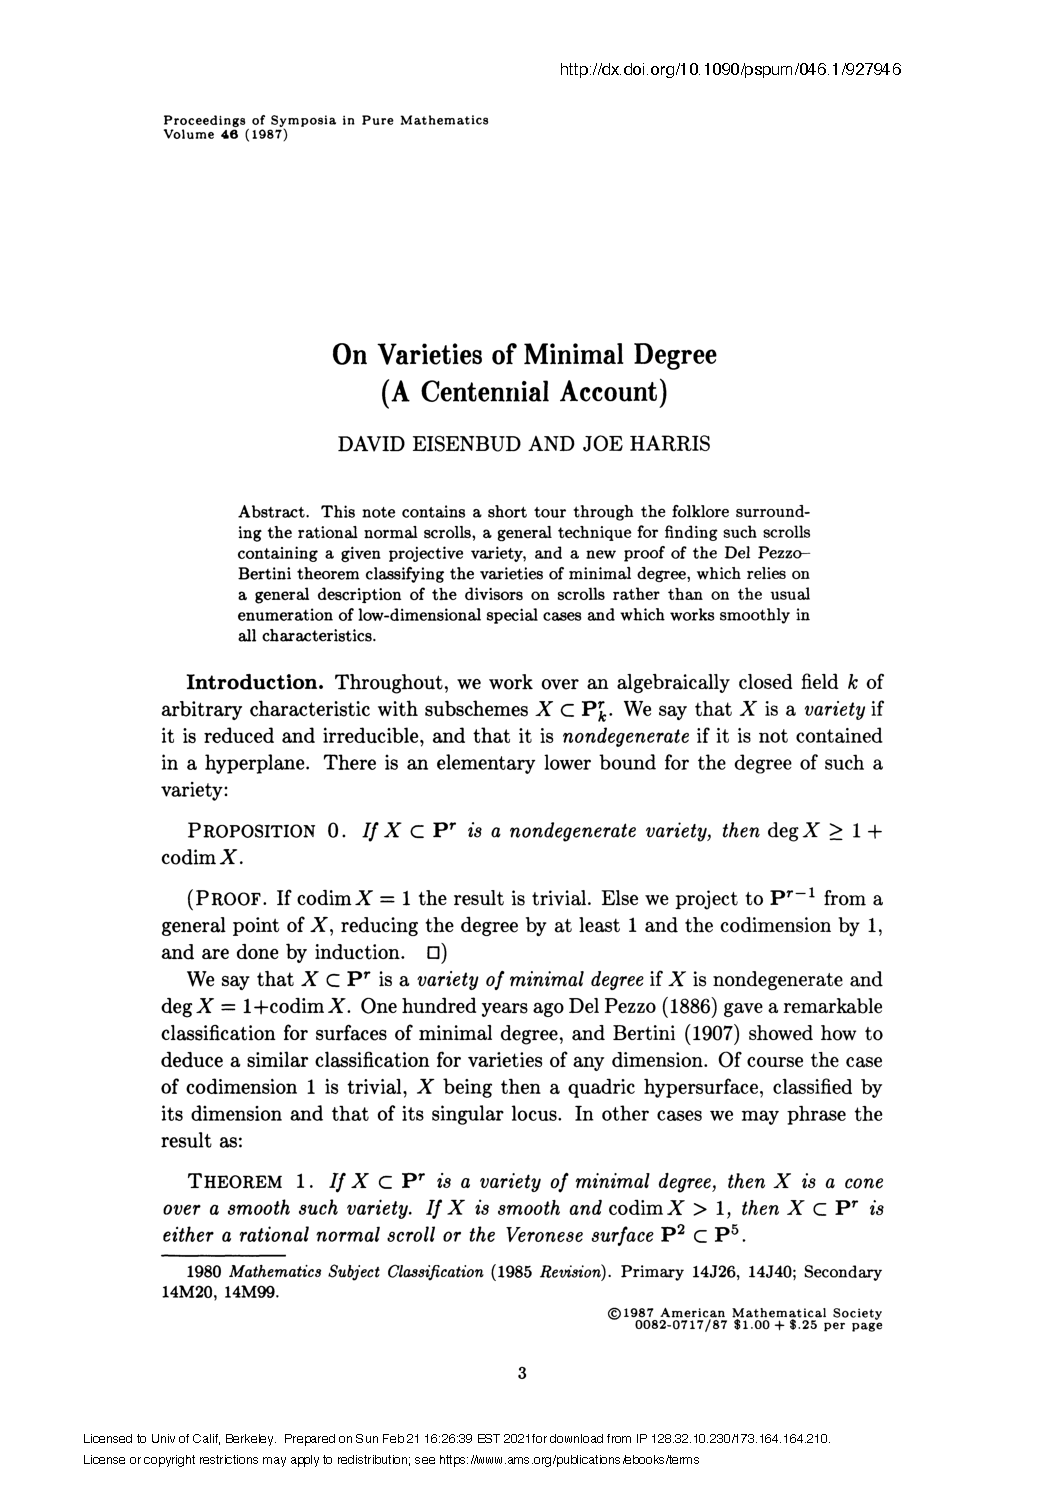
\includepdf[pages=1-11]{Centennial.pdf}


%footer for separate chapter files

\ifx\whole\undefined
%\makeatletter\def\@biblabel#1{#1]}\makeatother
\makeatletter \def\@biblabel#1{\ignorespaces} \makeatother
\bibliographystyle{msribib}
\bibliography{slag}

%%%% EXPLANATIONS:

% f and n
% some authors have all works collected at the end

\begingroup
%\catcode`\^\active
%if ^ is followed by 
% 1:  print f, gobble the following ^ and the next character
% 0:  print n, gobble the following ^
% any other letter: normal subscript
%\makeatletter
%\def^#1{\ifx1#1f\expandafter\@gobbletwo\else
%        \ifx0#1n\expandafter\expandafter\expandafter\@gobble
%        \else\sp{#1}\fi\fi}
%\makeatother
\let\moreadhoc\relax
\def\indexintro{%An author's cited works appear at the end of the
%author's entry; for conventions
%see the List of Citations on page~\pageref{loc}.  
%\smallbreak\noindent
%The letter `f' after a page number indicates a figure, `n' a footnote.
}
\printindex[gen]
\endgroup % end of \catcode
%requires makeindex
\end{document}
\else
\fi




%header and footer for separate chapter files

\ifx\whole\undefined
\documentclass[12pt, leqno]{book}
\usepackage{graphicx}
\input style-for-curves.sty
\usepackage{hyperref}
\usepackage{showkeys} %This shows the labels.
%\usepackage{SLAG,msribib,local}
%\usepackage{amsmath,amscd,amsthm,amssymb,amsxtra,latexsym,epsfig,epic,graphics}
%\usepackage[matrix,arrow,curve]{xy}
%\usepackage{graphicx}
%\usepackage{diagrams}
%
%%\usepackage{amsrefs}
%%%%%%%%%%%%%%%%%%%%%%%%%%%%%%%%%%%%%%%%%%
%%\textwidth16cm
%%\textheight20cm
%%\topmargin-2cm
%\oddsidemargin.8cm
%\evensidemargin1cm
%
%%%%%%Definitions
%\input preamble.tex
%\input style-for-curves.sty
%\def\TU{{\bf U}}
%\def\AA{{\mathbb A}}
%\def\BB{{\mathbb B}}
%\def\CC{{\mathbb C}}
%\def\QQ{{\mathbb Q}}
%\def\RR{{\mathbb R}}
%\def\facet{{\bf facet}}
%\def\image{{\rm image}}
%\def\cE{{\cal E}}
%\def\cF{{\cal F}}
%\def\cG{{\cal G}}
%\def\cH{{\cal H}}
%\def\cHom{{{\cal H}om}}
%\def\h{{\rm h}}
% \def\bs{{Boij-S\"oderberg{} }}
%
%\makeatletter
%\def\Ddots{\mathinner{\mkern1mu\raise\p@
%\vbox{\kern7\p@\hbox{.}}\mkern2mu
%\raise4\p@\hbox{.}\mkern2mu\raise7\p@\hbox{.}\mkern1mu}}
%\makeatother

%%
%\pagestyle{myheadings}

%\input style-for-curves.tex
%\documentclass{cambridge7A}
%\usepackage{hatcher_revised} 
%\usepackage{3264}
   
\errorcontextlines=1000
%\usepackage{makeidx}
\let\see\relax
\usepackage{makeidx}
\makeindex
% \index{word} in the doc; \index{variety!algebraic} gives variety, algebraic
% PUT a % after each \index{***}

\overfullrule=5pt
\catcode`\@\active
\def@{\mskip1.5mu} %produce a small space in math with an @

\title{Personalities of Curves}
\author{\copyright David Eisenbud and Joe Harris}
%%\includeonly{%
%0-intro,01-ChowRingDogma,02-FirstExamples,03-Grassmannians,04-GeneralGrassmannians
%,05-VectorBundlesAndChernClasses,06-LinesOnHypersurfaces,07-SingularElementsOfLinearSeries,
%08-ParameterSpaces,
%bib
%}

\date{\today}
%%\date{}
%\title{Curves}
%%{\normalsize ***Preliminary Version***}} 
%\author{David Eisenbud and Joe Harris }
%
%\begin{document}

\begin{document}
\maketitle

\pagenumbering{roman}
\setcounter{page}{5}
%\begin{5}
%\end{5}
\pagenumbering{arabic}
\tableofcontents
\fi


\chapter{Free resolutions and canonical curves}
\label{SyzygiesChapter}

\def\length{{\rm length}}

In Chapter~\ref{LinkageChapter} we related the resolutions of curves in $\PP^3$ to their Hartshorne-Rao modules. The
simplest case was that in which the Hartshorne-Rao module vanishes, that is, the case of arithmetically Cohen-Macaulay curves.
In this chapter we first quote a result that is a step toward understanding the structure of free resolutions, and use it to explain how the condition that a curve in $\PP^r$ is arithmetically Cohen-Macaulay manifests itself in the 
free resolution of the homogeneous ideal of the curve.  We will then introduce the Eagon-Northcott complexes, and explain their relation to the free resolutions of canonical curves. We close the chapter with an explanation of Green's conjecture, which proposes a way in which the intrinsic geometry
of a curve may be connected to the shape of its minimal free resolution of its ideal in the canonical embedding.

\begin{remark}
 There are two related contexts for the results of this section:  modules over a local ring, and graded modules over a polynomial ring whose variables have positive degree. These are parallel, essentially because Nakayama's lemma works in both cases. We will simply work with local rings or polynomial rings over a field with variables in degree 1 and leave the translations to the reader.\end{remark}

\section{Free resolutions}
A more complete presentation of the material in this section may be found in~\cite[Chapter 19]{Eisenbud1995}.


Let $M$ be a finitely generated graded module over $S := \CC[x_0, \dots x_r]$. A \emph{free resolution} of $M$ is an exact complex
of graded free modules, with maps of degree 0:
$$
(\FF, \phi):\quad 0\lTo M \lTo^\epsilon \bigoplus_jS(-j)^{\beta_{0,j}} \lTo\cdots
 \lTo^{\phi_t}\bigoplus_jS(-j)^{\beta_{t,j}}\lTo 0.
$$
Here $S(-j)$ denotes the graded free module of rank 1 with generator in degree $j$.
%$$
%\FF: \cdots \rTo F_s \rTo^{\phi_s} F_{s-1} \rTo^{\phi_{s-1}} \cdots \rTo F_1 \rTo^{\phi_1}  F_0 \rTo^\epsilon M \rTo 0.
%$$
(The map to $M$ is not considered part of the free resolution). The resolution is \emph{minimal} if a minimal set of generators of $F_i := \bigoplus_jS(-j)^{\beta_{t,j}}$ maps to a minimal set of generators of the kernel of the following map,
or equivalently (by Nakayama's lemma) the maps in $\FF\otimes_S \CC$ are all 0.

The first examples of a minimal free resolution are the Koszul complexes
(first defined, despite the name, in \cite{Cayley}, and repeated, as examples, 
in \cite{Hilbert1890}), which resolve $S/I$ when
 $I = (f_1,\dots, f_t)$
is a complete intersection, that is, $f_1,\dots, f_t$ is a regular sequence, with $\deg f_i = d_i$.  For $t = 2,3$, these look like

$$
%0\lTo S/I 
%\lTo^\epsilon 
S
\lTo^{ \begin{pmatrix}
f_1&f_2
\end{pmatrix}} 
S(-d_1)\oplus S(-d_2) 
\lTo^{\begin{pmatrix}
-f_2\\f_1
\end{pmatrix}}
 S(-d_1-d_2)\lTo 0,
$$
and
%\begin{tiny}
$$
%0\lTo S/I 
%\lTo^\epsilon 
S
\lTo^{
 \begin{pmatrix}
f_1&f_2&f_3
\end{pmatrix}} 
F_1\lTo^{
\begin{pmatrix}
 0&f_3&-f_2\\
 -f_3&0&f_1\\
 f_2&-f_1&0
\end{pmatrix}}
F_2
\lTo^{\begin{pmatrix}
f_1\\f_2\\f_3
\end{pmatrix}}
 F_3 \lTo 0,
$$
%\end{tiny}

where
$$
F_1 = \bigoplus_{j=1}^3S(-d_j),\
 F_2=
\bigoplus_{1\leq i <j\leq 3} S(-d_i-d_j) \text{ and }
F_3 = 
S(-d_1-d_2-d_3).
$$
%%

%and
%
%$$
%\begin{aligned}
%0\rTo S \rTo^{
%\begin{pmatrix}
%f_1\\f_2\\f_3
%\end{pmatrix}} S^3&\rTo{
%\begin{pmatrix}
% 0&f_3&-f_2\\
% -f_3&0&f_1\\
% f_2&-f_1&0
%\end{pmatrix}}
% S^3\rTo^{
% \begin{pmatrix}
%f_1&f_2&f_3
%\end{pmatrix}}
%S\rTo S/I \rTo 0
%\end{aligned}
%$$

Hilbert's Basis and Syzygy theorems together imply that every finitely generated $S$-module has a finite free resolution
of length no greater than the number of variables, $r+1$. (Fundamental
results of Auslander, Buchsbaum and Serre say that a local ring $R$ is \emph{regular}---that is, the Krull dimension of $R$ is equal to the minimal number
of generators of $\gm$---if and only if the minimal free resolution of the residue field is finite, in which case
the minimal free resolution of every module is finite.)

To construct this, suppose that a minimal homogeneous set of generators of $M$
contains $\beta_{0,j}$ generators of degree $j$ for each $j$; this defines a degree 0 map $\epsilon$
from 
$
\oplus_jS(-j)^{\beta_{0,j}}
$
onto $M$. We proceed similarly with the kernel of $\epsilon$, and continue to construct the whole resolution.
Hilbert's syzygy theorem \cite[Corollary 19.7]{Eisenbud1995} implies that the process ends after $t\leq r$ steps with a map $\phi_t$ whose
kernel is 0. 

The number $t$ is then the projective dimension of $M$. 
Equivalently, 
$$
\pd\ M = \max\{t \mid \Ext_S^t(M,k) \neq 0 \}.
$$
It follows from the Auslander-Buchsbaum
theorem~\cite[Theorem 19.9]{Eisenbud1995} that $t \geq \codim \ann_S(M)$, the codimension of the support of $M$.
Minimal free resolutions of a given module $M$ are all isomorphic.

\section{Classification of 1-generic \texorpdfstring{$2\times f$}{2 x f} matrices}\label{Kronecker}

We can use the uniqueness of minimal free resolutions to give a simple proof of Kronecker's classification of 1-generic $2\times f$
 matrices~\cite{Gantmacher}, which was announced in Chapter~\ref{ScrollsChapter}.
 
\begin{theorem}\label{matrix pencils}
 Every
 1-generic $2 \times f$ matrix of linear forms can be transformed by row and column operations and a linear change
 of variables to one of the type shown in
Corollary~\ref{equations of scrolls}, and thus the minors of any 1-generic matrix define a scroll. 
\end{theorem}


To prove this result we first reinterpret the 1-generic condition:
We have observed that an
$a\times b$ matrix of linear forms in $c$ variables is the same as a $\CC$-linear map of vector spaces
$A \otimes B \to C$, where $A, B$ and $C$ have dimensions $a,b$ and $c$ respectively. Such a map
can be viewed in several ways, for example as a map $C^{*} \otimes B\to A^{*}$---in other words, a $c\times b$ matrix in $a$ variables---or equivalently an $a$-dimensional family of $c\times b$ matrices (and similarly for other permutations of $A,B,C$). 
This bit of trivial formalism pays off in the following observation:

\begin{proposition}\label{reinterpretation of 1-generic}
An  $a\times b$ matrix of linear forms in $c$ variables $M$ corresponding to $A\otimes B \to C$ is 1-generic if and only if the $c \times b$ matrix $N$ of linear forms in $a$ variables corresponding to $C^{*}\otimes B \to A$ has constant rank $b$; that is, 
for point $x$ in $\PP^{a-1}$, the rank of $N$ evaluated at $x$ is $b$.
\end{proposition}

\begin{proof}
The $b$ columns of $N$ correspond to the $b$ columns of $M$, while the rows of $N$ are indexed
by the $c$ variables in $M$ and the variables in $N$ are indexed by the $a$ rows of $M$. Thus the
evaluation of $N$ at a point $x$ corresponds to a generalized row of $M$; and the image of $N(x)$
is the span of the variables in that generalized row. The matrix $M$ is 1-generic if the dimension
of that span is $b$ for every generalized row.
\end{proof}

Thus the classification of 1-generic $2\times f$ matrices of linear forms in $r+1$ variables of Theorem~\ref{matrix pencils} is equivalent to the classification
of \emph{matrix pencils} of constant maximal rank---that is $f \times (r+1)$ matrices of linear forms over $\PP^{1}$ with constant rank $r$.
Such ``matrix pencils'' were first classified by Kronecker; see 
\cite[Vol. II, Chapter 12]{Gantmacher} for an exposition, and ~\cite{Eisenbud-Harris-Centennial} for a geometric approach.
We will give a still simpler proof:

\begin{proof}[Proof of Theorem~\ref{matrix pencils}]
Let $M$ be a 1-generic $2\times b$ matrix in $r+1$ variables. We may assume that the span of the entries
is equal to the vector space of linear forms in $\PP^{r}$. The associated 
$(r+1)\times b$ matrix
$$
N: \sO_{\PP^{1}}(-1)^{b} \to \sO_{\PP^{1}}^{r+1}
$$
 of linear forms over $\PP^{1}$ has constant rank $b$.
For every point $x\in \PP^{1}$ the scalar matrix $N(x)$ is a split inclusion, and thus
$\coker N$ is a vector bundle, necessarily isomorphic to $\sum_{i =1}^{d}\sO_{\PP^{1}}(a_{i})$ for some
integers $a_{i}\geq 0$. 

Regarded as a matrix over $\CC[s,t]$ it follows that the exact sequence
$$
0\to \sO_{\PP^{1}}(-1)^{b} \rTo^{N} \sO_{\PP^{1}}^{r+1}  \rTo \bigoplus_{i = 1}^{d}\bigl( \oplus_{j=0}^{\infty}H^{0}(\sO_{\PP^{1}}(j-a_{i}))\bigr)\rTo 0
$$
is a minimal free resolution. It follows that the map $N$ is the direct sum of the minimal free resolutions over $\CC[s,t]$
of the modules 
$$
\bigoplus_{j=0}^{\infty}H^{0}(\sO_{\PP^{1}}(j-a_{i})) = (s,t)^{a_{i}}.
$$
As we will explain in Example~\ref{res of max ideal power}, the minimal presentation of $(s,t)^{a_{i}}$ is the $(a_{i}+1)\times a_{i}$ matrix
$$
\begin{pmatrix}
s&0&0&\dots&0\\
-t&s&0&\dots&0\\
0&-t&s&\dots&0\\
0&0&-t&\dots&0\\
\vdots&&\cdots&&\vdots\\
0&&\dots&\ddots&s\\
0&&\dots&\dots&-t\\
\end{pmatrix}
$$
The direct sum decomposition of $N$ corresponds to a block decomposition of $M$,
and thus after a change of bases and variables the matrix $N$ is transformed into the direct sum of these matrices.
Translating this form back to a $2\times (r+d-1)$ matrix $M$, we have transformed $M$ into a matrix of 
the desired form.
\end{proof}

\subsection{How to look at a resolution}
As is apparent even in the example $t=3$ above, free resolutions can be bulky to describe; the 
\emph{Betti table} is a compact representation of the numerical information in the resolution.
Suppose that 
$F$ is a minimal free resolution of a module $M$ as illustrated in the beginning of the previous section. Since we choose a minimal set of generators at each stage, the matrices of the $\phi_i$ have entries in the maximal
ideal $(x_0,\dots x_r)$, and thus each $\beta_{i+1, j}$ must be strictly greater than some $\beta_{i,j}$. For this reason it
is convenient to tabulate the numbers so that $\beta_{i,j}$ is in the $i$-th column and $(j-i)$-th row:
$$
\scriptsize{
\begin{matrix} 
j\backslash i&\vline&0   &  1    & \cdots & n    \cr\hline
\vdots&\vline&\vdots&\vdots & \cdots    &\vdots     \cr 
       0&\vline&\beta_{0,0}&\beta_{1,1}&\cdots&\beta_{n,n}\cr
       1&\vline&\beta_{0,1}&\beta_{1,2}&\cdots&\beta_{n,n+1}\cr
\vdots&\vline&\vdots&\vdots & \cdots    &\vdots     \cr 
\end{matrix}.
}
$$         

\begin{example}
 The Koszul complex that resolves the homogeneous coordinate ring $S/(Q, F_1, F_2)$ of the complete intersection of  2 quadrics and a cubic in $\PP^3$ has the form
$$
S \lTo S(-2)\oplus S(-3)^2 \lTo S(-5)^2\oplus S(-6) \lTo S(-8) \lTo 0,
$$
which has Betti table:

\centerline{\scriptsize
\begin{tabular}{r|ccccc} 
$j\backslash i$&0&1&2&3\\ 
\hline 
0&1&$-$&$-$&$-$\\ 
1&$-$&1&$-$&$-$\\
2&$-$&2&$-$&$-$\\
3&$-$&$-$&$2$&$-$\\
4&$-$&$-$&$1$&$-$\\
5&$-$&$-$&$-$&$1$\\
\end{tabular}.}
\end{example}

 To simplify our language, we will speak of the \emph{Betti table of a scheme $X$} rather than the ``Betti table of the minimal free resolution of the ideal of $X$".

\subsection{When is a finite free complex a resolution?}
How does a free resolution over $S := \CC[x_0, \dots x_r]$ ``know'' to end no later than the $(r+1)$-st step? 
The following result describes a sense in which the maps in the resolution change as the resolution continues.
The result is proven in~\cite[Theorem 20.9]{Eisenbud1995}. 

A central role in the theorem is played by the ideals of minors of the differentials in the complex: If $\phi: F\to G$ is a map of finitely generated free $R$-modules with cokernel $M$, then
$I_t(\phi)$ denotes the ideal generated by all the $t\times t$ minors (=subdeterminants) of a matrix representing $\phi$; this is independent of the choice of bases used to represent $\phi$ as a matrix.
The ideal $I_{\rank G -j}(\phi)$ depends only on $M$; it called the $j$-th Fitting ideal of $\coker \phi$  and 
usually written $\Fitt_{j}(M)$. Some basic properties of these ideals are
given in Exercise~\ref{Fitt}, where the reader may show that the annihilator of $M$ has the
same radical as $\Fitt_{0}(M)$. Actually more is true: 

\begin{fact}
If $F\to G \to M \to 0$ is an exact sequence of finitely generated $R$-modules, then 
$$
\ann_{R}(\coker \phi)^{\rank G}\subset Fitt_{0}(\phi) \subset \ann_{R}(\coker \phi).
$$
For this and other such inequalities, see~\cite{MR476736}.
\end{fact}

The \emph{rank} of $\phi: F\to G$ is the largest size of a nonvanishing minor of a matrix for $\phi$,
or equivalently the largest $k$ such that the exterior power $\wedge^{k}\phi : \wedge^{k}F \to \wedge^{k}G$
is nonzero. If $r:= \rank \phi = \rank G$, then the ideal $I(\phi): = I_{\rank \phi}(\phi)$ plays a special role: the cokernel of $\phi$
is projective (= locally free) if and only if $I(\phi) = R$. If $I(\phi)$ contains a non-zerodivisor, then
the construction localizes, and we see that $I(\phi)$ defines the locus  $P\in \Spec R$ where $(\coker \phi)_{P}$
is not free. 


Recall that the grade of an ideal is the length of a maximal regular sequence
contained in it, or $\infty$ if $I=R$. If $R$ is a Cohen-Macaulay ring---for example $\CC[x_{0},\dots, x_{r}]$---then the grade of any proper ideal is equal to its codimension, so grade becomes a geometric notion.
Readers less familiar with commutative algebra will lose little if they stick with the case when $R$ is
regular, or even the case when $R$ is $\CC[x_{0},\dots, x_{r}]$. This suffices, for example for the applications
of the Eagon-Northcott complex described below.


\begin{theorem}\label{WMACE}
 Let $R$ be a Noetherian ring and let
 $$ 
\FF:  F_0\lTo^{\phi_1}F_1 \lTo \cdots \lTo F_{n-1}\lTo^{\phi_n} F_n\lTo 0
 $$
be a finite complex of free $S$-modules. Set $r_i := \rank \phi_i$. 
The complex $\FF$ is \emph{acyclic} (that is, $H_i(\FF) = 0$ for all $i>0$) if and only if
\begin{enumerate}
 \item $\rank F_i = r_i+r_{i+1}$; and
 \item $\grade I_{r_{i}}(\phi_i) \geq i$.
\end{enumerate}
for all $i$.
\qed
\end{theorem}

In particular, if $R$ is Noetherian, then a map of finitely generated free modules  $G\lTo^{\phi}F$ is injective 
if and only if $I_{\rank F}(\phi)$ contains a non-zerodivisor.

A familiar case occurs when  $r=1$ and $R$ is a domain. In this case the theorem says that a map $F_1\to F_0$ is a monomorphism iff it becomes a monomorphism after tensoring with the field of rational functions $K$, which follows from the flatness of
localization and the fact that $F_1$ is torsion-free, so that
$F_1 \subset F_1 \otimes K$. 

To see the relevance of the second hypothesis to the conclusion, suppose for a moment that $R$ is
a regular local ring of dimension $r$, and suppose that the complex $\FF$ is acyclic. The hypothesis $\grade I(\phi_{d+1}) \geq d+1$ can only be satisfied if $I(\phi_{d+1}) = R$ (so that its grade is $\infty$ by convention). This  is equivalent to the cokernel of $\phi_{d+1}$ being free. Thus the theorem ``explains'' why a minimal free resolution
has length $\leq r+1$.

\section{Depth and the Cohen-Macaulay property}

If $M$ is a graded  $\CC[x_0, \dots x_r]$-module then an \emph{$M$-regular sequence} is a sequence of homogeneous polynomials
$f_1,\dots,f_m \in (x_0,\dots, x_r)$ such that $f_1$ is a non-zerodivisor on $M$, $f_2$ is a non-zerodivisor on $M/(f_1M)$, and so on. 
The maximal length of such a sequence is called the \emph{depth} of $M$, or more properly the depth of $(x_0,\dots, x_r)$ on $M$.
The length of any all maximal $M$-regular sequences are the same, as one shows by proving

\begin{theorem} (Auslander-Buchsbaum)\label{Auslander-Buchsbaum}
If $M$ is a finitely generated $S := \CC[x_0, \dots x_r]$-module, then the length of every $M$-regular sequence is $m = r+1 - \pd\  M$,
and $m$ is the smallest integer $m$ such that $\Ext_S^m(S/(x_0, \dots x_r), M) \neq 0$.
\end{theorem}
 
 The depth of a module $M$ is bounded above by $\dim M$, the Krull dimension. The reason is that if the dimension of $M$
 is $d$, and $f_1 \in (x_0, \dots x_r) $ is a non-zerodivisor on $M$, then $\dim M/(f_1)M= \dim M-1$. Thus by induction, if
  $f_1,\dots, f_d$ is $M$-regular then $M/(f_1, \dots, f_d)M$ has dimension 0, which is equivalent to its being Artinian. Thus any 
$ f_{d+1} \in(x_0, \dots x_r) $ acts as a nilpotent endomorphism of $M/(f_1, \dots, f_d)M$.

It follows from these facts that the depth of an $S$-module $M$ is equal to the dimension of $M$ if and only if the projective dimension
of $M$ is equal to the codimension of $M$; in this case we say that $M$ is a
\emph{Cohen-Macaulay module}. 

As we showed in Chapter~\ref{linkageChapter}, a curve $C\subset \PP^3$ is linked to a complete intersection
if and only if  $H^1_*(\sI_C) := \oplus_{m\in \ZZ} H^1(\sI_C(m)) = 0$, in which case $C$ is said to be is arithmetically Cohen-Macaulay.
From the Auslander-Buchsbaum theorem and Theorem~\ref{ACM basics} we see that $C$ is arithmetically Cohen-Macaulay if
and only if the homogeneous coordinate ring $R_C$ is Cohen-Macaulay, and this is true
if and only if $\pd\  R_C = \codim C$.


\subsection{The Gorenstein property} 
Another important homological condition is the condition that $\omega_X$ is an invertible sheaf; when this holds, we say that $X$ is \emph{quasi-Gorenstein}. When, in addition, $X$ is Cohen-Macaulay we say that $X$ is \emph{Gorenstein}. Any scheme that is locally a complete intersection, such as any smooth scheme, is Gorenstein. Since the restriction
of $\sO_{\PP^r}(1)$ to a subvariety is always invertible, saying that a scheme $X$ is canonically embedded implies that
$X$ is at least quasi-Gorenstein. As with the Cohen-Macaulay property, the Gorenstein property is interpreted locally
on a scheme. We say that a projective scheme $X$ is \emph{arithmetically Gorenstein}
if its homogeneous coordinate ring is Gorenstein, and it follows that $\omega_{S/I} \cong S/I(a)$ for some integer $a = a(X)$.

In Chapter~\ref{LinkageChapter},  we expressed $\omega_X$
for a subscheme $X\subset Y$ of a scheme $Y$ as
 $\Ext^{\codim X}_{\sO_Y}(\sO_X, \omega_Y)$. Slightly extending this idea, if $C\subset \PP^r$ is a curve
with homogeneous coordinate ring $R_{C}$,
 we define $\omega_{R_C}$ to be $\Ext^{r-1}_S(R_C, S(-r-1))$, where $S$ is the homogeneous coordinate ring of $\PP^r$.
Since $\omega_{\PP^r} = \sO_{\PP^r}(-r-1)$, the sheafification of this module is  $\omega_C$.

If $C$ is arithmetically Cohen-Macaulay, so that
$\pd (C) = \codim(C) = r-1$,  then 
computing $\Ext^{r-1}_S(R_C, S(-r-1))$ from the minimal free resolution 
$$
(\FF, \phi):\quad 0\lTo R_C \lTo S\lTo^{\phi_1} F_1 \lTo \cdots \lTo F_{r-2} \lTo^{\phi_{r-1}} F_r\lTo 0
$$
we see that $\omega_{R_C} = \coker \phi_{r-1}^*$. Theorem~\ref{WMACE} implies that the complex $(\FF^*, \phi^*)$ which is the dual
of the  resolution $(\FF, \phi)$ is again acyclic, so it is the minimal free resolution of $\omega_{R_C}$. Thus 
$\omega_{R_C}$ is a Cohen-Macaulay module. Just as the Cohen-Macaulay property of
$R_C$ implies that $R_C = H^0_*(\sO_C)$, it follows that $\omega_{R_C} = H^0_*(\omega_C)$.

If, in addition, $C$ is a canonical curve, so that $\omega_C = \sO_C(1)$, then we derive:
$$
\omega_{R_C} = \coker(\phi_{r-2}^*)(-r-1) = R_C(1)
$$
so $\coker \phi_{r-2}^* = R_C(r)$. Thus $(\FF^*(-r), \phi^*)$ is a minimal free resolution of $R_C$, and is therefore isomorphic to
$(\FF^*, \phi^*)$; that is, $(\FF^*, \phi^*)$ is self-dual.
 We have seen an example already
in the Koszul complex (a complete intersection is arithmetically Gorenstein).

Taking into account that in a resolution $(\FF, \phi)$ each summand $S(-j)$ of $F_{i+1}$ can only
map to summands $S(-l)$ of $F_i$ with $\ell < j$, and similarly for the dual, we see that the 
Betti table of the minimal free resolution of a canonical curve of genus $g$ must have the form:


% \centerline{\scriptsize
%\begin{tabular}{r|cccccc} 
%$j\backslash i$&0&1&2&$\cdots$&$r-2$&$r-1$\\ 
%\hline 
%0&1&$-$&$-$&$\cdots$&$-$&$-$\\ 
%1&$-$&$\binom{g-2}{2}$&$?$&$\cdots$&$?$&$-$\\
%2&$-$&?&$?$&$\cdots$&$\binom{g-2}{2}$&$-$\\
%3&$-$&$-$&$-$&$\cdots$&$-$&$1$\\
%\end{tabular}.}
%
%\centerline{\scriptsize
%\begin{tabular}{r|cccccc} 
%$j\backslash i$&0&1&2&$\cdots$&$r-2$&$r-1$\\ 
%\hline 
%0&1&$-$&$-$&$\cdots$&$-$&$-$\\ 
%1&$-$&$\binom{g-2}{2}$&$b_2$&$\cdots$&$b_{r-2}$&$-$\\
%2&$-$&$b_{r-2}$&$b_{r-3}$&$\cdots$&$\binom{g-2}{2}$&$-$\\
%3&$-$&$-$&$-$&$\cdots$&$-$&$1$\\
%\end{tabular}.}

\centerline{\scriptsize
\begin{tabular}{r|cccccc} 
$j\backslash i$&0&1&2&$\cdots$&$g-3$&$g-2$\\ 
\hline 
0&1&$-$&$-$&$\cdots$&$-$&$-$\\ 
1&$-$&$b_1$&$b_2$&$\cdots$&$b_{g-3}$&$-$\\
2&$-$&$b_{g-3}$&$b_{g-4}$&$\cdots$&$b_1$&$-$\\
3&$-$&$-$&$-$&$\cdots$&$-$&$1$\\
\end{tabular}.}
\noindent where  $-$ represents 0.  It turns out that the $b_i$ depend on the particular canonical curve,
but since the Hilbert function of the curve is the alternating sum of the Hilbert functions in the resolution,
the differences $b_i- b_{g-i-1}$ are independent of the curve.

To go further, we can make use of the invertible sheaves $\sL$ on $C$ with $h^0(\sL)=2$ and $h^1(\sL)\geq 2$. 
The existence of such a series guarantees that the ideal of $C$ contains the ideal of $2\times 2$ minors of the $2\times h^1(\sL)$
matrix
corresponding to the multiplication map 
$H^0(\sL) \otimes H^0(\sL^{-1}\otimes \omega_C) \to H^0(\omega_C) = H^0(\sO_C(1))$
as in Chapter~\ref{ScrollsChapter}.
The mechanism is a resolution of
the ideal generated by the minors of this matrix.
 
\section{The Eagon-Northcott complex}\label{EN section}

The Eagon-Northcott complex $EN(\phi)$~\cite{MR0142592} associated with a matrix, or a map of free modules $\phi: F\to G$,
is a generalization of the Koszul complex, which is the case $\rank G = 1$. Like the Koszul complex,
it is tautological: its existence depends only on the properties of commutative rings; and like the Koszul complex it is exact or not depending on a property of the matrix $\phi$ related to regular sequences. It is part of a family of complexes described in
\cite[Appendix A2]{Eisenbud1995}, and, from a more conceptual and general point of view, in \cite{Weyman-book}. 

We
are interested in $EN(\phi)$ because its shape
influences the shape of the free resolutions of canonical curves in an interesting way, 
leading to Green's conjecture. This conjecture, one of the central open problems in the theory of algebraic curves, is described in the last
section of this chapter. We will also use the the Eagon-Northcott complex, in a special case, to give a proof of the classification of matrix pencils and an analysis of the ideals of ACM curves in $\PP^{3}$.

To prepare for the description of the Eagon-Northcott complex we revisit the Koszul complex, which is equal
to the Eagon-Northcott complex in the case $\rank G = 1$, and then consider the case $\rank F = \rank G + 1$.

\subsubsection{$\mathbf {\bf rank\ }  \mathbf{G = 1}$}

In this subsection we let $\phi:F = R^{f}\to R$ be a homomorphism from a free module to a ring $R$, and we
we will analyze the Koszul complex $K(\phi)$. 

We may write
$K(\phi) = EN(\phi)$ in the form
$$
S \lTo^{\delta_{1}} F \lTo^{\delta_{2}} \wedge^{2}F \lTo^{\delta_{3}} \cdots \lTo^{\delta_{f}} \wedge^{f}F \lTo 0
$$
where $\delta_{1} = \phi$.

To define the complex, we must construct the differentials $\delta_{i}$ and prove that
$\delta_{i}\delta_{i+1} = 0$. Since the modules are free, it suffices to do this for the 
dual maps 
$$
\partial_{i}: \wedge^{i}F^{*} \to \wedge^{i+1}F^{*},
$$
and it turns out that this is in a sense even more natural. 

It is convenient to think of $R$ as an $S := \ZZ[x_{1},\dots, x_{f}]$-algebra by the map sending 
$x_{i}$ to $\phi_{i}$; we  define the Koszul complex of $\phi$ over $R$ by tensoring
the Koszul complex of $(x_{1}, \dots, x_{f})$ with $R$.

Thus for the definition we take the map $\phi$ to be 
$$
\phi: S^{f}\rTo^{
\begin{pmatrix}
x_{1} &\dots & x_{f}
\end{pmatrix}
} S.
$$

First of all, the map $\partial_{i}$ (like the map $\delta_{i}$) is \emph{linear}: the image of a basis vector of $\wedge^{i}F^{*} $ is a sum of variables times basis vectors
of $\wedge^{i+1}F^{*}$. We may write $S$ as $\Sym(V)$, where $V$ is the free $\ZZ$-module generated by $x_{1}, \dots, x_{f}$, and we may think of $F$ as the module $V\otimes S$ with the map
$\phi$ sending $V\otimes 1\subset F$ by the identity to $V = S_{1}\subset S$---the ``tautological map''. 
Let $t\in V\otimes V^{*}\subset S\otimes \wedge V^{*}$ be the ``trace element'' represented in terms of any basis $\{x_{i}\}$ of $V$
and dual basis $\{\hat e_{i}\}$ of $V^{*}$ as $t = \sum x_{i}\otimes \hat e_{i}$. Because $\wedge V^{*}$ is 
an anti-commutative algebra, we have $t^{2} = 0$.

We define the map 
$$
\partial_{i}: S\otimes_{\CC} \wedge^{i}V^{*} = \wedge^{i}F^{*}  \to \wedge^{i+1}F^{*} = S\otimes_{\CC} \wedge^{i+1}V^{*}
$$
to be multiplcation by $t$, and thus $\partial_{i+1}\partial_{i}$ is multiplication by $t^{2} = 0$.

Having defined the complex $K(\phi) = EN(\phi)$ in the case $\rank G = 1$, we next ask what conditions on $\phi$
make it acyclic (that is, a free resolution of $\coker (\delta_{1})$). 

\begin{theorem}\label{rankG1}
 Suppose that $R$ is a ring and $\phi: F\to R$ is a map from a free $R$-module of rank $f$.
 The complex $K(\phi)$ is acyclic if and only if the ideal $I := I_{1}(\phi)$ has grade $\geq f$.
 \end{theorem}

\begin{proof}
Theorem~\ref{WMACE} immediately implies that if $K(\phi)$ is acyclic then
$\rank \delta_{f} = 1$ and $\grade I(\delta_{f}) \geq f$. Since $I(\delta_{f}) = I$, this proves one implication.

Now assume that $\grade I \geq f$. We first prove that 
$K(\phi)$ is split exact when $I = R$; that is, $\wedge^{i}F = \ker \delta_{i} \oplus \image\ \delta_{i}$ for every $i$, or equivalently
$\wedge^{i}F^{*} = \image\ \partial_{i}\oplus\coker \partial_{i}$ for every $i$. The condition $I=R$ implies that $\delta_{1}$ is s split surjection, 
or equivalently that 
 $\partial_{1}$ is a split injection. In this case we may write $F^{*} = R\oplus F'^{*}$ in such a way that $\partial_{1}$ is the injection into the first summand, and we may
choose a basis $\{\hat e_{i}\}$ of $F^{*}$ so that the last $f-1$ basis elements are a basis for $F'^{*}$. 
Specializing the sequence $x_{1},x_{2}, \dots, x_{f}$ to the sequence $1, 0,\dots, 0$, the differential of $K(\phi)^{*}$
becomes the multiplication by  $1\otimes e_{1}$.

The module
$\wedge^{i}F^{*}$  decomposes as 
$$
\wedge^{i}F^{*} = \bigl(Re_{1}\otimes_{R} \wedge^{i-1}F^{*} \bigr) \oplus \wedge^{i}F'^{*}.
$$
Because $e_{1}\wedge e_{1} = 0$ the differential $\partial_{i}$ has the form
$$
\begin{diagram}
&&Re_{1}\otimes \wedge^{i-2}F'^{*} &\rTo^{0}&  Re_{1}\otimes \wedge^{i-1}F'^{*}\\
\wedge^{i-1}F^{*}&=& \bigoplus&\ruTo^{\cong}&\bigoplus&=&\wedge^{i}F^{*}\\
 &&\wedge^{i-1}F'^{*}&\rTo^{0}& \wedge^{i}F'^{*}
\end{diagram}.
$$
Thus we see that $K(\phi)$ is split exact when $\phi$ is a split surjection.

We now assume only that $\grade I\geq f$. From what we just proved we see that if we localize
$R$ by inverting any element of $I$ the complex $K(\phi)$ becomes split exact. Since $\grade f\geq 1$,
we can find such  a non-zerodivisor in $I$, and inverting it does not change the ranks of the 
maps $\phi_{i}$. Because ranks of free modules are additive in direct sums, it is obvious that
in the split exact case the condition on the ranks of the $\phi_{i}$ is satisfied; more precisely,
$\rank(\delta_{i}) = \binom{i-1}{f-1}$. We also see that after inverting
a non-zerodivisor in $I(\delta_{1})$ we have $I(\delta_{i}) = R$; equivalently, 
$$
I  \subset \sqrt {I(\delta_{i})}.
$$
(In fact $I(\delta_{i}) = I^{\binom{i-1}{f-1}}$, though this requires a separate argument.) Thus if $\grade I = f$ then  $\grade I(\delta_{i}) \geq i$ for all $i$, so $K(\phi)$ is acyclic.
\end{proof}


\subsubsection{ $\mathbf{{\bf rank\ } F = {\bf rank\ }G + 1}$}

We set $g=\rank G$ and $f = \rank F = g+1$. In this case the Eagon-Northcott complex has the form:
$$
EN(\phi):\quad 0\rTo G^{*}\otimes \wedge^{f}F \rTo^{\delta_{2}} \wedge^{f-1}F \rTo^{\delta_{1}} \wedge^gG.
$$
Here $\delta_{1} = \wedge^{g}\phi$, so that the entries of a matrix for $\delta_{1}$ are the $g\times g$ minors of 
$\phi$.

We choose an identification $\wedge^{f}F = S$, called an \emph{orientation} of $F$, and get a perfect pairing 
$$
\wedge^{g}F \times F \to \wedge^{f}F = S
$$
so that we may identify
 $\wedge^{g}F$ with $F^{*}$. With this identification, we define $\delta_{2}$ as
 $$
\delta_{2}:  G^{*}\rTo^{\phi^{*}}  F^{*} = \wedge^{g}F.
 $$
We also choose an orientation $\wedge^{g}G = S$, in terms of which the image of $\delta_{1}$ is
 the ideal generated by the $(f-1)\times (f-1)$  minors of $\phi$.
 
We first claim that $EN(\phi)$ is a complex; that is,  $\delta_{1}\delta_{2} = 0$.  As with the Koszul complex,
it is convenient to dualize and consider the maps 
$$
EN(\phi)^{*}:\quad 0\rTo \wedge^{g} G \to \wedge^{g}F^{*} = F \rTo^{\phi} G
$$
The fact that this composition is 0 is often taught as Cramer's rule for solving a system of
homogeneous equations represented by a $g\times (g+1)$ matrix of rank $g$.
The solutions---that is, the elements of $\ker \phi$---are multiples of the column
$\Delta_{1}, \dots, \Delta_{g}$ where the $\Delta_{j}$ is $-1^{j}$ times the determinant
of the matrix obtained from $\phi$ by leaving out the $j$-th column. This works
because the composition of the two maps is a column matrix whose $i$-th entry is the
expansion of the $(g+1)\times (g+1)$ determinant of the matrix obtained from $\phi$ by
repeating the $i$-th row.

\begin{theorem}\label{EN grade 2}
 Suppose that $R$ is a ring and $\phi: F\to G$ is a map of  free $R$-modules, 
 where $G$ has rank $g$ and $F$ has rank $f = g+1$.
 The complex $EN(\phi)$ is acyclic if and only if the ideal $I := I_{g}(\phi)$ has grade $\geq 2$.
 \end{theorem}

%\begin{theorem}
%If $\phi$ is a $g\times (g+1)$ homogeneous matrix of forms of positive degree in $S$ then the Eagon-Northcott
%complex $EN(\phi)$ is acyclic if and only if $\grade I_{g}(\phi) \geq 2$.
%\end{theorem}

\begin{example}
We have seen that the ideal of the twisted cubic is generated by the $2\times 2$ minors of the matrix
$$
\phi :=  
\begin{pmatrix}
 x_{0}&x_{1}&x_{2}\\
 x_{1}&x_{2}&x_{3}
\end{pmatrix}
$$
and it follows that the free resolution of its homogeneous coordinate ring is the Eagon-Northcott complex
$$
0\rTo S^{2}(-3) 
\rTo^{\begin{pmatrix}
 x_{0}&x_{1}\\
  x_{1}&x_{2}\\
x_{2}&x_{3}
\end{pmatrix}
}
S^{3}(-2)
\rTo^{\wedge^{2}\phi}
S
$$
\end{example}

\begin{example}\label{res of max ideal power}
In Section~\ref{Kronecker} we asserted that  the $(a+1)\times a$  matrix
$$
\phi_{a} :=\begin{pmatrix}
s&0&0&\dots&0\\
-t&s&0&\dots&0\\
0&-t&s&\dots&0\\
0&0&-t&\dots&0\\
\vdots&&\cdots&&\vdots\\
0&&\dots&\ddots&s\\
0&&\dots&\dots&-t\\
\end{pmatrix}
$$
is the minimal presentation of the ideal $(s^{a},s^{a-1}t, \dots, t^{a}) \subset R:=\CC[s,t]$. It is not hard to check this
directly, but in any case it's easy to see that its $a\times a$ minors of $\phi_{a}$ generate this ideal, which has grade 2, so the Eagon-Northcott resolution $EN(\phi)$
has the form
$$
R\lTo^{\wedge^{a}\phi_{a}} R^{a+1} \lTo^{ \phi_{a}} R^{a} \lTo 0
$$
verifying the assertion.
\end{example}

\begin{proof}
Once having shown that $EN(\phi)$ is a complex, as we did above,  the proof of the equivalence in the theorem follows the same pattern as the
proof given above for the Koszul complex.

If $EN(\phi)$ is acyclic, then by Theorem~\ref{WMACE} the $g\times g$ minors of $\phi = \delta_{2}$ must
have grade $\geq 2$.
For the converse, suppose first that
$I_{g}(\phi)$ is the
unit ideal. We may split  $F$ as  $S\oplus G$ with $\Delta_{1} = 1$ and $\Delta_{j} = 0$
for $j>1$, and then $EN(\phi)^{*}$ has the form:
$$
\begin{diagram}
&&0&\rTo&  G&\rTo^{0}&S\\
0&\rTo& \bigoplus&\ruTo^{\cong}&\bigoplus&\ruTo^{\cong}&\bigoplus\\
 &&G&\rTo^{0}&S&\rTo&0
\end{diagram}.
$$
Thus we see that $EN(\phi)$ is split exact in this case.

We now apply Theorem~\ref{WMACE}: From what we just proved we see that if we localize
$S$ by inverting any element of $I$ then the complex $EN(\phi)$ becomes split exact,
and therefore, before localizing,
$\rank(\delta_{1}) = 1$ and $\rank \delta_{2} = g$ . In this
case it follows from the definition that $I_{1}(\delta_{1}) = I_{g}(\phi) = I_{g}(\delta_{2})$
so if $I_{g}(\phi)$ has grade 2 then both conditions of Theorem~\ref{WMACE} are
satisfied.
\end{proof}

\subsection{The Hilbert-Burch theorem}

In a regular local ring any ideal of codimension 1 is principal (divisors are all Cartier). What about
ideals of codimension 2? The answer is the content of the \emph{Hilbert-Burch} theorem, proven
in 1890 by David Hilbert in the case of homogeneous ideals in $\CC[x_{0},x_{1}]$ and in general by
Lindsay Burch~\cite{MR212008}. We can deduce it as an application of the Eagon-Northcott complex
in the case $f =g+1$:

\begin{corollary}[Hilbert-Burch theorem]\label{Hilbert-Burch}
Suppose that $R$ is a local ring. Any ideal $I\subset R$ of projective dimension 1 and grade 2 has the form
$aI'$ where $I'$ is an ideal of grade 2 generated by the $g\times g$ minors
of a $g \times (g+1)$ matrix and $a$ is a non-zerodivisor of $R$; and conversely any ideal of this form
has projective dimension 1. 

In particular, if $C\subset \PP^{3}$ is an ACM curve whose homogeneous ideal $I$ is generated by
$f$ elements, then $I$ is minimally generated by the $(f-1)\times (f-1)$ minors of the syzygy matrix of $I$.
\end{corollary}

\begin{proof}
If $C\subset \PP^{3}$ is ACM, then the projective dimension of the homogeneous coordinate ring $R_{C}$
is 2  by the Auslander-Buchsbaum theorem, and thus the ideal of $C$ has projective dimension 1.

Now suppose that $I\subset R$ is an ideal of projective dimension 1 in any local ring, and suppose
that $I$ is generated by $f$ elements, so that we have a surjection $F:= R^{f} \to I$.  The module $R/I$
has free resolution of the form
$$
\FF: R\lTo^{\alpha} R^{f}\lTo^{\phi} G\lTo 0
$$
where $I = I_{1}(\alpha)$, so by Theorem~\ref{WMACE} the free module $G$ has rank $g = f-1$, the $g\times g$
minors of $\phi$ generate an ideal $I'$ of grade $\geq 2$, and the ideal $I$ has grade $\geq 1$. Theorem~\ref{WMACE} implies
that both the Eagon-Northcott complex $EN(\phi)$
and its dual are acyclic. 

The dual of the complex $\FF$ will not be acyclic unless $\grade I = 2$, but there is at least a comparison map
$$
\begin{diagram}
\FF^{*}:&&G^{*}& \lTo^{\phi^{*}} & F^{*}&\lTo^{\alpha^{*}} &R&\lTo &0\\
&&\dTo_{=}&&\dTo_{=}&&\dTo_{a}\\
EN(\phi)^{*}:&& G^{*}&\lTo^{\phi^{*}}&F^{*}&\lTo^{\wedge^{g}\phi^{*}} &R&\lTo &0\\
\end{diagram}
$$
It follows that $I = aI'$, and since $I$ has grade 1, $a$ must be a non-zerodivisor.

Conversely, if $\phi: R^{f}\to R^{g}$ is a map with $f = g+1$ and $\grade I_{g}(\phi)\geq 2$,
then the acyclicity of $EN(\phi)$ shows that $I_{g}(\phi)$ has projective dimension 1; and if
$a$ is a non-zerodivisor, then $I := aI_{g}(\phi) \cong I_{g}(\phi)$ as $R$-modules, so
$I$ has projective dimension 1 as well.
\end{proof}

This argument applies, for example to the case of a non-hyperelliptic curve of genus 3 and 
degree 6 in $\PP^{3}$, discussed in Section~\ref{other genus 3}.


\subsection{The general case of the Eagon-Northcott complex}
With these two special cases in mind, we are ready for the general case. First the definition:
If $\phi: F\to G$ is a map of free $S$-modules with $f:=\rank F\geq  g:= \rank G$ then there is
a complex of free $S$-modules
\begin{align*}
EN(M) := 
S \lTo{\delta_{1}:= \bigwedge^g \phi} 
 \bigwedge^g F&
 \lTo^{\delta_{2}}
 G^*\otimes \bigwedge^{g+1} F  \lTo^{\delta_{3}}
  (\Sym^2G)^*\otimes\bigwedge^{g+2}F  \\
 &\lTo^{\delta_{4}}\cdots\lTo^{\delta_{f-g+1}} 
(\Sym^{f-g}G)^*\otimes\bigwedge^fF 
 \lTo 0
\end{align*}
where:
\begin{enumerate}
 
\item After identifying $\wedge^{g}G$ with $S$, the map $\delta_{1}$ is identified with $\wedge^{g}\phi$.

\item It is convenient to give a formula for $\partial_{i} = \delta_{i}^{*}$ by taking advantage of the 
algebra structures of $\Sym(G)$ and $\wedge F^{*}$. To do this, choose dual bases $\{e_{i}\}$ and $\{\hat e_{i}\}$ for $F$ and $F^{*}$. In these terms
$$
\delta_{i}^{*} = \partial_{i}: 
\Sym^{i-2}G \otimes \bigwedge^{g+i-2}F^{*} \to 
\Sym^{i-1}G \otimes \bigwedge^{g+i-1}F^{*}
$$
 is multiplication by the element
$\sum_{i = 1}^{f} \phi(e_{i}) \otimes \hat e_{i}$.
\end{enumerate}

To show that $\delta_{1}\delta_{2} = 0$ is almost the same as in the case $f = g+1$ because
a basis element 
$$
b: = e_{i_{1}}\wedge \cdots \wedge e_{i_{g+1}} \in \wedge^{g+1}F
$$
can be thought of as coming from a rank $g+1$ summand of $F$, and the value of $\delta_{2}\delta_{1}b$
is the same as it would be if $F$ were replaced by this summand. Thus from the case $f=g+1$ we see
that $\delta_{1}\delta_{2}b = 0$, and thus $\delta_{2}\delta_{1} = 0$.

On the other hand, for $i\geq 1$ the map $\partial_{i+1}\partial_{i}$ is multiplication by
$$
\left(\sum_{i = 1}^{f} \phi(e_{i}) \otimes \hat e_{i}\right)^{2},
$$
which we may think of as the square of an element of degree 1 in the exterior algebra
of the free $\Sym(G)$-module $\wedge(\Sym(G)\otimes F^{*}) = \Sym(G) \otimes \wedge F^{*}$, and hence this square is 0.
Thus the given maps do define a complex.

\begin{theorem}\label{ENgeneral}
 Suppose that $R$ is a ring and $\phi: F\to G$ is a map of  free $R$-modules, 
 where $G$ has rank $g$ and $F$ has rank $f \geq g$.
 The complex $EN(\phi)$ is acyclic if and only if the ideal $I := I_{g}(\phi)$ has grade $\geq f-g+1$.
 \end{theorem}

\begin{example}
If $\phi$ is a matrix of linear forms, then the first map of $EN(\phi)$  is represented by the
row of $g\times g$ minors of $\phi$, which are forms of degree $g$, but all the rest of the maps
are represented by matrices of linear forms. Thus, for example, the Betti table of the Eagon-Northcott complex of 
a $2\times f$ matrix of linear forms is:

\

\centerline{\scriptsize
\begin{tabular}{r|ccccc} 
$j\backslash i$&0&1&2&3&$f-1$\\ 
\hline 
0&1&$-$&$-$&$\cdots$&$-$\\ 
1&$-$&$\binom{f}{2}$&$2\binom{f}{3}$&$\cdots$&$(f-1)\binom{f}{f}$\\ 
\end{tabular}}
\end{example}

\begin{proof}
The dual of the last differential of $EN(\phi)$ is
$$
\partial_{f-g+1}: \Sym^{f-g-1}G \otimes \wedge^{f-1}F^{*} \to \Sym^{f-g}(G) \otimes \wedge^{f}F^{*}.
$$ 
With our usual identifications $\wedge^{f}F^{*} = S$ and $\wedge^{f-1}F^{*} = F$ this becomes the map
$$
\Sym^{f-g-1}G \otimes F \rTo^{1\cdot \phi} \Sym^{f-g}G
$$
whose cokernel is $\Sym^{f-g}(\coker \phi)$ by the right exactness of the symmetric algebra functor~\cite[Proposition A2.2]{Eisenbud1995}. The support of $\Sym^{f-g}(\coker \phi)$ is obviously contained in the support
of $\coker \phi$, but in fact they are equal: if a localization of $\coker \phi$, over a local ring $S_{P}$,
 is nonzero, then by
Nakayama's lemma it surjects onto $S_{P}/P_{P} = \kappa(P)$, and again by the right exactness
of the symmetric algebra functor $\Sym^{f-g}(\coker \phi)_{P}$ surjects onto $\Sym^{f-g}(\kappa(P)) = \kappa(P)$.

By Theorem~\ref{WMACE} we see from this that if $EN(\phi)$ is acyclic, then the support of $\coker \phi$
has grade $\geq f-g+1$. This support is defined by the radical of $I_{g}(\phi)$, so $\codim I_{g}(\phi)\geq f-g+1$ as required.

Conversely, to show that $EN(\phi)$ is acyclic under the given hypothesis we first treat the case
$I_{g}(\phi) = S$, and prove that $EN(\phi)^{*}$ is split exact. This is the most complicated part of the proof,
but it is purely formal:

As before we may split $F$ and
assume that $F = G\oplus F'$, the map $\phi$ being the projection onto the first summand.
Assuming that the first summand corresponds to the basis elements $e_{1}, \dots, e_{g}\in G\subset F$
the dual differential $\partial_{i}$ takes the form $\sum_{i=1}^{g} e_{i}\otimes \hat e_{i}$.

The map 
$$
\wedge^{g}G\lTo^{\delta_{1}} 
\wedge^{g}F =\bigoplus_{j=0}^{g}\wedge^{j}G\otimes \wedge^{g-j}F'
$$ 
is the projection onto the $j=g$ summand, so we must show that the rest of $EN(\phi)$ is a split surjection
ending with the terms of the source of $\delta_{1}$ other than $\wedge^{g}G$.

Once again, it will be convenient to treat the dual complex. Using the splitting
%and the identification of $\wedge^{g-j}G^{*}$ with $\wedge^{j}G$ 
we may write the terms of the dual as
$$
EN_{i}(\phi)^{*} = \Sym^{i-2}G \otimes  \wedge^{g+i-2}F^{*}  = 
\bigoplus_{j} \Sym^{i-2}G \otimes  \wedge^{j}G^{*} \otimes \wedge^{g+i-2-j}F'^{*}
$$
for $i\geq 1$.
The map $\partial_{i}= \delta_{i}^{*}$ is a direct sum from $j=0$ to $g$ of the maps 
$$
\Sym^{i-2}G \otimes  \wedge^{j}G^{*} \otimes \wedge^{g+i-2-j}F'^{*}
\rTo
\Sym^{i-1}G \otimes  \wedge^{j+1}G^{*} \otimes \wedge^{g+i-2-j}F'^{*}
$$
that are all equal to  multiplication by $\sum_{k=1}^{g} e_{k}\otimes \hat e_{k}\otimes 1$
where the last tensor factor is the identity map of $\wedge^{g+i-2-j}F'^{*}$.

Thus it suffices to show that the complexes
$$
\begin{aligned}
 (*_{j}) \quad \Sym^{0}G\otimes\wedge^{j}G^{*}\to\cdots \to \Sym^{i}G \otimes  \wedge^{i+j}G^{*}  \to \cdots
\end{aligned}
$$
are split exact for $0\leq j<g$.

Let $R = \Sym G = S[e_{1}, \dots, e_{g}]$. The Koszul complex over $R$ of the sequence $\phi_{i} = e_{i}$
may be written as
$$
R\otimes_{S} \wedge G^* = \bigoplus_{p,q}\Sym^{p}G\otimes\wedge^{q}G^*
$$
and we have proven in Theorem~\ref{rankG1} that it is a free resolution of $R/(e_1, \dots, e_g)=S$, which appears
as $\Sym^{0}G\otimes \wedge^{0}G^*$. The $R$-dual of this complex has terms
$(\Sym G)^*\otimes\wedge^{j}G$
and the complexes $(*_{j})$ above are summands as $S$-modules. It follows that these finite
complexes have no homology at all, and since the modules are free over $S$, they are split exact.

Since the 
complex $EN(\phi)$ is split exact after inverting any element of $I = (\phi_{1}, \dots, \phi_{f})$, it follows that 
the rank condition of Theorem~\ref{WMACE} is satisfied, and
$$
I \subset \sqrt{I_{\rank \delta_{i}}(\delta_{i})}. 
$$
Since the length of $EN(\phi)$  is $f-g+1$, Theorem~\ref{WMACE} implies that
it is acyclic when $\grade I\geq f-g+1$, completing the proof.
\end{proof}

\begin{corollary}\label{E-N cor}
With notation as in Theorem~\ref{ENgeneral}, if the ideal $I_g(\phi)$ has codimension $\geq f-g+1$ then it has
codimension exactly $f-g+1$, the ring $S/I_g(M)$ is Cohen-Macaulay, and the $\binom{f}{g}$ forms
that are the $g\times g$ minors of a matrix for $\phi$ are linearly independent over $\CC$.
\end{corollary}

\begin{proof}
From the resolution $EN(M)$ we see that the projective dimension of $S/I_g(M)$ is $f-g+1$. Since the projective dimension of a module
is at least the codimension of its annihilator, the equality follows, and the Auslander-Buchsbaum formula implies that $S/I_2(M)$ is 
Cohen-Macaulay. The linear independence of the minors of $M$ follows because $EN(M)$ is a resolution and there
$EN(M)_2$ is generated in degree 3, so all the relations on the minors have coefficients of degree 1.
\end{proof}


In general when $X\subset Y\subset \PP^r$, so that $I_X \supset I_Y$, it may be hard to see which syzygies of $X$ come
from syzygies of $Y$. But when the degrees of the syzygies of $Y$ are smaller than those from $X$, the situation is simpler.
Here is the special case we will use:

\begin{proposition}
Suppose that $C\subset \PP^r$ is a nondegenerate curve. If $C\subset X \subset \PP^r$, where $X$ is a rational
normal scroll, then the Eagon-Northcott complex that is  the minimal free resolution of $I_X$ is termwise a direct summand
of the minimal free resolution of $I_C$. Thus the Betti table of the resolution of $I_C$ is termwise $\geq$ that of $I_X$.
\end{proposition}

\begin{proof}
Let $EN$ be the minimal resolution of $I_X$, and let $\FF$ be the minimal resolution of $I_C$.
The inclusion $I_X \subset I_C$ induces a map $\phi: EN\to \FF$, unique up to homotopy. Since the minimal generators of $I_X$ are quadratic, and $I_C$ contains no linear forms, $\phi_0: EN_0\to \FF_0$ is a split monomorphism.

By induction, we may assume that $\phi_{i-1}$ is a split monomorphism. The free module $EN_{i}$ is generated in 
degree $i+1$, while the free module $\FF_i$ is generated in degrees $\geq i+1$. It follows that the relations
represented by $EN_i$, extended by 0, are among the minimal generators of the relations represented by $\FF_i$,
completing the proof.
 \end{proof}
 
\section{Green's Conjecture}

Corollary~\ref{canonical hilbert function} implies that the dimension of the vector space of forms of degree $d$
vanishing on a canonical curve is independent of the curve; for example, for $d=2$ we get
$
\dim ({I_{C}})_{2} = {g-2\choose 2}.
$
The Hilbert function of $I_C$ is determined by the Betti table of its resolution, so that the table generally has more information.

 For example
when $C$ is trigonal then by the geometric Riemann-Roch theorem, $C$ has a 1-dimensional family of trisecant lines, and any quadric containing $C$ must contain all these. As we have seen in Chapter~\ref{ScrollsChapter}, these lines sweep
out the 2-dimensional rational normal scroll defined by the 1-generic $2\times (g-2)$ matrix $M$ corresponding to the decomposition of $\sO_C(1)$
into a tensor product of the  line bundle $\sL$ associated to the $g^{1}_{3}$ and the residual line bundle $\omega_{C}\otimes \sL^{-1}$. The latter has $g-2$ sections, and we see from Section 16.2
that the scroll itself lies on the ${g-2\choose 2}$ quadrics defined by the minors of $M$. The exactness of the Eagon-Northcott complex associated to this matrix shows that there are no relations of degree 0 on these minors---that is, they are linearly independent over the ground field. It follows that they generate the vector space of all quadrics containing $C$. 



Furthermore, if $g = 6$ and $C$ is isomorphic to a plane quintic curve, then the canonical series of the plane quintic is $5-3 = 2$ times the hyperplane series, and it follows that the canonical image of $C$ lies on the Veronese surface in $\PP^{5}$. Thus the Veronese surface is contained in (in fact, equal to) the intersection of the quadrics defined by the $2\times 2$ minors of a generic symmetric matrix, coming from the 
multiplication map 
$$
H^{0}(\sO_{\PP^{2}}(1))\otimes H^{0}(\sO_{\PP^{2}}(1)) \to H^{0}(\sO_{\PP^{2}}(2)) = H^{0}(\sO_{\PP^{5}}(1))
$$
and there are $6 = {g-2\choose 2}$ independent quadrics in this ideal. Again in this case, they cannot generate the ideal of the curve.

One might fear that this is the beginning of some long series of examples, but in fact it is not: 

\begin{theorem} [Petri]
The ideal of a canonical curve of genus $\geq 5$ is generated by the $\g-2\choose 2$-dimensional space of quadrics it contains unless the curve is either trigonal or isomorphic to a plane quintic; in the latter cases, the ideal of the curve is generated by quadrics and cubics.
\end{theorem}

For a modern treatment of Petri's theorem in this level of generality see \cite{Schreyer}; for a different treatment see \cite{Arbarello-Sernesi}.

The two exceptions can be described simultaneously by using the Clifford index:

\begin{definition}
 The \emph{Clifford index} Cliff $\sL$ of a line bundle $\sL$ on a curve $C$ is $d-2r$, where $d := \deg \sL$ and $r :=  h^0(\sL)-1$. The Clifford index Cliff $C$ of
 a curve $C$ of genus $\geq 2$ is the minimum of the Clifford indices of special line bundles with at least 2 sections.
\end{definition}

Clifford's theorem (Corollaries \ref{Clifford bound} and ~\ref{equality in Clifford from Martens}) says that Cliff $C \geq 0$, and that Cliff $C = 0$ if and only if $C$ is hyperelliptic. If $C$ is not hyperelliptic, then it turns out that Cliff $C=1$ if and only if $C$ is either trigonal or isomorphic to a plane quintic. The Clifford index of any smooth curve of genus $g\geq 2$ is $\leq \lceil g/2\rceil+1$, with equality for a general curve, as one sees from the Brill-Noether Theorem~\ref{basic BN}, and for ``most'' curves the line bundle $\sL$ of maximal Clifford index has only 2 sections, though there is an infinite sequence of examples where this
``Clifford dimension'' is greater.

Moving to cubic forms, we see that $\dim ({I_C})_3 = {g+2\choose 3}-(5g-5)$. Comparing this number with the number of (possibly linearly dependent)
cubics obtained by multiplying $g$ linear forms and ${g-2\choose 2}$ quadrics, we see that the ideal of the curve has at least
$$
{g-2\choose 2} - {g+2\choose 3}-(5g-5) 
$$
independent syzygies of total degree 3 (that is, linear syzygies on the quadrics). For example when $g=4$ so that $C\subset \PP^3$ there is one quadric and 5 independent
cubics, at most 4 of which are multiples of the quadric. Since the curve has degree $6 = 2\times 3$, the ideal of the curve must be generated by
the quadric and one cubic. When $g=5$ there are genuinely two possibilities: the three quadrics in the ideal might be a complete intersection
(then they generate the ideal), so the Betti table would be

\

\centerline{\small %\scriptsize
\begin{tabular}{r|ccc} 
$j\backslash i$&0&1&2\\ 
\hline 
0&1&$-$&$-$\\ 
1&$-$&2&$-$\\ 
2&$-$&$-$&$1$\\ 
\end{tabular}}

\noindent or the curve could be trigonal, in which case the 3 quadrics generate the ideal of a surface scroll $F$. In the latter
case, the Eagon-Northcott complex resolves the homogeneous coordinate  ring  $S_F$ of the scroll,
$$
0\to S^2(-3) \to S^3(-2) \to S \to S_F \to 0
$$
which has Betti table

\centerline{\small %\scriptsize
\begin{tabular}{r|ccc} 
$j\backslash i$&0&1&2\\ 
\hline 
0&1&$-$&$-$\\ 
1&$-$&3&$2$\\ 
\end{tabular}}
\noindent and we see that there are 2 linear relations among the quadrics. Thus the minimal generators of $I_C$ must include exactly 2 cubics as well as the 3 quadrics. Since the homogeneous ring of a canonical curve is Gorenstein, its minimal free resolution is symmetric, and this is enough for us to fill in its Betti table:

\centerline{\small %\scriptsize
\begin{tabular}{r|cccc} 
$j\backslash i$&0&1&2&3\\ 
\hline 
0&1&$-$&$-$&$-$\\ 
1&$-$&3&$2$&$-$\\ 
2&$-$&$2$&$3$&$-$\\ 
3&$-$&$-$&$-$&$1$\\ 
\end{tabular}}
\noindent Note that we can ``see'' the scroll reflected in the top two lines of the table.

From the analogue of the Hilbert-Burch theorem for Gorenstein rings of codimension 3 one can show that the 5 generators can be written as the 
Pfaffians of a skew symmetric $5\times 5$ matrix whose entries are of degrees 1 and 2, in the following pattern (we give just the degrees, and put --- in the places that are 0):
$$
\begin{pmatrix}
 -&-&1&1&1\\
-&-&1&1&1\\
1&1&-&2&2\\
1&1&2&-&2\\
1&1&2&2&-
\end{pmatrix}
$$
Here the $2\times 2$ minors of the upper $2\times 3$ block of linear forms generate the ideal of the scroll. 

Applying this logic more generally we get the following result about the canonical embedding of curves with low degree maps to $\PP^1$:

\begin{theorem}
 Let $C\subset \PP^{g-1}$ be a reduced, irreducible canonical curve. If $C$ has a line bundle $\sL$ of degree $d \leq g-1$ with $h^0(\sL) = 2$  then
 there is a 1-generic  $2\times (g+1-d)$ matrix of linear forms whose minors define a scroll of codimension $g-d$ containing $C$; and thus an
 Eagon-Northcott complex of length $g-d$ is a subcomplex of the minimal free resolution of $R_C$. In particular, the Betti table of $R_C$ is
 termwise $\geq$ that of the homogeneous coordinate ring of the scroll.
 \end{theorem}
 
 (We have stated this theorem for canonical curves, but in fact the construction applies much more generally to a linearly normal variety $X \subset \PP^n$ of any dimension: if $X$ has a divisor $D$ that moves in a pencil and is contained in a subspace $\PP^k$ with $k \leq n-2$, the planes spanned by the divisors of the pencil $|D|$ sweep out a rational normal scroll.)
 
 Thus the existence of the $g^1_d$ on $C$, together with the symmetry of the resolution of the Gorenstein ring $R_C$,
  implies that the Betti table of $R_C$ has the form
 
 \centerline{\small %\scriptsize
\begin{tabular}{r|cccccccccccc} 
$j\backslash i$&0&1&2&\dots&$d-3$&$d-2$&\dots&$g-d-1$&$g-d$&\dots&$g-3$&$g-2$\\ 
\hline 
0&1&$-$&$-$&$\cdots$&$-$&$-$&$-$&$-$&$-$&$-$&$-$&$-$\\ 
1&$-$&*&*&$\cdots$&*&*&$\cdots$&*&$?$&$\cdots$&?&?\\ 
2&$-$&?&?&$\cdots$&?&*&$\cdots$&*&*&$\cdots$&*&*\\ 
3&$-$&$-$&$-$&$\cdots$&$-$&$-$&$-$&$-$&$-$&$-$&$-$&1
\end{tabular}}
\noindent where we have assumed for illustration that $d-2<g-d-1$. The places marked $-$ are definitely 0 and those marked * are definitely nonzero. The entries of the rows marked 0 and 1 are $\geq$ the corresponding entries of the Betti table of the scroll.

We can summarize this by saying
that if the curve $C$ has a line bundle $\sL$ of degree $d$ with exactly 2 sections (which is thus of Clifford index $c = d-2$) the row labeled  2 
in the Betti diagram definitely has $\beta_{c, c+2} \neq 0$. As with the case of the plane quintics above, one can
make a similar argument for \emph{any} line bundle of Clifford index $c$. Thus:

\begin{corollary}
 If Cliff $C \leq c$ then $\beta_{c,c+2}(S/I_C)) \neq 0.$
\end{corollary}
 
Starting from examples such as the case of genus 6, Mark Green made a bold conjecture that is still open as of this writing:

\begin{conjecture}[Green's Conjecture]
If $C$ is a smooth canonical curve of genus $g$ and $S/I_C$ is the homogeneous coordinate ring of $C$ in its canonical embedding,
then the Clifford index of $C$ is $\leq c$ if and only if $\beta_{c,c+2}(S/I_C) \neq 0$. 
\end{conjecture}

The conjecture was made for curves over a field of characteristic 0, and is known in many cases, though it is also known to fail in small finite characteristics (see~\cite{Bopp-Schreyer} for an amended conjecture that may hold in all characteristics.)
In \cite{MR1941089} and \cite{MR2157134} the conjecture was proven for generic curves of each Clifford index.  See~\cite{MR4022070}, \cite{MR4213770} and~\cite{arXiv:2205.00266}  for various simpler proofs.  As of this writing the full conjecture is known up to genus 9,  for plane curves, and in a number of other special cases.
See for example \cite{Farkas-progress-on-syzygies} for a survey on this and related topics.

\subsection{Low genus canonical embeddings} 
In his 1983 Brandeis thesis \cite{Schreyer-canonical}, Frank Schreyer analyzed all the possibilities for resolutions of smooth canonical curves up to genus 8. The project was carried further to genus 9 in a Saarbr\"ucken thesis \cite{Sagraloff}  of a student of Schreyer.


%\fix{M2 notation is
%different; and the hyperelliptic cases are included. Maybe retype in normal notation?}

%\includepdf[pages=1, scale=.8]{"SyzygiesGupto8"}
%\includegraphics[scale = .35]{"genus 9 Sagraloff"}
%\includepdf[scale=.8]{"SyzygiesGupto8"}
%\section{Low degree}

\section{Exercises}

\begin{exercise}\label{WMACE corollary}
 Let $S = k[x_0,\dots, x_r]$, and let
 $$ 
\FF:  F_0\lTo^{\phi_1}F_1 \lTo \cdots \lTo F_{n-1}\lTo^{\phi_n} F_n\lTo 0
 $$
be a finite complex of free $S$-modules. Set
$$
X_i = \{p\in \AA^{n+1} \mid  H_i(\FF \otimes \kappa(p)) \neq 0\}
$$
Use Theorem~\ref{WMACE} to prove that the complex $\FF$ is \emph{acyclic} (that is, $H_i(\FF) = 0$ for all $i>0$) if and only if
$$
\codim X_i \geq i
$$
for all $i>0$. Moreover, $X_{0}\supseteq X_{1}\supseteq \cdots \supseteq X_{n}$

Hint: Elementary linear algebra shows that, if $k$ is a field, then a complex $k^p \lTo^{\phi} k^q \lTo^\psi k^r$ is exact at $k^q$ if and
only if $\rank \phi +\rank \psi = q$. 
\end{exercise}

\begin{exercise}
Prove that if $X\subset \PP^r$ is arithmetically Cohen-Macaulay then the dual of the minimal free resolution of $S/I_X$
is the minimal free resolution of $\omega_X$. Hint:Use Theorem~\ref{WMACE} and the characterization of $\omega_{S/I_X}$
as an Ext module.
\end{exercise}

\begin{exercise}
The \emph{depth lemma} states that if 
$$
0\to A\to B\to C \to 0
$$
is an exact sequence of nonzero finitely generated modules over a local ring $R$ then
$$
\begin{aligned}
 \depth C &\geq \min\{\depth B, \depth A-1\}\\
 \depth A & \geq \min\{\depth B, \depth C +1\}
 \end{aligned}
 $$
Prove this in the special case when $R$ is regular using the characterization of depth
 via projective dimension.
\end{exercise}

\begin{exercise}
\begin{enumerate}
 \item Prove that if $\phi: F\to G$ is a free presentation of a finitely generated module $M$
then 
$$
\ann_{R}(\coker \phi)^{\rank G}\subset \Fitt_{0}(\phi) \subset \ann_{R}(\coker \phi).
$$
\item Prove that over a local ring every projective module is free; and show that 
$I(\phi)$ defines the non-free locus of $\coker \phi$. 
\end{enumerate}
\end{exercise}

\begin{exercise}
In dealing with arithmetically Gorenstein schemes, we used the fact that if $\omega_{S/I}$ is an invertible
sheaf (over $\Spec(S/I)$) then it is isomorphic to $S/I(a)$ for some $a$. Why is this true?

Hint: Nakayama's Lemma can be used to prove that projectives are free in some cases.
\end{exercise}


\begin{exercise}
Find a degree 6 embedding of a curve of genus 3 that is not arithmetically Cohen-Macaulay, and another that is.

Hint: Show that the $3\times 3$ minors of a general $4\times 3$ matrix of linear forms defines a Cohen-Macaulay curve
of genus 3. Show that a curve of type $(2,4)$ on a smooth quadric in $\PP^3$ is not arithmetically Cohen-Macaulay.
\end{exercise}

\begin{exercise}
Referring to the Betti table of a canonical curve just before Section~\ref{EN section}, give a formula
for the differences $b_i- b_{g-i-1}$ that depends only on $i$ and $g$.
\end{exercise}

\begin{exercise}
 Show that if $I \subset S := \CC[x_0,\dots, x_r]$ is a codimension 2 ideal, then $S/I$ is Cohen-Macaulay if and only
 if the minimal $S$-free resolution of $S/I$ has the form
 $$
 0\rTo S^{n-1} \to S^n \to S
 $$
 for some $n$. Show that $S/I$ is Gorenstein if and only if $I$ is a complete intersection. Hint: for the first part, tensor with
 the field of rational functions. 
\end{exercise}

\begin{exercise}
Which sets of 4 distinct points in $\PP^2$ are arithmetically Gorenstein? Which sets of 5 points? Which sets of 6 points?
\end{exercise}

\begin{exercise}
 Give an example of a set of points in $\PP^3$ that is arithmetically Gorenstein but not a complete intersection. 
 
 Hint: take the 
hyperplane section of a trigonal canonical curve of genus 5.
\end{exercise}

\begin{exercise}
 Let $Q\subset \PP^3$ be the quadric defined by the determinant of the $2\times 2$ matrix 
 $$
F \rTo^{q =\begin{pmatrix}
 x_0&x_1\\
 x_2&x_3
\end{pmatrix}}
G
$$
where $F = S^2(-1)$ and $G = S^2$.
\begin{enumerate}

\item Show that the sheafification of the graded module $M := \coker q$ is $\sO_Q(1,0)$ and the sheafification
of $\coker q^*$ is $\sO_Q(0,1)$ by computing the vanishing locus
of the two sections corresponding to the generators of the module.

\item Show that the sheafification of $\Sym^a(M)$ is $\sO_Q(a,0)$. Conclude that
 if $a\leq b$ then the relative ideal sheaf $\sI_{C/Q} = \sO(-a,-b)$ of a curve $C$ of type $(a,b)$
is the sheafification of the module $\Sym^{b-a}(M)(-b)$.

\item Let $S = \CC[x_0,\dots, x_3]$. Show that the minimal $S$-free resolution of $\Sym^a(M)$ 
has the form 
\begin{small}
$$
0 \rTo \wedge^2 F \otimes \Sym^{a-2} G(-2)\rTo F\otimes \Sym^{a-1} G(-1)\rTo \Sym^a G.
%\rTo \Sym^a(M)\rTo 0
$$
\end{small}
Hint: use multilinear algebra (as in \cite{Eisenbud1995}) to define the maps, and use
Theorem~\ref{WMACE} to prove that this is a resolution.

\item Show that if $C\subset \PP^3$ is a curve of type $(a, b)$ with $a\leq b$ then
 there is a free resolution of a module
whose sheafification is $\sI_{C/\PP^3}$ that is a mapping cone of the map of complexes: 
\begin{tiny}
$$
\begin{diagram}[size=2em]
                                                       0&\rTo&0&\rTo& \wedge^2 F &\rTo^{\wedge^2 q}&\wedge^2 G\\
 &&\uTo&&\uTo&&\uTo\\
 0 &\rTo& \wedge^2 F \otimes \Sym^{b-a-2} G(-b-2) &\rTo &F\otimes \Sym^{b-a-1} G(-b-1) &\rTo& \Sym^{b-a} G(-b)
\end{diagram}
$$
\end{tiny}

\item Conclude that the deficiency module of a curve of type $(a, b)$ with $a\leq b$ is the cokernel of a map
$$
\wedge^2 F^* \otimes \Sym^{b-a-2} (G^*)(b+2) \lTo F^*\otimes \Sym^{b-a-1} G^*(b+1)
$$
and thus, after choosing a basis of $F = S^2$, may be identified as the sheafification of the cokernel of
$$
\Sym^{b-a-2} (G^*)(b+2) \lTo F\otimes \Sym^{b-a-1} G^*(b+1)
$$
where the map is the action of $F$ on $\wedge G^*$ via the map $q: F\to G$.
\end{enumerate}
 Hint:  Imitate the proof of Theorem~\ref{ENgeneral} to prove
the exactness of the given resolution of $\Sym^a(M)$. See also \cite[Appendix A2.6]{Eisenbud1995}. 
\end{exercise}


\begin{exercise}~\label{Fitt}
 
 Let $\phi: F\to G \to M\to 0$ be an exact sequence of finitely generated $R$-modules, 
with $F$ and $G$ free. 

\begin{enumerate}

\item Show that the annihilator of  $\coker \phi$ has the
same radical as the ideal $I_{\rank G}(\phi)$.

 \item Set $r:= \rank \phi$ and  $I(\phi): = I_{\rank \phi}(\phi)$. Show that the cokernel of $\phi$
is locally free if and only if $I(\phi) = R$. 

\end{enumerate}
\end{exercise}

%footer for separate chapter files

\ifx\whole\undefined
%\makeatletter\def\@biblabel#1{#1]}\makeatother
\makeatletter \def\@biblabel#1{\ignorespaces} \makeatother
\bibliographystyle{msribib}
\bibliography{slag}

%%%% EXPLANATIONS:

% f and n
% some authors have all works collected at the end

\begingroup
%\catcode`\^\active
%if ^ is followed by 
% 1:  print f, gobble the following ^ and the next character
% 0:  print n, gobble the following ^
% any other letter: normal subscript
%\makeatletter
%\def^#1{\ifx1#1f\expandafter\@gobbletwo\else
%        \ifx0#1n\expandafter\expandafter\expandafter\@gobble
%        \else\sp{#1}\fi\fi}
%\makeatother
\let\moreadhoc\relax
\def\indexintro{%An author's cited works appear at the end of the
%author's entry; for conventions
%see the List of Citations on page~\pageref{loc}.  
%\smallbreak\noindent
%The letter `f' after a page number indicates a figure, `n' a footnote.
}
\printindex[gen]
\endgroup % end of \catcode
%requires makeindex
\end{document}
\else
\fi





%$$
%\vbox{\offinterlineskip %\baselineskip=15pt
%\halign{\strut\hfil# \ \vrule\quad&# \ &# \ &# \ &# \ &# \ &# \ 
%&# \ &# \ &# \ &# \ &# \ 
%\cr
%degree&\cr
%\noalign {\hrule}
%0&1&--&--&--&--&--&--\cr
%1&--&17&46&45&4&--&--\cr
%2&--&--&--&--&25&18&4\cr
%\noalign{\bigskip}
%\omit&\multispan{8}{\bf Conjectural shape of $F_\bullet$}\cr
%\noalign{\smallskip}
%}}
%$$
%
%
%\centerline{\scriptsize
%\begin{tabular}{r|ccc} 
%$j\backslash i$&0&1&2\\ 
%\hline 
%0&1&$-$&$-$\\ 
%1&$-$&3&2\\ 
%\end{tabular}}
%
%

%header and footer for separate chapter files

\ifx\whole\undefined
\documentclass[12pt, leqno]{book}
\usepackage{graphicx}
\input style-for-curves.sty
\usepackage{hyperref}
\usepackage{showkeys} %This shows the labels.
%\usepackage{SLAG,msribib,local}
%\usepackage{amsmath,amscd,amsthm,amssymb,amsxtra,latexsym,epsfig,epic,graphics}
%\usepackage[matrix,arrow,curve]{xy}
%\usepackage{graphicx}
%\usepackage{diagrams}
%
%%\usepackage{amsrefs}
%%%%%%%%%%%%%%%%%%%%%%%%%%%%%%%%%%%%%%%%%%
%%\textwidth16cm
%%\textheight20cm
%%\topmargin-2cm
%\oddsidemargin.8cm
%\evensidemargin1cm
%
%%%%%%Definitions
%\input preamble.tex
%\input style-for-curves.sty
%\def\TU{{\bf U}}
%\def\AA{{\mathbb A}}
%\def\BB{{\mathbb B}}
%\def\CC{{\mathbb C}}
%\def\QQ{{\mathbb Q}}
%\def\RR{{\mathbb R}}
%\def\facet{{\bf facet}}
%\def\image{{\rm image}}
%\def\cE{{\cal E}}
%\def\cF{{\cal F}}
%\def\cG{{\cal G}}
%\def\cH{{\cal H}}
%\def\cHom{{{\cal H}om}}
%\def\h{{\rm h}}
% \def\bs{{Boij-S\"oderberg{} }}
%
%\makeatletter
%\def\Ddots{\mathinner{\mkern1mu\raise\p@
%\vbox{\kern7\p@\hbox{.}}\mkern2mu
%\raise4\p@\hbox{.}\mkern2mu\raise7\p@\hbox{.}\mkern1mu}}
%\makeatother

%%
%\pagestyle{myheadings}

%\input style-for-curves.tex
%\documentclass{cambridge7A}
%\usepackage{hatcher_revised} 
%\usepackage{3264}
   
\errorcontextlines=1000
%\usepackage{makeidx}
\let\see\relax
\usepackage{makeidx}
\makeindex
% \index{word} in the doc; \index{variety!algebraic} gives variety, algebraic
% PUT a % after each \index{***}

\overfullrule=5pt
\catcode`\@\active
\def@{\mskip1.5mu} %produce a small space in math with an @

\title{Personalities of Curves}
\author{\copyright David Eisenbud and Joe Harris}
%%\includeonly{%
%0-intro,01-ChowRingDogma,02-FirstExamples,03-Grassmannians,04-GeneralGrassmannians
%,05-VectorBundlesAndChernClasses,06-LinesOnHypersurfaces,07-SingularElementsOfLinearSeries,
%08-ParameterSpaces,
%bib
%}

\date{\today}
%%\date{}
%\title{Curves}
%%{\normalsize ***Preliminary Version***}} 
%\author{David Eisenbud and Joe Harris }
%
%\begin{document}

\begin{document}
\maketitle

\pagenumbering{roman}
\setcounter{page}{5}
%\begin{5}
%\end{5}
\pagenumbering{arabic}
\tableofcontents
\fi


\chapter{Hilbert Schemes}
\label{HilbertSchemesChapter}

In earlier chapters, we described some  degree $d$ embeddings of curves of  genus $g$ in projective spaces $\PP^r$ for small $g,r,d$. In this chapter, we will try to describe the \emph{restricted Hilbert scheme} $\cH^\circ_{g,3,d}$, defined to be the open subscheme of the Hilbert scheme $\cH_{g,3,d} := Hilb_{dm-g+1}(\PP^3)$ parametrizing smooth, irreducible and nondegenerate curves of degree $d$ and genus $g$ in $\PP^3$.

Three basic questions about the schemes $\cH^\circ_{g,r,d}$ are:

\begin{enumerate}
\item[$\bullet$] Is $\cH^\circ_{g,r,d}$ irreducible? 
\item[$\bullet$]  What is its dimension (or the dimensions of its components)?
\item[$\bullet$] Where is it smooth, and where is it singular?
\end{enumerate}

Of course, there are many more questions one could ask about the geometry of $\cH^\circ_{g,r,d}$, many of which are open. For example,  what is the closure $\overline{\cH^\circ_{g,r,d}} \subset \cH_{g,r,d}$ in the whole Hilbert scheme? (In other words, when is a subscheme $X \subset \PP^r$ with Hilbert polynomial $dm-g+1$ \emph{smoothable}, in the sense that it is the flat limit of a family of smooth curves?) In general, no one knows!


\section{Degree 3}

The first case to consider is that of the Hilbert scheme  $\cH_{0,3,3}$. The corresponding restricted Hilbert scheme $\cH^\circ_{0,3,3}$, parameterizing twisted cubics, is one we have encountered and described already: in Proposition~\ref{hilb of twisted cubics} we showed that $\cH^\circ_{0,3,3}$ is irreducible of dimension 12,
and we gave another proof, based on linkage, in Chapter~\ref{LinkageChapter}. 
By Exercise~\ref{twisted cubic normal bundle}, the normal bundle of a twisted cubic $C$ is $\sN_{C/\PP^3}=\sO_{\PP^1}(5)\oplus \sO_{\PP^1}(5)$
so by Theorem~\ref{tangent space of Hilb} the tangent space to the Hilbert scheme at $C$ is
$H^0(\sN_{C/\PP^3}) = \CC^{12}$. Thus $\cH_{0,3,3}$ is smooth at this point.

\subsection{The other component of $\cH_{0,3,3}$}

We might naively expect that the closure $\overline{\cH^\circ_{0,3,3}}$ would be all of $\cH_{0,3,3}$, but this is not the case:  $\cH_{0,3,3}$ has two irreducible components. 

One component is the closure of $\cH^\circ_{0,3,3}$. To describe the second (``extraneous'') component, suppose we start with a plane cubic curve $C_0 \subset \PP^2 \subset \PP^3$. This is of course a curve of degree 3, but its Hilbert polynomial is $p(m) = 3m$ rather than $3m+1$, reflecting the fact that the genus of $C_0$ is 1, not 0.

But that can be fixed: adding a point $p \in \PP^3 \setminus C_0$ to $C_0$ has the effect of increasing the Hilbert polynomial by 1, so that the Hilbert polynomial of $C := C_0\cup \{p\}$ is $3m+1$. Thus $C$  corresponds to a point of $\cH_{0,3,3}$. In fact, the locus in $\cH_{0,3,3}$ of curves $C$ of this form is open, and its closure, which includes plane cubics with an embedded point, is a second irreducible component of $\cH_{0,3,3}$. 


\begin{theorem}
$\cH_{0,3,3}$ has two irreducible components. One has generic point corresponding to  a twisted cubic,
and the other has generic point corresponding to the union of a smooth plane cubic and a point outside the plane.
They have dimension 12 and 15 respectively.
\end{theorem}

\begin{proof}
Let $C'$ be the purely 1-dimensional scheme defined by the intersection of the 1-dimensional primary ideals in the decomposition of $I_C$. If the Hilbert polynomials of $C$ and $C'$ are $p(m)$ and  $p'(m)$ then
$p(m) \geq p'(m)$ for all large $m$; equality for large $m$ would imply that $C'=C$.

Whatever 0-dimensional components $C'$ may have do not contribute to the degree (= leading coefficient of the Hilbert polynomial) so $\deg C' = \deg C = 3$. Thus the curve $C'$ is either irreducible or the union of two or three irreducible components. In the first case $C'$ is either nondegenerate, in which case it is a twisted cubic by Theorem~\ref{characterization of P1} and $C' = C$; or a plane cubic. If $C'$ is a plane cubic, then it has Hilbert function $3m$, so $\sI_{C'}/\sI_C$
corresponds to a point in $\PP^3$, either embedded in $C'$ or not. Such a union is specified by the choice of the
plane, the cubic in it, and the point,\footnote{if the point is an embedded point, specifying $C'$ and $p$ does not determine $C$---if $p$ is a smooth point of $C'$, for example, there is a one-parameter family of curves $C$ with support $C'$ and an embedded point at $p$; the tangent space to $C$ at $p$ can be any plane containing the tangent line to $C'$ at $p$---but these are all flat limits of disjoint unions $C' \sqcup \{p\}$, so they don't contribute a separate component of $\cH_{0,3,3}$.} and thus has dimension $3+9+3 = 15.$

On the other hand, if $C$ is not planar and not irreducible, then $C'$ consists of 3 lines or the union of a (planar) conic
and a line not in the plane. In this case each connected component has arithmetic genus 0 and thus Hilbert polynomial
with constant term 1; so the curve must be connected. All such curves can be realized as divisors of type $(1,2)$
on a quadric, and thus have Hilbert function equal to that of $C$, whence again $C' = C$.
\end{proof}


\begin{figure}
\centerline {%
\includegraphics[width=1.7in]{"main/Fig18-1A"}\quad
\includegraphics[width=1.7in]{"main/Fig18-1B"}%
\includegraphics[width=1.7in]{"main/Fig18-1C"}%
}
\caption{$\sH_{0,3,3}$ has two components, whose generic members are shown on the left and right,
with the generic member of the intersection shown in the middle. On the left is the ``principal component'' whose generic point is a smooth twisted cubic. This degenerates to a singular plane
cubic with an embedded point at the node. In the other component, the singular plane cubic
becomes smooth, and the extra point is free to move anywhere in space.
{Silvio: The left-hand picture is (mathematically) a twisted cubic; the middle curve is a plane cubic with a node
and the vertical arrow represents an infinitesimal (non-planar) thickening; the right picture is supposed to be a smooth
plane elliptic curve, and a point, floating in 3-space away from the plane.
I suggest droppint the $\cup$ and moving the floating point above the plane, to indicate that all three pictures are in the same
3-space. The three curves should all be red. The elliptic curve can be the usual beautiful one (two ovals, one extending
to the edge of the plane. 
The middle picture actually represents a degeneration of each of the ones on the left and right. Maybe place it a little lower, and put in arrows??
An additional possibility to consider: add a "plane" that would be seen as "below" the curve on the left. }}
\label{Fig18.1}
\end{figure}


\begin{fact}
In \cite{Piene-Schlessinger} it is also shown that the two components of $\cH_{0,3,3}$ are smooth and rational and that
their  intersection is  smooth and rational of dimension 11.
\end{fact}

The presence of components of the Hilbert scheme whose general member is not smooth, irreducible and nondegenerate is not exceptional, and in the following section we'll describe some of the ``extraneous components" more generally. But one aspect of the geometry of $\cH_{0,3,3}$ is special: the action of the group $PGL_4$ on $\cH_{0,3,3}$ has only finitely many orbits (if you want to see the orbits in the principle component $\overline{\cH}^\circ_{0,3,3}$, see~\cite{Montreal}). It's not known if there are other examples of this, beyond Grassmannians, Hilbert schemes of quadric hypersurfaces and Hilbert schemes of triples of points.  In Section~\ref{rigid?} we will discuss the opposite situation: the possibility of ``rigid curves,"  corresponding to points in the Hilbert scheme $\cH^{\circ}_{dm-g+1}$ with $g>0$ whose $PGL_{r+1}$ orbit is open.

\section{Extraneous components}

 Let $\cH_d(\PP^r)$ be the Hilbert scheme of subschemes of $\PP^r$ with Hilbert polynomial of degree 0, say equal to the constant $d$. There is an open subset $\cH^\circ_d(\PP^r)$ of dimension $dr$ whose points correspond to reduced $d$-tuples of points in $\PP^r$. This open subset is isomorphic to the complement of the diagonals in the $d$th symmetric power of $\PP^r$. We call the closure of this open set the \emph{principal component} of $\cH_d(\PP^r)$. 
 
The Hilbert scheme  $\cH_d(\PP^2)$ is smooth and irreducible of dimension $2d$, and a similar result holds for 
0-dimenensional schemes on any smooth surface, but Iarrobino showed that, for any $r \geq 3$ and any sufficiently large $d$, there are components of $\cH_d(\PP^r)$ having dimension strictly larger than $dr$ \cite{Iarrobino1985}; see Exercise~\ref{bigger component}. There are also examples of extraneous components
of dimension $<dr$; see~\cite{MR2579394}. No one knows how many irreducible components the Hilbert scheme $\cH = \cH_d(\PP^r)$ has, or what their dimensions might be.

This in turn infects the Hilbert schemes of curves. For example, the Hilbert scheme $\cH_{g,r,d}$ has a component whose general point corresponds to a union of a plane curve of degree $d$ and $\binom{d-1}{2} - g$ points; moreover, if $\Gamma$ is any irreducible component of the Hilbert scheme of zero-dimensional subschemes of degree $\binom{d-1}{2} - g$ in $\PP^3$, there is a component of $\cH_{g,3,d}$ whose  general point corresponds to a union of a plane curve of degree $d$ and the subscheme corresponding to a general point of $\Gamma$. Further, we can replace the plane curves in this construction with any component of the Hilbert scheme of curves of degree $d$ and genus $g' > g$. There can also be components of $\cH_{d,r,3}$ whose general point corresponds to a subscheme of $\PP^3$ with a spatial embedded point---see~\cite{Chen-Nollet}.

Bottom line: it's a mess. For many $g,d$ the Hilbert scheme $\cH_{g,3,d}$ has many components. In most cases no one knows how many, or what their dimensions are, which is why we most often focus on the restricted Hilbert scheme. 

\section{Degree 4}

By Clifford's theorem, an irreducible nondegenerate curve of degree 4 in $\PP^{3}$ must have genus 0 or 1; we consider these cases in turn.

\subsection{Genus 0}\label{degree 4 genus 0}

We can deal with rational quartics by a slight variant of the first method we used to deal with twisted cubics. A rational curve of degree 4 is the image of a map $\phi_F : \PP^1 \to \PP^3$ given by a four-tuple $F = (F_0,F_1,F_2,F_3)$ with $F_i \in H^0(\cO_{\PP^1}(4))$. The space of all such four-tuples up to scalars is a projective space of dimension $4 \times 5 - 1 = 19$; let $U \subset \PP^{19}$ be the open subset of four-tuples such that the map $\phi$ is a nondegenerate embedding. By the universal property of the Hilbert scheme there is a surjective map $\pi : U \to \cH^\circ$, whose fiber over a point $C$ is the space of maps with image $C$. Since any two such maps differ by an automorphism of $\PP^1$---that is, an element of $PGL_2$---the fibers of $\pi$ are three-dimensional, proving that $\cH^\circ_{0,3,4}$ is irreducible of dimension 16. 

The same analysis can be used on rational curves of any degree $d$ in any projective space $\PP^r$:

\begin{proposition}\label{dimension of rational curves}
The open set $\cH^\circ_{0,r,d}$ parametrizing smooth, irreducible nondegenerate rational curves $C \subset \PP^3$ is irreducible of dimension $(r+1)(d+1)-4$; in case $r=3$ in particular it has dimension $4d$.
\end{proposition}

\begin{proof}
The space $U$ of nondegenerate embeddings $\PP^1 \to \PP^r$ of degree $d$ is an open subset of the projective space $\PP^{(r+1)(d+1)-1}$ of $(r+1)$-tuples of homogeneous polynomials of degree $d$ on $\PP^1$ modulo scalars; and the fibers of the corresponding map $U \to \cH^\circ_{dm+1}$ are copies of $PGL_2$. 
\end{proof}

In contrast to the case of twisted cubics, smooth rational curves in $\PP^r$ of the same degree may have different normal bundles. This gives an interesting stratification of the restricted Hilbert scheme of rational curves; see \cite{MR3778979} for a discussion.

\subsection{Genus 1}
 As we saw in Section~\ref{g=1 in P3}, a quartic curve $C \subset \PP^3$ of genus 1 is the intersection of two quadric surfaces, and by Lasker's theorem, every quadric containing $C$ is a linear combination of those two. Conversely, the intersection of two general quadrics in $\PP^3$ is a quartic curve of genus 1, as follows from B\'ezout's theorem and the adjunction formula. We can thus construct a family of quartics of genus 1: let $V = H^0(\cO_{\PP^3}(2))$ be the 10-dimensional vector space of homogeneous quadric polynomials in $\PP^3$ and $G(2,V)$ the Grassmannian of 2-planes in $V$, and consider the incidence correspondence
$$
\Gamma = \{ (\Lambda, p) \in G(2,V) \times \PP^3 \mid F(p)=0 \; \forall \; F \in \Lambda \}.
$$
The fiber of $\Gamma$ over a point $\Lambda \in G(2,V)$ is thus the base locus of the pencil of quadrics represented by $\Lambda$; let $B \subset G(2,V)$ be the Zariski open subset over which the fiber is smooth, irreducible and nondegenerate of dimension 1. By the universal property of Hilbert schemes, the family $\pi_1 : \Gamma_B \to U$ induces a map $\phi : B \to \cH^\circ_{1,3,4}$ that is one-to-one on points; it follows that the reduced subscheme of $\cH^\circ_{1,3,4}$ is birational to an open subset of the Grassmannian $G(2,10)$. We conclude that $\cH^\circ_{1,3,4}$ is irreducible of dimension 16. Exercise~\ref{hilb 1,3,4} shows that this map is actually an isomorphism.

The  argument  here---where we constructed a family $\cC \to B$ of curves of given type, and then invoked the universal property of the Hilbert scheme to get a map $B \to \cH$---is typical in analyses of Hilbert schemes. 

\section{Degree 5}

Let $C \subset \PP^3$ be a smooth, irreducible, nondegenerate quintic curve of genus $g$. By Clifford's theorem the bundle $\cO_C(1)$ must be nonspecial, so  by the Riemann-Roch theorem we must have $0\leq g \leq 2$. We have already seen that the space $\cH^\circ_{0,3,5}$ of rational quintic curves is irreducible of dimension 20. We will treat the case $g=2$ in detail, and leave the case $g=1$ as Exercise~\ref{quintics genus 1}. (Degree 5 will be covered in a different way in Section~\ref{estimating dim hilb}.)

\subsection{Genus 2}

We have considered curves of genus 2 in Section~\ref{genus 2 section}.  Recall that a curve of genus 2 and degree 5 in 
$\PP^3$ is contained in the intersection of a unique quadric surface $Q$ and a cubic surface $S$ not containing $Q$.
The intersection $Q\cap S$
has degree 6, and is thus the union of $C$ and a line. If $Q$ is smooth then, in terms of the isomorphism $Q \cong \PP^1 \times \PP^1$, the curve $C$ is a divisor of type $(2,3)$ on the quadric $Q$. Note that conversely if $L \subset \PP^3$ is a line and $Q$ and $S \subset \PP^3$ are general quadric and cubic surfaces containing $L$, and if we write
$$
Q \cap S = L \cup C
$$ 
then the curve $C$ is a curve of type $(2,3)$ on the quadric $Q$ and hence, by the adjunction formula,
 a quintic of genus 2.

This suggests two ways of describing the family $\cH^\circ_{2,3,5}$ of such curves. First, we can use the fact that $C$ is linked to a line to make an incidence correspondence
$$
\Psi = \{ (C, L, Q, S) \in \cH^\circ \times \GG(1,3) \times \PP^9 \times \PP^{19} \; \mid \; Q \cap S = C \cup L \},
$$
where the $\PP^9$ (respectively, $\PP^{19}$) is the space of quadric (respectively, cubic) surfaces in $\PP^3$. Given a line $L \in \GG(1,3)$, the space of quadrics containing $L$ is a $\PP^6$, and the space of cubics containing $L$ is a $\PP^{15}$; thus the fiber of the projection $\pi_2 : \Psi \to \GG(1,3)$ over $L$ is an open subset of $\PP^6 \times \PP^{15}$, and we see that $\Psi$ is irreducible of dimension $4 + 6 + 15 = 25$.

On the other hand, the fiber of $\Psi$ over a point $C \in \cH^\circ_{2,3,5}$ is an open subset of the $\PP^5$ of cubics containing $C$; and we conclude that $\cH^\circ_{2,3,5}$ is irreducible of dimension $20$.

Another approach to describing the restricted Hilbert scheme $\cH^\circ_{2,3,5}$ would be to use the fact that the quadric surface $Q$ containing a quintic curve $C \subset \PP^3$ of genus 2 is unique. We thus have a map
$$
\cH^\circ \to \PP^9,
$$
whose fiber over a point $Q \in \PP^9$ is the space of quintic curves of genus 2 on $Q$. 

The general fiber of this map, the space of quintic curves of genus 2 on a smooth quadric $Q$ is  reducible: it consists of the disjoint union of the open subsets of smooth elements in the two linear series of curves of type $(2,3)$ and $(3,2)$ on $Q$, each of which is a $\PP^{11}$, while over a 
quadric cone the fiber is irreducible, since the cone has a unique family of lines.  We can conclude immediately that $\cH^\circ_{2,3,5}$ is of pure dimension 20; to conclude that it is irreducible we use the fact that in the family of all smooth quadric surfaces, the monodromy exchanges the two rulings (Example~\ref{monodromy of rulings}).

\section{Degree 6}

Again the Clifford and Riemann-Roch theorems suffice to compute the possible genera of a curve of degree 6. To start with,  if the line bundle $\cO_C(1)$ is nonspecial, then by the Riemann-Roch theorem we have $g \leq 3$. Suppose on the other hand that $\cO_C(1)$ is special. Since   $h^{0}(\cO_C(1)) \geq 4$, we have equality in Clifford's theorem, and either $C$ is hyperelliptic and $\cO_C(1)$ is a multiple of the $g^{1}_{2}$ or  $C$ is  a canonically embedded curve of genus 4. The first case cannot occur, since no special series on a hyperelliptic curve is very ample; thus $C$ must be a canonical curve of genus 4. Thus a smooth irreducible, nondegenerate curve of degree 6 in $\PP^3$ has genus at most 4.


The cases of genera 0, 1 and 2 are covered under Proposition~\ref{nonspecial Hilbert} below, leaving us the cases $g = 3$ and 4. In both these cases we can describe the ideal of the curve.

\subsection{Genus 4}

As we've seen in Section\ref{canonical genus 4} a canonical curve of genus 4 is the complete intersection of a (unique) quadric $Q$ and a cubic surface $S$. We thus have a map
$$
\alpha : \cH^\circ_{4,3,6} \rTo \PP^9
$$
sending a curve $C$ to the quadric $Q$ containing it. Moreover, the fibers of this map are open subsets of the projective space $\PP V$, where $V$ is the quotient of the space of all cubic polynomials modulo cubics containing $Q$, 
$$
V = \frac{H^0(\cO_{\PP^3}(3))}{H^0(\cI_{Q/\PP^3}(3))}.
$$
Since this vector space has dimension 16, the fibers of $\alpha$ are irreducible of dimension 15, and we deduce that the space $\cH^\circ_{4,3,6}$ is irreducible of dimension 24.

See Exercise~\ref{second complete intersection exercise} for the generalization to arbitrary smooth complete intersections in $\PP^3$.

\subsection{Genus 3}
We leave this to the reader in Exercises~\ref{6,3:1}, \ref{6,3:2}


\section{Degree 7}

Using the tools above, we invite the reader to show that each component of the restricted Hilbert schemes of curves of degree 7
in $\PP^3$ has expected dimension 28. See Exercise~\ref{degree 7 analysis} for an outline.

 
\section{The expected dimension of $\cH^\circ_{g,r,d}$}\label{chi N}


The sharp-eyed reader will have noticed that in, every case analyzed so far,  the Hilbert scheme
$\cH^\circ_{g,3,d}$ parametrizing smooth curves of degree $d$ and genus $g$ in $\PP^3$ has dimension $4d$. 
 This is the ``expected dimension,"  in a sense we will now make precise:


Let $C\subset \PP^r$ be a smooth curve of genus $g$ and degree $d$. In Section~\ref{tan hilbert section}
we computed the tangent space to $\cH^\circ_{g,r,d}$ at the point $[C]$ as $H^0(\sN_{C/\PP^r})$, so 
the dimension $h^0( \sN_{C/\PP^r})$ is an upper bound for $\dim \cH^\circ_{g,r,d}$. We can compute a lower bound as well:


\begin{fact}\label{deformation bound}
The completion of the local ring 
$$
(R,\gm) = \CC[[ x_1,\dots, x_t]]/J
$$ 
of $\cH^\circ_{g,r,d}$ at the point $[C]$ representing a smooth curve can, in principle, be computed by deformation theory.
Though this can actually be carried out in small cases, it is hard to get much qualitative information from the process
except for two numbers: the dimension of the Zariski tangent space $(\gm/\gm^{2})^{*}$, which we have computed as 
$t:= h^0(\sN_{C/\PP^r})$; 
and an upper bound for the number of generators of the ideal $J$, which is 
$h^1(\sN_{C/\PP^r})$. See
\cite[Corollaries 6.2.5, 6.4.11 and Proposition 6.5.2]{MR2223408}, where a similar result is given for any
locally complete intersection subscheme of $C\subset \PP^r$.

Thus from the principal ideal theorem~\cite[Theorem 10.2]{Eisenbud1995} it follows that if $C$ is a smooth curve, then 
$$
\chi(\sN_{C/\PP^r}) \leq \dim (\cH^\circ_{g,r,d})\leq h^0(\sN_{C/\PP^r}) \hbox{ locally at } [C].
$$
If the upper bound is achieved, then $[C]$ is a smooth point of $\cH^\circ_{g,r,d}$, and if the lower bound is achieved
then the local ring of $\cH^\circ_{g,r,d}$ at $[C]$ is a complete intersection.
\end{fact}

Using the deformation bound~\ref{deformation bound} we can at least control the Hilbert scheme at
a point representing a nonspecial embedding. 

\begin{theorem}\label{nonspecial Hilbert}
For any smooth curve $C\subset \PP^{r}$ of genus $g$ and degree $d$
$$
\chi(\cN_{C/\PP^{r}}) = (r+1)d - (r-3)(g-1),
$$
which is a lower bound for the dimension of the Hilbert scheme locally at $[C]$. 
If $\sO_{C}(1)$ is nonspecial, 
 then $H^1(\sN_{C/\PP^r})=0$ so
 $\cH^\circ_{g,r,d}$ is smooth and of dimension $ (r+1)d - (r-3)(g-1)$ at $[C]$.
 If $d>2g-2$,
then $\cH^\circ_{g,r,d}$ is irreducible as well.
\end{theorem}

Note that in the case of $\PP^3$ we have $\chi(\sN_{C/\PP^r}) = 4d$, and we have
seen that when $d\leq 7$ this is always equal to the dimension of the restricted Hilbert
scheme, whether or not the embedding is special. In view of this,
we define the \emph{expected dimension} of $\cH^\circ_{g,r,d}$ to be
$$
h(g,r,d) := (r+1)d - (r-3)(g-1).
$$
We will give yet another argument for calling this the expected dimension in Section~\ref{estimating dim hilb}.

\begin{proof} 
From the exact sequence
$$
0 \to \sT_C \to \sT_{\PP^r}|_C \to \sN_{C/\PP^r} \to 0
$$
we see that $\chi(\sN_{C/\PP^r}) = \chi(\sT_{\PP^r}|_C) - \chi(\sT_C)$
and that if $H^1( \sT_{\PP^r}|_C) = 0$ then $\chi(\sN_{C/\PP^r}) = h^0(\sN_{C/\PP^r}).$
Since $\sT_C = \omega_C^{-1}$, the Riemann-Roch theorem gives $\chi(\sT_C) = -3g+3$.

To compute $\chi(\sT_{\PP^r}|_C)$ we restrict the Euler sequence
$$
0\to \sO_{\PP^r} \to \sO_{\PP^r}(1)^{r+1} \to \sT_{\PP^r} \to 0
$$
to $C$.
Using the Riemann-Roch theorem again we deduce that
$$
\chi( \sT_{\PP^r} ) = (r+1)\chi(\sO_C(1)) - \chi(\sO_C) = (r+1)(d-g+1) - (1-g) = (r+1)d + r(1-g)
$$
From the restriction of the sequence above we also see that
if $\sO_C(1)$ is nonspecial then $H^1(\sT_{\PP^r}\mid_C) = 0$.

Putting these values together, we get
$
\chi(\sN_{C/\PP^r}) = (r+1)d - (r-3)(g-1)
$
as required.

Whenever $\dim \cH^\circ_{g,r,d} = h^{0}(\cN_{C/\PP^{r}}) $ the Hilbert scheme is smooth at $C$ by
Theorem~\ref{tangent space of Hilb}. 
From the deformation theory argument
in~\ref{deformation bound} we know that this dimension equality is true for any
nonspecial embedding since in this case 
$H^1(\sN_{C/\PP^r}) = 0$, so the upper and lower estimates for the dimension
coincide. If $d>2g-2$, then every curve in $\cH^\circ_{g,r,d}$ is nonspecial.

We can also prove the dimension statement for nonspecial embeddings invoking only the existence of the relative Picard scheme from
Chapter~\ref{JacobianChapter}: 
If $\sO_C(1)$ is nonspecial, then the
nonspecial invertible sheaves of degree $d$ on curves of genus $g$
 form an open subset of the $(3g-3+ g)$-dimensional relative Picard scheme. The dimension
 of the space of sections is $d-g+1$, so the family of $r$-dimensional linear series associated to
 each invertible sheaf is the dimension of the Grassmannian, $\dim G(r+1, d-g+1) = (r+1)(d-g-r)$,
 and the choice of a basis of the linear series, up to scalars, adds $(r+1)^2-1 = \dim PGL_{r+1}$. 
 Thus the dimension of  $\cH^\circ_{g,r,d}$ near $[C]$ is
$$
3g-3+ g + (r+1)(d-g-r) + (r+1)^2-1 = (r+1)d - (r-3)(g-1)
$$
as required. 

The irreducibility of the Hilbert scheme in the case $d>2g-2$ also follows from this argument 
together with the existence of a connected family containing all curves of genus $g$, for example over the
Hilbert scheme of tricanonical curves.
\end{proof}


\section{Some open problems}\label{open problems}

\subsection{Brill-Noether in low codimension}
 
If $C\subset \PP^r$ is a nonspecial embedding, then the set of isomorphism classes of the curves represented
in the component of $\cH^\circ_{d,g,r}$ containing $[C]$ is open in $M_g$. We shall see in Section~\ref{estimating dim hilb} that every component of $\cH^\circ_{d,g,r}$  dominating $M_g$ in this sense has dimension $h(g,r,d)$. 
What about ``smaller'' components?
Observations suggest that components of $\cH^\circ$ whose images in $M_g$ have low codimension still have the expected dimension $h(g,r,d)$: among the examples we know of components of the Hilbert scheme whose dimension is strictly greater than the expected $h(g,r,d)$, there are none whose image in $M_g$ has codimension less than $g-4$. 

\begin{conjecture}\label{large rho hilb dimension}
If $\cK \subset \cH^\circ_{d,g,r}$ is any component of a restricted Hilbert scheme, and the image of $\cK$ in $M_g$ has codimension $\leq g-4$, then $\dim \cK = h(g,r,d)$.
\end{conjecture}

A few cases of this conjecture are known; see~\ref{Hilb with rho geq -2}

\subsection{Maximally special  curves} 
How special can a linear series on a special curve be?

To make such a question precise, let $\widetilde M^r_{g,d} \subset M_g$ be the closure of the image of the map $\phi : \cH^\circ_{g,r,d}\to M_g$ sending a curve to its isomorphism class. We ask,
\begin{enumerate}
\item What is the smallest possible dimension of $\cH^\circ_{g,r,d}$? 
\item What is the smallest possible dimension of $\widetilde M^r_{g,d}$? and
\item Modifying the last question slightly, let $M^r_{g,d} \subset M_g$ be the closure of the locus of curves $C$ that possess a $g^r_d$ (in other words, we are dropping the condition that the $g^r_d$ be very ample). What is the smallest possible dimension of $M^r_{g,d}$?
\end{enumerate}

One might guess that the most special curves, from the point of view of questions 2 and 3, are hyperelliptic curves. A hyperelliptic curve is determined by a set of $2g+2$ points in $\PP^{1}$, modulo the action of $PGL_{2}$, so the locus in $M_g$ of hyperelliptic curves has dimension $2g-1$. Smooth plane curves are a better guess  --  the locus in $M_g$ of smooth plane curves has dimension asymptotic to $g$ (Exercise~\ref{moduli of plane curves}) -- but there are still a lot of them.

Can we do better?  Consider the locus of smooth complete intersections of two surfaces of degree $m$ in $\PP^3$. (Exercise~\ref{balanced CI}  suggests why we are choosing complete intersections of surfaces of the same degree.) As we saw in Exercise~\ref{complete intersection open}, these comprise an open subset $\cH^\circ_{ci}$ of the Hilbert scheme of curves of degree $d = m^2$, and genus $g$ given by the relation
$$
2g-2 = \deg K_C = m^2(2m-4),
$$
or, asymptotically,
$$
g \sim m^3.
$$

Moreover, the dimension of this component of the Hilbert scheme is easy to compute: as we saw in Exercise~\ref{first complete intersection exercise},  it is isomorphic to an open subset of the Grassmannian $G(2, \binom{m+3}{3})$, and so has dimension
$$
2\left(\binom{m+3}{3} - 2\right) \; \sim \; \frac{m^3}{3}.
$$

To compute the dimension of the fibers of the map from this Hilbert scheme to $M_{g}$ we use 
the facts that if $C \subset \PP^r$ is a complete intersection curve of genus $g >1$ then the canonical bundle $K_C$ is a positive power of $\cO_C(1)$, and by Exercise~\ref{ci is acm}  $C$ is arithmetically Cohen-Macaulay.
For a given abstract curve $C$ there are only finitely many invertible sheaves having the canonical sheaf as a power; and since an arithmetically Cohen-Macaulay curve is necessarily embedded by a complete linear series, there are only finitely many embeddings of a given curve as a complete intersection, up to $PGL_{r+1}$. Thus the fibers of $\cH^\circ_{ci}$ over $M_g$ have dimension $\dim(PGL_{r+1}) = r^2 + 2r$.

This construction gives us a sequence of components of the restricted Hilbert scheme $\cH^\circ_{g,3,d}$ whose images in $M_g$ have dimension tending asymptotically to $g/3$.

More generally, we can consider complete intersections of $r-1$ hypersurfaces of degree $m$ in $\PP^r$. Such curves have
genus $g = m^{r-1}((r-1)m-r-1)/2 +1$ in a similar fashion we can calculate that their images in $M_g$ have dimension asympotically approaching $2g/r!= (m-1)(r-1)/r!$
 as $m \to \infty$, as we ask you to verify in Exercise~\ref{balanced CI in higher codim}.


These components have the smallest images in $M_{g}$ of any we know. To pose a precise question: if we fix $r$, can we find a sequence of components $\cH_n$ of  restricted Hilbert schemes  $\cH^\circ_{g_n,r,d_n}$ of curves in $\PP^r$ such that
$$
\lim \frac{\dim \cH_n}{g_n} \; = \; 0?
$$

\subsection{Rigid curves?}\label{rigid?}

In the last section, we considered components of the restricted Hilbert scheme whose image in $M_g$ was ``as small as possible." Let's go now all the way to the extreme, and ask: is there a component of the restricted Hilbert scheme $\cH^\circ_{g,r,d}$ whose image in $M_g$ is a single point? (Of course $M_0$ itself is a single point, so we exclude genus 0.) We can give three flavors of this question, in order of ascending preposterousness. Let $C \subset \PP^r$ be
a smooth irreducible nondegenerate curve.

\begin{enumerate} 
\item We call $C$ \emph{moduli rigid} if it lies in a component of the restricted Hilbert scheme whose image in $M_g$ is just the point $[C] \in M_g$---in other words, if the linear series $|\cO_C(1)|$ does not deform to any nearby curves.


\item We call $C$ \emph{rigid} if it lies in a component $\cH^\circ_{g,r,d}$ of the restricted Hilbert scheme such that $PGL_{r+1}$ acts transitively on $\cH^\circ_{g,r,d}$. This is saying that $C$ is moduli rigid, plus the line bundle $\cO_C(1)$ does not deform to any other $g^r_d$ on $C$.

\item We call $C$ \emph{deformation rigid} if the curve $C \subset \PP^r$ has no nontrivial infinitesimal deformations other than those induced by $PGL_{r+1}$---in other words, every global section of the normal bundle $\cN_{C/\PP^r}$ is the image of the restriction of a vector field on $\PP^r$.
\end{enumerate}

Do any such curves exist? This is not so much a question  as a howl of frustration. The existence of irrational rigid curves seems outlandish; we don't know anyone who thinks there are such things. But then, why can't we prove that they don't exist?



\section{Degree 8, genus 9}\label{degree 8 section}

So far, with the reader's presumed assistance, we have examined all the $\cH^\circ_{g,3,d}$ with $d\leq 7$
and found only irreducible varieties whose components have the expected dimension $4d = h(g,3,d)$. But it turns out that
this is not typical.

We start with an example of a component of $\cH^\circ_{9,3,8}$ whose dimension is strictly greater than $4d$.  Let $C$ be  a curve in this Hilbert scheme, and consider the restriction map
$$
\rho_2 : H^0(\cO_{\PP^3}(2)) \rTo H^0(\cO_C(2)).
$$
The source of $\rho_2$ has dimension 10. The Riemann-Roch theorem admits two possibilities for the dimension
of the target.
\begin{align*}
h^0(\cO_C(2)) =
\begin{cases}
9, \quad &\text{if } \cO_C(2) \cong K_C; \\
8,  \quad &\text{if } \cO_C(2) \not\cong K_C\,.
\end{cases}
\end{align*}
However, if $h^0(\cO_C(2))$ were 8 then $C$ would  lie on two distinct quadrics $Q$ and $Q'$. Since $C$ is nondegenerate, it cannot lie on a reducible quadric; thus $Q$ and $Q'$ would  be irreducible,  violating B\'ezout's theorem. We deduce that $\cO_C(2) \cong K_C$, and thus that $C$ lies on a unique quadric surface $Q$.

Similarly, since $\deg C > 2\cdot 3$, the curve $C$ cannot lie on any cubic not containing $Q$. Moving on to quartics, we look again at the restriction map
$$
\rho_4 : H^0(\cO_{\PP^3}(4)) \rTo H^0(\cO_C(4)).
$$
The dimensions here are, respectively, 35 and $4\cdot 8 - 9 + 1 = 24$; and we deduce that $C$ lies on at least an 11-dimensional vector space of quartic surfaces. On the other hand, only a 10-dimensional vector subspace of these vanish on Q. Thus $C$ lies on a quartic surface not containing $Q$. It follows from B\'ezout's theorem and 
Lasker's theorem that  $C = Q \cap X$
and moreover, by Lasker's theorem, the homogeneous ideal of $C$ is generated by the forms defining $Q$ and $X$. Thus $\ker(\rho_4)$ has dimension exactly 11, and  $X$ is unique modulo quartics vanishing on $Q$.

From these facts it is easy to compute the dimension of  $\cH^\circ_{9,3,8}$: Associating to $C$ the unique quadric on which it lies gives a map $\cH^\circ_{9,3,8} \to \PP^9$ with dense image, and each fiber is an open subset of the projective space $\PP V$, where $V$ is the 25-dimensional vector space
$$
V = \frac{H^0(\cO_{\PP^3}(4))}{H^0(\cI_{Q/\PP^3}(4))}.
$$
By Exercise~\ref{hilb at a ci}, $\cH^\circ_{9,3,8}$ is generically smooth, as well.

In sum, we have proven:
\begin{proposition}
 The scheme $\cH^\circ_{9,3,8}$ of curves of genus  is generically smooth and irreducible of dimension 33---one larger than the ``expected'' $4d$.
\end{proposition}
This is a special case of Exercise~\ref{second complete intersection exercise}.
See Exercise~\ref{many large components} for a rich set of examples of components whose dimension
is $>h(g,r,d)$.


\section{Degree 9, genus 10}\label{deg9 section}

For an example of a restricted Hilbert scheme that is reducible, consider $\cH^\circ_{9,3,10}$, the
scheme of smooth irreducible curves of degree 9 and genus 10 in $\PP^{3}$.

\begin{proposition}\label{types of 10,3,9}
 The scheme $\cH^\circ_{10,3,9}$ of smooth, irreducible, nondegenerate curves $C \subset \PP^3$ of degree 9 and genus 10 has two irreducible components, each generically smooth of dimension 36, the expected dimension. One consists of the complete intersections of two cubics. The other consists of curves of type $(3,6)$ or $(6,3)$ on a smooth quadric surface. \end{proposition}

\begin{proof}
To describe a smooth irreducible nondegenerate curve $C$ of degree 9 and genus 10 in $\PP^{3}$  we look at the restriction maps $\rho_m: H^0(\cO_{\PP^3}(m)) \rTo H^0(\cO_C(m))$. The Riemann-Roch theorem admits the possibilities:
\begin{align*}
h^0(\cO_C(2)) =
\begin{cases}
10, \quad &\text{if } \cO_C(2) \cong K_C \; \text{(``type 1,") and } \\
9,  \quad &\text{if } \cO_C(2) \not\cong K_C  \; \text{(``type 2.")}
\end{cases}
\end{align*}
Unlike the situation in degree 8, both occur.

1. Suppose first that $C$ does not lie on any quadric surface (so that $C$ is of type 1), and consider the map $\rho_3 : H^0(\cO_{\PP^3}(3)) \to H^0(\cO_C(3))$. By the Riemann-Roch theorem, the dimension of the target is $3\cdot 9 - 10 + 1 = 18$, from which we conclude that $C$ lies on at least a pencil of cubic surfaces. Since $C$ lies on no quadrics, all of these cubic surfaces must be irreducible, and it follows by B\'ezout's theorem that the intersection of two such surfaces is exactly $C$. At this point, Lasker's theorem assures us that $C$ lies on exactly two cubics.

By Exercise~\ref{first complete intersection exercise} the space $\cH^\circ_1$ of curves of this type is an open subset of the Grassmannian $G(2,20)$ of pencils of cubic surfaces, which is irreducible of dimension $36 = 4d$. By Exercise~\ref{hilb at a ci}, $\cH^\circ_1$ is generically smooth.

2. Next, suppose that $C$ has type 2---that is, $C$ does lie on a quadric surface $Q \subset \PP^3$; let $\cH^\circ_2 \subset \cH^\circ_{10,3,9}$ be the locus of such curves. First, suppose that the quadric $Q$ is singular. Since $C$ is irreducible and nondegenerate,
$Q$ must be the cone over a conic, that is, the scroll $S(0,2)$. Since $\deg C = 9$ we must have 
$C\sim 4H+F$, where $H$ is the hyperplane and $F$ the ruling on $Q$. By Theorem~\ref{curves on a singular scroll}
the genus of such a curve is 12, not 10, a contradiction proving that the quadric $Q$ is smooth.

If $C$ has class $(a,b)$ on $Q$ then $a+b= 9, (a-1)(b-1) = 10$ has the solutions $(a,b) = (3,6)$ or $(6,3)$.

We can show that $\cH^\circ_2$ is generically smooth by computing its tangent space
$H^0(\sN_{C/\PP^3})$. We start with the normal bundle sequence
$$
0\to \sN_{Q/\PP^3}\mid_C \to \sN_{C/\PP^3} \to \sN_{C/Q} \to 0
$$
and note that, by the adjunction theorem $\omega_C = \sO_Q(1,4)\mid_C$.
Thus both $\sN_{Q/\PP^3}|_C = \sO_Q(2,2)|_C$ and
$\sN_{C/Q} = \sO_Q(3,6)|_C$ are nonspecial, so 
$$
h^0 (\sN_{C/\PP^3}) = h^0(\sN_{\sO_Q(2,2)}|_C ) + h^0(\sO_Q(3,6)|_C)
= 10-1 + (4\cdot 7-1) = 36
$$

We outline two proofs that 
$\cH^\circ_2$ is irreducible in Exercise~\ref{degree 9 type 2 is irreducible}.
\end{proof}

These examples are far from exhausting the possibilities for the schemes $\cH^{\circ}_{g,3,d}$. For example
the scheme $\cH^{\circ}_{14,3,24}$ has 3 components, one of which is everywhere non-reduced~\cite{Mumford1962} and
\cite{Nasu2008}.


\section{Estimating the dimension of the restricted Hilbert schemes using the Brill-Noether theorem}\label{estimating dim hilb}

The Brill-Noether theorems lead to an understanding of at least one component of $\cH^{\circ}_{g,r,d}$ when
the Brill-Noether number is nonnegative:

\begin{theorem}\label{principal component}
Let $g\geq 2, d$ and $r$ be nonnegative integers such that the Brill-Noether number  $\rho(g,r,d) = g - (r+1)(g-d+r) \geq 0$
and $r\geq 3$.  There is a unique component $\cH_0$ of the restricted Hilbert scheme $\cH^\circ_{g,r,d}$ dominating the moduli space $M_g$; and this component has the ``expected dimension''
$$
\dim \cH_0 = h(g,r,d).
$$
\end{theorem}

 The component $\cH_0$ identified in Theorem~\ref{principal component} is called the \emph{principal component} of the Hilbert scheme; there may be others as well, of possibly different dimension, and we do not know precisely for which $d,g$ and $r$ these occur. In case $\rho < 0$, the Brill-Noether theorem tells us that there is no component of $\cH^\circ_{g,r,d}$ dominating $M_g$

%$3g-3+\rho + (r+1)^2 - 1 = 4g-3 + (r+1)(d-g+1) - 1.$

\begin{proof}
Consider the spaces
$$
\cH^\circ_{g,r,d}  
\rTo 
\cP_{d,g} = \{(C,\cL) \mid \cL \in W^r_d(C) \} 
\rTo 
M_g.
$$
Starting from the right, we compute dimensions:

\begin{enumerate}

\item[$\bullet$]  $M_g$ is irreducible of dimension $3g-3$. Let $C$ be a general curve of genus $g$.

\item[$\bullet$]  
The Brill-Noether theorem tells us that the variety $W^r_d(C)$ has dimension $\rho$, and the general point of $W^r_d(C)$ corresponds to a very ample line bundle with exactly $r+1$ sections. 
If $\rho>0$ then $W^r_d(C)$ is irreducible, while if $\rho = 0$ then the monodromy action on $W^r_d(C)$
is transitive.

\item[$\bullet$] Therefore, over a general point of $W^r_d(C)$ the fiber of $\cH^\circ_{g,r,d} $ is
isomorphic to $PGL_{r+1}$. Thus there is a unique component of $\cH^\circ_{g,r,d}$ dominating
$W^r_d(C)$ and therefore a unique component of $\cH^\circ_{g,r,d}$ dominating $M_g$.

\item[$\bullet$] Adding up the dimensions of base and fiber, we see that the dimension
of this unique component is $(3g-3)+\rho(g,r,d) +((r+1)^2-1)$,
and arithmetic shows that this is $h(g,r,d)$.
\end{enumerate}
\end{proof}

\begin{fact}\label{Hilb with rho geq -2}
 Although when $\rho(g,r,d)<0$ there is no component of $\cH^{\circ}_{g,r,d}$ dominating moduli, one could hope
that when $\rho$ is not very negative one could understand a component dominating a subset of $M_{g}$ of codimension $-\rho$, leading to a proof of Conjecture~\ref{large rho hilb dimension} in such cases.
Indeed, this can be done when $\rho(g,r,d)\geq -2$: In~\cite{BrillNoether-1}, it is shown that if $\Sigma \subset M_g$ is any subvariety of codimension 1, then the curve $C$ corresponding to a general point of $\Sigma$ has no linear series with Brill-Noether number $\rho < -1$; and Edidin in ~\cite{Edidin} proves the analogous (and much harder) result for subvarieties of codimension 2.
\end{fact}


\section{Exercises}
\begin{exercise}\label{twisted cubic normal bundle}
Let $C \cong \PP^1 \subset \PP^3$ be a twisted cubic. Show that the normal bundle $\cN_{C/\PP^3} \cong \cO_{\PP^1}(5)^{\oplus 2}$, the direct sum of two line bundles of degree 5. Use this to prove that the restricted Hilbert scheme $\cH^\circ$ of twisted cubics is everywhere smooth. \end{exercise}

Hint: Restricting the presentation matrix of $I_C$ to $C$---that is, substituting the forms of degree 3 in 2 variables for the variables in the presentation matrix---we get a presentation 
$$
R(-9)^2 \rTo^A R(-6)^3 \to I_C/I_C^2 \to 0 
$$
The kernel of the dual of $A$ is the normal bundle; it has 2 linear generators, 
$$
\begin{pmatrix}
t&0\\
-s&t\\
0&-s
\end{pmatrix}
$$
as a module over $\CC[s,t].$


\begin{exercise}\label{hilb intersection}
Show that the locus $\Sigma$ of schemes $X$ consisting of a nodal plane cubic curve $C$ with a spatial embedded point of multiplicity 1 at the node is dense in the intersection $\overline{\cH^\circ} \cap \overline{\cH'}$.
\end{exercise}

\begin{exercise}
 Compute the dimension of each of the following subsets of $Hilb_{3m+1}$:
 
\begin{enumerate}
 \item unions of a conic and a line meeting it in 1 point.
 \item the connected union of 3 lines not all contained in the same plane
 \item nodal plane cubics together with an embedded point at the node that is not contained in the plane of
 the cubic.
\end{enumerate}

Hint: the dimensions are 11, 10 and 11.
\end{exercise}

\begin{exercise}
Give an argument for Proposition~\ref{dimension of rational curves} in case $d=4$ using linkage. 

Hint: a rational quartic curve is residual to the union of two skew lines in the complete intersection of a quadric and a cubic.
\end{exercise}

\begin{exercise}
Let $C \cong \PP^1 \subset \PP^3$ be a smooth rational curve of any degree $d$. 
\begin{enumerate}
\item Show that $h^1(\cN_{C/\PP^3}) = 0$; that is, the normal bundle of $C$ is nonspecial.
\item Using this, the Riemann-Roch formula for vector bundles on a curve and Proposition~\ref{dimension of rational curves}, show that the Hilbert scheme $\cH$ is smooth at the point $[C]$.
\end{enumerate} 

Hint: on a smooth rational curve any locally free sheaf that is generated by global sections is nonspecial.
\end{exercise}

\begin{exercise}\label{hilb 1,3,4}
Let $C = Q \cap Q' \subset \PP^3$ be a smooth curve of degree 4 and genus 1. Identify the normal bundle $\cN_{C/\PP^3}$ of $C$, and use this to conclude that $\cH^\circ_{1,3,4}$ is itself reduced, and even smooth, and thus isomorphic to an open subset of the Grassmannian $G(2,10)$.

Hint: $\cN_{C/\PP^3} \cong \cO_C(2)^{\oplus 2}$.
\end{exercise}

\begin{exercise}\label{complete intersection open}
Let $m \geq n >0$ be two positive integers. Show that the locus $U_{m,n} \subset \cH^\circ$ of curves $C \subset \PP^3$ that are smooth complete intersections of surfaces of degrees $m$ and $n$ is an open subset of the Hilbert scheme.

Hint: if $C = S \cap T$, show that every deformation of $C$ lies on a deformation of $S$ and a deformation of $T$.
\end{exercise}

\begin{exercise}\label{first complete intersection exercise}
Consider  the locus $U_{n,n} \subset \cH^\circ$ of curves $C \subset \PP^3$ that are smooth complete intersections of two surfaces of degrees $n$. Show that $U_{n,n}$ 
is isomorphic to an open subset of the Grassmannian $G(2, H^0(\cO_{\PP^3}(n)))$.
\end{exercise}

\begin{exercise}
Let $C \subset \PP^3$ be a smooth curve of degree 5 and genus 2, and assume that the quadric surface $Q$ containing $C$ is smooth. From the exact sequence
$$
0 \to \cN_{C/Q} \to  \cN_{C/\PP^3} \to  \cN_{Q/\PP^3}|_C \to 0,
$$
calculate $h^0(\cN_{C/\PP^3})$ and deduce that \emph{$\cH^\circ_{2,3,5}$ is smooth at the point $[C]$}. Does  this conclusion still hold if $Q$ is singular?
\end{exercise}

\begin{exercise}\label{quintics genus 1}
Show that a smooth, irreducible, nondegenerate curve $C \subset \PP^3$ of degree 5 and genus 1 is residual to a rational quartic in the complete intersection of two cubics, and use the result of subsection~\ref{degree 4 genus 0} to deduce that the space of genus 1 quintics is irreducible of dimension 20.
\end{exercise}

\begin{exercise}
\begin{enumerate}
\item Show that all genera $g \leq 4$  occur among curves of degree 6 in $\PP^3$; that is, there exists a smooth irreducible, nondegenerate curve of degree 6 and genus $g$ in $\PP^3$ for all $g \leq 4$.
\item What is the largest possible genus of a smooth irreducible, nondegenerate curve $C \subset \PP^3$ of degree $d=7$? Can you do this with Clifford and Riemann-Roch, or do you need to invoke Castelnuovo?
\end{enumerate}
\end{exercise}

%\begin{exercise}\label{hilb at a ci}
%Show that the complete intersection locus in the Hilbert scheme is open and smooth.
%If $X\subset \PP^r$ is a codimension $c$ complete intersection of forms of degrees $d_1,\dots d_c$,
%Show that the dimension of the Hilbert scheme at $X$ is $\sum_{i = 1}^c h^0(\sO_X(c_i))$.
% 
%\end{exercise}

\begin{exercise}\label{second complete intersection exercise}
As before, let $U_{m,n} \subset \cH^\circ$ be the locus of curves $C \subset \PP^3$ that are smooth complete intersections of surfaces of degrees $m$ and $n$.
 In case $m > n$, show that $U_{m,n}$ is isomorphic to an open subset of a projective bundle over the projective space $\PP(H^0(\cO_{\PP^3}(n))) \cong \PP^{\binom{n+3}{3}-1}$ of surfaces of degree $n$, with fiber over the point $[S] \in \PP(H^0(\cO_{\PP^3}(n)))$ the projective space $\PP(H^0(\cO_{\PP^3}(m)))/H^0(\cI_{S/\PP^3}(m)) \cong \PP^{\binom{m+3}{3} - \binom{m-n+3}{3} - 1}$.
 
 Note that  by Exercise~\ref{hilb at a ci}  the scheme $\cH^\circ$ is smooth.
\end{exercise}

\begin{exercise}\label{6,3:1}
Let $C$ be a curve of degree 6 and genus 3, and assume that $C$ does not lie on any quadric surface. Show that $C$ is residual to a twisted cubic in the complete intersection of two cubic surfaces, and use this to deduce that the space of such curves is irreducible of dimension 24.
\end{exercise}


\begin{exercise}\label{6,3:2}
Now let $C$ again be a curve of degree 6 and genus 3, but now assume that $C$ \emph{does} lie on a quadric surface $Q$. Show that such a curve is a flat limit of curves of the type described in the last exercise, and conclude that $\cH^\circ_{3,3,6}$ is irreducible of dimension 24. (Hint: Let $L$, $Q$ and $F$ denote a general linear form, a general quadratic form and a general cubic form, and consider the pencil of surfaces $S_t = V(tF + LQ) \subset \PP^3$ specializing from the cubic surface $V(F)$ the to reducible cubic $V(LQ)$.)
\end{exercise}

\begin{exercise}
By analyzing the geometry of linear series of degrees $2g-1$ and $2g$ on a curve of genus $g$, extend Proposition~\ref{nonspecial Hilbert} to the cases $d = 2g-1$ and $2g$. What goes wrong if $d \leq 2g-2$?
\end{exercise}

\begin{exercise}\label{degree 7 analysis}
Show that each component of the restricted Hilbert schemes of curves of degree 7
in $\PP^3$ has expected dimension 28:
\begin{enumerate}
 \item $g\geq 6$
By Castelnuovo's theorem, the largest possible genus of a curve of degree 7 in $\PP^3$ is 6, and 
by Theorem~\ref{Castelnuovo examples} or a comparison of the Hilbert polynomial
with the Hilbert polynomial of $\PP^3$, these lie on a quadric.
 \item $g=5$: Show that there is a unique component, and it dominates the moduli space of curves of genus 5.
 Show that such a  curve is residual to a conic in the complete intersection of two cubics.
 \item $g\leq 4$: Since these curves are nonspecial,  there is a unique irreducible component.
\end{enumerate}
\end{exercise}


\begin{exercise}\label{bigger component}(Iarrobino)
Show that ideals generated by $a$ independent forms of degree $d$ together with all the forms of degree $d+1$ in 3 variables
form a family of 0-dimensional schemes of degree $d:={3+d\choose 3} -a$ in $\PP^3$, which can be interpreted as a subvariety
of the Hilbert scheme $Hilb_d(\PP^3)$. Show that the dimension of this subvariety is $h := a({2+d\choose 2}-a)$. Find values of
$d$ and $a$ such that $h>3d$, and conclude that the Hilbert scheme $Hilb_d(\PP^3)$ has more than one component.

Hint: the ideals in question are sandwiched between two successive powers of the maximal ideal of a point in $\PP^3$
\end{exercise}

%%%%%Exercises originally in Ch 19:
 The next three exercises refer to the discussion of the two types of curves of degree 9 and genus 10 in Section~\ref{deg9 section}:
\begin{exercise}\label{degree 9 type 2 is irreducible}
In Section~\ref{deg9 section} we identified a locus $\cH^\circ_2$ of degree 9, genus 10 curves lying on a quadric.
One can show that $\cH^\circ_2$  is irreducible by a monodromy argument using Example~\ref{monodromy of rulings}, but one can also prove it via a liaison:  a curve in $\cH^\circ_2$ is residual to a union of three skew lines in the intersection of a quadric and a sextic surface. Use this to establish that $\cH^\circ_2$ is irreducible.
\end{exercise}

\begin{exercise}
 In this and the next exercise we refer to the classification of curves of degree 9 and genus 10 in $\PP^3$ given in Proposition~\ref{types of 10,3,9}. We used a dimension count to conclude that a general curve of type 1 could not be a specialization of a curve of type 2, and vice versa. Prove these assertions directly: specifically, argue that
\begin{enumerate}
\item by upper-semicontinuity of $h^0(\cI_{C/\PP^3}(2))$, argue that a curve $C$ not lying on a quadric cannot be the specialization of curves $C_t$ lying on quadrics; and
\item show that for a general curve of type $(3,6)$ on a quadric, $K_C \not\cong \cO_C(2)$, and deduce that a general curve of type 2 is not a specialization of curves of type 1.
\end{enumerate}
\end{exercise}

\begin{exercise}
Let $\Sigma_1$ and $\Sigma_2 \subset \cH^\circ_{10,3,9}$ be the loci of curves of types 1 and 2 respectively. 
\begin{enumerate}
\item What is the intersection of the closures of $\Sigma_1$ and $\Sigma_2$ in $ \cH^\circ_{10,3,9}$?
\item What is the intersection of the closures of $\Sigma_1$ and $\Sigma_2$ in the whole Hilbert scheme $\cH_{9m-9}(\PP^3)$?
\end{enumerate}
\end{exercise}


\begin{exercise}\label{many large components}
Let $\cH^\circ$ be a component of the Hilbert scheme parametrizing curves of degree $d$ and genus $g$ in $\PP^3$ that dominates the moduli space $M_g$. For $s, t \gg d$, let $\cK^\circ$ be the family of smooth curves residual to a curve $C \in  \cH^\circ$ in a complete intersection of surfaces of degrees $s$ and $t$.
\begin{enumerate}
\item Show that $\cK^\circ$ is open and dense in a component of the Hilbert scheme of curves of degree $st-d$ and the appropriate genus.
\item Calculate the dimension of $\cK^\circ$, and in particular show that it is strictly greater than $h(g,r,d)$.
\end{enumerate}
\end{exercise}

\begin{exercise}\label{moduli of plane curves}
\begin{enumerate}
\item Let $C \subset \PP^2$ be a smooth plane curve of degree $d\geq 4$. Show that the $g^2_d$ cut by lines on $C$ is unique; that is, $W^2_d(C)$ consists of one point.
\item Using this, find the dimension of the locus of smooth plane curves in $M_g$.
\end{enumerate}

Hint: the first part is Corollary~\ref{CBM cor 2}.
\end{exercise}

\begin{exercise}\label{balanced ci}
Consider the locus of curves $C \subset \PP^3$ that are complete intersections of a quadric surface and a surface of degree $m$. Show that these comprise components of the restricted Hilbert scheme, and that their images in moduli have dimension asymptotically approaching $g$ as $m \to \infty$.
\end{exercise}

\begin{exercise}\label{balanced CI in higher codim}
Consider the locus $\cH^\circ_{ci}$, in the Hilbert scheme $\cH^\circ$, of smooth, irreducible, nondegenerate curves $C \subset \PP^r$ that are complete intersections of $r-1$ hypersurfaces of degree $m$. 
\begin{enumerate}
\item Show that $\cH^\circ_{ci}$ is open in $\cH^\circ$;
\item Calculate the dimension of $\cH^\circ_{ci}$ (and observe that it is irreducible); and
\item Show that the dimension of the image of $\cH^\circ_{ci}$ in $M_g$ is asymptotically $2g/r!$ as $m \to \infty$
\end{enumerate}
\end{exercise}


%footer for separate chapter files

\ifx\whole\undefined
%\makeatletter\def\@biblabel#1{#1]}\makeatother
\makeatletter \def\@biblabel#1{\ignorespaces} \makeatother
\bibliographystyle{msribib}
\bibliography{slag}

%%%% EXPLANATIONS:

% f and n
% some authors have all works collected at the end

\begingroup
%\catcode`\^\active
%if ^ is followed by 
% 1:  print f, gobble the following ^ and the next character
% 0:  print n, gobble the following ^
% any other letter: normal subscript
%\makeatletter
%\def^#1{\ifx1#1f\expandafter\@gobbletwo\else
%        \ifx0#1n\expandafter\expandafter\expandafter\@gobble
%        \else\sp{#1}\fi\fi}
%\makeatother
\let\moreadhoc\relax
\def\indexintro{%An author's cited works appear at the end of the
%author's entry; for conventions
%see the List of Citations on page~\pageref{loc}.  
%\smallbreak\noindent
%The letter `f' after a page number indicates a figure, `n' a footnote.
}
\printindex[gen]
\endgroup % end of \catcode
%requires makeindex
\end{document}
\else
\fi




%\documentclass[11pt]{article}
%\usepackage{graphicx}
%\usepackage{amsmath,amssymb, amsthm}
%\usepackage{color}
%%\usepackage[hidelinks]{hyperref}
%\usepackage{hyperref}
% \usepackage{amsfonts}
% \usepackage{makeidx}
% \usepackage{xfrac}
% % \usepackage{ulem}
% \usepackage{tikz}
% \usetikzlibrary{arrows}
% \usepackage{natbib}
% %\bibliographystyle{chicagoa}
% \makeindex
%      
%\textwidth = 6.5 in \textheight = 8.5 in \oddsidemargin = 0.0 in
%\evensidemargin = 0.0 in \topmargin = 0.0 in \headheight = 0.2 in
%\headsep = 0.5 in
%\parskip = 0.2in
%\parindent = 0.2in
%
%\newcommand{\cyp}{\citeyearpar}
%\newcommand{\ha}{\frac{1}{2}}
%\newcommand{\R}{\mathbb{R}}
%\newcommand{\C}{\mathbb{C}}
%\newcommand{\CP}{\mathbb{CP}}
%\newcommand{\RP}{\mathbb{RP}}
%\newcommand{\PP}{\mathbb{P}}
%\newcommand{\N}{\mathbb{N}}
%\newcommand{\Q}{\mathbb{Q}}
%\newcommand{\Z}{\mathbb{Z}}
%\newcommand{\B}{\mathbb{B}}
%\newcommand{\A}{\mathbb{A}}
%\newcommand{\Hom}{\rm{Hom}}
%\newcommand{\F}{\mathbb{F}}
%\newcommand{\ii}{\sqrt{-1}}
%\newcommand{\ph}{\varphi}
%\newcommand{\rd}{\partial}
%\newcommand{\dux}{\frac{\partial u}{\partial x}}
%\newcommand{\duy}{\frac{\partial u}{\partial y}}
%\newcommand{\dvx}{\frac{\partial v}{\partial x}}
%\newcommand{\dvy}{\frac{\partial v}{\partial y}}
%\newcommand{\ulr}{\underline{r}}
%\newcommand{\ulu}{\underline{u}}
%\newcommand{\ulv}{\underline{v}}
%\newcommand{\ulg}{\underline{g}}
%\newcommand{\ulga}{\underline{\gamma}}
%\newcommand{\olb}{\overline{\B}}
%\newcommand{\dsp}{\displaystyle}
%\newcommand{\gdg}{\emph{Grundlagen der Geometrie}}
%\newcommand{\n }{^{-1}}
%\newcommand{\rr}{\mathbf{r}}
%\newcommand{\col}{\textcolor}
%\newcommand{\ci}{\mathcal{I}}
%\newcommand{\cz}{\mathcal{Z}}
%\newlength{\wdth}
%\newcommand{\strike}[1]{\settowidth{\wdth}{#1}\rlap{\rule[.5ex]{\wdth}{.4pt}}#1}
%
%
%\newcommand{\mm}{$\mathbf{m}$}
%\newcommand{\rrt}{Riemann--Roch Theorem}
%\newcommand{\dieq}{dialytic equation}
%\newcommand{\chnr}{characteristic number}
%\newcommand{\moeq}{modular equation}
%\newcommand{\nft}{Noether's Fundamental Theorem}
%\newcommand{\cbt}{Cayley--Bacharach theorem}
%
%\def\PP{{\mathbb P}}
%
%\newtheorem{theorem}{Theorem}
%\newtheorem{lemma}{Lemma}
%\newtheorem{corollary}[theorem]{Corollary}
%\newtheorem{definition}{Definition}
%\newtheorem{example}{Example}
%\raggedbottom
%
%\def\de#1{{{\bf \col{red}{David says [* }\col{red}{#1{\bf\ *]} }}}}
%\def\fix#1{{{\bf \col{red}{Jeremy says [* }\col{red}{#1{\bf\ *]} }}}}
%


%\begin{document}
%header and footer for separate chapter files

\ifx\whole\undefined
\documentclass[12pt, leqno]{book}
\usepackage{graphicx}
\input style-for-curves.sty
\usepackage{hyperref}
\usepackage{showkeys} %This shows the labels.
%\usepackage{SLAG,msribib,local}
%\usepackage{amsmath,amscd,amsthm,amssymb,amsxtra,latexsym,epsfig,epic,graphics}
%\usepackage[matrix,arrow,curve]{xy}
%\usepackage{graphicx}
%\usepackage{diagrams}
%
%%\usepackage{amsrefs}
%%%%%%%%%%%%%%%%%%%%%%%%%%%%%%%%%%%%%%%%%%
%%\textwidth16cm
%%\textheight20cm
%%\topmargin-2cm
%\oddsidemargin.8cm
%\evensidemargin1cm
%
%%%%%%Definitions
%\input preamble.tex
%\input style-for-curves.sty
%\def\TU{{\bf U}}
%\def\AA{{\mathbb A}}
%\def\BB{{\mathbb B}}
%\def\CC{{\mathbb C}}
%\def\QQ{{\mathbb Q}}
%\def\RR{{\mathbb R}}
%\def\facet{{\bf facet}}
%\def\image{{\rm image}}
%\def\cE{{\cal E}}
%\def\cF{{\cal F}}
%\def\cG{{\cal G}}
%\def\cH{{\cal H}}
%\def\cHom{{{\cal H}om}}
%\def\h{{\rm h}}
% \def\bs{{Boij-S\"oderberg{} }}
%
%\makeatletter
%\def\Ddots{\mathinner{\mkern1mu\raise\p@
%\vbox{\kern7\p@\hbox{.}}\mkern2mu
%\raise4\p@\hbox{.}\mkern2mu\raise7\p@\hbox{.}\mkern1mu}}
%\makeatother

%%
%\pagestyle{myheadings}

%\input style-for-curves.tex
%\documentclass{cambridge7A}
%\usepackage{hatcher_revised} 
%\usepackage{3264}
   
\errorcontextlines=1000
%\usepackage{makeidx}
\let\see\relax
\usepackage{makeidx}
\makeindex
% \index{word} in the doc; \index{variety!algebraic} gives variety, algebraic
% PUT a % after each \index{***}

\overfullrule=5pt
\catcode`\@\active
\def@{\mskip1.5mu} %produce a small space in math with an @

\title{Personalities of Curves}
\author{\copyright David Eisenbud and Joe Harris}
%%\includeonly{%
%0-intro,01-ChowRingDogma,02-FirstExamples,03-Grassmannians,04-GeneralGrassmannians
%,05-VectorBundlesAndChernClasses,06-LinesOnHypersurfaces,07-SingularElementsOfLinearSeries,
%08-ParameterSpaces,
%bib
%}

\date{\today}
%%\date{}
%\title{Curves}
%%{\normalsize ***Preliminary Version***}} 
%\author{David Eisenbud and Joe Harris }
%
%\begin{document}

\begin{document}
\maketitle

\pagenumbering{roman}
\setcounter{page}{5}
%\begin{5}
%\end{5}
\pagenumbering{arabic}
\tableofcontents
\fi


\chapter{A historical essay on some topics in algebraic geometry}
This essay offers a brief overview of aspects of the long history of plane curves and algebraic geometry.\footnote{I am grateful to Andrea del Centina for letting me read the manuscript of his forthcoming book \emph{The History of Projective Geometry}, which has been very helpful and will surely become the definitive work on the subject.}   It starts with some historical remarks about conic sections, moves on to look some aspects of the early study of cubic and quartic curves and the emergence of real and complex projective space, then nods briefly at Riemann's ideas about algebraic curves and Cremona's ideas about plane transformations before concluding with an introduction to the work of Brill and Noether in the late 19th century. 

\section{Greek mathematicians and conic sections}
Quadratic problems were part of high-level teaching in ancient Mesopotamia around 1800 BCE. One such tablet (BM 13901) begins 
\begin{quote}
I have added up the area and the side of my square: 0;45.
\end{quote}
The unstated task is to find the side of the square.
The number 0;45 is $\frac{3}{4}$ in sexagesimal notation, so if we rewrite this as an equation for $s$, the unknown side, we have
\[s^2 + s = \frac{3}{4}.\]
The tablet then goes through the steps of an algorithm much as we would for finding the positive root: $s = \frac{1}{2}.$ 

Other problems involve knowledge of the Pythagorean theorem, known also to Chinese and Indian mathematicians. But the first mathematicians to have studied curves more complicated than the straight line and the circle seem to have been those of ancient Greece.  Surviving sources suggest that the study of conic sections, literally sections of a cone, may well have arisen with Menaechmus's work on doubling the cube around 350 BCE. This was a long-standing problem that was given a theological spin in the form of the Delian problem, which, according to one story, asked for an altar double the size of a given one, apparently to get rid of a plague. Finding this difficult, workers consulted Plato, who said that the real reason for the task was to reproach the Greeks for their neglect of geometry.\footnote{Theon of Smyrna, 2nd century CE, in (Thomas 1939, Vol. 1, 257).}
It may well also have stood out because Plato in the \emph{Meno} dialogue made such a fuss of doubling the square. Hippocrates of Chios, who flourished around 470 BCE,  had already reduced the problem to that of finding two mean proportionals between 1 and 2; i.e. quantities $x$ and $y$ such that 
\begin{equation}~\label{Menmus}
1:x= x:y = y: 2.
\end{equation}
For Greek mathematicians, these would have been line segments of those lengths. 

Many solutions to the problem of finding two mean proportionals were propose, a younger associate of Plato and a pupil of Eudoxus, may have been the first to connect the problem of doubling the cube to the idea of conic sections, or perhaps we should say quadratic curves, because it has been argued that he considered equation \eqref{Menmus} as defining or generating curves that would have been drawn and understood pointwise. At all events, he expressed the solution to the Delian problem in terms of the intersection of a hyperbola and a parabola.\footnote{See Eutocius \emph{Commentary on Archimedes' Sphere and Cylinder}, in (Cohen and Drabkin 1948, 62--66). Among Eudoxus's many achievements is to have provided the first theory of magnitudes that went beyond the rational numbers; it is now found in Book V of Euclid's \emph{Elements}.}

About a century after Menaechmus, Diocles, and soon after him Apollonius, made significant progress with the conic sections.\footnote{In many ways, the first place to go for an account of Greek mathematics remains Sir T.L. Heath's century-old account (Heath 1921), but it should be supplemented by more modern readings, such as (Knorr  1993).}
Diocles identified the curve that would focus the sun's rays to a point as the parabola, and knew precisely how to cut a cone so as to obtain it.\footnote{Apollonius's four books of his conics survive in Greek and three more in Arabic; the eighth and final volume is lost.} 


Apollonius produced the first \emph{theory} of conic sections as sections of a cone. 
The books are very dry. Van der Waerden called him a virtuoso ``in dealing with geometric algebra, and also a virtuoso in hiding his original line of thought'', while going on to say that ``his reasoning was crystal clear and elegant.''\footnote{See (Van der Waerden 1961, 248).}
He began with the basic definitions of a cone (on a circle) and its three types of section: the hyperbola, parabola, and ellipse; the names are due to him. He showed that all the known sections that had been studied as sections of a cone with vertical angle a right angle could be obtained as sections of a suitable but otherwise arbitrary cone.

It's  arguable that a system of coordinates was present in his work, inasmuch as he generally referred everything to a pair of distinguished lines in the plane of section of the cone, but it is buried in the heavy use of proportion theory between different line segments. 
Apollonius produced a theory of the principal diameters of conics, studied such problems as finding the tangents to a conic from an exterior point, and came close to observing the properties of cross-ratio that modern writers were to detect. He also had a theory about normals to conics from which  it's a short step to obtaining their evolutes. 
The biggest weakness in his theory was that very often he had to treat the three kinds of conic section separately, although you can see him trying for greater generality. 




Mathematicians of the Islamic era  also studied conic sections and the various problems they inherited from the Greeks. One of the most outstanding is `Umar ibn Ibr\={a}h\={i}m al-Kh\={a}yyam\={i} (usually known in the West as Omar Khayy\={a}m), who was born in Nishapur in northern Iran  in the 11th century CE and spent much of his life in Isfahan where he led a group of Islamic astronomers at the observatory there. In his book the \emph{Ris\={a}la} he 
 gave a complete account of how to solve cubic equations using pairs of conic sections where necessary.\footnote{See (al-Kh\={a}yyam\={i} 1950).} Other Islamic mathematicians advanced the study of trigonometry, investigated the foundations of geometry (Euclid's parallel postulate, which al-Kh\={a}yyam\={i} also investigated), invented methods for the numerical solution of polynomial equations, and studied various properties of conic sections, but there was little study of other kinds of curves. 
 
\section{The first appearance of complex numbers} 
In the West in the 16th century various Italian mathematicians, notably Gerolamo Cardano, Ludovico Ferrari,  and Rafael Bombelli, succeeded in finding algebraic methods for solving cubic and quartic equations. This inevitably led them to have views about complex numbers. Cardano recognised in his  (1545, Ch. 37) that they will appear in the formulae for the solution of these equations, even though he said ``So progresses arithmetic subtlety, the end of which, as is said, is as refined as it is useless.'' Bombelli was more hospitable to the new numbers in his  (1572), and gave rules for manipulating them, but they remained mysterious and suspect for many years.



At this point, the history of algebraic geometry broadly divides into two. One part concerns the theory of conic sections -- algebraically, curves of degree two -- and the other the theory of curves of higher degree. The first can regard Girard Desargues as a major innovator, the second his contemporary,  Ren\'e Descartes. Together, they lead to the concept of a projective space. Let us take the study of conic sections first. 


\section{Conic sections from the 17th to the 19th centuries}
In 1639 Desargues published fifty copies of a short pamphlet known as the \emph{Brouillon Project} (1639), on what we could call the projective theory of conics. He was perhaps hoping for useful critical feedback, but he never returned to rewrite his account.  In the essay, all non-degenerate conics are treated on a par, and treated as perspective images of the circle. The idea that all (non-degenerate) conics are the projective image of a circle is not original with Desargues. It was stated by Maurolico, for example, in his book  (1611), which it is likely Desargues knew, and in any case it is visually apparent to anyone who thinks of the conics as sections of a cone on a circular base. The trick is to make this insight work.

Desargues's key idea is that of properties of figures invariant under projection, such as the cross-ratio of four points on a line: if $A,  B, C, D$ are four points on a line, their cross-ratio can be defined to be
$\dfrac{AC.DB}{AD.CB}$. The special case,  when the cross-ratio is $-1$ and $AC/CB=-AD/DB$ and people said $B$ and $D$ separate $A$ and $C$ in the same ratio, arises frequently in the theory of the poles and polars of conic section. Desargues also had a more complicated property of six points, which, like the four-point property, was invariant under a projection. He connected all this to the study of the ``complete quadrilateral'' (see Figure \ref{figCompleteQuad}) -- take four points, no three collinear, and join them in all possible ways --  and thence to the study of conics through those four points. 

\bigskip
\begin{center}
    \begin{figure}
   \begin{center}  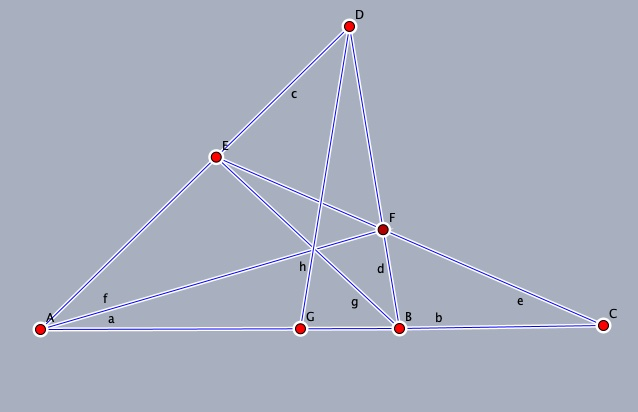
\includegraphics[width=30em]{CompleteQuad3.png} 
   \end{center}
     \protect \caption{A complete quadrilateral, consisting of the four points $A, B, C, D$ and the three lines joining them in pairs}
      \label{figCompleteQuad}
     \end{figure}
\end{center}

\bigskip 
\fix{Note to Editor: In Figure \ref{figCompleteQuad} please relabel the 7 points $A, B, C, D, E, F, G$ as $A, B, E, F, D, C, H$; remove the label $G$; label the point where the lines $AC$ and $BD$ cross (on the new labels) as $G$; delete the lower case letters that label the edges.}




The  \emph{Brouillon Project} is fiercely unreadable.\footnote{Happily, it has been the subject of sequence of detailed analyses in recent papers by Marie  Anglade and Jean-Yves Briend; see (Anglade and Briend 2022) and the references to their earlier papers cited there.} It was also lost for a long time and known only through commentaries by later authors until Michel Chasles found a handwritten copy made by Philippe de la Hire in 1845.\footnote{The only known copy of the original \emph{Brouillon project} turned up in 1950.} In particular, de la Hire, a generation after Desargues, wrote some much more readable, and longer, works in Desargues's spirit, illuminating the role of cross-ratio in the theory of tangents that came close to a theory of duality. Desargues's famous theorem on two triangles in perspective was published separately in (Bosse 1648).

The best attention Desargues's little book got was from his younger contemporary Blaise Pascal, who evidently produced a virtually complete theory of conics around what he called the ``mystical hexagram''. Unhappily, much of it is lost, and known to us only from some notes on it made by Leibniz, but the idea is that while there is always a conic through five points something happens if you want a conic through six points: we call it Pascal's theorem. Then, if you let the sixth point collapse onto one of the other five you get a tangent to the conic through those five points. One way or another all the key properties of conics are wrapped up in this idea, or so Pascal seems to have shown, and much of the early 19th century work in France can be seen as attempts to recover such a theory. It includes such topics as duality, in the form of the pole and polar relationship with respect to a conic (see Figure \ref{figpolepolar}).\footnote{For a thorough analysis of Pascal's work and its context, see (Del Centina 2020).} 


\fix{Note to Editor: In Figure \ref{figpolepolar} please delete the points $A, C, E$; relabel the points $B, D$ as $A, B$; make sure the lines through $A$ and $B$ that are claimed to be tangents really are, and label their point of intersection $P$.}
\bigskip
\begin{center}
    \begin{figure}
   \begin{center}  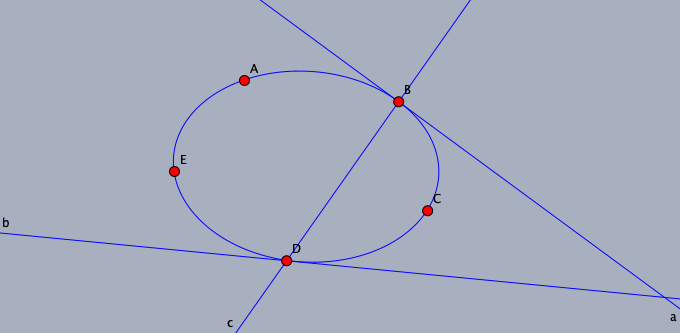
\includegraphics[width=30em]{poleandpolar.png} 
   \end{center}
     \protect \caption{The tangents from a point $P$ outside the conic touch it at $A$ and $B$; the line $AB$ is the \emph{polar} of $P$ and $P$ is the \emph{pole} of the line $AB$. The construction can be extended to points inside the conic.}
      \label{figpolepolar}
     \end{figure}
\end{center}

\bigskip 


Thereafter, truly projective geometry languished for much of the 18th century, despite some insightful contributions by Newton that we shall mention below (see p. ~\pageref{Newtonconics}) and a few others. Its revival is conventionally dated from the early work of Gaspard Monge, who as a young man seeking a job in the French army was  interested in how to depict three dimensions on two. He devised a method of plan and elevation (projections onto a horizontal and a vertical plane) that he could couple to some simple algebra in a way that was easy to use; as a result he was offered a job at the military Academy in M\'ezi\`eres and his discovery made a military secret. During the French Revolution, Monge was influential in setting up the \'Ecole Polytechnique, where he was an inspiring teacher of geometry, and this did much to revive the subject. 

Among those so inspired there was Jean Victor Poncelet, who promoted a much more general theory of transformations with a view to unifying the theory of conics that he began to develop while a prisoner-of-war in Saratov during Napoleon's disastrous invasion of Russia. His \emph{Trait\'e des Propri\'et\'es Projectives des Figures} (1822) is a visionary textbook that relies on some rather mysterious arguments about ideal points of intersection (Cauchy, who reviewed the book, urged that they be regarded as points with complex coordinates; Poncelet never agreed). As a result, some of the transformations it invokes necessarily require complex coordinates. The most famous result in the book is Poncelet's closure theorem, which has continued to attract attention to this day, but it is also notable for many other theorems involving pairs of conics.


In the 1820s, Poncelet had a dispute with Joseph Diaz Gergonne, the editor of the only journal at the time entirely devoted to mathematics, about what duality in the plane actually is.\footnote{Gergonne's journal was called the \emph{Annales de Math\'ematiques Pures at Appliqu\'ees}. It ran from 1810 to 1832, and  it was succeeded in by Liouville's \emph{Journal de Math\'ematiques Pures at Appliqu\'ees} in 1836. Crelle's \emph{Journal f\"ur die reine und angewandte Mathematik} was founded in 1826.}
Poncelet always saw it as pole and polar with respect to a conic, Gergonne saw it as a new and fundamental feature of projective geometry.\footnote{See (Gergonne 1826).} This led into confusion when applying it to curves of degree three or more, a matter that began to be sorted out only with Pl\"ucker's work, as we shall see below.


Another mathematician who was inspired by Monge was the Frenchman Michel Chasles, who used the projective invariance of the cross-ratio of four points to eliminate much of the weirdness of Poncelet's ideas. Independently, Jakob Steiner did very similar work in Germany. He can be credited with the first truly projective definition of a conic section. Even so, there remained an irritating feature of cross-ratio: it was given as a function of four lengths, but length is a property of Euclidean geometry, not projective geometry.  If projective geometry is to be regarded as more fundamental than Euclidean geometry, because it rests on fewer assumptions or axioms, then the intrusion of Euclidean length in the definition of cross-ratio is at the very least unfortunate. Nor can one easily speak of there being a concept of projective space in the 1820s; rather, much of geometry at this time was about figures in the plane subject to a variety of projective transformations. The first truly foundational work on real and complex projective geometry that avoided deriving it from Euclidean geometry was the achievement of von Staudt in his \emph{Geometrie der Lage} (1847), in a long and difficult work that influenced Felix Klein when he succeeded von Staudt as a Professor at Erlangen twenty-five years later. 

All in all, a surprising amount of work was done on the theory of conic sections  at the start of the 19th century, and before it is dismissed as arcane it should be stressed that the subject was a proving ground for the development of projective geometry. Two approaches stand out: the search for entirely  general methods that would treat all non-degenerate conics on a par; and the emergence of the property of duality. Matters are complicated by the existence of two separate traditions, usually called the synthetic and the analytic, supposedly divided into classical geometric methods and more algebraic ones that introduce coordinates. 
Recent historical work suggests that it was all a bit murky, and algebraic methods were also often used in synthetic geometry.\footnote{See (Lorenat 2016).} Several things promoted the use of synthetic methods. They can be elegant when algebraic methods are blunt; they correspond to the visual form of the conics; they provide a language for describing what is apparent or to be found in a problem. Against them is the obstinate fact that algebra is more general: it does not care if some quantities become negative, but what is a negative length? Once ways round that were found (by Poncelet and then Chasles) the way was open to a truly systematic synthetic theory of conics.   

How then did this change, and purely synthetic projective geometry begin to wane? Very few of the original protagonists disdained algebra outright, and as the (projective) theory of conics reached completion in the 1820s and established its fundamental character, being more general than metrical Euclidean geometry, it also had its baroque aspects. But worse, it did not generalise at all readily  to the study of curves of higher degree. For that, as even Newton had recognised, a hefty dose of algebra was required.







\section{Curves of higher degree from the 17th to the early 19th century} A common way to think of curves in antiquity was pointwise: some length depends in a given way on some other length. Accordingly, at least in principle, if you know the independent length
(the ordinate, or $x$ coordinate) you know the dependent length (the abscissa, or $y$ coordinate).  

By Descartes' time there was already some sophisticated algebra expressed in a formalism that hadn't quite shaken off   the Greek insistence on seeing everything as geometrical magnitudes: lengths, areas, volumes, and, well, what exactly? The French mathematician Fran\c{c}ois Vi\`ete in his \emph{Isagoge} boldly spoke of magnitudes having the dimensions of side, square, cube, square-square, square-cube and so on.\footnote{See his collected works, (Vi\'ete 1646).} It was possible to write polynomial equations in this language, as Vi\`ete did in the early 1600s. First Fermat in 1636, and then much more boldly Descartes in 1637, realised that you could extend the language to two variables and so describe curves in the plane.



\bigskip
\begin{center}
    \begin{figure}
   \begin{center}  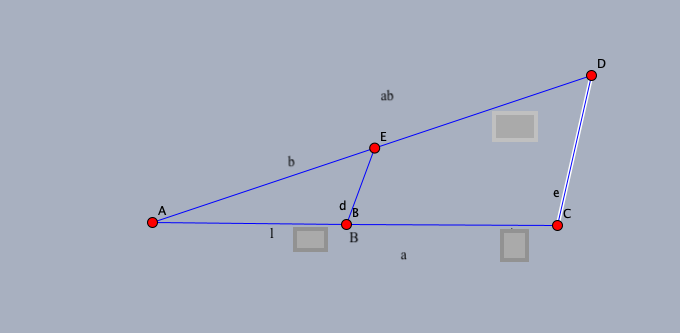
\includegraphics[width=30em]{Multiplication.png} 
   \end{center}
     \protect \caption{If $AB$ is of length 1, $AC$ of length $a$, $AE$ of length $b$, and $BE$ and $CE$ are parallel then AD is of length $ab.$}
      \label{figmultiplication}
     \end{figure}
\end{center}

\bigskip 

\fix{Note to Editor: In Figure \ref{figmultiplication} please move the lower case letters in that denote lengths to better positions, and eliminate the shaded rectangles.}

Descartes's first achievement in his \emph{La G\'eom\'etrie} (1637) was to eliminate the dimensional aspect. A simple use of similar triangles allowed him to show that the product of two lengths could be seen as another length (not an area) so all geometrical quantities could be regarded as one-dimensional and the idea of dimension quietly dropped (see Figure \ref{figmultiplication}). He also replaced Vi\`ete's cumbersome algebra, which was written in capital letters with verbal abbreviations for the algebraic operations, with something much more like   what we use today.  He wrote $x$ and $y$ for the key variables (not $A$ and $E$ in the manner of Vi\`ete). Descartes was clear that he was using coordinates, although his $x$ and $y$ coordinates could have oblique axes.


Then came the real work. Almost all mathematical problems in his day were expressed in the language of geometry, except for some problems we would call diophantine and were implicitly about integers and rational numbers. Accordingly, the answer had to be expressed geometrically. Descartes's idea was to give letters to all the lengths involved in a problem, use the statement of the problem to express relationships between the letters, and reduce the equations to a single equation. Then solve the equation and express the answer again in geometrical terms.  

 In this way he solved the famous Pappus problem (see Figure \ref{figPappusproblem}): given four lines and four angles (nothing is lost if we take these angles to be right angles), find the locus of points $P$ such that the product of the distances of $P$ from the first two lines is proportional to the product of the distances of $P$ from the last two lines. As he showed, and Pappus had known, the answer is a conic section, but  Descartes went further and claimed that in this way he could solve the Pappus problem for any number of lines. 
 
 \bigskip
\begin{center}
    \begin{figure}
   \begin{center}  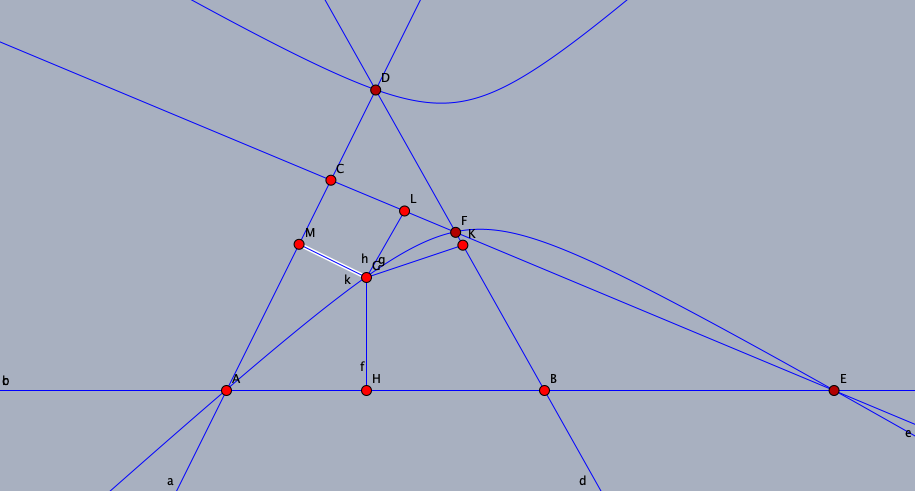
\includegraphics[width=30em]{Pappusproblem.png} 
   \end{center}
     \protect \caption{The Pappus problem: the product of the distances of $P$ from the lines $AB$ and $BC$ is proportional to the product of the distances of $P$ from the lines $CD$ and $DA$}
      \label{figPappusproblem}
     \end{figure}
\end{center}

\bigskip 

\fix{Note to Editor: in Figure \ref{figPappusproblem} please relabel $F$ as $C$, $C$  as $D$, and $G$ as $P$; remove the lower case letters; label the point in the middle $P$, and make sure that the four lines out of $P$ meet the four lines at right angles.}

This was to infuriate Newton, who showed that Greek methods were indeed adequate to the original Pappus problem. The background here is that Newton was also engaged in demolishing Descartes's theory of planetary motion in favour of his own, which led him into the theory of conic sections and to pose and solve the problem of finding the conic (or conics) through $n$ points and tangent to $5-n$ lines, which he did in Book I, Section 5 of his \emph{Principia Mathematica}.~\label{Newtonconics}

It can be argued that the theory of specifically algebraic curves has its origin in Descartes's method for finding normals to a curve at a point, which  involved considering all the circles through the given point and imposing the condition that the equation for the circle be such that it passes twice through the given point; this circle has its centre on the normal to the curve. On the basis of three examples, he claimed that the method always worked  if the curve had an algebraic equation, and he described a system of linkages (sliding rulers) that he said could be adapted to draw any such curve. Curves like the cycloid that were patently not algebraic he sought to exclude from geometry --- this exclusion was something else that annoyed Newton.

In the 1660s and 1670s, but only published  the 1690s and again in 1704 as an Appendix to his \emph{Opticks} Newton worked on a classification of cubic curves. He claimed that there were 72 distinct types which could be derived by simplifying the general equation using what we would call affine or linear transformations, although at one point he used a simple birational transformation. For some reason, in writing up his work for publication he omitted four of the possible cubics, and they were speedily found by various other mathematicians.  Newton also made the striking remark that this collapses to five types if projective transformations are allowed.\footnote{``The five divergent parabolas, by their shadows, generate all other curves of the second genus [i.e. cubic curves].'' See (Newton  1704) and Talbot (1860, p. 25).}





A plane cubic curve is defined by an equation involving ten coefficients, or more precisely by the nine ratios between the coefficients, which suggests that it should be determined by nine points in the plane because their coordinates provide nine equations that should determine these nine ratios.  Moreover, it seemed to mathematicians in the early 18th century that any set of nine points and therefore any set of nine equations in the nine unknowns should have a unique solution --- there was no theory of linear equations at the time ---  and as a result even the best mathematicians got into difficulties. For example, the Scottish mathematician Colin MacLaurin  knew in 1720 that there were problems with the idea that nine points in the plane should determine a cubic: any two cubics will meet in nine points, and so these nine points do not determine a unique cubic, and indeed there will be infinitely many cubics through these nine points.\footnote{MacLaurin also knew that a general cubic curve has nine flexes, and the line joining any two passes through a third.}  MacLaurin did not, however, know how to solve this puzzle. His observation was conveyed to Euler by his friend the Swiss mathematician Gabriel Cramer  in 1744. This apparent contradiction with the claim that nine points in the plane always determine a unique cubic became known as Cramer's paradox.  Part of the confusion at the time was a lack of insight into systems of linear equations, and part was the lack of understanding about what are the implications of configurations that do not determine a unique curve. 

More interestingly, when Cramer addressed the problem in his book (1750, Chapter 3) he suggested that if the $\ha n(n+3)$ points needed to determine a curve of degree $n$ contain $tn$ points common to a curve of degree $t < n$ then the curve through the  $\ha (n+1)(n+2)$ points breaks up into two or more curves, one of which passes through the $tn$ points. We note that Cramer considered only irreducible curves: a circle and a line, for example, would be considered as two curves, not one.\footnote{Curves were taken to be irreducible even in Salmon's book \emph{Higher Plane Curves} (1852).} 


The (incorrect) claim about cubic curves, and more generally the analogous claim for curves of degree $n$, that they are determined by $\ha n(n+3)$ general points, was repeated  by  Euler  in the second volume of his \emph{Introductio} (1748, \S\,81). He then wrote a paper (Euler 1750) in which he first spelled out the problem. It is a general proposition, he said, that $k$ linear equations in $k$ unknowns have a unique solution. Accordingly, 9 points in the plane will determine a unique cubic curve. But nine points common to two cubics plainly do not determine a unique cubic curve. To resolve this apparent contradiction, as he called it, he began with  three equations in three unknowns and showed by example that there will not be a unique solution if one of these equations is contained in (that is, is a consequence of) the others. He drew the same conclusion about four linear equation in four unknowns, and stated more generally that there will not be a unique solution to a system of $n$ equations in $n$ unknowns if one or more are contained in all the others. 

He then turned to the geometrical implications. In the case of conics, he showed that the containment condition corresponds to the case when four, or all five, of five given points lie on a line.  For cubics, he remarked that one easily understands that not just one, but two or more of the nine equations specified by nine points may be contained in the others, and to obtain a unique cubic it will be necessary to specify that the curve passes through one or more additional points.  However, he said, it was very difficult to see what the consequences were when this is the case, because there were so many points and coefficients that things become too complicated, although it was possible to draw conclusions in simple cases. For example, if the nine equations arise in part from four points lying on a line then the remaining five equations must determine a conic, which might itself consist of two lines. Euler concluded his paper with a few remarks about curves of higher degree.


The idea that algebraic curves of degrees $k$ and $m$ in the plane should meet in $km$ points was something of a folklore result in the early 18th century, but it travelled without a proof for many years. Euler discussed it in the second volume of his  \emph{Introductio} (1748, Ch. 19) and noted that even in simple cases  for the counting to work one would have to take care of multiple points (such as tangents),  points `at infinity' (consider a parabola and a line parallel to its axis), and allow the  coordinates of intersection points to be complex (consider the intersection of two circles). The first person to find a persuasive way of tackling the problem was \'Etienne B\'ezout, who lived from 1739 to 1783, and made his living teaching mathematics at the French military and naval academies. He published the theorem that bears his name in a book of 1779; it is based on his theory of the resultant of two polynomial equations that he developed in a paper of 1764. His proof of the theorem is gappy and intuitive by any standards, but so much better than what had been done before that his immediate successors were willing to give him real credit for doing as much as he did. His results inspired later work by Cauchy and Sylvester.

To state  B\'ezout's theorem in general requires a notion of the multiplicity of an intersection of two plane curves without common components. Such a notion was developed by Max Noether, and refined by Macaulay. A modern proof would invoke Noether's Fundamental Theorem --- see p. \pageref{Noether'sFT} --- and a computation of the Hilbert polynomial. This is a story that  has been pursued, with successive new generalisations, right up to the present day. 


As this work suggests, throughout the 18th century mathematicians had become more and more comfortable with the idea of complex numbers in algebra, and with the idea of proving that a polynomial of degree $n$ has $n$ roots, possibly with repetitions (the so-called fundamental theorem of algebra).\footnote{For a history of attempts on this theorem, see (Gilain 1991).} Euler's attitude to complex numbers was that there was nothing to explain. Although they cannot be ordered, expressions of the form $a+bi$  behave arithmetically like numbers, so they can reasonably be considered numbers  and ``are usually called \emph{imaginary quantities}, because they exist merely in the imagination.''\footnote{See Euler, \emph{Algebra} \S\, 143, p. 43. Euler here rejected the idea that ultimately mathematical quantities must be exhibited in nature: three sheep, a length of $\sqrt{2}$, and so on.} Cauchy's view later was more explicit and very close to regarding  the field of complex numbers as $\RR [x]/(x^2 + 1)$. This works for finding a proof of the fundamental theorem of algebra, which he gave a proof of in his (1817a, b), but was not productive in contexts involving contour integration. 

Credit for the first rigorous proof of the fundamental theorem is often given to Gauss for his paper (1799), although he did base his argument on the claim that an algebraic curve that enters a bounded region of the plane also leaves it,  which is surely no easier to prove.  Gauss went on to give three more proofs of the theorem, and soon any doubts about the algebraic nature of complex numbers were resolved.\footnote{William Rowan Hamilton published his rigorous theory of ordered pairs of real numbers in his (1837).} Abel and Jacobi, in their work  on elliptic functions, took a formal, non-geometrical attitude to complex numbers.  Both men were algebraists at heart -- formidable algebraists -- and the exact nature the plane of complex numbers did not really interest them. 

All things considered, however, progress in the study of cubic, quartic, and higher degree curves in the 18th century was piecemeal and slight, and the sheer enormity of the equations involved seems to have baffled even Euler. New methods for handling such curves would have to be found, such as came in with Julius Pl\"ucker in the 1820s. His key idea was to study families of curves, using the symbolic notation devised by Gergonne.\footnote{See  (Gergonne 1826--1827), (Pl\"ucker 1835) and (Pl\"ucker 1839).} If $S_1$ and $S_2$ stand for the equations of two curves of the same degree, then $S_1 + \lambda S_2$ is the equation of another curve of that kind. This may be the first occurrence of the idea of a linear series, with which this book is much concerned. Using this idea allowed Pl\"ucker to pull out geometrical properties of cubic and quartic plane curves while avoiding the algebraic complexities that had defeated Euler.  

Pl\"ucker also resolved the paradox about dual curves in the theory of plane curves in his (1834) that had stumped Gergonne and Poncelet. The paradox arises because the dual of a smooth curve of degree $d$ has degree $d(d-1)$
so the dual of the dual ``ought'' to have degree $d(d-1)(d(d-1)-1)$. However, the dual of the dual is the original curve.  
Pl\"ucker's response, which would strike us today as at best heuristic, was that any line through a double point, say, is counted in this way as a tangent, and this throws the count of genuine tangents off. More precisely, he  showed that each node on a curve reduces the degree of the dual curve by 2, and each cusp reduces it by 3. Consequently, he claimed that  a curve of degree $d$ with $\delta$ double points and $\kappa$ cusps has a dual curve  of degree $d(d-1) -  2\delta - 3\kappa.$ 




Pl\"ucker also showed in his (1839, 207--227) that the nodes of $C^{*}$  corresponded to the bitangents of $C$, while the cusps of $C^{*}$ corresponded to the flexes of $C$, and vice versa. To see how he resolved the duality paradox, consider  the case of a non-singular cubic curve. It has no nodes, cusps, or bitangents, and as yet an indeterminate number, $j$ of flexes. Its dual has degree 6 and $j$ cusps. The dual of the dual curve therefore has degree $6.5 - 3j$, which will equal 3 if $j = 9.$ As we saw, the result that a non-degenerate cubic curve has nine flexes had been known since MacLaurin. For curves of higher degree, it is necessary to consider a curve of degree $n$ that has $\delta$ double points, $\kappa$ cusps, $\tau$ bitangents, and $\iota$ inflections. Suppose that its dual has degree $n'$. Pl\"ucker argued that
\[n' = n(n-1) - 2\delta - 3 \kappa,\]
\[{\rm and}\; \iota = 3n(n-2) - 6\delta - 8\kappa,\]
with another formula for $\tau$, along with the corresponding formula for the dual curve and its inflection points and bitangents.

The number $\iota$ is most easily found using an argument due to Hesse, who showed  in his (1844)  that the set of flexes $\Gamma\subset G$ on a curve $G$ of degree $d$ with equation $F(x, y, z) = 0$ could be characterized as the intersection of $G$  with the curve $D$ defined by the vanishing of the \emph{Hessian determinant}:
$$
H = \det \begin{pmatrix}
 \partial^{2}F/\partial x^{2} &\partial^{2}F/\partial x\partial y &\partial^{2}F/\partial x\partial z \\
\partial^{2}F/\partial x\partial y  &\partial^{2}F/\partial y^{2} &\partial^{2}F/\partial y\partial z \\
\partial^{2}F/\partial x\partial z &\partial^{2}F/\partial y\partial z &\partial^{2}F/\partial z^{2} 
\end{pmatrix}.
$$
Since the entries of this matrix have degree $n-2$, the degree of $H$ is $3(n-2).$ For general $F$ the curves $G$ and $D$ meet transversely, so B\'ezout's Theorem shows that a general curve of degree $m$ has exactly $\iota = 3n(n-2)$ flexes.\footnote{This result was first proved in a different way in (Pl\"ucker 1835, 264), as Hesse acknowledged.}

The most famous case Pl\"ucker established in  his book (1839, 247),  concerns   a nonsingular plane curve $C$ of degree $n=4$  (no nodes, cusps, or other singular points) having $\tau$ bitangents and $\iota$ flexes.   Its dual curve has degree 12 and will have $\tau$ double points and $\iota$ cusps, and the dual of the dual will have degree 
$12\cdot 11 - 2\tau - 3h  = 4.$ 
Hesse's theorem shows that $h = 24$ (Pl\"ucker  had an ad hoc argument to the same effect)  and so $\tau = 28$,  and we  see that $C$ has exactly 28 bitangents. Pl\"ucker showed that they can all be real (see Figure \ref{fig28bitangents}).

In 1849, Pl\"ucker gave up mathematics for physics, particularly the study of cathode rays; he was awarded the Royal Society of London's Copley medal (its highest honour) for this work in 1866. It is sometimes said that he gave up geometry because he tired of the criticisms of Steiner, who had a secure position in Berlin and influenced the decisions of the \emph{Journal f\"ur Mathematik}, and only returned to geometry after Steiner died in 1863. Now he took up  the field of line geometry, which he transformed into a new branch of the subject. 

\bigskip

\begin{center}
    \begin{figure}
   \begin{center}  \includegraphics[width=15em]{28bitangents} 
   \end{center}
     \protect \caption{\, Pl\"ucker's quartic curve has 28 bitangents, from (Pl\"ucker 1839)}
      \label{fig28bitangents}
     \end{figure}
\end{center}
\bigskip

Pl\"ucker's formulae work well for curves of degrees 3 and 4,  but not so well thereafter because other types of singularity can appear.   He listed all the solutions he could find to the equations that bear his name up to curves of degree 10, but he did not discuss the kinds of singularities a curve may have that are not of the type he had considered.\footnote{See (Pl\"ucker 1839, 214).}  Progress was only made with a paper by Cayley (1866), who drew on Puiseux's paper (1850) that analysed  how curves are ramified at a singular point,  showed how the branches are permuted in cycles, and how this is captured by the local power series expansions, which begin with fractional indices.\footnote{Cayley's paper was corrected by Otto Stolz in his (1875), who found that the conclusions were correct but the proof ``as he [Cayley] himself remarks'', was not quite complete.}

Puiseux was one of a number of mathematicians in the circle around Cauchy. Cauchy had spent the 1830s and early 1840s following the Bourbon Court around Europe from a strange belief that the oath of allegiance he had sworn to the crown on becoming a professor compelled him to do so. As a result, by 1850 few people knew the work he had done in those years, and even he seems to have forgotten what he had done in complex variable theory back in the 1820s, which included a version of what we call the Cauchy integral theorem restricted to rectangular contours. Only on his return to Paris did he begin to think much more geometrically; previously his attitude to a many-valued `function' was to cut the plane and study just a branch of it on what remains. His understanding of branch points was quite limited, and this left space for Puiseux to study integrals on arbitrary contours   and what happens to integrals taken around branch points. 

\section{The birth of projective space}
When did projective space come in, regarded as something more rigorous than Euclidean space with a ``line at infinity''?\footnote{For an interesting  set of essays analysing what projective space might be and how it came about, including an extensive analysis by J.-P. Friedelmeyer of the work of Poncelet, see (L. Biosemat-Martagon 2010), and the discussion in del Centina (to appear).}
 This might simply be a suitable set of coordinates. Pl\"ucker used coordinates for the plane with a line at infinity in his (1830) with a view to enabling homogeneous equations to correspond to curves; in this system the coordinates $(p, q, r)$ denote the signed distances of a point from the three sides of a triangle of reference. However, in his study of curves (1835) he would first discuss them in  the plane, and then as they went off to infinity; he didn't say that the line at infinity could be mapped by a projective transformation into the finite part of the plane.  The way forward was indicated by M\"obius, who introduced barycentric coordinates in his (1827). Pick three points forming a triangle, say $ABC$, and attach weights, positive, zero, or negative (not all zero) to these points. The barycentre or centre of gravity of these three weighted points is a point $P$ which can be said to have those three weights (or, better, their ratios) as its barycentric coordinates. If you put the points $A, B, C$ at, say,  $(0, 0), (1, 0), (0, 1)$ you get an easy way to relate points in what could be called the Cartesian and barycentric coordinate planes. The big plus is that the line at infinity, which is invisible in Cartesian coordinates, is a perfectly sensible line in barycentric coordinates. In this system, a line has an equation of the form $ax+by+cz=0,$ and by treating $a, b, c$ as the coordinates of the line M\"obius obtained a simple theory of conics and duality in the plane. (He also showed that there are dualities in $P^3$ that are not pole-polar dualities.)

If you drop the talk about weights, and keep the idea that barycentric coordinates are best thought of as ratios of three numbers, you have projective coordinates; this was one of the contributions of Otto Hesse in the 1840s.\footnote{See, for example, his (1844).}
Mathematicians were still reluctant, however, to decide if this space was $\PP_\RR^2$ or, less likely, $\PP_\CC^2$. 
 


Mathematicians found it  hard to accept complex coordinates,  even though Pl\"ucker used the term `imaginary'  (as in `imaginary' points, `imaginary' straight lines, `imaginary' tangents) over two hundred times in his   (1828--1831).\footnote{Del Centina, forthcoming.} He employed the term confidently in his (1839) when, for example, he discussed how many of the 28 bitangents to a quartic curve can be real. In fact, the whole question of a complex space was obscure for a long time. As late as 1878 Cayley could write about complex curves as sets of points in $\CC \times \CC$ and remark ``I was under the impression that the theory was a known one; but I have not found it set out anywhere in detail.''\footnote{See (Cayley 1878, 32).} For quite some time attention was fixed on real curves in the real plane, which could conveniently sprout points with complex coordinates when they intersected other curves. This unstable situation could not last, but how it was to be swept away was not clear to mathematicians initially. 


\section{Riemann's theory of algebraic curves and its reception}
It was, however, entirely clear to Riemann. The crucial issue in defining complex-valued functions of a complex variable, where a complex variable can be taken as an expression of the form $x+ iy$, is defining what it is for such a function to be something more particular than a mapping from $\RR^2$ to $\RR^2$, and this comes down to defining what it is for such a function to be differentiable as a function of a complex variable. As is well-known, Riemann solved this problem in the opening pages of his inaugural dissertation  (1851) by identifying -- much more clearly than Cauchy -- the role of what we call the Cauchy--Riemann equations. He proceeded to give a thoroughly geometric theory of complex functions, which he extended in his great paper on Abelian functions (1857). There he developed a strikingly topological account, which classified orientable, boundaryless surfaces by the number, $2p+1$, of cuts needs to disconnect them. He called this number the order of connectivity of the surface, when $p=0$ he called the surface simply connected. The theory is too complicated to be described fully here, but briefly, he showed that  the dimension of the space of ``everywhere finite'' differential forms on such a surface is $p$, and the integral of each such 
differential gives rise to a many-valued function, which can be expressed in the form $f(z, w) = 0$, where $z$ and $w$ are complex variables. He also deduced the Riemann inequality in this form (1857, \S\, 5):  the number of arbitrary constants in a function $w$ that has $m$ first-order poles on a surface of order of connectivity $2p+1$ is $m- p + 1$ when $m \geq p + 1$. He gave a more detailed account that involves special cases that were interpreted by his student Roch to give us the Riemann--Roch theorem. 

Riemann's health started to decline in the early 1860s, and he  died in Italy in July 1866. By then, Rudolf Clebsch had decided to develop Riemann's ideas and to try to persuade people around him to take up the cause. In his (1864) he  applied the theory of Abelian functions to the study of plane algebraic curves. Here he used coordinates that belonged  either to $\CC^2$ or $\PP_\CC^2$ and  passed easily between them as required, so it would seem that he and the people he influenced had become comfortable with complex projective space in all but name.

                                                                                                                                                                                                                                                                                                                                                                                                                                                                                                                                                                                                                                                                                                                                                                                                                                                                                                                                                                                                                                                                                                           
In his papers (1865a, 43) and (1865b, 98) Clebsch sorted curves into different genera according to the value of the number $p$ associated to them, but he did not speak of the genus of a curve.\footnote{See (L\^e 2020), who suggests that Felix Klein was the first to do so.} If we allow ourselves to do so, we may say that Clebsch defined the genus of a plane algebraic curve with $\delta$ double points as\footnote{See (Clebsch 1864, 192).} 
 \[p = \ha (n-1)(n-2) - \delta.\]
In his (1865b) and his book with Paul Gordan (1866) he extended this to encompass curves with 
$\kappa$ cusps, so $p= \ha (n-1)(n-2) - \delta - \kappa.$ This tells us incidentally that no singular points more complicated than those considered by Pl\"ucker in the late 1830s had been looked at. Clebsch's formula relied on being able to count the number of constants in an integral of an everywhere finite differential correctly, a result that requires the  completeness of the adjoint series. Clebsch and Gordan, in their book (1866, Chapter 3) offered a proof that the genus of a plane algebraic curve is invariant under a birational transformation, but it was valid only for the case of a curve with simple cusps and double points. 


Clebsch became   Riemann's successor in G\"ottingen in 1868, but  he died of diphtheria in 1872 at the age of 39. His plans for the study of algebraic geometry now devolved upon Alexander Brill and Max Noether, with whose theory, modernised and made rigorous,  this book is in part concerned.\footnote{A modern account of  much of the material described above can be found in (Brieskorn and Kn\"orrer 1986). (Coolidge 1940) remains a historically informative if not entirely rigorous account of many of these developments, more additional mathematical details are in (Coolidge 1931).}

Alexander Wilhelm Brill was born in Darmstadt in 1842.\footnote{See (Severi 1922),  and Brill's obituary (Finsterwalder 1936).} His  uncle was the mathematician Christian Wiener, an expert in descriptive geometry. He entered the University of Giessen intending to study architecture but his mathematical ability brought him to the attention of Clebsch, who was then at Giessen and who encouraged him to go  to Berlin, where  Ernst Kummer,  Leopold Kronecker, and Karl Weierstrass taught. This broadened Brill's horizons considerably, but he returned to Giessen in 1867 to take his Habilitation  under Clebsch.

In Giessen, Brill met Max Noether. Noether had been born in Mannheim in 1844, but polio at the age of 14 left him paralysed in one leg and delayed his education. He had to be privately schooled, which gave him  broad literary and cultural interests. At university he  initially intended to study astronomy, but then he switched to mathematics, first at Heidelberg and then at Giessen and G\"ottingen in 1868 and 1869. He habilitated in Heidelberg in 1870 with a thesis on surfaces possessing a family of rational curves. In 1875 he became a Professor at Erlangen, where he remained until his death in 1921.\footnote{See his obituary (Brill 1923).} 


Noether  worked not only on plane algebraic curves, including the analysis of their singular points, but the geometry of algebraic surfaces,  algebraic curves in space, and Cremona transformations of the plane;  van der Waerden justly remarked that ``Algebraic geometry was created by Max Noether.''\footnote{See (Waerden 1971, 171) who immediately commented that the logical foundations are shaky.} 
He drew largely on the work of Pl\"ucker on algebraic curves and their singular points, and was less interested in the computational side of the theory that Clebsch had emphasised. As a result, his obituarists --- Guido Castelnuovo, Federigo Enriques, and Francesco Severi --- noted that Noether's work was inclined to be qualitatively valuable even though he may not have paid sufficient attention to ``contingent aspects of the formulae''.  However, they added that:\footnote{See (Castelnuovo, Enriques, and Severi 1925, 162)}
\begin{quote}
geometric intuition, which was always his guide, saved him from error, and the work, even if it was not perfect, and perhaps for that reason, was richly suggestive.
\end{quote}



Brill  chafed under the direction of  Richard Baltzer, who was Clebsch's successor at Giessen,  and moved to the new Polytechnic in Darmstadt in 1869, which was academically a step downwards. There, he did his work on the Cayley--Brill correspondence principle, and in 1875  he accepted Klein's offer of becoming a Professor at the Polytechnic in Munich, with responsibility for reforming high school education.  Brill found Klein's inventiveness hard to match, but he enjoyed getting to know some of the other mathematicians there, including Philipp Seidel and the young Alfred Pringsheim. Among his pupils were Walther Dyck, Isaak Bacharach, and Ferdinand Lindemann, who went on to produce the two-volume geometry textbook \emph{Vorlesungen \"uber Geometrie} (known as Clebsch--Lindemann) before achieving fame as the mathematician who proved that $\pi$ is transcendental.


\section{First ideas about the resolution of singular points}
In their work on algebraic curves, Brill and Noether found Riemann's use of the Dirichlet principle at the heart of his theory of complex analytic functions to be unsound, so they studied curves firmly in the complex plane $\CC^2$ or the complex projective plane $\PP_\CC^2.$ They were concerned to treat such curves in full generality, and this led them to confront the issue of arbitrary singularities of plane curves. Their preferred method was to argue that any curve with whatever singularities could be reduced to one of the same genus but having only double points by a sequence of Cremona transformations, and then to deal in detail with these simpler curves. It was clear from the formula for the genus of a plane curve that if the genus of the curve is not a triangular number then the curve will always have singular points, so the process of desingularising cannot always lead to a nonsingular curve.

Luigi Cremona had  outlined a general theory of transformations of the plane in his papers (1863) and (1865). He looked for geometrical transformations of the plane mapping a given figure one-to-one onto its image, and reciprocally; notably  transformations that map straight lines to curves of order $n$, for some $n.$ When $n=2$ (the case of quadratic transformations)  as he showed, almost all straight lines must have images that are conics passing through 3 fixed points.\footnote{Such examples had been studied before, Cremona  cited papers by Steiner, Magnus, and Schiaparelli, but for higher values of $n$, which Cremona analysed in his (1865), everything was new.}



Noether in his (1871a) was the first to appreciate that Cremona transformations could be used to simplify singular points.  He wrote a Cremona transformation of the plane algebraically as 
\[[x, y, z] \mapsto [x', y', z'] = [\phi (x, y, z), \psi (x, y, z),  \chi (x, y, z)], \]
where the functions $\phi, \psi$ and $\chi$ are homogeneous polynomials in $x, y$ and $z$ of the same degree. To simplify a singular point he used
transformations defined as above where $\phi, \psi$, and $\chi$ all vanish at the singular point.  In the affine plane this becomes
\[(x , y) \mapsto (x_1 , y_1) = \left(\frac{\varphi (x, y)}{\chi (x, y)}\;,  \frac{\psi (x, y)}{\chi (x, y)} \right),\]
where $\varphi$, $\psi$, and $\chi$ are polynomial functions that vanish at the singular point.  To see what this does, it is convenient to take the familiar example of 
the simplest  Cremona transformation, other than a projective transformation. It  is given algebraically by  the quadratic transformation 
\begin{equation}~\label{eq:qt1}
[x, y, z] \mapsto \left[\frac{1}{x}, \frac{1}{y}, \frac{1}{z}\right] = [yz, zx, xy]\end{equation}
The union of the lines $x=0,y=0,z=0$ is called the exceptional triangle, and the images of these lines are the points $[1, 0, 0], [0, 1, 0]$ and $[0, 0, 1]$ respectively.
The transformation is many-valued at these points, each of which is ``blown up'' into a line  but it is well-defined away from those three points and it is  one-to-one away from  the lines $x=0$, $y=0$, and $z = 0.$ 


Noether's argument that any plane algebraic curve can be reduced to one with only double points is sketchy at best. His use of Puiseux's work suggests that he appreciated that quadratic transformation might have to be used repeatedly to reduce a complicated singularity to a simpler one, but he did not  fully appreciate what happens to the rest of the curve at the points where it crosses the exceptional lines. In his more rigorous account  (1876),  he gave a better definition of a singular point, and tried to redefine the genus of a plane algebraic curve and prove its  invariance  under birational  transformations.\footnote{Noether also claimed  the remarkable theorem that every such Cremona transformation is a composition of quadratic transformations and projective transformations. See his (1871b), with a small correction in his (1873).} 


\section{The work of Brill and Noether}
Noether began, in his (1873), with the question of when  a plane curve $E$ with equation $H=0$ can be expressed in the form $H = AF+BG,$ where $F=0$ and $G=0$ are the equations of two curves $C$ and $D.$ He rightly pointed out that people hitherto had assumed that it was necessary and sufficient that the curve $E$  passes simply through the intersection points of the curves $C$ and $D$, but in fact this is insufficient when the curves $C$ and $D$ have singular points or intersections with multiple tangents. His own account, which was based on counting the number of independent equations imposed on $H=0$ by the equations $F=0$ and $G=0$, was a significant advance, but it too had flaws and he and other authors, notably Bertini, offered improvements. Eventually, Noether  offered this formulation of his  Fundamental Theorem\label{Noether'sFT}:\footnote{See (Noether 1887, 413).}
\begin{theorem}~\label{NFT1887}
$H(x, y)$ is representable in the form $AF + BG$ if and only if in some neighbourhood of each common point $(x_0, y_0)$ of $F=0$ and $G=0$ there are power series $a(x-x_0)$ and $b(x-x_0)$ in $\CC[y][[x]]$ whose coefficients are polynomials in $y$ of orders  $n-1$ and $m-1$ respectively, such that $H = aF + bG.$ 
\end{theorem}
Only in the monumental joint work with Brill (Brill and Noether 1894, 352) was it shown that in the plane case there is nothing more to be said, the local conditions are indeed sufficient even in the projective case.


Today we would say that Noether's Fundamental Theorem is true for two polynomials $F$ and $G$ because $F,G$ is a regular sequence  and so  the ideal they generate is, in later terminology due to Macaulay (1916), unmixed.\footnote{See (Eisenbud and Gray 2023) and (Eisenbud and Gray 2024) for a historical account of Macaulay's work.}


Brill and Noether recognised that the Riemann-Roch Theorem, was of  central importance to the theory of plane algebraic curves; indeed, they were the first to name it.\footnote{See (Brill and Noether 1874, \S\,5).}  Clebsch had studied what we would call holomorphic differential forms on a curve $C$  of degree $d$ in his (1864, 193)  by supposing that they are given by homogeneous polynomials of degree $d-3$ that vanish at the double points of the curve. 
By B\'ezout's Theorem, such an intersection also has degree $d(d-3) = 2p-2$, as it should. The dimension of the family of divisors cut out on $C$ in this way is the dimension of the projective space of forms of degree $d-3$ in $\CC[x_0,x_1,x_2]$, which is conveniently equal to $(d-1)(d-2)/2$. For this to be correct and account for all the canonical divisors, it has to be shown that every divisor $E$ on the curve $C$ that differs from an intersection $D\cap C$, where $D$ is the curve defined by the equation $G = 0$,  by the divisor of the restriction to $C$ of a rational function $P/Q$ (where $P, Q$ are forms of the same degree), is again of the form $D'\cap C$ for some curve $D'$. This is the content of Noether's Fundamental Theorem. His Fundamental Theorem is essential when it comes  to handling  sets of points cut out on a fixed curve $C$ by families of curves, counting the degree of an intersection of two curves at multiple points,  dividing an arbitrary intersection into two subsets, and delivering a satisfactory version of the Riemann-Roch Theorem. 












 

\section{Bibliography}
\small
\indent Anglade, M. and J.-Y. Briend 2022. Nombrils, bruslans, autrement foyerz; la g\'eom\'etrie en action dans le \emph{Brouillon project} de Girard Desargues, \emph{Archive for History of Exact Sciences}, 76, 173--206.
\newline\indent B\'ezout, E. 1764. Sur le degr\'e des \'equations r\'esultantes de l'\'evanouissment des inconnues, \emph{M\'emoires de l'Acad\'emie Royale des Sciences}, 288--338.
\newline\indent B\'ezout, E. 1779. \emph{Th\'eorie g\'en\'erale des \'equations alg\'ebriques}, Ph.-D. Pierres, Paris, 1779. English translation by Eric Feron, Princeton University Press, 2006.
\newline\indent  Biosemat-Martagon, L. 2010. \emph{El\'ements d'une biographie de l'Espace projectif}, Presses Universitaires de Nancy.
\newline\indent Bombelli, R. 1572 \emph{L'algebra}, Bologna.
\newline\indent Bosse, A.  1648. \emph{Maniere universelle de Mr. Desargues pour pratiquer la perspective, etc}, Paris.
\newline\indent Brieskorn, E. and  H. Kn\"orrer 1986. \emph{Plane Algebraic Curves} Birhh\"auser.
\newline\indent Brill, A. 1923. Max Noether, \emph{Jahrsbericht den Deutschen mathematiker Vereinigung} 32, 211--233.
\newline\indent Brill, A. and M. Noether  1874.  Ueber die algebraischen Functionen und ihre Anwendung in der Geometrie, \emph{Mathematische Annalen} 7, 269--310.
\newline\indent Brill A. and M. Noether 1894  Die Entwicklung der Theorie der algebraischen Functionen in alterer und neuerer Zeit, \emph{Jahrsbericht den Deutschen mathematiker Vereinigung} 3, 107--566.
\newline\indent Cardano, G. 1545  \emph{Artis Magnae sive de regulis algebraicis liber unus}, Nuremburg. 
\newline\indent Castelnuovo, G., F. Enriques, and F. Severi, 1925 Max Noether, \emph{Mathematische Annalen} 93, 161--181.
\newline\indent Cauchy, A.-L. 1817a. Sur les racines imaginaires des \'equations. \emph{Nouv. Bull. Soc. Philom.} 5--9, in  \emph{Oeuvres Compl\`etes} (2) 2, 210--216.
 \newline\indent Cauchy, A.-L. 1817b. Seconde note sur les racines imaginaires des\'equa\-tions. \emph{Nouv. Bull. Soc. Philom.} 161--164, in \emph{Oeuvres Compl\`etes} (2) 2, 217--222.
\newline\indent Cayley, A. 1866. On the higher singularities of a plane curve, \emph{Quarterly Journal of Pure and Applied Mathematics} 7, 212--223, in \emph{Collected Mathematical Papers} V, no. 374, 520--582.
\newline\indent   Cayley, A. 1878. On the geometrical representation of imaginary variables by a real correspondence of two planes, \emph{Proceedings of the  London Mathematical Society} 9, 31--39 in \emph{The Collected Mathematical Papers of Arthur Cayley} X, no. 689, 316--323.
\newline\indent Chasles, M. 1837.  \emph{Aper\c{c}u historique sur l'origine et le d\'eveloppement des m\'ethodes en g\'eom\'etrie}, Hayez, Bruxelles. 
\newline\indent Clebsch, R.F.A. 1864.  Ueber die Anwendung der Abelschen Functionen in der Geometrie, \emph{Journal f\"ur die reine und angewandte Mathematik}  63, 189--243.
\newline\indent Clebsch, R.F.A. 1865a. Ueber die diejenigen ebenen Curven, deren Coordinaten rationale Functionen eines Parameters sind \emph{Journal f\"ur die reine und angewandte Mathematik} 64, 43--65.
\newline\indent Clebsch, R.F.A. 1865b. Ueber die Singularit\"aten algebraischer Curven, \emph{Journal f\"ur die reine und angewandte Mathematik} 64, 98--100.
\newline\indent Clebsch, A. and P. Gordan 1866. \emph{Theorie der Abelschen Functionen}, Teubner, Leipzig.
\newline\indent Cohen, M.R. and Drabkin, I.E. 1948. \emph{A Source Book in Greek Science}, Harvard University Press.
\newline\indent Coolidge, J.L.  1931 \emph{A Treatise on Algebraic Plane Curves} Oxford U.P. , Dover reprint 2004.
\newline\indent Coolidge, J.L.  1940  \emph{A history of geometrical methods}, Oxford U.P., Dover reprint 2003.
\newline\indent Cramer, G. 1750. \emph{Introduction \`a l'analyse des lignes courbes alg\'ebriques}. Fr\`eres Cramer et Cl. Philibert, Geneva.
\newline\indent Del Centina, A. 2020 Pascal's Mystic Hexagram, and a conjectural restoration of his lost Treatise on Conic Sections. \emph{Archive for History of Exact Sciences} 74.5, 469--521.
\newline\indent Desargues G. 1639. \emph{Brouillon project d'une atteinte aux evenements des rencontres du Cone avec un Plane}, Paris.  J.V. Field  and J.J. Gray (eds. and transl.)\emph{The geometrical work of Girard Desargues}, 1987, Springer, New York.
\newline\indent Descartes, R. 1637 \emph{La G\'eom\'etrie} in \emph{Discours de la M\'ethode, etc.} Leyden, English transl. \emph{The Geometry of Ren\'e Descartes}, D.E. Smith and M.L. Latham, Open Court 1925, Dover reprint 1954.
\newline\indent Eisenbud, D.E. and J.J. Gray, 2023 F.S. Macaulay: From plane curves to Gorenstein rings, \emph{Bulletin (new series) of the American Mathematical Society} 
60.3,  371?406, https://doi.org/10.1090/bull/1787
\newline\indent Eisenbud, D.E. and J.J. Gray, to appear \emph{F. S. Macaulay: from plane geometry to modern commutative algebra}
\newline\indent  Euler, L. 1748. \emph{Introductio in Analysin Infinitorum}, two vols., \emph{Opera Omnia} (1) Vols. 8 and 9, transl. \emph{Introduction to Analysis of the Infinite}, Book I,  Springer, 1988, Book II, Springer, 1990 (E101, E102).
\newline\indent  Euler, L. 1750.  Sur un contradiction apparente dans la doctrine des lignes courbes. \emph{M\'emoires de l'Acad\'emie des Sciences de Berlin} 4, 1750, 219--233, in  \emph{Opera Omnia} (1)   26, 33--45 (E147).
\newline\indent Euler, L. 1770. \emph{Vollst\"andige Einleitung zur Algebra} in \emph{Opera Omnia} (1) 1,  transl. \emph{Elements of Algebra}, Rev. J. Hewlett, London, 1840, repr.  Springer, 1972 (E387).
\newline\indent Finsterwalder, S. 1936 Alexander v. Brill. Ein Lebensbild, \emph{Mathematische Annalen} 112, 653--663.
\newline\indent Gauss, C.F.  1799. Demonstratio nova theorematis omnem functionem algebraicam \ldots resolvi posse, Helmstadt, in \emph{Werke} III, 1--30.
\newline\indent Gergonne, J.D. 1826. Philosophie math\'ematique. Consid\'erations philo\-sophiques sur les \'el\'emens de la science de l'\'etendue, \emph{Annales de Math\'ematiques} 16, 209--231.
\newline\indent Gergonne, J.D. 1826--1827. Recherches sur quelques lois g\'en\'erales qui r\'egissent les lignes et surfaces alg\'ebriques de tous les ordres. \emph{Annales de Math\'ematiques}17, 214--252. 
 \newline\indent  Gilain, Ch. 1991. Sur l'histoire du th\'eor\`eme  fondamental de l'alg\`ebre: th\'eorie des \'equations et calcul int\'egral, \emph{Archive for History of Exact Sciences} 42, 91--136. 
 \newline\indent Hamilton, W.R.  1837. Theory of conjugate functions, or algebraic couples; with a preliminary and elementary essay on algebra as the science of pure time, \emph{Transactions of Royal Irish Academy}  17, 293--422. 
 \newline\indent Heath, Sir T.L. 1921. \emph{A History of Greek mathematics}, 2 vols, Clarendon Press, Oxford, repr. Dover, 1981.
 \newline\indent Hesse, O. 1844. Ueber die Wendepunkte der  Curven dritter Ordnung \emph{Journal f{\"u}r die reine und angewandte Mathematik} 28, 97--107, in \emph{Gesammelte Werke}, 123--136.
\newline\indent  Hesse, L. O. 1855. Ueber die Doppeltangenten der Curven vierter Ordnung. \emph{Journal f{\"u}r die reine und angewandte Mathematik} 49, 243--264, in \emph{Gesammelte Werke}, 319--344.
\newline\indent Hesse, L. O. 1897. \emph{Gesammelte Werke}. Verlag der K.  Akademie, M\"{u}nchen. Repr. Chelsea, New York 1972.
\newline\indent al-Kh\={a}yyam\={i}, `Umar 1950. In H.J.J. Winter and W. Arafat, The Algebra of Omar Khayy\={a}m, \emph{Journal of the Royal Asiatic Society of Bengal}, 16, 27--78.
 \newline\indent Knorr, W.R.  1986. \emph{The Ancient Tradition of Geometric Problems}, Birkh\"auser, Dover reprint, 1993.
 \newline\indent L\^e, F. 2020 ``Are the genre and the Geschlecht one and the same number?'' An inquiry into Alfred Clebsch's Geschlecht, \emph{Historia Mathematica} 53, 71--107.
 \newline\indent Lorenat, J. 2016 Synthetic and analytic geometries in the publications of Jakob Steiner and Julius Pl\"ucker (1827--1829) \emph{Archive for History of Exact Sciences}  70.4, 413--462
 \newline\indent Macaulay, F.S.  1916  \emph{The algebraic theory of modular systems},  Cambridge Tracts in Mathematics, No. 19.
\newline\indent  MacLaurin, C. 1720.  \emph{Geometria Organica, sive Descriptio Linearum Curvarum Universalis}, London.
 \newline\indent Maurolico, F. 1611 \emph{Theoremata de lumine et umbra}. 
 \newline\indent M\"obius, A.F. 1827. \emph{Der Barycentrische Calcul}, Barth, Leipzig.
\newline\indent Newton, Sir I. 1687. \emph{Philosophiae  Naturalis Principia Mathematica} London, 2nd edn. 1713, 3rd edn. 1726. English translation \emph{Isaac Newton's Philosophiae Naturalis Principia Mathematica. The third edition, 1726, with variant readings}, I.B. Cohen and A. Whitman (transls. and eds.), Cambridge University Press, 1972, 1999.
\newline\indent Newton, I. 1704. \emph{Enumeratio linearum tertii ordinis}, appendix in \emph{Opticks}, London. English transl. \emph{Sir Isaac Newton's Enumeration of Lines of the third Order} C.R.M. Talbot, 1860.
\newline\indent Noether, M. 1871a Ueber die algebraischen Functionen einer und zweier Variabeln, \emph{Nachrichten von der K\"oniglichen Gesellschaft der Wissenschaften und der Georg-Augusts Universit\"at zu G\"ottingen} 267--278.
\newline\indent Noether, M. 1871b Ueber Fl\"achen, welche Schaaren rationaler Curven besitzen, \emph{Mathematische  Annalen} 3,   161--227 and 547--580.
\newline\indent Noether, M. 1873 Ueber einen Satz aus der Theorie der algebraischen Functionen, \emph{Mathematische Annalen} 6, 351--359.
\newline\indent Noether, M. 1876  Ueber die singul\"aren Werthsysteme einer algebraischen Function und die singul\"aren Punkte einer algebraischen Curve, \emph{Mathematische  Annalen} 8, 166--182.
\newline\indent Noether, M. 1887 Ueber den Fundamentalsatz der Theorie der
algebraischen Functionen,  \emph{Mathematische Annalen} 30, 410--417. 
\newline\indent Pl\"ucker, J. 1829a, b. Recherches sur les courbes alg\'ebriques de tous les degr\'es, \emph{Annales de Math\'e\-matiques Pures et Appliqu\'ees} 19, 97--106 and 129--137.
\newline\indent Pl\"ucker, J. 1830. \"Uber ein neues Coordinatensystem, \emph{Journal f\"ur die reine und angewandte Mathematik} 5, 1--36.
\newline\indent Pl\"ucker, J. 1828--1831.  \emph{Analytisch-geometrische Entwicklung}, 2 vols. Essen. 
\newline\indent Pl\"ucker, J. 1834. Solution d'une question fondamentale concernant la th\'eorie g\'en\'erale des courbes, \emph{Journal f\"ur die reine und angewandte Mathematik} 12, 105--108.
\newline\indent Pl\"ucker, J. 1835. \emph{System der analytischen Geometrie}, Berlin.
\newline\indent Pl\"ucker, J. 1839. \emph{Theorie der algebraischen Curven}, Bonn.
\newline\indent Poncelet, J.V. 1822. \emph{Trait\'{e} des Propri\'{e}t\'{e}s Projectives des Figures}, Gauthier-Villars, Paris.
\newline\indent Puiseux, V. 1850. Recherches sur les fonctions alg\'ebriques, \emph{Journal de Math\'ematiques Pures et Appliqu\'ees} 15, 365--480.
\newline\indent Riemann, B. 1851.  Grundlagen f\"ur eine allgemeine Theorie der Functionen einer ver\"anderlichen complexen Gr\"osse (Inaugural dissertation), G\"ottingen, in \emph{Mathematische Werke}, 3--45.
 \newline\indent Riemann, B. 1857  Theorie der Abelschen Functionen, \emph{Journal f\"ur die reine und angewandte Mathematik}  54, 115--155, in \emph{Mathematische Werke} 88--144.
 \newline\indent  Riemann, B. 1990. \emph{Bernhard Riemann's Gesammelte Mathematische Werke und Wissenschaft\-liche Nachlass}, R. Dedekind and  H. Weber (eds.)  with Nach\-tr\"age, M. Noether and W. Wirtinger (eds.). 3rd edn. R. Narasimhan (ed.), Springer, 1990.
 \newline\indent Severi, F. 1922  Alexander von Brill zum achtzigsten Geburtstag am 20, September 1922, \emph{Jahrsbericht den Deutschen mathematiker Vereinigung} 31, 89--96.
  \newline\indent Staudt, K.C.G. von, 1847. \emph{Geometrie der Lage}, Nuremberg.
\newline\indent   Steiner, J. 1832. \emph{Systematischer Entwickelung der Abh\"angigkeit geometri\-scher Gestalten von einander}, Fincke.
 \newline\indent Stolz, O.  1875. Ueber die singul\"aren Punkte der algebraischen Functionen und Curven, \emph{Mathematische Annalen} 8, 415--443. 
\newline\indent Thomas, I. 1939. \emph{Selections Illustrating the History of Greek Mathematics}, (2nd edn. 1980), Heinemann.
 \newline\indent Vi\`ete  F. 1646.  \emph{Opera Mathematica \ldots Recognita Opera}, F.  Schooten (ed.), Lugduni Batavorum.
\newline\indent Van der Waerden, B.L. 1961. \emph{Science Awakening}, A. Dresden (transl.), Oxford University Press.
\newline\indent Waerden, B.L. van der, 1971  The Foundations of Algebraic Geometry from Severi to Andr{\'e} Weil, \emph{Archive for History of Exact Sciences} 7,  171--180, in  \emph{Zur algebraische Geometrie},  1--10, Springer, 1983.
 \normalsize
 
 
 
 
 
 







%footer for separate chapter files

\ifx\whole\undefined
%\makeatletter\def\@biblabel#1{#1]}\makeatother
\makeatletter \def\@biblabel#1{\ignorespaces} \makeatother
\bibliographystyle{msribib}
\bibliography{slag}

%%%% EXPLANATIONS:

% f and n
% some authors have all works collected at the end

\begingroup
%\catcode`\^\active
%if ^ is followed by 
% 1:  print f, gobble the following ^ and the next character
% 0:  print n, gobble the following ^
% any other letter: normal subscript
%\makeatletter
%\def^#1{\ifx1#1f\expandafter\@gobbletwo\else
%        \ifx0#1n\expandafter\expandafter\expandafter\@gobble
%        \else\sp{#1}\fi\fi}
%\makeatother
\let\moreadhoc\relax
\def\indexintro{%An author's cited works appear at the end of the
%author's entry; for conventions
%see the List of Citations on page~\pageref{loc}.  
%\smallbreak\noindent
%The letter `f' after a page number indicates a figure, `n' a footnote.
}
\printindex[gen]
\endgroup % end of \catcode
%requires makeindex
\end{document}
\else
\fi


\makeatletter \def\@biblabel#1{\ignorespaces} \makeatother
\bibliographystyle{msribib}
\bibliography{slag}



\end{document}


%% EXPLANATIONS:

% f and n
% some authors have all works collected at the end

\begingroup
%\catcode`\^\active
%if ^ is followed by 
% 1:  print f, gobble the following ^ and the next character
% 0:  print n, gobble the following ^
% any other letter: normal subscript
%\makeatletter
%\def^#1{\ifx1#1f\expandafter\@gobbletwo\else
%        \ifx0#1n\expandafter\expandafter\expandafter\@gobble
%        \else\sp{#1}\fi\fi}
%\makeatother
\let\moreadhoc\relax
\def\indexintro{%An author's cited works appear at the end of the
%author's entry; for conventions
%see the List of Citations on page~\pageref{loc}.  
%\smallbreak\noindent
%The letter `f' after a page number indicates a figure, `n' a footnote.
}
\printindex[gen]
\endgroup % end of \catcode
%requires makeindex


